%% This is file `dvipdfmx.def' for DVIPDFMx by J.-H. Cho and S. Hirata
%% which is written based on `dvipdf.def' in the LaTeX `Graphics Bundle'.
%%
%% This is file `dvipdf.def',
%% generated with the docstrip utility.
%%
%% The original source files were:
%%
%% drivers.dtx  (with options: `dvipdf,color1,psrulesZ')
%% 
%% drivers.dtx Copyright (C) 1994      David Carlisle Sebastian Rahtz
%%             Copyright (C) 1995 1996 1997 1998 1999 David Carlisle
%%
%% This file is part of the Standard LaTeX `Graphics Bundle'.
%% It may be distributed under the terms of the LaTeX Project Public
%% License, as described in lppl.txt in the base LaTeX distribution.
%% Either version 1.0 or, at your option, any later version.
%%
\ProvidesFile{dvipdfmx.def}
        [1999/02/16 v3.0i Driver-dependant file (DPC,SPQR)]
\def\c@lor@arg#1{%
  \dimen@#1\p@
  \ifdim\dimen@<\z@\dimen@\maxdimen\fi
  \ifdim\dimen@>\p@
    \PackageError{color}{Argument `#1' not in range [0,1]}\@ehd
  \fi}
\def\color@gray#1#2{%
  \c@lor@arg{#2}%
  \edef#1{[#2]}%
  }
\def\color@cmyk#1#2{\c@lor@@cmyk#2\@@#1}
\def\c@lor@@cmyk#1,#2,#3,#4\@@#5{%
  \c@lor@arg{#4}%
  \c@lor@arg{#1}%
  \c@lor@arg{#2}%
  \c@lor@arg{#3}%
  \edef#5{[#1 #2 #3 #4]}%
  }
\def\color@rgb#1#2{\c@lor@@rgb#2\@@#1}
\def\c@lor@@rgb#1,#2,#3\@@#4{%
  \c@lor@arg{#1}%
  \c@lor@arg{#2}%
  \c@lor@arg{#3}%
  \edef#4{[#1 #2 #3]}%
  }
\def\color@RGB#1#2{\c@lor@@RGB#2\@@#1}
\def\c@lor@@RGB#1,#2,#3\@@#4{%
 \c@lor@RGB@rgb{#1}\@tempa
 \c@lor@RGB@rgb{#2}\@tempb
 \c@lor@RGB@rgb{#3}\@tempc
 \c@lor@@rgb\@tempa,\@tempb,\@tempc\@@#4%
  }
\def\c@lor@RGB@rgb#1#2{%
  \dimen@#1\p@
  \divide\dimen@\@cclv
  \edef#2{\strip@pt\dimen@}}
\def\color@hsb#1#2{\c@lor@@hsb#2\@@#1}
\def\c@lor@@hsb#1,#2,#3\@@#4{%
  \c@lor@arg{#1}%
  \c@lor@arg{#2}%
  \c@lor@arg{#3}%
  \edef#4{[#1 #2 #3] hsb}%
  }
\def\color@named#1#2{\c@lor@@named#2,,\@@#1}
\def\c@lor@@named#1,#2,#3\@@#4{%
  \@ifundefined{col@#1}%
    {\PackageError{color}{Undefined color `#1'}\@ehd}%
  {\edef#4{ #1}}%
  }
\def\c@lor@to@ps#1 #2\@@{\csname c@lor@ps@#1\endcsname#2 \@@}
\def\c@lor@ps@#1 #2\@@{TeXDict begin #1 end}
\def\c@lor@ps@rgb#1\@@{#1 setrgbcolor}
\def\c@lor@ps@hsb#1\@@{#1 sethsbcolor}
\def\c@lor@ps@cmyk#1\@@{#1 setcmykcolor}
\def\c@lor@ps@gray#1\@@{#1 setgray}
\def\current@color{[0]}
\def\set@color{%
            \special{pdf:bcolor \current@color
                          }\aftergroup\reset@color}
\def\reset@color{\special{%
         pdf:ecolor}}
\def\set@page@color{\special{%
         pdf:bgcolor \current@color}}
\def\define@color@named#1#2{%
  \expandafter\let\csname col@#1\endcsname\@nnil}
\def\Ginclude@eps#1{%
 \message{<#1>}%
  \bgroup
  \def\@tempa{!}%
  \dimen@\Gin@req@width
  \dimen@ii.1bp%
  \divide\dimen@\dimen@ii
  \@tempdima\Gin@req@height
  \divide\@tempdima\dimen@ii
    \special{PSfile="#1"\space
      llx=\Gin@llx\space
      lly=\Gin@lly\space
      urx=\Gin@urx\space
      ury=\Gin@ury\space
      \ifx\Gin@scalex\@tempa\else rwi=\number\dimen@\space\fi
      \ifx\Gin@scaley\@tempa\else rhi=\number\@tempdima\space\fi
      \ifGin@clip clip\fi}%
  \egroup}
\def\Ginclude@bmp#1{%
 \message{<#1>}%
  \bgroup
  \def\@tempa{!}%
    \special{pdf:image\space
      width  \the\Gin@req@width\space
      height \the\Gin@req@height\space
      (#1)}%
  \egroup}
\def\Grot@start{%
\special{pdf:btrans rotate \Grot@angle}}
\def\Grot@end{\special{pdf:etrans}}
\def\Gscale@start{%
\special{pdf:btrans xscale \Gscale@x\space yscale \Gscale@y}}
\def\Gscale@end{\special{pdf:etrans}}
\def\Gin@PS@raw#1{\special{ps: #1}}
\def\Gin@PS@restored#1{\special{" #1}}%"
\def\Gin@PS@literal@header#1{\AtBeginDvi{\special{! #1}}}
\def\Gin@PS@file@header#1{\AtBeginDvi{\special{header=#1}}}
\@namedef{Gin@rule@.jpg}#1{{bmp}{.bb}{#1}}
\@namedef{Gin@rule@.jpeg}#1{{bmp}{.bb}{#1}}
\@namedef{Gin@rule@.png}#1{{bmp}{.bb}{#1}}
\@namedef{Gin@rule@.bmp}#1{{bmp}{.bb}{#1}}
%\def\Gin@extensions{.eps,.ps,.eps.gz,.ps.gz,.eps.Z}
\def\Gin@extensions{.jpg,.jpeg,.png,.bmp,.pdf,.eps,.ps,.eps.gz,.ps.gz,.eps.Z}
%\@namedef{Gin@rule@.pdf}#1{{bmp}{.bb}{#1}}
\@namedef{Gin@rule@.pdf}#1{{eps}{.bb}{#1}}
%
\@namedef{Gin@rule@.ps}#1{{eps}{.ps}{#1}}
\@namedef{Gin@rule@.eps}#1{{eps}{.eps}{#1}}
\@namedef{Gin@rule@.pz}#1{{eps}{.bb}{`gunzip -c #1}}
\@namedef{Gin@rule@.eps.Z}#1{{eps}{.eps.bb}{`gunzip -c #1}}
\@namedef{Gin@rule@.ps.Z}#1{{eps}{.ps.bb}{`gunzip -c #1}}
\@namedef{Gin@rule@.ps.gz}#1{{eps}{.ps.bb}{`gunzip -c #1}}
\@namedef{Gin@rule@.eps.gz}#1{{eps}{.eps.bb}{`gunzip -c #1}}
\@namedef{Gin@rule@*}#1{{eps}{\Gin@ext}{#1}}
\endinput
%%
%% End of file `dvipdfmx.def'.

\documentclass[9pt,a5j,dvipdfmx,papersize]{jsbook}[2006/01/21]%
\usepackage[phiragino]{joumac}[20006/03/02]% + hyper
%\includeonly{10apply}
\setlength \overfullrule {5pt}
\begin{document}%
\author          {渡辺徹}%
\title           {好き好き\LaTeXe 初級編}%
\date            {\today}%
\def\genzai      {2006年4月現在}%
\FileVersion     {1.13}%
\copyrightAuthor {渡辺徹}%
\copyrightYear   {2004, 2005, 2006}%
\eauthor         {Thor Watanabe}%
\etitle          {Love Love LaTeX 2e}%
\esubject        {for beginners}%
\ekeywords       {TeX, LaTeX, LaTeX2e, pTeX, pLaTeX, pLaTeX2e, FUNNIST, thesis}%
\contact         {Th\'or Watanabe\\% 連絡先
                  Graduate School of System Information Science\\%
                  Future University-Hakodate\\%
                  thor at tex dot dante dot jp\\%
                  \url{http://tex.dante.jp/typo/}}%
\ProvidesFile{settings.tex}
\makeatletter
\ifHyper
% 意図
\def\@setref#1#2#3{% csname, extract group, refname
  \ifx#1\relax
    \protect\G@refundefinedtrue
    \nfss@text{\reset@font\bfseries ??}%
    \@latex@warning{%
      Reference `#3' on page \thepage \space undefined%
    }%
  \else
    \hyper@@link
      {\expandafter\@fifthoffive#1}%
      {\expandafter\@fourthoffive#1\@empty\@empty}%
      {\expandafter#2#1\@empty\@empty \spacefactor \@m}%
  \fi
}
\def\auto@setref#1#2#3{% csname, extract group, refname
  \@safe@activestrue
  \ifx#1\relax
    \protect\G@refundefinedtrue
    \nfss@text{\reset@font\bfseries ??}%
    \@latex@warning{%
      Reference `#3' on page \thepage \space undefined%
    }%
  \else
    \edef\@thisref{\expandafter\@fourthoffive#1\@empty\@empty}%
    \expandafter\test@reftype\@thisref\\%
    \hyper@@link
      {\expandafter\@fifthoffive#1}%
      {\expandafter\@fourthoffive#1\@empty\@empty}%
      {\@currentHtag\expandafter#2#1\@empty\@empty \spacefactor \@m}%
  \fi
  \@safe@activesfalse
}

% CTAN のベースディレクトリ
\newcommand*\@ctan@base{http://www.ring.gr.jp/pub/text/CTAN/}
\let \ctanBaseDir= \@ctan@base
% CTAN に直接あくせく出来るようにする配慮
\newcommand*\CTAN[1]{\href{\@ctan@base#1}{CTAN:~\fl{#1}}}
\else
\newcommand*\CTAN[1]{CTAN:~\fl{#1}}
\fi
% 15info.tex で使う
\newenvironment{myreferences}{%
  \begin{mybibliography}{99}\small}{\end{mybibliography}}
%
% usepackage を無効かする
\clear@usepackage%
% 書体属性の宣言
\DeclareFontShape{JY2}{gbm}{m}{sc}{<->ssub*gbm/m/n}{}
\DeclareFontShape{JT2}{gbm}{m}{sc}{<->ssub*gbm/m/n}{}
\DeclareFontShape{U}{manual}{bx}{n}{<->ssub*manual/m/n}{}
\DeclareFontShape{JT2}{gbm}{bx}{sc}{<->ssub*gbm/bx/n}{}
\DeclareFontShape{JY2}{gbm}{bx}{sc}{<->ssub*gbm/bx/n}{}
% ちょっと奇数起こしはどうしたのさ
\def\@makeEvenChapterHead#1{%
  \vspace*{2\Cvs}% 欧文は50pt
  {\parindent \z@ \raggedright
    \reset@font
    \interlinepenalty\@M
    \hb@xt@ \fullwidth{\Huge \headfont #1\hfill}\par\nobreak\vskip\fboxsep
    \hrule height 1ex
    \par\vskip2\Cvs}}% 欧文は40pt
% 索引だけは別物さ
\renewenvironment{theindex}{% 索引を3段組で出力する環境
    \if@twocolumn
      \onecolumn\@restonecolfalse
    \else
      \clearpage\@restonecoltrue
    \fi
    \columnseprule.4pt \columnsep 2zw
    \ifx\multicols\@undefined
      \twocolumn[\@makeschapterhead{\indexname}%
      \addcontentsline{toc}{chapter}{\indexname}]%
    \else
      \ifdim\textwidth<\fullwidth
        \setlength{\evensidemargin}{\oddsidemargin}
        \setlength{\textwidth}{\fullwidth}
        \setlength{\linewidth}{\fullwidth}
        \begin{multicols}{3}[%
           \@makeEvenChapterHead{\indexname}%
           \addcontentsline{toc}{chapter}{\indexname}]%
      \else
        \begin{multicols}{2}[\chapter*{\indexname}%
        \addcontentsline{toc}{chapter}{\indexname}]%
      \fi
    \fi
    \@mkboth{\indexname}{\indexname}%
    \thispagestyle{plainhead}%
    \parindent\z@
    \parskip\z@ \@plus .3\p@\relax
    \let\item\@idxitem
    \raggedright
    \footnotesize\narrowbaselines
  }{
    \ifx\multicols\@undefined
      \if@restonecol\onecolumn\fi
    \else
      \end{multicols}
    \fi
    \clearpage
  }
\makeatother
\endinput
%
\maketitle%
\frontmatter%
%#!platex jou.tex
\chapter{まえがき}\chaplab{preface}

%\begin{abstract}
%\TeX というプログラムに魔物が棲んでいるという噂,どうやら本当みたいです.
%\end{abstract}

\newcommand*\kugiri{\bigskip}

\section*{これは何のための本か}

\zindind{文書}{の執筆}
\indindz{レポート}{科学技術系の}
\indindz{論文}{科学技術系の}
何らかの\Z{文書}を執筆するときに,まず\kenten{何を}書くべきかという内容に関して
考えると思います.しかし,書くべき内容が決まったとしても\kenten{どのように}
書くかは必ずしも決まりきったものではないと思います.大変大きな文書であった
り,数式を大量に含むようなものであれば,何かしらの包括的な方法があれば便利
でしょう.特に科学技術系のレポートや論文を執筆する事を考えると,それに特
%化したものを使った方が利便性も向上するでしょう.このような状況で広く使わ
化した手法を用いた方が利便性も向上するでしょう.このような状況で広く使わ
れているのが \ruby{\LaTeX}{ラテツク} と呼ばれるプログラムです.

\indindz{文書}{体裁の整った}
この本では \LaTeX を用いた文書作成について解説します.\LaTeX は
\ruby{\TeX}{テツク} と呼ばれるプログラムの上に構築されているシステムで
す.\laTEX はフリーウェアであり,誰でも無料で自由 (\emph{free}) に入手
する事が可能です.\LaTeX をうまく使いこなせば,\Z{体裁}の整った美し
い文書が簡単に作成できるようになります.

\zindind{文書}{の論理構造}
\zindind{書式}{と内容の分離}
科学技術系の文書を執筆している時,本来ならば「見出しはゴシック体で 24\,pt」
であるとか「1行の文字数は 40 文字で 1 ページは 36 行」という様な\Z{書式}に
関する問題は考えない方が良い場合もあり,\LaTeX ではこれが可能です.
\LaTeX では文書の論理構造に気をつけながら原稿を執筆する事ができるため,
書式と内容を分離する事が可能なのです\footnote{\Z{HTML} \& \Z{CSS}や\Z{XML}
\& \Z{XSL}のような関係と似ていると思って良いでしょう.}.

\zindind{体裁}{の調整}
本書は全く \LaTeX を使った事がない人を対象に,すでに必要とされる書式が
整っている段階\footnote{比較的規模の大きな学会等であれば,論文投稿におけ
る \LaTeX の書式を提供している所が数多くあります.大学等の教育機関でも
\LaTeX 用の学位論文のスタイルを提供している所もあります.}で,レポートや
論文等の文書を \LaTeX を用いてどのように執筆するかを解説するのが目的とな
ります\footnote{体裁を調整するというのは,本来ならば執筆者が担当する部分
ではなく,投稿を求める方が行うべき作業ですから,体裁調整に関する説明は応
急処置的な領域に留めています.}.

この本は単に「\LaTeX というプログラムの機能を紹介した\kenten{説明書}」と
いうよりは%\footnote{「できる○○」シリーズというのは具体的な手順・操作
%の方法だけしか触れておらず,その原理的な構造に関する理解への言及が非常に
%少ないというのが一般的な説明書の姿だと思います.そのような説明書が必要ない
%とは思っていません.あくまで役割に関する問題だと捉えています.}
,「動作原理や仕組み理解して \LaTeX を使いこなすための
\kenten{教科書}」に近いと思います%\footnote{そのため「\Z{情報リテラシー}
%入門」のような大学講義で十分活用できる内容に近いと思っています.情報を伝
%えるためのプリミティブな手段は,情報技術がいくら発達しても人間の脳は文字
%を基本とした媒体による伝播が一番低コストで確実な方法だと,私は思っていま
%す.この本は文字を基本とした情報交換(文章表現能力)の基礎となる部分も汲み取る
%ように努力しています.}
.昨今は \Z{tips}集のような説明書が重宝されがちです
が,このような説明書では自力で問題を解決する能力の獲得や,更なる飛躍へ向け
たステップアップが難しいという側面があります.
%
%\TeX や \LaTeX は何も数式の再現性が素晴らしいからとか,文書の論理構造が
%明確であるという状況だけに使われるシステムではないと思います.
\TeX や \LaTeX は何も数式の再現性が素晴らしいからとか,
文書に明確な論理構造が求められる状況に効率よく対応するためだけに
使われるシステムではないと思います.
\zindind{ファイル}{入出力}%
\zindind{コンパイル}{の回数}%
%
%文章を紙面に構成する時の\Z{物理的制約},\Z{データ型}と\Z{四則演算},
%\Z{アロケーション},ファイル入出力,プログラムの高速処理のための並列性と
%最適化,ラベルの後方参照とコンパイル回数について理解する事ができます
%
本書よりも高度な内容に関しては,著者がウェブページで公開してい
る『好き好き\LaTeXe』シリーズを参照してください\footnote{%
\webThorTypo}.\genzai 多くの続編は未完ですが,草稿段階の文書を暫
定的に公開しています.



\section*{凡例}

\index{凡例}
本書では\Z{書体}を変更する事によって同じ語句でも
違った意味を持つものが多数あります.\qu{\prog{dvipdfmx}}
という語があったとしても\qu{\textsf{dvipdfmx}}や\qu{\texttt{dvipdfmx}},
\qu{\textsl{dvipdfmx}},\qu{\textit{dvipdfmx}}はすべて別の意味を
持っています.\zindind{書体}{の種類}これらの書体の種類については
\secref{font}を参照してください.
\begin{center}
\zindind{キーボード}{からの入力}%
 \begin{tabular}{lll}
 \TR
 \Th{書体}          & \Th{意味}      & \Th{例} \\
 \MR
 ローマン体    & 通常の文章& \textrm{dvipdfmx}\\
 サンセリフ体  & パッケージやクラス\pp{\secref{class}参照}& \textsf{dvipdfmx}\\
 タイプライタ体& キーボードからの入力など& \texttt{dvipdfmx}\\
 イタリック体  & 変数や強調& \textit{dvipdfmx}\\
 スラント体    & オプション\pp{\secref{classopt}参照}& \textsl{dvipdfmx}\\
 \BR
 \end{tabular}
\end{center}

本文中で左側にタイプライタ体,右側にそれに準じた出力例が
あるものは,入出力の対を表します.
\par\addvspace{3.0ex plus 0.8ex minus 0.5ex}\vskip-\parskip%
\hspace*{\IOm}\hspace*{-1ex}%
\makebox[0pt][l]{%
  {\begin{minipage}[c]{.47\fullwidth}\small%
\begin{ttfamily}%
The length of a pen should be\\
comrotable to write with: too\\
long and it makes him tired;\\
too short and it\cmd{ldots}.%
\end{ttfamily}%
  \end{minipage}%
  }\hspace{0.05\fullwidth}%
  {\begin{minipage}{.47\fullwidth}%
      \begin{trivlist}\item\small%
The length of a pen should be comrotable
to write with: too long and it makes him
tired; too short and it\ldots.%
   \end{trivlist}%
   \end{minipage}}}%
\par\addvspace{3.0ex plus 0.8ex minus 0.5ex}\vskip-\parskip%

\Z{テキストエディッタ}などを使い,原稿ファイルで左側のように入力すると,
右側の出力例と同じような結果を確認できます.

本文中の入出力例に対しては,ただ眺めるのではなく,実際に自分で入力し,
実行結果を吟味してみる事をお勧めします.

なぜ実行結果を吟味する事を勧めるのか,それはコンピュータプログラム
というのは他の分野に比べると現象の再現性が確定的であり,追試可能性が
高いという点にあります\footnote{心理学実験のように被験者を集める必要性も
ありません,恐らくある程度の処理能力を有する計算機が一台あれば十分です.}.

科学的な論述が中心の場合は「論拠がなければ信用できない」というのが筋です
が,コンピュータプログラムの場合は,実際に手を使ってプログラムを組んで
みて,コンパイルし,実行(実験)し,結果を吟味(考察)する事が誰でも
自由にできます(そのプログラムのソースコードが呈示されている限り).
さらに数学の証明のように,アルゴリズム的な話は一度自分でその構造と原理を
考えてプログラムすれば,%適切な解釈ができるようになり,そこから五感を使って
得られた知識は一生その人のものになるのです.このような考えに基づき,本
書では例を中心に話を進めているので,その例を自分で入力し,さらにはその実
行結果を吟味する事を推奨します.

\kugiri

文中において\type{which perl}という表記は\Z{コマンドプロンプト}や
\Z{シェル}などの\Z{コンソール}からの入力を示します.
複数行の入力の場合は次のようにしています.

\begin{InTerm}
 \type{platex input.tex} 
 \type{jbibtex input.tex} 
 \type{dvipdfmx -S -o output.pdf input.dvi}
\end{InTerm}

\index{"$@\verb+$+!コンソールの\zdash}%"
先頭のドル`\str$'はコンソールに表示されている記号で,
ユーザは入力しません.

\kugiri

\Z{キーボード}上の特定の\Z{キートップ}を押す事を示すには \key{Alt} の
ようにしています.\key{Ctrl,Alt,Delete} は \key{Ctrl},\key{Alt},
\key{Delete} キーを同時に押す事になります.\key{Ctrl,x}\key{Ctrl,s} は 
\key{Ctrl,x} を押した後に \key{Ctrl,s} を押す事を表します.

\kugiri

本書に表記されている\Z{バックスラッシュ}`\bs'はWindows環境によっては,
テキストエディッタ等で円記号`\yen'として視認できると思います.Windows
ユーザの方は基本的に`\yen'が\unixos では`\bs'に文字化けしていると認識
して頂いて問題ありません.

\kugiri

\index{変数}
何らかの文字列や数値に置き換わるものは\va{変数}のように
表記しています.

\kugiri

\begin{Trick}
\begin{normalsize}
  少々難解だと思われる箇所,\LaTeX の動作原理に触れている段落に
 関しては,この段落のように『急カーブあり危険!』の\textdbend
 マークを付与しています.
\end{normalsize}
\end{Trick}


%\begin{comment}

\section*{フリーウェアとは}

{\LaTeX}はフリーウェアですがその重要なマニュアルはフリーではありません.
{\LaTeX}プロジェクトメンバーの\Person{Michel}{Goossens}や
\Person{Sebastian}{Rahtz},\Person{Frank}{Mittelbach},
\Person{Leslie}{Lamport}らが出版しているマニュアルは日本語訳で1冊5,000円
程度の値段です.そこで{\LaTeX}ユーザが必携といわれている書籍は4冊程あ
ります.

\begin{itemize}
\item \wasyo{\LMANUAL}\cite{latexbook}\quad 3,000円.
\item \wasyo{\COMP}\cite{latexcomp}\quad 4,800円.
\item \wasyo{\GCOMP}\cite{graphicscomp}\quad 5,400円.
\item \wasyo{\WCOMP}\cite{webcomp}\quad 4,800円.
\end{itemize}

\yo{必携の本を買ったら18,000円もかかるのか}と思われる事でしょう.
これではフリーウェアだから使ってみようと思った方や,誰かに薦められて使い
始めた方は手を出しづらいのではないかと思います.また,{\LaTeX}の使い方で
ある技術資料は全て公開されていますので,親切な方がウェブページなどで詳し
く取り扱っている場合があります.そのようなページを見れば特に困る事はな
いと思いますが,情報が離れ離れで存在するので,どうも勝手が悪いようです.

\Person{Richard}{Stallman}の訴える通り,これがフリーウェアの抱える問題点
ではないかと思います.そこで新たにフリーなマニュアルを作成する事にしま
した.ただし{\LaTeX}の既存のマクロ,クラスならびにプログラムの活用方法に
ついての話に限定します.事務的な書類の作成ではなく主にレポートや論文を書
くための情報を集めていますので,表に色を付けたいとか,フォントにこだわり
たいという情報は含んでいません.さらにマクロ・クラスの作成方法は最小限に
とどめていますので,既存の良書を\appref{info}から参照してください.

%\end{comment} 

% まえがき
%#!platex jou.tex
\chapter{�ռ�}

�ܽ��������뤿��ˤ�����¿���������Τ����ϡ����������ʤ���м¸���
�񤷤��ä������ưפ������Ǥ��ޤ���

�ޤ�{\TeX}�κ�ԤǤ���\Person{Donald}{Knuth}�ˤϺ���δ��դ�ɽ���ʤ����
�ʤ�ޤ��󡥻᤬\TeX �Ȥ���������äƤ��줿�����ǡ�����ʤˤ������餷
���������θ���������Ǥ������˴�Ӥ򴶤��Ƥ���ޤ���%��ʸ��Ū�ץ�����ߥ�
%���٤ȸƤФ��褦�ˡ��ץ�����ߥ󥰤Ȥ����԰٤��Τ�Τ�ݽѤΰ�˹�ᡤ
%�����

{\LaTeX}���̤˴ؤ��Ƥ�\Hito{����}{���}��\Hito{��¼}{��ɧ}��\Hito{��
¼}{����}��\Hito{�ȱ�}{Ű��}���¿���λ���ؤӤޤ��������ǡ��������ǥ�
����ʤɤ˴ؤ��Ƥ�\Hito{��¼}{���}��ꤴ�����򤤤��������ꡤ�ޤ����Ҥ�
�ߤ���ĺ���ޤ�����

{\LaTeX}�κ�ԤǤ���\Person{Leslie}{Lamport}��
{\LaTeXe}�γ�ȯ�򤵤줿\Person{Frank}{Mittelbach}��
\Person{Johannes}{Braams}��\Person{David}{Carlisle}��\Person{Michael}{Downes}��
\Person{Alan}{Jeffrey}��\Person{Sebastian}{Rahtz}��\Person{Chris}{Rowley}��
\Person{Rainer}{Sch\"opf}��
{\TeX}�����ܸ첽�򤷤Ʋ����ä�\Hito{����}{��}�ȥ���������������
Windows��{\pTeX}��ܿ����Ƥ������ä�\Hito{��ƣ}{μ}��
\Dviout ��ȯ���줿\Hito{����}{��ͺ}��\Hito{����}{����}��
\prog{\BibTeX}�γ�ȯ�򤵤줿\Person{Oren}{Patashnik}��
\prog{MakeIndex}��ȯ�����ɤ��줿\Person{Pehong}{Chen}��\Person{Nelson}{Beebe}��
\Dvipdfm �κ�ԤǤ���\Person{Mark}{Wicks}��{\Dvipdfmx}���ݼ顦�����򤵤�Ƥ�����
\Hito{ʿ��}{�Ӻ�}��\Hito{��}{����}��{\PS}��PDF�ʤɤΥڡ������Ҹ�
���������줿Adobe�Ҥ�����������ˡ��ե꡼���������ޥ����ѥå������ʤ�
�κ����ǡ�{\TeX}��ʬ��ˤ����ƹ׸����줿�����ˤⴶ�դ������ޤ���

\hito{��ͧ}{����}��\hito{����}{����}�ˤ��ܽ�θ������Ŧ���Ƥ�����������
��˲������٤��ս�ˤĤ��Ƶ������Ƥ��������ޤ�����
\hito{����}{����}�ˤϥɥ��ĸ�ɽ���ˤĤ��ƶ����Ƥ��������ޤ�����

¿�����������ܽ�κ����˹׸����Ʋ������ޤ����������ˤ��꤬�Ȥ��������ޤ���
���Ϥ��Ƥ������ä������Τ���ˤ⡤�ܽ����ܤ� \TeX ���ߥ�˥ƥ��ˤ�����
����Ū�ʺ⻺�Ȥ��ƻĤ�³��������ڤ�˾��Ǥ���ޤ���

\clearpage
\thispagestyle{empty}
\null\vfill

\index{GNU!\zdash FDL}
\centerline{\headfont 
  �����ܤ� GNU FDL��ȯ�Ԥ���Ƥ��ޤ�! �����������Ƚ���\ldots.}

�ܽ�� \fdl\footnote{FSF �ˤ��ե꡼��ʸ������Ѥ˴ؤ���
�饤���󥹤λ��Ǥ���}�ν��ҤǤ����顤���θ��Ƥ�PDF�Ǥ����ԤΥ����֥ڡ���%
\footnote{\webThorTypo}�Ǹ������Ƥ��ޤ���
��������������­����˴ؤ��������갷�äƤ��ޤ�\footnote{��̾��
�ع�������\LaTeXe ����ԡ٤Ȥ���̾���Ǹ������Ƥ����礬����ޤ���}��
%
�ܽ�ȡ�Ʊ���褦�ʽ��Ϥ� \LaTeX �Ǽ¸��������פȴ������Τ�
����С�ľ�ܸ��Ƥ򻲾Ȥ��ƤߤƤ���������

�ܽ�ΰ����Ѥ� PDF��\Y{hyperref}�ˤ������������ǽ�ʱ����� PDF ���
�����Ƥ��ޤ����ѥ�����ʤɤ˱����� PDF ����¸���Ƥ�����ʸ���󸡺���Ǥ�
�ޤ����������Τ��ܽ񤬤ʤ����ˤ���ѤǤ����ΤȻפ��ޤ���

�Ǹ��\gnu �λ���\footnote{����\ruby{\gnu}{�̡�}�˴ؤ�������������Ƥ�
�����Τ�FSF: \emph{Free Software Foundation} (gnu@gnu.org) �ȸ���
�ޤ�����餬�ܻؤ��Ҳ����λ��ۤξܤ������ˤĤ��Ƥϥ����֥ڡ���
(\webGNU) �˥�������������ɤ��Ǥ��礦���䤬�ܽ���ä����ä����⡤����
FSF�γ�ư�˿�ȯ���줿��ΤǤ�����̣������ޤ����餴������������}��
\fdl ��������Ƥ��줿 \emph{Free Software Foundation} ��
\Person{Richard}{Stallman} �˴��դ��ޤ���



%   謝辞
%%#!platex jou.tex
\chapter[�ե꡼���եȥ������ȥե꡼�ޥ˥奢��]
   {{\huge �ե꡼���եȥ������ȥե꡼�ޥ˥奢��}}\chaplab{free}
\markboth{�ե꡼���եȥ������ȥե꡼�ޥ˥奢��}
{�ե꡼���եȥ������ȥե꡼�ޥ˥奢��}

\begingroup
\small
%\setlength{\evensidemargin}{\oddsidemargin}
%\setlength{\textwidth}{\fullwidth}
%\setlength{\linewidth}{\fullwidth}
\begin{multicols}{2}

�ե꡼�ʥ��ڥ졼�ƥ��󥰥����ƥ�ˤ��������η�٤ϡ����եȥ�����������
�ǤϤ���ޤ���\zdash �䤿���������Υ����ƥ�˴ޤ�뤳�Ȥ���ǽ�ʡ��ե꡼����
���ʥޥ˥奢�뤬��­���Ƥ��뤳�Ȥ���������ʤΤǤ����䤿���κǤ���פʥ�
��������¿���ϡ������ʥޥ˥奢��ȶ����󶡤���Ƥ��ޤ��󡣥ɥ������
�Ϥ����ʤ륽�եȥ������ѥå������ˤ����Ƥ�ɬ���Բķ�ʰ���ʬ�Ǥ����顢��
�פʥե꡼���եȥ������ѥå��������ե꡼�ʥޥ˥奢��ȶ����󶡤���ʤ���
��С�������礭�ʷ�٤Ǥ����䤿���Ϻ��������Τ褦�ʷ�٤��¿�������Ƥ�
�ޤ��� 

�Ρ�����ǯ�����Τ��Ȥˤʤ�ޤ�����Perl ��ؤܤ��Ȼפä����Ȥ�����ޤ���
��ϥե꡼�ʥޥ˥奢���������ꤷ���ΤǤ���������϶ˤ���ɤߤˤ������
�Ǥ�����Perl �桼�������������ʤˤĤ���ʹ���Ƥߤ��Ȥ��������Ϥ���ɤ�
�����ѥޥ˥奢�뤬����ȶ����Ƥ��줿�ΤǤ����������������ϥե꡼�ǤϤ�
��ޤ���Ǥ����� 

����Ϥɤ����Ƥ��ä��ΤǤ��礦? �����ɼ��ʥޥ˥奢������Ԥ����ϡ��ޥ˥�
������ O'Reilly Associates �ҤΤ���˽񤭡�O'Reilly �Ϥ���������Ū��
���β��ǽ��Ǥ����ΤǤ�����ʣ���Ƕ��ѹ����������ե�����������Բ�\zdash
�������ä����ϥޥ˥奢���ե꡼���եȥ������Υ��ߥ�˥ƥ���������Ф���
���ޤ��ޤ��� 

����Ϥ��μ�ν�����Ȥ��ƤϺǽ�Τ�ΤǤϤ���ޤ���Ǥ����������ơʻ䤿
���Υ��ߥ�˥ƥ��ˤȤäƤ��礭��»���ʤΤǤ����˺Ǹ�Ǥ���Ȥ����줤����
���󡣤��ν�����ʹߤ⡢����Ū�ʥޥ˥奢����ǼԤ����˿�¿�������Ԥ���
�򤽤��Τ��������Υޥ˥奢������¤�ä������Ƥ��ޤ�������ϡ� GNU �桼
���ΰ�ͤ���ν񤤤Ƥ���ޥ˥奢��ˤĤ���Ǯ���˸��Τ��٤�ʹ���ޤ�����
��Ϥ���ˤ�ä� GNU �ץ��������Ȥ����Ǥ���ȹͤ��Ƥ����ΤǤ�\zdash �Ȥ���
�������³���ơ��䤿���������Ȥ����Ȥ��Ǥ��ʤ��褦�����¤�ݤ��Ǥ�����
���ǼԤȤη���˥����󤷤��ȽҤ٤��Τǡ���δ�˾���Ǥ��դ����Τ���Ǥ�
���� 

������Ȥ����Ѹ�ǽ񤯤Ȥ������Ȥϥץ�����ޤδ֤ǤϤޤ�ʥ�����Ǥ����顢
�ޥ˥奢��򤳤����ä����ȤǼ���;͵������̵���ΤǤ��� 

�ե꡼��ʸ�������Ȥʤ�Τϡ��ե꡼���եȥ�������Ʊ�͡���ͳ�Ǥ��ꡢ����
�ǤϤ���ޤ��󡣤����Υޥ˥奢����������� O'Reilly Associates ������
���줿���ԡ���������׵᤹��Ȥ������ȤǤϤʤ��ΤǤ�\zdash ���켫�Τ��̤˹���
�ޤ���ʥե꡼���եȥ��������Ĥ⡢�ե꡼��GNU �ޥ˥奢��ΰ������줿���ԡ�
�����䤷�Ƥ��ޤ��ˡ���������GNU �ޥ˥奢��ϥ����������ɷ����������ǽ��
�Τ��Ф���O'Reilly �Υޥ˥奢��ϻ����ΤǤ�������Ǥ��ޤ���GNU �ޥ˥�
�����ʣ�̤�����ѹ��ε��Ĥȶ����󶡤���Ƥ��ޤ���Perl �Υޥ˥奢��Ϥ�
���ǤϤ���ޤ��󡣤������ä����¤���������Ǥ��� 

�ե꡼�ʥޥ˥奢��Ǥ��뤿��δ��ϥե꡼���եȥ������Τ���Ȥ��ʤ��ɤ�
���Ƥ��ޤ������δ��Ȥϡ����٤ƤΥ桼���ˤ����μ�ͳ��Ϳ����Ȥ�������
�Ǥ����ޥ˥奢��򥪥�饤��ޤ��ϻ����ΤǤ��Υץ������Τ��٤ƤΥ��ԡ�
�Ȱ����󶡤Ǥ���褦�������ۡʾ���Ū�����ۤ�ޤ�ˤ����Ĥ���Ƥ��ʤ����
�ʤ�ޤ��󤷡��ѹ��ε��Ĥ���פǤ��� 

����Ū�ʥ롼��Ȥ��ơ��͡��ˤ���������ʸ�Ϥ���Ҥ��ѹ�������Ĥ�Ϳ��
�뤳�Ȥ�ɬ�ܤ��Ȥϻ��פ��ޤ��󡣽񤫤줿��Τ˴ؤ��������������եȥ���
���Τ����Ʊ���Ǥ���ɬ�פ�̵���ΤǤ����㤨�С����ʤ����ˡ�����ʸ�ϤΤ�
���ʡ���ʬ�ι�ư���Τιͤ�������������������ѹ�������Ĥ�Ϳ������Ǥ��
����ȤϹͤ����ޤ��� 

���������ե꡼���եȥ������Τ����ʸ��ˤȤä��ѹ��μ�ͳ���ʤ����פǤ���
���ˤĤ��Ƥϡ����̤���ͳ������ΤǤ����͡������եȥ��������ѹ����븢����
�ԻȤ��ơ����եȥ������˵�ǽ��ä������ѹ������ꤹ��ȡ���餬�ɿ�Ū�Ǥ�
��Хޥ˥奢����ѹ����褦�Ȥ���Ǥ��礦\zdash ����������������Τ�ͭ�Ѥʥ�
������Ȥ��ѹ����줿�ץ������ȶ����󶡤Ǥ���櫓�Ǥ��������ǡ��ץ���
��ޤ��ɿ�Ū�ˤʤ뤳�Ȥ�Ż��򴰿뤹�뤳�Ȥ�ػߤ��롢���뤤�Ϥ�����Τ�
�����С��ץ��������ѹ�����ʤ���餬�������鿷�����ޥ˥奢���񤭤ʤ�
�����Ȥ��׵᤹��ޥ˥奢��ϡ��䤿���Υ��ߥ�˥ƥ��Υˡ�������������Τ�
�ϸ����ʤ��ΤǤ��� 

����Ū���ѹ��ζػߤϼ���������ޤ��󤬡����������¤��ѹ��μ�ˡ�˲ݤ�
�Ƥⲿ�����������������ޤ����㤨�С������Ԥ����ɽ������¸���뤳��
���׵ᤷ���ꡢ�������۾��������̾�Υꥹ�Ȥ���¸���׵᤹��Τ�OK �Ǥ���
�����ޤ����ѹ����줿�Ǥϡ�����餬�ѹ����줿�Ȥ������Τ�ޤ�Ǥ��ʤ����
�ʤ�ʤ��Ȥ����׵�򤹤�Τ⹽���ޤ��󤷡����������Τκ�����ѹ���ػߤ�
�뤳�Ȥ���⡢�������ä��᤬����Ū�ʥȥԥå��򰷤äƤ��ʤ��¤�����ˤϤ�
��ޤ����GNU �ޥ˥奢��ΰ����Ϥ������ä����ޤ�Ǥ��ޤ��ˡ� 

���μ�����¤�����ˤʤ�ʤ��Τϡ�����Ū������Ȥ��Ƥϡ�����餬�ɿ�Ū��
�ץ�����ޤ��ޥ˥奢����ѹ����줿�ץ������ˤ��碌�Ƽ�ľ�����뤳�Ȥ��
�ᤵ���ʤ�����Ǥ�������������С��������ä����¤ϥե꡼���եȥ������Υ�
�ߥ�˥ƥ����ޥ˥奢������¤˳��Ѥ��뤳�Ȥ�ػߤ��ʤ��ΤǤ��� 

�������ʤ��顢�ޥ˥奢��ε���Ū�����ƤϤ��٤��ѹ���ǽ�Ǥʤ���Фʤ�ޤ�
�󡣤����ơ��ѹ��η�̤򤢤������Ū�ʥ�ǥ��������٤Ƥ��̾�����ͥ�
�����ۤǤ��ʤ���Фʤ�ޤ��󡣤����Ǥʤ�������¤ϥ��ߥ�˥ƥ���˸���ޤ�
�Τǡ��ޥ˥奢��ϥե꡼�ǤϤʤ��������ǻ䤿���ˤ�¾�Υޥ˥奢�뤬ɬ�פ�
�ʤ�ޤ��� 

�Թ��ˤ⡢����Ū�ʥޥ˥奢�뤬¸�ߤ�����ˤϡ��⤦��ĥޥ˥奢����
�Ƥ����ͤ�õ���ΤϺ���ʤ��Ȥ�¿���ΤǤ����㳲�Ȥʤ�Τϡ�¿���Υ桼��
������Ū�ʥޥ˥奢��ǽ�ʬ�ȹͤ��Ƥ��뤳�ȤǤ�\zdash �����ǡ����ϥե꡼�ʥ�
�˥奢����ɬ�פ�ǧ��ʤ��ΤǤ������ϥե꡼�ʥ��ڥ졼�ƥ��󥰥�����
�ब���������٤�����������Ƥ��뤳�Ȥ�ʬ����ʤ��ΤǤ��� 

�ɤ����ƥ桼��������Ū�ʥޥ˥奢��ǽ�ʬ���Ȼפ��ΤǤ��礦? ���ͤ��ϡ���
������ˤĤ��ƹͤ������Ȥ��ʤ��ΤǤ��礦����Ϥ������⤬����������������
�����餫�Ǥ��Ѥ��뤳�Ȥ���Ԥ��Ƥ��ޤ��� 

¾�Υ桼���ϡ�����Ū�ʥޥ˥奢�������Ū�ʥ��եȥ�������������������
��Ʊ����ͳ���������������Τ��ȹͤ��ޤ���������������Ū�ʸ��Ϥ���
�Τ�ʪ����Ƚ�Ǥ�����ͳ����Ȥ���Ŭ�Ѥ��ʤ��ΤǤ����������ä��͡��ˤ���
��ʤ�ΰո�����Ļ�ʤ�����ޤ������������������ä��ո��ϼ�ͳ��ޤޤʤ�
���ͤ������ӽФ��Ƥ����ΤʤΤǡ����ϼ�ͳ��ɾ������䤿���δ��Τ��
�ɤ����ȤϤʤ����ޤ��� 

��������ˤĤ��Ƥ��ä򹭤�Ƥ����������䤿���ϥޥ˥奢�������Ū�ʽ��Ǥ�
����˼���³���Ƥ��ޤ����⤷�䤿��������Ū�ʥޥ˥奢��Ͻ�ʬ�Ǥ�̵���Ȥ�
�����ۤ򹭤��ʤ�С������餯 GNU ��ʸ���񤯤��Ȥǽ��������Ȼפ�����
�ͤϼ��٤�ˤʤ����ˡ���餬������ɤΤȤ����ե꡼�ˤ��ʤ���Фʤ�ʤ�
�Ȥ������Ȥ���Ǥ��礦�� 

�䤿���Ϥޤ�������Ū���ǼԤ��Ф��ơ�����Ū�ʥޥ˥奢������äƥե꡼��
���ԡ���եȤμ�ĥ�����ޥ˥奢������䤹�뤳�Ȥ�����Ƥ��ޤ������ʤ���
����ư�������Ǥ����Ĥ���ˡ�ϡ��ޥ˥奢����㤦���ˤ������۾��������
���������ԡ���եȤʥޥ˥奢����󥳥ԡ���եȤʤ�Τ��⹥����㤦�Ȥ�
�����ȤǤ��� 

\begin{center}
 Copyright \textcopyright\ 2000 Free Software Foundation, Inc., 59
 Temple Place - Suite 330, Boston, MA 02111, USA
\end{center}


��ʸ�˰����ѹ���ä������������ɽ����Ĥ��¤ꡢ ����ʸ�����ΤΤ�����
�����Τˤ�����ʣ����������ۤ���Ĥ��롣

\end{multicols}

\endgroup

%\clearpage

\section*{Free Software Foundation�Ȥ��γ�ư�Ĥ���}

���ҤΡإե꡼���եȥ������ȥե꡼�ޥ˥奢��٤�\emph{Free Software
Foundation}��\Person{Richard}{Stallman}�ˤ�äƽ񤫤줿�����֥ڡ�����
\Hito{Ȭ��}{����}\footnote{mhatta@gnu.org}������������ΤǤ�������
\ruby{GNU}{�̡�}�˴ؤ���ʸ�Ϥ�������Ƥ������Τ�FSF: \emph{Free Software
Foundation}\footnote{gnu@gnu.org}�ȸ����ޤ�����餬�ܻؤ��Ҳ����λ�
�ۤξܤ������ˤĤ��Ƥϥ����֥ڡ���\footnote{\webGNU}��
��������������ɤ��Ǥ��礦���䤬�ܽ���ä����ä����⡤����FSF�γ�ư��
��ȯ���줿��ΤǤ����顤��̣������ޤ����餴������������

% title: \emph{The Design Philosophy of Hermann Zapf}
% author: \Person{Hermann}{Zapf}
% ISBN:  4-947613-15-7
% year: 1995 {\textcoyright} Robundo
% ���ܤˤ��ƻ�Ȥ���ʪ�����롥��Ȥ������������ɽ�����졤���ηݽ�������
% ��ɾ������Ƥ��롥���ΤǤ�����Ū���ͤ�ǧ�Τ���Ƥ��ʤ���礬���롥

\index{GNU!\zdash FDL}
������󡤤����ܤ� GNU FDL\footnote{FSF �ˤ��ե꡼��ʸ������Ѥ˴ؤ���
�饤���󥹤λ��Ǥ���}��ȯ�Ԥ���Ƥ��ޤ��������Ƚ���\ldots.

\begin{comment}

\section*{���뤤�ӥ��ͥ��ޥ�����פ򲣼�ꤵ���������}

%\begin{metacomment}
% ����Ҳ�ǽ��ǤȤ���ƻ��é�뤿��ˤϡ����ǼҤȤ������ʷ���򶯤�����
% ��礬¿�����ºݡ������������������Ͻ��ǼҤ˰���Ū�˷���졤������
% ���ڡ������ⲿ�⤫����ǼҤ���ƳŪ�˲����դ��륱������¸�ߤ����������
%\end{metacomment}

���뤤�ӥ��ͥ��ޥ�˼�ʬ������ʪ�����פ򲣼�ꤵ���������ˤʤäƤ���
�ΤϤɤ����Ƥ�������ϲ����⾰����ͳ���㤨�и������ŤȤ��Ҳ�Ū��ư�Ȥ�
����Τˤ�餺��������פ��ӥ��ͥ��ޥ��ư�����Ƥ��뤫���¾�ʤ�ʤ���
��ɤ����פ��ߤ��������������ʪ����Ǥ����Ƥ���ΤǤ��롥�Ҳ�Τ����
���Ƕ�̳���Ѷ�Ū�˹ԤäƤ���ΤϾ����Ǥ��롥���ǤȤ����ΤϤ������٤Υ�
������ȼ�����ܤ����ʤ���м����ϸ��롥����ϸ��¤Ǥ��롥�����ܤ��
�Ǥ��ʤ�����äˤʤ�ʤ���

�Τ�����ݸ����ˡ�Ȥ����ΤϤ����ƴ�ñ�ʤ�Τ��ä��������ꡤ���Ρ�
�桤�Ͱ��ʤɤ������Τ�ʪ��Ū�ݸ�˷�ӤĤ��Ƥ���������Ҳ�ǤϤ��Τ�
����ʪ��Ū�ݸ��ɬ������ͭ���ǤϤʤ����Ż����ΤǤ���п��ä��Ҥ��դ�����
���⤢�롥����ˤ�äƼҲ�ϤɤΤ褦�������˸������٤����������Ż�����
�ˤ��Żҽ�̾���Ż�Ʃ���������ԡ��ץ��ƥ��Ȥ�ܤ����ɤ��Τ���������
��Ϥ��Τ褦���ݸ�򤷤Ƥ�ۤȤ�ɤξ��ϥ��������ä��˽�����������
�ͤ��Ƥ��롥���¡�CD-ROM/DVD-ROM���Υ��ԡ��ץ��ƥ��Ȥ⵻��Ū�μ��Τ�
��ͤ��������ݸ����򤹤�褦�ʼ�ˡ��ͤ������Ƥ��뤷���ݸ��̵���ˤ�
��褦�����֤⽼�¤��Ƥ��롥

�Ҳ����Τ���¤Ū��ʸ����ư��˾��ΤǤ���С�������ȤǤϤʤ���̱�֤�
��������Τ��������٤��Ǥ��롥����ˤ�ä����פ�ʬ�ۤ�ʿ�����ʤɤ����
�����㤤���ꥨ�������γ�ư�����¤��ʤ��ƺѤ�ΤǤ��� (cf.~J*SR*C)��

�������������¸�����ˤϾ����⾰�ʽ��Ĥ���������Ƥ���ɬ�פ����롥��
�פ˶��Ω�Ƥ�줿�ʹ֤ǤϤʤ��������˵��ѡ��ʳء�ʸ����ȯŸ�Τ���˸�
�Ƚ�����������ǰ���ä��ʹ֤Ǥ���������Ȥʤ롥

���ĤޤǷФäƤ�䤿���μҲ�Ϲ�Ȥ����ڳ�ư����dz�ư���ؽѳ�ư������
������̣�Ǥ�ʸ����ư��������Ƥ���¤ꡤ˭����ʸ���ˤϤʤ�ʤ��ΤǤ��롥

�֥��饪�������ܤ�ʸ���Ǥ��פȤ����ԡ��������ػ��Ѹ�ˤ�ȯ�����������
�Ǥ������פ���ˡ֤�������ʬ����¤��ȯŸ�Ǥ��ʤ�������ʤΤ͡����ܤϡ�
�Ȥ������ȡ�

\end{comment}
% 本当はここにこれが入るんだろうなぁ.
\tableofcontents%
\par \vskip 2\cvs%
\listoffigures%
\listoftables%
\mainmatter%
%#!platex jou.tex
\chapter{��ɮ��Ϥ������}\chaplab{pregame}
\begin{abstract}
\LaTeX �Ȥ����ץ�������ʸ�Ϥ���̤˹��������ǽ��פȤʤ����ǤȤ�����
�ΤˤĤ��ƾ����Ҳ𤷤ޤ����ޤ���\LaTeX �����Ū�طʤȽ�����ˤĤ��Ƥ��
ñ�˿���Ƥ����ޤ���
\end{abstract}

\section{���ǤȤϤʤ��������}
\index{����}\ruby{����}{���ߤϤ�}�ȤϤ������Ρ��ä˽��Ҥʤɤλ�Τ�����
�ɼԤ��ɤߤ䤹���褦��ɬ�פʾ����Ŭ�ڤʰ��֤����֤�����Ǥ���

����Ǥϥ���ԥ塼�����ʸ������ǤǤ���褦�ˤʤ�ޤ���������Ǥ��ڤ�
�����Ѥ��������ե���Ȥ��Ѥ������Ǥ���ǽ�Ǥ���������ʸ�񤬤ɤΤ褦�ˤ���
���Ǥ���Ƥ���Τ��򾯤��������ޤ���

������ǽ��Ǥ���Ƥ�����Ҥϰ���Υ롼��˱�ä����Ǥ���Ƥ����ΤǤ���
�㤨��1�Ԥ�ʸ���ˤ��뤫��1�ڡ����򲿹Ԥˤ��뤫�ʤɤ���«��������ޤ���
���Τ褦���ͼ���ɤΤ褦�ˤ���Τ��ϳƽ��ǼҤ�Ƽ�ز���ȿ����ơ������
�Ƥ��ޤ���

�ʤ����Τ褦�ʷ�ޤ�������뤫�Ȥ����ȡ�ʸ����ޤ�ޤ��ܤ仨���ɬ��ï��
�˸��Ƥ�餦���ɼԤ����ˤ��Ƥ����������Ȥ��Ƥ��뤫��Ǥ��������ܤ�
���Ƥ˹�碌���ɼԤˤȤä��ɤߤ䤹���ܤȤϲ������ɵᤷ�Ƥ��Τ褦���͡���
�񼰤�¸�ߤ��ޤ���

% column
%{\LaTeX}���Ѥ���ȥ桼�������Τ褦�ʹ��٤ʵ��Ѥ���äƤ��ʤ��Ƥ�ץ���
%��बȾ��ưŪ�����Ǥ���褦�ˤʤäƤ��ޤ�������������¤Υ롼���Ф���
%����ФȤƤ�Ф����ܤ�ʸ��˻ž夬�äƤ��ޤ��ޤ���
%
%������ˤϥѥ������ư����ץ����եȤȸƤФ�륽�եȥ�������¿��¸�ߤ�
%��褦�Ǥ���OpenOffice.org��Writer�Ȥ�Microsoft Office Word�ʤɤ�������
%�Ǥ��������Υ��եȤ����ǥ��եȤǤ���{\LaTeX}�ϲ����㤦�ΤǤ��礦������
%�򤳤줫�餸�ä���į��Ƥ������Ȥˤ��ޤ��礦���ޤ���{\LaTeX}�μ��դ�ͽ��
%�μ����������ޤ���

\section{ʸ��ɽ��}

\latexno{�κ���¤ε�§}%
\indindz{ʸ��}{�Ǥ�����}%
{\LaTeX}���Ѥ���ȥ桼�������Τ褦�ʹ��٤ʵ��Ѥ���äƤ��ʤ��Ƥ�ץ���
��बȾ��ưŪ�����Ǥ���褦�ˤʤäƤ��ޤ�������������¤Υ롼���Ф���
����С�\K{�ȤƤ�Ф����ܤ�ʸ��˻ž夬�äƤ��ޤ��ޤ�}��

������ʸ����ˤ�¿����\Z{ʸ��ɽ��}�ξ�Ǥ���«���������Ƥ��ޤ���
\begin{InOut}
The length of a pen should be 
comrotable to write with: too 
long and it makes him tired; 
too short and it\ldots.\par
When I was a young---a foolish 
boy---the pen was too long! So 
I used to break it.
\end{InOut}
�����Ǥ϶������ȥ��å������ˡ����ǧ�Ǥ��ޤ���
�����󡤥��ߥ�����ʤɤε���ϥ���ޡ��ԥꥪ�ɤ�Ʊ�ͤˡ���������˶���
�ʶ����ˤ����줺�������\zindind{����}{�����ζ���}Ⱦ�Ѥζ�����������Ƥ�
�ޤ���ʸ�����Ǥ�����å��塤\ruby{em-dash}{������å���} �ξ��������
���������ޤ���
\begin{InOut}
``\,`Stop!' the man said.'' \par
Prof.~Albert Einstein (1897--1955) 
was born in German (see fig.~3).
His famous equation $ E = mc^2 $ 
is written in the theory.
\end{InOut}
�������Ȥǰ�ʸ����Ѥ��Ƥ��ޤ��������Ѥ���ΰ��Ѥȥ������Ȥ����ܤ��Ƥ���
��ʬ�ϼ㴳�ζ�����������Ƥ��ޤ��������󥷥奿����1897ǯ����1955ǯ�ޤ�
�����Ƥ����Ȥ��������ͤ��ϰϤ򼨤����� \ruby{en-dash}{������å���} ��
�Ѥ��ޤ������ܸ�Ǥ��ȥ�����`��'�ϻȤ��ޤ��󡥡ֿ�~3�򻲾Ȥ���פȤ�����
̣�� `(see fig.~3)'�Ǥ������ݳ�̡ʥѡ����ˤκ�¦�ʵ������ˤ˶������
��Ƥ��ޤ�������¦�ʼ����ˤˤ�����Ƥ��ޤ���`fig.'��`3'�Τ������Dz��Ԥ���
���Ϲ��ޤ����ʤ��Τǡ������`\str~'����äƤ��ޤ��������������`\str='
�ϴط��黻�Ҥ��̣���Ƥ��ޤ��Τǡ������Ŭ�ڤʶ��������������ˤʤ�
�ޤ���
\begin{InOut}
$$ agenda \leftarrow office $$
$$ \mathit{agenda} \leftarrow 
   \mathit{office}$$
\end{InOut}
�嵭����Ĥ���Ϥ�����⥢�르�ꥺ��Ǥ���������������ܤ�
��������̣�ʤΤǤ���������ܤϴְ�ä���̣�ˤʤäƤ��ޤ���
��ɮ�ԤΰտޤȤ��Ƥϡ֥ꥹ��$\mathit{agenda}$��$\mathit{office}$��
��������פȤ������ˤʤ�ޤ���������ܤ� \C{mathit} �Ȥ���
���ޥ�ɤ�ȤäƤ��ʤ�����ˡ����ѿ�$a$, $g$, $e$, $n$, $d$, $a$��
�Ѥ��ѿ�$o$, $f$, $f$, $i$, $c$, $e$���Ѥ���������פȤ�������
�ۤʤä���̣�ˤʤäƤ��ޤ��ޤ���

\zindind{ʸ��}{ɽ��}%
���Τ褦��ʸ��ɽ����Ԥ���Ǥ�\Z{��ʸ}�ʤ�\Z{����}�ˤ˴ؤ�����«����
�μ����Τ�ʤ����\K{�ɼԤ����Τʰտޤ������ʤ��ʤ�ޤ�}��

\zindind{����}{�ΰ�̣}%
\zindind{����}{�λȤ���}%
%TODO �ʤ󤫤���ä�ʸ�Ϥ��Ѥ���͡�
¾�ȤΥ��ߥ�˥��������ˤ�����\KY{ʸ��}�ˤ����ã����Ѥ���
��硤�������Ѥ��뵭��ΰ�̣�����Τ��İ����ʤ���С��ְִ��
����̣�פ������������ˤʤ�ޤ���ʸ������������ݻ������
���ʤ���С��ɼԤο�������ȶ�������������񤷤��ʤ�ޤ���
\zindind{ʸ��}{��������}%

\zindind{����}{�λȤ���}
�ܽ�Ǥ⤽�Τ褦�ʡֵ���λȤ����פ˴ؤ�����ʬ���갷����������\LaTeX
��ǤɤΤ褦�˼¸�������ɤ��Τ����������ޤ������Τ褦��ʸ��ɽ���˴ؤ���
��ʬ��\LaTeX\ ���Ѥ��ʤ����ˤ����Ƥ���פǤ���ȹͤ��ޤ��Τǡ���ʸ���
\KY{��Ĵ}����ɽ�����Ƥ��ޤ���

\indindz{ʸ��}{��ץ����եȤˤ��}%
��ǯ��\Z{��ץ����ե�}�ȸƤФ�륽�եȥ�������¿��¸�ߤ��ޤ���
\Prog{OpenOffice.org}��\Prog{Writer}��\Prog{Microsoft Office}��
\Prog{Word}�ʤɤ�������Ǥ��������Υ�ץ����եȤ�\LaTeX �Τ������ˤϷ���
Ū�ʺ�������ޤ�����ץ����եȤ�ʸ������Ǥ�ľ�ܻ��Ū��Ĵ����ܤ��ޤ���
�㤨�С�`I'�Ȥ���ʸ�����ץ����եȤ�\Z{����} (\textit{I}) �ˤ���ȡ�
��Ĵ���̣����Τ��ѿ����̣����Τ��Ȥ�����ʬ��ۣ��ˤʤ�ޤ���\LaTeX
�򤦤ޤ��Ȥ����ʤ��С����Ū�ˤ���ʸ���ΰ�̣��ǧ�����ʤ��顤ʸ���ɮ��
������Ǥ���褦�ˤʤ�ޤ���


\section{{\TeX}�Ȥϲ���}\seclab{tex}

\index{TeX@\TeX}\index{�ץ������!TeX@\TeX}
\ruby{\TeX}{�ƥĥ�}~\cite{texbook}�Ȥ�\Person{Donald}{Knuth}�ˤ�äƳ�ȯ��
�줿���ǥץ������Ǥ�����ɮ���٤����Ͽ����ν�����ͥ��Ƥ��������ñ
�ʥ�ݡ��Ȥκ���������ʸ�κ������̤Ƥ�\Z{���Ƚ���}�ˤ��Ѥ���
�뵡ǽ����äƤ�����ʤɤǤ���

% column: ������ɤ��Ǥ��ɤ���
%\begin{metacomment}
% �ɤ� \TeX ����ȯ���줿���򤳤��ǵ��Ҥ������¿���褦����������ʤ���
% ��ñ�ʤ� \LaTeX �Ȥ��ˤϤɤ��Ǥ��ɤ��äǤ������������ƻ�Ϥ�����������
% ��Ū������ϷǺܤ��ʤ����Ȥ�������������ʪ�����Τ���˸��ƤΥ����Ȥ�
% ���ˤϤ����Ĥ��Ƥ�����
%\end{metacomment}
%
% \usepackage{mflogo}
%
% �ɤ����� Knuth �� \TeX ��ȯ�����Τ���ľ��Ū�ʸ����϶���Ū��;͵����
% ���ʤä�����Ǥ���Knuth ������ TAOCP: \emph{The Art of Computer
% Programming} ��ɮ���Ƥ����ʳ��ǡ�Knuth ������������� Monotype ��
% �ɼ������Ǥ򤷤Ƥ���뿢�����ʳ�����͡ˤ���������꤬�٤�Ƥ��ޤä���
% ����ʹߤΥ��꡼���δ��Ԥϥ���ԥ塼���ˤ�����ǤǺѤޤ�������������
% �����ʼ��Ͻ����������������ž夲�����������Ҥ���٤�С�س���Ȥ�����
% ���ä��������Υ����ȥ뤬 \emph{The Art of Computer Programming}�Ǥ���
% �ʾ塤�������Ǥ���ʼ��Ǥʤ�������˽Ф��Τ�Ǧ�Ӥʤ��ä��Ǥ�������
% �������������ϥ���ԥ塼���ˤ��²����Żҽ��ǵ��Ѥ��Ȥ˲�����ơ�
% ���ǰ����ǤϽ��Ǥκλ������ʤ��ʤäƤ��Ƥ����ΤǤ��롥Knuth �ʳ���
% ��ض�����ŵ��Ū�� IBM �η׻����ǿ������Ǥ�ԤäƤ��������ο������Ǥ�
% �ʼ�����������ȴ��������ᡤ��ʬ�����ǥ����ƥ���������迴�򤷤���
% ���줬 1977 ǯ�λ��Ǥ��롥��������Knuth �����ǥ����ƥ� \TeX �γ�ȯ��
% �Ƥ���Ȥ��ˡ����Ť����������롥����ϡ��ɼ������Ǥˤ��ɼ��ʽ��Τ�ɬ��
% �Ǥ���פȤ��������¤Ǥ��롥���λ��¤� Knuth �� Monotype �ˤ����ǰ�
% �����θ����Ƥ�������ˡ������Ǥ��ä��Ȼפ��롥�����ǡ�����ԥ塼����
% ��뺣�ޤǤˤʤ��᥿�ʽ��Τ������������Ǥ��� {\MF} ��ȯ������Ȥ�
% �롥1982 ǯ�ˤϸ��ߤΥ���աʻ����ˤ˶ᤤ Computer Modern �ե���Ȥ���
% �����줿�����ΤȤ����¤� Knuth �� Helmann Zapf ����Ƴ���Ƥ����Ȥ�����
% ��ĤäƤ��롥�ºݤ� Zaph �� Stanford ��ؤޤDz��٤�­�򱿤֤Ȥ�������
% ���ä��餷���ʵդλ��¤��İ����Ƥ��ʤ��ˡ��ղò��ͤȤ��Ƥ��ΤȤ���
% Knuth ���絬�Ϥʥ����ɤ�񤯤Ȥ��ˤϤ����������뤿��β��餫��������
% �Υ�åѡ���ɬ�פǤ���Ȥⴶ�������ץ������Υ����������ɤ˥����Ȥ�
% �񤯤Τ�����Ū�˹Ԥ��Ƥ�����������ºݡ�¾�οͤ˥����ɤ򸫤���Ȥ���
% �ϡ���äȶ��ʽ�Ū�˳ؽ����Ǥ���褦���κۤˤʤäƤ���������������������
% ������������夹��ȹͤ��������줬 WEB �ȸƤФ��ʪ�Ǥ��롥WEB �Ǥ�
% �֥����ȡܥ����������ɡפ�񤯤Ȥ��Υ롼�뤬���ꡤ����ʸˡ�ǥ�������
% ���Ҥ�����ˤ�ꡤ�����ɤβ���������Ƥ������ºݤˤ� tangle �Ȥ�����
% ������ब WEB �����ɤ��饳��ѥ����ɬ�פʥ�������������ʬ����Ф���
% weave ���֥����ȡܥ����������ɡפ���ޥ˥奢��Ȥʤ�ʸ����������롥
% ������󡤤��Υޥ˥奢��� \TeX �ǥ����ץ��åȤǤ���褦�ˤʤäƤ��롥
%
% \TeX �Ȥ����Τ� 20 �����θ�Ⱦ�˳�ȯ���줿���׿�Ū�����ǥ����ƥ�Ǥ��롥



����{\TeX}���Ѥ���н񼰤����줵��Ƥ��������ʸ�����������
���Ǥ��ޤ���\Z{���ե������ե�}����������¤�Τ�����Ȥ���ʸ�Ϥ�
�����Ǥ��ޤ���̵��{\TeX}�������ν�����ư�Ǥ�äƤ����櫓�ǤϤ�
���Τǡ��桼����ɬ�פ�̿�������Ū�˵��Ҥ��ޤ����Ф���ޤǤ�¿������
��������Τ������Ǥ�����������ʸ����Խ��ˤ������ʥġ���Ǥ���

\section{WYSIWYG�Ȥϲ���}\index{WYSIWYG}
\ruby{WYSIWYG}{��������������}�Ȥ�
\qq{What You See Is What You Get}����
\yo{�����ޤޤΤ�Τ�������}�Ȥ�����̣
�礤�ǥ�ץ����եȤΤ褦�˲��̤Ǹ�����
�᡼�������Τޤ޻�ʤɤ˽��Ϥ�����������ޤ���
{\TeX}��WYSIWYG�ǤϤ���ޤ��󤫤��˽��Ϥ���륤�᡼����ɤ��ˤ�����
��ǧ�����Ȥ�ɬ�פˤʤ�ޤ�������˰�������Τ����ѻ��֤�ɬ�פȤ���
�ʤ������ϵ�Ķ��ΰ�����¥�ʤ����ΤǤ������Τ��ᥳ��ԥ塼��
�β��̾�dz�ǧ��Ȥ򤷤ޤ��������\Z{�ץ�ӥ塼}�ȸ����ޤ���
%�ʤ�������ݤʼ���Ƨ��Ǥ���褦�˻פ��ޤ��������WYSIWYG����٤��
%���Ѥ������ΤǤ���
%WYSIWYG�ϤȤ���\qq{What You See Is all You've Get}�ȸ����뤳�Ȥ⤢�ꡤ
%\yo{�����ޤޤΤ�Τ��������ʤ���}�Ȥ�����̣�礤�ǻȤ��ޤ���{\TeX}�Ȥ�
%�ޤä�����ȿ�ФΥ����ƥ�Τ��Ȥ�ؤ��ޤ���

\section{�������Ȥϲ���}
\zindind{����}{���}%
{\TeX}�Τ⤦��Ĥ���ħ�Ȥ����̾��\Z{�ץ�����ߥ󥰸���}��Ʊ���褦��
���Ƥ���ǽ���������������Ѥ��Ƥ��ޤ�������������λ��ʤΤǤ���
��ץ����եȤȤ���㤤�Ǥ���\Z{������}��\Z{�Хå�����}�ˤ�
���Ѥ��Ƥ���Ȥ������ǡ��ž夬���\K{���ƤΥڡ��������Ǥ���λ
����ޤ�}ʬ����ʤ��Ȥ������Ǥ����ޡ������å������θ���ʤ��ʸ���
���Τ�ե����ޥå�\pp{�ޡ������å��դ�}���ʤ���Фʤ�ʤ��ΤǤ���
\indindz{ʸ��}{�ޡ������å׸���ˤ��}%
%{\TeX}�Τ⤦��Ĥ���ħ�Ȥ����̾��\Z{�ץ�����ߥ󥰸���}��Ʊ���褦��
%���Ƥ���ǽ���������������Ѥ��Ƥ��ޤ�������������Τ��ȤʤΤǤ���
%��ץ����եȤȤ���㤤�Ǥ�������������Ѥ��Ƥ���Ȥ������Ȥϡ�
%�ž夬���\emph{���ƤΥڡ������Ȥ��Ǥ���λ����ޤ�}ʬ����ʤ���
%�������ȤǤ����ޡ������å������θ���ʤ��ʸ������Τ�
%�ե����ޥå�\pp{�ޡ������å��դ�}���ʤ���Фʤ�ʤ��ΤǤ���

\section{\texorpdfstring{\LaTeX}{LaTeX}�Ȥϲ���}

���ǥץ������Ȥ��Ƥ�{\TeX}�ϴ����٤����˹⤯������ǽ�Ǥ���
���Τ������äȤ���������񤳤��ȻפäƤ��³��������
¿���褦�Ǥ��������Ǥ��餫���ᤤ���Ĥ���̿���������Ƥ�����
���������Ȥä�����ν񼰤��Ѱդ��Ƥ����д�ñ��ʸ���
������������Ǥ��ޤ������Υ����ƥ��ȯ���줿�Τ�%
\Person{Leslie}{Lamport}�ǡ���κ������������ƥ��\Prog[LaTeX]{\LaTeX}�ȸ����ޤ���
%�����ȯ������̯�ǡ��ɤ����ˤϲ����फ����ޤ���
%��Ԥ�Lamport������ʬ�ˤ�\yo{��Ƥ�}��ȯ������Τ�
%�������Ȼפ��ޤ��������ܤǤϹ���\yo{��Ƥä�}��ȯ������Ƥ���
%���Τ�\yo{��Ƥä�}�Ǥ��ɤ��Ȼפ��ޤ���

%{\LaTeX}��HTML��Ʊ�ͤΥޡ������å���������Ѥ��Ƥ��ޤ���
%��ñ�����󤲤��
%\begin{InText}
% <CENTER>
%   �������פθ����Ǥ���
%</CENTER>
%\end{InText}
%�ʤɤ�����ޤ��������\yo{�������פθ����Ǥ���}
%�Ȥ���ʸ���������˴󤻤����Τǡ�
%�Ϥޤ�Ƚ����򤽤줾�졤
%\qu{\str{<CENTER>}}��\qu{\str{</CENTER>}}�Ȥ���
%��Ĥε�§��ʸ����Ϥ�Ǥ��ޤ���
%���줬�ޡ������å�������ŵ��Ū����Ǥ���
%�ޡ������å������ǤϤ��줾������Ǥ�°����Ϳ����
%ʸ��򵭽Ҥ���Ȥ������Ȥ�Ԥ��ޤ���
%�����{\LaTeX}�Ǽ�����
%\begin{InTeX}
%\begin{center}
%  �������פθ����Ǥ���
%\end{center}
%\end{InTeX}
%�Ȥʤ�Τǡ�������HTML�ε��Ҥ��ɤ����Ƥ���Τ�
%��ʬ����ˤʤ�Ǥ��礦��
{\LaTeX}��\Z{HTML}��Ʊ�ͤΥޡ������å���������Ѥ��Ƥ��ޤ���
��ñ�����󤲤�ȡ����Τ褦�ʵ��Ҥ�����Ȥ��ޤ���

\begin{InText}
<CENTER>
  �������פθ����Ǥ���
</CENTER>
\end{InText}

�����\yo{�������פθ����Ǥ���}��
����ʸ���������˴󤻤����Τǡ��ֻϤޤ�פȡֽ����פ򤽤줾�졤
\qu{\str{<CENTER>}}��\qu{\str{</CENTER>}}�Ȥ�����Ĥε�§�ǰϤ�
�Ǥ��ޤ������줬�ޡ������å�������ŵ��Ū����Ǥ����ޡ������å�
�����ǤϤ��줾������Ǥ�°����Ϳ����
ʸ��򵭽Ҥ���Ȥ�������Ԥ��ޤ���

\begin{InText}
\begin{center}
   �������פθ����Ǥ���
\end{center}
\end{InText}

HTML�Ǥ�ɽ����{\LaTeX}�ǤϤ��Τ褦�ˤʤ�Τǡ�
������HTML�ε��Ҥ��ɤ����Ƥ���Τ�����ʬ����ˤʤ�Ǥ��礦��


{\TeX}��{\LaTeX}�Ⲥʸ������Τ���Υץ������Ǥ�����
ɸ��Ǥ����ܸ�������������Ǥ��ޤ��󤬡�\Hito{����}{��}��
�Ϥ�Ȥ��륢��������������{\TeX}�����ܸ첽�򤷤Ƥ�������
�ޤ����Τǡ����ǤϤ���{\laTEX}��Ȥäƹ��ʼ������ܸ����Ǥ�
�Ǥ���褦�ˤʤ�ޤ��������������ˤ�ä����ܸ첽���줿%
\index{pTeX@\pTeX}%
\index{pLaTeX@\pLaTeX}%
{\TeX}��{\LaTeX}�򤽤줾��{\pTeX}��{\pLaTeX}�ȸƤӤޤ���

\index{LaTeX2.09@\LaTeX\,2.09}%
\index{LaTeX2e@\LaTeXe}%
\index{LaTeX 3@\LaTeX\,3}%
{\LaTeX}���ǽ���о줷���Ȥ��ΥС�����󤬤��ꡤ
���κ��Τ�Τ�{\LaTeX\,2.09}�ȶ��̤��Ƥ��ޤ������줫���ѻ���
���ä�{\LaTeX\,2.09}�����ƥ����������{\LaTeXe}��
{\LaTeX}�ץ��������ȥ�����ˤ�äƥ�꡼������ޤ�����
����{\LaTeX}�ΥС�������{\LaTeX\,3}�ȸƤФ�Ƥ��ޤ�����
���ΥС�������о줹��ΤϤ⤦������Τ褦�Ǥ���


\section{\LaTeX ��Ƴ��}

\LaTeX ��Ƴ���˴ؤ��Ƥϲ�ǽ�Ǥ���ж᤯�ˤ���ܤ������˥��󥹥ȡ�����ˡ
��ʹ����Ƴ����������̵��Ǥ����⤷�Ŀ�Ū��Ƴ������ΤǤ���С��Ķ��ˤ��
�Ƽ��Τ褦�˥��󥹥ȡ��뤹����ˤʤ�ޤ����ʤ�٤������֤���ǿ��Ǥ�
\TeX �Ķ���Ƴ������褦�ˤ�����ǽ�Ǥ�������Ū�˹������Ƥ�������
\footnote{���� \TeX �Υ����ƥ�򹹿����뤿��λؿˤ��󼨤���Ƥ�
�ޤ������ܽ�ǤϾܤ��������ޤ��󡥴�ñ�����������ʣ����\str{texmf}�ĥ꡼
�ȸƤФ��ǥ��쥯�ȥ���Ѱդ������ۤ���Ƥ���\TeX �Υե�����ȼ�ʬ��
�夫���ɲä����ե������ʬΥ���롤�Ȥ����褦�ʻ�����ǽ�ˤʤ������ˡ��
����ޤ���}��
\begin{description}
 \item[Windows] 
 \zindind{Windows}{�ؤ�Ƴ��}%
 \Hito{����}{����}\footnote\webAbenori �ˤ���\TeX ���󥹥ȡ���3�٤��Ѥ��������
 ��ñ�� \TeX �˴ؤ�륽�եȥ������ʳ�ƣ��\TeX, \Dviout, \GS, GSView,
 \Y{jsclasses}�ˤ�Ƴ����������Ǥ��ޤ������Υ��󥹥ȡ���ˤĤ��Ƥϡ��㤨��
 \Hito{��ͧ}{����}�ˤ��إ�ץ��桼�����Τ����\LaTeX ����٤ˤ���
 ���󥹥ȡ���β���\footnote{\webOtomoTeX}�򻲾Ȥ��ƤߤƤ���������

 \item[Mac OS X]  
\zindind{Mac OS X}{�ؤ�Ƴ��}%
 \Prog{MacOS X WorkShop}\footnote\webTaizo
 %\Prog{EasyPackage}\footnote{\webeasypackage} ��
 �Ǵ�ñ�˼��եġ����Ƴ���Ǥ��ޤ�\footnote{\Z{X11}��Ƴ�����Ƥ���С�
 GUI���󥿥ե�������\Prog{Synaptic}�ˤ��ѥå������������ǽ�Ȥʤ�ޤ���}��
 �����Ÿ���ˤĤ��Ƥ� \Z{MacWiki}\footnote{\webMacwiki}���򻲾Ȥ��Ƥ���
 ������

 \item[Vine Linux] 
\zindind{Vine Linux}{�ؤ�Ƴ��}%
 ���󥽡��뤫������Ը��¤� \type{apt-get install task-tetex}
 �ȼ¹Ԥ��������\TeX �ط��Υѥå�������Ƴ������ޤ���
% ����ǽ���꤫���ʡ��Ӥä�������ޤ���
 \item[Fedora Core]
\zindind{Fedora Core}{�ؤ�Ƴ��}
 \Hito{��¼}{ŸǷ}�ˤ�� ptetex3 �ˤ����� Fedora~Core~5 �Ѥ� RPM ��
�󶡤���Ƥ��ޤ�\footnote{\url{http://tutimura.ath.cx/~nob/tex/ptetex/ptetex3/rpm/}}��
\end{description}

\LaTeX ��Ƴ���ȼ��վ���˴ؤ��Ƥ�\hito{��¼}{��ɧ}�ˤ��
\TeX~Wiki\footnote{\webTeXWiki}%
�򻲾Ȥ���Τ��ɤ��Ȼפ��ޤ���������Ť��Ȥ��������Dz��餫�����꤬ȯ����
���ǽ���⤢��ޤ����顤��ǽ�ʸ¤ꥤ�󥿡��ͥåȤ���ǿ���\LaTeX ��Ƴ��
����褦�ˤ��Ƥ�������\footnote{���Ҥ���Ͽ�Ȥ���\TeX �Ķ����󶡤���ȡ�
�դ˥桼���˥ȥ�֥�θ��������䤷�Ƥ��ޤ����ͤʤ����ᡤ�ܽ�ˤϤ��Τ褦
���त�Τ�Τ���Ϳ���ޤ���}��


Emacs�Τ褦�ʥƥ����ȥ��ǥ��å��䥳�󥽡��뤫���������˴���Ƥ��ʤ���
�ϡ�\TeX �Ķ��Ȥ��̤ˡ�\TeX �μ�ɮ�ٱ�Ķ���Ƴ������������������Ȼפ��
�ޤ���\secref{basic:lakulaku}�򻲾Ȥ������줾��δĶ��˱�����Ŭ�ڤ���
�פ��ץ�������Ƴ�����ƤߤƤ���������


%\section{�����������}
%���̤�{Lamport}��\wasyo{\LMANUAL}~\cite{latexbook}��
%����ѥ˥��󥷥꡼��~\cite{latexcomp,graphicscomp,webcomp}��
%�����ѤȤ���\Hito{��¼}{��ɧ}��\wasyo{{\LaTeXe}��ʸ���������}%
%~\cite{bibunsyo3}�������\Hito{ƣ��}{�ú�}��%
%����~\cite{latex2ecommand}�䡤\Hito{����}{����}��\Hito{����}{����}
%�ˤ��\yousyo{Another Manual}���꡼��~\cite{anothermanual1,anothermanual2,%
%anothermanual3}�����ͤˤʤ�Ȼפ��ޤ����ʾ�ν��Ҥ����꤬�ưפ���
%�פ��ޤ���
%
%\appref{info}�˾ܺ٤ʾ�����������ޤȤ�ޤ����Τǡ�
%�����餫�饦���֤Υ�󥯤ʤɤ�é�äƤߤƤ���������

\begin{comment}

\section{����ɤ��ؤ֤����}
�Ȥˤ⤫���ˤ�\Person{Leslie}{Lamport}���񤤤�\yousyo{{\LaTeX} A Document 
Preparation System}~\cite{latexbook}�Ȥ����ܤ��ɤߤޤ��礦��
�����ܤ��ɤ��{\LaTeX}�δ��ܤϤۤȤ�ɽ�����������Ǥ��ޤ���
\yo{�����󡤤Ǥ�{\LaTeX}�äƥե꡼�������ʤ�Ǥ��硩�ե꡼�ޥ˥�
���뤸��ʤ�����󡤤���������}�Ȥɤ����餫ʹ�����Ƥ��ޤ�����
�ޤ����礦���ʤ�����ʤ��Ǥ����������ϴ��ۤ��Ƥ��������补
������Ȥ����ܤȤ��ƽФ�����ˤϽ��ǼҤ��������򤷤ʤ���
�����ʤ���Ǥ����顥���Ԥ���äƤ�Ϥޤ�ʤ��ΤǼ��˿ʤߤޤ��礦��

{\LaTeX}�γ�ĥŪ�ʤ��Ȥ�150�ʾ�Υޥ����ѥå�������
���⤷��\Person{Michel}{Goossens}�餬�񤤤�
\wasyo{{\LaTeX} ����ѥ˥���}~\cite{latexcomp}�Ȥ����ܤ�
�ɤߤޤ��礦������ϸ������2�Ǥ�����ޤ���
�����󡤳Τ��˥ޥ����ѥå�������Ҳ𤹤��ܤȤ��Ƥ�
�Ǥ����ɤ��ΤǤ���\yo{��������ʤ��Ȥ�����ΤǤ������Ԥ�Ԥ褩��}
�Ȥޤ�����������ʹ�����Ƥ��ޤ����ޤ�����äƤ����Ƥ���������
�����ܤμ�����{\LaTeX}�ץ��������Ȥؤι׸��ˤ�Ĥʤ���ΤǤ����顥

����˲������˴ؤ��Ƥ�\Person{Michel}{Goossens}�餬�񤤤�\wasyo{{\LaTeX}
����ե��å��� ����ѥ˥���}~\cite{graphicscomp}�Ȥ����ܤ��ɤߤޤ��礦��
�ۤۤ��������{\PS}��{\LaTeX}�ˤ�����������ˤĤ���
�ܤ����񤤤Ƥ����ܤʤΤǤ������ޤ��ޤ�\yo{�路�Ϥ���ʤ���
����äƤ��ʤ�����}���ܤ�ˤ��������ʹ�����Ƥ��ޤ���

�ˤ�Ĥ���\Z{World Wide Web}��{\LaTeX}�򰷤�����ˤ�
\Person{Michel}{Goossens}�餬�񤤤�\wasyo{{\LaTeX} Web ����ѥ˥�
��}~\cite{webcomp}�Ȥ����ܤ��ɤߤޤ��礦��
�����˾ܤ������⤷�Ƥ���ΤǤ���\yo{�路�Ϥ⤦��줿�嵐��}
�Ȥ����Ȥɤ��ɤ��줿�褦������ʹ�����ޤ���

�դ�դࡤ��ϫ���Ѥ����Ƥ���褦�Ǥ���
�ޤ��ޤ����줫��Ǥ��衤��ĥ�äƤĤ��Ƥ��Ƥ���������

\end{comment} 
% 1 執筆を始める前に
%#!platex jou.tex
\chapter{\LaTeX の基本}

\begin{abstract}
% commented out 2006/03/08
%まずは操作方法などの{\LaTeX}の基本を習得しましょう.本書ではあなたが
%\yo{何を書くべきか}ではなく\yo{どうやって書くべきか}ということしか説明
%しないことを始めに断っておきます,当たり前ですが.
まずは操作方法などの{\LaTeX}の基本を説明します.コンピュータの基本操作に
関する部分は大雑把にしか解説していませんので,適宜参考書を参照してくだ
さい.
\end{abstract}

\section{基本の基本}
\latexno{の基本}
\LaTeX は普通のワープロとは違い,ある程度の基本的な前提事項を踏まえなけ
ればなりません.ここでは\LaTeX を操作する上での基本の基本を解説します.


\subsection{処理の流れ}
\latexno{の動かし方}

%コマンドを覚える前にまずは{\LaTeX}での処理の流れを抑えておきましょう.テ
%キストファイルに文章そのものと\K{コマンド}というものを書き,それを
%\LaTeX 処理し,成形結果を確認するといったことを何度か繰り返して最終的な
%版を仕上げます\pp{\figref{latexflow}}.
\Z{コマンド}を覚える前にまずは{\LaTeX}での処理の流れをご覧下さい.
\Z{テキストファイル}に文章そのものと\KY{コマンド}というものを
書き,それを{\LaTeX}処理し,成形結果を確認するといった事を
何度か繰り返して最終的な\Z{版}を仕上げます\pp{\figref{latexflow}}.
\begin{figure}[htbp]
 \begin{center}
  \expandafter\ifx\csname graph\endcsname\relax \csname newbox\endcsname\graph\fi
\expandafter\ifx\csname graphtemp\endcsname\relax \csname newdimen\endcsname\graphtemp\fi
\setbox\graph=\vtop{\vskip 0pt\hbox{%
    \special{pn 8}%
    \special{pa 0 500}%
    \special{pa 750 500}%
    \special{pa 750 0}%
    \special{pa 0 0}%
    \special{pa 0 500}%
    \special{fp}%
    \graphtemp=.5ex\advance\graphtemp by 0.250in
    \rlap{\kern 0.375in\lower\graphtemp\hbox to 0pt{\hss 原稿の編集\hss}}%
    \special{pa 750 250}%
    \special{pa 1250 250}%
    \special{fp}%
    \special{sh 1.000}%
    \special{pa 1150 225}%
    \special{pa 1250 250}%
    \special{pa 1150 275}%
    \special{pa 1150 225}%
    \special{fp}%
    \graphtemp=\baselineskip\multiply\graphtemp by -1\divide\graphtemp by 2
    \advance\graphtemp by .5ex\advance\graphtemp by 0.250in
    \rlap{\kern 1.000in\lower\graphtemp\hbox to 0pt{\hss \MARU 1\hss}}%
    \special{pa 1250 500}%
    \special{pa 2000 500}%
    \special{pa 2000 0}%
    \special{pa 1250 0}%
    \special{pa 1250 500}%
    \special{fp}%
    \graphtemp=.5ex\advance\graphtemp by 0.250in
    \rlap{\kern 1.625in\lower\graphtemp\hbox to 0pt{\hss タイプセット\hss}}%
    \special{pa 2000 250}%
    \special{pa 2500 250}%
    \special{fp}%
    \special{sh 1.000}%
    \special{pa 2400 225}%
    \special{pa 2500 250}%
    \special{pa 2400 275}%
    \special{pa 2400 225}%
    \special{fp}%
    \graphtemp=\baselineskip\multiply\graphtemp by -1\divide\graphtemp by 2
    \advance\graphtemp by .5ex\advance\graphtemp by 0.250in
    \rlap{\kern 2.250in\lower\graphtemp\hbox to 0pt{\hss \MARU 2\hss}}%
    \special{pa 2500 500}%
    \special{pa 3250 500}%
    \special{pa 3250 0}%
    \special{pa 2500 0}%
    \special{pa 2500 500}%
    \special{fp}%
    \graphtemp=.5ex\advance\graphtemp by 0.250in
    \rlap{\kern 2.875in\lower\graphtemp\hbox to 0pt{\hss プレビュー\hss}}%
    \special{pa 3250 250}%
    \special{pa 3750 250}%
    \special{fp}%
    \special{sh 1.000}%
    \special{pa 3650 225}%
    \special{pa 3750 250}%
    \special{pa 3650 275}%
    \special{pa 3650 225}%
    \special{fp}%
    \graphtemp=\baselineskip\multiply\graphtemp by -1\divide\graphtemp by 2
    \advance\graphtemp by .5ex\advance\graphtemp by 0.250in
    \rlap{\kern 3.500in\lower\graphtemp\hbox to 0pt{\hss \MARU 3\hss}}%
    \special{pa 3750 500}%
    \special{pa 4500 500}%
    \special{pa 4500 0}%
    \special{pa 3750 0}%
    \special{pa 3750 500}%
    \special{fp}%
    \graphtemp=.5ex\advance\graphtemp by 0.250in
    \rlap{\kern 4.125in\lower\graphtemp\hbox to 0pt{\hss 出力・印刷\hss}}%
    \hbox{\vrule depth0.500in width0pt height 0pt}%
    \kern 4.500in
  }%
}%

  \usebox\graph
  \caption{処理の流れ}\figlab{latexflow}
 \end{center}
\end{figure}
ここで\yo{成形}とありますが,{\LaTeX}では元のソースファイルそのものに変
更を加えて\yo{整形}するのではなく,そこから新規に\Z{DVI}ファイルと
いうものを成形するのです \pp{最近は{\LaTeX}ファイルから直接PDFを作るプ
ログラム{\PDFLaTeX}なども存在します.\genzai 日本語化はされていませんが,
将来的には日本語を含む文書でも\PDFLaTeX が主流になると思われます}.

\index{原稿}%
\zindind{原稿}{の編集}%
\zindind{ソースファイル}{の編集}%
\index{編集}%
\indindz{編集}{原稿の}%
\indindz{編集}{ソースファイルの}%
\begin{enumerate}
\item 原稿\pp{ソースファイル}の編集\indindz{ファイル}{ソース}\\
{\LaTeX}を使うためには文章だけではなく,文章の構造や書式を決定する%
{\Z{コマンド}}と呼ばれるものを記述します. この原稿を\KY{ソースファイル}
と呼びます.原稿は\Prog{メモ帳}や\Z{Emacs}などの\Z{テキストエディッタ}で編
集します\pp{\laTEX は直接コンソールからプログラムを呼び出し,文書を執筆
する事も可能です}.\unixos では\Z{コンソール}から次のように入力するとEmacs
が立ち上がると思います.
\begin{InTerm}
   \type{emacs filename.tex &}
\end{InTerm}
Emacsでなくとも,お好きなテキストエディッタや,何らかの\secref{lakulaku}
にあるような執筆環境で良いと思います.これが\figref{latexflow}
の \MARU{1} の矢印に対応します.

\item タイプセット \pp{組版}\\
\latexno{の実行}%
ソースファイルができたらそれを\KY{成形}します.
そのときに使うプログラムは欧文のみの場合は\prog{latex},
日本語を扱うときは\prog{latex}を日本語化した{platex}です.
%シェルやコマンドプロンプトなどから
\Z{シェル}や\Z{コマンドプロンプト}などの\Z{ターミナル}から,
\begin{InTerm}
   \type{platex filename.tex}
\end{InTerm}
とすれば文書が成形されます.この作業の事を良く\KY{タイプセット}とか
\KY{コンパイル}と言います.これが\figref{latexflow}の \MARU{2} の矢
印に対応します.

\item プレビュー\pp{確認作業}\\
\indindz{文書}{組版後の}%
今度はコンピュータの画面上で成形された結果を見ます.
このとき\fl{filename.tex}そのものが整形されるわけではなく
新たに\fl{filename.dvi}というファイルが
作られます.これが{\LaTeX}による組版後の文書になります.この
組版後の結果をコンピュータ上で確認する作業の事を\KY{プレビュー}する
と言います.
Unix系OSならば
\begin{InTerm}
   \type{xdvi filename.dvi &}
\end{InTerm}
%commented out 2006/03/08
%などとすると良いでしょう.最後のアンパサンド\qu{\texttt{\&}}もあると便利です.
%\prog{dviout}をインストールしたWindowsならばダブルクリック
%するだけで見られるでしょう.これが\figref{latexflow}の
%\MARU{3}の矢印に対応します.
などとすると良いでしょう.最後のアンパサンド\qu{\texttt{\&}}があると
プログラムが\Z{バックグラウンド}で起動しますので便利です.
\prog{\Dviout}をインストールした\Z{Windows}ならば\Z{ダブルクリック}
するだけで見られるでしょう.これが\figref{latexflow}
の \MARU{3} の矢印に対応します.
\end{enumerate}
このような流れがある事を確認して実際に動くかどうかを試して
みましょう.

\subsection{動かしてみる}
インストールが済んでいれば{\LaTeX}が動きます.インストールまで
進んでいないという方は近くの詳しい方に聞いてみてください.
\yo{{\LaTeX}をやりたいんですが}と言い出せば大抵の{\LaTeX}ユーザは親切
に対応してくれると思います.

とりあえず自分のいつも使っているテキストエディッタ\pp{メモ帳やEmacs等}で
以下のようなファイル\Fl{test.tex}を作成してください%
\footnote{無用なトラブルを避けるため,ファイル名には半角英数の文字だけを
使い,可能な限り日本語は使わないようにしてください.}.Windows ユーザの
方はバックスラッシュ`\texttt{\bs}'を円記号`\texttt{\yen}'に読み替えてく
ださい.

\begin{InTeX}
\documentclass{jarticle}
\begin{document}
こんにちは \LaTeX !!
\end{document}
\end{InTeX}

\unixos ならば\prog{Emacs}等で良いでしょう.日本語を
打ち込むためには\prog{Emacs}の場合はまず\prog{Emacs}のウィンドウ下部に
注目してください.ウィンドウの下部の表示には
\begin{quote}
\colorbox{black}%
 {\color{white}\str{[--]J.:------Emacs: test.tex (LaTeX)--[L1--All--------|}}
\end{quote}
となっていると思います.
\index{入力}%
\indindz{入力}{半角}%
\indindz{入力}{英数}%
\indindz{入力}{全角}%
\indindz{入力}{日本語}%
一番右側の \colorbox{black}{\color{white}{\str{[--]}}} と
いう部分が半角入力\pp{英数入力}か全角入力\pp{日本語入力}かの違いを表します.
うえの状態は英数文字の入力ができます.ここで半角・全角の入力を切り替えるため
には\keytop{CTRL}を押しながら\keytop{\yen}を押します.すると
\colorbox{black}{\color{white}{\str{[--]}}}という表示から
\colorbox{black}{\color{white}{\str{[あ]}}}という表示になると思います.
表示は使っている\yo{\Z{かな漢字変換プログラム}}によって若干違うかもしれませ
ん\footnote{\key{Shift,Space}で切り替える場合もあります.}.
\colorbox{black}{\color{white}{\str{[あ]}}}の表示ですと日本語が入力
できる状態です.最近のパソコンと呼ばれるコンピュータには
\keytop{半角/全角}というキーがあり,Windowsの場合はそれで
半角と全角の切り替えを行いますが,Unix系OSは違いますので注意してくださ
い\footnote{比較的新しいと思われる \unixos であれば「全角/半角」入力の切
り替えが \keytop{半角/全角} キーでできる場合もあります.}.詳しくはご自
分のエディッタのマニュアルを見るなどの対応をしてください.


\zindind{Windows}{でのタイプセット}%
次はタイプセット作業\pp{{\LaTeX}処理,またはコンパイル}をします.
Windowsならば \win{スタート} メニューから \win{ファイル名を指定して実行} 
というメニューがあるので,そこに\yo{\str{command}}と入力して
\qu{OK}ボタンを押せばコマンドプロンプトが起動するはずです.
そしてシェル上やコマンドプロンプトでファイルが存在する
ディレクトリ\pp{Windowsの方はフォルダ}に移動して
\begin{InTerm}
   \type{platex test.tex}
\end{InTerm}
として{タイプセット}してください.するとコンソール\pp{端末}には
次のように表示されると思います.

\begin{OutTerm}
This is pTeX, Version 3.14159-p3.1.5 (euc) (Web2C 7.4.5)
(./test.tex
pLaTeX2e <2005/01/04>+0 (based on LaTeX2e <2001/06/01> patch level 0)
(/usr/local/share/texmf/ptex/platex/base/jarticle.cls
Document Class: jarticle 2002/04/09 v1.4 Standard pLaTeX class
(/usr/local/share/texmf/ptex/platex/base/jsize10.clo))
No file test.aux.
[1] (./test.aux) )
Output written on test.dvi (1 page, 236 bytes).
Transcript written on test.log.
\end{OutTerm}

始めに\Z{バージョン情報}を表示\footnote{実
は \TeX のバージョンは \Person{Donald}{Knuth} の思想により3.14159\ldots の様に
$\pi$ に収束するようになっています.}して終わりには\fl{test.dvi}に組版後
のファイルを出力し,処理状況を\fl{test.log}に書き出した事になっていま
す.\fl{test.tex}をタイプセットして出力された\fl{test.log}には
\Z{エラーメッセージ}などの重要な情報が書かれているときがあるので
何か問題が発生したときは眺めてみると良いでしょう.

\begin{Trick}
\laTEX がコンソールに表示するメッセージ(及び\Va{file}{log})には,
様々な情報が出力されます.丸括弧の後にファイル名があるような場合,
上記の例では \str{(./test.tex} というのは,ファイルが読み込まれている
階層を表しています.内容をもう少し分かりやすく書けば次のようになります.

\begin{InText}
 (./test.tex
   (/usr/local/share/texmf/ptex/platex/base/jarticle.cls
      (/usr/local/share/texmf/ptex/platex/base/jsize10.clo)
   )
   (./test.aux) 
 )
\end{InText}

\Exten*{aux}%
\fl{test.tex}が\fl{jarticle.cls}と\fl{test.aux}を子ファイル,
\fl{jarticle.cls}が\fl{jsize10.clo}を子ファイルとしてファイル読み込み
を行っている事が分かります.

各括弧と数字の場合,例えば`\str{[1]}'はページ番号を表しています.
コンソールに`\str{[}'のような表示で \LaTeX の処理が中断したとすれば,
あるページを組み上げている段階で何らかの問題に遭遇した事を意味します.
\end{Trick}

\zindind{タイプセット}{後の生成ファイル}
タイプセット後にはいくつかのファイルが生成されています.
コンソールから\prog{ls}\pp{Windowsの方は\prog{dir}}コマンドで
\begin{InTerm}
    \type{ls test.*}
\end{InTerm}
とすると,次の四つのファイルが存在する事を確認してください.

\begin{OutTerm}
test.aux test.dvi test.log test.tex
\end{OutTerm}

{\LaTeX}の原稿であるソースファイル\fl{test.tex}をタイプセットしただけで
三つもファイルが生成されました,%これは只事ではありません.
これらのファイルが一般的にどのような役割を持っているのかを説明します.
% commented out 2006/03/08
%\begin{description}
%\zindind{相互参照}{に必要なファイル}%
% \item[\fl{test.aux}] 次回のタイプセットに必要になる\K{中途ファイル}.
%    目次の作成や相互参照をするために必要なファイル.
% \item[\fl{test.dvi}] \fl{test.tex}をタイプセットして出来上がった
%    印刷できる\K{成形ファイル}.DVIファイルと呼ばれる.%
%	    \indindz{ファイル}{DVI}%
% \item[\fl{test.log}] \fl{test.tex}をタイプセットしたときの処理状況や
%    どのような流れで処理をしたのかが書いてある\K{ログファイル}.%
%	    \indindz{ファイル}{ログ}%
% \item[\fl{test.tex}] 先程作成した{\LaTeX}の原稿である%
%	    \K{ソースファイル}. 
%\end{description}
%\end{comment}
\begin{description}
 \item[\normalfont\Va{file}{aux}] 
  \latexno{の中途ファイル}%
  \zindind{相互参照}{に必要なファイル}%
  次回のタイプセットに必要になる\KY{中途ファイル}.
  目次の作成や相互参照をするために必要なファイル.

 \item[\normalfont\Va{file}{dvi}] 
  \zindind{印刷}{できるファイル}%
  \indindz{ファイル}{印刷できる}%
  \indindz{ファイル}{DVI}%
  \Va{file}{tex}をタイプセットして出来上がった\zindind{成形}{ファイル}%
  印刷できる\K{成形ファイル}.\Z{DVI}ファイルと呼ばれる.%

 \item[\normalfont\Va{file}{log}] 
  \latexno{のログファイル}%
  \indindz{ファイル}{ログ}%
  \latexno{処理状況}%
  \Va{file}{tex}をタイプセットしたときの処理状況や
  どのような流れで処理をしたのかが書いてある\KY{ログファイル}.%

 \item[\normalfont\Va{file}{tex}] 
  \latexno{原稿}%
  先程作成した{\LaTeX}の原稿である\KY{ソースファイル}. 
\end{description}



\subsection{原稿作成時の注意点}\seclab{chui}
\zindind{原稿}{作成時の注意}%
これまでの作業ができていれば数式や図表を含まない簡単な文書を
作成できる事でしょう.そして実際に長い文章を打ち込んでみて
ください.ただし10個の半角記号は特殊文字として{\LaTeX}に別の仕事をさせる
ために使いますのでそのまま使う事ができません.

\index{"#@\verb+#+}\glossary{"#@\verb+#+}%
\index{"$@\verb+$+}\glossary{"$@\verb+$+}%
\index{"&@\verb+&+}\glossary{"&@\verb+&+}%
\index{"\@\verb+\+}\glossary{"\@\verb+\+}%
\index{"^@\verb+^+}\glossary{"^@\verb+^+}%
\index{"_@\verb+_+}\glossary{"_@\verb+_+}%
\index{"{1"}@\protect\bgroup\verb+"{+"}}%
\glossary{"{1"}@\protect\bgroup\verb+"{+"}}%
\index{"{2"}@"{\verb+"}+\protect\egroup}%
\glossary{"{2"}@"{\verb+"}+\protect\egroup}%
\index{"~@\verb+~+}%
\glossary{"~@\verb+~+}%
\index{%@\verb+%+}%"
\glossary{%@\verb+%+}%"

\begin{quote}
\verb|# $ % & _ { } ~ ^ \ |
\end{quote}

さらに3個の記号は出力が違う文字記号になります.%"
\index{"|@\texttt{\symbol{'174}}}%"
\index{"<@\verb+<+}%"
\index{">@\verb+>+}%"
\begin{quote}
\str| \str< \str> はそれぞれ --- !` ?`
\end{quote}
となる事でしょう.
以上の13個の記号を文章中で出力するために面倒ですが,
バックスラッシュ\pp{円}記号を補ったり長い命令を打ち込みます.%''"

\glossary{"#@\hspace*{-1.2ex}\verb+"\#+}%"
\glossary{"_@\hspace*{-1.2ex}\verb+"\_+}%"
\glossary{"$@\hspace*{-1.2ex}\verb+"\$+}%"
\glossary{"%@\hspace*{-1.2ex}\verb+"\%+}%"
\glossary{"{1"}@\hspace*{-1.2ex}\protect\bgroup\verb+"\"{+"}}
\glossary{"{2"}@\hspace*{-1.2ex}"{\verb+"\"}+\protect\egroup}
\glossary{"&@"\hspace*{-1.2ex}"\verb+"\"&+}
%"
\index{ナンバー}%
\index{ドル}%
\index{パーセント}%
\index{アンパサンド}%
\index{波括弧}%
%"
%\begin{center}
% \begin{tabular}{cc|cc|cc|cc|cc|cc|cc|cc}
% \# & \verb|\#| & \$ & \verb|\$| & \% & \verb|\%| & \& & \verb|\&| &
% \_ & \verb|\_| & \{ & \verb|\{| & \} & \verb|\}| \\
% \end{tabular}
%\end{center}
\begin{InOut}
\# \$ \% \& \_ \{ \}
\end{InOut}
%
\C*{textasciitilde}\index{チルダ}%
\C*{textasciicircum}\index{ハット}%
\C*{textbackslash}\index{バックスラッシュ}%
\C*{textbar}\index{縦棒}%
\C*{textless}\index{小なり}%
\C*{textgreater}\index{大なり}%
\begin{InOut}
\textasciitilde  \textasciicircum  
\textbackslash   \textbar  
\textless        \textgreater
\end{InOut}
%\begin{center}
% \begin{tabular}{cc|cc|ccl}
% \T{textasciitilde} & \T{textasciicircum} & \T{textbackslash}\\
% \T{textbar}        & \T{textless}        & \T{textgreater}\\
% \end{tabular}
%\end{center}

\begin{Prob} 半角文字と全角文字を混在させてある程度の量の文章の
入力をしてください.特殊記号も含めるようにすると良いでしょう.
\end{Prob}


\subsection{フォルダ・ファイルの基本的な操作}

%ディレクトリの移動方法を知らない,フォルダの作り方を知らないという
%方のためにコマンドプロンプトやシェルでの主要なコマンドを紹介します.
%まずWindowsでは\tabref{Windowscommands}などの基本的なコマンドが
%提供されています.
\zindind{ディレクトリ}{の作り方}%
\zindind{フォルダ}{の作り方}%
\Z{ターミナル}上での\Z{ディレクトリ}の移動方法を知らない,
\Z{フォルダ}の作り方を知らないという方のために,
\Z{コマンドプロンプト}や\Z{シェル}での主要な\Z{コマンド}を紹介します.
\zindind{Windows}{でのファイル操作}%
まず{Windows}では\tabref{Windowscommands}などの基本的なコマンドが
提供されています.

\begin{wraptable}[12]{l}{19zw}
\zindind{フォルダ}{の新規作成}%
\zindind{フォルダ}{の移動}%
\zindind{ファイル}{の情報表示}%
\zindind{ファイル}{の名前の変更}%
\zindind{コマンド}{のヘルプの表示}%
 \caption{Windows OSの基本コマンド}\tablab{Windowscommands}
 \begin{tabular}{lll}
 \TR
 \Th{コマンド名} & \Th{意味}             \\ 
 \MR
 \Prog{mkdir} & 新規にフォルダを作成      \\
 \Prog{cd}    & ディレクトリを移動        \\
 \Prog{dir}   & ファイルの情報を表示      \\
 \Prog{move}  & ファイル名を変更したり移動\\
 \Prog{copy}  & ファイルをコピー          \\
 \Prog{del}   & ファイルを削除            \\
 \Prog{help}  & コマンドのヘルプを表示    \\ 
  \BR
 \end{tabular}
\end{wraptable}

それぞれのコマンドの使い方\pp{ヘルプ}は \type{mkdir /?} 等とする事で表示
できます.または \win{スタート} メニューの \win{ヘルプ} からコマンドプロ
ンプトについて調べてみても同様の事ができます.どちらかというとWindows
ヘルプを利用したほうが良いでしょう.

\latexno{の原稿執筆支援}%
\zindind{原稿}{の入力支援}%
コマンドプロンプトなどの操作に慣れていないという方は\secref{basic:lakulaku}を
参照して{\LaTeX}の\Z{入力支援}環境を使うのも良い方法です.

Unix系OSの方はコマンドを覚えなければ%仕事にならないでしょう.
操作に不便を感じると思われますので,日ごろから使うように習慣付けを
すると良いでしょう.
シェルと言っても何種類かありますし,シェルに関しては1冊の本になる
くらい奥の深いものなので詳細はそれらに譲ります.ここでは基本的な
ファイル操作のコマンドだけを\tabref{shcommands}に紹介します.
\indindz{ヘルプ}{簡易の}%
それぞれのコマンドの簡単なヘルプが見たいときは
\begin{InTerm}
   \type{mkdir --help | less}
\end{InTerm}
のようにすると\Prog{less}がページを整形します.\par
\begin{wraptable}[10]{r}{23zw}
\zindind{ディレクトリ}{の新規作成}%
\zindind{ディレクトリ}{の移動}%
\zindind{コマンド}{の情報表示}%
\indindz{コマンド}{内部}%
 \caption{Unix系OSの基本コマンド}\tablab{shcommands}
 \begin{tabular}{lll}  
  \TR
  \Th{コマンド名} & \Th{意味}            \\ 
  \MR
 \Prog{mkdir} & 新規にフォルダを作成      \\
 \Prog{cd}    & ディレクトリを移動        \\
 \Prog{ls}    & ファイルの情報を表示      \\
 \Prog{mv}    & ファイル名を変更したり移動\\
 \Prog{cp}    & ファイルをコピー          \\
 \Prog{rm}    & ファイルを削除            \\
 \Prog{help}  & 内部コマンドのヘルプを表示\\
 \Prog{man}   & コマンドのヘルプを表示    \\
 \BR
 \end{tabular}
\end{wraptable}
もう少し詳しいヘルプが見たいときは
\begin{InTerm}
   \type{man mkdir}
\end{InTerm}
とします.もっと詳しいヘルプが見たいときは
\begin{InTerm}
   \type{info mkdir}
\end{InTerm}
のようにすると\Prog{info}がページを整形します.
\prog{less}や\prog{info}の操作方法は若干癖がありますので慣れるまで
時間がかかるかもしれません.Unix系OSの基本的な操作方法,正規表現,
プロセス,ファイル・ディレクトリの概念などについては\appref{info}
の参考資料を参照してください.Unix系OSならば
\begin{InTerm}
   \type{emacs file.tex &}
   \type{platex file.tex}
   \type{xdvi file.dvi &}
\end{InTerm}
の三つの操作ができればなんとかなります.本書ではUnix系OSの
基本ツールなどまで詳しく解説しないのでご自分で調べてみてください.

\zindind{コマンド}{ラインオプション}%
コマンドに対してシェル上で一緒に渡す文字列の事を\KY{引数}
と呼びます.そして多くのコマンドは\K{{コマンドラインオプション}}
といってハイフン\qu{\str{-}}かハイフンが二つ\qu{\str-\str-}で始まる
引数を特別なスイッチとして扱います.このスイッチによってそのコマン
ドは挙動を変えます.それぞれのコマンドでどのようなコマンドラインオ
プションが使えるのかは各プログラムのヘルプを調べます.
\indindz{引数}{ハイフンで始まる}%

\begin{Prob} 以下の作業をコンソール上から行ってください.
Windowsの方は\prog{mv}を\prog{move}に,\prog{ls}を\prog{dir}
に,スラッシュ\qu{\str/}を円\qu{\texttt{\yen}}と置き換えてください.
\begin{InTerm}
  \type{echo message1 >> file.txt}
  \type{echo message2 >> file.txt}
  \type{mkdir anydir}
  \type{cd anydir}
  \type{mv ../file.txt ./}
  \type{ls}
  \type{more file.txt}
  \type{ls ../}
%\begin{comment}[2006/03/08 23:25:46]
%   \type{echo hogehoge \str>\str> hoge.txt}
%   \type{echo gehogeho \str>\str> hoge.txt}
%   \type{mkdir geho}
%   \type{cd geho}
%   \type{mv ../hoge.txt ./}
%   \type{ls}
%   \type{more ./hoge.txt}
%   \type{ls ../}
%\end{comment}
\end{InTerm} 
上記の操作はどのような結果をもたらしたと考えられるでしょうか.
%\begin{comment}[2006/03/08 23:25:46]
%新規にディレクトリ\fl{geho}を作成し,現在のディレクトリに
%存在していたファイル\fl{hoge.txt}を\fl{geho}ディレクトリに
%移動したと考えられるでしょう.最後の操作でうえの階層の
%ディレクトリに\fl{hoge.txt}がないことでそれを確認できます.
%\end{comment}
新規にディレクトリ\fl{anydir}を作成し,現在のディレクトリ%
\indindz{ディレクトリ}{カレント}%
(\Z{カレントディレクトリ})に存在していたファイル
\fl{file.txt}を\fl{anydir}ディレクトリに移動したと
考えられるでしょう.最後の操作でうえの階層のディレクトリ%
\indindz{ディレクトリ}{親}%
(\Z{親ディレクトリ})に\fl{file.txt}がない事でそれを確認できます.
\end{Prob}

\subsection{エラーに遭遇する}
\latexno{のエラー}%
{\LaTeX}処理をしていると\Z{エラー}に悩まされるかもしれません.{\LaTeX}
は文章中にコマンドなどに関するエラーを発見するとそこで処理を中断
します.処理を中断するとユーザにどうすれば良いかを促します.
このとき端末には\Z{疑問符}\qu{\str?}が表示されます.

% commented out 2005/xx/xx
%そうして,エラーに対してどの処理をすれば良いのかをユーザ
%に促すします.エラーを出さないコツは,一気に文
%書を書き上げるのではなく,こまめに{\LaTeX}処理を途中で実行すること
%です.こうすると,修正が容易になります.

%\qu{?}と表示されることが良くあります.これは文法上の誤りで,タイプミス
%などが考えられます.処理を強制終了するために,\keytop{X}を押してく
%ださい.それでもだめなときは\keytop{CTRL}を押しながら\keytop{C}か
%\keytop{D}を押してください.これで終了できます.間違いのある行番号
%を表示しますので,そのあたりで怪しそうな箇所を探します.たいていは
%括弧の数が足りないとか,スペルが間違っているなどの単純なものです.

\begin{Exe} まずは以下のソースファイル\Fl{errortest.tex}を作成し
てください.

\begin{InTeX}
\documentclass{jarticle}
\begin{document}
Hello & Goodbye! Give me $100! Give me 100%!
Under_bar is stranger. Is sharp sing #?
No its' \#. Hello \& Goodbye!! 
\end{document} 
\end{InTeX}

%次にこのファイルをタイプセットしてください.すると端末には
次に\fl{error.tex}を\type{platex error}でタイプセットしてください.
するとターミナルには次のように表示されるでしょう.
\index{Misplaced alignment tab character@\texttt{Misplaced alignment tab character \&}}%
\index{エラー!Misplaced alignment tab character@\texttt{Misplaced alignment tab character \&}}%

\begin{OutTerm}
! Misplaced alignment tab character  &.
1.3 Hello & 
            Goodbye! Give me $100! Give me 100%|
?
\end{OutTerm}

最後の行に疑問符\qu{\str?}が表示されています.この状態はユーザに何らかの
操作を促している状態です.どうやら3行目でアンパサンド\qu{\texttt\&}を不正に使っ
ていると言われています.ここで\keytop{Enter}キーを押すとさらに次のように
表示されます.

\index{You can't use `macro parameter character'@\texttt{You can't use
 `macro parameter character \#'}}%
\index{エラー!You can't use `macro parameter character@\texttt{You can't use
 `macro parameter character \#'}}%
\begin{OutTerm}
! You can't use `macro parameter character #' in math mode.
l.4 Under_bar is stranger. Is sharp sing #
? 
\end{OutTerm}

シャープ\qu{\texttt\#}も間違った使い方をしていると指摘されました.
極め付けにもう1度\keytop{Enter}キーを押すと次のような表示になります.%

\index{"$@\verb+$+}\glossary{"$@\verb+$+}%
\index{Missing $ inserted@\texttt{Missing \$ inserted}}%
\index{エラー!Missing $ inserted@\texttt{Missing \$ inserted}}%
\begin{OutTerm}
! Missing $ inserted.
<inserted text>
                $
l.6 \end{document}
? 
\end{OutTerm}

今度はドル\qu{\texttt\$}を
不正に使ったと言われました.以上の事から3行目から
6行目にかけて半角記号の使い方が間違っている事が分
かりました.ソースファイルをもう1度確認し,どこが
どう違うのかを判別し修正してください.

修正後のファイルは以下のようになるでしょう.

\begin{InTeX}
Hello \& Goodbye! Give me \$100! Give me 100%!
Under_bar is stranger. Is sharp sing \#?
No its' \#. Hello \& Goodbye!!  
\end{InTeX}

3行目のアンパサンド\qu{\texttt\&}とドル\qu{\texttt\$}と
4行目のシャープ\qu{\texttt\#}にバックスラッシュ\qu{\texttt{\bs}}を
付けます.これを再びタイプセットしてみてください.

\begin{OutTerm}
! Missing $ inserted.
<inserted text>  $
l.4 Under_
          bar is stranger. Is sharp sing \#?
? 
\end{OutTerm}

\zindind{改行}{された表示}%
今度はドル\qu{\texttt\$}の書き忘れがあると言われています.
4行目のエラーメッセージで丁度アンダーバー\qu{\texttt\_}
の部分で表示が改行されていますから,この部分に
間違いがある事が分かります.どうやらアンダーバーは
ドル\qu{\texttt\$}などと同じようにバックスラッシュが必要なようです.
ここでとりあえず\keytop{Enter}キーを押してタイプセットを
終了してください.一つ目のエラーが表示されます.

\begin{OutTerm}
! Missing $ inserted.
<inserted text>  $
l.6 \end{document}
?
\end{OutTerm}

タイプセットは中断しませんが,何か煩雑な表示が出現します.%$

\begin{OutTerm}
Overfull \hbox (152.35132pt too wide) in paragraph at lines 3--6
[]\OT1/cmr/m/n/10 Hello & Good-bye! Give me $100! Give me 
100Under$[]\OML/cmm/m/it/10 arisstranger:Issharpsing
\OT1/cmr/m/n/10 #?\OML/cmm/m/it/10 Noits[]\OT1/cmr/m/n/10 #
\OML/cmm/m/it/10 :Hello\OT1/cmr/m/n/10 &\OML/cmm/m/it/10 
Goodbye\OT1/cmr/m/n/10 !!$ 
\end{OutTerm}

% commented out 2006/03/08
%というごちゃごちゃした表示がでます.これは\dos{Overfull \bs hbox}
%という\K{警告}であることが分かります.次に成形後のDVIファイル
%\fl{errortest.dvi}をプレビューしてください.すると行がページ
%をはみ出しています.先程のアンダーバーに関するエラーにおいて
これは \dos{Overfull \bs hbox}
という\KY{警告}である事が分かります.次に成形後のDVIファイル
\fl{error.dvi}をプレビューしてください.すると行がページ
をはみ出しています.先程のアンダーバーに関するエラーにおいて
次のような表示がありました.

\begin{OutTerm}
<inserted text>  $
\end{OutTerm}

どうやら{\LaTeX}は自動的に%$
ドル\qu{\texttt\$}を挿入したようです.\qu{b}という文字が\qu{r}の
下付きの添え字になっています.さらに\qu{Give me 100Under$_b$}
となっており入力されたパーセント\qu{\texttt\%}と
感嘆符\qu{\texttt!}が出力されておらず,次の行の
\qu{Under}とくっついています.
% commented out 2006/03/08
%どうやら先程のごちゃごちゃ
%した警告はこの行がページをはみ出していることを言っている
%ようです.ですからファイル\fl{errortest.tex}はさらに次のよう
%に修正されます.
\indindz{警告}{煩雑な}%
どうやら先程の煩雑な警告はこの行がページをはみ出して
いる事を意味しているようです.
ですからファイル\Fl{errortest.tex}はさらに次のよう
に修正する事になります.

\begin{InTeX}
Hello \& Goodbye! Give me \$100! Give me 100\%!
Under\_bar is stranger. Is sharp sing \#?
No its' \#. Hello \& Goodbye!!   
\end{InTeX}

これで望み通りうまくいきそうです.実際に上記のファイルを
タイプセットし,その結果を吟味してください.
\end{Exe}

% commented out on 2006/03/08 
%{\LaTeX}の原稿をタイプセットしたときに端末に疑問符\qu{\str?}
%が表示されて処理が中断しますが,この段階でこちらも疑問符\qu{\str?}
%で返事を返すと
\zindind{処理}{の中断}%
{\LaTeX}の原稿をタイプセットしたときに端末に\Z{疑問符}\qu{\str?}
が表示されて処理が中断しますが,この段階でこちらも疑問符\qu{\str?}
で返事を返すと次のように表示されます.

\begin{OutTerm}
Type <return> to proceed, S to scroll future error messages,
R to run without stopping, Q to run quietly,
I to insert something, E to edit your file,
1 or ... or 9 to ignore the next 1 to 9 tokens of input,
H for help, X to quit.
? 
\end{OutTerm}

疑問符\qu{\str?}が表示されている段階で
上記に挙げるようなキーの入力をすると何らかの対処が
できるようです.
\begin{description}
 \item[\keytop{Enter}] 
   エラーに対して{\LaTeX}が適当な対処をした後にタイプ
   セットを続行します.
 \item[\keytop{S}] \keytop{Enter}キーを押し続けた
事と同じ動作をします.
 \item[\keytop{R}] エラーが検出されても停止せずに
ノンストップでタイプセットします. 
 \item[\keytop{Q}] \keytop{Q}を押した場合は
\KY{バッチモード}に入り処理が続きます. 
 \item[\keytop{I} \va{文字列}]  文字列を挿入してタイ
プセットを続けます.元の原稿に修正は加えられません.
 \item[\keytop{H}] そのエラーに対する英語のヘルプを
端末に表示します.
 \item[\keytop{X}] ゲームを終了します. 
\end{description}

\zindind{括弧}{の足りない状態}%
\keytop{X}キーは余り押してはいけません.括弧が足りない
というエラーの場合はとりあえず\keytop{Enter}キーを
押せばそのまま処理を続行できます.

タイプセットをしてアスタリスク\qu{\str{*}}が表示されて
処理が中断するときがあります.\keytop{Enter}キーを
押しても同じメッセージが表示されてどうにも
ならなくなります.\index{*@\verb+*+}%"

\begin{OutTerm}
*
(Please type a command or say `\end')
\end{OutTerm}

この場合コンソールから`\verb|\end{document}|'と入力して処
理が終了しなかった場合は強制的にプログラムを終了してください.ソース中で
何かミスをしていると思われます\footnote{慣れないうちはどこに記述間違いが
あるのかを見つけるのが難しいと思われますから,適当な場所に分かりやすいよ
うに\Z{ブレイクポイント}(タイプセットが停止する地点)を設けるのも手だと思い
ます.}.

\subsection{プレビューアの操作}
%commented out 2006/03/08
%プレビューを行うプログラムのことを\KY{プレビューア}と言います.
%OSによって使用可能なプレビューアが異なります.Windowsならば
%\Hito{大島}{利雄}の\Prog{dviout},\unixos ならば\Prog{xdvi},
%Red Hatならば\Prog{pxdvi}などを使い\fl{hoge.dvi}を各アプリケー
%ションで開きます.Windowsの場合は\prog{dviout}に関する豊富な
%ヘルプやマニュアルが用意されているのでそちらを読んでみてください.
%ここではUnix系OSで広く使われている\prog{xdvi}を例に操作方法を
%説明します.まずシェル上で\fl{hoge.dvi}の存在するディレクトリに
%移動し,\prog{xdvi}に対してファイル名を指定し,
\zindind{Windows}{のプレビューア}%
プレビューを行うプログラムの事を\KY{プレビューア}と言います.
OSによって使用可能なプレビューアが異なります.
\indindz{プレビュー}{Windowsでの}%
Windowsならば\Hito{大島}{利雄}の\Prog[dviout]{\Dviout},
\indindz{プレビュー}{Unix系OSでの}%
\unixos ならば\Prog{xdvi},
\indindz{プレビュー}{Red Hatでの}%
\Z{Red Hat}又は\Z{Fedora Core}ならば\Prog{pxdvi}などを使い
\Va{file}{dvi}を各アプリケーションで開きます.
Windowsの場合は\prog{\Dviout}に関する豊富なヘルプやマニュアルが
用意されているのでそちらを読んでみてください.
ここでは\unixos で広く使われている\prog{xdvi}を例に操作方法を
説明します.まずターミナル上で\Va{file}{dvi}の存在するディレクトリに
移動し,\prog{xdvi}に対してファイル名を指定し,
\begin{InTerm}
   \type{xdvi }\Va{file}{dvi} \str &
\end{InTerm}
のようにします.Unix系OSならばアンパサンド\qu{\texttt\&}をつけて
\KY{バックグラウンド}で起動します.%\pp{\figref{xdvisample}}
こうするとタイプセットを再度したときに自動的にDVIファイルを
再表示します.\Dviout でも同様の再表示機能があります.
%\begin{figure}[hbtp]
% \begin{center}
%  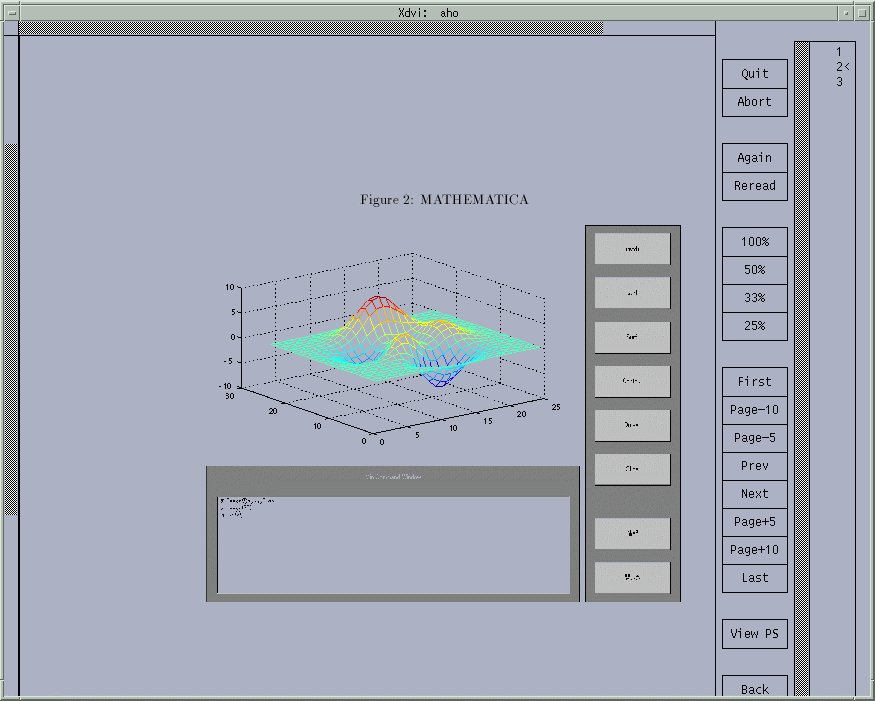
\includegraphics[bb={0 0 875 701},scale=.4]{images/xdvi}
%  \caption{{xdvi}の起動例}\figlab{xdvisample}
% \end{center}
%\end{figure}

\prog{xdvi}の基本的な操作方法を説明します.右側に枠で囲まれた
文字がボタンになっています.ボタンのように見えませんが一応押せます.
さらにボタンの右側にはページ番号があり,ページ番号をクリックすると
該当するページを表示します.

\prog{xdvi}でのマウスのクリックは拡大の機能を持っています.それぞれ
\begin{namelist}{中央クリック}
 \item[左クリック]   少し拡大.
 \item[中央クリック] 普通に拡大.
 \item[右クリック]   かなり拡大.
\end{namelist}
となっています.また,右側にある\qu{\str{Quit}}とか\qu{\str{Abort}}などは
ボタンで,主なボタンの機能は以下のとおりとです.
\begin{namelist}{View PS}
\item[\str{Quit}]
	    xdviを終了する.
\item[\str{Reread}]
	    一度読み込んだファイル\Va{file}{dvi}を再描画する.
\item[\str{First}]
	    先頭ページに移動する.
\item[\str{Prev}]
	    前ページに移動する.
\item[\str{Next}]
	    次ページに移動する.
\item[\str{Last}]
	    最終ページに移動する. 
\item[\str{View PS}]
	    {\PS}ファイルを見る.
\item[\str{File}]
	    DVIファイルを別に開く.
\end{namelist}

終了するには\qu{\str{Quit}}ボタンを押します. 


%\subsection{ちょっと休憩}
\begin{Trick}

これまで操作して少し疲れたでしょうから,ここで休憩をしましょう.
DVIファイルと言われてもなじみの薄いファイル形式かもしれません.
そこでこのDVIファイルを別のファイル形式に変換してみましょう.

例えば\PS に変換するには\pp{Windowsの方は\prog{dvipsk}}
\begin{InTerm}
  \type{dvips -o test.ps test.dvi}
\end{InTerm}
とすると\fl{test.dvi}から\fl{test.ps}が生成されます.この\fl{test.ps}を
\begin{InTerm}
  \type{ps2pdf test.ps test.pdf}
\end{InTerm}
としてPDFファイル\fl{test.pdf}を生成する事もできます.Postscript
ファイル\fl{test.ps}をプリンタに出力するには
\begin{InTerm}
  \type{lpr -P} \va{プリンタ名} \fl{test.ps}
\end{InTerm}
とする事で印刷要求を送信できます.\va{プリンタ名}については
システムの管理者に聞くなどしてください.

タイプセット時に拡張子\exten{tex}を省略して
\begin{InTerm}
  \type{platex test}
\end{InTerm}
としてみてください.以上のような例でも{\LaTeX}プログラムは
\fl{test.tex}を探し出してタイプセットしてくれるでしょう.

これは \LaTeX で使われているファイル検索の仕組みに関係しています.
\LaTeX では \Prog{Kpathsearch}というファイル検索機構を採用しています.
まず上記の例では\fl{test.tex}があるときに \type{platex test} とすると
\prog{Kpathsearch}が自動的に拡張子をつけてファイルを探します.
この時どのディレクトリ\pp{フォルダ}から探し出すかという情報が必要になりま
す.この情報が記載されたファイルは\Fl{texmf.cnf}というファイルです.
ほとんどの環境でディレクトリ \fl{\$texmf/web2c/} 以下にあります.%
\index{"$texmf@\texttt{\$texmf}}%
\index{ファイル!"$texmf@\texttt{\$texmf}}%
ここで \fl{\$texmf} は{\LaTeX}のファイルを格納すべき一番上のディレクトリを
示します.Unix系OSならば \fl{/usr/local/share/texmf/} 
などだったりWindowsならば \fl{C:\yen usr\yen local\yen share\yen 
texmf\yen} だったりするでしょう.
\begin{InTerm}
  \type{kpsewhich texmf.cnf}
\end{InTerm}
とすると,どこに\fl{texmf.cnf}が存在するのかが分かります.
\end{Trick}

\begin{Trick}
最近の \LaTeX プログラムは\prog{Kpathsearch}に対応しているので
何も意識しなくても適切に設定ファイルやクラスファイルなどを検索
してくれます.しかし手動で検索したいときもあると思います.
このような場合は\Prog{kpsewhich}というプログラムを使って
  \type{less `kpsewhich  book.cls`}
とすると\Fl{book.cls}というファイルが\fl{\$texmf}以下の
特定のディレクトリから検索され,\Prog{less}がファイルを
整形します.実はKpathsearch ではプログラム毎にファイルを
検索する場所を指定できます.そのため,\Fl{jarticle.cls}
というファイルを\type{kpsewhich jarticle.cls}としただけで
は検索結果に表示されません.\copt{-progname}というコマンドライン
オプションを付けて\type{kpsewhich -progname=platex jarticle.cls}
と実行すると,\pLaTeX が \Fl{jarticle.cls} というファイルを
見つけられる事になります.これにより複数のプログラムで同じ名前のファイル
名が存在しても,ディレクトリを変えておけば衝突しませんし,ファイルを検索
するディレクトリが少なくて済みますので処理速度が向上します.
\end{Trick}



\subsection{コマンド}

\zindind{原稿}{の構成}%
\zindind{原稿}{の先頭部分}%
{\LaTeX}では原稿を三つのパートに分割する事ができます.
それに伴いいくつかのコマンドは,特定のパートでしか使用
できません.
\begin{Syntax}
\verb|原稿先頭部分 (イニシャルコマンドを記述)|\\
\cmd{documentclass}\opa{オプション,$\ldots$}%
	\pa{クラス}\opa{リリース}\\
\va{前書き部分} (プリアンブルコマンドを記述)\\
\verb|\begin{document}|\\
\va{本文} (ボディ)\\
\verb|\end{document}|
\end{Syntax}
この中で \Cmd{documentclass},\Env{document}環境は必須であり,
絶対に必要な記述です.

\indindz{コマンド}{イニシャル}\indindz{コマンド}{プリアンブル}%
\zindind{プリアンブル}{コマンド}%
原稿先頭\pp{イニシャル}部分には\KY{イニシャルコマンド}と
呼ばれるコマンドを記述する事ができ,
同じように前書き\pp{プリアンブル}部分には%
\K{プリアンブルコマンド}や定義などを
記述する事ができます.そして,\env{document}環境
によって挟まれた本文部分にはコマンドの定義や組版用のコマンドを
記述します.それぞれのコマンドは定められた場所で使うように
決められています.ユーザがプリアンブルコマンドを本文で使う事が
できないように{\LaTeX}の内部で細工が施されています.

ここで言葉の定義をしましょう.コマンド,命令,環境,引数,オプションなど
の言葉を混同しがちですが,\K{本書では}以下のように取り決めます
\footnote{コマンドについての説明としては不十分なのですが,今は命令と環境
があると解釈してください.}.

\begin{description}%{コマンド}
\item[\Z{コマンド}] 
  \indindz{記号}{円}%
   \Z{バックスラッシュ}%
   \pp{Windowsの方は\Z{円記号}}と共に用いられる文字列.
   \begin{description}%{命令}
    \item[\Z{命令}]
       単独で使用するコマンド.
       引数を取る事ができる.
    \begin{quote}例:\verb|\alpha|,\verb|\maketitle|
          \end{quote}
    \item[\Z{環境}] 
       \qu{\C{begin}\pa{何々}}と
       \qu{\C{end}\pa{何々}}で囲まれている
     領域,またはそれを囲むためのコマンド.
       引数を取ることができる.
     \begin{quote}例:\verb|\begin{center}| \va{文字列} \verb|\end{center}|
    \end{quote}
   \end{description}
 \item[\Z{引数}] 
\zindind{コマンド}{の引数}%
\indindz{引数}{コマンドの}%
   コマンドに受け渡す文字列.
   \begin{description}%{必須引数}
    \item[\Z{必須引数}] 
\indindz{引数}{波括弧で挟まれた}%
\indindz{引数}{必須の}%
\zindind{波括弧}{で囲まれた引数}%
\zindind{波括弧}{の役割}%
       {波括弧}\qu{\texttt{\char'173~\char'175}}で囲まれた要素.
       コマンドが必須引数を取るときは必ず受け渡す.
           \begin{quote}例:\verb|\section|\pa{見出し語}\end{quote}
   \item[\Z{任意引数}] 
\indindz{引数}{角括弧で挟まれた}%
\indindz{引数}{任意の}%
\zindind{角括弧}{で囲まれた引数}%
       オプションとも言う.\Z{角括弧}\qu{\texttt{[~]}}で囲まれた要素.
       コマンドが任意引数を取るときは任意に受け渡す.
          \begin{quote}例:\verb|\documentclass|\opa{任意引数}\pa{クラス名}
    \end{quote}
   \end{description}
\end{description}
% commented out 2006/03/09 
%\begin{description}%{コマンド}
%\item[\Z{コマンド}] 
%	   \Z{バックスラッシュ}%
%	   \pp{Windowsの方は\Z{円記号}}と共に用いられる文字列.
%	   \begin{description}%{命令}
%	    \item[\Z{命令}]
%		       単独で使用するコマンド.
%		       引数を取ることができる.
%	    \begin{quote}例:\verb|\alpha|,\verb|\maketitle|
%            \end{quote}
%	    \item[\Z{環境}] 
%		       \qu{\Cmd{begin}\pa{なんとか}}と
%		       \qu{\Cmd{end}\pa{なんとか}}で囲まれている
%		       領域,またはそれを囲むためのコマンド.
%		       引数を取ることができる.
%            \begin{quote}例:\verb|\begin{center}文字列\end{center}|
%	    \end{quote}
%	   \end{description}
% \item[\Z{引数}] 
%	   コマンドに受け渡す文字列.
%	   \begin{description}%{必須引数}
%	    \item[\Z{必須引数}] 
%		       波括弧\qu{\texttt{\{\}}}で囲まれた要素.
%		       コマンドが必須引数をとるときは必ず受け渡す.
%            \begin{quote}例:\verb|\section{引数}|\end{quote}
%	    \item[\Z{任意引数}] 
%		       オプションとも言う.角括弧\qu{\texttt{[]}}で囲まれた要素.
%		       コマンドが任意引数をとるときは任意に受け渡す.
%            \begin{quote}例:\verb|\documentclass[任意引数]{jbook}|
%	    \end{quote}
%	   \end{description}
%\end{description}


\subsection{括弧について}

%さて,{\LaTeX}の基本を知った所で\KY{括弧}に
%ついての取決めをしたいと思います.括弧については色々な呼
%び方があるようですが,誤解を避けるために\K{本書では}
%以下のように定義します.
%\begin{description}
% \item[\Z{かぎ括弧} \qu{「」}] 
%	    引用や会話文などに使う.
% \item[\Z{2重かぎ括弧} \qu{『』}] 
%	    書名,引用の中の引用などに使う.
% \item[\Z{引用符} \qu{‘’}] シングルクオートとも言う.左側に
%	    あるほうを左シングルクオート,右側にあるほうを
%	    右シングルクオートと言う.引用に使う.
% \item[\Z{2重引用符} \qu{“”}] 
%	    ダブルクオートとも言う.左側にあるほうを左ダブルクオート,
%	    右側にあるほうを右ダブルクオートという.
%	    長い引用に使う.
% \item[\Z{丸括弧} \qu{()}] 小括弧,パーレンとも言う.
%	    語句の補足説明に使う.
% \item[\Z{波括弧} \qu{{}}] 中括弧とも言う.
%	    コマンドに対して必須引数を渡すのに
%	    使われたり,要素を一つのグループにまとめるために
%	    使う.
% \item[\Z{角括弧} \qu{[]}] 大括弧とも言う.
%	    コマンドに対して任意引数を渡すときに使う.
% \item[\Z{山括弧} \qu{<>}] 
%	    この括弧に囲まれた文字列は何か別の文字列に
%	    書き換えられる.例えば,\va{ファイル名}などがあれば,
%	    これは任意の文字列\fl{filename.tex},
%	    \fl{test.foo}などに置き換えられる.
%\end{description}
%ここで引用符と言うのが登場しましたが,欧文の引用符は
%シングルクオート\pp{`'}であり,和文の引用符はかぎ括弧\pp{「」}と
%なります.二つを区別するために欧文用のものを
%\K{シングルクオート},和文のものを\K{かぎ括弧}と言う
%ことにします.文中に出てくる引用符という言葉は
%そのどちらも示すことになります.
さて,{\LaTeX}の基本を知った所で\KY{括弧}に
ついての取決めをしたいと思います.括弧については色々な呼
び方があるようですが,誤解を避けるために\K{この冊子では}
以下のように定義します.
\begin{description}
 \item[\Z{かぎ括弧}---「~」] 
	    \Z{引用}や\Z{会話文}などに使う.
 \item[\Z{二重かぎ括弧}---『~』] 
	    \Z{書名},引用の中の引用などに使う.
 \item[\Z{引用符}---‘~’] シングルクオートとも言う.左側に
	    あるほうを左シングルクオート,右側にあるほうを
	    右シングルクオートと言う.引用に使う.
 \item[\Z{二重引用符}---“~”] 
	    ダブルクオートとも言う.左側にあるほうを左ダブルクオート,
	    右側にあるほうを右ダブルクオートという.
	    長い引用に使う.
 \item[\Z{丸括弧}---(~)] \Z{小括弧},\Z{パーレン}とも言う.
	    語句の\Z{補足説明}に使う.
 \item[\Z{波括弧}---{~}] \Z{中括弧}とも言う.
	    コマンドに対して必須引数を渡すのに
	    使われたり,要素を一つのグループにまとめるために
	    使う.
 \item[\Z{角括弧}---[~]] \Z{大括弧}とも言う.
	    コマンドに対して任意引数を渡すときに使う.
 \item[\Z{山括弧}---<~>] 
	    この括弧に囲まれた文字列は何か別の文字列に
	    書き換えられる.例えば,\va{ファイル名}などがあれば,
	    これは任意の文字列\fl{file.tex},
	    \fl{input.foo},\fl{output.bar}などに置き換えられる.
\end{description}
\indindz{引用符}{欧文の}%
\indindz{引用符}{和文の}%
\zindind{欧文}{の引用符}%
\zindind{和文}{の引用符}%
ここで\Z{引用符}と言うのが登場しましたが,欧文の引用符は
シングルクオート\pp{`~'}であり,和文の引用符はかぎ括弧\pp{「~」}と
なります.二つを区別するために欧文用のものを
\KY{シングルクオート},和文のものを\KY{かぎ括弧}と言う
ことにします.文中に出てくる引用符という言葉は
そのどちらも示すことになります.


\section{{\protect\LaTeX}に関わるファイル形式}
タイプセット時に作成される中途ファイル以外にも{\LaTeX}では多く
のファイル形式が存在することを経験するでしょう.一般にファイ
ル形式は\KY{拡張子}によって種類を識別します.

\begin{Syntax}
\Va{ファイル名}{拡張子}
\end{Syntax}

上記のようにピリオドの後の文字で区別されます.

パッケージをインストールするときに見かけるものは以下の通りです.
\begin{namelist}{xxxx}
%\item[\Exten{dtx}] パッケージ化されたマクロ.複数のクラス
%\Va{クラス1}{cls},\Va{クラス2}{cls},\ldots\, \Va{クラスn}{cls}が
%\Va{クラス}{dtx}中にまとまっていることも多い.または
%\Va{マクロ}{sty}が複数まとまっているときもある.
%\item[\Exten{ins}] パッケージ化されたマクロを
%    取り出すためのファイル.\Va{classes}{dtx}と
%    ともに配布されている.
%\item[\Exten{sty}] 便利な機能をうまくまとめたもの.
%    \emph{マクロ},\emph{マクロパッケージ},\emph{パッケージ},
%    \emph{スタイルファイル}\pp{ちと古い言い方}とも言う.
%\item[\Exten{cls}] 原稿の書式を決定するファイル.
%    \emph{クラス},\emph{クラスファイル},\emph{文書クラスファイル},
%    \emph{ドキュメントクラスファイル}とも言う.
%\item[\Exten{clo}] クラスのオプションに応じた設定を記述したファイル.
%\item[\Exten{fd}]  フォントの属性を定義したファイル.ユーザが意識して
%		    使うことはない.
\indindz{マクロ}{パッケージ化された}%
\item[\Exten{dtx}] パッケージ化されたマクロ.複数のクラス
\Va{クラス1}{cls},\Va{クラス2}{cls},\ldots\, \Va{クラスn}{cls}が
\Va{クラス}{dtx}中にまとまっていることも多い.または
\Va{マクロ}{sty}が複数まとまっているときもある.
\item[\Exten{ins}] パッケージ化されたマクロを
    取り出すためのファイル.\Va{classes}{dtx}と
    ともに配布されている.
\item[\Exten{sty}] 便利な機能をうまくまとめたもの.
    \KY{マクロ},\KY{マクロパッケージ},\KY{パッケージ},
    \KY{スタイルファイル}とも言う.
\item[\Exten{cls}] 
\indindz{書式}{原稿の}%
\zindind{原稿}{の書式}%
\zindind{クラス}{ファイル}%
\indindz{ファイル}{文書クラス}%
\indindz{ファイル}{ドキュメントクラス}%
  原稿の\Z{書式}を決定するファイル.
  \KY{クラス},\K{クラスファイル},\K{文書クラスファイル},%
  \zindind{ドキュメントクラス}{オプション}%
  \K{ドキュメントクラスファイル}とも言う.
\item[\Exten{clo}] 
  クラスのオプションに応じた設定を記述したファイル.
\item[\Exten{fd}]  
  \zindind{書体}{の属性}%
  書体の属性を定義したファイル.ユーザが意識して使うことはない.
\end{namelist}

原稿を作成するときに見かけるものは以下の通りです.
\begin{namelist}{xxxx}
\item[\Exten{tex}] 
  {\LaTeX}が処理を受け付ける原稿.\KY{ソース},\KY{ソースファイル}とも言う.
\item[\Exten{bib}] 
  文献成形プログラム{\BibTeX}が処理できる参考文献ファイル.
  \K{参考文献データベース}と言う.
\item[\Exten{bst}] 
  参考文献の表示形式を決めるもの.\K{参考文献スタイル}と言う.
  \indindz{スタイル}{参考文献}%
\item[\Exten{eps}] 
 Adobe社が開発したページ記述言語{\PS}で書かれたファイル.
 \zindind{画像}{ベクトル}%
 主に単一ページのベクトル画像などに使われる.\zindind{ページ}{記述言語}
\item[\Exten{ist}] 
 索引の書式を決めるファイル.\K{索引スタイル}と言う.\indindz{スタイル}{索引}%

\end{namelist}

原稿をタイプセットした後に見かけるものは以下の通りです.
これらは全て中途ファイルであり,{\LaTeX}が原稿を完成させるた
めに必要なものです.
\begin{namelist}{xxxx}
\item[\Exten{log}] {\LaTeX}の組版結果の詳細情報.
		    \KY{ログファイル}と言う.
\item[\Exten{aux}] 相互参照などの情報が書かれたファイル.
		    1度目以降の処理に必要とされる.
\item[\Exten{dvi}] 原稿を{\LaTeX}でタイプセットした後に作成される
		    印刷結果に限りなく近いファイル.このファイルを
		    プレビューしたり,または他の{デバイスドライバ}%
		    によって別の形式に変換できる.
\item[\Exten{toc}] \zindind{目次}{用の中途ファイル}
    \yo{目次}を出力するための目次情報が書き出されたファイル.
\item[\Exten{lof}] 
    \yo{図目次}を出力するための図目次情報が書き出されたファイル.
\item[\Exten{lot}] 
    \yo{表目次}を出力するための表目次情報が書き出されたファイル.
\item[\Exten{bbl}] {\BibTeX}によって並べ替えをした後の
    参考文献リスト.\Env{thebibliography}環境を用いて記述されている.
\item[\Exten{blg}] {\BibTeX}の実行結果が出力されるログファイル.
\item[\Exten{idx}] 並べ替えられる前の索引の語句が書き出されたファイル.
    \Prog{MakeIndex},\Prog{mendex}などの
    プログラムで並べ替えをする.
\item[\Exten{ind}] \prog{makeindex}などによって
    並べ替えられた索引ファイル.標準的には\Env{theindex}
    環境を用いて記述されている.
\item[\Exten{ilg}] \prog{makeindex}などを実行したときの処理結果が
   出力されるログファイル.
\end{namelist}

その他画像形式に関わる拡張子として,主に以下のものがあります.
\indindz{画像}{フルカラー}%
\indindz{画像}{無圧縮}%
\indindz{画像}{可逆圧縮}%
\indindz{ビットマップ画像}{フルカラー}%
\indindz{ビットマップ画像}{無圧縮}%
\indindz{ビットマップ画像}{可逆圧縮}%
\begin{namelist}{jpeg}
\item[\Exten{jpg}] 
  写真などのフルカラーに適したビットマップ画像.
\item[\Exten{bmp}] 
  Windows 標準の無圧縮ビットマップ画像.
\item[\Exten{png}]
  可逆圧縮で\prog{\Dvipdfm}が標準で対応しているビットマップ画像.
\item[\Exten{bb}]
  \LaTeX が画像のバウンディングボックス情報を得るために必要とする
  ファイル.\Prog{ebb}や\Prog{CreateBB}で作成できる.
\item[\Exten{mp}] 
  \Prog[MetaPost]{\MP}で描画された\Z{ベクトル画像}.
\end{namelist}


\section{コマンドの基本}
{\LaTeX}では便利なコマンドがあらかじめ用意されています.
それらをどのように用いるか,また必要な機能がないときは
どうすれば良いのかを説明します.

\subsection{原稿の先頭でのコマンド}
\zindind{原稿}{のプリアンブル}%

少し前置きが長くなりましたが{\LaTeX}の原稿の構造をもう一度
見ておきましょう.
\begin{Syntax}
\cmd{documentclass}\opa{オプション,\,$\ldots$}%
	\pa{クラス}\opa{リリース}\\
\va{前書き部分} (プリアンブルコマンド)\\
\verb|\begin{document}|\\
\va{本文} (ボディ)\\
\verb|\end{document}|
\end{Syntax}
\zindind{原稿}{の先頭}%%
さて,原稿の先頭部分,\cmd{documentclass}が始まる前の
イニシャルコマンドには\Env{filecontents}環境が使えます.
\begin{Syntax}
\verb|\begin{filecontents}|\pa{ファイル名}\\
\va{内容}\\
\verb|\end{filecontents}|
\end{Syntax}
この\env{filecontents}環境が持つ機能ですが,指定した
\va{ファイル名}に\va{内容}を書き出してくれます.
例えば原稿を一つのファイルとしてしか配布できない場合に
EPS画像などを同時に含めるならば,この部分にEPS画像の
ソースを記述します.ただしこの環境は書き出すファイル
の先頭にコメントを挿入しますので,アスタリスク\qu{\str*}を
付けると自動的に付加される余分なコメントが入りません.

\begin{InTeX}
\begin{filecontents*}{<ファイル名>}
%!PS-Adobe-2.0なんとかかんとか...
\end{filecontents*}
\end{InTeX}


\subsection{プリアンブルでのコマンド}
原稿の先頭には\env{filecontents}環境が使えることは分かりました.次に書く
べきコマンドは \C{documentclass} 命令です.
\begin{Syntax}
\cmd{documentclass}\opa{オプション,\,$\ldots$}\pa{クラス名}\opa{リリース}
\end{Syntax}
この命令は\yo{これから文書で使う命令の定義や前書きを
書きます}という意味合いを持っており,
この命令を書いた後は原稿の\Z{前書き部分}
\pp{\Z{プリアンブル}}として解釈されます.

\va{クラス名}には\secref{01pregame:sec:classes}で
紹介するものが使えます.\va{オプション}にはそれぞれの
クラスが用意している任意引数を渡すことができます.
このオプションのことを特に\K{文書クラスオプション}とか%
\zindind{ドキュメントクラス}{オプション}%
\zindind{文書クラス}{オプション}%
\K{ドキュメントクラスオプション}と言います.
\va{リリース}には自分の使っているクラスファイルが
いつ配布されたのかを書きます.

\va{リリース}にはクラスの配布された日付を\va{YYYY/MM/DD}
という書式で記述できます.例えば,2003年12月31日に公開された
日本語のクラス\Cls{jarticle}ならばおおむね以下のようになります.

\begin{InTeX}
\documentclass[11pt,a4j]{jarticle}[2003/12/31]
\end{InTeX}

もしも,クラスファイルが2003年12月31日以前のもので
要求されているバージョンよりも古ければ,
{\LaTeX}はタイプセット時に次のような\Z{警告}\pp{\Z{warning}}を出します.

\index{You have requested, on input line n@\texttt{You have requested, on input line n}}%
\index{警告!You have requested, on input line n@\texttt{You have requested, on input line n}}%
\begin{OutTerm}
LaTeX Warning: You have requested, on input line 1, version
               `2003/12/31' of document class jarticle,
               but only version
               `2002/04/09 v1.4 Standard pLaTeX class'
               is available.
\end{OutTerm}

他にも\secref{01pregame:sec:stdmacro}で紹介しているような
パッケージを使う場合はプリアンブル部分に \Cmd{usepackage} を
使います.
\begin{Syntax}
\cmd{usepackage}\opa{オプション,\,$\ldots$}%
 \pa{パッケージ名}\opa{リリース}
\end{Syntax}
これはプリアンブルのみでしか使えません.
\cmd{usepackage}命令は \cmd{documentclass}命令と同じように,
そのパッケージが提供するオプションを指定したり,リリースには
そのパッケージのバージョンを指定できます.
\zindind{デバイス}{ドライバ}%
例えば,画像ファイルなどを{\LaTeX}で扱いたいと思い,
デバイスドライバとして\prog{\Dvipdfmx}を使う場合は
次のように\str{graphicx}パッケージを使うことを\K{プリアンブルで}
宣言します.

\begin{InTeX}
\usepackage[dvipdfmx]{graphicx}[2001/01/01]
\end{InTeX}

同じパッケージを2度や3度以上読み込もうとしても,
1度読み込まれているなら再度読み込もうとしません.
パッケージに渡すオプション\pp{リリースを除く}を特に
\zindind{パッケージ}{オプション}\K{パッケージオプション}
と呼びます.

文書クラスオプションやパッケージオプションのいずれにしても,
たいてい\yo{命令}と\yo{必須引数}のあいだの\va{オプション}\pp{任意引数}
は\K{複数個渡すことができます}.

\begin{InTeX}
\documentclass[10pt,a4paper,twocolumn]{article}
\end{InTeX}

例えば\option{10pt},\option{a4paper},\option{twocolumn}と
いう三つのオプションは\Z{コンマ}\qu{\str,}を区切りとして書けば良いのです.

同時に複数のパッケージを使うことも宣言できます.
\sty{graphicx},\sty{amsmath},\sty{makeidx}などを
次のように宣言できますが,そうするとパッケージオプションをそれぞれのパッ
ケージに対して渡すことはできません.

\begin{InTeX}
\usepackage{graphicx,amsmath,makeidx}
\end{InTeX}

基本的なソースファイルの構成は次のようになります.

\begin{InTeX}
\documentclass[a4j]{jarticle} 
\usepackage[dvipdfmx]{graphicx}
\usepackage[dvipdfmx,usenames]{color}
\begin{document}
ここに文章を記述します.
\end{document}
\end{InTeX}

\begin{Trick}
 後述のデバイスドライバの指定に関しては,上記のような
 記述ではなく,ドキュメントクラスオプションに,使用する
 デバイスドライバを追加するのが安全です.

\begin{InText}
\documentclass[dvipdfmx,a4j]{jarticle} 
\usepackage{graphicx}
\usepackage[usenames]{color}
\end{InText}

これによりドキュメントクラスオプションが\KY{グローバルオプション}
としての機能を果たし,\cmd{usepackage}で読み込まれるマクロパッケージ
全てに渡される事になります.
\end{Trick}


{\LaTeX}処理を実行した原稿のプリアンブルに以下を記述します.

\begin{Syntax}
\cmd{listfiles}
\end{Syntax}

\Cmd{listfiles}命令を記述すれば,自分が処理している
原稿に何のファイルが使用されているのかを端末と
\Va{file}{log}に書き出します.

\begin{Prob}
実際に以下のファイル\Fl{listfile.tex}を作成,タイプセットしてください.

\begin{InTeX}
\documentclass{jbook}
\listfiles
\begin{document}
 test 
\end{document}
\end{InTeX}

%\prog{platex}でタイプセットしたならば次のような表示が出るでしょう.

%\begin{OutTerm}
%This is pTeX  Version 3.141592-p3.1.2 (sjis)(Web2C 7.5.2) 
% *File List*
%  pldefs.ltx    2000/07/13 v1.2 pLaTeX Kernel
%   jy1mc.fd    1997/01/24 v1.3 KANJI font defines
%   jy1gt.fd    1997/01/24 v1.3 KANJI font defines
% kinsoku.tex
% plpatch.ltx
%   jbook.cls    2001/10/04 v1.3 Standard pLaTeX class
%   jbk10.clo    2001/10/04 v1.3 Standard pLaTeX file
% ***********
%Output written on listfile.dvi (1 page,216 bytes).
%Transcript written on listfile.log.
%\end{OutTerm}
\begin{comment}
\begin{OutTerm}
This is pTeX, Version 3.14159-p3.1.5 (euc) (Web2C 7.4.5)
(./filetest.tex
pLaTeX2e <2005/01/04>+0 (based on LaTeX2e <2001/06/01> patch level 0)
(/usr/local/share/texmf/ptex/platex/base/jarticle.cls
Document Class: jarticle 2002/04/09 v1.4 Standard pLaTeX class
(/usr/local/share/texmf/ptex/platex/base/jsize10.clo)) 
(./filetest.aux) [1] (./filetest.aux)

 *File List*
  pldefs.ltx    2000/07/13 v1.2 pLaTeX Kernel (Default settings)
   jy1mc.fd    1997/01/24 v1.3 KANJI font defines
   jy1gt.fd    1997/01/24 v1.3 KANJI font defines
   jt1mc.fd    1997/01/24 v1.3 KANJI font defines
   jt1gt.fd    1997/01/24 v1.3 KANJI font defines
 kinsoku.tex
 plpatch.ltx
jarticle.cls    2002/04/09 v1.4 Standard pLaTeX class
 jsize10.clo    2002/04/09 v1.4 Standard pLaTeX file (size option)
 ***********

)
Output written on filetest.dvi (1 page, 216 bytes).
Transcript written on filetest.log.
\end{OutTerm}
\end{comment} 

出力結果からどのような事が分かるでしょうか.
ここで少し疑問に思っていただきたいことは,\yo{原稿には\Cls{jbook}を使う
ことしか宣言していないのに何か別のファイルも一緒に読み込まれている}と
いうことです.この例では\Fl{pldefs.ltx}をはじめとして,\Fl{kinsoku.tex}
や\Fl{jsize10.clo}等のファイルが読み込まれています.
\end{Prob}


\section{執筆環境における基本}\seclab{basic:lakulaku}
\zindind{原稿}{作成の支援}%

\TeX はテキストエディッタによって原稿を執筆するという方法を取るため,何ら
かの執筆環境を必要とします.それらの執筆環境の中には作業の簡略化を目的と
したものも数多くあります.
\TeX における伝統的な (\Z{obsolete}) \Z{執筆環境}には次のようなものが
挙げられます.
\begin{description}
 \item[\unixos] 
 \TeX とその周辺のプログラムを活用しようと思えば,\unixos
 を使うと(人によっては)快適な執筆環境を得る事ができます.\Prog{Vine Linux}は特に \TeX 周辺
 の日本語環境が整っていると思われます\footnote\webVineLinux .
 \item[\Prog{Emacs}] 
 \LaTeX の原稿となるソースファイルを編集する時に役に立つテキストエディッタです.
 \item[{\Prog[yatex]\YaTeX}]
 上記Emacs上で動作する\Hito{広瀬}{雄二}\footnote\webYaTeX による \LaTeX
 執筆支援システムです.
 \item[\Prog{Tgif}] 
 \zindind{画像}{編集}%
 \unixos で広く使われているベクター画像編集プログラムです.
  \item[\Prog{Gnuplot}] 
 \unixos で広く使われているグラフを描画したり,データをプロットするため
 のプログラムです.
 \item[\Prog{Make}]
  \zindind{原稿}{の再コンパイル}%
  原稿の再コンパイルを支援するためのプログラムです.\Fl{Makefile}とい
  う特別なファイルを用意する事で,再コンパイルにおける手間を軽減する事に
  なります.
\end{description}

環境に依存してはいるものの,以下に挙げるように \LaTeX での煩雑な作業を軽
減できる有益な原稿執筆支援環境が数多く存在します.
\begin{description}
\zindind{Windows}{の執筆支援環境}%
% \item[\Prog{WinShell} (Windows)]
% \Person{Ingo H. de}{Boer}らによる統合執筆支援環境です\footnote
% \webWinShell .コマンドラインから
% の煩雑な操作なしにタイプセット等ができるようになります.
 \item[{\Prog[EasyTeX]{Easy\TeX}}] \Hito{中川}{仁}によるWindows用の執
 筆支援環境です\footnote\webEasyTeX .
 \LaTeX に慣れないうちはEasy\TeX を使うのが望ましいでしょう.
 導入方法や操作方法に関しては\Hito{大友}{康寛}による解説%
 \footnote{\url{http://www.klavis.info/etexinst.html}}や
 \TeX~Wiki\footnote{\url{http://cise.edu.mie-u.ac.jp/~okumura/texwiki/?EasyTeX}}%
 等を参照してください.


\zindind{Mac OS X}{の執筆支援環境}%
 \item[{\Prog[TeXShop]{\TeX Shop}}] 
  Mac~OS~X で使用できる\Person{Richard}{Koch}らによる執筆支援環境で
  す\footnote{\webTeXShop}.PDF でのプレビューが可能でディスプレイにおけ
  る表示がきれいです.
\end{description}

基本的にフリーウェアで済ませたいので,上記のような選択肢になる人も
多い事でしょう.Easy\TeX や \TeX Shop ではコマンドの入力を補完
したり,プログラムの実行等も簡単にできる環境が整備されています.
まず最初はこのようなプログラムを使った執筆の方が負荷も少ないと思われます.

もちろん,シェアウェアの方がサポートもありますし,バージョンアップも確実
な部分があると思います.いずれにしてもその人にとって適切だと思われるツー
ルは多少なりとも異なると思われますので,いくつか試用してみてください.

%#!platex jou.tex
\section{���Ƥν��Ϸ���}
%\begin{abstract}
%{\LaTeX}�θ��Ƥμ�ɮ������ä��餽�������\pp{�����ץ��å�}
%���ʤ���Фʤ�ʤ��Τϼ����Τ��ȤǤ������ɤΤ褦��
%�ե���������ˤ��뤫�����Ӥˤ��ʬ�����Ȥ����Ǥ���
%���ξϤǤϤɤΤ褦�ʥե��������������Τ����ɤ���ä�
%�Ѵ�����Τ����������ޤ���
\zindind{����}{�ν��Ϸ���}%
{\LaTeX}�θ��Ƥμ�ɮ������ä��餽�������\pp{�����ץ��å�}���ʤ���Ф�
��ʤ��Τϼ����λ��Ǥ������ɤΤ褦�ʥե���������ˤ��뤫�����Ӥˤ�ä�
ʬ�����Ȥ����Ǥ���������ǤϤɤΤ褦�ʥե��������������Τ����ɤ����
���Ѵ�����Τ����������ޤ���
%\end{abstract}

\subsection{���Ϸ����μ���γ���}

{\LaTeX}�θ��Ƥμ�ɮ������ä��餽�������\pp{�����ץ��å�}���ʤ���Ф�
��ʤ��Τϼ����λ��Ǥ������ɤΤ褦�ʥե���������ˤ��뤫�����Ӥˤ��ʬ
�����Ȥ����Ǥ�����Ū�ȵ�ʬ�ˤ�äƤ��η������Ѥ��ޤ��������줾��η�����
�ɤΤ褦����ħ����äƤ���Τ����ΤäƤ����ʤ���С��ɤη������Ѵ������
�ɤ��Τ���ʬ����ޤ��󡥤Ǥ�����ޤ��ϤɤΤ褦�ʷ�����¸�ߤ����ɤΤ褦��
��ħ������Τ���Ҳ𤷤ޤ���

\begin{description}
%\item[DVI]
%  DVI��\emph{Device Independent}��ά�����֤˰�¸���ʤ�
%  ���ѤΥڡ������Ҹ���Ǥ���������ޤ�����ü��
%  �����ԤäƤ��ʤ����Ƥξ��Ϥ���DVI�ե����뤫��
%  ������Ԥ����Ȥ��Ǥ��ޤ������֤˰�¸����̿���
%  ����DVI�ե��������˵��Ҥ���Ƥ��ꡤ�����Ŭ�ڤ�
%  ��ᤷ�Ƥ����ǥХ����ɥ饤�Ф�����ޤ����̾��
%  �ץ�ӥ塼����Ѥ˻Ȥ��Ƥ��ޤ���DVI�ե������
%  \Va{file}{dvi}�Τ褦�˳�ĥ�Ҥ�\exten{dvi}�Ȥʤ�ޤ���
%\item[{\PS}]
%  Adobe�Ҥ��Τ˳�ȯ�����ڡ������Ҹ���Ǥ���
%  ���ߤΥС�������1.3��Unix��OS�ǤϤ���{\PS}������
%  �ե����뤬�ץ�ӥ塼�ڤӰ����˹����Ȥ��Ƥ��ޤ����ɤ�
%  {\PS}���ά����PS�Ƚ񤯤��Ȥ�����ޤ�������ĥ�Ҥ�
%  \exten{ps}�ˤʤäƤ��ޤ���ɸ��Ǥ�  �ե����뤬���̤���
%  �ʤ��Τ�\Va{file}{ps.gz}�η������ۤ���Ƥ��뤫�⤷���
%  ���󡥰����ȳ��Ǥ⤳��{\PS}  �������ɤ��Ȥ��Ƥ�
%  �ޤ���{\PS}����֤�EPS\pp{Encapsulated {\PS}}
%  �Ȥ����ե���������⤢��ޤ���������ϥ٥��ȥ������
%  �ɤ��ɤ��Ȥ��Ƥ��ޤ���
%\item[PDF]
%  PDF��Portable Document Format��ά��Adobe�Ҥγ�ȯ���Ƥ���
%  {\PS}�θ�ѤΥڡ������Ҹ���Ǥ���\zindind{�ڡ���}{���Ҹ���}
%  ���ߤΥС�������1.5�ǥץ�ӥ塼�Ȱ�����̤�Ʊ���٤��ʼ�
%  �����뤳�Ȥ��Ǥ�������Ǥ���������ǹ����Ȥ��Ƥ��ޤ���
%  ���ܸ���̤�ޤ���{\LaTeX}�����θ��Ƥ�ľ��PDF���Ѵ�����
%  \Prog[pdfLaTeX]{pdf\LaTeX}�Ȥ����ץ�������¸�ߤ��ޤ���
%\item[HTML]
%  \Z{HTML} HyperText Markup Language��ά�ǥ����־��
%  �����������뤿���\Z{�ϥ��ѡ����} 
%  \pp{\Z{Hyper Link}}�Ȥ�����ǽ���������ڡ������Ҹ���Ǥ���
%  ���ʥ����֥֥饦�����鸫�Ƥ���ڡ�����HTML�ǵ��Ҥ����
%  ���ޤ������ߤ�HTML�θ�Ѥ�XHTML����ή�ˤʤ����Ȥ��Ƥ��ޤ���
%  {\LaTeX}��Ʊ���褦��\Z{�ޡ������å�}����Ǥ���
\item[DVI]
  \indindz{̿��}{���֤˰�¸����}%
  \indindz{̿��}{�ǥХ�����¸��}%
  DVI��\emph{Device Independent}��ά�����֤˰�¸���ʤ�
  ���ѤΥڡ������Ҹ���Ǥ���������ޤ�����ü��
  �����ԤäƤ��ʤ����Ƥξ��Ϥ���DVI�ե����뤫��
  ������Ԥ������Ǥ��ޤ������֤˰�¸����̿���
  ����DVI�ե��������˵��Ҥ���Ƥ��ꡤ�����Ŭ�ڤ�
  ��ᤷ�Ƥ����ǥХ����ɥ饤�Ф�����ޤ����̾��
  �ץ�ӥ塼����Ѥ˻Ȥ��Ƥ��ޤ���DVI�ե������
  \Va{file}{dvi}�Τ褦�˳�ĥ�Ҥ�\Exten{dvi}�Ȥʤ�ޤ���
\item[{\PS}]
  \zindind{�ڡ���}{���Ҹ���}%
  Adobe�Ҥ��Τ˳�ȯ�����ڡ������Ҹ���Ǥ���
  ���ߤΥС�������1.3��\unixos �ǤϤ���{\PS}������
  �ե����뤬�ץ�ӥ塼�ڤӰ����˹����Ȥ��Ƥ��ޤ����ɤ�
  {\PS}���ά����PS�Ƚ񤯻�������ޤ�������ĥ�Ҥ�
  \Exten{ps}�ˤʤäƤ��ޤ���ɸ��Ǥ�  �ե����뤬���̤���
  �ʤ��Τ�\Va{file}{ps.gz}�η������ۤ���Ƥ��뤫�⤷���
  ���󡥰����ȳ��Ǥ⤳��{\PS}  �������ɤ��Ȥ��Ƥ�
  �ޤ���{\PS}����֤�EPS\pp{Encapsulated {\PS}}
  �Ȥ����ե���������⤢��ޤ����������ñ��ڡ���������
  �ɤ��ɤ��Ȥ��Ƥ��ޤ���\indindz{����}{ñ��ڡ�����}
\item[PDF]
\zindind{PDF}{�ΥС������}%
  PDF��Portable Document Format��ά��Adobe�Ҥγ�ȯ���Ƥ���
  {\PS}�θ�ѤΥڡ������Ҹ���Ǥ���\zindind{�ڡ���}{���Ҹ���}
  \genzai �κǿ��С�������1.6�ǡ�
  �ץ�ӥ塼�Ȱ�����̤�Ʊ���٤��ʼ�����������Ǥ�������Ǥ����ߴ�����
  ��θ����ХС������� 1.3 �����줹��Τ�̵����Ȼפ��ޤ���PDF ����
  ����ǹ����Ȥ��Ƥ��ޤ���\genzai �����ܸ첽�Ϥ���Ƥ��ޤ��󤬡�
  {\LaTeX}�����θ��Ƥ�ľ�� PDF���Ѵ����� \Prog[pdfLaTeX]{\PDFLaTeX}�Ȥ�
  ���ץ�������¸�ߤ��ޤ���\zindind{����}{����PDF�κ���}%
\item[HTML]
  \Z{HTML} HyperText Markup Language��ά�ǥ����־��
  �����������뤿���\Z{�ϥ��ѡ����} 
  \pp{\Z{Hyper Link}}�Ȥ�����ǽ���������ڡ������Ҹ���Ǥ���
  ����\Z{�����֥֥饦��}���鸫�Ƥ���ڡ�����HTML�ǵ��Ҥ����
  ���ޤ������ߤ�HTML�θ�Ѥ�XHTML����ή�ˤʤ����Ȥ��Ƥ��ޤ���
  {\LaTeX}��Ʊ���褦��\Z{�ޡ������å�}����Ǥ���
\end{description}
�ʾ�η����Τۤ��ˤ⤢��ΤǤ�����ͭ̾�ʷ����Ϥ��λͤĤǤ���
���߹����Ѥ����Ƥ���Τ�PDF�����Ǥ����顤�ܽ�Ǥ�PDF�Ȥ��μ��դ˴ؤ�
�ƾܤ������⤷�ޤ���

%���ξϤǤϤɤΤ褦��{\LaTeX}�θ��Ƥ�Ʒ������Ѵ����뤫����⤷�ޤ���

\subsection{\LaTeX �θ��Ƥ���DVI��}
\Z{DVI}�Ȥ�\emph{DeVice Independent}��ά�ǥǥХ����˰�¸���ʤ��ե������
���Ǥ����̾�{\LaTeX}��������η�̤�ޤȤ��Τ⤳��DVI�����Ǥ���
\prog{platex}�ʤɤΥץ�������{\LaTeX}�θ��Ƥ򥳥󥽡��뤫�鼡�Τ褦��
����С�\LaTeX �θ��ƥե����� \Va{filename}{tex} ����DVI�ե�����
\Va{filename}{dvi} ����������ޤ���

\begin{InTerm}
   \type{platex filename.tex}
\end{InTerm}

���ΤȤ��̾�ϥ��������ˤ�ä����ܸ첽���줿 \pLaTeX ���Ѥ��ޤ�
\footnote{���������Υץ������Ȥ��̤�NTT�ˤ�ä����ܸ첽���줿\JLaTeX
��¸�ߤ��ޤ���}��

�ߴ����ΰ٤ˡ��Ť�\LaTeX��\LaTeX\,2.09 ����Υ������ե�����򥿥��ץ���
�Ȥ���ˤ� \prog{platex209}���ޥ�ɤ�Ȥ��ޤ���

\begin{InTerm}
 \type{platex209 oldfile.tex}
\end{InTerm}

\latexno{���}%
\indindz{�ե�����}{��������}%
\zindind{����}{����Ƭ}
�ز����ˤ�äƤ�\LaTeXe
���б����Ƥ��ʤ��Ť��񼰤Υ��饹�ե������\Z{��������ե�����}�����󶡤���
���ʤ���礬����ޤ���\LaTeXe �� \LaTeX\,2.09 ��ʬ������ˡ�ϴ�ñ�Ǥ���
\LaTeX �θ��� \Va{file}{tex}����Ƭ��̿������ܤ��ޤ���

\begin{itemize}
 \item \Cmd{documentclass} ̿���ȤäƤ���� \LaTeXe �ѤΥե����롥
 \item \Cmd{documentstyle} ̿���ȤäƤ���� \LaTeX\,2.09 �ѤΥե����롥
\end{itemize}

\LaTeX\,2.09����ξ��ϡ�\cmd{usepackage}̿��ϻȤ��ޤ��󡥤��Τ��ᡤ
\cmd{documentstyle}��Ǥ�հ�����ɬ�פȤ��륹������ե��������󤷤ޤ���

\begin{InTeX}
 \documentstyle[url,mysetting,...]{jarticle}
\end{InTeX}

�ä��ᤷ�ƥ����ץ��åȸ�����������DVI�ե�����ˤϥ���դ�����ʤɤο�
����������Ƥ��ޤ��󤬡������ξ����DVI�ե�����˵��ܤ���Ƥ��ޤ�����
�ʤɤ����̤ʾ������Ǥ��뤫�Ϥ���\K{�ץ�ӥ塼����ǥХ����ɥ饤�Ф�
��¸���Ƥ��ޤ�}��

%DVI�ե�����ϥץ�ӥ塼�ʤɤǰ��Ū�����Ǹ�η�̤��ǧ����Τ������Ǥ���
%Windows�Ǥ�\Hito{����}{��ͺ}�餬��ȯ���Ƥ���\Dviout��\unixos �ʤ��
%\prog{xdvi}��Red~Hat��Fedora~Cora�Ǥ����\prog{pxdvi}��Mac~OS~X�ʤ��
%�ʤɤ��Ȥ��ޤ���
\zindind{Windows}{�ǤΥץ�ӥ塼}%
\zindind{Unix��OS}{�ǤΥץ�ӥ塼}%
\zindind{Mac OS X}{�ǤΥץ�ӥ塼}%
\indindz{�ץ�ӥ塼}{Windows�Ǥ�}%
\indindz{�ץ�ӥ塼}{Unix��OS�Ǥ�}%
\indindz{�ץ�ӥ塼}{Mac OS X�Ǥ�}%
Windows�Ǥ�\Hito{����}{��ͺ}�餬��ȯ���Ƥ���\prog{\Dviout}��\Z{Unix��OS}��
���\prog{xdvi}��Red Hat �� Fedora Core �Ǥ� \prog{pxdvi}���Ȥ��ޤ���
Mac~OS~X�Ǥ�\Hito{�⻳}{����}�ˤ��\Prog{Mxdvi}�ǥץ�ӥ塼�Ǥ��ޤ���

DVI�ե����뤫��������Ǥ��뤫��������ɽ���Ǥ��뤫���ɤβ����������б���
�Ƥ��뤫�Ȥ����褦�ʾ������Ƥ��Ȥ��δĶ��ΥǥХ����ɥ饤�Ф˰�¸���Ƥ�
�ޤ����ǥХ����ɥ饤�Ф�������ˡ������Ū�������ˡ���ϡ��Ƽ浪�Ȥ��Υǥ�
�����ɥ饤�ФΥޥ˥奢��򻲾Ȥ��Ƥ���������



\subsection{DVI��PDF��\zdash \texorpdfstring\Dvipdfmx{Dvipdfmx}}
\seclab{dviware:dvipdfmx}
%Adobe�Ҥ���ȯ�����Ż�ʸ�������\Z{PDF}�Ȥ�������������ޤ���PDF��
%\emph{Portable Document Format}��ά�ǡ��ѥ�����β��̤���Ǥ����������
%����ʬ����ɽ�������뤳�Ȥ��Ǥ��ޤ����ޥ˥奢������ۤ���������ۤǤ�
%����PDF�����������Ѥ����Ƥ��ޤ���

Adobe�Ҥ���ȯ����\Z{�Ż�ʸ�����}��\Z{PDF}�Ȥ�������������ޤ���PDF��
\emph{Portable Document Format}��ά�ǡ��ѥ�����β��̤ˤ����Ƥ����������
����ʬ����ɽ������������Ǥ��ޤ���\zindind{�ޥ˥奢��}{����}{�ޥ˥�
���������}��\Z{����������}�ǤϤ���PDF�����������Ѥ����Ƥ��ޤ���PDF
�ե�������������ˤ�¿���δĶ��ˤ����ƻ��Ѳ�ǽ��\Prog{Adobe Reader}��
���ѤǤ��ޤ���¾�ˤ�Windows�Ǥ� \Z{Foxit Software Company}�ˤ��
\Prog{Foxit Reader}��Mac OS X �ʤ��ɸ����°�Υץ�ӥ塼���ڤ�ȴ���ʤɤ�
��ñ���Խ����ǽ�ˡ�\unixos �Ǥ����\Prog{Xpdf}�ʤɤ�����ޤ���
\zindind{PDF}{�Υץ�ӥ塼}%


%\subsection{DVI��PDF��}

%\qu{\str{name}}�Ȥ����Τ��ե����̾�Ǥ���\qu{\str{type}}�Ȥ���
%�Τ����Ѥ���Ƥ���ե���Ȥμ���򼨤��ޤ���\qu{\str{emb}}��
%���Υե���Ȥ������ޤ�Ƥ��뤫�ɤ�����\qu{\str{sub}}��
%���֥��åȲ�����Ƥ��뤫�ɤ�����\qu{\str{uni}}�Ȥ����Τ�
%Unicode�ޥåԥ󥰤���Ƥ��뤫�ɤ����򼨤��ޤ����ܤ���
%���Ȥ�PDF��Ϣ�λ���~\cite{PDF1.3}��������������


\Person{Mark}{Wicks}����������\Prog[Dvipdfm]{\Dvipdfm}~\cite{omdvipdfm}
��Ȥ���DVI�ե����뤫��PDF������Ǥ��ޤ���\Hito{ʿ��}{�Ӻ�}�����ܸ첽�ѥ�
�������Ƥ��С�����󤬤��줾��δĶ�������Ǥ��ޤ������줫�鸽��
\prog{\Dvipdfm}��\hito{ʿ��}{�Ӻ�}��\Hito{��}{����}���濴�ȤʤäƳ�ư���Ƥ�
��{\Dvipdfmx} Project Team�ˤ�äƤ���˲��ɤ��ä����
\Prog[dvipdfmx]{\Dvipdfmx}�ؤȿʲ����Ƥ��ޤ���\prog{\Dvipdfm}�Ͼ����Ť��ʤ�
�Ƥ��ޤ��Τǡ���Ѥ�\prog{\Dvipdfmx}��Ȥ����򤪴��ᤷ�ޤ���

%\prog{\Dvipdfmx}��\prog{dvipdfm}�ξ�̸ߴ��Τ褦�ʤ�ΤǤ��Τǡ��ޤ���
%\prog{dvipdfm}�δ���Ū�ʻȤ������ΤäƤ����ޤ��礦��\prog{dvipdfm}�Dz�ǽ
%�������Τޤ�\prog{\Dvipdfmx}�����ƤϤޤ�ޤ���

%\prog{dvipdfm}�μ�ʵ�ǽ��\Z{PDF�֥å��ޡ���}��
%\Prog[HyperTeX]{Hyper\TeX}��{\Tpic}���ڥ����ʤɤ�
%���ݡ��Ȥ��Ƥ��ޤ��������ե������JPEG��PNG��EPS��
%EPDF�ե������{\KY{�Х���ǥ��󥰥ܥå���}}
%�Ȥ������󤵤줢��С����Τޤ�PDF�˼����ळ�Ȥ���
%����褦�ˤʤ�ޤ���

\zindind{PDF}{�֥å��ޡ���}%
\zindind{����}{����������}%
\Exten*{jpg}%
\Exten*{png}%
\Exten*{eps}%
\Exten*{epdf}%
\Exten*{bmp}%
\prog{\Dvipdfmx}�ϼ��{PDF�֥å��ޡ���}��
\Prog[HyperTeX]{Hyper\TeX}��{\Tpic}���ڥ����ʤɤε�ǽ�򥵥ݡ���
���Ƥ��ޤ��������ե������JPEG��PNG��EPS��EPDF, BMP (BMP �� 2005ǯ8���
�б�) �ե������\KY{�Х���ǥ��󥰥ܥå���}�Ȥ��������Υ��������󤵤�
����С����Τޤ�PDF�˼���������Ǥ���褦�ˤʤ�ޤ���

\Dvipdfmx �Ǥϥ��ޥ�ɥ饤�󥪥ץ����ˤ�äƽ��Ϸ�̤��Ф��������Ĵ��
��Ԥ������Ǥ��ޤ���\Dvipdfm �ȶ��̤ʥ��ץ����ϰʲ����̤�Ǥ���

\begin{description}
\item[\copt{-c}]
 \Z{���顼���ڥ����}������̵���ˤ��ޤ���\Z{�������}�ΤȤ��ʤɤ˻Ȥ��ޤ���
%\item[\copt{-e}]
%\indindz{�ե����}{���֥��å�}%
% \Z{���֥��åȥե����}������ޤ���%
%�Ƕ��{\Dvipdfmx}�ǤϤ���\copt{-e}���ץ���󤬺������Ƥ��ޤ���
\item[\copt{-f} \va{�ե�����̾}]
\indindz{�ե�����}{�ե���ȥޥå�}%
 \Z{�ե���ȥޥåץե�����}����ꤷ�ޤ���
\item[\copt{-m} \va{����}]
\indindz{����}{�ڡ�����}%
\zindind{�ڡ���}{�γ���}%
 �ڡ����γ���Ψ����ꤷ�ޤ���
 \copt{-p}���ץ�����ʻ�Ѥ�����ɤ��Ǥ��礦��
\item[\copt{-o} \va{�ե�����}]
 ���Ϥ���ե�����̾����ꤷ�ޤ���
 ɸ��Ǥ�\Va{file}{dvi}����ꤹ���
 \Va{file}{pdf}����������ޤ���
\item[\copt{-p} \Va{������}]
 ���Ϥ����ѻ�Υ���������ꤷ�ޤ���\index{�ѻ�!\zdash ���礭���λ���}
ɸ��Ǥ�\option{a4}������Ǥ��륵������
\optionlist{letter,a6,a5,a4,a3,b5,b5,b4,b3,b5var}�ʤɤǤ���
���Τ褦�ˤ��ʤ��Ȥ⸶�ƤΥץꥢ��֥�Ǽ��Τ褦�ˤ��Ƥ�Ʊ����̤ˤʤ��
����

\C*{AtBeginDvi}
\begin{InTeX}
\AtBeginDvi{\special{pdf:papersize width 210mm height 270mm}}
\end{InTeX}

\zindind{�ɥ�����ȥ��饹}{���ץ����}%
\indindz{���ץ����}{�ɥ�����ȥ��饹}%
\Y{jsclasses}�Ǥϥɥ�����ȥ��饹���ץ����� \Option{papersize}
����ꤹ�������Ʊ�ͤθ��̤���������Ǥ��ޤ���

\begin{InTeX}
 \documentclass[papersize]{jsarticle}
\end{InTeX}

 \item[\copt{-l}]
\zindind{�ѻ�}{������}%
	   �ѻ��\Z{���֤�}�ˤ��ޤ����������ե�������ǥɥ�����ȥ��饹��
	   �ץ�����\option{landscape}��ͭ���Ǥʤ���а�̣������ޤ���
 \item[\copt{-s} \va{�ϰ�}]
\zindind{�ڡ���}{���ϰ�}%
\zindind{�ڡ���}{��ս�ˤ���}%
	   ���Ϥ���ڡ������ϰϤ���ꤷ�ޤ����ϥ��ե��Ȥ���
	   �ϰϤ���ꡤ����ޤ�Ȥ���ʣ�����ϰϤ����Ǥ��ޤ���
	   �㤨��\qu{\copt{-s 3-5,10-20}}�Ȥ����3--5�ڡ�����10--20
	   ����Ĥ�PDF�˽��Ϥ���ޤ����ϥ��ե�������˲���ʤ��Ȥ�
	   �������������ʹߤΥڡ��������ƴޤߤޤ���\qu{\copt{-s 15-}}
	   �Ȥ����15�ڡ����ʹ����Ƥ���Ϥ��ޤ���¾�ˤ�ڡ������
	   ��ˤ������Ǥ��ޤ����ޤ����դ�����\qu{\copt{-s -,-}}
	   �Ȥ���ȤɤΤ褦�ʽ��Ϥˤʤ뤫��Ƥߤ���ɤ��Ǥ��礦��
 \item[\copt{-r} \va{������}]
\zindind{PDF}{�����}%
	   PDF�ե������\Z{������}����ꤷ�ޤ���ɸ���600\,dpi�ˤʤäƤ��ޤ���
 \item[\copt{-V} \va{�������}]
\zindind{PDF}{�θߴ���}%
	   PDF�ΥС����������Ǥ��ޤ���2����5�ޤǤ�
	   �С����������Ǥ��ޤ������Ť��С���������ꤹ���
	   �տޤ��ʤ���̤ˤʤ��������ޤ����ߴ�����
	   ͥ�褷�ʤ���Фʤ�ʤ��Ȥ��ʤɤ˻Ȥ��ޤ���
 \item[\copt{-x} \va{��}]
\indindz{���ե��å�}{��ʿ������}%
	   ��ʿ������\Z{���ե��å�}����ꤷ�ޤ���ɸ���
	   \copt{1.0in}�Ǥ���ñ�̤ˤ�mm��cm��in��pt���Ȥ��ޤ���
 \item[\copt{-y} \va{��}]
\indindz{���ե��å�}{��ľ������}%
	   ��ľ�����Υ��ե��åȤ���ꤷ�ޤ���
	   ɸ���\copt{1.0in}�Ǥ���ñ�̤ˤĤ��Ƥ�\copt{-x}��Ʊ�ͤǤ���
 \item[\copt{-z} \va{����}]
\zindind{PDF}{�ΰ���Ψ}%
	   \Z{����Ψ}����ꤷ�ޤ�������Ψ��0--9�ޤǻ���Ǥ�9���ǹ�Ǥ���
	   ɸ���\option{9}�Ǥ��Τǥӥåȥޥåײ����ʤɤβ����
	   ��Ȥ������ʤ�����0�ʤɤˤ�����ɤ��Ǥ��礦��
 \item[\copt{-v}]
	   �������Ƥ�ɸ����Ϥ˾ܤ���ɽ�����ޤ����̾�ʤ�С�\Z{ɸ�२�顼
	   ����}�˷�̤�
	   ɽ������ޤ��������ե��������¸���������\Z{������쥯��}������
	   \str{2}���դ��ä��Ƽ��Τ褦�˼¹Ԥ��ޤ���

\begin{InTerm}
 \type{dvipdfmx -v file.dvi 2>file.xlg}
\end{InTerm}

 \item[\copt{-vv}]
	   ����˽������Ƥ�ܤ���ɽ�����ޤ���
\end{description}

%\begin{Exe}
��������Ѥ�DVI�ե������15�ڡ�������20�ڡ�����PDF���Ѵ��������Ȥ��ϼ���
�褦�ˤ��ޤ���

\begin{InTerm}
  \type{dvipdfmx -c -s 15-20 -o output.pdf input.dvi}
\end{InTerm}

\zindind{��ĥ��}{�ξ�ά}%
���ϥե�����γ�ĥ��\exten{dvi}�ϼ��Τ褦�˾�ά���Ƥ⹽���ޤ���

\begin{InTerm}
  \type{dvipdfmx input}
\end{InTerm}

%\end{Exe}

%PDF�ե������\Prog{Adobe Reader}��\Prog{Acrobat Reader}�ʤ�
%�DZ������Ƥ���Ȥ���
%\prog{dvipdfm}�ˤ��DVI�ե�������Ѵ���Ԥ���
%\dos{** ERROR ** Unable to open output.pdf}
%�Ȥ�����å�������ɽ�����ƥ��顼�ˤʤ�ޤ���
%1�ٳ����Ƥ���PDF�ե�������Ĥ��Ƥ�������Ѵ������
%�ɤ��Ǥ��礦��
\zindind{PDF}{�ե������Ѵ����Υ��顼}
PDF�ե������\Prog{Adobe Reader}��\Prog{Acrobat Reader}�ʤ�
�DZ������Ƥ���Ȥ���\Dvipdfmx �ˤ��DVI�ե�������Ѵ���Ԥ���
\index{���顼!Unable to open file.pdf@\texttt{Unable to open} \Va{file}{pdf}}%
\index{Unable to open file.pdf@\texttt{Unable to open} \Va{file}{pdf}}%
 \dos{Unable to open output.pdf}
�Ȥ�����å�������ɽ�����ƥ��顼�ˤʤ�ޤ���
\K{1�ٳ����Ƥ���PDF�ե�������Ĥ��Ƥ���}��
�����Ѵ�����褦�ˤ��ޤ�%\footnote{\unixos �Ǥ����\Prog{xpdfopen}
%�Ȥ����ץ�����ब���ѤǤ�����Ǥ��礦��}
��


%\subsection{DVI��PDF�ˤ���2}

%\hito{ʿ�ĽӺ�}��\Hito{��}{����}���濴�ȤʤäƳ�ư���Ƥ���{{\Dvipdfmx}
%Project}�ˤ�äƳ�ȯ����Ƥ������졤���ܸ졤�ڹ��ʤɤˤ��б�����
%\prog{dvipdfm}�γ�ĥ��{\Dvipdfmx}��Ȥ����Ȥ��Ǥ��ޤ���
%{\Dvipdfmx}

\indindz{�ե����}{CID}%
\zindind{PDf}{�Υ������ƥ�}%
\indindz{�ե����}{���ܸ�}%
{\Dvipdfmx}\footnote\webDvipdfmx ��\Z{����}\pp{\Z{Chinese}}��\Z{���ܸ�}
\pp{\Z{Japanese}}��\Z{�ڹ��}\pp{\Z{Korean}}��\Z{16�ӥåȥ��󥳡��ǥ���
��}��ʸ��������\pp{\Z{Unicode}�ʤ�}�ˤ��б����Ƥ��ޤ���\Z{CID�ե����}��
�����ߤˤ�ä�\Z{���ܸ�ե����}�ʤɤ���äƤ��ʤ��ͤǤ����ܸ�PDF��ɽ����
����褦�ˤ�ʤäƤ��ޤ���PDF�Υ������ƥ���ǽ��Ȥ������Ǥ��ޤ�������Ū��
\Dvipdfm ��\Z{��̸ߴ�}�ʤΤ�\Dvipdfm �Dz�ǽ�ʻ���{\Dvipdfmx}��
���ǽ�Ǥ�\footnote{ͣ��ե���ȥ饤���󥹤�ե����륵������������ˤ��
\copt{-e}���ޥ�ɥ饤�󥪥ץ���󤬺������Ƥ��ޤ���}��

%���ʤߤ�\Sty{graphicx}��\Sty{pict2e}�ѥå������ǤΥ��ץ����ˤ�
%\begin{InTeX}
%\usepackage[dvipdfmx]{graphicx,color}
%\end{InTeX}
%�ǤϤʤ�
%\begin{InTeX}
%\usepackage[dvipdfm]{graphicx,color}
%\end{InTeX}
%�Ȥ���褦�ˤ��Ƥ���������

\prog{\Dvipdfmx}�ǻ���Ǥ����ʥ��ޥ�ɥ饤�󥪥ץ����ϰʲ����̤�Ǥ���
\begin{description}
% \item[\copt{-d} \va{����}] 
%    Set PDF decimal digits (0-4) [default is 3]
%\item[\copt{-C} \va{����}]
%	   Specify miscellaneous option flags [0]:
%	   0x0001 reserved
%	   0x0002 Use semi-transparent filling for tpic shading command,
%	   instead of opaque gray color. (requires PDF 1.4)
%	   0x0004 Treat all CIDFont as fixed-pitch font.
%	   0x0008 Do not replace duplicate fontmap entries.
%	   Positive values are always ORed with previously given flags.
%	   And negative values replace old values.
%\item[\copt{-O} \va{����}]   
%	   PDF�������Ÿ���������ο�������ꤷ�ޤ���
%\item[\copt{-M}]
%	   Experimental mps-to-pdf mode
 \item[\copt{-S}] 
  PDF�Υ������ƥ���ͭ���ˤ��ޤ���
 \item[\copt{-K} \va{����}] 
  PDF�Υ������ƥ���\Z{�����ӥå�}����ꤷ�ޤ���
  40��128�Ǥ��� ɸ���40�Ǥ���
 \item[\copt{-P}] 
  PDF�Υ������ƥ��Υ�٥�����ꤷ�ޤ���
% \item[\copt{-vh}]
% �ѻ極��������ꤹ��\copt{-p}�ǻ��ѤǤ����ѻ������
% ɽ�����ޤ���%�¤ˤ��ޤ��ޤ��ѻ椬���Ǥ��������Ƥ��ޤ���
 \item[\copt{-p} \va{��},\va{�⤵}] 
 ����Ѥߤ�\qu{\str{a4}}�ʳ��ˤ⡤�ѻ�Υ�������ñ���դ�
 ��\qu{\str{20cm,20cm}}�Τ褦�˻��ꤹ�����Ǥ��ޤ���
% �ܤ�����
%\begin{InTerm}
%   \type{dvipdfmx -vh}
%\end{InTerm}
%�Ȥ���ɽ����������򸫤Ƥ���������	
\end{description}

\prog{\Dvipdfmx}�� \copt{-P} ���ץ����ˤ��PDF��
�������ƥ�������ˤĤ��Ƥ�\tabref{dvipdfmx:poption}
�򸫤Ƥ���������

\begin{table}[htbp]
\begin{center}
\caption{\Dvipdfmx �Ǥ�\Z{�������ƥ���٥�}�λ���}
\tablab{dvipdfmx:poption}
\begin{tabular}{lcccc}
\TR
\Th{�ӥå�} & \Th{����} & \Th{����} & \Th{ʸ����ʤɤΥ��ԡ�} & \Th{������ɲ�}\\ 
\MR
\str{0x04}  & ���� &      &      &       \\
\str{0x08}  &      & ���� &      &       \\
\str{0x10}  &      &      & ���� &       \\
\str{0x20}  &      &      &      & ����  \\
\MR
\str{0x28}  &      & ���� &      & ����  \\      
\str{0x3C}  & ���� & ���� & ���� & ����  \\
\BR
\end{tabular}
\end{center}
\end{table}

\str{0x04}����\str{0x20}�ޤǤΥӥåȤˤ��줾��
\Z{����}��\Z{�Ե���}��������Ƥ��Ƥ��ޤ����פ�\tabref{dvipdfmx:poption}��
16�ʿ����ͤ�\Z{10�ʿ�}��ľ���������ʬ������
��������٥�˹�碌�ơ����줾��ΥӥåȤ�­����
��Τ�Ƥ�\Z{16�ʿ�}��ľ�����ɤ��ΤǤ���%16�ʤ�ӥå�
%��Ω�Ƥ�Ȥ������Ȥ��Τ�ʤ��Ƥ�ʤ�Ȥʤ�������
%ˡ��ʬ����ΤǤϤʤ��Ǥ��礦����
����\pp{\str{0x04}}��ʸ��β���\pp{\str{0x08}}������
���Ĥ������ʤ�Ф��ΥӥåȤ�10�ʤ�ľ������Ĥ�
�ӥåȤ�­���ޤ��������12�ˤʤ�ΤǤ����16�ʤ�
ľ���Ƥ����ޤ���\Z{����}�ʤɤǷ׻������\qu{\str{0x0C}}
�ˤʤ�ޤ�����
%\begin{InTerm}
   \type{dvipdfmx -S -P 0x0C input.dvi}
%\end{InTerm}
�Ȥ�����ɤ����ˤʤ�ޤ��������
%\begin{InTerm}
   \type{dvipdfmx -S -P 0x28 input.dvi}
%\end{InTerm}
�Ȥ���Ȳ��Ѥ�������ɲä�������Ĥ���褦�ˤǤ��ޤ�����
�ä����¤�ݤ��ʤ��ʤ��
%\begin{InTerm}
   \type{dvipdfmx -S -P 0x3C input.dvi}
%\end{InTerm}
\zindind{PDF}{�Υѥ����}%
\zindind{PDF}{�ΰŹ沽}%
�Ȥ����\Z{�ѥ���ɤˤ���ݸ�}��\Z{�Ź沽}�Τߤ�
�ʤ��ΤȻפ��ޤ���

\subsubsection{�ե���Ȥ˴ؤ�������}

\zindind{��ʸ}{���}
��ʸ��Ƥ�\Z{������}���Ϥ��褦��PDF�Υǡ������������Ȥ��ϡ�
�ߴ�����ե���Ȥ��������˴ؤ��ơ��������٤���θ��ɬ�פǤ���

��ʬ�δĶ�������˰����Ǥ��Ƥ�\Z{������}��\Z{���Ǽ�}�δĶ��ˤ�äƤϥե�
��Ȥ���\indindz{�ե����}{������٤Υӥåȥޥå�}%
�����Ǥ��ޤ������Ǥ��ʤ���礬����ޤ����ޤ�������٤Υӥåȥޥåץե���
�Ȥ��ޤޤ�Ƥ����������դ��Ƥ���ʤ����⤷��ޤ���\footnote{¿����
�����dvips �Ǻ�������\PS �ե������ps2pdf����PDF���Ѵ��������˵�������
����¿���褦�Ǥ���}��

\zindind{GNU}{Ghostscript}
���ܸ�ʤɤΥե���Ȥ�ޤ�褦�ʸ��ƤǤ��ȡ�{\pLaTeX}�ǽ�������DVI�ե�����
��\prog{\Dvipdfmx}��PDF���Ѵ��Ȥ���������ڤ���ˡ���Ȼפ��ޤ���
\prog{\Dvipdfmx}��EPS�ʤɤ�{\PS}�ե����������Ȥ���{\LaTeX}��ĥ������
������ϡ�������\Prog[Ghostscript]{\GS}���Ϥ�ڤ��PDF�˼����ߤޤ�
�Τ�\prog{Ghostscript}����ǽ����̤˰�¸���ޤ���%���ʳ��Ǥ�
%\prog{\Dvipdfmx}��{\PS}���᤹��Τ��񤷤������Ǥ������ܸ�ν����⤢��
%���٤Ǥ���\Prog[Ghostscript]{\GS}�ΥС������7.07��Ȥ��Τ��ɤ������Ǥ���

\zindind{�ե����}{����ե�����}%
\indindz{�ե�����}{Map}%
\Dvipdfmx �Υե��������ե������ \fl{\$texmf/fonts/map/dvipdfm/base/}
�Ǥ���Ȥ���\fl{\$texmf/dvipdfm/config/} �ʲ��� \Fl{cid-x.map} �Ȥ���̾
���Ǥ���ޤ���\fl{cid-x.map}��{\KY{Map�ե�����}}�ȸƤФ졤���󥽡��뤫��
���Τ褦�ˤ����Map�ե�����ν�ߤ�ʬ����ޤ���

\begin{InTerm}
   \type{kpsewhich -progname=platex -expand-path='$CMAPINPUTS'}
\end{InTerm}

%\begin{OutTerm}
%.;/usr/local/share/texmf/fonts/cmap
%\end{OutTerm}

�ե����� \fl{cid-x.map} ����� \str{rml}��\str{gbm}�Ȥ���ʸ���󤬽񤫤�
���Ԥ�¸�ߤ���Ȼפ��ޤ�\footnote{\Dvipdfmx �ΥС������ˤ�äƤ��̥ե�
�����Ʊ���褦�ʵ��Ҥ������礬����ޤ���}��

\index{Ryumin-Light@\texttt{Ryumin-Light}}%
\index{GothicBBB-Medium@\texttt{GothicBBB-Medium}}%
\index{�ե����!Ryumin-Light@\texttt{Ryumin-Light}}%
\index{�ե����!GothicBBB-Medium@\texttt{GothicBBB-Medium}}%
\index{rml@\texttt{rml}}%
\index{rml@\texttt{rmlv}}%
\index{gbm@\texttt{gbm}}%
\index{gbmv@\texttt{gbmv}}%
\begin{plainfile}
rml  H Ryumin-Light
gbm  H GothicBBB-Medium
rmlv V Ryumin-Light
gbmv V GothicBBB-Medium 
\end{plainfile}

���줾��\str{rml}��\str{H}, \str{Ryumin-Light}���ϼ��Τ褦�ʰ�̣����ä�
���ޤ�\footnote{ɸ��Ū�����ܸ�ե�������꤬����Ƥ��륯�饹�ե������Ȥ�
�����˸¤�ޤ���}��

\begin{description}
 \item[\str{rml}/\str{rmlv}] 
  ���ܸ��\Z{��ī��}�˳�����Ƥ���Τ���뤿��Υ�٥롥
  \str{rmlv}�ϽĽ��ѤΤ�Ρ�
 \item[\str{gbm}/\str{gbmv}] 
  ���ܸ��\Z{�����å���}�˳�����Ƥ���Τ���뤿��Υ�٥롥
  \str{gbmv}�ϽĽ��ѤΤ�Ρ�
 \item[\str{H}/\str{V}] 
  \Z{���󥳡��ǥ��󥰥ޥå�}�λ��ꡥ\str{H}��\Z{����}�ѡ�\str{V}��\Z{�Ľ�}�ѡ�
 \item[\str{Ryumin-Light}] 
  �ºݤ����ܸ����ī�Τ˳�����Ƥ���ե���Ȥ�̾����
  \Dvipdfmx �� \str{Ryumin-Light}\footnote{\str{Ryumin-Light}�Ȥ���
  �Τ�\Z{��ꥵ��}����ȯ�䤵��Ƥ����L��奦�ߥ�L-KL�פΥե����̾�Ǥ���
  \str{GothicBBB-Medium}�ϡ�M�楴���å�BBB�פ��б����ޤ���\pTeX �������Ǥ�
  �ߴ������ݻ��������ˤ�ꤳ��̾�����Ȥ��Ƥ��ޤ���} �Ȥ���̾���Υե�
  ��ȤǤ����ɸ��Ǥ� PDF ���Ф��ƥե���Ȥ������ޤʤ��褦�ˤʤäƤ��ޤ���
 \item[\str{GothicBBB-Medium}] 
  �ºݤ����ܸ�Υ����å��Τ˳�����Ƥ���ե���Ȥ�̾����
  \str{GothicBBB-Medium}��ɸ��Ǥ������ޤ�ޤ���
\end{description}

%\qu{\str{rml}}��\qu{\str{gbm}}�ǻϤޤ�Ԥ�����Ȼפ��ޤ���
���ε��Ҥ�ե����̾�ʤɤ��ѹ���������ܸ�Υե���Ȥ˲���Ȥ��Τ�������
�Ǥ��ޤ������Ȥ��δĶ��ν������˰�¸����Ȥϻפ��ޤ�����ɸ��Ǥ����ܸ�
�ʤɤΥե���Ȥ������ޤʤ��褦�ˤʤäƤ���Ȼפ��ޤ���

%�㤨��\hito{�ߤ������}�ˤ��
%{�ե����}\Fl{mikachanAll.ttc}�����ܸ����ī�Τ˻Ȥ���
%MS�����å��򥴥��å��Τ˻Ȥ���������ϼ��Τ褦�ˤʤ�ޤ���

\zindind{IPA}{�ե����}%
\Z{GRASS}��ݲ��� (\Z{i18n})\footnote{\webGRASSIPA} ����°���롤����
���פ���к����۲�ǽ�Ǥ����\Z{��Ω����ˡ��}~\Z{���������ʵ���}�Υե�
��� ({IPA�ե����}) �פ�Ȥ����ϼ��Τ褦�ˤ��ޤ�\footnote{IPA�ե���
�Ȥ�\genzai �ˤ����ơ�\Z{���ѥǥ����ȥ�ӥ塼�����}�ǤϤʤ�\unixos �ǻ��ѽ�
������Ū���ʼ���\Z{TrueType}�ե���ȤǤ���
\indindz{�ե����}{TrueType}%
\indindz{�ե����}{����}%
\indindz{�ե����}{�����ʤ�}%
\indindz{�ե����}{���ĸ�}%
�⤷�⡤\ruby{����}{����}�ե���Ȥ�\Z{�����ʤߥե����}��\Z{���ĸ��ե���
��}����PDF�ؤ������ߤ˻ȤäƤ���褦�Ǥ����顤IPA�ե���ȤذܹԤ����
�����ᤷ�ޤ���}��

\begin{plainfile}
rml  H ipam.ttf
rmlv V ipam.ttf
gbm  H ipag.ttf
gbmv V ipag.ttf
\end{plainfile}

�嵭���ͤʵ��Ҥ򤷤��ե����� \fl{ipa.map} ���������Map�ե�������Ǽ���٤�
�ǥ��쥯�ȥ�����֤��Ƥ�����\footnote{���֤�����˴Ķ��ˤ�äƤ�
\Prog{mktexlsr}��¹Ԥ���ɬ�פ�����ޤ���}��\type{dvipdfmx -f ipa.map
file.dvi}�Ȥ���ȡ�IPA�ե���Ȥ��������PDF�ե����뤬�����Ǥ��ޤ���


\subsubsection{PDF�ե���������}

PDF�ե�����Ͼ��ѤΥץ�������Ȥ�ʤ��ȼ�ͳ�٤ι⤤�Խ����񤷤��Ȼפ�
��ޤ�����ñ�����ʤ��\Prog{Xpdf}\footnote{\webXpdf}����°����ġ����
�Ȥ����ɤ��Ǥ��礦��

%\prog{xpdf}����°����ġ����Ȥ��ˤ�\Fl{xpdfrc}�Ȥ�������ե�����˰ʲ�
%�Τ褦������򤹤���ɤ��Ǥ��礦��
%
%\begin{plainfile}
%cidToUnicode  Adobe-Japan1  /usr/share/Resource/Adobe-Japan1.cidToUnicode
%unicodeMap    ISO-2022-JP   /usr/share/Resource/ISO-2022-JP.unicodeMap
%unicodeMap    EUC-JP        /usr/share/Resource/EUC-JP.unicodeMap
%unicodeMap    Shift-JIS     /usr/share/Resource/Shift-JIS.unicodeMap
%cMapDir       Adobe-Japan1  /usr/share/Resource/CMap
%toUnicodeDir                /usr/share/Resource/CMap
%\end{plainfile}
%
%\fl{/usr/share/Resource}�Ϥ��Ȥ��δĶ��ˤ�ä�Ŭ�ڤʥǥ��쥯�ȥ��
%�ѹ����Ƥ���������

�����Υץ�������PDF�ե�����˥������ƥ����꤬�ʤ���Ƥ�����ϥѥ�
��ɤ�ɬ�פȤ����ꡤ�ޤ���������ǽ���ʤ���礬����ޤ����ʲ��Υץ�����
������ƥ��󥽡��뤫�����ޤ���

\begin{description}
 \item[\Prog{pdftops}] 
  PDF�ե������{\PS}�ե�������Ѵ����ޤ���
 \item[\Prog{pdfimages}]
  PDF�ե�����˴ޤޤ��ӥåȥޥåײ�����
  ���ꤷ���ǥ��쥯�ȥ����Ф��ޤ������餫������Ϥ���
  �ǥ��쥯�ȥ��������Ƥ����ޤ���

\begin{InTerm}
   \type{pdfiamges filename.pdf dir/}
\end{InTerm}

����ȥǥ��쥯�ȥ�\qu{\fl{dir}}��\str{ppm}������\str{pbm}�����β����Ȥ�
����Ф���ޤ��Τǡ�Ŭ����˾�ߤ��Ѵ��򤷤Ƥ���������

 \item[\Prog{pdftotext}]PDF�ե������ʸ�Ϥ�ƥ����ȥե������
  ��Ф��ޤ����ե���ȥޥåץե������ɬ�פȤ��ޤ���
  ASCII���������ɸ��Ū��ʸ���Ǥʤ���Ф��ޤ������ʤ�
  ���⤷��ޤ���

 \item[\Prog{pdfinfo}] PDF�ե������\yo{ʸ�����}��ɽ�����ޤ���

 \item[\Prog{pdffonts}] PDF�ե�����˻Ȥ��Ƥ���ե���Ⱦ����
  ɽ�����ޤ����ե����̾��ե���Ȥμ��ࡤ�ե���Ȥ������ޤ�
  �Ƥ��뤫�ʤɤ�ʬ����ޤ���
\end{description}

�㤨�С�\fl{file.pdf}�Ȥ���PDF��¸�ߤ��������\type{pdffonts file.pdf}����
�Ȥ���ȼ��Τ褦�ʾ���ɽ������ޤ���

%\begin{InTerm}
%   \type{pdffonts file.pdf}
%\end{InTerm}

\begin{plainfile}
name                                type         emb sub uni object ID
----------------------------------- ------------ --- --- --- ---------
Times-Roman                         Type 1       no  no  no       7  0
GothicBBB-Medium-Identity-H         CID Type 0   no  no  no       9  0
Helvetica                           Type 1       no  no  no      10  0
Ryumin-Light-Identity-H             CID Type 0   no  no  no      12  0
Times-Italic                        Type 1       no  no  no      13  0
FRZWWS+txsy                         Type 1C      yes yes yes     14  0
EPSMLX+t1xtt                        Type 1C      yes yes yes     15  0
Times-Bold                          Type 1       no  no  no      16  0
LEPUME+rtxmi                        Type 1C      yes yes yes     23  0
CACNFM+rtxsc                        Type 1C      yes yes yes     32  0
Helvetica-Oblique                   Type 1       no  no  no      65  0
UQXVYG+rtxr                         Type 1C      yes yes yes     66  0 
\end{plainfile}

\begin{description}
 \item[\str{name}]
\zindind{PDF}{�ǤΥե����̾}%
    PDF�ե�����ǤΥե����̾�Ǥ���\str{FRZWWS+txsy}�Ȥ���С��ץ饹
    \str{+}�ʹߤ�����Υե����̾�ˤʤ�ޤ���
 \item[\str{type}]
\zindind{PDF}{�ǤΥե���Ȥμ���}%
    �ե���Ȥμ����ɽ���ޤ���\Z{Type1}, \Z{CID Type0}, \Z{TrueType}, 
    Type1 Collection��������ޤ���\Z{Type3}�Ȥ���ɽ��������С�
    ������٤Υӥåȥޥåץե���Ȥ������ޤ�Ƥ����ǽ��������ޤ��Τǡ�
   ���դ��Ƥ���������\indindz{�ե����}{�ӥåȥޥå�}
 \item[\str{emb}]
    ���Υե���Ȥ������ޤ�Ƥ��뤫�ɤ�����ɽ���ޤ���\str{yes}�Ǥ����
    �����ޤ�Ƥ��ꡤ\str{no}�Ǥ���������ޤ�Ƥ��ޤ���
 \item[\str{sub}]
    \Z{���֥��å�}������Ƥ��뤫�ɤ����򼨤��ޤ�������ե���Ȥ�PDF�ե�����
    ��������Ȥ��˻ȤäƤ��ʤ�\Z{�����}��\Z{����}�ˤ������ޤʤ��褦
    �ˤ��ޤ���
 \item[\str{uni}]
\zindind{PDF}{���Խ����}%
\zindind{PDF}{�Υƥ����ȤΥ��ԡ�}%
\zindind{PDF}{��ʸ��������}%
\zindind{PDF}{��ʸ���󸡺�}%
\zindind{��˥�����}{���󥳡��ǥ���}%
    {��˥����ɥ��󥳡��ǥ���}����Ƥ��뤫�ɤ����򼨤��ޤ�������ˤ���
    ���Խ���ȡ�ʸ�������С��ƥ����ȤΥ��ԡ���ʸ����θ������˱ƶ���
    �Ф��礬����ޤ���
 \item[\str{object ID}]
    PDF �ե�����ˤ�����\Z{�ե���Ȥμ���ID} �Ǥ���
\end{description}

PDF��ʸ����������������Ȥ��� \Prog{pdfinfo}���ޥ�ɤ򼡤Τ褦�˻Ȥ���
����

\begin{InTerm}
 \type{pdfinfo file.pdf}
\end{InTerm}

����Ƚ��Ϸ�̤Ȥ��ưʲ��Τ褦�ʤ�Τ������ޤ���

\begin{plainfile}
Title:          How to Write Your Own Thesis Tutorial with LaTeX2e 
Subject:        For University Students and Researchers
Keywords:       TeX, LaTeX, LaTeX2e, pTeX, pLaTeX, pLaTeX2e, FUNNIST
Author:         FUNNIST
Creator:        pLaTeX2e with hyperref packages
Producer:       dvipdfmx (20040914(cvs))
CreationDate:   Wed Oct 13 14:02:46 2004
Tagged:         no
Pages:          176
Encrypted:      no
Page size:      515.91 x 728.5 pts
File size:      1733518 bytes
Optimized:      no
PDF version:    1.4 
\end{plainfile}

���줾��ι��ܤΰ�̣�ϼ����̤�Ǥ���

\begin{description}
 \item[\str{Title}]
    ʸ��μ���Ǥ���
 \item[\str{Subject}]
    ʸ�������Ǥ���
 \item[\str{Keywords}]
    ������ɡ���Ϣ�Ѹ����Ǥ���
 \item[\str{Author}]
    PDF �μ�ɮ�ԤǤ���
 \item[\str{Creator}]
    �����Υե��������������ץ������Ǥ���
 \item[\str{Producer}]
    �ºݤ˲��餫�Υե������������ PDF �ؤ��Ѵ������ץ������Ǥ���
 \item[\str{CreationDate}]
    PDF �κ��������Ǥ���
 \item[\str{Tagged}]
\zindind{PDF}{�Υ��������ӥ�ƥ�}%
    \Z{���������ӥ�ƥ�}�θ���Τ���˥����դ�����Ƥ��뤫�ɤ����Ǥ���
 %    \footnote{��˻�о㳲�Ը������ɤ߾夲��ǽ�ν�����ݻ��Τ�����ղä�
 %    ������Ǥ���}��
 %    ʸ��¤����äƤ��뤫�ɤ������̾� ���� ����������줿 PDF �Ǥϡ֤�
 %    �����餳���ޤǤ�����θǤޤ����פȤ��֤������ϤθǤޤ����פȤ���
 %    ������� PDF ���Ȥˤϴޤ�ʤ��������ޤǼ��̻� (Object ID) ����ä���
 %    ��������ȹԤä���Τ� xy ��ɸ�ϤΤɤ������֤��٤����Ȥ������������
 %    ���롣���Τ��ᡢXML ��Ʊ�ͤ� PDF �˥����դ�����Ȥ�����ǽ�����롣��
 %    ��ϥ��������ӥ�ƥ��θ���Τ���ʼ���ɤ߾夲��ǽ�ν�����ݻ����뤿
 %    ��ˤ��ߤ���줿��ǽ��
 \item[\str{Pages}]
    �ڡ������Ǥ���
 \item[\str{Encrypted}]
    �Ź沽����Ƥ��뤫�ɤ����Ǥ����Ź沽����Ƥ���Ȥ��ϰŹ沽��������
    ɽ������ޤ���\secref{dviware:dvipdfmx}�ˡ�
 \item[\str{Page size}]
\zindind{PDF}{���ѻ極����}%
    �ѻ�Υ������Ǥ� [pt]��
 \item[\str{File size}]
    �ե���������̤Ǥ� [byte]��
 \item[\str{Optimized}]
    ��˥����Ѥ˺�Ŭ������Ƥ��뤫�ɤ����Ǥ���
 \item[\str{PDF version}]
    PDF �ΥС������Ǥ���%���줾�� 1.3 �ʤ�� Acrobat 4.0��
 % 1.4��Acrobat 5��1.5��Acrobat 6��1.6��Acrobat 7�ѤΥե�����Ȥʤ�ޤ���
 %PDF �ΥС������򤢤���Ф������¿��ǽ�ˤʤ뤬�� PDF ����������ʪ��
 %    �����ˤ��� Acrobat Reader 5.05 ��ȤäƤ����ǽ���⤢��ΤǤ���������
 %    ����� Acrobat Reader 4.0 ��ȤäƤ���Ȥ������⤢�ꤨ��Τǡ��ޤ���
 %    ������ 1.4 �ˤǤ⤷�Ƥ���������ס�TeX �������Ǥ� 1.5 �ޤǤޤȤ��
 %    �����ܸ���̤��˽����ϤϾ��ʤ������줾��ɤΤ褦�ʻ��ͤˤʤäƤ��뤫
 %    �� Adobe �ҤΥ����� �����ꤹ������Ǥ��롣
\end{description}

Xpdf��°�Υ桼�ƥ���ƥ��ˤ� PDF ��\PS �ե�������Ѵ�����\Prog{pdftops}
������ޤ���%pdftops�μ�ʥ��ޥ�ɥ饤�󥪥ץ�����ʲ��˼����ޤ���
���󥽡��뤫�� \type{pdftops file.pdf} �Ȥ��������\fl{file.ps}����������
�ޤ���

%/etc/xpdfrc �ʤɤΥե���������ܸ�˴ؤ������꤬Ŭ�ڤˤʤ���Ƥ��ʤ�����
%�ܸ줬���ä����ȴ����Ȥ����Ỵ�ʻ��֤ˤʤ����롣

PDF�ե����뤫��ƥ����ȤΤߤ���Ф������Ȥ���\Prog{pdftotext}���Ȥ��ޤ���
\type{pdftotext file.pdf} �Ȥ��������\fl{file.txt}����������ޤ�
\footnote{���󥳡��ǥ��󥰤��������������Ƥ�ʸ������ФǤ���Ȥϸ¤��
����}��

%pdf utilities ��°�� PDF ��ʸ�������Ф��� ASCII �ƥ����ȥե��������¸
%���뤿��Υץ�����ࡣxpdfrc �ˤ�Ŭ�ڤ�����򤷤Ƥ����С������������ܸ�
%������ס�fi, fl, ffi, ffl oe, ae ���Τ褦�˹���ʤɤ��������Ф��뤳��
%���Ǥ��ʤ��Τǡ��虜�ȹ���򻦤����ե���Ȥ�Ȥ��Τ⤢�ꡣ

Xpdf��°�Υ桼�ƥ���ƥ��ʳ��ˤ�\Person{Sid}{Steward}�ˤ��
\Prog{PDFtk}\footnote{\webPdftk}��ͭ�ѤǤ���Windows �Ǥ����GUI�夫��
PDFtk������ǽ��\Prog{GUI for PDFTK}\footnote{\webPdftkWinGui}�⤢���
����PDFtk�λȤ�������⤷���ܤ����ܸ�������Ǥ���Ƥ��ޤ�~\cite{pdftk}��
�ޤ���\Person{Hans}{Hagen}��ˤ��\Prog[ConTeXt]{Con\TeX t}�Ȥ����ġ���
���˴ޤޤ�Ƥ���\Prog{texexec}��Ȥ���ʣ����PDF����������Ǥ��ޤ���


\subsection{DVI��\PS ��\zdash dvips}
%�������\pp{\Z{DTP}}���Ϥޤä�������
%Adobe�Ҥ�\Z{\PS}�Ȥ����Τ����Ƕȳ��ˤ�����ڡ������Ҹ����ɸ��Ǥ����ץ�
%����ߥ󥰸���Ȥ��Ƥδ����٤�⤯�����������줿�ڡ������Ҹ���Ǥ�����
%�Ǥ�¿���ν��Ǽҡ������꤬����{{\PS}}����Ѥ��Ƥ��ޤ���{{\PS}}�ϰ�������
%Ū�Ȥ����ե���������ʤΤǤ�����ȼ���Ƨ��й��ʼ��ʰ�����̤����뤳��
%���Ǥ��ޤ���{\LaTeX}�⤳��{\PS}�����ؤν��Ϥ���ǽ�ȤʤäƤ��ޤ�������
%{\PS}�����Υե������\Prog[Ghostscript]{\GS}�ȸƤФ��ץ�������Ȥ���
%�Ȥˤ�ꡤ����ԥ塼����DZ��������ꡤ�ץ�󥿡��ǰ������뤳�Ȥ��Ǥ���
%����
\Z{Adobe}�Ҥ�\Prog[PostScript]{\PS}�Ȥ����Τ����Ƕȳ��ˤ�����ڡ�������
�����ɸ��Ǥ����ץ�����ߥ󥰸���Ȥ��Ƥδ����٤�⤯�����������줿�ڡ�
�����Ҹ���Ǥ������Ǥ�¿����\Z{���Ǽ�}��\Z{������}������{{\PS}}����Ѥ�
�Ƥ��ޤ���{{\PS}}�ϰ�������Ū�Ȥ����ե���������ʤΤǤ�����ȼ���Ƨ��
�й��ʼ��ʰ�����̤���������Ǥ��ޤ���{\LaTeX}�⤳��{\PS}�����ؤν���
����ǽ�ȤʤäƤ��ޤ�������{\PS}�����Υե������¿���δĶ��ˤ�����
\Prog[Ghostscript]{\GS}�ȸƤФ��ץ�������Ȥ����ˤ�ꡤ����ԥ塼
����DZ��������ꡤ�ץ�󥿡��ǰ�����������Ǥ��ޤ���

%\subsection{DVI��PS��\zdash dvips}

\Person{Tomas}{Rokicki}����ȯ�����ʤ�����\Person{Karl}{Berry}��
\Z{Kpathsearch}���б���������\Prog{dvips}��Ȥ���DVI�ե������\PS �ե�����
���Ѵ��Ǥ��ޤ���
\Prog{dvips}�Ȥ����ץ�������Windows������\prog{dvipsk}��Unix��OS������
\prog{dvips}�Ȥ���̾�����դ��Ƥ��뤫���Τ�ޤ���\Z{Red Hat}�ξ���
\Prog{pdvips}�Ȥ���̾���ˤʤäƤ��ޤ���
�Ȥ����ϥ��󥽡���ʤɤ��鼡�Τ褦�ˤ�������Ǥ���

\begin{InTerm}
   \type{dvips file.dvi}
\end{InTerm}

����ˤ�äƤ�ľ�ܥץ�󥿤˥ե����뤬����������礬����ޤ������Τ褦
�ʾ��ϼ��Τ褦�� \copt{-o} ���ץ������դ��ޤ���

\begin{InTerm}
 \type{dvips -o file.ps file.dvi}
\end{InTerm}

��ĥ��\exten{dvi}�Ͼ�ά���Ƥ⹽���ޤ��󡥤���\prog{dvips}��¹Ԥ���Ȥ���%
\zindind{���ޥ��}{�饤�󥪥ץ����}%
{���ޥ�ɥ饤�󥪥ץ����}��¿������ޤ�����ʥ��ץ�����ܤ��Ƥ����ޤ���

\begin{description}
\item[\copt{-D} \va{������}] 
   ���Ϥ�������٤�dpiñ�̤ǻ��ꤷ�ޤ���
\item[\copt{-o} \va{�ե�����̾}]  
   ���Ϥ���ե�����̾����ꤷ�ޤ���
\item[\copt{-t} \va{������}] 
   \option{a0}����\option{a8}��\option{b0}����\option{b8}��
  �ϰϤ��ѻ���礭������ꤷ�ޤ���\index{�ѻ�!\zdash ���礭���λ���}
\item[\copt{-T} \va{����},\va{�⤵}] 
   �ѻ���礭����ñ���դ���ľ�ܻ��ꤷ�ޤ���
   \qu{\copt{21cm,27cm}}�Τ褦�˻Ȥ��ޤ���
   ���Τ褦�ˤ��ʤ��Ȥ⸶�ƤΥץꥢ��֥��
   \begin{quote}
    \Cmd{AtBeginDvi}\verb|{\special{papersize=210mm,270mm}}|
   \end{quote}
   �Ȥ��Ƥ�Ʊ�����ˤʤ�ޤ���
\item[\copt{-A}] 
	   ����ڡ����������Ϥ��ޤ���
\item[\copt{-B}] 
	   �����ڡ����������Ϥ��ޤ���
%\item[\copt{-i}]
%	   �ե�����򤢤�ñ�̤��Ȥ�ʬ���ޤ���\copt{-S}��ʻ�Ѥ��ޤ���
%	   ɸ��Ǥ�1�ڡ������ʬ�䤵�졤���줾��Υե�����̾��
%	   \fl{filename.003}�Τ褦�ˡ���ĥ�Ҥ�3ʸ���ǥڡ����ֹ��
%	   �б����ޤ���
%\item[\copt{-S} \va{����}] 
%	   �ե��������ڤ�Ȥ���ñ�̤ˤʤ�ڡ�������
%	   ���ꤷ�ޤ���
%\item[\copt{-k}] 
%	   �ȥ�ܷ�����ɽ�����ޤ���
\item[\copt{-p} \va{�ڡ����ֹ�}]
   ���Ϥ���ǽ�Υڡ�������ꤷ�ޤ���
   ������{\LaTeX}�θ�����Υڡ����ֹ�򻲾Ȥ��ޤ���
\item[\copt{-l} \va{�ڡ����ֹ�}] 
   ���Ϥ���ǽ��Υڡ�������ꤷ�ޤ���
   ������{\LaTeX}�θ�����Υڡ����ֹ�򻲾Ȥ��ޤ���
%\item[\copt{-O} \va{��,��}]
\item[\copt{-pp} \va{�ڡ����ꥹ��}]
   ���Ϥ���ڡ����ϰϤ���ꤷ�ޤ��������{\LaTeX}��
   �ڡ����ֹ�˰�¸���ޤ���\copt{11,21-35}�Τ褦��
   ����ޤ�ʣ���ڡ������ꤹ�����Ǥ��ޤ���
\item[\copt{-r}]
   ��������ڡ����ν����ս�ˤ��ޤ���
\item[\copt{-P} \va{����}] 
   ����ե�������ɤ߹��ߤޤ���ɸ��Ǥ�\Fl{config.ps}
   �Ȥ����ե�������ɤ߹��ߤޤ���Windows�����Ͼ��\fl{config.dl}
���ɤ߹��ि���
\begin{InTerm}
   \type{dvips -P dl -o filename.ps filename.dvi}
\end{InTerm}
�ʤɤȤ���Τ��ɤ��Ǥ��礦��
\end{description}
%
%�Ȥ�����
%\begin{InTerm}
%   \type{dvips} \va{���ץ����} \va{����} \Va{filename}{dvi}
%\end{InTerm}
%�Ȥ�������Ǥ���Windows�ξ��ϡ�
%\begin{InTerm}
%   \type{dvipsk -dl -o output.ps input}
%\end{InTerm}

\begin{Trick}
 ʣ���ڡ�������ʤ�DVI�ե������
 ����Υڡ���������EPS�����ˤ���ʤ��
 \begin{InTerm}
   \type{dvipsk -E -Pdl -pp14 -o outp14.eps input}
 \end{InTerm}
 �Ȥ��ޤ������Τ褦�ˤ�����Ф���EPS�����Υե�����\fl{outp14.eps}
 ��EPS�����Ȥ��ƺ����ѤǤ��ޤ���
\end{Trick}

\begin{Prob}
 {\LaTeX}�ե�����򥿥��ץ��åȤ���\Va{file}{dvi}��
 \Prog{dvips}��\Va{file}{ps}�ؤ��Ѵ���������Ǥ��ޤ�����
 ����{\PS}�ե�������Խ���������Ǥ���������Ǥ���
 ����ˤ�\Person{Angus}{Duggan}��\Prog{psutils}�Ȥ���%
 \index{�ڡ���!\zdash �κ�����}\index{���դ�}%
 �ġ��뷲����Ω���ޤ����ڡ����κ����֤����դ����
 �ʤɤ⤳��\prog{psutils}�ǹԤ����ɤ��Ǥ��礦��
�ºݤˤɤΤ褦�ʵ�ǽ������Τ����ץ�������¹Ԥ������η�̤�
��̣���Ƥ���������
\end{Prob}



\subsection{\TeX ����HTML��\zdash \texforht}

{\LaTeX}�θ��ƥե������HTML���Ѵ��������Ǥ��ޤ���
��ǯ�Ǥϼ�ʬ����������ʸ���WWW��Ǹ�������������ˤˤ���ޤ���
�㤨�С��������Ǥ���п��������̤˴ޤ�褦�ʹֵ�������ͥåȥ�����
��������Ȥ��ˤϡ�HTML�ǽ��Ϥ���Ƚ�������Ȼפ��ޤ���
{Unix}��OS�Ǥ����\prog{\LaTeX2HTML}��\Prog[TtH]{\TtH}�ʤɤ�ͭ̾�Ǥ���

%{Unix}��OS�Ǥ���д��Ĥ��Υ饤�֥����ɲä���лȤ���
%���֤ˤ���ΤǤϤʤ����Ȼפ��ޤ���
%Vine~Linux�ξ��ϴ����Ը��¤� \type{apt-get install latex2html}
%�Ȥ��������\Prog[LaTeX2HTML]{\LaTeX2HTML}�򥤥󥹥ȡ���Ǥ��ޤ���
%{Windows}�ξ���\Hito{��ƣ}{μ}��\pTeX ��ɬ�פʥե�������Ѱդ��Ʋ���
%�äƤ���ޤ���
�ܽ�Ǥ�\Person{Eitan}{Gurari}����ȯ���Ƥ���\texforht �λȤ����ˤĤ��Ʋ���
���ޤ���\LaTeX2HTML ��\texforht ����٤�����ܸ���󤬥����־�ˤ���ޤ�
�Τǡ�������򻲾Ȥ��Ƥ���������

%\Prog[TeX4ht]{\texforht}��
%Unix��OS�ʤ�Хѥå������Ȥ����Ѱդ���Ƥ���Ȼפ��ޤ���

HTML�ؤ��Ѵ���ɬ�פʥץ�������NTT����ȯ����{\TeX}�Ǥ���
\prog{\JTeX}�������Խ��ץ�������\Prog[ImageMagick]{\IM}��
\prog{\texforht}���ΤǤ���\prog{\IM}��Windows�Ǥ�Х��ʥ꤬�Ѱդ���Ƥ�
�ޤ�����Unix��OS�ʤ�Хѥå������˴ޤޤ�Ƥ������¿���褦�Ǥ���

%\prog{\IM}�ϥ�󥰥����С��������������ɤǤ��ޤ������󥹥ȡ���ˤĤ�
%�ƤϤ���ۤ��񤷤��ʤ��Ȼפ��ޤ���

������ˡ��\Sty{tex4ht}�ѥå������򸶹ƤΥץꥢ��֥��
���Τ褦�˵��Ҥ��ޤ���

\begin{InTeX}
\usepackage[html,charset=Shift_JIS,png]{tex4ht}
\end{InTeX}

���˥��󥽡��뤫��
%\begin{InTerm}
   \type{ht jlatex file}
%\end{InTerm}
�Ȥ����\Va{file}{html}�ȿ���������ʤɤ�PNG�ե�����
������夬��ޤ�\footnote{�����β������˴ؤ��Ƥ�\IM ���γ����ץ�������
ɬ�פȤ��ޤ��Τǡ����������꤬Ŭ�ڤ˹Ԥ��Ƥ��ʤ��Ȳ�����ɽ���Ϥ��ޤ�
�����ޤ���}��\Prog{ht}��¹Ԥ���Ȥ��Υ��ޥ��
�饤�󥪥ץ������ΤäƤ����������ʤ�Τ˼��Τ褦��
��Τ�����ޤ���
\begin{description}
% \item[\copt{--dry-run}] 
%   \prog{ht}�ץ�����ब�ƤӽФ��Ƥ���ץ�����ब
%    �ɤΤ褦�˼¹Ԥ���뤫��ʬ����ޤ���
%�㤨��
%\begin{InTerm}
%   \type{ht --dry-run jlatex hoge}
%\end{InTerm}
%�ȼ¹Ԥ����
%\begin{OutTerm}
%ht: running command:
%jlatex  hoge.tex
%ht: running command:
%jlatex  hoge.tex
%ht: running command:
%jlatex  hoge.tex
%ht: running command:
%tex4ht  hoge.tex
%ht: running command:
%t4ht hoge.tex
%\end{OutTerm}
%�Ƚ��Ϥ���뤳�Ȥ��顤\prog{jlatex} $\rightarrow$
%\prog{jlatex} $\rightarrow$ \prog{jlatex} $\rightarrow$
%\prog{tex4ht} $\rightarrow$\prog{t4ht}�Ȥ����ץ�����ब���֤˼¹�
%����Ƥ��뤳�Ȥˤʤ�ޤ���
 \item[\copt{--cleanup}] 
   HTML�ե����������������ӥե�����������ޤ���
 \item[\copt{--output-name=}\va{̾��}]
 ���ϥե�����̾��\va{̾��}�˻��ꤷ�ޤ���
 \item[\copt{--output-dir=}\va{�ǥ��쥯�ȥ�}]
 ���Ϥ���ǥ��쥯�ȥ��\va{�ǥ��쥯�ȥ�}�˻��ꤷ�ޤ���
 ���Ǥ�¸�ߤ���ǥ��쥯�ȥ�Ǥʤ��ȤǤ��ʤ����⤷��ޤ���
\end{description}

\begin{Exe}
\Prog{ht}���ޥ�ɤ��ɤΤ褦��Ư���򤷤Ƥ���Τ����ʲ��Τ褦�ʥ��ޥ����
��¹Ԥ��ơ������ͻҤ��ǧ���Ƥ���������

\begin{InTerm}
 \type{jlatex} \Va{file}{tex}
 \type{jlatex} \Va{file}{tex}
 \type{jlatex} \Va{file}{tex}
 \type{tex4ht} \Va{file}{tex} ��\Va{file}{dvi}����\Va{file}{html}��������
 \type{t4ht} \va{file}.tex��\Va{file}{css}�Ȳ�����������
\end{InTerm}

\Prog{ht}���ޥ�ɤϴ���Ū�ˤϾ嵭�ν�����Ϣ³���Ƽ¹Ԥ���ץ������Ǥ���
��Ϣ��ư��򼨤���\figref{tex4ht}�Ȥʤ�ޤ���

\begin{figure}[htbp]
 \begin{scenter}
  \setlength \unitlength {1pt}
  \newcommand*\nexto[1][3zw]{\hbox to #1{\rightarrowfill}}

  \begin{tabular}{ccccp{43pt}cp{43pt}}
   & \TeX & & tex4ht & & t4ht & \\
   \Va{file}{tex} & \nexto & 
   \Va{file}{dvi} & \nexto & 
   \Va{file}{idv} \Va{file}{lg} \Va{file}{htm}& \nexto & 
   \Va{file}{png} \Va{file}{css}\\
  \end{tabular}
  \caption{\texforht ��ư��γ���}\figlab{tex4ht}
 \end{scenter}
\end{figure}
\end{Exe}


�̤��Ѵ���ˡ�Ȥ��ƥ������ե������\Y{tex4ht}��
\K{�ɤ߹��ޤ���}���󥽡��뤫��ľ��
\begin{InTerm}
   \type{htlatex filename "html,charset=Shift_JIS,png"}
\end{InTerm}
�Ȥ��Ƥ��Ѵ��Ǥ��ޤ���%"

���ܸ��ʸ�񥯥饹��Ȥ��Ȥ���\Cls{j-article}
\Cls{j-report}��\Cls{j-book}��Ȥ��褦�ˤ��ޤ���
���Τ���β������Ȥ��� \fl{\$texmf/tex/generic/tex4ht/}
�ʤɤΥǥ��쥯�ȥ�˰�ư����
\begin{InTerm}
   \type{cp article.cls j-article.cls}
   \type{cp report.cls j-report.cls}
   \type{cp book.cls j-book.cls}
\end{InTerm}
�Ȥ���\cls{j-classes}�Ѥ�����ե������ʣ�����ޤ���
��������ȼ��Τ褦�����ܸ쥯�饹�ե������Ȥ������Ǥ��ޤ���

\begin{InTeX}
\documentclass[11pt]{j-report} 
\end{InTeX}


\sty{tex4ht}���ɤ߹���Ȥ��Υ��ץ����Ȥ��ưʲ��Τ�Τ��ɲä�����ɤ��Ǥ��礦��
\begin{description}
 \item[\Option{html}]
  \sty{tex4ht}�Υ��ץ����ǰ��ֺǽ��
 ���ꤹ��ΤϽ��Ϥ���ե�����η����Ǥ���
HTML\pp{\Option{html}}��XHTML\pp{\Option{xhtml}}
�ʤɤη�������ꤷ�ޤ���
 \item[\Option{charset}=\va{���󥳡��ǥ���}]
 ʸ�������ɤ�\va{���󥳡��ǥ���}�ǻ��ꤷ�ޤ���
 \qu{\str{Shift\char"5F JIS}}�Ȼ��ꤷ�Ƥ������Ⱦ�ѱѻ�%"
 ��������ɽ������ޤ���
 \item[\Option{fonts+}] 
 ɸ��Υե��������ǤϾ����䤷����Τ�����Ȥ���
 ľ�ܥե���Ȥ򥦥��֥֥饦���˻��ꤷ�ޤ��������ե���Ȥ�
 �ʤ��������إե���Ȥ��֤������ޤ���
 \item[\Option{fn-in}] 
 ɸ��Ǥϵ�����˵���������餯�̥ڡ����˽��Ϥ���ޤ�����
 ���Υ��ץ�����Ȥ��ȥڡ����Dz����˽��Ϥ����褦�ˤʤ�ޤ���
 \item[\Option{png}] 
 ɸ��Ǥβ������Ϸ�����GIF\pp{\Option{gif}}�ˤʤäƤ���Ȼפ��ޤ�����
 GIF�ξ��ϥХ��ʤΤ��ɤ���ʬ����ޤ��󤬡�������GIF��
 �����������⤢��Τ�PNG�ˤ����ۤ����ɤ��Ǥ��礦��
 �����������ԤΥ����֥֥饦����PNG�����β�����ɽ���Ǥ��뤫
 �ɤ�����ʬ����ʤ��Τ����դ�ɬ�פǤ��������Ƕ�Υ֥饦����
 ���PNG��ɽ���Ǥ���Ȼפ��ޤ���¾��JPEG\pp{\Option{jpg}}��
����Ǥ��ޤ���
 \item[\option{imgdir:\va{�ǥ��쥯�ȥ�}/}] 
 ɸ��Ǥϲ�����HTML�ե������Ʊ���ǥ��쥯�ȥ�˽���
 �����ΤǤ��Υ��ץ�������ꤷ��\va{�ǥ��쥯�ȥ�}��
 ���ꤷ�ޤ����Ǹ�Υ���å����ɬ�ܤȻפ��ޤ���
 \item[\Option{pic-m}]
 ��������������륪�ץ����\sty{tex4ht}�ϲ��������ʤ��Ƥ�
 �ɤ��Ȼפ�����ʬ�ϲ����ˤ��ޤ��󡥤�������ܸ����
 �ʹ֤ˤϤ���Ǥ��Թ礬������������Τǡ���¤������
 ���Ƥο�������������ޤ�����äȶ��Ϥ˲���������Ȥ���
 \Option{pic-m+}��Ȥ��ޤ���
 \env{equation}�ʤɤο����Ķ����Τ����������ʤ��
 \Option{pic-equation}��\Option{pic-eqnarray}��
 \Option{pic-matrix}��\Option{pic-array}��
 \Option{pic-align}�ʤɤ�Ȥ��ޤ���
 \item[\Option{pic-eqnarray}]
 ʻ�Ѥ���ѥå������ˤ�äƤ�\env{eqnarray}�Ķ���
 ������ǧ������ʤ����ᤫ�����ץ��åȤǤ��ʤ��Τ�
 \env{eqnarray}�Ķ������ϲ���������褦�����ꤷ���ۤ���
 ̵�񤫤⤷��ޤ���
 \item[\va{����}] 1����4�ޤǤο�������ꤷ�ơ�����HTML�ե������
�ڡ������ؤ��Ȥ˶��ڤ�ޤ���{\LaTeX}�Ǥθ��Ф��γ��ؤ˽��ä�
���ڤ��ޤ���
 \item[\Option{section+}] �̾���ܼ������󥯤�é��ޤ���
���Υ��ץ���󤬻��ꤵ��Ƥ�����ϸ��Ф������ܼ�������
���Ǥ��ޤ���
 \item[\Option{next}] DVI������PDF�����Υե������Ϣ³Ū��
�ڡ�����³���Ƥ��ޤ���������HTML�����ǥե��������Ϥ����
��Ϣ³�ˤʤ�ޤ��Τǡ�Ϣ³Ū�˼��Υڡ����ؿʤि���
��󥯤�������ޤ���
 \item[\Option{htm}] ����HTML�����Υե�����̾��
\Va{8ʸ��}{htm}�Ȥ��ޤ���¾��OS�Ȥθߴ������θ����
�ʤ��ɬ�פ��⤷��ޤ�����¿�ˤʤ��Ȼפ��ޤ�����
�㤨�н��Ϥ��줿HTML�ե������\Z{ISO9660}�ե���
�ޥåȤ�CD\raise.2ex\hbox{-}R�˽񤭹���Ȥ��ʤɤ˻Ȥ��ޤ���

\end{description}
�ʾ�Τ褦�������ץꥢ��֥�˼��Τ褦�ˤ�����ɤ��Ǥ��礦��

\begin{InTeX}
\usepackage[html,charset=Shift_JIS,fonts+,fn-in,png,imgdir:images/,
pic-m,pic-eqnarray,info]{tex4ht}
\end{InTeX}

\sty{tex4ht}�ϰ��ֺǸ��
�ɤ߹���褦�ˤ���Τ����ܤǤ���

¾�ˤ���Ѥ���ѥå�����������ʤ��\sty{tex4ht}�������ɤ߹���Ǥ���������

\begin{InTeX}
\usepackage[dvips]{graphicx,color}
\usepackage{url}
\end{InTeX}

\Sty{hyperref}�Ȥ϶��礹��褦�Ǥ����顤���Τ褦�ˤ�����ɤ��Ǥ��礦��

\begin{InTeX}
\usepackage{����¾�Υѥå�����}
\usepackage[���ץ����]{tex4ht}
\usepackage[tex4ht]{hyperref}
\end{InTeX}


ɸ��Ǥϰʲ���ʸ�������ܸ�Ķ����Ȳ����ޤ���

\begin{InTeX}
\S \P \pounds \OE \ae \AE \aa \AA \ss \l \L
\o \O \i \j ?` !` \textvisiblespace \textless
\textgreater
\end{InTeX}

ʸ�������ɤ�{{iso-8859-1}}�ϲ����ˤ��ʤ��Ƥ�
�ɤ�ʸ���ʤΤǤ�����ʸ�������Τ������ܸ�Ķ��Ǥ�
ɽ����ǽ�ǤϤ���ޤ���\texttt{uhtlatex}���
�ä�\indindz{�ե����}{Unicode}Unicode�ե���Ȥ�
�֤���������ʸ�ե���Ȥ�Unicode�ˤ����ɽ���Ǥ�
��Ȼפ��ޤ���

%htlatex html,
%uhtlatex html,uni-html4
%uxhlatex xhtml,uni-html4
%xhlatex xhtml

���ܸ�����ǤҤȤ�����Ȥʤ�Τ�;�פ���ʬ��
����Ⱦ�Ѷ���Ǥ�������Ⱦ�Ѷ����\sty{tex4ht}
��ʸ����ν��������Ū�˹�ñ�̤ǹԤ������ι�
�������\qu{\str{<P>}}���Ĥ��Ƥ��ޤ�����Ǥ���
��ʸ�ξ���Ŭ�ڤʶ��ڤ��ʸ��������
�����ΤǤ�����ˡ�Ǥ��ɤ��ΤǤ��礦������ʸ
�ξ��Ϥ���ǤϤ����ޤ��󡥤�������Ŭ����
�����ϻ�ˤ�ʬ����ޤ���%�ץ��������ѹ�
%�򤷤ʤ��Ȳ��Ǥ��ʤ�����ǤϤʤ����Ȼפ��ޤ���

��¸�β����������������Ȥ��� \Cmd{Picture}̿���
�Ȥ��ޤ���
\begin{Syntax}
 \Cmd{Picture}\opa{����ʸ��}\pa{�����ե�����̾}
\end{Syntax}
�����ϰϤ����������Ȥ��� \Cmd{Picture+}
̿��� \Cmd{EndPicture}̿��ǰϤߤޤ���
\begin{Syntax}
\Cmd{Picture+}\pa{���ϥե�����̾}\pa{����}\Cmd{EndPicture}
\end{Syntax}
�㤨��\fl{hoge.jpg}�Ȥ����ե����뤬¸�ߤ��������
HTML�ե��������Ž���դ���Ȥ��ϼ��Τ褦�ˤ��ޤ���

\begin{InTeX}
\Picture[hoge�β����Ǥ�]{hoge.jpg}
\end{InTeX}

\env{tabular}�Ķ��ʤɤ�ɽ���Τ����������ʤ��
���Τ褦�ˤʤ�ޤ���

\begin{InTeX}
\usepackage[html,png]{tex4ht}
\Picture+[�����ˤ���ɽ�Ǥ�]{mytable.png}
\begin{tabular}{|c|c|c|}
 \LaTeX\,2.09& \LaTeXe& \LaTex3\\
\end{tabular}
\EndPicture
\end{InTeX}

\Z{HTML����}��ľ�ܽ��ϥե������������ˤ� \Cmd{HCode}
̿���Ȥ��ޤ���HTML�����ζ������Ԥ��ʿ���������ʤ��
���Τ褦�ʻȤ�����Ǥ��ޤ���

\begin{InTeX}
\HCode{<HR><BR><BR><BR><BR>}
\end{InTeX}

\env{hoge}�Ķ�����Ѥ��Ƥ��ꡤ���δĶ���ݤ��Ȳ�����
�������ʤ��\env{document}�Ķ�����ǡ�
���Τ褦������򤹤��\env{hoge}�Ķ�������������ޤ���

\begin{InTeX}
\ConfigureEnv{hoge}
   {\IgnorePar\EndP\Tg<div class="pic-hoge">\Picture*{}}
   {\EndPicture\Tg</div>}{}{}
\Css{div.pic-hoge {�������륷����}}
%\ConfigureEnv{hoge*}%�����Ŭ�����Ҥ��Ƥ���������
%   {\IgnorePar\EndP\Tg<div class="pic-hoge-star">\Picture*{}}
%   {\EndPicture\Tg</div>}{}{}
%\Css{div.pic-hoge-star {�������륷����}}
\end{InTeX}


\env{picture}�Ķ��ʤɤ�{\LaTeX}��ɸ��������Ѥ�
�Ķ��ϼ�ưŪ�˲����Ȥ��ƽ��Ϥ���ޤ���

\begin{Trick}
�����仲��ʸ���ʤɤ�������Ƥ������\prog{ht}��
\prog{htlatex}�ʤɤǤ��б����Ť餤���ᡤ��ʬ��
������ץȤ�Хå��ե������������ޤ����ʲ���
�褦�ʥ����륹����ץ�\prog{tex4html}�������PATH���̤ä�
������˥��ԡ�������ɤ��Ǥ��礦��

\begin{InText}
#!/bin/sh
jlatex $1 
jbibtex $1  
jlatex $1 
jtex "\def\filename{{$1}{idx}{4dx}{ind}} \input idxmake.4ht" 
jmakeindex -o $1.ind  $1.4dx 
jlatex $1 
jlatex $1 
tex4ht $1 
t4ht $1 $2
\end{InText}

���Υե������
%\begin{InTerm}
  \type{tex4html test}
%\end{InTerm}
�Ȥ���л���ʸ�������Υڡ������������� HTML ���Ѵ��Ǥ���Ϥ��Ǥ���
 Windows������\qu{\str{$1}}��\qu{\texttt{\%1}}�˽񤭴���
�Ƥ���������������������Ƥ��ʤ��Ȥ�������
��\fl{test.idx}���ʤ�����˥��顼�ˤʤ�Ȥ�
������ޤ������鷺���Ԥ򲡤�������פǤ��礦��
\sty{tex4ht}�Ǥϡ�NTT \JTeX ���Ѥ���ɬ�פ�������ͳ�ˤ���\Prog{mendex}
��Ȥ����ϤǤ��ޤ���Τ�\Prog[jmakeindex]{jmakeindex}��Ȥ����ˤʤ�ޤ���
����˺����κ�����ˡ�Ͼ����ü��
\begin{InTerm}
 \type{jtex }\verb|"\def\filename{{file}{idx}{4dx}{ind}} \input idxmake.4ht"|
 \type{jmakeindex -o file.ind  file.4dx  }
\end{InTerm}
�Τ褦�˼¹Ԥ��ʤ��Ⱥ��������Ϥ���ޤ���
\Prog{mendex}�򤤤Ĥ�ȤäƤ��Ƽ���ե�����
�ʤɤ�\yo{�ɤ�}���̥ե��������¸���Ƥ�������
���դ�ɬ�פǤ���
\end{Trick}


\prog{tex4html}������ܤΰ�����\Prog{t4ht}��
�Ϥ�������񤯻���Ǥ��ޤ��������
\begin{InTerm}
   \type{tex4html test "-p"}
\end{InTerm}
�Τ褦�ʻ���򤷤Ʋ������������ʤ��褦�˵�ư��
�Ѥ������Ǥ��ޤ���

�ϥ��ѡ���󥯤��������ˤ� \Cmd{Link}̿���Ȥ��ޤ�����
�Ŀ�Ū�ˤ�\Sty{hyperref}��\Sty{url}�ѥå��������Ѥ���
�ۤ������������⤤���Ҥˤʤ�Ǥ��礦��

\begin{InTeX}
\usepackage[html,charset=Shift_JIS]{tex4ht}
\usepackage[tex4th]{hyperref}
\href{http://www.google.co.jp}{Google}�ϸ������󥸥�Ǥ���
Google�򻲾Ȥ���ˤϥ����֥֥饦���Υ��ɥ쥹���
 \begin{quote}
  \url{http://www.google.co.jp} 
 \end{quote}
���Ǥ�����ǰ�ư���Ƥ���������
\end{InTeX}

%¾�ˤ�\Hito{Ĺ��}{����}�Υ����֥ڡ���\footnote\webNagasima
%��\Hito{����}{��}����Υ����֥ڡ���\footnote\webTamaki
%�⻲�ͤˤʤ뤳�ȤǤ��礦��

%{\pTeX}��{\pLaTeX}�˰�¸����ѥå������ʤɤ�
%���ѤǤ��ޤ��󡥥ѥå�����\Va{file}{sty}����Ƭ��
%\begin{InTeX}
%\NeedsTeXFormats{pLaTeX2e} 
%\end{InTeX}
%�Ƚ񤫤�Ƥ������{\pTeX}��¸�Ǥ������������Τ�
%�񤷤��ʤ�ޤ���



\begin{comment}
\subsubsection{\LaTeX2HTML}

Unix��OS�ǹ����Ȥ��Ƥ���HTML�ȥ�󥹥졼���ΤҤȤĤ�
\Person{Nikos}{Drakos}����������Perl������ץȤǽ񤫤줿
\Prog[LaTeX2HTML]{\LaTeX2HTML}������ޤ���Windows�Ǥ�Ȥ��ʤ�
���Ϥʤ��褦�Ǥ�����Cygwin��饤�֥�꤬ɬ�פˤʤ�Ȼ�
���ޤ����Ƕ��Linux�ǥ����ȥ�ӥ塼�����ǤϤ��餫����
���ܸ첽���줿\prog{\LaTeX2HTML}�����󥹥ȡ���Ǥ�����
��¿���褦�Ǥ���

\prog{\LaTeX2HTML}�˴ؤ�������\Hito{����}{�м�}��
�����֥ڡ���\footnote\webTakeno �򻲾Ȥ��Ƥ���������
\end{comment}

\begin{comment}

\subsection{\TeX ����ľ��PDF��\zdash\texorpdfstring\PDFLaTeX{pdfLaTeX}}

\TeX ������������ȯŸ���Ƥ��ޤ��Τǡ�\TeX �����������ץ��åȥġ���Ȥ���
�󶡤���Ƥ������ǤϤ���ޤ���\Person{H\`an Th\'{\^e}}{Th\`anh}�ˤ��
��\TeX �θ��Ƥ���ľ�� PDF �ե�������� \PDFTeX��\TeX �ε�ǽ���ĥ����
\eTeX ������ȯ����Ƥ��ޤ���������Ĥ���Τ�����\PDFeTeX ������μ�ή��
�ʤ�Ȼפ��ޤ���\figref{texhist}�ˡ�

\begin{table}[htbp]
 \begin{center}
  \caption{\TeX �ΰܤ��Ѥ��}\figlab{texhist}
  \begin{tabular}{ll|c|ll}
\cline{3-3}
\TeX & $\to$  & {\eTeX} $+$ {\PDFTeX} & $\to$ & \PDFeTeX \\
\cline{3-3}
\multicolumn{5}{c}{} \\
\cline{3-3}
\LaTeX & $\to$  & {\eLaTeX} $+$ {\PDFLaTeX} & $\to$ & \PDFeLaTeX \\
\cline{3-3}
  \end{tabular}
 \end{center}
\end{table}

\end{comment}

%\begin{metacomment}
% ������ʬ�˴ؤ��Ƥϼºݤ����ܸ�Ķ��� eTeX �� pdfTeX ���Ȥ��Ƥ���
% �Ǥ��٤��Ϥʤ���������
%\end{metacommnet}

%\genzai ��\PDFeLaTeX �����ܸ첽�Ϥ���Ƥ��ޤ��󤬡����ܸ��ޤޤʤ��褦��
%�ե�����򥿥��ץ��åȤ���Ȥ��ˡ�\PDFeLaTeX �����������ʥġ���Ǥ��뤿�ᡤ
%���������ǿ���Ƥ����ޤ���

%\begin{table}[htbp]
% \caption{\PDFTeX �����ꥳ�ޥ��}
% \begin{tabular}{llll}
% \TR
% \Th{internal name} & \Th{type} & \Th{default} & \Th{comment} \\
% \MR
% \C{pdfoutput}             & integer   & 0 & dvi  \\
% \C{pdfadjustspacing}      & integer   & 0 & off \\
% \C{pdfcompresslevel}      & integer   & 9 & best \\
% \C{pdfdecimaldigits}      & integer   & 4 & max. \\
% \C{pdfimageresolution}    & integer   & 72 &dpi \\
% \C{pdfpkresolution}       & integer   & 0 & 72\,dpi \\
% \C{pdfpkmode}             & token reg. &empty& mode set in \fl{mktex.cnf} \\
% \C{pdfuniqueresname}      & integer   & 0 & \\
% \C{pdfprotrudechars}      & integer   & 0 & \\
% \C{pdfminorversion}       & integer   & 4 & pdf~1.4 \\
% \C{pdfforcepagebox}       & integer   & 0 & \\
% \C{pdfinclusionerrorlevel}& integer   & 0 & \\
% \C{pdfhorigin}            & dimension & 1\,in &\\
% \C{pdfvorigin}            & dimension & 1\,in &\\
% \C{pdfpagewidth}          & dimension & 0\,pt &\\
% \C{pdfpageheight}         & dimension & 0\,pt &\\
% \C{pdflinkmargin}         & dimension & 0\,pt &\\
% \C{pdfdestmargin}         & dimension & 0\,pt &\\
% \C{pdfthreadmargin}       & dimension & 0\,pt &\\
% \C{pdfmapfile}            & text      & \fl{pdftex.map}& not dumped  \\
% \BR
% \end{tabular}
%\end{table}
%

%     出力形式

%      2 LaTeX の基本
%#!platex jou.tex

\chapter{ʸ�Ϥν���}\chaplab{kousei}

\begin{abstract}
{\LaTeX}��ʸ���������뤿��ˤ�ʸ�Ϥ����Ǥ˴ؤ�����«����
�Τ�ɬ�פ�����ޤ�������Ū��ʸ�Ϥ�񤭤����Ȼפä��顤������
�����Τ�ɬ�פ�����ޤ������ξϤǤϤ�����{\LaTeX}�Ǽ¸�����
����δ���Ū����ʬ���������ޤ���
\end{abstract}

%\section{ʸ�Ϥι�¤}
%
%��ñ��ʸ���������뤦���dzФ����ۤ����ɤ����ܤ򼨤��ޤ���
%\begin{description}
%\item[ɽ����] 
%   ʸ��ˤ�ɬ��ɽ���Ĥ���\K{ï}��\K{����}��\K{��}��
%   ���������Τ��򼨤��ޤ���
%\item[�ܡ���] 
%   �ڡ�����¿�����ˤ��ܼ���Ĥ����ɼԤ˻��Ȥ���
%   �����褦�ˤ��ޤ��� 
%\item[����]
%   ���Ф����դ��Ƥ��줫�鲿�ˤĤ����ä򤹤�Τ���
%   ���Τˤ��ޤ��� 
%\item[������] 
%   ����Ϥ��1ʸ���ۤɳ����ޤ���
%\item[�ʡ���] 
%   ��Ĥ�����ˤĤ��ư���ڤ��դ����������ʬ���ޤ���
%\item[������] 
%   ʸ�Ϥ����ʸ�ζ��ڤꡤʸ�ν����ˤ϶������ʤɤζ��ڤ국���
%   �դ��ޤ���
%\item[������] 
%   ���Ȼפ����Ѹ졤��­���٤����󤬤��������
%   �Ȥ���ź���ޤ���
%\end{description}
%
%��������ܸ�Ǥ�ۤ��θ���Ǥ�ۤܶ��̤��Ȼפ��ޤ���
%ï���˲�����ʸ���������Ȥ��ˤ��������Ǥ�ɬ�פǤ��礦��
%ʸ��κǾ�����ñ�̤�\yo{ñ��}�Ǥ���\yo{ʸ��}����\yo{ʸ}���Ǥ���
%\yo{����}���Ǥ�\yo{��}���Ǥ���\yo{��}��\yo{��}�ؤȤĤʤ��ä�
%�����ޤ������ܸ�ξ���ɽ��ʸ���ʤΤǺǾ�ñ�̤�\yo{1ʸ��}
%���������ޤ���
%
%{\LaTeX}�ϥ桼������«�̤�˥��ޥ�ɤ��Ǥ�����ʸ�Ϥ�
%����夲�Ƥ���С�����������߻��ȡ���ɽ�����֡��ܼ��κ�����
%���͡��ʤ��Ȥ�Ⱦ��ưŪ�˹ԤäƤ���ޤ��������ǤϤ��δ���Ū��
%��«��Ҳ𤷤ޤ���

\section{ʸ�Ϥ�������¤}
����Ū��\Z{ʸ��}\ (\Z{document}) ��������뤦���dzФ����ۤ���
�ɤ����ܤ򼨤��ޤ���
\begin{description}
\item[ɽ���� (\Z{title})]
   ʸ��ˤ�ɬ��\Z{ɽ��}��Ĥ���\K{ï}\ (\C{author}) ��\K{����}\ 
   (\C{date})��\K{��}\ (\C{title}) ����������Τ��򼨤��ޤ���
\item[�ܡ��� (\Z{contents})]
   �ڡ�����¿�����ˤ�\Z{�ܼ�}��Ĥ����ɼԤ����Ȥ���
   �����褦�ˤ��ޤ����絬�Ϥ�ʸ��ξ�硤�ɼԤϤޤ��ܼ��򻲾Ȥ���
   ����ʸ����ɤ�٤����ɤ�����Ƚ�Ǥ��ޤ��Τǡ�\Z{�ذ���ʸ}�ʤɤǤ�
   �ܼ���ɬ�ܹ��ܤǤ���
\item[���� (\Z{headline})]
   \Z{���Ф�}���դ��Ƥ��줫�鲿�ˤĤ����ä򤹤�Τ������Τˤ��ޤ���
   ���Ф����ܼ��ȴ�Ϣ���Ƥ��ޤ��Τǡ��ɼԤ�����������Ǥ���褦��
   ���ޤ���
\item[�ʡ��� (\Z{paragraph})]
   ��Ĥ�����ˤĤ��ư���ڤ��դ�����\Z{����}��ʬ���ޤ���
\item[������ (\Z{indentation})]
   ����Ϥ������1ʸ���ۤɳ�����\Z{������}��Ԥʤ��ޤ���
   ��ʸ�ξ�硤���Ф�ľ��λ������ϴ���Ū�˹Ԥʤ��ޤ���
\item[������ (\Z{punctuation})]
   \indindz{����}{ʸ����ڤ�}%
   ʸ�Ϥ����ʸ�ζ��ڤꡤʸ�ν����ˤ�\Z{������}�ʤɤζ��ڤ국���
   �դ��ޤ���
\item[������ (\Z{note})]
\index{�����Ѹ�}%
\index{��­������ɲ�}%
   ���Ȼפ���\Z{�Ѹ�}����­���٤�\Z{����}�������\Z{����}�Ȥ���ź���ޤ���
   ����Ϥ����ޤ���­����Ǥ��äơ��ɼԤ�����������ɤޤʤ��Ƥ⡤
   ����ƶ����ʤ��褦�ˤ��ޤ���
\end{description}
���Τ褦�ʹ�¤�����ܸ��¾�θ���Ǥ�ۤȤ�ɶ��̤Ǥ���
ï���˲�����ʸ���������Ȥ��ˤϤ��Τ褦�ʹ�¤��ɬ�פˤʤ�ޤ���
ʸ��κǾ�����ñ�̤�\KY{ñ��} (\Z{word}) �Ǥ���\KY{ʸ��} 
(\Z{character}) ����\KY{ʸ} (\Z{sentence}) ���Ǥ���
\KY{����} (\Z{paragraph}) ���Ǥ���\KY{��} (\Z{section}) ���Ǥ���
\KY{��} (\Z{chapter})��\KY{��} (\Z{part}) �ؤȤĤʤ��ä�
�����ޤ������ܸ�ϴ����䲾̾ʸ��������ޤ����Ǿ�ñ�̤�\KY{ʸ��} (\Z{letter})
���������ޤ���
\begin{table}[htbp]
 \begin{center}
  \caption{ʸ��ι�������}\label{tab:kouzou}
  \begin{tabular}{*7c}
   \TR
\Th{ʸ��} & \Th{ñ��} & \Th{ʸ} & \Th{����} & \Th{��} & \Th{��} & \Th{��}\\
   \MR
   letter & word & sentence  & paragraph & section & chapter  & part \\
   \BR
  \end{tabular}
 \end{center}
\end{table}

{\LaTeX}�ϥ桼������«�̤�˥��ޥ�ɤ��Ǥ�����ʸ�Ϥ�
����夲�Ƥ���С�����������߻��ȡ���ɽ�����֡��ܼ��κ����ʤɡ�
�͡��ʻ���Ⱦ��ưŪ�˹ԤäƤ���ޤ���%�����ǤϤ��δ���Ū��
%��«��Ҳ𤷤ޤ���
���ξϤǤ�\LaTeX �ˤ����뤽���Υ롼��ˤĤ��Ʋ��⤷�ޤ���


\section{ɽ��}\seclab{maketitle}

%\Z{ɽ��}�Ϥ���ʸ�񤬲��ˤĤ��ƽ񤫤줿��ΤʤΤ��򼨤������
%ɬ�פ����ǤǤ����̾��\yo{��̾}��\yo{���}��\yo{����}��񤯤Τ�
%����Ū�Ǥ�����ץꥢ��֥��
\zindind{ɽ��}{�����}%
{ɽ��}�Ϥ���ʸ�񤬲��ˤĤ��ƽ񤫤줿��ΤʤΤ��򼨤������
ɬ�פ����ǤǤ����̾��\KY{��̾} (\Z{title})��\KY{���} (\Z{author})��
\KY{����} (\Z{date}) ��񤯤Τ�
����Ū�Ǥ�����ץꥢ��֥�˼��λ��Ĥ�񤭹��ߤޤ���
\begin{Syntax}
\begin{tabular}{*3l}
\C{title}\pa{��̾} & \C{author}\pa{���} & \C{date}\pa{����}\\
\end{tabular}
\end{Syntax}
{\LaTeX}�Ǥϥץꥢ��֥��ɽ��ξ����
�񤭹���Ǥ���ϤޤǤϤ��ޤ���Τ�\verb|\begin{document}|
��
\begin{Syntax}
 \Cmd{maketitle}
\end{Syntax}
�Ȥ��ޤ���

��Ȥ������Ϥ��ʲ��˼����褦�ʤ�Τ��Ȳ��ꤷ�ޤ���

\begin{InTeX}
\documentclass{jarticle}
\title{�Ϥ���Ƥ�\LaTeX}
\author{̤�� ��Ϻ}
\date{2004ǯ3��30��}
\begin{document}
\maketitle
{\LaTeX}��Ȥ��ΤϤ��줬���ƤǤ���
\end{document}
\end{InTeX}

���Τν��Ϥϰʲ��Τ褦�ˤʤ�ޤ���

\begin{OutText}
\begin{center}
{\LARGE \textbf{�Ϥ���Ƥ�\LaTeX }}\\[1.5em]
{\large ̤�� ��Ϻ}\\[.7em]
{2004ǯ3��30��}\\[.7em]
\end{center}
\quad {\LaTeX}��Ȥ��Τ�$\ldots$
\end{OutText}

\begin{Exe} \exelab{maketitle1}\indindz{���ڤ�}{���Ԥ�}%
���Ԥ�ʣ���ͤ���Ȥ��� \Cmd{and}��Ȥäƶ��ڤ�ޤ���
��°�ʤɤ�����Ȥ��� \Cmd{thanks}���󳰤˽��Ϥ��ޤ���
�ʲ��Τ褦�ʥ�������ºݤ˼�ʬ�ǽ��Ϥ��ƤߤƤ���������
�ޤ����η�̤��̣���Ƥ���������

\begin{InTeX}
\author{��������\thanks{��������� ����������}  \and
        ʡ߷͡��\thanks{����������� ���������}\and
        ����ζǷ��\thanks{������� �������� �����ز�}}
\end{InTeX}
\end{Exe}

\begin{Exe} \exelab{maketitle2}
�⤦�����ɼ������̾��Ҳ𤹤�Ȥ����㤨��
\yo{��̾}��\yo{��°}��\yo{Ϣ����}�λ��Ĥ򵭽Ҥ������Ȥ���
���Τ褦�ˤ��ޤ���

\begin{InTeX}
\author{������Ϻ\\ ������� �����ز�\\ name@server.ac.jp}
\end{InTeX}

���Υ�������ºݤ˽��Ϥ����η�̤��̣���Ƥ���������
\exeref{maketitle1}�� \cmd{thanks}̿��� \cmd{and}̿���Ȥ��ޤ���

\begin{InTeX}
\author{��������\thanks{������� �����ز� name@server.ac.jp}}
\end{InTeX}

�⤷���ϲ��ԤǶ��ڤ���ˡ�Τɤ�����Ƥ���������

\end{Exe}

\begin{Prob}\label{prob:maketitle:and}
 �ʲ��Υ���������Ϥ��Ƥ��η�̤��̣���Ƥ���������

\begin{InTeX}
\author{�������� \\  ��������� \\ ����������  \and
        ʡ߷͡�� \\  ����������� \\ �������\and
        ����ζǷ��\\ ������� �������� \\ �����ز�}
\end{InTeX}

���ξ��ϲ������Ԥ��¤Ӥޤ���\qu{\cmd{and}}���������
\qu{\texttt{\bs\bs}}�˽񤭴�����Ƚ��ϤϤɤ��Ѥ��Ǥ��礦����
\end{Prob}

\begin{Exe}
���饹�ե�����ˤ��ɽ����κۤǤ����Թ礬����Ȥ���
���ξ줷�Τ�Ū�ˤϼ��Τ褦��Ĵ�����ޤ���

\begin{InTeX}
\begin{center}
{\LARGE \textbf{�Ϥ���Ƥ�\LaTeX }}\\[2em]
{\large ̤�� ��Ϻ}\\[1em]
{2004ǯ3��30��}\\[1em]
\end{center} 
\end{InTeX}

����ϥ��饹�ե�������� \C{maketitle} ���դΥ��ޥ�ɤ�
Ŭ�ڤ�Ĵ������Τ�˾�ޤ����Ǥ��礦��
\end{Exe}

\section{���Ф�}\zindind{���Ф�}{�κ���}%
%ʸ���\KY{���Ф�}��\K{�ܼ�}���ʤ���С������θ���
%�˻��֤�������Τ��ưפ������Ǥ���Ǥ��礦�������ǡ�ʸ������
%��\K{����Ū�ʸ��Ф�}��������ޤ����ޤ�����ʸ��γ�ά
%��¸�ߤ���Ф���ʸ��˲����񤫤�Ƥ���Τ���������ʬ����Τǡ�
%\K{����}���դ�­���Τ����Ū�Ǥ���
ʸ���\KY{���Ф�} (\Z{sectioning}) ��\K{�ܼ�} (\Z{contents}) ���ʤ���С�
\Z{�����θ���}�˻��֤�������Τ��ưפ������Ǥ���Ǥ��礦�������ǡ�
ʸ�����ˤ�\K{����Ū�ʸ��Ф�} (\Z{nested sections}) ��������ޤ���
\zindind{ʸ��}{�γ�ά}%
�ޤ�����ʸ��γ�ά��¸�ߤ���Ф���ʸ��˲����񤫤�Ƥ���Τ�������
��ʬ����Τǡ�\K{����} (\Z{abstract})���դ�­���Τ����Ū�Ǥ���


\subsection{���Ф��ν���}\indindz{�ֹ�}{�̤�}%
ʸ�����ΰ�Ϣ������˲����񤫤�Ƥ���Τ���ʬ����䤹�����뤿���
���Ф��򵭽Ҥ��ޤ����ޤ����Ф���Ʊ��ڡ�����Ʊ��̾���Τ�Τ�¸�ߤ�
�Ƥ��ɤ��褦���̤��ֹ��Ĥ���\Z{���}Ū�˴������ޤ���

{\LaTeX}�Ǥθ��Ф��������\tabref{headline}���̤�Ǥ���%

\begin{table}[htpb]
 \begin{center}
  \caption{{\LaTeX}�Ǥθ��Ф������}\tablab{headline}
  \newcommand{\midasiopt}{\opa{�ܼ��Ѥθ��Ф�}\pa{���Ф�}}%
  \begin{tabular}{l|l}
   \TR
   \Cmd{part}\midasiopt          & ��\\
   \Cmd{chapter}\midasiopt       & ��${}^*$\\
   \Cmd{section}\midasiopt       & ��\\
   \Cmd{subsection}\midasiopt    & ��\pp{����}\\
   \Cmd{subsubsection}\midasiopt & ��\pp{������}\\
   \Cmd{paragraph}\midasiopt     & ����\\
   \Cmd{subparagraph}\midasiopt  & ������\\
   \BR
  \end{tabular}
%  \\${}^*$\Cls{article}��\Cls{jarticle}�Ǥ��������Ƥ��ޤ���
\\{\small${}^*$\Cls{article}��\Cls{jarticle}�Ǥ��������Ƥ��ޤ���}
 \end{center}
\end{table}
%\cmd{section}�ʤɤθ��Ф�̿���ȤäƸ��Ф���������ޤ���
%����ζ����Ĵ�����ڡ��������ԡ����Τ��ѹ��ʤɤϤܼۤ�ưŪ��
%�Ԥ�졤\KY{�̤��ֹ�}���ղä���ޤ���
%\qu{\opa{û�̤������Ф�}}�Ȥ���Ǥ�հ���������ޤ�����
%����ϸ��Ф�������Ĺ���Ȥ��ˡ������û�̤���ʸ�������
%���˽񤭽Ф��褦�ˤ��ޤ����̤�Ĺ���Ȥ������ǤϤʤ���
%���Ф����ܼ���ʸ������̤ˤ������Ȥ��ʤɤˤ�Ȥ���Ǥ��礦���Ȥ���
%�ϴ�ñ�Ǥ������Ф����ع�¤Ū�˽񤭵����С�{\LaTeX}�ϼ�ư�dz��ؤ�
%�Ȥ��ֹ��դ��򤷤ޤ�����Ȥ��Ƥϼ��Τ褦���̤��ֹ椬�����ޤ�
%\pp{���ΤˤϽ��Ϥϰۤʤ�ޤ�}��
 \cmd{section}�ʤɤθ��Ф�̿���ȤäƸ��Ф���������ޤ���
����ζ����Ĵ�����ڡ��������ԡ����Τ��ѹ��ʤɤϤܼۤ�ưŪ��
�Ԥ�졤\KY{�̤��ֹ�} (\Z{serial number})���ղä���ޤ���
\zindind{�ܼ�}{�Ѥθ��Ф�}%
\indindz{���Ф�}{�ܼ��Ѥ�}%
\qu{\opa{�ܼ��Ѥθ��Ф�}}�Ȥ���Ǥ�հ���������ޤ�����
����ϸ��Ф�������Ĺ���Ȥ��ˡ������û�̤���ʸ�������
���˽񤭽Ф��褦�ˤ��ޤ����̤�Ĺ���Ȥ������ǤϤʤ���
���Ф����ܼ���ʸ������̤ˤ������Ȥ��ʤɤˤ�Ȥ���Ǥ��礦���Ȥ���
�ϴ�ñ�Ǥ������Ф����ع�¤Ū�˽񤭵����С�{\LaTeX}�ϼ�ư�dz��ؤ�
�Ȥ��ֹ��դ��򤷤ޤ�����Ȥ��Ƥϼ��Τ褦���̤��ֹ椬�����ޤ���

\par\vskip.3em\noindent
\begin{minipage}[c]{.47\textwidth}
\begin{verbatim}
\chapter{�ü�����������}
  \section{���Ū�ط�}
\chapter{��������������}
  \section{�ŵ��ؤȤδ�Ϣ}
    \subsection{�ŵ��μ�����}
\end{verbatim}
\end{minipage}%
\hspace{.05\textwidth}%
\begin{minipage}[c]{.47\textwidth}
{\Large \textbf{��1�� �ü�����������}}\\
{\large \textbf{1.1 ���Ū�ط�}}\\
{\Large \textbf{��2�� ��������������}}\\
{\large \textbf{2.1 �ŵ��ؤȤδ�Ϣ}}\\
{\normalsize \textbf{2.1.1 �ŵ��μ�����}}
\end{minipage}%


\subsection{���Ф��ο���}\zindind{���Ф�}{�ο���}%
\begin{table}[htpb]
\begin{minipage}{.55\linewidth}
\caption{���Ф��γ���}\tablab{sectiondepth}
\begin{tabular}{lll}
\TR
\Th{���Ф�} & \Th{̿��}     & \Th{����}${}^*$\\%$ 
\MR
��     & \Cmd{part}         & -1 \pp{0} \\
��     & \Cmd{chapter}      & 0  \pp{�ʤ�} \\
��     & \Cmd{section}      & 1   \\
����   & \Cmd{subsection}   & 2   \\
������ & \Cmd{subsubsection}& 3   \\
����   & \Cmd{paragraph}    & 4   \\
������ & \Cmd{subparagraph} & 4   \\ 
\BR
\multicolumn{3}{c}{${}^*$ ������\cls{(j)article}�Ǥο���}
\end{tabular} 
\end{minipage}
\begin{minipage}{.44\linewidth}
\hskip1zw ʸ�Ϥ�������¤����������Ȥ�����Ĥ�ʸ���\K{���ܤ���}��ʬ����
�����Ǥ��ޤ�������ˤ��ι��ܤ򾮹��ܤ�ʬ�������Ǥ�
��櫓�Ǥ��������ܤ������ʸ��ι�¤��\K{����Ū��}�ʤ�ޤ���
���ܤ�ʬ����Ƥ��������̤��뤿��˸��Ф����դ��ޤ���
���Ф���\Z{�ܼ�}�Ȥ��ƤҤȤޤȤ�˽��Ϥ���ȡ��ɼԤ�
��Ū�ι��ܤ�õ���䤹���ʤ�ޤ���\par
\end{minipage}
\end{table}
%{\LaTeX}�ǤϤ��餫���������ϡ��ᡤ���ᡤ�����ᡤ���������
%�Ȥ������Ĥθ��Ф��ѤΥ��ޥ�ɤ��Ѱդ��Ƥ��ޤ���
%������\cls{(j)article}�ʤɤǾϤ��Ѱդ���Ƥ��ޤ��󤷡�
%���饹�ˤ�äƿ������㴳�㤤�ޤ��� 
{\LaTeX}�ǤϤ��餫����
�� (\Z{part})��
�� (\Z{chapter})��
�� (\Z{section})��
���� (\Z{subsection})��
������ (\Z{subsubsection})��
���� (\Z{paragraph})��
������ (\Z{subparagraph})
�Ȥ������Ĥθ��Ф��ѤΥ��ޥ�ɤ��Ѱդ��Ƥ��ޤ���
������\cls{(j)article}�ʤɤǾϤ��Ѱդ���Ƥ��ޤ��󤷡�
���饹�ˤ�äƿ������㴳�㤤�ޤ��� 


\section{�ܼ��ν���}
%\Z{�ܼ�}�ϸ��Ф������ɤߤ����ս�˰�ư���뤿��θ��Ф������Ǥ���
%�����20�ڡ����ʾ��ʸ��ˤ�ɬ�ܤǤ��礦���ܼ��Ȥ��äƤ�{\LaTeX}�Ǥ�
%\begin{Syntax}
%\Cmd{tableofcontents}
%	    \pp{\K{�ܼ�}����Ϥ��뤿���̿��}\\
%\Cmd{listoffigures} \indindz{�ܼ�}{��}
%    	    \pp{\KY{���ܼ�}����Ϥ��뤿���̿��}\\
%\Cmd{listoftables} \indindz{�ܼ�}{ɽ}
%    	    \pp{\KY{ɽ�ܼ�}����Ϥ��뤿���̿��}
%\end{Syntax}
%�λ��Ĥ�̿�᤬�Ѱդ���Ƥ��ꡤ���줾����Ϥ���������̿���񤭤ޤ���
%���դ��٤����ȤȤ����ܼ���������뤿��ˤϺ���2��Υ����ץ��åȤ�
%�ޤ���
\Z{�ܼ�}�ϸ��Ф������ɤߤ����ս�˰�ư���뤿���\KY{���Ф�����}�Ǥ���
����Ͽ����ڡ����ʾ��ʸ���¸�ߤ������˾�ޤ�ޤ����ܼ��Ȥ��äƤ�
{\LaTeX}�ˤϼ��λ��Ĥ�̿�᤬�Ѱդ���Ƥ��ޤ���

\begin{Syntax}
\indindz{�ܼ�}{��}%
\indindz{�ܼ�}{ɽ} %
\begin{tabular}{ll}
 \C{tableofcontents} & 
    \pp{\KY{�ܼ�} [\Z{Contents}] ����Ϥ��뤿���̿��}\\
 \C{listoffigures} &
    \pp{\KY{���ܼ�} [\Z{List of Figures}] ����Ϥ��뤿���̿��}\\
 \C{listoftables} &
    \pp{\KY{ɽ�ܼ�} [\Z{List of Tables}] ����Ϥ��뤿���̿��}
\end{tabular}
\end{Syntax}

�ܼ���ɽ�����뤿��ˤϡ����줾����Ϥ���������̿���񤭤ޤ���
���դ��٤����Ȥ��ơ�
\K{�ܼ���������뤿��ˤϺ���2��Υ����ץ��åȤ�Ԥ��ޤ�}��

������ͳ��ͤ��뤿��ˡ��ʲ��Τ褦�ʥե�����\fl{mokuji.tex}����ޤ���

\begin{InTeX}
\documentclass{jarticle}
\begin{document}
\tableofcontents%�ܼ�����Ϥ���̿��
\section{����}
\subsection{�����ط�}
\section{��ˡ}
\subsection{�¸��Ķ�}
\end{document}
\end{InTeX}

���ˤ��Υե�����\fl{mokuji.tex}�򥿥��ץ��åȤ����
���ϥե�����\fl{mokuji.dvi}�ˤϤ���\yo{�ܼ�}�Ƚ��Ϥ��������ǡ�
�ºݤ��ܼ������Ϥ���Ƥ��ʤ��������ܤ��Ƥ���������
���󥽡���ˤϼ��Τ褦�ʥ�å�������ɽ������ޤ���

\begin{OutTerm}
 No file mokuji.aux.
 No file mokuji.toc.
 [1] (./mokuji.aux) )
\end{OutTerm}
\Exten*{aux}%

\dos{No File �ʤ�Ȥ�} �Ȥ���
�Τ�\va{�ʤ�Ȥ�}�Ȥ����ե����뤬¸�ߤ��ʤ���­��ʤ��Ȥ���
��å������Ǥ����Ǥ�����Ʊ���ǥ��쥯�ȥ�\pp{�ե����}�ˤ�
\fl{mokuji.aux}��\fl{mokuji.toc}��¸�ߤ���褦�Ǥ����ɤ����
�����ץ��åȤ������ˤ�¸�ߤ����������ץ��åȸ�ˤ�����ĤΥե������
�������줿�褦�Ǥ���������ĤΥե�����������Ƥߤޤ��礦���ޤ���%
\indindz{�ե�����}{����}���ӥե�����\fl{mokuji.aux}�ˤ�
���Τ褦�ˡ�����ä�ʬ����Ť餤���Ҥ�����ޤ���

\begin{InTeX}
\relax
\@writefile{toc}{\contentsline{section}{\numberline{1}����}{1}}
\@writefile{toc}{\contentsline{subsection}{\numberline{1.1}�����ط�}{1}}
\@writefile{toc}{\contentsline{section}{\numberline{2}��ˡ}{1}}
\@writefile{toc}{\contentsline{subsection}{\numberline{2.1}
   �¸��Ķ�}{1}} 
\end{InTeX}

�פ����%
\indindz{�ե�����}{�ܼ��Ѥ�}%�ܼ��ե�����
\fl{mokuji.toc}�˸��Ф��ط��ε��Ҥ�ɤ����٤�����񤤤Ƥ���褦�Ǥ���
������ܼ��Ѥ����ӥե�����\fl{mokuji.toc}�ˤ�
��ۤɤ�\fl{mokuji.aux}�ȤۤȤ��Ʊ�����Ҥ�����ޤ���

\begin{InTeX}
\contentsline{section}{\numberline{1}����}{1}
\contentsline{subsection}{\numberline{1.1}�����ط�}{1}
\contentsline{section}{\numberline{2}��ˡ}{1}
\contentsline{subsection}{\numberline{2.1}�¸��Ķ�}{1} 
\end{InTeX}

�����Ƨ�ޤ��Ƥ⤦1��\fl{mokuji.tex}�򥿥��ץ��åȤ��ޤ���
����ȥ��󥽡���ˤϼ��Τ褦�ʥ�å�������ɽ������ޤ���

\begin{OutTerm}
(d:/usr/local/share/texmf/ptex/platex/base/jarticle.cls
Document Class: jarticle 2004/02/25
) (./mokuji.aux) (./mokuji.toc) [1] (./mokuji.aux) )
\end{OutTerm}

�ɤ����\fl{mokuji.aux}��
\fl{mokuji.toc}��¸�ߤ���������Ŭ�ڤ˽������Ƥ��줿�褦�Ǥ���
���ϥե�����\fl{mokuji.dvi}����Ƭ�ˤϻϤ���Ϥ���ʤ��ä�\yo{�ܼ�}
��������Ǥ��礦��

\begin{OutText}
{\large\headfont �ܼ�}\\[1zw]{\small
\hbox to 5zw{\textbf{1}\hfil}\textbf{����}\hfill 1\\
\hskip2zw\hbox to 3zw{1.1\hfil}�����ط�\dotfill~1\\
\hbox to 5zw{\textbf{1}\hfil}\textbf{��ˡ}\hfill 1\\
\hskip2zw\hbox to 3zw{1.1\hfil}�¸��Ķ�\dotfill~1}
\end{OutText}

\subsection{�ܼ�����Ϥ��뿼��}
\index{�ܼ�!tocdepth@\texttt{tocdepth}}%
\zindind{�ܼ�}{�ο���}%
%\index{������!tocdepth@\texttt{tocdepth}}%
�ܼ���ɤγ��ؤޤǽ��Ϥ��뤫�ϥ�����\Kount{tocdepth}��
�ͤ�\tabref{sectiondepth}�˽��ä��ѹ����ޤ���
\cls{jsbook}�ʤɤǾ�\pp{\cmd{chapter}}�ޤǽ��Ϥ������ʤ��
���Τ褦�ˤ��ޤ���

\begin{InTeX}
\secounter{tocdepth}{0}
\end{InTeX}

\cls{(j)book}��\cls{(j)report}��ɸ���2��
\cls{(j)article}�ʤ��3�Ǥ���\cls{jsbook}��1�ˤʤäƤ��ޤ���

\subsection{���Ф����ֹ��դ��ο���}
\zindind{���Ф�}{���̤��ֹ�}%
\zindind{�ֹ�}{�ο���}%
\index{�ܼ�!secnumdepth@\texttt{secnumdepth}}%
\zindind{�ܼ�}{���ֹ��դ��ο���}%
%\index{������!tocdepth@\texttt{secnumdepth}}%
���Ф����̤��ֹ�ϥ�����\Kount{secnumdepth}�ˤ�ä�
�ɤγ��ؤޤǽ��Ϥ��뤫������ޤ���\kount{secnumdepth}��
�ͤ�\tabref{sectiondepth}�˽��ä��ѹ����ޤ���
����\pp{\cmd{subsection}}�ޤǤ��ֹ���դ���褦�ˤ���ˤ�
���Τ褦�ˤ��ޤ���������ܼ�¦�ˤ�ƶ����ޤ���

\begin{InTeX}
\setcounter{secnumdepth}{2}
\end{InTeX}



\section{���פν���}
%ʸ��γ�ά��¸�ߤ���Ф���ʸ��˲����񤫤�Ƥ���Τ�����ޤ���
%ʬ����Τ�\Z{����}��񤯤Τ��ɤ��Ǥ��礦��
%%��������1�ڡ�����ʸ��ˤ�ɬ�פʤ��Ǥ��礦����
%\yo{����}��\yo{�Ϥ�����}�Ȥ�ƤФ졤ʸ�񥯥饹�ˤ�ä�
%������ˡ���㤤�ޤ���\cls{(j)article}�Ϥʤ��
%\Env{abstract}�Ķ���Ȥ��ޤ�������\env{abstract}�Ķ�
%�� \Cmd{maketitle} ̿��ȴؤ�꤬����Τdz��פ���Ϥ��뤿���
%�� \cmd{maketitle} ̿��θ�˽񤭤ޤ���
ʸ��γ�ά��¸�ߤ���Ф���ʸ��˲����񤫤�Ƥ���Τ�����ޤ���
ʬ����Τ�\Z{����} (\Z{abstract}) ��񤯤Τ��ɤ��Ǥ��礦��
%��������1�ڡ�����ʸ��ˤ�ɬ�פʤ��Ǥ��礦����
\yo{����}��\yo{�Ϥ�����}�Ȥ�ƤФ졤ʸ�񥯥饹�ˤ�ä�
������ˡ���㤤�ޤ���\cls{(j)article}�Ϥʤ��
\Env{abstract}�Ķ���Ȥ��ޤ�������\env{abstract}�Ķ�
�� \Cmd{maketitle} ̿��ȴؤ�꤬����Τdz��פ���Ϥ��뤿���
�� \cmd{maketitle} ̿��θ�˽񤭤ޤ���
\begin{Syntax}
\cmd{maketitle}\\
\verb|\begin{abstract}|\\
\va{ʸ��γ���}\\
\verb|\end{abstract}|
\end{Syntax}
����\cls{(j)report}�ξ��Ǥ����������ѤδĶ����Ѱդ���Ƥ�
�ޤ��󡥤����dz��פ�\Z{��Ω��}������ɤ��Τ� \Cmd{chapter*} 
̿���Ȥ��ޤ������ΤȤ� \cmd{chapter}̿��˥������ꥹ�� 
\qu{\texttt*}���դ�����ܼ��˸��Ф���񤭽Ф��������ֹ���դ�­���ޤ���
��Ȥ��Ƽ��ε��Ҥ򤷤Ƥ��鳵�פ�ʸ�Ϥ�񤭤ޤ���

\begin{InTeX}
\chapter*{����}\addcontentsline{toc}{chapter}{����}
\end{InTeX}

ɸ���ʸ�񥯥饹�Ǥ�
�������ѤΥ��ޥ�ɤ��������Ƥ��ޤ������Ӥϰۤʤ�ޤ���
\Hito{��¼}{��ɧ}��\Cls{jsbook}�ˤ�\env{abstract}�Ķ������
����Ƥ��ޤ�������ϳƾϤλϤ��\yo{���ξϤˤĤ���}�Τ褦��
\kenten{�ޤ�����}��񤯤Ȥ��˻Ȥ��ޤ���

%�Ǹ��\cls{(j)book}���Ǥ���������� \Cmd{frontmatter}�����
%����Ƥ���Ȥ��� \cmd{chapter}̿���Ȥ����ɤ��Ȼפ��ޤ���
%����Ū�ˤ�\index{�ޤ�����}%
%\begin{InTeX}
%\begin{document} 
%\frontmatter % ���դ�
%\chapter{�ޤ�����}
%�����˳��פ�ޤ�������񤭤ޤ���
%\mainmatter % ��ʸ
%\chapter{����}
%\end{InTeX}
%�Ȥ�����ܼ��˳��פ�񤭽Ф��ޤ����ֹ���դ�­���ޤ���

�Ǹ��\cls{(j)book}�ξ��Ǥ���������� \Cmd{frontmatter} �����
����Ƥ���Ȥ��� \cmd{chapter}̿���Ȥ���;�פʼ�֤�ʤ������Ǥ��ޤ���
����Ū�ˤ�\index{�ޤ�����}%
���Τ褦�ˤ�����ܼ��ˤ⳵�פ��ֹ�ʤ��ǽ񤭽Ф��ޤ���

\begin{InText}
\begin{document} 
\frontmatter%���դ�
\chapter{�ޤ�����}
�����˳��פ�ޤ�������񤭤ޤ���
\mainmatter%��ʸ
\chapter{����}
\end{InText}






\section{����Ȼ�����}\indindz{������}{����Ϥ��}%
ʸ�Ϥ������Ϥ���褦�Ȼפ��С��ޤ�\KY{������} (\Z{indentation}) 
�򤷤ޤ���%���ع��κ�ʸ�Ǥ�ɬ����ʸ�ѻ�
%�Ǥϼ�������˰ܤ�Ȥ���1ʸ���������Ȼפ��ޤ���
���λ������κ�Ȥ�{\LaTeX}��Ⱦ��ư�ǹԤ��ޤ����Ȥ�����
1�Զ��������Ϥ�����ɤ������Ǥ���

\begin{InText}
ŷ�Ĥϡ����ܹ�ξ�ħ�Ǥ������ܹ�̱����ξ�ħ�Ǥ��Ĥơ�
�����ϰ̤ϡ��縢��¸�������ܹ�̱�����դ˴𤯡� 

�İ̤ϡ������Τ�ΤǤ��Ĥơ����εķ褷���ļ�ŵ�Ϥ�
����Ȥ����ˤ�ꡢ�����Ѿ����롣 

ŷ�Ĥι���˴ؤ��뤹�٤Ƥι԰٤ˤϡ���դν����Ⱦ�ǧ
��ɬ�פȤ�����դ���������Ǥ����ա� 
\end{InText}

%����ˤ�꼡�Τ褦�ʽ��Ϥ������ޤ���

\begin{OutText}
\hskip1zw ŷ�Ĥϡ����ܹ�ξ�ħ�Ǥ������ܹ�̱����ξ�ħ�Ǥ��Ĥơ�
�����ϰ̤ϡ��縢��¸�������ܹ�̱�����դ˴𤯡� \par
\hskip1zw �İ̤ϡ������Τ�ΤǤ��Ĥơ����εķ褷���ļ�ŵ�Ϥ�
����Ȥ����ˤ�ꡢ�����Ѿ����롣 \par
\hskip1zw ŷ�Ĥι���˴ؤ��뤹�٤Ƥι԰٤ˤϡ���դν����Ⱦ�ǧ
��ɬ�פȤ�����դ���������Ǥ����ա� 
\end{OutText}

���Τ褦�˼�ưŪ�˻��������ʤ���ޤ�\footnote
   {�����ܹ��ˡ�� 1947ǯ5��3��\,�ܹԤ���1�򤫤���3��ޤǤΰ��ѡ�}��
����Ū�� \Cmd{par}̿��
������ν�λ���Τ餻������Ǥ����ʲ��Τ褦�ˤ�񤱤ޤ���

\begin{InText}
ŷ�Ĥϡ����ܹ�ξ�ħ�Ǥ������ܹ�̱����ξ�ħ�Ǥ��Ĥơ�
�����ϰ̤ϡ��縢��¸�������ܹ�̱�����դ˴𤯡�\par
�İ̤ϡ������Τ�ΤǤ��Ĥơ����εķ褷���ļ�ŵ�Ϥ�
����Ȥ����ˤ�ꡢ�����Ѿ����롣\par
ŷ�Ĥι���˴ؤ��뤹�٤Ƥι԰٤ˤϡ���դν����Ⱦ�ǧ
��ɬ�פȤ�����դ���������Ǥ����ա�\par
\end{InText}

\latexno{�ȥ�ץ��ΰ㤤}%
\indindz{����}{���Ƥˤ�����}%
\indindz{����}{���Ϸ�̤ˤ�����}%
\zindind{����}{����}%
�ʾ�Τ褦��{\LaTeX}�ϥ�ץ����եȤȤϰ㤤��\K{������ΰ��
�β��Ԥ����Ϥ��б����Ƥ��ʤ�}�Τ���ʬ����ˤʤ�Ǥ��礦��
{\LaTeX}�Ǥ�{����}���٤����֤�ư�Ƿ׻����Ƥ���ΤǤ���

\begin{Trick}
\indindz{��}{��������}%
������������ \Cmd{parindent} �Ȥ���Ĺ���ѿ��ǻ���Ǥ��ޤ���
`\verb|\parindent = 3zw|'�Τ褦�ˤ����������3ʸ��ʬ�λ�����������λϤ�
�ǹԤ������Ǥ��ޤ���
\end{Trick}



\subsection{��Ƭ�λ�����}\seclab{indentfirst}
\zindind{������}{������}%
\zindind{��Ƭ}{�λ�����}%
\indindz{������}{��Ƭ��}%

����γ��Ϥˤϻ������򤹤٤��ʤΤǤ�����
���餫����ͳ�ˤ��������������������Ȥ�������ޤ���
��������̵ͭ�˴ؤ��Ƥ� \Cmd{indent} �� \Cmd{noindent} 
̿�᤬�Ȥ��ޤ���
\begin{Syntax}
\begin{tabular}{ll}
 \C{indent}   &�ʲ�ǽ�ʤ�л������򤷤ޤ���\\
 \C{noindent} &�ʲ�ǽ�ʤ�л������򤷤ޤ����
\end{tabular}
\end{Syntax}
\cls{jreport}�ʤɤΥ��饹�ե�����ǤϤ��Τ褦��̿���
�ȤäƤ��Ƭ�λ��������Ǥ��ʤ��Ȥ�������ޤ���
���ξ���\Sty{indentfirst}�ѥå��������ɤ߹��ߤޤ���
\begin{InOut}
\usepackage{indentfirst}
\noindent ���\indent ������Ǥ���
�顤�����ʤ�ޤ���\par
\noindent �����ʤ�ޤ�����
\end{InOut}

\zindind{������}{������Ĵ��}%

\begin{Prob}
��Ƭ�λ������򤻤�������������\Z{����}�����������ν���������λϤ�
��򼨤��Ȥ�������{\LaTeX}�ǹԤ�����ˤϡ����������ζ�����Ĵ�᤹
�� \C{parskip}�Ȥ������Ѥ�Ĺ���ѿ���Ĵ�ᤷ�ޤ���

\begin{InTeX}
\parindent = 0pt % ������
\parskip = 10pt plus 0pt minus 0pt
\end{InTeX}

�ºݤˤ��Τ褦������ˤ����ʬ����ޤ�����
����Ȥ�������ʬ�˶������������ޤ��Τǡ����ν��Ϸ�̤��̣���Ƥ���������
\end{Prob}


\subsection{��������\zdash\Y{indent}}

\indindz{����}{ʸ��}%
\indindz{������}{�����}%
ʸ����Ѥ��Ƥ�����Ϥ��줬\Z{����}�Ǥ���������Τ�
���뤿��ˡ��������Τ���������뽬��������ޤ���
����ˤ�\Env{quote}�Ķ���\env{quotation}�Ķ���
�Ȥ��ޤ������������ξ��ϼ�ʬ�ǻ���������
����Ǥ��ޤ���%\env{quote}�Ķ�����ǻȤ��Ƥ���
%\Env{list}�Ķ���ʬ�ǥ������ޥ�������Ȥ��ޤ��Ԥ��ޤ���
��ñ������λ�������Ĵ������ˤ�\Sty{indent}\footnote{\CTAN{macros/latex209/contrib/misc/indent.sty}}�ѥå�������\Env{indentation}�Ķ���Ȥ��ޤ���

\begin{Syntax}
 \verb|\begin{indentation}|\pa{��¦�λ�����}\pa{��¦�λ�����}\\
 \va{ʸ������}\\
 \verb|\end{indentation}|
\end{Syntax}

\env{indentation}�Ķ���\K{�����}��ɬ�ܰ����ˤ�
\K{��¦��}��������\K{�����}�ˤ�\K{��¦��}����������ꤷ�ޤ���
\begin{InOut}
���������̤�ʸ���ΰ�Ǥ�����ɬ��
�˻�������Ĵ������ΤϹ��ޤ�����
�ȤǤϤ���ޤ���
\begin{indentation}{3zw}{3zw}
��¦�λ�����������3ʸ��ʬ����¦��
������������3ʸ��ʬ����ޤ�����
\end{indentation}
\begin{indentation}{0zw}{5zw}
��¦�λ������Ϥʤ�����¦�λ�����
�����ѣ�ʸ��ʬ����ޤ�����
\end{indentation}
���������̤�ʸ���ΰ�Ǥ���
\end{InOut}


\subsection{���֥륹�ڡ���}\seclab{doublespace}

%�ޤ�\Z{���֥륹�ڡ���}�Ȥ��ä�\KY{������}���ܤˤ���
%�Ȥ������Ȥ��������礬����褦�Ǥ���
%%\pp{2�Լ��äƸ����Τ��ʡ�}
%����Ϲ�������̤����Ĺ���ѿ� \Cmd{baselinestretch} ��
%\begin{InTeX}
%\renewcommand{\baselinestretch}{2}
%\end{InTeX}
%�Ȥ�����ˡ������ޤ���¾�ˤ�\Sty{doublespace}�ѥå�������
%\begin{InTeX}
%\usepackage{doublespace} 
%\end{InTeX}
%�Ȥ��ƥץꥢ��֥���ɤ߹���Ⱦ嵭����ˡ���⤦�ޤ�
%���֥륹�ڡ�����¸��Ǥ��ޤ���


\Z{���֥륹�ڡ���}�Ȥ��ä�\KY{������}���ܤˤ���Ȥ�������
�������礬����ޤ���
%����Ϲ�������̤����Ĺ���ѿ� \Cmd{baselinestretch} ��
%\begin{InText}
%\renewcommand{\baselinestretch}{2}
%\end{InText}
%�Ȥ�����ˡ������ޤ���
%¾�ˤ�\Sty{doublespace}�ѥå�������
%\begin{InText}
%\usepackage{doublespace} 
%\end{InText}
%�Ȥ��ƥץꥢ��֥���ɤ߹���Ⱦ嵭����ˡ���⤦�ޤ�
%���֥륹�ڡ�����¸��Ǥ��ޤ���
����ˤ� \person{Geoffrey}{Tobin}�ˤ��\Y{setspace}�ѥå�����
��Ȥ������ͤ����ޤ�\footnote{¾�ˤ� \Y{doublespace}�ѥå�����
��Ȥ���ˡ�� \Cmd{baselinestretch} ̿�������������ˡ�⤢��ޤ���}��
\begin{Syntax}
\begin{tabular}{ll}
 \C{singlespacing}   &���̾��̤�ι���������ꤹ���\\
 \C{onehalfspacing}  &���̾��1.5�ܤι�����ˤ����\\
 \C{doublespacing}   &���̾��2�ܤι�����ˤ����\\
\end{tabular}\\
 \verb|\begin{spacing}|\pa{����} \va{ʸ��} \verb|\end{spacing}|
\end{Syntax}
\va{����}����ꤷ�ƹ�������ѹ��Ǥ���\Env{spacing}�Ķ����Ѱդ���Ƥ��ޤ���%
\begin{InOut}
\usepackage{setspace}
\singlespacing
�������̾��\par �Դ�\par
\doublespacing
�������̾��\par 2�ܤιԴ�\par
\begin{spacing}{.8}
�������̾��\par 0.8�ܤιԴ�\par
\end{spacing}
\end{InOut}



\section{Ĺ����ñ��}\index{ñ��}

%��ۤɤϲ��餫�Υѥ�᡼���˿��ͤ���������
%\begin{InTeX}
%\parindent=0pt 
%\end{InTeX}
%�Τ褦�ʵ��Ҥ�����ޤ���������ˤϥݥ����
%\qu{pt}�Ȥ���ñ�̤��Ȥ��Ƥ��ޤ���
%{\LaTeX}�ˤ����ƻ��ѤǤ���\zindind{Ĺ��}{��ñ��}Ĺ����ñ��
%\pp{\tabref{latexunit1}}�Ͽ�������ޤ�����
%����Ȥ�����Ū��Ĺ���ǤϤʤ��Τǥ��饹�ե���
%��ˤ�ä��Ѥ�ä���ץ������ˤ�äƤ�㴳
%�ΰ㤤������ޤ���
%\begin{table}[htbp]
%\begin{center}\indindz{��}{M�λ���}\indindz{�⤵}{x�λ���}%
%\caption{{\LaTeX}�ǻ��ѤǤ�����ñ��}\tablab{latexunit1}
%\begin{tabular}{cll}
%\TR
%\Th{ñ��}& \Th{�ɤ�}&  \Th{��­}\pp{���ͤϳ���}\\
%\MR
%in& �������            & 1\,in $=$ 25.4\,mm $=$ 72.27\,pt \\
%cm& ������᡼�ȥ�      & 1\,cm $=$ 10\,mm $=$ 28.3\,pt \\
%mm& �ߥ�᡼�ȥ�        & 1\,mm $=$ 2.83\,pt \\
%pt& �ݥ���ȡ�          & 1\,pt $=$ 0.35\,mm\\
%em& M�λ�������Ʊ����  & ������Υե���Ȥ˰�¸ \\
%ex& x�λ��ι⤵��Ʊ����  & ������Υե���Ȥ˰�¸  \\
%zw& ���ܸ�ΰ�ʸ��������& ������Υե���Ȥ˰�¸  \\
%\BR
%\end{tabular}
%\end{center}
%\end{table}
%\Hito{��¼}{��ɧ}��\cls{jsclasses}�Ǥϥ��饹���ץ�����
%\Option{10pt}�ʳ��Υե���ȥ��������꤬����Ƥ������
%���̤γ���̾���ȤäƤ��ޤ��Τ�ñ�̤�����ޤ�������ˤ�
%��ñ�̤�\qu{\str{true}}���դ���Ĺ������ꤷ�ޤ����㤨��
%\qu{\str{cm}}�ʤ��\qu{\str{truecm}}�Τ褦�ˤ��ޤ���
%%���Τ褦�ˤ����\Cmd{magstep}�αƶ�������ޤ���
%%���Ϥ���ʤ���ʤ���

\subsection{\LaTeX �Ǥ�ñ�̤μ����}
\latexno{�ˤ�����ñ��}
\index{���ͤ�����}%

\index{=@\str{=}!�����Ȥ��Ƥ�\zdash}%
\index{=@\str{=}}%
��ۤɤϲ��餫��\Z{�ѿ�}��\Z{�ѥ�᡼��}�ˤ˿��ͤ������������
`\verb|\parindent=0pt |'
�Ȥ������Ҥ�����ޤ���������ˤϥݥ����
\qu{pt}�Ȥ���ñ�̤��Ȥ��Ƥ��ޤ���
{\LaTeX}�ˤ����ƻ��ѤǤ���\zindind{Ĺ��}{��ñ��}Ĺ����ñ��
\pp{\tabref{latexunit1}}�Ͽ�������ޤ����ݥ���Ȥ�%
\indindz{Ĺ��}{����Ū��}%
\Z{����Ū��Ĺ��}�ǤϤʤ��Τǥ��饹�ե�����ˤ�ä��Ѥ�ä�
��ץ������ˤ�äƤ�㴳�ΰ㤤������ޤ���
\begin{table}[htbp]
\begin{center}
\indindz{��}{M���}%
\indindz{�⤵}{x�λ���}%
\zindind{���ܸ�}{����}%
\caption{{\LaTeX}�ǻ��ѤǤ�����ñ��}\label{tab:latexunit1}
\begin{tabular}{c*3l}
\TR
\Th{ñ��}& \Th{�ɤ�}&  \Th{��­\pp{���ͤϳ���}} & \Th{�ºݤ�Ĺ��}\\
\MR
in& \Z{�����}  &1\,in $=$ 25.4\,mm $=$ 72.27\,pt & \demowidth{1truein}\\
cm& \Z{������᡼�ȥ�} &1\,cm $=$ 10\,mm $=$ 28.3\,pt    & \demowidth{1truecm}\\
mm& \Z{�ߥ�᡼�ȥ�}   &1\,mm $=$ 2.83\,pt           & \demowidth{1truemm}\\
pt& \Z{�ݥ����}��     &1\,pt $=$ 0.35\,mm           & \demowidth{1truept}\\
em& M�λ�������Ʊ���� &������Υե���Ȥ˰�¸    & \demowidth{1em}\\
ex& x�λ��ι⤵��Ʊ����&������Υե���Ȥ˰�¸  & \demowidth{1ex}\\
zw& ���ܸ�ΰ�ʸ��������&������Υե���Ȥ˰�¸   & \demowidth{1zw}\\
\BR
\end{tabular}
\end{center}
\end{table}
\hito{��¼}{��ɧ}��\cls{jsclasses}�Ǥϥ��饹���ץ�����
\Option{10pt}�ʳ��Υե���ȥ��������꤬����Ƥ������%
\zindind{����}{�γ���̾�}%
\zindind{ñ��}{�Τ���}%
���̤γ���̾���ȤäƤ��ޤ��Τ�ñ�̤�����ޤ�������ˤ�
��ñ�̤�\qu{\str{true}}���դ���Ĺ������ꤷ�ޤ����㤨��
\qu{\str{cm}}�ʤ��\qu{\str{truecm}}�Τ褦�ˤ��ޤ���
%���Τ褦�ˤ���� \Cmd{magstep}�αƶ�������ޤ���
%���Ϥ���ʤ���ʤ���

\subsection{ñ�̤λȤ���}
\indindz{����}{ñ��}%
\Z{ñ��}�ϴ���Ū��\Z{���ñ��}\Z{SI}�˽��������ޥ��Ρ�
����ϥ�����å��Τ�ɽ�����ޤ���\zindind{ñ��}{����Ƭ��}%
ñ�̤�\Z{��Ƭ��}�Ȥ���\tabref{SI:prefix}��\Z{������}��
���ѤǤ��ޤ�\footnote{����¾�ˤ�$10^{24}$����$10^{-24}$�ޤ�
 (Y Z P T G M k m \textmu\ n p f a z y) ����ޤ��������ˤ��Ѥ��������
 �������Ҥ�����Ǻܤ��ޤ�����}��

\begin{table}[htbp]
 \begin{center}
  \caption{SI�δ���ñ��}\label{tab:SI:base}
 \begin{tabular}{llllll}
 \TR
 \Th{̾��} & \Th{�Ѹ�̾��} & \Th{����} & \Th{ñ��} & \Th{�ɤ�} & \Th{�Ѹ��ɤ�}\\
 \MR
 \Z{Ĺ��}  & \Z{length}& $l$  & m    & \Z{�᡼�ȥ�}  & \Z{meter}\\
 \Z{����}  & \Z{mass}  & $m$  & kg   & \Z{���������}& \Z{kilogram}\\
 \Z{����}  & \Z{time}  & $t$  & s    & \Z{��}        & \Z{second}\\
 \Z{ʪ����}& \Z{amount of substance} & $n$ & mol  & \Z{���}      &\Z{mole}\\
 \Z{��ή}  & \Z{electric current}    & $I$ & A    & \Z{����ڥ�}  &\Z{ampere}\\
 \Z{Ǯ�ϳز���}& {thermodynamic} 
      &$T$&K & \Z{����ӥ�}  &\Z{kelvin}\\
          &  temperature & & & \\
 \Z{����} & \Z{luminous intensity}  & $I$ & cd   & 
      \Z{����ǥ�}  &\Z{candela}\\
 \BR
 \end{tabular}
 \end{center}
\end{table}
%
\begin{table}[htbp]
\newcommand*\DP[1]{$10^{#1}$}
 \begin{center}
  \caption{$10^n$�����}\label{tab:SI:prefix}
  \begin{tabular}{*{15}{l}}
\TR
$10^n$&\DP{12}&\DP{9}&\DP{6}&\DP{3}&\DP{-3}&\DP{-6}&\DP{-9}&\DP{-12}\\
\MR
����  & T & G & M & k & m & \textmu & n & p \\
̾��  & \Z{�ƥ�} & \Z{����} & \Z{�ᥬ} & \Z{����} & \Z{�ߥ�} & \Z{�ޥ�����}{*} & \Z{�ʥ�} & \Z{�ԥ�} \\
�Ѹ�̾��& \Z{tera} & \Z{giga} & \Z{mega} & \Z{kilo} & \Z{milli} & \Z{micro} & \Z{nano} & \Z{pico} \\
\BR
  \end{tabular}
\par\vskip1ex
\begin{footnotesize}
{*} �����ޥ��ΤΥޥ����� (\textmu) ����Ϥ���ˤ�
\Y{textcomp}�ѥå������� \cmd{textmu} ���ޥ�ɤ�Ȥ��ޤ���
\end{footnotesize}
 \end{center}
\end{table}
%
\begin{InOut}
���ͤ�ñ�̤δ֤ˤ�Ⱦ�����٤ζ��������
���ޤ���3\,mkg��3�ߥꥭ�������ˤʤɡ�
�����Ҥ�ʣ��ɽ�����ƤϤ����ޤ���
3\,mkg (��) ����������3\,g�Ȥʤ�ޤ���
\end{InOut}
\indindz{����}{���ͤ�ñ�̤�}%
���ͤ�ñ�̤δ֤ˤ�\K{Ⱦ�����٤ζ�����������ޤ�}��
ñ�̤Ȥ��ν����Ҥ�\K{�����ʤ���Ǥ�����ޥ��ΤȤ��ޤ�}��
\zindind{��Ĵ}{�����ñ��}%
��Ĵ��ʬ��ñ�̤��ޤޤ����Ǥ�Ʊ�ͤǤ���


\section{������}
\indindz{��}{����}%

�������ϡ�ʸ����ڤ뤿���ʸ�֤��������뵭��Ǥ���
\index{.@\verb+.+�ʶ�����}\index{,@\verb+,+��������}%
\KY{������} (\Z{punctuation}) ���Ȥ�������Ľ񤭤ˤ��뤫���񤭤�
���뤫�Ǥ�㤤�ޤ���%�Ľ񤭤ΤȤ��ϲ����¤鷺�����Ѥ�\Z{����}\yo{��}
%��\Z{����}\yo{��}���Ѥ��ޤ���
\indindz{�����}{���Ѥ�}%
\indindz{�ԥꥪ��}{���Ѥ�}%
��ݡ��ȡ���ʸ��¿���ϲ��񤭤ξ��Ǥ����顤���Ѥ�
�����`��'�ȥԥꥪ��`��'��Ȥ����ɤ��Ǥ��礦����������
��ʸ�濴��ʸ������ˤϤ��٤�Ⱦ�Ѥζ��������̤�Ȥ��ޤ���
\begin{InOut}
The length of a pen should be 
comrotable to write with: too long 
and it makes him tired; too short 
and it\ldots.\par Prof.~Albert 
Einstein (1897--1955) was born in 
German (see fig.~3).
\end{InOut}
��ʸ�ˤ����ơ�\Z{������}��\Z{���ߥ�����}�ʤɤε����\Z{�����}��
\Z{�ԥꥪ��}��Ʊ�ͤˡ���������˶���ʶ����ˤ����줺�������Ⱦ��
�ζ�����������Ƥ��ޤ���
\index{:@\str{:}}
\index{;@\str{;}}

\Z{�ݳ��}��\Z{�ѡ����}�ˤκ�¦��\Z{������}�ˤ˶��������Ƥ��ޤ�����
��¦��\Z{����}�ˤˤ�����Ƥ��ޤ���

%\index{.@\verb+.+}\index{,@\verb+,+}%
%\Z{������}�ˤĤ��ƤǤ������Ľ񤭤ˤ��뤫���񤭤ˤ��뤫��
%�㤤�ޤ����Ľ񤭤ΤȤ��ϲ����¤鷺�����Ѥ�\Z{����}\yo{��}
%��\Z{����}\yo{��}���Ѥ��ޤ���

���񤭤ΤȤ��϶�������\K{Ⱦ��}�Υ���ޤȥԥꥪ�ɤ�Ȥ��Τ��٥���
���Ȼפ��ޤ������ξ��϶������θ�ˤ�Ⱦ�ѤΥ��ڡ���������Ƥ���������
���񤭤����Ѥζ�������Ȥ��Ȥ���
\begin{OutText}
�����Τ������Τդ��ˤ�``I wish I could.''�Ȥ���ʸ�礬�񤫤�Ƥ�����
\end{OutText}
�Τ褦����Ĥ�ʸ��˰ۤʤ�����������ߤ�����ˤʤ�ޤ���
�ʤ�٤������������줷���ۤ������������ɤ��Ǥ��礦��
��������
\begin{OutText}
�����Τ������Τդ��ˤϡ�I wish I could���פȤ���ʸ�礬�񤫤�Ƥ�����
\end{OutText}
�ʤɤȤ���ΤϤȤäƤⵤ���������ΤǤ�᤿�ۤ���̵��Ǥ���
���񤭤ΤȤ���ʸ�Ϥ����Ƥ����̤��ƶ���������Ƥ���������

������������������������������Ǥ���
\begin{InOut}
�ϵ�ϡ��Ĥ��ä��� 10\,m���⤫�ä���
\end{InOut}

�ɤΤ褦�ˤ���Τ��ɤ����Ϥ���ʬ��Ƚ�Ǥ��Ƥ�����������ɤ��ΤǤ�����
�ܽ�Ǥ����θ����Ф��Ƥ����ޤ����ޤ��ϲ�ʸ�����ξ���ͤ�
�ޤ�����ʸ�Τߤ�ʸ��Ǥϰʲ��ε�§�˽����������ɤ��Ǥ��礦��
\begin{itemize}
 \item ��������Ⱦ�ѤΥ����\yo{\str,}�ȥԥꥪ��\yo{\str.}��Ȥ���
 \item ñ���\Z{����}�ϥ��󥰥륯������\yo{\str{`'}}��
   ��ʸ�ΰ��Ѥϥ��֥륯������\yo{\str{`{}`{}'{}'}}��Ȥ���
\end{itemize}
��ʸ�Τߤξ���
\begin{itemize}
 \item ������������\qu{��}�ȶ���\qu{��}��Ȥ���
 \item ñ��ΰ��Ѥ�\Z{�������}\qu{�֡�}��
   ʸ�ΰ��Ѥ�\Z{���֥륯������}\qu{�ء�}��Ȥ���
\end{itemize}
�Ȥʤ�Ǥ��礦���Ǥ�����ʸ�Ȳ�ʸ�����ߤ���ʸ��ǤϤɤΤ褦
�˼���᤿���ɤ��ΤǤ��礦��������ʤ�Фޤ��������ΤĤ�
������Ѥλ������Ĥ�ʸ���������줹��Τ���§�Ǥ������Τ���
��ʸ�Ȳ�ʸ�����ߤ�����ϲ�ʸ�ε�§�˽����Ȥ������Ǥ���
%
�Ǥ���������������̤����꤬�ФƤ��ޤ������ܸ����Ǥ�
\yo{��������1ʸ��ʬ�����������Ƥ�}�Ȥ�����§��ȿ��
���������ޤ�������ˤ����ѤΥ����\yo{��}�ȥԥꥪ��
\yo{��}��Ȥ��褦�ˤ���Ȳ����Ǥ��ޤ���
%�������̯�ʤȤ����ʤΤǡ��ä˻��꤬�ʤ����
%��IJ�λפ��Dz�ʸ�ε�§�˽����Τ�̵��Ǥ���



\section{����}
%\Z{����}�Ȥ�ʸ�Ϥ���ǽФƤ������դ��٤������������뤿���
%�դ����ΤǤ���������ɼԤ��ɤޤʤ��Ƥ��ɤ�����ʸ�Ȥϴط��Τʤ������
%��������˻Ȥ��ޤ���{\LaTeX}�Ǥ�2������������ϤǤ��ޤ���
%��Ĥϥڡ��������˽��Ϥ���\KY{����}\pp{\Cmd{footnote}}��
%�⤦��Ĥ������β��˽��Ϥ���\KY{˵��}%
%\marginpar{���Τ褦��\K{˵��}�����Ϥ���ޤ�}
%\pp{\Cmd{marginpar}}�Ǥ���
%���̤β�ü��ɽ�����������ˤ� \Cmd{footnote} ̿���Ȥ��ޤ���
%\begin{Syntax}
%�����\cmd{footnote}\pa{��������}
%\end{Syntax}
%����̿�����Ѥ����{\LaTeX}�����ǻ��˼�ưŪ�� \Cmd{footnote} ���̤��ֹ�
%���դ��ޤ�\footnote{���Τ褦�����᤬ʸ�Ϥ��Ǥβ�ü�˽��Ϥ���ޤ�}��
%�����ν��Ϥϻ��Ѥ��Ƥ��륯�饹�ե�����ˤ�äư㤦�Τdz�ǧ���Ƥߤ��
%�ɤ��Ǥ��礦��
%\begin{InOut}
%��ץ饹�Ѵ���ա��ꥨ�Ѵ�\footnote{Fourier 
%Translation}���̾������Ϥ���ؤʤ��ɬ����
%...�Ȼפ��롥
%\end{InOut}

\zindind{����}{�����}%
\Z{����} (\Z{note}) �Ȥ�ʸ�Ϥ���ǽФƤ������դ��٤�����
�������뤿����դ����ΤǤ���������ɼԤ��ɤޤʤ��Ƥ��ɤ���
��ʸ�Ȥϴط��Τʤ�����򼨤�����˻Ȥ��ޤ���{\LaTeX}�Ǥ�
2������������ϤǤ��ޤ���
\zindind{����}{���}%
��Ĥϥڡ��������˽��Ϥ���\KY{����}\pp{\Cmd{footnote}}��
�⤦��Ĥ������β��˽��Ϥ���\KY{˵��}%
%\marginpar{���Τ褦��\K{˵��}�����Ϥ���ޤ�}
\pp{\Cmd{marginpar}}�Ǥ���
���̤β�ü��ɽ�����������ˤ� \Cmd{footnote} ̿���Ȥ��ޤ���
\begin{Syntax}
�����\cmd{footnote}\pa{��������}
%�����\cmd{marginpar}\pa{��������}
\end{Syntax}
��ݡ��ȡ���ʸ�ξ�硤\K{˵����Ȥ鷺�˵����Τߤ�Ȥ��褦�ˤ��Ƥ�����
��}��

����̿�����Ѥ����{\LaTeX}�����ǻ��˼�ưŪ�� \Cmd{footnote} ���̤��ֹ�
���դ��ޤ�\footnote{���Τ褦�����᤬ʸ�Ϥ��Ǥβ�ü�˽��Ϥ���ޤ���}��
�����ν��Ϥϻ��Ѥ��Ƥ��륯�饹�ե�����ˤ�äư㤦�Τdz�ǧ���Ƥߤ��
�ɤ��Ǥ��礦��
\begin{InOut}
��ץ饹�Ѵ���ա��ꥨ�Ѵ�\footnote
{Fourier Translation}���̾������Ϥ�
��ؤʤ��ɬ����\ldots �Ȼפ��롥
\end{InOut}




\section{ʸ���ζ�Ĵ}
\zindind{����}{�ΰ�̣}

�ӥ��ͥ�ʸ�����ǤϽ��פ�ʸ��\Z{����} (\Z{underline}) �������
\Z{��Ĵ} (\Z{emphasis}) ��ɽ���Ƥ����Τ�����ޤ���
��ʸ����Ҥξ���\K{��ʸ�򥤥���å���}��\K{��ʸ�ϥ����å���}�ˤ��ޤ���
\indindz{��Ĵ}{��ʸ��}\indindz{��Ĵ}{ʸ�����}%
{\LaTeX}�Ǥ�ʸ����ζ�Ĵ�Τ���� \C{emph} ̿�᤬�Ȥ��ޤ���
%�⤷����������Ѥ��Ƥ���
%���饹�ե�����ˤ�äƤ���ʸ�������å��Τˤʤ�
%�ʤ����⤷��ޤ���
\begin{InOut}
��ʸ�ζ�Ĵ�ˤ�\emph{English 
Emphasize}�Ȥ��ơ���ʸ�ζ�Ĵ��
\emph{ʸ����ζ�Ĵ}�Τ褦�ˤ��ޤ���
\end{InOut}

%�Ƕ�Υ�ץ�ʸ��ǤϽ��פ�ʸ�����\Z{����}�������
%\Z{��Ĵ}��ɽ�����Ƥ���褦�Ǥ�����ʸ����ҤǤ�
%\K{��ʸ}��\K{������å���}��\K{��ʸ}�ξ���
%\K{�����å���}�ˤ���ۤ����ɤ��Ȼפ��ޤ���
%\indindz{��Ĵ}{��ʸ��}\indindz{��Ĵ}{ʸ�����}%
%{\LaTeX}�Ǥ�ʸ����ζ�Ĵ�Τ���� \cmd{emph} 
%���Ȥ��ޤ����⤷����������Ѥ��Ƥ���
%���饹�ե�����ˤ�äƤ���ʸ�������å��Τˤʤ�
%�ʤ����⤷��ޤ���
%\begin{InOut}
%��ʸ�ζ�Ĵ�ˤ�\emph{English Emphasize}�Ȥ��ơ�
%��ʸ�ζ�Ĵ��\emph{ʸ����ζ�Ĵ}�Τ褦�ˤ��ޤ���
%\end{InOut}

���ˤ�äƤ� \Cmd{em} ���ޥ�ɤ��Ȥ��ޤ��������
\KY{��������ޥ��}\pp{\secref{ml:command}}��
�ƤФ���Τǡ����ϰϤ�������Ĵ�˻Ȥ������Ǥ��ޤ���
���������Υ��ޥ�ɤ�Ȥ��ʤ��\KY{������å�����}��
���������礬����ޤ���������å������Ȥϥ�����å��Τ�
ʸ����ľ��˥����ޥ��Τʤɤ��̤Υե���Ȥ��褿����
�������٤�����λ��Ǥ���{\LaTeX}���Ѱդ��Ƥ��� \Cmd{emph} 
�� \Cmd{textit}�ʤɤϤ��Υ�����å�����
��Ŭ�ڤ����������褦�ˤʤäƤ��ޤ���������ζ�
Ĵ���ޥ�� \Cmd{em}��Ȥ�����%
\glossary{"/@\hspace*{-1.2ex}\verb+"\/+}%"
��ʬ���������ޤ����� \cmd{/} ̿���Ȥ����ˤʤ�ޤ���%"
\begin{InOut}
\emph{Future University-Hakodate} 
is interesting.\par 
{\em FUN\/} is funky?\par
{\em FUN} is not funky?
\end{InOut}


\section{���Τޤ޽��ϤǤ��ʤ�����}
{\LaTeX}�ǤϤ����Ĥ���Ⱦ�Ѥε����ľ�ܽ��Ϥ�������Ǥ��ޤ���
�����\Z{ͽ��ʸ��}�ȸƤФ���Τǡ�\qu{\texttt\bs}�˻���
̿��ΰ����ȻפäƤ������������ϤǤ��ʤ������
\begin{quote}
 \verb+\ { } $ & # ^ _ ~ % < > |+
\end{quote}
��13�ĤǤ��ꡤ�����ε������Ϥ���ˤ�\secref{chui}
�򻲾Ȥ��Ƥ���������
%%\glossary{?3@\hspace*{-1.2ex}\texttt{\protect\bs\#}\hskip1em(\#)}%\#
%%\glossary{?4@\hspace*{-1.2ex}\texttt{\protect\bs\%}\hskip1em(\%)}%\%
%%\glossary{?5@\hspace*{-1.2ex}\texttt{\protect\bs\$}\hskip1em(\$)}%\$
%%\glossary{?6@\hspace*{-1.2ex}\texttt{\protect\bs\&}\hskip1em(\&)}%\&
%%\glossary{yen@\hspace*{-1.2ex}\texttt{\protect\bs yen}\hskip1em(\yen)}%\yen
%%\glossary{?8@\hspace*{-1.2ex}\texttt{\protect\bs\_}\hskip1em(\_)}%\_
%\begin{table}[htpb]
%\begin{center}
%\caption{ľ�ܽ��ϤǤ��ʤ�Ⱦ�ѵ���}\tablab{tokusyumoji}
%\begin{tabular}{ll|ll|ll}
%\{ & \verb|\{| & 
%\& & \verb|\&| & 
%\T{textgreater}\\
%\} & \verb|\}| &  
%\T{textbackslash} &  
%\T{textbar}  \\
%\# & \verb|\#| & 
%\yen & \verb|\yen|${}^*$ & 
%\T{textasciicircum} \\
%\$ & \verb|\$| & 
%\_ & \verb|\_| & 
%\T{textasciitilde} \\
%\% & \verb|\%| & 
%\T{textless} & 
%   & \\
%\end{tabular}
%\\ {\small*\Sty{okumacro}���ɤ߹��ߤޤ���}
%\end{center}
%\end{table}

\subsection{�ü쵭��}
\indindz{����}{�ü��}%
%\KY{�̲�ʸ��}�ʤɤ���Ϥ��뤿���
%\Z{�ü�ʸ��}���Ѱդ���Ƥ��ꡤ
%��������Ϥ���ˤ�\tabref{tokusyukigou}��
%̿����Ѥ��ޤ���ɽ��Υ������ꥹ��\qu{\str*}�դ��ε����\Sty{fontenc}
%�ѥå�������\qu{\Option{T1}}�Ȥ������ץ�����դ���
%�ɤ߹���Ƚ��ϤǤ��ޤ�������Ū�ˤϼ��Τ褦�ˤ��ޤ���
\Z{��������ȵ���}�ʤɤ���Ϥ��뤿���\Z{�ü�ʸ��}���Ѱդ���Ƥ��ꡤ
��������Ϥ���ˤ�\tabref{tokusyukigou}��
̿����Ѥ��ޤ���ɽ��Υ������ꥹ��\qu{\str*}�դ��ε����\Sty{fontenc}
�ѥå�������\qu{\Option{T1}}�Ȥ������ץ�����դ���
�ɤ߹���Ƚ��ϤǤ��ޤ���%����Ū�ˤϼ��Τ褦�ˤ��ޤ���
%\begin{InText}
%\usepackage[T1]{fontenc}
%\end{InText}
\Z{���������}�����Ϥ���ˤ�\tabref{accent}��
̿���Ȥ��ޤ���
\qu{i}��\qu{j}�˥�������Ȥ��դ���ˤ�\tabref{tokusyukigou}���
���Τʤ�\qu{\cmd{i}}��\qu{\cmd{j}}��Ȥ��ޤ���
%
%\begin{InTeX}
%\usepackage[T1]{fontenc}
%\end{InTeX}

\begin{table}[htbp]
\begin{scenter}
%\index{����餯������@�����\hskip1em(\P)}\indindz{����}{����}%
%\index{���Ĥ�����@�ᵭ��\hskip1em(\S)}\indindz{����}{��}%
\index{������}\index{û����}%
\index{���֥������}\index{���û����}%
\index{���������}\index{��ɸ}%
\index{�ѥ饰���}\index{��ɸ}%
\index{�ݥ��}%
\index{���!OE��\zdash}%
\index{���!AE��\zdash}%
%\index{���A}%
\index{����å����դ�O}%
\index{����L}%
\index{���㡼��S}%
%
\caption{�ü쵭��}\tablab{tokusyukigou}\indindz{����}{�ü��}%
\zindind{��}{�Τʤ�i}\zindind{��}{�Τʤ�j}%
%\ifusehtml\Picture+[]{}\fi
%\begin{multicols}{5}
%\parindent=0pt
%\newcommand\QS{~${ }^{*}$}
%\def\T#1{%
%  \par\glossary{#1@\hspace*{-1.2ex}\texttt{\protect\bs\string#1}%
%  \hskip1em(\csname#1\endcsname)}%
%   \csname#1\endcsname\hfill\texttt{\bs\string#1}}%HOGE
%\T{aa} \T{AA} \T{ae} \T{AE} \T{oe}
%\T{OE} \T{l}  \T{L}  \T{o}  \T{O}
%\T{i}  \T{j}  \T{ss} \T{SS} \T{S}
%\T{P} \T{dag} \T{ddag} \T{pounds} 
%{!`}\hfill\verb|!`|\par
%{?`}\hfill\verb|?`|\par
%\T{dh}\QS \T{DH}\QS \T{dj}\QS \T{DJ}\QS
%\T{ng}\QS \T{NG}\QS \T{th}\QS \T{TH}\QS
%\T{guillemotleft}\QS \T{guillemotright}\QS
%\T{guilsinglleft}\QS \T{guilsinglright}\QS
%\T{quotedblbase}\QS  \T{quotesinglbase}\QS
%\T{textquotedbl}\QS
%\end{multicols}

\begin{tabular}{LCCCC}
\T{aa} & \T{o} & \T{dag}       & 
  \T{DJ}~${ }^{*}$ &\T{guillemotleft}~${ }^{*}$\\
\T{AA} & \T{O} & \T{ddag}      &
  \T{ng}~${ }^{*}$ &\T{guillemotright}~${ }^{*}$\\
\T{ae} & \T{i} & \T{pounds}    &
  \T{NG}~${ }^{*}$ &\T{guilsinglleft}~${ }^{*}$\\
\T{AE} & \T{j} & !`&\verb|!`|  &
  \T{th}~${ }^{*}$ &\T{guilsinglright}~${ }^{*}$\\
\T{oe} & \T{ss}& {?`}&\verb|?`|&
  \T{TH}~${ }^{*}$ &\T{quotedblbase}~${ }^{*}$\\
\T{OE} & \T{SS}& \T{dh}~${ }^{*}$        &
  &   &\T{quotesinglbase}~${ }^{*}$\\
\T{l}  & \T{S} & \T{DH}~${ }^{*}$        &
  &   &\T{textquotedbl}~${ }^{*}$\\
\T{L}  & \T{P} & \T{dj}~${ }^{*}$        &
  & & & \\
\end{tabular}
%\ifusehtml\EndPicture\fi
\end{scenter}
\end{table}
%\Z{���������}�����Ϥ���ˤ�\tabref{accent}��
%̿���Ȥ��ޤ���
\begin{table}[htbp]
\begin{scenter}%
%\indindz{����}{���������}\index{��������ȵ���}%
%\indindz{���������}{ʸ���}%
%\caption{��������ȵ���}\tablab{accent}
%%\ifusehtml\Picture+[]{}\fi
%\glossary{""@\hspace*{-1.2ex}\verb+\""+\hskip1em(\""u)}%"
%\glossary{"~@\hspace*{-1.2ex}\verb+\~+\hskip1em(\~n)}%"
%\glossary{"^@\hspace*{-1.2ex}\verb+\^+\hskip1em(\^o)}%"
%\begin{tabular}{ll|ll|ll|ll|ll|ll}
%\"u&\verb|\"u| & \B{=}{a} & \B{`}{a} & \B{d}{a} & \B{v}{a} & \B{r}{o}\\%"
%\B{'}{e} & \B{H}{a} & \B{b}{a} & \B{k}{c} & \~n&\verb|\~{n}|&& \\
%\B{.}{a} & \^o&\verb|\^{o}| & \B{c}{o} & \B{u}{\i} & \B{t}{oo}&& \\
%\end{tabular}
%\ifusehtml\EndPicture\fi%}
\indindz{����}{���������}\index{��������ȵ���}%
\indindz{���������}{ʸ���}%
\caption{��������ȵ���}\label{tab:accent}
\glossary{""@\hspace*{-1.2ex}\verb+\""+\hskip1em(\""u)}%"
\glossary{"~@\hspace*{-1.2ex}\verb+\~+\hskip1em(\~n)}%"
\glossary{"^@\hspace*{-1.2ex}\verb+\^+\hskip1em(\^o)}%"
\index{�ǥ����쥷��}\index{ʬ����}%\"
\index{�����塼��}\index{�Ȳ���}%\'
\index{����}%       \index{����}%\.
\index{����}\index{����}%\=
\index{�����}\index{��������}\index{�Ȳ���}%\~
\index{��������ե�å���}\index{���Ȳ���}%\^
\index{���졼��}\index{�Ȳ���}% \`
\zindind{����}{���������}%\index{}% \b
\index{�������������}%\index{}% \d
\index{���ǥ���}\index{�÷���}%%���������� \c
\index{û����}\index{���硼��}%\u
\index{�ϥ����å�}\index{������}%\v
\zindind{����}{�ϥ󥬥ꥢ��}\index{����饦��}\index{ʬ����}%\H
\index{����}\index{����}%\t
\index{���}%     \index{����}%\r
\index{�����ͥ�}%   \index{����}%\k
\begin{tabular}{LCCCCC}
\"u&\verb|\"u| & \B{=}{a} & \B{`}{a} & \B{d}{a} & \B{v}{a} & \B{r}{o}\\%"
\B{'}{e} & \B{H}{a} & \B{b}{a} & \B{k}{o} & \~n&\verb|\~{n}|&& \\
\B{.}{a} & \^o&\verb|\^{o}| & \B{c}{c} & \B{u}{\i} & \B{t}{oo}&& \\
\end{tabular}
\end{scenter}
\end{table}

%\qu{i}��\qu{j}��\tabref{tokusyukigou}���\qu{\cmd{i}}��
%\qu{\cmd{j}}��Ȥ��ޤ���

\begin{InOut}
J\"org {mu\ss} ein Gel\"ande f\"ur
   seine Fabrik erwerben.
\end{InOut}
%Ich {mu\ss} gehen Gel\"ande in k\"uhl.
%�����������꤬�Ȥ��������ޤ���
%����Ƽ�/ ��������
%�������/ 2004/04/04(Sun) 13:32:25
%> ``Ich {mu\ss} gehen Gel\"ande in k\"uhl. ''
%> �Ȥ���1ʸ��ʸˡŪ�˴ְ㤤�Ǥ��礦���������Ѹ줷���������μ���
%> ����ޤ���Τǡ����ä�ɽ���򤷤Ƥ����ǽ��������ޤ���
%��ǰ�ʤ����̣�����Ǥ� (^^; ʸˡŪ�ˤ����äȥإ�Ǥ���
%# Ich {mu\ss} in einem k\"uhlen Gel\"ande gehen.
%# ��Ϥ����鴨�����Ϥ����Ԥ��ʤ��ƤϤʤ�ʤ���
%# �ȤǤ⤹���ʸˡŪ�ˤ��������ʤꡤ�����̣���̤�褦�ˤʤ�Ȼפ��ޤ���
%����ˡ��ɥ��ĸ��ü�ʸ�������ƴޤ�褦����ʸ�Ȥ��Ƥϡ����Τ褦��
%��Τ��ͤ����ޤ���
%J\"org {mu\ss} ein Gel\"ande f\"ur seine Fabrik erwerben.
%�����륯����̾�ˤϼ��ҹ���Τ�������ϡ����ϡˤ����ꤻ�ͤФʤ�ʤ���
%"

\begin{comment}

\subsection{���ܤ��̲ߵ���}\indindz{����}{��}
\Z{�ߵ���}\qu{\texttt{\yen}}��ɸ��ǤϽ��Ϥ������
�Ǥ��ޤ��󡥲��餫�Υѥå��������ɤ߹��ߤޤ���
\Sty{okumacro}��\Sty{ascmac}��
\Sty{textcomp}�ʤɤδ�¸�Υޥ����ǤϤ����Ƥ� \cmd{yen} 
�� \cmd{textyen}�ʤɤ�̿����������Ƥ��ޤ������⤽��ʤ�
�ߵ��椬{\LaTeX}�ǤϽ��ϤǤ��ʤ��Τ��򤳤��ǤϤä����
�����Ƥ����ޤ��礦��

Windows�桼����{\LaTeX}��Ȥ��Ϥ᤿�ͤ��ޤ�����˻פ�
���ΰ�Ĥ˱ߵ��椬����ޤ������ʼ�ʬ�λȤäƤ��륨��
���å����ɥץ����å��Ǥϱߵ��������ʤ����Ϥ���
�Ƥ���Τˡ�{\LaTeX}�ǥ����ץ��åȤ���Ȥʤ���
\yo{�Хå�����å���}�Ȥ����뵭����֤�����äƤ��ޤ��ޤ���
\yo{���줬�ߵ���������λѤʤ����}�Ȥ䤵���������Ƥ����Ƥ⡤
�ܿͤδ���Τۤ���ͥ�褵���Τ�Ǽ�����Ƥ���ޤ���
\indindz{������}{ASCII}
���ä����Τ��äʤΤǤ���ASCII�����ɤ�������ΰ�ˤ�
���줾��ι��ȼ��ε���������ƤƤ��ɤ��Ȥ���ή�줬
���ä��Τǡ����ܤ�\qu{\str{0x80}}�ʹߤΥ����ɤ�Ⱦ�ѥ�������
�ʤɤ������Ƥ��ꡤ\qu{\str{0x7E}}��\K{�Хå�����å���}��\K{�ߵ���}��
������Ƥޤ����������ܡ��ɤ˱ߵ��椬���뤱��ɼºݤ�
���Ϥ���{\LaTeX}�ǽ��Ϥ���ȥХå�����å���ˤʤ�Ȥ���
���꤬�����Ƥ��ޤ�����������ȱߵ��椬�ǤƤʤ��Ȥ���
����ˤʤ�櫓�Ǥ���Ⱦ�ѥ������ʤ�������Ƥ��Ƥ���ڵ��
���뤿��ˤ�Unix��OS������\Prog{ascii}�Ȥ����ץ�������
���󥽡��뤫��
\begin{InTerm}
  \type{ascii}
\end{InTerm}
�Ȥ����8�ӥå�����ΰ�˲��ε��椬������Ƥ��Ƥ���Τ���
ʬ����ޤ���{\LaTeX}�Ǥ⤳�������Ǻ�ޤ���Ƥ��ꡤ�����ܡ��ɤ���
�ߵ���\qu{\texttt{\yen}}�����Ϥ��Ƥ�פ��ä���Хå�����å���
\qu{\texttt\bs}�����Ϥ���ޤ���
\begin{quote}
\yo{����ޤ������Ѥ衪�Ҷ����������äƱߤ���Хå�����å����
�ʤä���ä����}
\end{quote}
�Ȥ��ä����ǡ��Ҷ������ɹ԰٤ˤʤ�Ƥ��ʤ��ƤΤ褦��
����𤷤Ƥ��ޤ��ͤ�³�Ф��Ƥ��ޤ��ޤ������Τ褦�ʻҶ���
\begin{quote}
\yo{����Unix�Ȥ������鵤�ˤʤ�ͤ��䡥}
\end{quote}
�ȸ����ΤǤ���������{\LaTeX}�ǥ����ץ��åȤ��Ƥ����
\begin{quote}
\yo{�ʤ�����Υ���å���Τؤ�Ƥ����ʤ�Ĥϡ�
����ʤ󤸤����ϼ������󡪽�ľ�����褤����}
\end{quote}
�������Թ�ǥХå�����å���ǤϤɤ��ˤ�ʤ�ʤ��Ȥ�����
���Ф��Ф���ޤ���

���Τ���¿����������{\LaTeX}�DZߵ������Ϥ�����ˡ
���Ϻ����Ƥ����ޤ����������Ĥ���ˡ������ΤǤ���
��ñ����Ȥ��Ƽ��Τ褦��������ޤ���

\begin{InTeX}
\newcommand{\yen}{Y\llap=}
\end{InTeX}

������ˡ�Ǥ�\qu{Y\llap=}�Τ褦�ʽ��Ϥˤʤ�ޤ�����������
������ˡ���Ȥ����Ȥ�������ޤ��Τ�

\begin{InTeX}
\newcommand{\yen}{\ooalign{Y\crcr\hss=\hss}}
\end{InTeX}

�Ȥ�������ͤ����ޤ����ʾ����Ĥ��㤫���ʬ�����̤�
Ⱦ�ѱѻ���\qu{Y}�ȿ��ؤΥ�������\qu{=}����Ĥ�Ť͹�碌��
�ʤ�Ȥʤ��ߵ�����äƤ��ޤ������Τ������äȥ��������
�ۤ������˹Ԥ��᤮�Ƥ���Τǡ����������˰�ư���ޤ���

\begin{InTeX}
\newcommand{\yen}{\ooalign{Y\crcr\raise.1ex\hbox{\hss=\hss}}}
\end{InTeX}

�ʾ�Τ褦�ʶ�ϫ�򤷤ʤ��Ȥ�\Sty{textcomp}��\Sty{fontenc}
��Ȥ���⤢��ޤ���

\begin{InTeX}
\usepackage[T1]{fontenc}
\usepackage{textcomp}
\end{InTeX}

\indindz{�ե����}{�ӥåȥޥå�}%
�Ȥ�������Ǥϥӥåȥޥåץե���Ȥ������ޤ�뤫�⤷���
����ΤǤ����ߤ�

\begin{InTeX}
\usepackage{txfonts}% mathpazo, pxfonts�ʤɤǤ��ɤ�
\end{InTeX}

��1�Ԥ��ɲä��Ƥ����������\qu{\cmd{textyen}}�ȻȤ���
�ɤ��Ǥ��礦��

\end{comment} 

\section{������Ǥζ���ΰ���}\zindind{����}{��ζ���}%
%{\LaTeX}�Ǥ�Ⱦ�ѥ��ڡ����ȥ��֤�
%�ɤ���⥹�ڡ����Ȥ��ư����ޤ�����İʾ��
%���ڡ������¤�Ǥ���Ȥ��ϰ�ĤΥ��ڡ����Ȥ��ư����ޤ���%
%\index{����!LaTeX�Ƥ�@{\LaTeX}�Ǥ�\zdash}%
%\index{" @\verb*+ +}%"
%�ޤ�����Ĥ�����\Z{����}�⥹�ڡ����Ȥ��ư����ޤ���
%���Ԥ����Ϣ³���Ƥ���Ȥ��������ζ��ڤ��Ƚ�Ǥ��ޤ���
%\begin{InOut}
%Ⱦ�Ѥζ��� �Ϥ��Τ褦��  ��  �İʾ�
%���äƤ�    ��ĤȤߤʤ���ޤ���
%\end{InOut}

\zindind{����}{����}%
\indindz{����}{�������}%
{\LaTeX}�Ǥ�Ⱦ�ѥ��ڡ����ȥ��֤�
�ɤ���⥹�ڡ��� (\Z{white space}) �Ȥ��ư����ޤ�����İʾ��
���ڡ������¤�Ǥ���Ȥ��ϰ�ĤΥ��ڡ����Ȥ��ư����ޤ���%
\index{����!LaTeX�Ƥ�@{\LaTeX}�Ǥ�\zdash}%
\index{" @\verb*+ +}%"
�ޤ�����Ĥ�����{����}�⥹�ڡ����Ȥ��ư����ޤ���
\indindz{����}{Ϣ³����}%"#$%&"@
���Ԥ����Ϣ³���Ƥ����\Z{����}��¸�ߤ���ˤȤ��������ζ��ڤ��Ƚ�Ǥ�
�ޤ���


\begin{InOut}
Ⱦ�Ѥζ��� �Ϥ��Τ褦��  ��  �İʾ�
���äƤ�    ��ĤȤߤʤ���ޤ���

���ԤϤ��Τ褦������ζ��ڤ�ˤʤ�ޤ�.
����              ���ڡ����ϰ�ĤǤ���
\end{InOut}

\section{�����Ȥ�����}
�ե�����Ρ�����ԤΤɤ�����Ǥ�`\texttt{\%}'������Ȥ���ʹߤ�
\KY{������}���ư����ޤ���%
\zindind{������}{������}%
\index{%@\verb+%+}\glossary{%@\verb+%+}%
��Ƭ��\qu{\texttt{\%}}���֤��Ф�����������ޤǤ��٤Ƥ�
\K{�����ȥ�����}����ޤ���ʣ���ԤΥ����Ȥ�����������
�Ȥ���\Env{comment}�Ķ���Ȥ��ޤ����������Ѥ��뤿��ˤ�
\Person{Victor}{Eijkhout}�ˤ��\Sty{comment}�ѥå��������ɤ߹��ߤޤ���
\begin{InOut}
\usepackage{comment}
�����Ͻ��Ϥ���ޤ���%�����Ϥ���ʤ���
\begin{comment}
���δĶ�����⥳���Ȥˤʤ�Τ�
\end{comment}
���Ϥ���ޤ��󤫡�
\end{InOut}
%$"
\section{�٤���}\index{�񤤤��ޤ޽��Ϥ���}\index{�����̤��ʸ���ν���}

%�ƥ����Ȥ򤽤Τޤ޽��Ϥ���Ȥ�������Ȼפ��ޤ���
%�㤨�Хץ������ꥹ�Ȥ�ܤ������Ȥ���\Z{�ü쵭��}
%�ʤɤ����ꡤ���ΤޤޤǤ�ĥ�����ʤ��Ǥ��礦��
%���Τ褦�ʤȤ���\Z{�٤���}����ǽ�Ǥ���û��ʸ
%������
�ƥ����Ȥ򤽤Τޤ޽��Ϥ���Ȥ�������Ȼפ��ޤ���
�㤨��\Z{�ץ������ꥹ��}��ܤ������Ȥ���\Z{�ü쵭��}
�ʤɤ����ꡤ���ΤޤޤǤϵ��Ҥ���Τ�����Ǥ���
���Τ褦�ʤȤ���\KY{�٤���} (\Z{verbatim}) ����ǽ�Ǥ���
û��ʸ����ξ��� \cmd{verb}̿���Ȥ��ޤ���
\begin{Syntax}
% \Cmd{verb}\string+\mbox{}ʸ����\mbox{}\string+
\Cmd{verb}\verb|+|\mbox{}\va{ʸ����}\mbox{}\verb|+|
\end{Syntax}

ʣ���Ԥˤʤ�Ȥ���\Env{verbatim}�Ķ���Ȥ��ޤ���
\begin{Syntax}
 \verb+\begin{verbatim}+\\
 \va{�����ˤ٤��񤭤�����ʣ���Ԥ�ʸ������������ޤ�}\\
 \verb+\end{verbatim}+
\end{Syntax}

\begin{InOut}
\verb|#include<stdio.h>|�ϥץ�ץ�
���å��Ȥ�Ф�...
\begin{verbatim}
int main( void ){
   int foo = 0x7E;
   printf("%c\n", foo); 
}
\end{verbatim}
\end{InOut}

%\cmd{verb}̿���\env{verbatim}�Ķ��ˤ�
%�������ꥹ�����դ��뤳�Ȥ��Ǥ��ޤ�������� \cmd{verb} ̿���
%����\va{ʸ����}������ڤ국��ϥ������ꥹ���ʳ��ʤ��
%���Ǥ��ɤ����ȤˤʤäƤ��ޤ���%\cmd{verb}̿���Ϳ����줿
%%����ܤζ��ڤ꤫������ܤζ��ڤ��
%\begin{InOut}
%\verb|134|, \verb+456+, \verb9|()|9.\par
%\verb*|1 3 5|, \verb*9ok? ok?9.\par
%\begin{verbatim*}
%int main( void ){
%\end{verbatim*}
%\end{InOut}

\cmd{verb}̿���\env{verbatim}�Ķ��ˤ�
�������ꥹ�����դ�������Ǥ��ޤ�������� \cmd{verb}̿���
����\va{ʸ����}������ڤ국��ϥ������ꥹ��`\str*'�ʳ��ʤ��
���Ǥ��ɤ����ˤʤäƤ��ޤ���% \cmd{verb}̿���Ϳ����줿
%����ܤζ��ڤ꤫������ܤζ��ڤ��
\begin{InOut}
\verb|2323 ^_^;|, \verb9|()|9.
\verb*|1 3 5|, \verb*9ok? ok?9.
\begin{verbatim*}
int main( void ){
   printf("Hello, World!\n"); 
}
\end{verbatim*}
\end{InOut}


\subsection{�ü�ʤ٤��񤭤���1\zdash\Y{alltt}}
\Person{Johannes}{Braams}�����������٤��񤭤Τ⤦���������������Ķ���
�Ȥ���\Sty{alltt}�ѥå�����������ޤ������Υѥå������Ǥ�`\verb|\|'��
`\verb|{|'��`\verb|}|' ���̾��̤��̿��Ȥ��ƻȤ���\Env{alltt}�Ķ�����
���Ƥ��ޤ���
\begin{InOut}
\usepackage{alltt} 
\begin{alltt}
{\em This is emphasized}.
Dollar $x$ is not allowed, but 
{\LaTeX's} math environment 
\(\int f(x)dx\) is OK!!
\end{alltt}
\end{InOut}
%���δĶ���ɤΤ褦�˻Ȥ����ϻ��ѼԼ�����Ȼפ��ޤ���

\subsection{�ü�ʤ٤��񤭤���2\zdash\Y{cmtt}}
\Cmd{texttt} �� \Cmd{ttfamily} �ǽ��Τ�\Z{�����ץ饤���ե��ߥ꡼}��
�ѹ������Ȥ��Ƥ⡤�ȳ�̤�\Z{�Хå�����å���}�Ϥ��ΤޤޤǤϽ��Ϥ�
���ޤ��󤷡����Τ������ޥ�ե��ߥ꡼�ˤʤ�ޤ���\Cmd{verb}̿���Ȥ���
�ɤ��ǤϤʤ����Ȼפ��ޤ�������������ǤϻȤ��ʤ������ڤ�˻ȤäƤ���
����ϻȤ��ʤ��ʤɤ����Թ礬����ޤ������ξ���
\Person{Mark}{Wooding}�ˤ��\Sty{cmtt}��Ȥ����ɤ��Ǥ��礦��
\begin{Syntax}
\Cmd{textmtt}\pa{ʸ����}\\
\Cmd{mttfamily}��\pp{������Υ��ޥ��}\\
\Cmd{mtt}\pa{ʸ����}
\end{Syntax}
\Cmd{mtt}̿�����{\LaTeX}��ͽ��ʸ������Ϥ���ˤϼ��Τ褦�ˤ��ޤ���
\begin{scenter}
 \begin{tabular}{LCCCCCC}
 \verb|\| & \verb|\\| & \verb|{| & \verb|\{| & \verb|}| & \verb|\}| & 
 \verb|_| & \verb|\_| & \verb|^| & \verb|\^| & \verb|$| & \verb|\$| &
 \verb|%| & \verb|\%| \\
 \verb|&| & \verb|\&| & \verb|#| & \verb|\#| & \verb|~| & \verb|\~| &
 \verb|"| & \verb|\"| & \verb|'| & \verb|'|  & \verb*| | & \verb*|\ | &
 \verb+|+ & \verb+\|+ \\%"
 \end{tabular}
\end{scenter} 
%
\begin{InOut}
\begin{minipage}{.9\linewidth}
\texttt{\{foo\} \& bar}\par
\textmtt{\{foo\} \& |bar|}%
\footnote{\mtt{\\ttfamily\{any\}}}
\end{minipage}
\end{InOut}


\section{���Ѥ�ʸ�ζ��ڤ�}\seclab{quote}
%\index{`@\verb+`+}\index{'@\verb+'+}%"
%\indindz{����}{ñ���}\index{ñ��ΰ���}\indindz{���ڤ�}{ʸ��}%%
%ʸ�������ʸ����Ѥ��롤�������Ѥ���Ȥ������̤������
%�פ��ޤ����ޤ�\K{ñ��ΰ���}�ˤ�\Z{���󥰥륯��
%����}`'��Ȥ��ޤ������󥰥륯�����Ȥ�2���ढ�꺸���󥰥�
%��������\pp{\str`}�ϥ����ܡ��ɤ�\keytop{Shift}�򲡤��ʤ���
%\keytop{@}�򲡤��������󥰥륯������\pp{\str'}��
%\keytop{Shift}�򲡤��ʤ���\keytop{7}�򲡤������ϤǤ����
%�פ��ޤ���{\LaTeX}�ǤϤ�������̤��Ƶ��Ҥ��ޤ���
%
%\indindz{����}{ʸ��}\index{ʸ�ΰ���}%
%\K{ʸ�ΰ���}�Ǥϥ��֥륯�����Ȥ�Ȥ��ޤ���{Word}�ʤɤ�
%���֥륯�����Ȥ���������м�ưŪ��\qq{��ʸ}�Τ褦���Ѵ�
%����ޤ���{\LaTeX}���Կ��ڤ����ҤΥ��󥰥륯�����Ȥ�
%�ޤ��Ȥ߹�碌�ư��Ѥ��ޤ�������Ϻ����󥰥륯�����Ȥ�
%��Ĥȱ����󥰥륯�����Ȥ���Ĥdz�뤳�Ȥˤʤ�ޤ���
%¾��1ʸ�Ѥ�\Env{quote}�Ķ�������Ȱ��Ѥ��뤿���
%\Env{quotation}�Ķ�������ޤ���
%\begin{Syntax}
%\verb|`ñ��ϥ��󥰥륯�����ȤǰϤ�'|\\
%\verb|``ʸ�ϥ��֥륷�󥰥륯�����ȤǰϤ�''|
%\end{Syntax}
%���������Ȱ��Ѥ����������κ�¦�����������
%���Ϥ��ޤ������ˤ�äƤ�ʸ���򾮤������ޤ���
%��Ƭ�λ������򤷤ʤ��Ȥ���\Env{quote}�Ķ���
%����������Ȥ���\Env{quotation}�Ķ���Ȥ��ޤ���
%\begin{Syntax}
%\verb|\begin{quote}| ������Ѥ�\env{quote}�Ķ��ǰϤ�%
%   \verb|\end{quote}|\\
%\verb|\begin{quotation}| ������Ѥ�\env{quotation}�Ķ��ǰϤ�%
%   \verb|\end{quotation}|
%\end{Syntax}
%����Ū�˰ʲ��Τ褦�ʻȤ����ˤʤ�ޤ���
%\begin{InOut}
%`ñ��'�ΰ��Ѥϥ��󥰥륯�����Ȥ�``ʸ�Ϥΰ�ʸ''
%�ΰ��ѤϺ����󥰥륯��������Ĥȱ����󥰥륯��
%������ĤǤ���
%\end{InOut} 
%\begin{InOut}
%�������Ѥ���quote�Ķ���¾�ˤ�
%  \begin{quote}  ��Ƭ�λ������򤹤�
%    ������Ѥ�quotation�Ķ������롥
%  \end{quote}
%�Ȥ����Ƥ��롥
%\end{InOut}

\index{`@\verb+`+}\index{'@\verb+'+}\indindz{���ڤ�}{ʸ��}
%
ʸ�������ʸ����Ѥ��롤�������Ѥ���Ȥ������̤������
�פ��ޤ������Ѥˤ����Ƥϡ֤����Ĥ���ñ��ס���ʸ�ס�������ס�
��ʣ��������פλͤĤΰ��ѷ��֤�����ޤ���
\begin{description}

\indindz{����}{ñ���}\zindind{ñ��}{�ΰ���}
 \item[ñ��ΰ���]
   ��ʸ��\Z{���󥰥륯������} `~' ��Ȥ���
   ��ʸ��\Z{�������} ��~�פ�Ȥ���

\indindz{����}{ʸ��}\zindind{ʸ}{�ΰ���}
 \item[ʸ�ΰ���]  
   ��ʸ��\Z{���֥륯������} ``~'' ��Ȥ���
   ��ʸ��\Z{�������} ��~�פ�Ȥ���

\indindz{����}{�����}\zindind{����}{���}
 \item[������]  
   \E{quote}�Ķ���Ȥ�����������Ȥࡥ
   ʣ������򵭽Ҥ��Ƥ⡤���������Ԥʤ��ʤ���

\index{ʣ������ΰ���}\indindz{����}{ʣ�������}
 \item[ʣ������ΰ���]  
   \E{quotation}�Ķ���Ȥ�����������Ȥࡥ
   ������Ǥϻ��������Ԥʤ��롥
\zindind{����}{���}
 \item[���Ѥΰ���]
   ���Ǥ˰��Ѥ��Ƥ���ʸ�򤵤�˰��Ѥ���ʤ�С�
  ��ʸ��`\,``~''\,'�Τ褦�ˤ���
  ��ʸ�ϡ�~��~��~�פȤ��롥
\end{description}

���󥰥륯�����Ȥ�2���ढ�꺸���󥰥륯������\pp{\str`}�ϥ����ܡ��ɤ�\keytop{Shift}�򲡤��ʤ���
\keytop{@}�򲡤��������󥰥륯������\pp{\str'}��
\keytop{Shift}�򲡤��ʤ���\keytop{7}�򲡤������ϤǤ����
�פ��ޤ���{\LaTeX}�ǤϤ�������̤��Ƶ��Ҥ��ޤ���
���Ф�\key{Shift,2}�򲡤���\K{���֥륯������` \str" '��%"
����������Ѥ��ƤϤ����ޤ���}��

\indindz{����}{ʸ��}\zindind{ʸ}{�ΰ���}%
\K{ʸ�ΰ���}�Ǥϥ��֥륯�����Ȥ�Ȥ��ޤ���{Word}�ʤɤ�
���֥륯�����Ȥ���������м�ưŪ��\qq{��ʸ}�Τ褦���Ѵ�
����ޤ���{\LaTeX}�Ǥϥ��󥰥륯�����Ȥ򤦤ޤ��Ȥ߹�碌
�Ƶ��Ҥ��ޤ�������Ϻ����󥰥륯�����Ȥ�
��Ĥȱ����󥰥륯�����Ȥ���Ĥdz����ˤʤ�ޤ���
¾��1ʸ�Ѥ�\Env{quote}�Ķ�������Ȱ��Ѥ��뤿���
\Env{quotation}�Ķ�������ޤ���
\begin{Syntax}
\verb|`ñ��ϥ��󥰥륯�����ȤǰϤ�'|\\
\verb|``ʸ�ϥ��֥륷�󥰥륯�����ȤǰϤ�''|
\end{Syntax}
���������Ȱ��Ѥ����������κ�¦�����������
���Ϥ��ޤ������ˤ�äƤ�ʸ���򾮤������ޤ���
��Ĥ������������Ѥ������\Env{quote}�Ķ���
ʣ�����������Ѥ���ʤ��\Env{quotation}�Ķ���Ȥ��ޤ���

\begin{Syntax}
\verb|\begin{quote}| \va{������Ѥ�\env{quote}�Ķ��ǰϤ�}
   \verb|\end{quote}|\\
\verb|\begin{quotation}| \va{������Ѥ�\env{quotation}�Ķ��ǰϤ�}
   \verb|\end{quotation}|
\end{Syntax}
����Ū�˰ʲ��Τ褦�ʻȤ����ˤʤ�ޤ���
\begin{InOut}
`ñ��'�ΰ��Ѥϥ��󥰥륯�����Ȥ�``ʸ��
�ΰ�ʸ''�ΰ��ѤϺ����󥰥륯���������
�ȱ����󥰥륯��������ĤǤ���"���֥륯
������"�ǰ������ɽ���ƤϤ����ޤ���
\end{InOut} 
\begin{InOut}
�������Ѥ���quote�Ķ���¾�ˤ�
  \begin{quote}  ��Ƭ�λ������򤹤�
    ������Ѥ�quotation�Ķ������롥
  \end{quote}  �Ȥ����Ƥ��롥
\end{InOut}

��ʸ�ΰ��Ѥˤ�����\KY{������}��\K{���Ѥ�\Z{�������}}\str{�֡�}��
�Ȥ�����ʸ�ξ��ΰ�����ˤ�\K{Ⱦ�ѤΥ�������}\str{`'}��Ȥ��ޤ���
��ʸ�ΰ��Ѥ���ΰ��Ѥˤ�\Z{��ų��}���Ѥ��ޤ�����ʸ�ξ�硤
\K{��̤���˶���������ƤϤ����ޤ���}��
\begin{InOut}
``FUN: Future University-Hakodate''
�϶��餯`FUNNIST'�Ȥ�̩�ܤʴؤ�꤬��
�ꡤ���դˤ��ȡ�̤���ˤ���
��FUNNIST��FUN�ˤ����ȿ��Ǥ���٤Ȥ���
�⤬����פȹͻ����Ƥ��롥
\end{InOut}

�ɤ��餫���������줹��Τ�������¦�ˤ��ɼԤˤ�
����Ͼ��ʤ��Ǥ��礦��{\LaTeX}�ǰ��ѤȤ������
��⤦������Ψ�ɤ��Ԥ��ˤϼ��Τ褦��������ޤ���

\begin{InTeX}
\newcommand{\qu}[1]{`#1'}%   ñ��β�ʸ���� 
\newcommand{\qq}[1]{``#1''}% 1 ʸ�β�ʸ���� 
\newcommand{\yo}[1]{��#1��}% ñ�����ʸ���� 
\newcommand{\yy}[1]{��#1��}% 1 ʸ����ʸ���� 
\end{InTeX}

�������Ƥ����С��夫������������Ǥ��ޤ����嵭�� \cmd{yo} �� \cmd{yy}
�򼡤Τ褦���ѹ����������ʸ����ΰ�������礷��
�ѹ��Ǥ���櫓�Ǥ���

\begin{InTeX}
\newcommand{\yo}[1]{`#1'}% ñ�����ʸ���� 
\newcommand{\yy}[1]{``#1''}% 1 ʸ����ʸ���� 
\end{InTeX}

\begin{InOut}
��������դ�ˤ���\yo{�ǥ���Ȥ�̾��
��\qu{I think, therefore I am.}����
��}�Ȥ���Ĵ����̤�¸�ߤ��롥
\end{InOut}

\subsection{����̾�仨��̾�ΰ���}

\indindz{����}{����̾��}\indindz{����}{����̾��}%
\indindz{����}{�ܤ�̾����}%
\zindind{����̾}{�ΰ���}\zindind{����̾}{�ΰ���}%
\indindz{���}{���ѤΤ����}%
\indindz{���}{����̾�Τ����}%
\index{�ܤ�̾���ΰ���}%
\K{����̾�仨��̾�����}������Ϥ���̾����
\K{������å��Τˤ��ޤ�}����ʸ�ξ��� \Cmd{emph} ̿���Ȥ��ޤ���
��ʸ��\K{����̾�����}�������\Z{��Ť������}��~�٤�
\K{����̾�����}������Ϥ�����̡�~�פ�Ȥ��ޤ���
\begin{Syntax}
\indindz{����}{��ʸ��}%
\indindz{����}{��ʸ��}%
\C{emph}\pa{��ʸ��ʸ��̾}       \\
��\va{����̾}��\pp{��ʸ�ν���}\\
��\va{����̾}��\pp{��ʸ�λ���}
\end{Syntax}
�ʾ�Τ褦����ˡ��ȤäƲ����̤�ʸ��򼨤����Ϥ���ʸ��̾
��Ĵɽ�����ޤ���
\begin{InOut}
���դ�2004ǯ��\emph{Natural}�����
������ʸ����ʸ�����Τ����ϡפ�̤��
���Ǥ������ʸ�����μ�����٤˲���
����ƽ��Ǥ���Ƥ��롥
\end{InOut}

\begin{Trick}
���Τ褦��¾��ʸ��ΰ��ѤˤϿ����˲�ʸ�Ѥ�
����̿�� \cmd{yousyo} �䡤��ʸ�Ѥ� \cmd{wasyo} �ʤɤ�
���Ȥ��Ȥ����줷�����Ȥ��ˤ������Ǥ��礦��

\begin{InTeX}
\newcommand{\yousyo}[1]{\emph{#1}}%��ʸ
\newcommand{\wasyo}[1]{��#1��}%��ʸ
\end{InTeX}

\end{Trick}


\subsection{�����}

\Z{���å���}�ˤ���ʸ�Ȳ�ʸ�Τ�Τ�ʻ�����4����ۤɤ���ޤ���%
\indindz{���ڤ�}{ñ���}%%
�ҤȤޤȤ�ˤ�����ñ��ζ��ڤ�䡤ʸ�����Ǥʤɤ˻Ȥ��ޤ���
\begin{description}
\index{"-"-@\verb+--+}%
 \item[\Z{en-dash} \qu{--}] 
\index{������!��\zdash}%
   ���ͤ��ϰϤʤɤ�ɽ���ޤ�����ʸ�ξ���\Z{�ȥ�����} `��' ��
   �Ȥ���⸫���ޤ�������10��30�͡פȤ���ɽ�����򤱤�����
   ̵��Ǥ���
\index{"-"-"-@\verb+---+}%%"
 \item[\Z{em-dash} \qu{---}] 
   ʸ�����Ǥ�ɽ���ޤ���
\index{������!����\zdash}%
 \item[\Z{���ѥ�����} \qu{��}]
   ��ʸ��en-dash�˶ᤤ��̣��ɽ���ޤ�����
   �㴳�⤵���㤤�ޤ���
\index{������!�ܳ�\zdash}%
 \item[\Z{�ܳѥ�����} \qu{\zdash}]
   ��ʸ�Ǥ�ʸ�����Ǥʤɤ�ɽ���ޤ���
\end{description}
�����\Z{���å���}�˻�����Τ�\Z{�ϥ��ե�}��\Z{�ޥ��ʥ�}������ޤ���
\begin{description}
\index{�ϥ��ե�}%%
\index{-@\verb+-+!�ϥ��ե�Ȥ��Ƥ�\zdash}%
 \item[�ϥ��ե� \qu{-}] \index{-@\verb+-+}
   ��ʸ��ñ��������\Z{�ϥ��ե͡������}�Ȥ�����������롥
\index{-@\verb+-+!�ޥ��ʥ��Ȥ��Ƥ�\zdash}%
\index{�ޥ��ʥ�}%%
 \item[�ޥ��ʥ� \qu{$-$}]
   ���ص������ο��ͤ�ɽ����%$
\end{description}

\indindz{����}{������}%
�ʾ�ε����Ʊ������ʤ��������Ȥ��Τ����ޤ����Ǥ���
�ܳѥ���������Ϥ��뤿��ˤ�\Sty{okumacro}�ѥå�������
�ɤ߹��ߤޤ���������ˡ��\tabref{dash}���̤�Ǥ��� 
%
\begin{table}[htbp]
\begin{center}
 \caption{���å���ʤ�}\tablab{dash}
 \begin{tabular}{llll}
 \TR
 \Th{����μ���}   & \Th{����}  & \Th{���ϡ�̿��}   & \Th{����}\\
 \MR
 en-dash      & --    & \verb|--|    &�ϥ��ե�����\\
 em-dash      & ---   & \verb|---|   &�ϥ��ե�򻰤�\\
 ���ѥ�����   & ��    & \verb|��|    &���ѤΥ��å���\\
 �ܳѥ�����   & \���� & \verb|\����| &\qu{\texttt\bs}�����ѥ��������\\
 �ϥ��ե�     & -     & \verb|-|     &���Τޤ�\\
 �ޥ��ʥ�     & $-$   & \verb|$-$|   &������ǥϥ��ե���\\
 \BR
\end{tabular}
\end{center}
\end{table}
\begin{InOut}
``When I was a young---a little 
dog---I could read about 100--200 
books in a day. This is a just 
fairy-tale.''
\end{InOut}
�̾�ϥ��ե����å����ξ�٤ˤ϶��������ޤ���
�ϥ��ե�ˤ�ä�ñ������ˤ��Ƥ�����ϡ��ϥ��ե�������
���Ԥ��ƤϤ����ޤ��󡥤�����̾��1ñ��Υϥ��ե͡�������
��ʣ�����ǽ�������뤫��Ǥ���
\begin{InOut}
{\TeX}��\mbox{for-each}ʸ��Perl�ˤ�
����\mbox{foreach}ʸ�Ȥ��������ۤʤ�
���ᡤ\mbox{X-ray}�αƶ��������
Future \mbox{University-Hakodate}
��\mbox{if-then}ʸ��Ȥ������ˤ��롥
\end{InOut}

\subsection{�ϥ��ե͡������}
������Ĺ��ñ�줬������ˤ���ñ��Υϥ��ե͡�������
���ä����԰��֤򸫤Ĥ���{\LaTeX}�ϲ��Ԥ�Ԥ��ޤ����桼��������Ū��
���԰��֤���ꤹ�����Ǥ��ޤ���\index{����!�Τ���@\zdash �ΰ���}
\begin{Syntax}
\Cmd{hyphenation}\pa{ʣ���θ��} \\
\Cmd{-} \pp{���ֻ���}
\end{Syntax}
\cmd{-} ̿���ʸ�����ľ��\qu{\str{Ghost\bs-script}}�Τ褦�˻Ȥ��ޤ���
\cmd{hyphenation}�ξ��ϥץꥢ��֥�ʤɤ�
���Τ褦�ʵ��Ҥ򤷤Ƥ����ޤ���

\begin{InTeX}
\hyphenation{Ghost-script Post-Script} 
\end{InTeX}

\begin{InOut}
George Johnson and George Brahms 
always say 
supercalifragilisticexpialidocious,
they always say super\-cali\-
fragilistic\-expiali\-docious, and 
Robert sometimes say \mbox
{supercalifragilisticexpialidocious}.
\end{InOut}

\qu{super����}�ΰ���ܡ�����ܤǤϲ��Ԥΰ��֤���
���ޤ���\Cmd{mbox}̿���Ȥ��Ȳ��Ԥ�����ޤ���%
\index{����!�Τ���@{\zdash}�ζػ�}
%�ϥ��ե͡�������
%
%\begin{InTeX}
% \hyphenation{su-per-cali-frag-ilis-tic-ex-pi-ali-doci-ous}
%\end{InTeX}
%�Ȥ���Ȥ�
%\begin{InTeX}
% \hyphenation{super-cali-fragilistic-expiali-docious}
%\end{InTeX}
%�Ȥ��뤫�ϡ�����ˤ�äƤ�ϥ��ե͡������Υѥ�����
%�㤦�Τ����դ�ɬ�פǤ���
% [supercalifragilisticexpialidocious]�Ȥ�
% ���٤˶���Ǥ����ü�����٤����������������
% (super-Ķ,cali-��,fragilistic-���٤�,
% expiali-����,docious����Ǥ���)
% �Dz�Mary Poppins(1964)�Ѥ�ȯ�����줿�� 

\subsection{����}
%\Z{����}�ϥХå�����å���\qu{\texttt\bs}%
%\pp{Windows�ʤɤǤϱ�\qu\yen}������¤٤�\qu{\texttt{\bs\bs}}
%�Τ褦�ˤ��������뤳�Ȥ���ǽ�Ǥ�����ʸ�Ϥ���˲��Ԥ�
%�����Ȥ��Ͽ��Ť��������ʤ���Ф����ޤ��󡥤Ǥ��뤳��
%�ʤ�Х桼��¦�ζ���Ū�ʲ��Ԥ��������ʤ��ۤ����ɤ��Ǥ��礦��
%Ʊ������Ȥ���ʸ�������̤������Ȥ��ϲ��ԤǤϤʤ�
%����\pp{\secref{quote}����}��Ȥ��Τ��ɤ��Ǥ��礦��
%\begin{Syntax}
%\verb|\\*|\opa{��}\\
%\Cmd{newline} \\
%\Cmd{par}
%\end{Syntax}
%Ǥ�հ����˲��Ԥ�Ԥ��Ȥ��νĤ�Ĺ�������Ǥ��ޤ���
%�ڡ�������Ƭ�Ǥβ��Ԥ�Ԥ����ȤϤǤ��ޤ��󡥥������ꥹ��
%���դ���Ȳ���ľ��˥ڡ��������뤳�Ȥ�ػߤ��ޤ���
%\Cmd{newline}��\qu{\str{\bs\bs}}�Ȥۤ�Ʊ����̿��Ǥ���
%\Cmd{par}�ϲ��ԤǤϤʤ�\KY{������}��
%���ʤ���ʤν����򼨤��ޤ�������ľ���ʸ����
%�ϻ���������ޤ���
%\begin{InOut}
%���Ԥ�\verb|\\| �Τ褦��\\�Хå�����å���
%�����³���ƽ񤯤�\\[1cm]�桼���ˤ�붯��Ū
%�ʲ��Ԥ���������ޤ���\par
%����ʸ�ϤϿ�����������Ȥޤ�\newline
%������������礬����ޤ���
%\end{InOut}

\indindz{����}{ʸ�����}%%
\Z{����} (\Z{line break}) �ϥХå�����å���\qu{\texttt\bs}%
\pp{Windows�ʤɤǤϱ�\qu\yen}������¤٤�\qu{\texttt{\bs\bs}}
�Τ褦�ˤ��������������ǽ�Ǥ�����ʸ�Ϥ���˲��Ԥ�
�����Ȥ��Ͽ��Ť��������ʤ���Ф����ޤ��󡥤Ǥ����
�ʤ�Х桼��¦�ζ���Ū�ʲ��Ԥ��������ʤ��ۤ����ɤ��Ǥ��礦��
Ʊ������Ȥ���ʸ�������̤������Ȥ��ϲ��ԤǤϤʤ�
����\pp{\secref{quote}����}��Ȥ��Ȥ��ޤ��Ԥ�����¿���Ǥ���
\begin{Syntax}
\verb|\\*|\opa{��}\\
\Cmd{newline} \\
\Cmd{par}
\end{Syntax}
Ǥ�հ����˲��Ԥ�Ԥ��Ȥ��νĤ�Ĺ�������Ǥ��ޤ���
�ڡ�������Ƭ�Ǥβ��Ԥ�Ԥ����ϤǤ��ޤ��󡥥������ꥹ��
���դ���Ȳ���ľ��˥ڡ������������ػߤ��ޤ���
  \Cmd{newline} ��\qu{\texttt{\bs\bs}}�Ȥۤ�Ʊ����̿��Ǥ���
  \Cmd{par} �ϲ��ԤǤϤʤ�\KY{������}��
���ʤ���ʤλϤޤ�򼨤��ޤ�������ľ���ʸ����
�� \C{parindent} ���ͤ˱����ƻ���������ޤ���
\begin{InOut}
���Ԥ�\verb|\\| �Τ褦��\\�Хå������
��������³���ƽ񤯤�\\[1cm]�桼����
��붯��Ū�ʲ��Ԥ���������ޤ���\par
����ʸ�ϤϿ�����������Ȥޤ�
\newline ������������礬����ޤ���
\end{InOut}



\section{������}
%��������Ǥ����Ǥ���ڤ뤿��˻Ȥ��ޤ���
%\KY{����}�ι����ˤ�äư�̣��
%�㤤�ޤ����������̤ζ�����������ʤ���а�
%̣���Ѥ�äƤ��ޤ��ޤ���
\indindz{����}{�������̤�}%
��������Ǥ����Ǥ���ڤ뤿��˻Ȥ��ޤ���
\KY{����} (space) �ι����ˤ�äư�̣��
�㤤�ޤ����������̤ζ�����������ʤ���а�
̣���Ѥ�äƤ��ޤ��ޤ���

\subsection{ʸ�Ϥ���ζ���}
%\indindz{����}{ʸ���֤�}%
%�ޤ���Ĥ�������Τ��������μ����ͤ��Ƥߤޤ��礦��
%���ܸ�ξ��Ϥ���ʸ���Ȥ�������ܤ���ʸ���Τ����������������
%\KY{ʸ���ֶ���}�Ȥ�����Τ�¸�ߤ��ޤ��������ȴ�����
%���夦���夦�˵ͤ���Ƥ��Ƥϡ������ɤߤŤ餤�Ǥ��礦��
%���ν������̾����ܸ�{\TeX}����ưŪ�˹Ԥ��ޤ�����ʸ�Ǥ⤳���
%�Τ�ʤ����������ѹ�����Ƥ��ޤ����㤨��\KY{���}��
%\KY{���ͤ�}�ʤɤȸƤФ���Τ�����ޤ���
%�ʲ��������Ϥ���٤Ƥ���������
%\begin{InOut}
%Fifth files were found in a folder and 
%were shuffled by anyone.\par
%Fifth f{}iles were found in a folder and 
%were shuf{}f{}led by anyone.
%\end{InOut}
%�����Ǥ�\qu{\texttt{f{}l}}��\qu{\texttt{f{}f{}l}}�ʤɤ�������Ǥ���
\indindz{����}{ʸ���֤�}%
\zindind{ʸ��}{�ֶ���}%
�ޤ���Ĥ�������ˤ��������μ����ͤ��Ƥߤޤ��礦��
���ܸ�ξ��Ϥ���ʸ���Ȥ�������ܤ���ʸ���Τ����������������
\K{ʸ���ֶ���}��\Z{����}�ˤȤ�����Τ�¸�ߤ��ޤ��������ȴ�����
���夦���夦�˵ͤ���Ƥ��Ƥϡ������ɤߤŤ餤�Ǥ��礦��
���ν������̾����ܸ�{\TeX}����ưŪ�˹Ԥ��ޤ�����ʸ�Ǥ⤳���
�Τ�ʤ��������˽�������Ƥ��ޤ����㤨��\KY{���} (\Z{ligature}) ��
\KY{���ͤ�} (\Z{kerning}) �ʤɤȸƤФ���Τ�����ޤ���
�ʲ��������Ϥ���٤Ƥ���������
\begin{InOut}
The files were found in a folder 
and were shuffled by anyone.\par
The f{}iles were found in a folder 
and were shuf{}f{}led by anyone.
\end{InOut}
�����Ǥ�\qu{\texttt{f{}l}}��\qu{\texttt{f{}f{}l}}�ʤɤ�������Ǥ���


\indindz{����}{ñ��֤�}%
��ʸ�ξ�硤ñ���ñ��Τ������˶�����������ޤ��������
\KY{ñ��ֶ���}�Ȥ�\KY{ñ��֥��ڡ���}�ȸƤӤޤ���
����Ͽʹ֤��տ�Ū��ñ��ζ��ڤ�Ȥ���`\verb*|My name is Thor.|'��
�褦���������ޤ���

\indindz{����}{ʸ�֤�}%
�����ʸ��ʸ�Ȥ���ڤ뤿���\KY{ʸ�ֶ���}������ޤ���
�����ʸ�ν����򼨤���Τǡ�ñ��ֶ����ʸ���ֶ�����⹭��
����ˤʤ�ޤ���{\LaTeX}�Ǥ�
\begin{itemize}
 \item �ԥꥪ�ɤ�����ʸ����\K{��ʸ��}�ʤ��\K{ñ���}������������롥
 \item �ԥꥪ�ɤ�����ʸ����\K{��ʸ��}�ʤ��\K{ʸ��}������������롥
\end{itemize}
�Ȥ�����ĤΥ롼�뤷�����äƤ��ޤ���

����������ˤʤ�Τ���ʸ���ǽ����ñ��侮ʸ����ޤ�ʸ�Ǥ���
\begin{InOut}
I want to be a Mr. Right and go to
 N.Y. I wish I could.
\end{InOut}
%ʬ����Ť餤�Ǥ���
%\qu{Mr.}��\qu{Right}�Τ������ζ���Τۤ���\qu{N.Y.}��\qu{I}�Τ�������
%�������㴳�������Ȥ�ʬ����Ǥ��礦��
%����������������ˤ��뤿��ˤϿʹ֤�����Ū����Ĥ�̿���Ȥ��ޤ���
%ñ��ֶ�����������뤿��ˤ�\verb*|\ |̿���ʸ�ֶ���ˤ�\verb|\@|
%̿���Ȥ��ޤ���%
\qu{Mr.}��\qu{Right}�Τ������ζ���Τۤ���\qu{N.Y.}��\qu{I}�Τ�������
�������㴳�����ʤ�ޤ�����̾��`N.Y.'�ξ�硤�ԥꥪ�ɤ˶�����
����ޤ��󤬡���̾��`D.~E.'�ˤ϶���������ޤ�������������������
�ˤ��뤿��ˤϿʹ֤�����Ū����Ĥ�̿���Ȥ��ޤ���
ñ��ֶ�����������뤿��ˤ� \verb*|\ | ̿���ʸ�ֶ����
�� \verb|\@| ̿���Ȥ��ޤ���%
\glossary{" @\hspace*{-1.2ex}"\verb*+"\" +}%"
\glossary{"@" @\hspace*{-1.2ex}"\verb+"\"@+}%"
\begin{InOut}
I want to be a Mr. Right and go 
to N.Y. Let me do.\par
I want to be a Mr.\ Right and go 
to N.Y\@. Let me do.
\end{InOut}
\indindz{����}{�Դ֤�}\indindz{����}{����֤�}%"
�����ƹԤȹԤΤ�������\KY{�Դֶ���}������ޤ�����
���������Τ�������\KY{����ֶ���}�⤢��ޤ���
������{\LaTeX}����Ŭ�ʶ�����̤�Ĵ�ᤷ�Ƥ���Ƥ���Τǡ�
���ʤϵ��ˤ�����Ϥʤ��Ǥ��礦��

%�Ǹ��ʸ�Ϥˤ���������ޤȤ���
%\begin{description}
% \item[ʸ���ֶ���] ʸ���֤�������������
% \item[ñ��ֶ���] ñ��֤�������������
%\verb*|\ |̿�������Ū�������Ǥ��롥
% \item[ʸ�ֶ���]   ʸ�֤�������������
%\verb*|\@|̿�������Ū�������Ǥ��롥
% \item[�Դֶ���]   �Դ֤�������������
% \item[����ֶ���] ����֤�������������\Cmd{par}̿�������Ū��
%����ν�λ��𤲤뤳�Ȥ��Ǥ��롥
%\end{description}
%�θޤĤ�����Ȥ������ȤǤ���
\indindz{����}{�Դ֤�}\indindz{����}{����֤�}%"
\zindind{ñ��}{�֤ζ���}\zindind{����}{�֤ζ���}%
�����ƹԤȹԤΤ�������\K{�Դֶ���}��\Z{�Դ�}�ˤ�����ޤ�����
���������Τ�������\K{����ֶ���}�⤢��ޤ���
������{\LaTeX}����Ŭ�ʶ�����̤�Ĵ�ᤷ�Ƥ���Ƥ���Τǡ�
���ʤϵ��ˤ�����Ϥʤ��Ǥ��礦��

�Ǹ��ʸ�Ϥˤ���������ޤȤ��ȼ��θޤĤ�����Ȥ������ˤʤ�ޤ���
\index{space}%
\indindz{space}{letter}%
\indindz{space}{word}%
\indindz{space}{sentence}%
\zindind{letter}{space}%
\zindind{sentence}{space}%
\begin{description}
 \item[ʸ���ֶ��� ({letter space})] 
   ʸ���֤�������������
 \item[ñ��ֶ��� ({word space})] \zindind{word}{space}
  ñ��֤�������������\verb*|\ | ̿�������Ū�������Ǥ��롥
 \item[ʸ�ֶ��� ({sentence space})]   
   ʸ�֤�������������\verb*|\@| ̿�������Ū�������Ǥ��롥
 \item[�Դֶ��� (\Z{leading})]  
   �Դ֤�������������
\index{paragraph!skip@\zdash skip}%
 \item[����ֶ��� (paragraph skip)] 
   ����֤������������� \Cmd{par}̿�������Ū��
   ����ν�λ��𤲤�����Ǥ��롥
\end{description}


\subsection{����¾���դ��뤳��}
\zindind{����}{������}
����餬�¤�Ǥ�����ǰ�Ĥΰ�̣�����ñ��֤ˤϲ��Ԥ�����
�ʤ��褦�ˤ��ޤ����㤨�п�̾��ڡ����ֹ桤ά��ʤɤϤҤȤ�
�Ȥ�ˤ��ޤ�������ˤϥ����\qu{\str{~}}��Ȥ��ޤ���
\index{"~@\verb+~+}\glossary{"~@\verb+~+}%
\begin{InOut}
Mr.~Sato read page~10 and looked 
at fig.~3 and table~2 in the book.
\end{InOut}

\Z{������}���٤�礦�Ȥ��ˤϡ�������Ȱ�����Τ������˾����ʶ����������
�ޤ���

\begin{InOut}
```Hello' is a fine greeting and I 
always say `Hello.''' \par 
``\,`Hello' is a fine greeting and
 I always say `Hello.'\,''  
\end{InOut}



\subsection{��ʸ�Ȳ�ʸ�Τ������ζ���}
\index{����!��ʬ����}
���ܸ�{\TeX}�Ǥ���ʸ�Ȳ�ʸ�Τ������ˤ϶������������
���ޤ����������ʸ�Ȳ�ʸ��{\KY{��ʬ����}}�ȸƤӤޤ���
��ʬ�����Ȥ����Ѷ����4ʬ1�ζ���λ��Ǥ��������
��ʸ���Ǥε�§���������٤�����Ǥ��äơ����������ۤ���
������������ȸ����Ƥ��ޤ����ʲ�����򸫤���ɤ�ʬ��
��Ǥ��礦����Ǥ� \cmd{mbox} �ǻ�ʬ������̵���ˤ��Ƥ��ޤ���
\begin{InOut}
���ܸ��good�Τ������ˤϻ�ʬ����
��\par �����\mbox{}good\mbox{}�Ǥ�.
\end{InOut}

���ʤϲ���ռ������˶�����������Ƥ���Τ�����ʤ��ΤǤ�����
���Ƥε��Ҥλ����ˤ�äƤ��ζ��򤬻�ʬ�������⹭���ʤ�ޤ���
�տ�Ū������ʸ����Ⱦ��ʸ���Τ�������Ⱦ�Ѷ�������������
������ʬ�ϻ�ʬ�������⹭��\K{ñ��ֶ���}�ˤʤ�Ȥ���
����ޤ������Ǥε�§�˽����Ȥ��ζ�������줹�٤��Ǥ��Τ�
���Ϥ��ʳ��Ǥ����˵����դ��ޤ���
��Ȥ���{\LaTeX}�Ȥ������������ʸ���ν����򼨤��ޤ���
���ܸ�{\TeX}�ϼ�ưŪ���٤�礦ʸ����Ⱦ��ʸ��������ʸ������
Ƚ�̤��Ƥ���ޤ����Ϥ�����ܸ�{\TeX}�ˤ��ν�����Ǥ���ơ�
����Ƥ����鼫ʬ�Ǥ��ζ����Ĵ�᤹��Ф褤�Ǥ��礦��
�ºݤ����Ϥ��ƻ�Ƥ���������
\C*{TeX}%
\C*{LaTeX}%
\begin{InOut}
\LaTeX �����ܸ�\TeX     \\
\LaTeX\ �����ܸ� \TeX   \\
{\LaTeX}�����ܸ�{\TeX}  \\
{\LaTeX} �����ܸ� {\TeX}\\
\end{InOut}
�ȤäƤ��벤ʸ���Τμ���ˤ�äƤ�㤤�ޤ�����
���ߤ�����⤢��ΤǤ�������Ǹ��Ǥ��ޤ��󤬡�
���Ϥ��뤦���Ǥκ�Ȥ�ͤ���Ȼ����ܤ����ּ�ڤ��Ȼפ��ޤ���

���������ˡ�ˤ����ƤⲤʸƱ�Τζ�������դ��ޤ���
\begin{InOut}
\TeX and \LaTeX are famous.\\
{\TeX} and {\LaTeX} are popular.
\end{InOut}
���ϥե�����Ǥ�\qu{\cmd{TeX}}�θ�˶�����������Ƥ���Ĥ��
�Ǥ⡤���Ϥˤ����ƶ����`\verb|\TeX|'�˵ۼ�����Ƥ��ޤ��ޤ���

���Τ褦�ʶ�����Ĵ�����Ф��Ƥ�\secref{xspace}�Dz��⤷�Ƥ���\sty{xspace}
�ѥå�������ͭ�ѤǤ���


\section{��·��}
%���ܿͤϹ�·�����ɤ��Ȥ������뤽���Ǥ���
��·���ˤϻ��ĤδĶ��Ȼ��Ĥ�������Υ��ޥ�ɤ�Ȥ������Ǥ��ޤ�
\pp{\tabref{hss}}��
\begin{table}[htbp]%{l}{21zw}
\begin{center}
   \caption{·����̿������}\tablab{hss}
  \begin{tabular}{*3l}
   \TR
   \Th{����}     &\Th{�Ķ�} & \Th{���}\\   
   \MR
   ��·��   &\Env{flushleft}  & \Cmd{raggedright} \\
   ���·�� &\Env{center}     & \Cmd{centering} \\
   ��·��   &\Env{flushright} & \Cmd{raggedleft} \\   
   \BR
  \end{tabular}
\end{center}
\end{table}
�Ķ����Υ��ޥ�ɤϹ����ϰϤ˻Ȥ���������Υ��ޥ�ɤ�
��Ĥ����Ǥ��̤δĶ�����ǻȤ������Ǥ��ޤ���
\Z{���·��}�ˤ�\Env{center}�Ķ��Ǥ���
1�Ԥ⤷���Ϥ���ʾ��ʸ����ɽ���ޤʤɤ�����˴󤻤뤳%
\index{����!���褦�������ˤ�����@��·���ˤ�����\zdash}%
�Ȥ���ǽ�Ǥ�����Ƭ��ǽ��Ԥ˲��Ԥ�����ޤ���
\Z{��·��}�ˤ�\Env{flushright}�Ķ��Ǥ���ʸ����򱦴�
�ˤ��ޤ���\Z{��·��}�ˤ�\Env{flushleft}�Ķ��Ǥ���
��������Ԥ鷺�˺��˴󤻤ޤ���
 \begin{InOut}
�ӥ��ͥ�ʸ������������Ǥ��礦��
\begin{flushleft} 
����λ�������Ԥ鷺�� \\ ʸ����򺸤�·���ޤ���
\end{flushleft}
\end{InOut}
\begin{InOut}
�ӥ��ͥ�ʸ������������Ǥ��礦��
\begin{center}
ʸ�Ϥ�\\ ���·���� \\ ���ޤ���
\end{center}
\end{InOut}
\begin{InOut}
�ӥ��ͥ�ʸ������������Ǥ��礦��
\begin{flushright}
�ӥ��ͥ�ʸ��dz������\\ flushright
�Ķ��Ǥ���
\end{flushright}
\end{InOut}

%���ơ����λ��Ĥι�·���Υ��ޥ�ɤ�Ȥä�
%���꤬���ʥӥ��ͥ�ʸ��κ����򤷤ޤ��礦��
���λ��Ĥι�·���Υ��ޥ�ɤ�Ȥäƥӥ��ͥ�ʸ����ɤ�������
�񼰤�����Ǥ��ޤ���\indindz{ʸ��}{�ӥ��ͥ�}

\begin{InText}
\begin{flushright} 
   �۵�Ϣ�� \\    2004ǯ3��31��
\end{flushright}
\begin{flushleft} 
   ���ա�Ű��
\end{flushleft}
\begin{flushright} 
   ̤����\\    �ͻ���
\end{flushright}
\begin{center}
   �ͻ���ư�Τ��Τ餻
\end{center}
���ʤ���2004ǯ�٤����ػ����̤���°����ޤ���
\begin{flushright}  �ʾ�  \end{flushright}
\end{InText}

���Τ褦�ˤ���ȡ��ʲ��Τ褦�ʽ��ϤȤʤ�ޤ���


\begin{OutText}
\begin{flushright} �۵�Ϣ�� \\ 2004ǯ3��31��\end{flushright}
\begin{flushleft}  ���� ��                \end{flushleft}
\begin{flushright} ̤����\\ �ͻ���    \end{flushright}
\begin{center}     �ͻ���ư�Τ��Τ餻       \end{center}
���ʤ���2004ǯ�٤����ػ����̤���°����ޤ���
\begin{flushright} �ʾ�                     \end{flushright}
\end{OutText}

\section{�վ��} 

\Z{�վ��}�ˤϼ��λ��ĤδĶ����Ѥ�������Ǥ��ޤ���

\begin{comment}
���� list �� trivlist �Ķ���Ȥ���ΤǤ��礦��������Ԥ����Ƥ�
�ޤ��ɬ������ʤ��Ȼפ���������ޤ�����
\end{comment}

\begin{description}
\item[ \Env{itemize}�Ķ�]\indindz{�վ��}{�����դ���}
  ���ܤ���Ƭ�˵���\pp{��٥�}���դ�\K{�����դ�}�վ�񤭴Ķ���
  �Ķ��ο����ˤ�äƵ��椬\qu{$\bullet$��$-$��$*$��$\cdot$}
  �Τ褦�˼�ưŪ���Ѥ�롥
\item[ \Env{enumerate}�Ķ�]\indindz{�վ��}{�ֹ��դ���}%
\indindz{�ֹ�}{�վ�񤭤�}%
  ���ܤ���Ƭ���̤��ֹ椬�դ�\K{�ֹ��դ�}�վ�񤭴Ķ���
  �����ˤ�ä��̤��ֹ椬\qu{1��(a)��i��A}
  �Τ褦�˼�ưŪ���Ѥ�롥
\item[ \Env{description}�Ķ�]\indindz{�վ��}{�����դ���}
  ���ܤ����������� \cmd{item} ��Ǥ�հ����ǻ��ꤹ��
  \K{�����դ�}�վ�񤭴Ķ���
\end{description}


%��ݡ��Ȥ���ʸ�ξ��Ϥʤ�٤��վ�񤭤��򤱤ơ�
%ʸ�Ϥˤ�뵭�Ҥ�˾�ޤ����褦�Ǥ�������Τ�
%�䤹����ͤ���вվ�񤭤�Ȥ��٤��Ǥ��礦��
%�����δĶ�������Ҥˤ��뤳�Ȥ���ǽ�Ǥ���\Z{�����}��
%�Ǥ�����ܤο������̾�ͤĤޤǤǤ���\texttt{itemize}�Ķ�
%����Ƭ�ε��������Ҥˤ�����缫ưŪ���ѹ�����ޤ���
%�ƴĶ��ˤ����Ƥι��ܤ� \Cmd{item} ̿���Ȥ��ޤ���
%\texttt{itemize}�ˤ����Ƥ�\verb|\item[\#]|�Ȥ��뤳�Ȥ���
%Ƭ�Υ�٥�ε������ꤹ�뤳�Ȥ���ǽ�Ǥ���
��ݡ��Ȥ���ʸ�ξ��Ϥʤ�٤��վ�񤭤��򤱤ơ�
ʸ�Ϥˤ�뵭�Ҥ�˾�ޤ����褦�Ǥ�������Τ�
�䤹����ͤ���вվ�񤭤�Ȥ��٤��Ǥ��礦��
�����δĶ���\KY{�����} (\Z{nest}) �ˤ��������ǽ�Ǥ���
\Z{�����}�ˤǤ�����ܤο������̾�\K{�ͤĤޤ�}�Ǥ���
\texttt{itemize}�Ķ�
����Ƭ�ε��������Ҥˤ�����缫ưŪ���ѹ�����ޤ���
�ƴĶ��ˤ����Ƥι��ܤ� \Cmd{item} ̿���Ȥ��ޤ���
\texttt{itemize}�ˤ����Ƥ�`\verb|\item[\#]|'�Ȥ��������
Ƭ�Υ�٥�ε������ꤹ�������ǽ�Ǥ���


\begin{InOut}
\begin{itemize}
  \item ����Ҥˤ�����.
  \item[*]  ����Ҥˤʤ�.
  \begin{itemize}
     \item ����ҤǤ�.
    \end{itemize}
\end{itemize}
\end{InOut}
\begin{InOut}
\begin{enumerate}
  \item �Ϥ���ι���.
  \item �����.
  \begin{description}
    \item[����1] ����1.
    \item[����2] ����2.
  \end{description}
\end{enumerate} 
\end{InOut}

%\env{itemize}�Ķ���\env{enumerate}�Ķ��Υ�٥��
%���줾�쿼���˱�����
%\begin{description}
% \item[] 
%\end{description}
%\Cmd{labelenumi} \Cmd{labelenumii}\Cmd{labelenumiii}
%\Cmd{labelenumiv} 
%\qu{$\bullet$��$-$��$*$��$\cdot$}
%�ƥ�٥�Υ����ƥ��٥�ν񼰤� 
%\labelenumi, \labelenumii ...
%�ǻ��ꤵ��롥
%\alpha{\c@enumii}
%\qu{1��(a)��i��A}
%�վ�񤭴Ķ������ƥꥹ�Ȥ�\item���ޥ�ɤǻϤ�롥
%�վ�񤭤���Ƭ�˥ɥåȤ�Ĥ��롥
%��Ƭ�ˤĤ������ƥ��٥�ν񼰤� 
%\labelitemi, \labeleitemii ...
%�ǻ��ꤵ���ʽ���ͤϥɥåȡˡ�


\subsection{�ֹ��ղվ�񤭴Ķ��γ�ĥ\zdash\Y{enumerate}}\seclab{enumerate}

�ֹ��դβվ�񤭴Ķ� \E{enumerate} �γ�ĥ�� \Person{David}{Carlisle}���Ԥ�
��������� \Y{enumerate} �ѥå������Ȥ����Ѥ�������Ǥ��ޤ���
\C{Alph}, \C{alph}, \C{Roman}, \C{roman}, \C{arabic} �Ȥ���̿����Ѥ��
�ˡ�����ʸ�� (�ȡ�����) �ˤ�äƥ����󥿤Ȥ��٤�\Z{������}����ޤ���

\begin{Syntax}
\begin{tabular}{LCCCC}
 A &$=$ \C{Alph}  &  a &$=$ \C{alph}  & 1 &$=$ \C{arabic} & 
 I &$=$ \C{Roman} &  i &$=$ \C{roman} \\
% &    & & & \\
\end{tabular}
\end{Syntax}
�����ҤȤ�����ʸ�������Ф� �ȳ�� \{ \} �ǥ��롼�ԥ󥰤��ޤ��󡥵դ�
�����Ҥȶ��̤��դ��ʤ�ʸ���� (Exmaple, A �ʤɤʤ�) �ϥ��롼�ԥ󥰤��ޤ���
�ޤ��ϡ���������̣���Ƥ���������

\begin{InOut}
\usepackage{okumacro,graphicx}
\usepackage{enumerate}
\begin{enumerate}[{����} 1]
  \item\label{exe:a} ̤��Ǥ���
   \begin{enumerate}[{���� 
      \ref{exe:a}}-1]
    \item ����Ϥɤ�����
    \item ����Ϥɤ��Ǥ���
   \end{enumerate}
  \item ����ϱ�����
  \item ����ϱ�����
\end{enumerate}
\end{InOut}

\begin{Trick}
\Z{�ݿ���}���ֹ��դ��򤷤����Ȥ����� \Y{okumacro} �ѥå������� \C{MARU} ̿��
��Ȥ��ޤ������Τ褦���ü�ʥ������� \Y{enumerate} �ѥå�������Ȥ鷺��ľ
�� \C{labelenumi} �ʤɤΥ�٥���ʬ����������������ľ�ˤǤ�����⤢
��ޤ���

\begin{InTeX}
\begin{enumerate}
\renewcommand\labelenumi{\MARU{\arabic{enumi}}}
\item \TeX
\item \LaTeX\,2.09
\item \LaTeXe
\item \LaTeX\,3
\end{enumerate} 
\end{InTeX}
\end{Trick}

\section{����ޤǤ�����}

\begin{Prob}
�����ޤǤ�����ɤ�������Ǥ⡤�������٤ε��Ϥ�ʸ�������������
�Ǥ��ޤ������Τ褦��\Va{file}{tex}����������ºݤ˥����ץ���
�Ȥ�Ԥ������ν��Ϸ�̤��̣���Ƥ������������������ܼ������
���뤿���2��ۤɥ����ץ��åȤ�Ԥʤ��ޤ���

\begin{InText}
\documentclass[a4j]{jsarticle}
\title{�Ϥ���Ƥ�\LaTeX}% ��̾
\author{��ʬ��̾��}%      ����
\date{\today}%            ����
\begin{document}%         ��ʸ
\maketitle%               ɽ��
\tableofcontents%         �ܼ�
\section{�ḫ�Ф�}%       �ḫ�Ф�
�ḫ�Ф���\verb|\section|���ޥ�ɤ�Ȥ��ޤ���
\subsection{���ḫ�Ф�}%  ���ḫ�Ф�
���ḫ�Ф���\verb|\subsection|��Ȥ��ޤ���
%
\section{ʸ�Ϥε���}
������Ǥ�ʸ�Ϥε��ҤˤĤ��������ޤ���
\subsection{����}
��ʸ����Ѥ�����ϥ�����̤�Ȥ��ޤ�������ˤ���
�֥�����̤ϰ��Ѥ˻Ȥ��פȸ����Ƥ��롣
����Ȱ��Ѥ���Ȥ������Ȥϼ��Τ褦�ˤʤäƤ��롣
\begin{quote}
����Ȥΰ��Ѥξ���\verb|quotation|�Ķ���Ȥ���\emph{��Ƭ
����������ʤ�}��ʣ������ΰ��Ѥξ���\verb|quotation|�Ķ�
��Ȥ�����Ƭ����������롣
\end{quote}
\subsection{�վ��}
�վ�񤭤ˤϰʲ��λ��Ĥ��Ѱդ���Ƥ��롣
\begin{description}
 \item[�����ղվ��] ��٥����Ƭ�˵��椬�Ĥ����վ�񤭡�
 \item[�ֹ��ղվ��] ��٥����Ƭ���ֹ椬�Ĥ����վ�񤭡�
 \item[�����ղվ��] ��٥����Ƭ���������Ĥ����վ�񤭡�
\end{description}
\end{document}	
\end{InText}

�������Ϥν�����Ͽ�~\ref{fig:sample}�Τ褦�ˤʤ�ޤ���

\begin{figure}[htbp]
 \noindent\IOmargin\makebox[0pt][l]{%
 \fbox{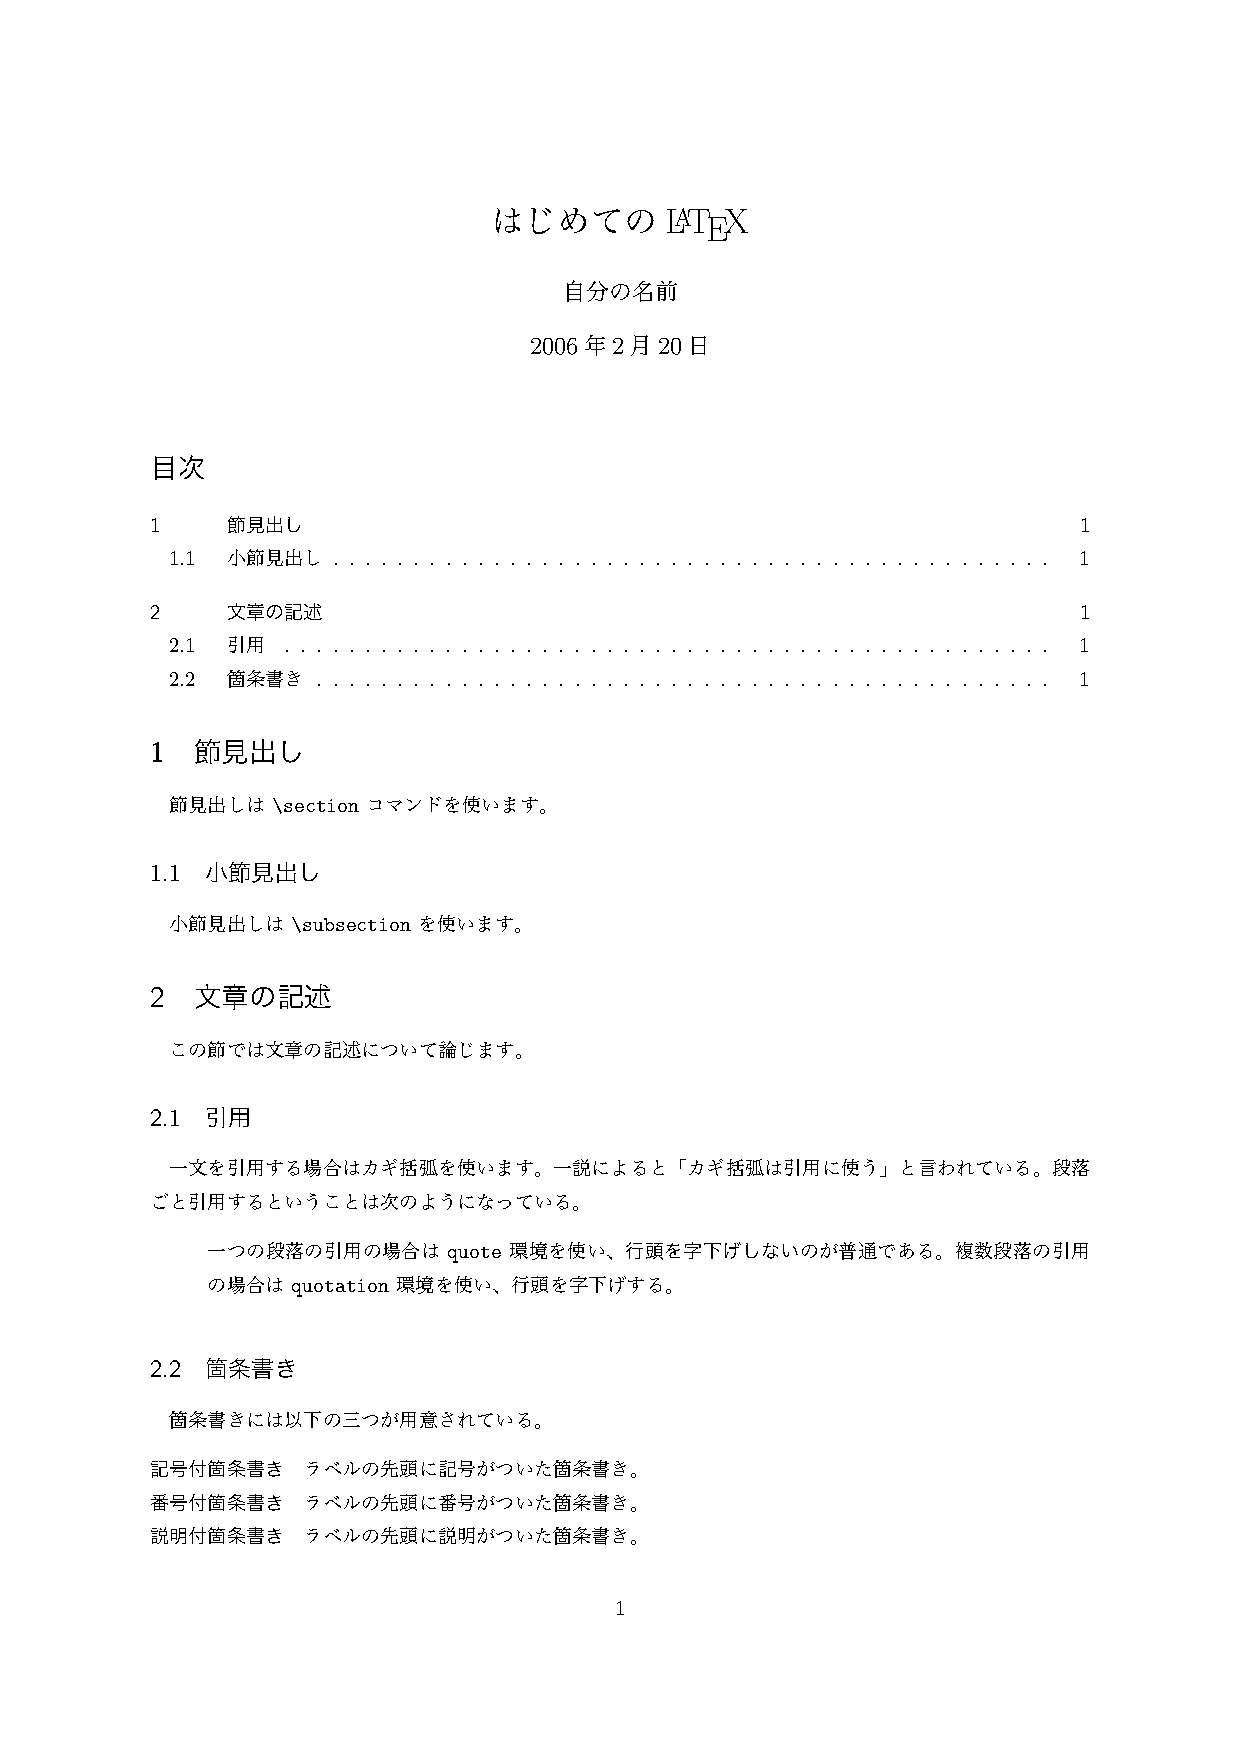
\includegraphics[clip,bb={0 0 595 842},width=\ffullwidth]
   {images/sample}\IOlabel}}
\caption{�ƥ��������Ϥν�����}\label{fig:sample}
\end{figure}

\end{Prob}



\section{���ΤˤĤ���}\seclab{font}

%ʸ���ϰջ���ã���ʤǤ��ä�Ĺ����������
%�������줿���ΤǤ����ܤ�ΰջפ򶯤�
%���᤿���ʤ�пͤϹӡ�����ʸ�����
%�Ǥ��礦����ͥ��������᤿���ʤ��
%�ݤߤ��ӤӤ������ˤʤ�Ǥ��礦����
%��Τ褦��ʸ���η�����Τȸ����ޤ���
%%���ξϤǤ�{\LaTeX}�ǽ��Τ�ɤΤ褦��
%%���äƤ���Τ����������ޤ���
%%ʸ���ϥ��ߥ�˥��������ġ���Ǥ����н�
%%�ʤɤθĿ�Ū��ʸ�Ϥ������ʸ������
%%��˲����������뤿��˻Ȥ�������
%%�������ƻ��Ǥ�������Ū��ʸ���Ȥ�
%%��ƻ���ȤäƤ���䤿���Ǥ�������
%%�ʤϲ��������դˤ����ã��ľ��Ū��
%%���ᡤʸ���Ȥ���ƻ��λȤ��������
%%�Ȥ�������ޤ���
%
%%�ܤäƤ���Ȥ��Ϲӡ�����ʸ����񤯤�
%%���ΤȤ��δ��������䤹���Ǥ��礦��
%%������������Ȥ����Ǥ����ܤäƤ����
%%���˼塹����ʸ����񤤤Ƥ������Ϥ���
%%��ޤ��󡥤���Ϥ��ޤ����Ū�ʻȤ���
%%�Ȥϸ����ޤ���
%
%������ˤϤ�������ΤȤ����ҤȤĤ�
%���Ȥߤ��������Ƥ��ޤ������Τ��ɼԤ�
%�Ф��Ʋ��餫�Υ�å�������ʬ����䤹
%�������뤿����ѹ�������礬�����
%�����Ǥ�������Τ��ѹ�����Ȥ�������
%�ˤ�ɬ����̣������٤��ʤΤǤ������
%�ߤ䤿��˽��Τ��ѹ����Ƥ�դ��ɼԤ�
%���𤵤��ޤ����ޤ���ʬ�����Υ롼���
%���Τ��ѹ����Ƥ��ɼԤˤϲ��ΰ�̣�ʤ�
%����ʬ����ޤ���Τǡ�����Ū�˻Ȥ��
%�Ƥ�����Τ˴ؤ���롼�����Τ��
%�ʡ��Ǥ���
%
%{\LaTeX}��\Z{�ޡ������å�}���Υ����ƥ��
%�Τǥ桼����ľ�ܽ����ѹ��Ѥ�̿
%���Ȥ����Ȥ�����ʤ��ɬ�פΤʤ���
%�Ȥ��Ȼפ��ޤ����ʲ��Υ��ޥ�ɤ�ľ
%�ܻȤ��ΤǤϤʤ������˴Ķ����������
%�Ѥ���Τ�˾�ޤ����Ǥ��礦��

\KY{ʸ��} (\Z{character}) ��\Z{�ջ���ã����}�Ǥ��äơ�
Ĺ�����������������줿\Z{����}�Ǥ����ܤ�ΰջפ򶯤���
�᤿���ʤ�пͤϹӡ�����ʸ����񤯤Ǥ��礦����ͥ������
���᤿���ʤ�дݤߤ��ӤӤ������ˤʤ�Ǥ��礦���ʾ��
�褦��ʸ���η���\KY{����} (\Z{typeface}) �ȸƤӤޤ���

������ǤϤ�������ΤȤ����ҤȤĤ����Ȥߤ��������Ƥ�
�ޤ������Τ��ɼԤ��Ф��Ʋ��餫�Υ�å�������ʬ����䤹
�������뤿����ѹ�������礬����ޤ����Ǥ�������Τ�
�ѹ�����Ȥ������ˤ�ɬ����̣������٤��ʤΤǤ������
�ߤ䤿��˽��Τ��ѹ����Ƥ�դ��ɼԤ��𤵤��ޤ����ޤ�
��ʬ�����Υ롼��ǽ��Τ��ѹ����Ƥ��ɼԤˤϲ��ΰ�̣�ʤ�
����ʬ����ޤ���Τǡ�����Ū�˻Ȥ��Ƥ�����Τ˴ؤ���
�롼�����Τ�ޥʡ��Ǥ���

{\LaTeX}��\Z{�ޡ������å�}���Υ����ƥ�ʤΤǥ桼����
ľ�ܽ����ѹ��Ѥ�̿���Ȥ���������ʤ��ɬ�פΤʤ���
���Ȼפ��ޤ����ʲ��Υ��ޥ�ɤ�ľ�ܻȤ��ΤǤϤʤ���
���˴Ķ�����������Ѥ���Τ�˾�ޤ����Ǥ��礦��


\subsection{ʸ�����礭�����ѹ�}
{\LaTeX}�ˤ����Ƥ����Ū��ñ��ʸ�����礭�����Ѥ���
������ǽ�Ǥ�����ʸ����ʸ�񥯥饹���ץ����ǻ���
��������ʸ�����礭���˱������ѹ�����ޤ� ��ʸ��
���礭�����ѹ��������Ȥ���\tabref{mojinookisa}
��������Υ��ޥ�ɡ�\secref{ml:command}�򻲾ȡˤ�
���Τ褦�˻��Ѥ��ޤ���

\begin{Syntax}
\texttt{\lb}\va{���} \va{ʸ�����礭�����Ѥ�����ʸ����}\texttt{\rb}
\end{Syntax}

\begin{table}[htbp]
\begin{center}
\caption{ʸ�����礭�����ѹ�}\tablab{mojinookisa}
\begin{tabular}{lll}
\TR
\Th{�礭��}       & \Th{̿��}                 & \Th{������}\\
\MR
�ȤƤ⾮���� & \Cmd{tiny}         & {\tiny ��Ļ}\\
���ʤ꾮���� & \Cmd{scriptsize}   & {\scriptsize ��Ļ}\\
������       & \Cmd{footnotesize} & {\footnotesize ��Ļ}\\
��侮����   & \Cmd{small}        & {\small ��Ļ}\\
����         & \Cmd{normalsize}   & {\normalsize ��Ļ}\\
����礭��   & \Cmd{large}        & {\large ����礦}\\
�礭��       & \Cmd{Large}        & {\Large �����礦}\\
���ʤ��礭�� & \Cmd{LARGE}        & {\LARGE �餤���礦}\\
�ȤƤ��礭�� & \Cmd{huge}         & {\huge �Ϥ����礦 }\\
����         & \Cmd{Huge}         & {\Huge �Ҥ��礦}\\
\BR
\end{tabular}
\end{center}
\end{table}
%
\begin{table}[htbp]
\begin{center}
\caption{����ʸ�����礭���ˤ�륳�ޥ�ɤε�ư�ΰ㤤}
\tablab{moji:ookisatte}
 \begin{tabular}{lrrrl}
 \TR
 \Th{���ޥ��}\texttt\bs \Th{�����礭��}& 10\,pt  & 11\,pt   & 12\,pt &
 \Th{���Ѥ��٤�����}${}^{*}$\\
\MR
\Cmd{tiny}        & 5\,pt  & 6\,pt  &  6\,pt & ���겾̾\\
\Cmd{scriptsize}  & 7\,pt  & 8\,pt  &  8\,pt & \\
\Cmd{footnotesize}& 8\,pt  & 9\,pt  & 10\,pt & ������\Z{����}\\
\Cmd{small}       & 9\,pt  & 10\,pt & 11\,pt & ��ɽ���Ф�\\
\Cmd{normalsize}  & 10\,pt & 11\,pt & 12\,pt & �����ḫ�Ф�����ʸ\\
\Cmd{large}       & 12\,pt & 12\,pt & 14\,pt & ���ḫ�Ф�\\
\Cmd{Large}       & 14\,pt & 14\,pt & 17\,pt & �ḫ�Ф�\\
\Cmd{LARGE}       & 17\,pt & 17\,pt & 20\,pt & \\
\Cmd{huge}        & 20\,pt & 20\,pt & 25\,pt & �����ϸ��Ф��ֹ�\\
\Cmd{Huge}        & 25\,pt & 25\,pt & 25\,pt & �����ϸ��Ф�\\
\BR
 \end{tabular}
\\ {\small ${}^{*}$���Ѥ��٤����Ǥ�1���ȤǤξ��Ǥ���}
\end{center}
\end{table}
%
\begin{InOut}
���������С�{\scriptsize ����}�Ͼ�����
ʸ�������ɡ�{\Large ���ä�}���礭��
ʸ���ˤʤäƤ�͡�
\end{InOut}
���Τ褦�ʽ��Τ��礭�����ѹ����륳�ޥ�ɤ�
ľ�ܻȤ��ΤϹ��ޤ����ʤ����������\Z{�ޡ������å�}�դ�
�򤹤�٤��Ǥ����㤨��\Z{��Ĵ}�Τ����ʸ�����礭��
�������ΤǤ���п����� \cmd{kyocho} ̿�����ޤ���
\begin{InOut}
\newcommand\kyocho[1]{{\Large#1}}
\newcommand\Kyocho[1]{{\LARGE#1}}
������\kyocho{����������Ǥ�}�������
\Kyocho{�����Ϥ�ä����}�Ǥ���
\end{InOut}

\subsection{���Τ��ѹ�}\seclab{ouyou:font}
%{\LaTeX}�ˤ����ƽ��Τμ����
%\begin{description}
%\item[\Z{�ե��ߥ꡼}] �ǥ������η����μ��ࡥ
%\item[\Z{���꡼��}]   ����������ʸ�����ΰ㤤�ˤ����ࡥ
%\item[\Z{��������}]   �������Ѳ��ΰ㤤�ˤ����ࡥ
%\item[\Z{������}]     �ե���Ȥ��礭����\zindind{�ե����}{���礭��}%
%\end{description}
%�λͤĤ�ʬ�����ޤ����������˴ؤ��Ƥ����Ҥ��̤�Ǥ���

{\LaTeX}�ˤ����ƽ��Τμ���ϼ��λͤĤ�ʬ�����ޤ���
�������˴ؤ��Ƥ����Ҥ��̤�Ǥ���
\begin{description}
\item[\Z{�ե��ߥ꡼}] �ǥ������η����μ��ࡥ
\item[\Z{���꡼��}]   ����������ʸ�����ΰ㤤�ˤ����ࡥ
\indindz{��}{ʸ����}%
\item[\Z{��������}]   �������Ѳ��ΰ㤤�ˤ����ࡥ
\item[\Z{������}]     �ե���Ȥ��礭����\zindind{�ե����}{���礭��}%
\end{description}

ʸ�����礭������Τμ������ɬ�פ��ѹ�������ϡ�
�դ��ɼԤ��𤵤�������Ǥ�����ʬ�Ϥ�����ȻȤ�ʬ
��������Ǥ��롤�Ȥ�������\tabref{font:family}
�ΰ�������Ŭ�ڤʽ��Τ�����ǡ�������ʸ���������Ƥ�
��������%
\index{�����ޥ���}%
\index{���󥻥����}%
\index{�����ץ饤����}%
\index{�ߥǥ�������}%
\index{�ܡ������}%
\index{��������}%
\index{��������}%
\index{���⡼�륭��ԥ�����}%
\index{�ե��ߥ꡼!�����ץ饤��\zdash}%
\index{�ե��ߥ꡼!���󥻥��\zdash}%
\index{�ե��ߥ꡼!�����ޥ�\zdash}%
\index{��������!���⡼�륭��ԥ���\zdash}%
\index{��������!������\zdash}%
\index{��������!������å�\zdash}%
\index{���꡼��!�ߥǥ�����\zdash}%
\index{���꡼��!�ܡ����\zdash}%
%
% \textnormal, \normalfont ����ĤˤĤ��Ƥ�����
% ���󥳡��ǥ��󥰤ȥե��ߥꡤ���꡼�����������פ�ɸ���
%
\begin{table}[htbp]
\begin{center}
\caption{���Τ��ѹ����륳�ޥ��}\tablab{font:family}
\begin{tabular}{llll}
\TR
\Th{����} & \Th{̿��} & \Th{���} & \Th{����} \\
\MR
�����ޥ�ե��ߥ꡼     & \Cmd{textrm} & \Cmd{rmfamily} &
  \textrm{ABCabc}\\
���󥻥�եե��ߥ꡼   & \Cmd{textsf} & \Cmd{sffamily} &
  \textsf{ABCabc}\\
�����ץ饤���ե��ߥ꡼& \Cmd{texttt} & \Cmd{ttfamily} &
  \texttt{ABCabc}\\
\hline
�ߥǥ����ॷ�꡼��     & \Cmd{textmd} & \Cmd{mdseries} &
  \textmd{ABCabc}\\
�ܡ���ɥ��꡼��       & \Cmd{textbf} & \Cmd{bfseries} &
  \textbf{ABCabc}\\
\hline
��������������     & \Cmd{textit} & \Cmd{itshape} &
  \textit{ABCabc}\\
�����ȥ�������       & \Cmd{textsl} & \Cmd{slshape} &
  \textsl{ABCabc}\\
���⡼�륭��ԥ��륷������ & \Cmd{textsc} & \Cmd{scshape} &
  \textsc{ABCabc}\\
\BR
\end{tabular}
\end{center}
\end{table}

%�ե��ߥ꡼�ȥ��꡼���ȥ������פϤ��줾��
%�Ȥ߹�碌�ƻȤ����Ȥ��Ǥ��ޤ����㤨��
%\yo{����դ��ʤ��������Ʒ������ե����}�Ȥ���ʸ����
%���Ϥ�������м��Τ褦�ˤ��ޤ���
%\begin{InOut}
%\textsf{\textbf{\textit{I like sushi.}}} 
%{\sffamily\bfseries\itshape I like sushi.} 
%\end{InOut}
%���Ѥ��Ƥ�����ܽ��Τˤ�äƤϽ��ϤǤ��ʤ�
%�����פ⤢��ޤ���
%\begin{InOut}
%\texttt{\textbf{Type writer and bold 
% extended?}} I like \textsc{small caps} and
%\textit{\textbf{bold italic}}. {\ttfamily
%\bfseries type writer and bold extended}
%\end{InOut}
%\K{���ΤΥե��ߥ꡼�䥷�����פʤɤ���˻��ꤷ�Ƥ���}
%�礭�����ѹ����ޤ���%������Ū�ˤǤ��ʤ��Τ������Τ��ȤǤ���
%\begin{InOut}
%{\Large\textbf Large Bold?} ������\\
%{\textbf\Large Bold Large?} ���ԡ�
%\end{InOut}
�ե��ߥ꡼�ȥ��꡼���ȥ������פϤ��줾��
�Ȥ߹�碌�ƻȤ������Ǥ��ޤ����㤨��
\yo{����դ��ʤ��������ե����}�Ȥ���ʸ����
���Ϥ�������м��Τ褦�ˤ��ޤ���
\begin{InOut}
\textsf{\textbf{Typeface}}
{\sffamily\bfseries Typeface} 
\end{InOut}
���Ѥ��Ƥ�����ܽ��Τˤ�äƤϽ��ϤǤ��ʤ�
�����פ⤢��ޤ���
\begin{InOut}
\texttt{\textit{Typewriter bold 
extended?}} \textsc{Small Caps}. 
\textit{\textbf{Bold italic}}. 
{\ttfamily \itshape typewriter 
bold extended.}
\end{InOut}
\emph{���ΤΥե��ߥ꡼�䥷�����פʤɤ���˻��ꤷ�Ƥ���
�礭�����ѹ����ޤ�}��
\begin{InOut}
{\Large\textbf Large Bold?} ����\\
{\textbf\Large Bold Large?} ����
\end{InOut}

��ʸ�ν��Τϴ���Ū�ˤ�\Z{��ī��}��
\Z{�����å���}����Ĥ����Ѱդ���Ƥ�
�ޤ���\pp{\tabref{font:wa}}�������
�������ʸ���Ǥ���Ĥν��Τ����Ȥ���
���ä�̾�ĤǤ������ߤ�{\pLaTeX}����ʸ
��¿���Τ�ޤ���Ϥ������񤷤�����
�ޤ��󡥤������Ѱդ���ʸ��¿���Τˤ���
���ɼԤ�����˴���Ƥ��ʤ��Ȼפ��ޤ�
�Τǡ��̤˹Ԥ�ʤ��ۤ����ɤ����⤷��ޤ���
\begin{table}[htbp]
\begin{center}
\caption{��ʸ���ΤΥե��ߥ꡼}\tablab{font:wa}
  \begin{tabular}{llll}
\TR
 \Th{����} & \Th{̿��} & \Th{���} & \Th{����}\\
\MR
% ��ī�ե��ߥ꡼& \Cmd{textmc} & 
%   \Cmd{mcfamily} & \textmc{�ʻ�Ȭˡ�äƲ��Ǥ�����}\\
% �����å��ե��ߥ꡼&\Cmd{textgt} & 
%   \Cmd{gtfamily} & \textgt{�ʻ�Ȭˡ�äƲ��Ǥ�����}\\
 ��ī�ե��ߥ꡼& \Cmd{textmc} & 
   \Cmd{mcfamily} & \textmc{�ʻ�Ȭˡ�Ȥϲ��Ǥ�����}\\
 �����å��ե��ߥ꡼&\Cmd{textgt} & 
   \Cmd{gtfamily} & \textgt{�ʻ�Ȭˡ�Ȥϲ��Ǥ�����}\\
\BR
 \end{tabular}
\end{center}
\end{table}
\indindz{��Ĵ}{���Ф���}\indindz{��Ĵ}{��ʸ��}%%
\begin{InOut}
��ʸ���Ǥˤ�������ī�Τ��̾��ʸ�Ϥ���
�ǡ������å��Τ�\textgt{ʸ�Ϥζ�Ĵ��}
�Ȥ��ޤ���{\gtfamily ���Ф��⶯Ĵ��
�٤����ǤʤΤǥ����å��Τˤ���Τ�����
�Ǥ�}��
\end{InOut}


\subsection{���ܽ��Τ��ѹ�}
�ե���Ȥ��礭����ե��ߥ꡼�ʤɤ���ꤹ��̿���
ʬ����ޤ�������������ʸ��˻Ȥ��Ƥ������
���Τ�Τ��ѹ�����ˤϤɤ�������ɤ��ΤǤ��礦����
�¤����ʲ����ʤ�{\LaTeX}��ʸ������򤷤Ƥ���Ȥ���
�Ȥ��Ƥ��벤ʸ�Υե���Ȥ�\Person{Donald}{Knuth}��
�ǥ����󤷤�\Z{Computer Modern}�ȸƤФ��
\KY{���ܽ���}�ˤʤäƤ��ޤ������δ��ܽ��Τ���
��Τ��ѹ�����ˤϴ��ܽ��Τ��ѹ�����������ʤ��줿��
�������ɤ߹��फ����ʬ�ǻ��ꤹ��ɬ�פ�����ޤ���
�����˻Ȥ���������Τˤ����Ū��{Computer Modern}
���Ȥ��ޤ����ե���ȤˤĤ��Ƥ�
\Hito{��¼}{��ɧ}��ʸ��~\cite{bibunsyo3}�ʤɤ򻲾Ȥ��Ƥ�
���������ܽ�Ǥϼ�갷���ޤ���
�����Ƹ����ʤ��%
\Person{Young}{Ryu}����������\Sty{txfonts}��Ȥ��Τ�
��ڤǤϤʤ����Ȼפ��ޤ���ɸ�����ۤ�Times�Ϥ�
�ե���Ȥ�Ȥ��褦�ˤ���\Sty{mathptmx}�䡤Palatino��
�Υե���Ȥ�Ȥ��褦�ˤ���\Sty{mathpazo}����
\Sty{pxfonts}��\Sty{txfonts}�Ȥ��������⤢��ޤ���\secref{app:typeface}
�򻲾ȡˡ�


\section{ʸ�Ϥν���}
\zindind{����}{���}%
%���Τ褦�ˤ��ƴ���Ū��ʸ�Ϲ�¤���Ȥ߾夲�ơ����Ū�˻�ξ�ʤɤ�
%���Ϥ���櫓�Ǥ�������ȯ�Ǵ�����ʸ��ˤʤ뤳�ȤϤۤȤ�ɤ���ޤ���
%���٤⽤���Ȳ�ɮ�򷫤��֤����ǽ�Ū����ʸ�˻ž夬���ΤȻפ��ޤ���
%
%���ΤȤ���ɬ�פʤΤ�ʸ�Ϥι����˴ؤ����«���Ǥ���
%{\LaTeX}�ǤϤۤȤ�ɤ�¿���ν�����Ⱦ��ưŪ�˹Ԥ��Τǡ�
%���ʤϵ��ˤʤ�ʤ���ʬ�Ǥ����㤨��Ⱦ�ѱѿ��������Ѥ�
%���ܸ�ȤΤ������ˤϻ�ʬ�����Ȥ��äơ����Ѷ����4ʬ��1��
%���ڡ��������������ꡤ�Ԥ���Ƭ�˶����������äƤϤ����ʤ�
%�Ȥ�������Ƭ��§�����������{\LaTeX}\pp{{\pTeX}�ˤ�����}��
%Ⱦ��ư�ǹԤ��ޤ���
%
%���Τ褦�ʼ�ưŪ�ʽ����ʳ��ˤ�桼��¦�����ϥߥ��ˤ�꽤��
%��ɬ�פˤʤ��礬����ޤ������ξ���1�ٺ�������ʸ�Ϥ���
%����~\cite{kumihan3}�ʤɤ�Ȥäƽ�������Τ��ɤ��Ǥ��礦��
%
%���ߤǤ�ʸ�Ϥϥ���ԥ塼����Ǥ��٤��Ȥळ�Ȥ��Ǥ���Τǡ�
%�ְ㤤�򸫤Ĥ����餽�ξ�Ǥ����˽�����ǽ�Ǥ��� ��˰�����
%�ƥ����å�����Ȥ�����Ȥ����ΨŪ���⤷��ޤ��󡥥����
%�塼���Υ�˥�����Ȱ�����������ξ�Ԥ�������褫����ʸ��
%�������Ƥ���������
%ʸ�Ϻ���������դ��٤����Ȥ���
%\begin{itemize}
% \item 1ʸ��Ĺ���������Ƥ��ʤ�����
% \item �Ǥ���Ĵ�����줵��Ƥ��뤫��
% \item ������δط���Ϥä��ꤷ�Ƥ��뤫��
% \item Ʊ���۵���ʤɤδְ㤤�Ϥʤ�����
% \item ����ζ��ڤꡤ�Ϥζ��ڤ�����Τ���
%\end{itemize}
%�ʤɤ��󤲤��ޤ���

���Τ褦�ˤ��ƴ���Ū��ʸ�Ϥ�������¤���Ȥ߾夲�ơ����Ū�˻�
�ξ�ʤɤ˽��Ϥ���櫓�Ǥ�������ȯ�Ǵ�����ʸ��ˤʤ���Ϥ�
�Ȥ�ɤ���ޤ��󡥲��٤⽤���Ȳ�ɮ�򷫤��֤����ǽ�Ū����ʸ��
�ž夬���ΤȻפ��ޤ���

���ΤȤ���ɬ�פʤΤ�ʸ�Ϥι����˴ؤ����«���Ǥ���{\LaTeX}��
�ϤۤȤ�ɤ�¿���ν�����Ⱦ��ưŪ�˹Ԥ��Τǡ����ʤϵ��ˤʤ��
����ʬ�Ǥ����㤨��Ⱦ�Ѥαѿ��������Ѥ����ܸ�ȤΤ������ˤ�
\Z{��ʬ����}�Ȥ��äơ����Ѷ����4ʬ��1�Υ��ڡ��������������ꡤ
�Ԥ���Ƭ�˶����������äƤϤ����ʤ��Ȥ�������Ƭ\Z{��§����}��
�����{\LaTeX}\pp{{\pTeX}�ˤ�����}��Ⱦ��ư�ǹԤ��ޤ���
% �н褹��Ȥ���ɽ��������Ŭ�ڤǤϤʤ�����������

\indindz{����}{����}%
\index{�ְ㤤�ν���}%
���Τ褦�ʼ�ưŪ�ʽ����ʳ��ˤ�桼��¦�����ϥߥ��ˤ�꽤��
��ɬ�פˤʤ��礬����ޤ������ξ���1�ٺ�������ʸ�Ϥ�\Z{����}
����~\cite{NES1999}�ʤɤ�Ȥäƽ�������Τ��ɤ��Ǥ��礦��


���ߤǤ�ʸ�Ϥϥ���ԥ塼����Ǥ��٤��Ȥ�����Ǥ���Τǡ�
�ְ㤤�򸫤Ĥ����餽�ξ�Ǥ����˽�����ǽ�Ǥ��� ��˰�����
�ƥ����å�����Ȥ�����Ȥ����ΨŪ���⤷��ޤ��󡥥����
�塼���Υ�˥�����Ȱ�����������ξ�Ԥ�������褫����ʸ��
�������Ƥ���������
ʸ�Ϻ���~\cite{HO2004,HO2002,KK1981}������դ��٤����Ȥ���
�ʲ��ι��ܤʤɤ��󤲤��ޤ���
\begin{itemize}
 \item 1ʸ��Ĺ���������Ƥ��ʤ�����
 \item �Ǥ���Ĵ�����줵��Ƥ��뤫��
 \item ������δط���Ϥä��ꤷ�Ƥ��뤫��
 \item Ʊ���۵���ʤɤδְ㤤�Ϥʤ�����
 \item ����ζ��ڤꡤ�Ϥζ��ڤ�����Τ���
\end{itemize}


%\subsection{���ڥ�����å�}
%��ʸ��ʸ��ξ��ϥ��ڥ�ߥ�������å��Ǥ���ץ�����ब
%�����Ĥ�����ޤ���

\subsection{��ʸ�����å�\zdash\Y{syntonly}}
{\LaTeX}�θ��Ƥ�񤤤Ƥ���ȡ����ޥ�ɹ�ʸ�ε��ҥߥ��򤷤�
���ޤ���������ޤ�����̤�­��ʤ��Ȥ�����ʸ���Ⱦ�ʸ����񤭴ְ㤨�Ƥ���
�ʤɤǤ���
\Person{Frank}{Mittelbach}��\Person{Rainer}{Sch\"opf}����������
\Sty{syntonly}��Ȥ��ȡ���ʬ�ε��Ҥ��ְ�äƤ��ʤ������ºݤν��Ϥ򤻤���
��ʸ�Υ����å�������Ԥ��褦�ˤǤ��ޤ���
%
\Cmd{syntaxonly}̿���ץꥢ��֥�˵��Ҥ��ޤ���\Sty{syntonly}�ѥå�����
���ɤ߹���������Ǥϲ��ⵯ����ޤ���
%
��ʸ����������å�����Τ��̾��DVI���Ϥ�ȼ�������ץ��åȤ��������®
���Ȼפ��ޤ���

\begin{InTeX}
\documentclass{jarticle}
\usepackage{syntonly}
\syntaxonly
\begin{document}
I like {\LaTex}.%����ϥ��顼�ˤʤ�ޤ���
\end{document}
\end{InTeX}


\section{���饹�ȥѥå�����}\seclab{class}
{\LaTeX}��\Z{�ޡ������å�}��������Ѥ�������ʤΤ�\Z{��}�����Ƥ�
ʬΥ�����Τ�����Ū�Ǥ���������\Z{���饹}\pp{\Z{class}}��
\Z{�ѥå�����}\pp{\Z{package}}�Ȥ�����ĤΥե������Ȥ�
�褦�ˤʤäƤ��ޤ���

%���ơ����饹��ѥå������Ȥ����Ѹ줬�ФƤ��ޤ���������ñ
%���������ޤ��礦���Τ��ä��֤��Ȥ���\pp{{\LaTeX2.09}}��
{\LaTeX}�Ǥ�ʸ��ν񼰤���ꤹ�뤿��˥��饹�Ȥ������
��������ޤ������饹��\Z{�ɥ�����ȥ��饹}�Ȥ�
\Z{ʸ�񥯥饹}�ʤɤȸƤФ�Ƥ��ޤ����ޤ��������ʵ�ǽ%
\zindind{�ޥ���}{�ѥå�����}%
�򽸤᤿��Τ�\K{�ѥå�����}�ȸƤӤޤ����ѥå�������\K{�ޥ����ѥå�����}
�Ȥ�������ñ��\KY{�ޥ���}�ʤɤȸƤФ�ޤ���

�������ơ�{\LaTeX}�θ���\pp{\Z{�������ե�����}}�Ǥ�ɬ��ʸ
�����Ƭ��
\begin{Syntax}
\cmd{documentclass}\opa{���ץ����$,\ldots$}\pa{���饹}\\ 
\cmd{usepackage}\opa{���ץ����$,\ldots$}\pa{�ѥå�����}
%\cmd{documentclass}\opa{���ץ����}\pa{���饹}\\ 
%\cmd{usepackage}\opa{���ץ����}\pa{�ѥå�����}
\end{Syntax}
�Τ褦�ʵ��Ҥ򤷤ơ�ʸ��ν񼰤��绨�Ĥ˷��ꤷ�ޤ���

%�㤨�С����ܸ�ξ����Ϥβ�����ޤߡ����Τ��礭����11�ݥ���Ȥ�
%\Z{2����}�ε�����񤳤��Ȼפ���
�㤨�С���ʸ�����ܸ�Dz�����ޤߡ����Τ��礭����11�ݥ���Ȥ�
\Z{2����}�ε�����񤳤��Ȼפ��м��Τ褦�˸������������ޤ���

\begin{InTeX}
\documentclass[twocolumn,11pt]{jarticle}
\usepackage[dvips]{color}
\usepackage[dvips]{graphicx}
\end{InTeX}

���Ѥ��륯�饹����ˤϥ��ץ����
¸�ߤ����嵭�Τ褦��2���ȤΤ����\option{twocolumn}��ե���Ȥ�
�礭������ꤹ�뤿���\option{11pt}�Ȥ������ץ�������ꤷ�ޤ���
�ޤ����ͤε����ʤ��¤ꡤʣ���Υѥå�������Ȥ�����
Ʊ��������������Ǥ��ޤ���

\begin{InTeX}
\documentclass[twocolumn,11pt]{jarticle}
\usepackage[dvips]{graphicx,color}
\end{InTeX}

���饹�ȥѥå����������Τ˶��̤��뤿���
���饹��\Z{��ĥ��}�ˤ�\exten{cls}��
�ѥå������γ�ĥ�Ҥˤ�\exten{sty}���դ���褦�ˤ��ޤ���

\subsection{ɸ��Ū�ʥ��饹}\seclab{01pregame:sec:classes}

\indindz{���饹}{ɸ��Ū��}%
{\LaTeX}��{\pLaTeX}���ϰ�����󶡤���Ƥ���ɸ��Ū�ʥ��饹��
�Ҳ𤷤ޤ������饹�ե������\Va{classes}{dtx}��
\Va{classes}{ins}�Ȥ�����ĤΥե���������ۤ�������¿��
�褦�Ǥ���

���륯�饹�������饤�󥹥ȡ���Ǥ���Τ��ϡ����ǤˤǤ�
�夬�äƤ��륯�饹�ե�����\Va{classes}{cls}��¸�ߤ����
���Υե��������Ƭ��ʬ�˼��Τ褦�ʵ��Ҥ�����ޤ���

\begin{InTeX}
%% This is file `class.cls',
%% generated with the docstrip utility.
%% The original source files were:
%% classes.dtx  (with options: `option')
\end{InTeX}

���ꥸ�ʥ�Υ������ե������
���ץ�����\option{`option'}����ꤷ�ƥե�����̾��
\Va{classes}{dtx}�Ǥ������������Ƥ���Ƥ��ޤ��Τ�
Unix��OS�ʤ��
\begin{InTerm}
  \type{find /usr/local/share/texmf/ -name classes.dtx}
\end{InTerm}
�ʤɤǤ��Υե�����򸡺��Ǥ���Ǥ��礦��Windows��Macintosh
�ϥե�����θ����ε�ǽ������Ȼפ��ޤ��Τǡ��������Ȥ���
�ɤ��Ǥ��礦�����Τ褦�ˤ��Ƹ�����������\Va{classes}{dtx}��
\Va{classes}{ins}��¸�ߤ��ޤ������Υե����뤬������˰�ư����
%\begin{InTerm}
  \type{platex classes.dtx}
%\end{InTerm}
�Ȥ���Ф��Υ��饹�λ��ͽ�򸫤�����Ǥ��ޤ��������
%\begin{InTerm}
  \type{platex classes.ins}
%\end{InTerm}
�Ȥ���Ȥ��Υ��饹��Ƴ����������Ǥ��ޤ������Τ褦�����򤹤��
\Sty{DocStrip}�Ȥ����ޥ�����Ŭ�ڤ˥ե������������ޤ���
�㤨�Хե�����\Fl{classes.ins}�򤳤Τ褦�˽�������ȡ�
\Fl{article.cls}��\Fl{report.cls}��\Fl{book.cls}��\Fl{bk10.clo}��
\Fl{bk11.clo}��\Fl{bk12.clo}��\Fl{size10.clo}��\Fl{size11.clo}��
\Fl{size12.clo}�Ȥ�����ĤΥե����뤬��������ޤ���

���ܸ��ޤޤʤ��褦��ʸ��ˤϲ�ʸ���ѤΥ��饹�����ѤǤ��ޤ���
���줾��ɤΤ褦��ʸ���������������ˤ�äƲ����Ѥ��뤫��
ʬ����ޤ���ɸ��Ǥϰʲ��β�ʸ�ѤΥ��饹���Ȥ��ޤ���
\begin{namelist}{xxxx}
\item[\Cls{article}] �����Ϥε�����������뤿��Υ��饹��
	\Fl{classes.dtx}��{\COMP}�˾ܤ������ͤ��񤫤�Ƥ��롥
\item[\Cls{report}]  �����������뤿��Υ��饹��
	Ʊ����\Fl{classes.dtx}��{\COMP}�˾ܤ������ͤ��񤫤�Ƥ��롥
\item[\Cls{book}]    ���Ҥ�������뤿��Υ��饹��
	Ʊ����\Fl{classes.dtx}��{\COMP}�˾ܤ������ͤ��񤫤�Ƥ��롥
\item[\Cls{slides}]  ���饤�ɤ�������뤿��Υ��饹��
	\Fl{slides.dtx}�˾ܤ������ͤ��񤫤�Ƥ��롥
\item[\Cls{proc}]    \cls{article}��١����˵Ļ�Ͽ�ʤɤ�%
	�������뤿��Υ��饹��
	\Fl{proc.dtx}�˾ܤ������ͤ��񤫤�Ƥ��롥
%\item[\cls{ltxdoc}��\cls{ltxguide}��\cls{ltnews}] 
%	��ȯ���ѤΥ��饹�ե����롥���̥桼���ˤϤ��ޤ��Τʤ���Ρ�
%	���줾�졤\fl{ltxdoc.dtx}��\fl{ltxguide.dtx}��
%	\fl{ltnews.dtx}�˾ܤ������ͤ��񤫤�Ƥ��롥
%\item[\cls{minimal}] {\LaTeX}���갷����ǺǾ��¤������
%�������饹�ե����롥���Υ��饹�򸵤˼�ʬή�Υ��饹�򿷤���
%��ȯ���뤳�Ȥ�Ǥ��롥
\end{namelist}
�ʾ��\cls{article}��\cls{report}��\cls{book}�λ��Ĥ�ޤȤ��
\Cls{classes}�ȸƤֻ�������ޤ���

���ܸ��ʸ��Ǥϡ�ɸ��ǰʲ��Υ��饹���Ȥ��ޤ���
\begin{namelist}{xxxxx}
\indindz{���饹}{�����Ϥ�ʸ���Ѥ�}
\item[\Cls{jarticle}] �����Ϥ����ܸ�ε�����������뤿��Υ��饹��
\indindz{���饹}{�����Ѥ�}
\item[\Cls{jreport}]  ���ܸ�������������뤿��Υ��饹��
\indindz{���饹}{�����Ѥ�}
\item[\Cls{jbook}]    ���ܸ�ν��Ҥ�������뤿��Υ��饹��
\item[\Cls{tarticle}] �Ľ񤭤ξ����Ϥ����ܸ�ε�����������뤿��Υ��饹��
\item[\Cls{treport}]  �Ľ񤭤����ܸ�������������뤿��Υ��饹��
\item[\Cls{tbook}]    �Ľ񤭤����ܸ�ν��Ҥ�������뤿��Υ��饹��
\end{namelist}
�ʾ��\cls{jarticle}��\cls{jreport}��\cls{jbook}�λ��Ĥ�ޤȤ��
\Cls{jclasses}�ȸƤֻ�������ޤ���

\subsection{���饹���ץ����}\seclab{classopt}
�ɥ�����ȥ��饹\pp{ʸ�񥯥饹}�ˤϤ⤦�����ܺ٤�
�����Ԥ������Ǥ��ޤ���\cmd{documentclass}��Ǥ�հ����Ȥ���
���Ҥ��ޤ���¿���Υ��饹�ե�����Ǥϼ���\Z{���饹���ץ����}��
�Ȥ���Ȼפ��ޤ���
%\begin{description}
%
%\item[\Z{ʸ��������}\av{\Optionlist{10pt,11pt,12pt}}]
%���ƤǴ��ܤȤʤ�ʸ�����礭������ޤ�������ʸ����������
%���Ȥ��Ƥ��ޤ��ޤʥѥ�᡼�������ꤵ��ޤ���ɸ���
%\option{10pt}��
%
%\item[\Z{�ѻ極����}\av{\Optionlist{a4paper,a5paper,b5paper,letterpaper}}]
%���Ƥ��ѻ���礭������ꤷ�ޤ���\index{�ѻ�!\zdash �Υ�����}%
%\index{�ѻ�!\zdash ���礭��}%
%��ʸ�ξ��Ϥ���¾��\Optionlist{b4paper,a4j,a5j,b4j,b5j}�ʤɤǤ���
%\sty{geometry}�ѥå�������\cls{jsclasses}��Ȥ������������
%������ޤ���
%
%\item[\Z{�ѻ�����}\av{\Option{landscape}}]
%�ѻ���֤��ˤ��ޤ���ɸ��Ͻ��֤��Ǥ���\index{�ѻ�!\zdash ������}
%
%\item[\Z{������}\av{\Optionlist{oneside,twoside}}]
%�ѻ������\pp{\option{oneside}}�����˰������뤫
%����Ȥ�ξ��\pp{\option{twoside}}�˰������뤫����ꤷ�ޤ���
%\item[\Z{����}\av{\Optionlist{onecolumn,twocolumn}}]
%%\ex{����}{1����}\index{����}{2����}%
%\Z{1����}\pp{\option{onecolumn}}�ˤ��뤫\Z{2����}\pp{\option{twocolumn}}
%�ˤ��뤫����ꤷ�ޤ���
%
%\indindz{ɽ��}{��Ω�ڡ�����}\indindz{ɽ��}{Ʊ�ڡ�����}\indindz{�ڡ���}{ɽ��}
%\item[\Z{ɽ��}\av{\Optionlist{titlepage,notitlepage}}]
%ɽ�����Ω���ƽ��Ϥ���\pp{\option{titlepage}}����
%Ʊ���ڡ����˽��Ϥ���\pp{\option{notitlepage}}���Ȥ���ɽ���
%�쥤�����Ȥ���ꤷ�ޤ���
%
%\item[{�������}\av{\Option{fleqn}}]
%\zindind{����}{���}%	   
%�̹Կ����ΰ��֤�·���˻��ꤷ�ޤ���ɸ������·���Ǥ���
%	
%\item[{�����ֹ�ΰ���}\av{\Option{leqno}}]
%\zindind{����}{�ֹ�ΰ���}%
%�����ֹ�ΰ��֤�¦�˻��ꤷ�ޤ���ɸ��ϱ�¦�Ǥ���
%	
%\item[\Z{�ɥ�ե�}\av{\Optionlist{draft,final}}]
%ʸ����ΰ��Ϥ߽Ф��Ƥ��ޤä��ս�˰���Ĥ��뤫�ɤ�����
%��ɮ����ǰ�������Ȥ��ˤϥɥ�եȥ⡼�ɤˤ��롥
%�ɥ�եȥ⡼�ɤ�\option{draft}��
%���Ƥ�����������\option{final}���ѹ����롥
%ɸ���\option{final}��
%
%\item[\Z{��������}\av{\Optionlist{openright,openany}}]
%\cls{(j)report}��\cls{(j)book}�ˤ����ƾϤʤɤγ��ϥڡ�����
%����򤹤롥��˴���ڡ����ǵ�����\pp{\option{openright}}����
%�ɤ��餫��Ǥⵯ����\pp{\option{openany}}�������ꤹ�롥
%\cls{(j)report}��ɸ���\option{openany}��
%\cls{(j)book}��ɸ���\option{openright}��
%\end{description}

\begin{description}
\item[{ʸ��������}\av{\Optionlist{10pt,11pt,12pt}}] 
\zindind{ʸ��}{������}%
\zindind{����}{��ʸ��������}%
���ƤǴ��ܤȤʤ�ʸ�����礭������ޤ�������ʸ����������
���Ȥ��Ƥ��ޤ��ޤʥѥ�᡼�������ꤵ��ޤ���ɸ���
\option{10pt}��

\item[{�ѻ極����}\av{\Optionlist{a4paper,a5paper,b5paper,letterpaper}}]
���Ƥ��ѻ���礭������ꤷ�ޤ���
\index{�ѻ�!\zdash �Υ�����}%
\index{�ѻ�!\zdash ���礭��}%
\zindind{����}{���ѻ極����}%
��ʸ�ξ��Ϥ���¾��\Optionlist{b4paper,a4j,a5j,b4j,b5j}�ʤɤǤ���
\sty{geometry}�ѥå�������\cls{jsclasses}��Ȥ������������
������ޤ���

\item[{�ѻ�����}\av{\Option{landscape}}]
�ѻ���֤��ˤ��ޤ���ɸ��Ͻ��֤��Ǥ���\index{�ѻ�!\zdash ������}

\item[\Z{������}\av{\Optionlist{oneside,twoside}}]
�ѻ������\pp{\option{oneside}}�����˰������뤫
����Ȥ�ξ��\pp{\option{twoside}}�˰������뤫����ꤷ�ޤ���
\item[\Z{����}\av{\Optionlist{onecolumn,twocolumn}}]
\indindz{����}{1}\indindz{����}{2}%
\Z{1����}\pp{\option{onecolumn}}�ˤ��뤫\Z{2����}\pp{\option{twocolumn}}
�ˤ��뤫����ꤷ�ޤ���

\indindz{ɽ��}{��Ω�ڡ�����}\indindz{ɽ��}{Ʊ�ڡ�����}\indindz{�ڡ���}{ɽ��}
\item[{ɽ��}\av{\Optionlist{titlepage,notitlepage}}]
ɽ�����Ω���ƽ��Ϥ���\pp{\option{titlepage}}����
Ʊ���ڡ����˽��Ϥ���\pp{\option{notitlepage}}���Ȥ���ɽ���
�쥤�����Ȥ���ꤷ�ޤ���

\item[{�������}\av{\Option{fleqn}}]
\zindind{����}{���}%	   
�̹Կ����ΰ��֤�·���˻��ꤷ�ޤ���ɸ������·���Ǥ���
	
\item[{�����ֹ�ΰ���}\av{\Option{leqno}}]
\zindind{����}{�ֹ�ΰ���}%
�����ֹ�ΰ��֤�¦�˻��ꤷ�ޤ���ɸ��ϱ�¦�Ǥ���
	
\item[\Z{�ɥ�ե�}\av{\Optionlist{draft,final}}]
\indindz{����}{�ɥ�ե��ʳ���}%
\indindz{����}{��ɮ�ʳ���}%
��ɮ����ǰ�������Ȥ���\option{draft}���ץ������դ���ȡ�
ʸ�������ΰ��Ϥ߽Ф��Ƥ��ޤä��ս�˰����դ��Ƥ���ޤ���
���Ƥ�����������\option{final}���ѹ����ޤ���ɸ���\option{final}�Ǥ���

\item[\Z{��������}\av{\Optionlist{openright,openany}}]
\cls{(j)report}��\cls{(j)book}�ˤ����ƾϤʤɤγ��ϥڡ�����
����򤷤ޤ�����˴���ڡ����ǵ�����\pp{\option{openright}}����
�ɤ��餫��Ǥⵯ����\pp{\option{openany}}�������ꤷ�ޤ���
\cls{(j)report}��ɸ���\option{openany}��
\cls{(j)book}��ɸ���\option{openright}��
\end{description}


�Ƕ�Ǥϡ�\Hito{��¼}{��ɧ}���������Ƥ���
\Cls{jsclasses}�Ȥ������饹�ե����뷲����ɾ������ޤ�\footnote{\webJsclasses}��
���Υ��饹����Ƴ�������
\begin{namelist}{xxxxxx}
\item[\Cls{jsarticle}]	�����Ϥ����ܸ�ε�����������뤿��Υ��饹��
\item[\Cls{jsbook}]	���ܸ�ν��Ҥ������������뤿��Υ��饹��
\item[\Cls{jspf}]	˿�ز���ѤΥ��饹��
\end{namelist}
�λ��Ĥ����ѤǤ��ޤ��������Υ��饹�ǻ���Ǥ���
���饹���ץ����\cls{jclasses}���ɲä����
���ޤ�\footnote{\cls{(j)classes}���������Ƥ��������Ĥ���
���饹���ץ���󤬼�������Ƥ��ޤ���}��
�ʾ��\cls{jsarticle}��\cls{jsbook}��\cls{jspf}�λ��Ĥ�ޤȤ��
\Cls{jsclasses}�ȸƤӤޤ���

\begin{description}
\item[\Z{ʸ��������}]\av{\Optionlist%
   {9pt,10pt,11pt,12pt,14pt,17pt,20pt,21pt,25pt,30pt,36pt,43pt,12Q,14Q}}
\item[\Z{�ѻ極����}]\av{\Optionlist%
   {a4paper,a5paper,a6paper,b5paper,b4paper,a4j,a5j,b4j,b5j,a4var,b5var}}
\item[������]\av{\Option{english}}
  ��ʸ�Ѥθ��Ф�������ȹ�����ˤʤ�ޤ���
\item[�ѻ極��������] \av{\Option{papersize}} 
  �ѻ極�����ξ����ǥХ����ɥ饤�Ф��Ϥ��褦�ˤ��ޤ���
\item[��ݡ��Ⱥ���] \av{\Option{report}} 
  \Z{��ݡ��Ⱥ���}�Ѥ� \cmd{chapter} ̿���Ȥ������Ǥ��ޤ���
  \cls{jsbook} �ǤϺ����������˴ؤ������꤬�Ѥ��ޤ���
\end{description}

\subsection{ɸ��ǻ��ѤǤ���ѥå�����}\seclab{01pregame:sec:stdmacro}
{\LaTeX}��Ƴ������Ȱ���ź�դ����ɸ��Ū�ʥѥå�����������ޤ���
�����ϥץꥢ��֥���ʬ�˼��Τ褦�ˤ���Ȼ��Ѳ�ǽ�ˤʤ�ޤ���
\begin{Syntax}
\C{usepackage}\opa{���ץ����}\pa{�ѥå�����}
\end{Syntax}

�ƥѥå������ξܺ٤��������ɤߤ����Ȥ���
\begin{InTerm}
   \type{platex filename.dtx}
\end{InTerm}
�Ȥ����\Va{filename}{dvi}����������ޤ�\footnote{�Ƕ��\TeX �Ķ�
�Ǥ� \underline{\str{texdoc }\va{�ѥå�����̾}}���Ȥ���Хޥ˥奢��
��ɽ������ޤ���}�������κ�����
�ܼ��κ�������߻��Ȥβ��ʤɤ򤹤�д�����DVI�ե����뤬
�������ޤ����ƥ������ե�����ؤθ����ѥ����ʤ����
��������\Va{filename}{dtx}�򸡺�������ϤǤ��ޤ���
{Windows}�ʤ�Хե�����θ�����Unix��OS�ʤ��\prog{find}���ޥ��
�ʤɤ�õ���Ƥ��������������{\LaTeX}�򥤥󥹥ȡ��뤷��
�ǥ��쥯�ȥ�\pp{�ե����}�β�\qu{\fl{\$texmf/tex/latex/base}}�ˤ���ޤ���
%\begin{namelist}{xxxxxx}
%\item[\Sty{alltt}]	\Env{alltt}�Ķ����󶡤��뤿��Υޥ�����
%���δĶ���Ǥ�\verb|\|��\verb|{|��\verb|}|���̾��̤��̿��Ȥ���
%��ᤵ�졤{\LaTeX}�Υ��ޥ�ɤʤɤ��Ȥ��롥\Fl{alltt.dtx}����
%��������롥
%\item[\Sty{doc}]	�ѥå������ե����뤬ɬ�פȤ���ޥ�����
%\Fl{doc.dtx}������������롥
%\item[\Sty{exscale}]	\Fl{exscale.dtx}
%\item[\Sty{fontenc}]	\Fl{fontenc.dtx}
%\item[\Sty{graphpap}]	\Fl{graphpap.dtx}
%\item[\Sty{ifthen}]	\Fl{ifhten.dtx}
%\item[\Sty{inputenc}]	\Fl{inputenc}
%\item[\Sty{latexsym}]	\Fl{latexsym}
%\item[\Sty{makeidx}]	���������ѤΥޥ�����
%\Fl{makeindx.dtx}������������롥
%\item[\Sty{newlfont}]	\Fl{newlfont.dtx}
%\item[\Sty{oldlfont}]	\Fl{oldlfont.dtx}
%\item[\Sty{syntonly}]	�ºݤν��Ϥ򤻤��ˡ���ʸ���ϤΤߤ�Ԥ��ޥ�����
%\Fl{syntonly.dtx}������������롥
%\item[\Sty{tracefnt}]	ʸ����ǻ��Ѥ������Τξ����ܤ���
%ɽ�����뤿��Υޥ�����\Fl{ltfsstrc.dtx}������������롥
%\end{namelist}
%�����Υե�����ˤĤ��ƾܤ�����\wasyo{\LMANUAL}��
%\wasyo{\COMP}�򸫤Ƥ����������������Ǥ����ޤ�����������Ǥ�
%�����䤷���Τǡ�����ͭ�פ�{\LaTeX}��
%�ؤ��륦���֥ڡ������ʤ���õ�����Ȥˤʤ�櫓�Ǥ�����
%\wasyo{\LMANUAL}��
%Ķ�����Τ�¸�ߤ��ʤ��Τ������Ǥ���\yo{��Ԥ��ܤ�����ʬ����䤹��
%ʸ�񤬥����֥ڡ�����¸�ߤ�����ޯ��ˤʤ��嵐��}�Ȥ������դ���
%�ޤ��ɤ�����Ȥ�ʤ�ʹ�����Ƥ����ΤǤ����դ������򽪤��ޤ���

{\LaTeX}������ԥ塼����Ƴ������Ƥ���ʤ�аʲ��α���Ū��
�ޥ����䥽�եȥ�������Ʊ������Ƥ�����Ǥ��礦��
�����Υե�����ϲ�ʸ��ʸ���������뤦���Ǥ�ɬ�ܤΤ�Τ�
����Ƥ��ޤ���%���ܸ��ʸ��Τߤ��������ʤ�С�
%�����Ĥ��Υޥ����䥽�եȥ�������ɬ�פʤ��Ǥ��礦��

\begin{description}
\item[{\Prog[AmSLaTeX]{\AmSLaTeX}}] 
  \Z{�ƹ���ز�}\pp{\Z{American Mathematical Society}}��
  �󶡤��Ƥ��륽�եȥ������¤Ӥ˥ѥå�������
  \Prog[AmSTeX]{\AmSTeX}�Ȥ���\prog{\TeX}�Ѥ�{\LaTeX}�Ǥ�Ȥ���褦��
  ������Ρ��ޥ������ե���Ȥʤɤ����Τ����Ƥ�̾��
  {\AmSLaTeX}�ǡ�\LaTeX �ǤΥѥå�������̾����\Sty{amsmath}�ȸ����ޤ���
  \secref{amsmath}�ǾҲ𤷤Ƥ��ޤ���
  \indindz{�ޥ���}{���طϤ�}%

\item[\Sty{babel}] ¿�����{\LaTeX}�ǰ�������Υޥ�����
  ���Υޥ��������ܸ�ȶ�¸�����뤿��ˤϾ������פ�ɬ�ס�
  �ܤ��������\appref{webpage}�򻲾Ȥ��Ƥ���������

%\item[\Sty{cyrillic}] �����ե���Ȥ�ʸ����������Ȥ���ɬ�פˤʤ�ޥ�������

\item[\Sty{graphicx}] ������������ù��ʤɤ�ô���ޥ�����
Ʊ����\Sty{color}�Ȥ����ޥ�����ޤޤ�ޤ�������ϥǥХ�����¸��
��ǽ�ǴĶ��ˤ����Ϥ��ۤʤ��������ޤ���
\secref{gazou}�ǾҲ𤷤Ƥ��ޤ���

%\item[\Sty{psnfss}] Everything you need for typesetting with a large range of Type 1 fonts��
\item[\Sty{tools}] {\LaTeX\,3}�ץ��������ȥ�����ˤ�ä��󶡤����
ɸ�फ��Ϥ��ܤ줿�ޥ�����

\end{description}

%�����Υޥ����ˤĤ��ƤϾ��ʤ��Ȥ�{\COMP}��{\LMANUAL}
%�˵��Ҥ���Ƥ��뤳�Ȥ��ݾڤ���Ƥ��ޤ���

{\LaTeX\,3}�ץ��������ȥ�����ˤ�ä��󶡤����\sty{tools}
��\qu{\fl{\$texmf/tex/latex/tools}}���֤���Ƥ��ꡤ
���������ϰʲ��ΤȤ���Ǥ���
%\begin{namelist}{xxxxxxxx}
%\item[\Y{array}] 	\Env{array}��\Env{tabular}��\Env{tabular*}
%�Τ褦��ɽ�������ĥ�����Ķ���Ȥ����Ȥ��Ǥ���ޥ�����
%\item[\Y{calc}] 		{\LaTeX}�Ǥη׻���ڤˤ���ޥ�����
%\item[\Y{dcolumn}] 	ɽ�����δĶ���\Z{������}�ʤɤ�·���뤿��Υޥ�����
%\item[\Y{delarray}] 	����dz���դ����ưפˤ��뤿��Υޥ�����
%\item[\Y{hhline}] 	ɽ������ʣ���ʷ������ñ�˰������Ȥ��Ǥ���
%�ޥ�����
%\item[\Y{longtable}] �ڡ�����ޤ����褦��Ĺ���ʤ�����ɽ��
%���Ȥ��˻Ȥ��ޥ�����
%\item[\Y{tabularx}] 	�̾��\env{tabular}�Ķ��������˴ؤ���
%�����ɽ���뤿��Υޥ�����
%\item[\Y{afterpage}] \Cmd{clearpage}�γ�ĥ�ǤΤ褦��
%\Cmd{afterpage}���Ȥ���ޥ�����
%\item[\Y{bm}] 		��������������ñ�˻Ȥ��褦�ˤ��뤿��Υޥ�����
%\item[\Y{enumerate}] \Env{enumerate}�Ķ����ĥ���뤿��Υޥ�����
%\item[\Y{fontsmpl}] 	Ǥ�դΥե���Ȥΰ�����ɽ�����뤿��Υޥ�����
%\item[\Y{ftnright}] 	2���Ȥ����Ƥ�{����}��¦��ɽ������ޥ�����
%\indindz{����}{2���ȤǤ�}
%\item[\Y{indentfirst}] \Cls{jarticle}��\Cls{jreport}�ʤɤ�
%ɸ��Ū�ʥ��饹�ǡ���\pp{\Cmd{chapter}}����\pp{\Cmd{section}}��ľ�������Ǥ�
%��������Ԥ��褦�ˤ���ޥ������̾�ϻ��������ʤ��褦�����ꤵ��Ƥ���
%�Τǡ���ʸʸ���������Ƥ���Ȥ��Ϥ��ĤǤ��ɤ߹���褦�ˤ�����ɤ���
%\indindz{������}{���Ф�ľ���}%
%\zindind{���Ф�}{��ľ��}%%
%\item[\Y{layout}] 	���ߤ�ʸ��Υڡ����쥤�����Ȥ�ɽ������ޥ�����
%\item[\Y{multicol}] 	¾���Ȥ�¸����뤿��Υޥ�����
%%\item[\Y{rawfonts}] 	
%%\item[\Y{somedefs}] 	
%\zindind{��߻���}{�Υ�٥��ɽ��}%
%\item[\Y{showkeys}] 	\Cmd{label}��\Cmd{ref}��\Cmd{cite}�ʤɤ�
%��߻��ȤΥ�٥�̾\pp{keys}��ɽ�����뤿��Υޥ�����
%\item[\Y{theorem}] 	������Ķ����ñ��������뤿��Υޥ�����
%\item[\Y{varioref}] 	��߻��Ȥ򤷤䤹�����뤿��Υޥ�����
%\item[\Y{verbatim}] 	\Env{verbatim}�Ķ����ĥ���뤿��Υޥ�����
%\indindz{��߻���}{�̤�ʸ��Ȥ�}%
%\item[\Y{xr}] 		�̤�ʸ��ȤǤ���߻��ȤǤ���褦�ˤ��뤿��Υޥ�����
%\item[\Y{xspace}] 	ʸ��ǻȤ���褦�ʥޥ�����Ŭ�ڤ�
%			����������ʤɤ�Ԥ��ޥ�����
%\end{namelist}		
\begin{namelist}{xxxxxxxx}
\item[\Sty{array}] 
  \Env{array}��\Env{tabular}��\Env{tabular*}
  �Τ褦��ɽ�������ĥ�����Ķ���Ȥ������Ǥ���ޥ�����
\item[\Sty{calc}]
  \latexno{�Ǥη׻�}
  {\LaTeX}�Ǥη׻���ڤˤ���ޥ�����
  \secref{calc}�ǾҲ𤷤Ƥ��ޤ���
\item[\Sty{dcolumn}] 
  \zindind{����}{������}%
  \zindind{ɽ}{��ξ�����}%
  ɽ�����δĶ���\Z{������}�ʤɤ�·���뤿��Υޥ�����
  \secref{dcolumn}�ǾҲ𤷤Ƥ��ޤ���
\item[\Sty{delarray}] 
  \zindind{����}{���դ�����}%
  \zindind{���}{�������}%
  ����dz���դ����ưפˤ��뤿��Υޥ�����
  \secref{math:array}�ǾҲ𤷤Ƥ��ޤ���
\item[\Sty{hhline}] 
  \zindind{ɽ}{�η���}%
  \zindind{����}{���}%
  ɽ������ʣ���ʷ������ñ�˰��������Ǥ���ޥ�����
\item[\Sty{longtable}] 
  \indindz{ɽ}{Ĺ��}
  \indindz{ɽ}{�ڡ�����٤�}
  �ڡ�����ޤ����褦�ʡ�\Z{����Ĺ��ɽ}����Ȥ��˻Ȥ��ޥ�����
  \secref{longtable}�ǾҲ𤷤Ƥ��ޤ���
\item[\Sty{tabularx}] 	
\indindz{��}{ɽ��}%
  �̾��\env{tabular}�Ķ��������˴ؤ���
  �����ɽ���뤿��Υޥ�����
 \secref{tabularx}�ǾҲ𤷤Ƥ��ޤ���
\item[\Sty{afterpage}] 
 \C{clearpage}�γ�ĥ�ǤΤ褦�� \C{afterpage}���Ȥ���ޥ�����
%����ϥڡ�������­��ʤ��ä������ݸ��Ȥ���
\item[\Sty{bm}] 
  \zindind{����}{�������}%
  \indindz{����}{�������}%
  ��������������ñ�˻Ȥ��褦�ˤ��뤿��Υޥ�����
  \secref{bm}�ǾҲ𤷤Ƥ��ޤ���
\item[\Sty{enumerate}] 
  \Env{enumerate}�Ķ����ĥ���뤿��Υޥ�����
  \secref{enumerate}�ǾҲ𤷤Ƥ��ޤ���
%\item[\Sty{fontsmpl}] 	
%  Ǥ�դΥե���Ȥΰ�����ɽ�����뤿��Υޥ�����
\item[\Sty{ftnright}]
  2���Ȥ����Ƥ�{����}��¦��ɽ������ޥ�����
  \indindz{����}{2���ȤǤ�}
\item[\Sty{indentfirst}] \Cls{jarticle}��\Cls{jreport}�ʤɤ�
ɸ��Ū�ʥ��饹�ǡ���\pp{\cmd{chapter}}����\pp{\cmd{section}}��ľ�������Ǥ�
��������Ԥ��褦�ˤ���ޥ������̾�ϻ��������ʤ��褦�����ꤵ��Ƥ���
�Τǡ���ʸʸ���������Ƥ���Ȥ��Ϥ��ĤǤ��ɤ߹���褦�ˤ�����ɤ���
\indindz{������}{���Ф�ľ���}%
\zindind{���Ф�}{��ľ��}%%
\secref{indentfirst}�ǾҲ𤷤Ƥ��ޤ���
\item[\Sty{layout}]
  \zindind{ʸ��}{�Υڡ����쥤������}
  ���ߤ�ʸ���{�ڡ����쥤������}��ɽ������ޥ�����
  \secref{layout}�ǾҲ𤷤Ƥ��ޤ���
\item[\Sty{multicol}] 	
  \Z{¿����}��������뤿��Υޥ�����
  \secref{multicol}�ǾҲ𤷤Ƥ��ޤ���
%\item[\Sty{rawfonts}] 	
%\item[\Sty{somedefs}] 	
\item[\Sty{showkeys}]
  \zindind{��߻���}{�Υ�٥��ɽ��}%
  \Cmd{label}�� \Cmd{ref}�� \Cmd{cite}�ʤɤ�
  ��߻��ȤΥ�٥�̾\pp{keys}��ɽ�����뤿��Υޥ�����
  \secref{showkeys}�ǾҲ𤷤Ƥ��ޤ���
\item[\Sty{theorem}] 	
  \Z{����}���Ķ����ñ��������뤿��Υޥ�����
  \secref{theorem}�ǾҲ𤷤Ƥ��ޤ���
\item[\Sty{varioref}] 	
 \zindind{��߻���}{�δ�ά��}%
  ��߻��Ȥ򤷤䤹�����뤿��Υޥ�����
\item[\Sty{verbatim}] 	
  \Env{verbatim}�Ķ����ĥ���뤿��Υޥ�����
% ����Ƥ��ɤ��������뤬��
\item[\Sty{xr}]
  \indindz{��߻���}{�̤�ʸ��Ȥ�}%
  �̤�ʸ��ȤǤ���߻��ȤǤ���褦�ˤ��뤿��Υޥ�����
% ����Ϥ��뤫�ʤ���
\item[\Sty{xspace}]
  \zindind{���ޥ��}{�θ�ζ���ʸ��}
  ʸ��ǻȤ���褦�ʥޥ�����Ŭ�ڤʶ���������ʤɤ�Ԥ��ޥ�����
  \secref{xspace}�ǾҲ𤷤Ƥ��ޤ���
\end{namelist}		


%\endinput

%     3 文章の書き方
%#!platex jou.tex
\chapter{���ޥ�ɤȥޡ������å�}\chaplab{cmd:and:markup}

\begin{abstract}
%{\LaTeX}�ϥڡ������ҥץ�����ߥ󥰸���Ǥ���
%�Ǥ���\Z{�ޡ������å�}����Ȥ��Ƥ�������褫����
%�Ȥ�������⤷�������򤢤ޤ긫�����ޤ���
%�����Ǥޤ��ϥޡ������å׸���Ȥϲ��ʤΤ����ޡ������åפ�
%�����¸��Ǥ���Τ��������{\LaTeX}�ǤɤΤ褦�˼¸�����Τ�
%�Ȥ�������Ū����ʬ��Ҳ𤷤ޤ���
�ޡ������å׸���Ȥϲ��ʤΤ����ޡ������åפDz����¸��Ǥ���Τ���
�����{\LaTeX}�ǤɤΤ褦�˼¸�����Τ��Ȥ�������Ū����ʬ��Ҳ𤷤ޤ���
\end{abstract}


\section{�ޡ������å׸���Ȥϡ�}
%1980ǯ��Τ��ȤǤ��礦��������ʸ�񵭽Ҹ���Ȥ���
%�ޡ������å׸���Ȥ�����Τ��Ӹ�����Ӥ������Ǥ���
�����Ρ�ʸ����Ф�������ҷ���������¤��Ϳ������ˤ�ä�
����������������ʹ֤ˤⵡ���ˤ����򤹤�Τ���ñ��ʸ��ε��Ҥ˴ؤ��Ƹ���
���ʤ��줿�����Ǥ�\footnote{HTML�����Ǥ���SGML��1960ǯ�夫�鷳��
���Ѥΰ�ĤȤ��Ƹ��椵��Ƥ��ޤ�����}��������Ǥ⥦���֥ڡ����򵭽Ҥ���
���줷��HTML: Hyper Text Markup Language�Ȥ�����Τ��и���
�������Ǥ��������\Person{Tim}{Berners-Lee}�餬��ȯ����
����W3C���������Ƥ���ڡ������Ҹ���Ǥ�\footnote{�����ϳؽ���ʸ
�Ѥε��Ҹ���Ȥ��������դ����ä��Ȥ����ä�����ޤ���}�����ߤ�
XHTML: Extended Hyper Text Markup Language�ؤȿ�
���������첽���ޤ��Ƥ��ޤ���{\LaTeX}��HTML��XHTML��
Ʊ���褦�˥ޡ������å���������Ѥ��Ƥ���ڡ������Ҹ���Ǥ���

�ޡ������å׷��θ���ˤϤɤΤ褦������������ΤǤ��礦����
����򤳤ξϤǤϾ����ͤ��Ƥߤ����Ȼפ��ޤ��������ͤ���ˤ�
\LaTeX �Ρ�̿�ᡦ�Ķ��������ޤ�˥��ޥ�ɤ�ѻ��������������������
����Ȼפ��ޤ��Τǡ����ޥ�ɤ˴ؤ����ä��濴�˿ʤ�Ƥ����ޤ���

\begin{comment}
 ����������ä�����԰ʾ�ǰ����٤��������Ȼפ����ޤ��ϥ��ޥ�ɤδ���
 Ū����ΤߤˤĤ��ư����ޤ�����
\end{comment}


\section{����ȥ��ޥ��}
{\LaTeX}�ϥ���ԥ塼���ץ������Ǥ����顤�ʹ֤ΰջ֤����򤹤뤿
��ˤϲ������̤�̿���ʹ֤�������դ��ʤ��ƤϤʤ�ޤ���
\begin{quote}
 \yo{�⤷�����Ƥ����դ�\textgt{����}�ˤ������ΤǤ�����}
\end{quote}
�ʤɤ��б�������Ϥ���ޤ��󡥳�̵�Ȥ����櫓�ǤϤ���ޤ��󤬡�
����Ū�ˤ����餫��̿�᤹��ޤDz��⤷�ʤ����ʤǤ���
���Τ��Ḷ�Ƥˤ�\K{���ޥ��}�ȸƤФ�����̤�\Z{����}���֤��Ȥä��ꡤ
�����Ĥ��ε����\K{���̤ʰ�̣}��������ƻ��Ѥ��ޤ����Ǥ�����{\LaTeX}�Ǥ�
����ΰ�̣�ȥ��ޥ�ɤ������ΤäƤ����ޤ��礦��


\subsection{�����ʬ��}\zindind{����}{��ʬ��}%
�����ʤ�{\laTEX}�ε����ʬ���ͤ�����⡤
���ʻ��Ѥ��Ƥ������ܸ��Ѹ�ε���ȸ����ͤ��ޤ��礦��
�䤿���ϥ���ԥ塼�������򤹤�Τ��񤷤������ȤäƤ��ޤ���
�ä����ܸ�ϥ���ԥ塼�������򤷤Ť餤��ΤȤʤäƤ��ޤ���
����Ǥ�䤿���ʹ֤�ʸ̮�ʤɤ�ƻ�ڤˡ������ΰ�̣���ɤ߼��ޤ���
\begin{quotation}
 ������1,000�ߤ���äơ���ƣ����ξ�Ź�˱����㤤�˹Ԥä���
\end{quotation}
�Ȥ���1ʸ��ͤ���ȡ��ʹ֤Ϥ�����\yo{1,000��}�Υ����\qu{\str,}��
\yo{�����3���ܤ��������ڤ�}���Ǹ�ζ���\yo{��}��\yo{ʸ�ν����}��
���������Ǥ��ޤ����䤿����ʣ��������ʸ������Ǥ�����ͳ�Ȥ��ơ�
ʸ�����ɬ��\K{ʸˡ}��¸�ߤ���Ȥ��������󤲤��ޤ���

�ʹ֤Ϥ�������
ۣ���ɽ���򸫤Ĥ��Ƥ⤽�����������Ǥ��ޤ���������ԥ塼����
�ʤˤ�`1'��`0'����ʬ����ʤ�ͻ�̤������ʤ������Ǥ����顤%\K{ʸˡ}
�ʹ֤�����Ū���Ѥ��Ƥ���\Z{��������}�������Τ�ʸˡ����ä���
����ԥ塼��������Ǥ���\Z{��������}�ǵ��Ҥ��Ƥ�����ɬ����������ޤ���
%��������Ǥ��ޤ�������ʸˡ�ˤĤ��Ƥ��̤ε���˾Ҳ𤷤褦��
%�פ��ޤ�����
%�Ȥˤ����ʹ֤λȤ����ܸ�Ȥϰ㤤���ä��ꤷ�Ƥ���Ȥ������ȤǤ���
%��������ʸˡ�˴�Ť���\K{��������}������
%����Τ�����ԥ塼���ץ������ʤ櫓�Ǥ���{\laTEX}����������
\laTEX ��\Z{����ʸˡ}����äȤ�����������
��������Ǥ��ޤ��󤫤顤�桼���������Ϥ���뵭��ˤ�����
���Τʰ�̣���������ɬ�פ�����ޤ������ߤΥС������� \laTEX �Ǥ�
ۣ��ʰ�̣���������ʸ�Ϥ�ɮ������ϤǤ��ޤ���

{\LaTeX}�Ǥϥ桼�������Ϥ�������̣�����򤹤뤿������Ƥε����
{\LaTeX}�ʤ�ΰ�̣�������ƤƤ��ޤ���
�ʹ֤������ܡ��ɤ���\qu{\str<}�Ȥ�����������Ϥ��Ƥ���ؤ�
��ӱ黻�ҤȤ����򤷤Ƥ���ޤ���\qu{\str$\str<\str$}�Ȥ��ʤ����
\yo{�������餳���Ͽ����Ǥ��ꡤ\qu{\str<}����ӱ黻�ҤȤ��ƻȤ�}
�Ȥ���\K{��̣}�����򤷤Ƥ���ޤ��󡥤��Τ���{\LaTeX}�����Ϥ�
Ϳ����桼����{\LaTeX}��ʸˡ��Ф���ɬ�פ�����ޤ���
�ܤ����Ф���ɬ�פϤ���ޤ���
\begin{quote}
\verb|\ { } $ & # ^ _ ~ %|
\end{quote}
�Ȥ���10�Ĥε���ˤ����̤ʰ�̣���������Ф��Ƥ���������
���줾��ε���λȤ����Ϥ��λ������������ޤ��Τǡ����Ϥ��ä�10��
�ε��椬���̤ʰ�̣���������ʸ���ȴ����������ʿ��̾���Ҳ�̾������
���̤�ñ����뤿���ʸ���Ȥ���%���򤷤Ƥ����ȻפäƤ���������
ǧ�������Τ��Ȳ�ᤷ��ĺ���Ƥ⹽���ޤ���

\begin{Trick}
\index{JIS X 0208@JIS~X~0208}%
\index{ʸ��!Ⱦ�ѥ���}%
\laTEX ��ɸ��Ū�ˤ�JIS~X~0208��JIS ��1��ࡦ��2���ˤ�ʸ������ޤǤ���
���������Ǥ��ޤ��󤫤顤\Z{�����¸ʸ��}��\Z{Ⱦ�ѥ���}ʸ���Ͻ��ϤǤ��ޤ�
�󡥤������ĥ�����ߤ������Ĥ�����ޤ�����ǯ��\Hito{�ƣ}{����Ϻ}��
���Adobe-Japan-1-6�ޤǤ�ʸ������򰷤���\Y{OTF}�ѥå�������������ޤ���
�����¸���ɤ�ʸ�������Τ뤿��ˡ��㤨�Х����֤Ǹ�������Τ��ɤ��Ǥ��礦��

\end{Trick}

\subsection{���ޥ��}\seclab{ml:command}
�ƥ����Ȥ����Ϥ��Ƥ����\qu{\str{<}}�Ȥ��������ܡ��ɤ�������Ϥ�
\qu{!`}�ˤʤäƤ��ޤ��ޤ�������ϰ��Τɤ��������Ǥ��礦�����ͤ���
�ߤ��\qu{\str{<}}�Ȥ������Ϥ�\qu{\str{<}}�Ȥ����������Ϥ���Ȥ���
̿��ǤϤʤ��̤�̿�ᡤ\qu{!`}����Ϥ���Ȥ���̿��˳�����Ƥ��Ƥ���
�ȹͤ����ޤ�������� \verb|\%| �Τ褦�ʥХå�����å���\pp{��}�μ���
���椬���褦�ʥ��ޥ�ɤ�¸�ߤ��ޤ���������{\LaTeX}�Υ��ޥ�ɤ�
\yo{�Хå�����å����ʸ����}�Ȥ��������ǤϤʤ�����ʬ����ޤ���
���Τˤ�\yo{�Хå�����å���ȵ�����֤�}��\K{����ȥ�����%
����������}�ȸƤӡ��ü쵭��1ʸ����\K{����ȥ����륷��ܥ�}
�ȸƤӤޤ���
{\LaTeX}�ˤ����륳�ޥ�ɤ��礭��ʬ����Ȼ��Ĥ�ʬ��Ǥ��ޤ���
\begin{description}
\zindind{����ȥ�����}{����������}%
\zindind{����ȥ�����}{����ܥ�}%
\zindind{����ȥ�����}{���ڡ���}%
\zindind{����ȥ�����}{���}%
 \item[{����ȥ����륷��������}]
\index{"\@\verb+\+}\glossary{"\@\verb+\+}
   �Хå�����å���\qu{\texttt\bs}\pp{\qu{\texttt\yen}}�ȵ�����֤ꡥ%}
   \K{�����֤�}�����������⤢��ޤ���������ܽ�Ǥ�%"}
   ������\K{���ޥ��}�Ȥ���ɽ�����Ƥ��ޤ���
 \begin{description}
   \item[{����ȥ�������}] 
      �Хå�����å���ȱѻ����֤ꡥ�㤨��\qu{\texttt{\bs section}}�ʤɡ�
   \item[{����ȥ����륷��ܥ�}] 
      �Хå�����å���ȱ�ʸ���ʳ����֤ꡥ�㤨��\qu{\texttt{\bs3}}�Ȥ�
      \qu{\texttt{\bs\#}}�ʤɡ�
   \item[{����ȥ����륹�ڡ���}] 
      �Хå�����å���ȥ��ڡ�����Ĥ��֤ꡥ\qu{\texttt{\bs}\textvisiblespace}�λ���
 \end{description}
 \item[�ü쵭��]
   ���̤ʰ�̣����ĵ��桥{\KY{ͽ��ʸ��}}�ȸƤФ�����
����ޤ�����Ȥ���\qu{\texttt{\char'173}}, \qu{\texttt{\$}}�ʤɡ�%$
 \item[�ѿ����ʤ�]
   �Хå�����å�����դ��ʤ����̤�ʸ����
\end{description}
���ʳ��Ǥ��礭��ʬ�����
\begin{itemize}
 \item �Хå�����å����ʸ������֤ꡥ
 \item �ü�ʵ��桥\indindz{����}{�ü��}%
 \item ���̤�ʸ����
\end{itemize}
�λ��Ĥ�����������򤷤Ƥ����������ܽ�Ǥ������֤�
\pp{����ȥ����륷��������}�λ���\K{���ޥ��}�ȸƤ�
\K{̿��}��\K{���}��\K{�Ķ�}�λ��Ĥ�ʬ�ष�ޤ���
\begin{description}
\item[\Z{̿��}] 
   ����ν��������ΤȤ��˼¹Ԥ���륳�ޥ�ɡ�
   ¾�λ��ͽ�ǤϤ���̿��λ���\K{���ޥ��}�ȸƤֻ���
   ¿���褦�Ǥ���\K{����}����������ꡤ���ΰ����λ���
   \K{����}�ȸƤ���ꡤ\K{���ץ����}�ȸƤ���ꤷ�ޤ���
   ��Ȥ��� \cmd{maketitle} �� \cmd{section}�ʤɤ�����ޤ���

\item[\Z{���}] 
   ����ν���������ʹ߷�³���ƹԤ��륳�ޥ�ɡ�
   ������Ŭ�Ѥ�����ϰϤ���ꤹ��\pp{\Z{���롼�ԥ�}����}����
   �Ǥ��ޤ���������Ȥ���ϵ����褯����λ���\K{̿��}��
   \K{�����̿��}�Ȥ�\K{��������ޥ��}�ȸƤФ�ޤ���
   ��Ȥ��� \cmd{ttfamily}���Ǥ���������Υ��ޥ�ɤ�̿�����٤��
   ���ʤ��Τǡ��ܽ�Ǥ��Ǥ�񤭤Ȥ�����������ޥ�ɤ�
   �Ƥֻ���¿���Ǥ���

\item[\Z{�Ķ�}] 
%   \verb|\begin|\pa{����}��\verb|\end|\pa{����}
%   �ˤ�ä����Ǥ�Ϥॳ�ޥ�ɡ��ޤ��ϰϤޤ�Ƥ����ΰ��
%   ���ȡ��������뤳�Ȥ�����ޤ���
%   ��Ȥ���\env{document}�Ķ��ʤɤ�����ޤ���
  \cmd{begin}\pa{����} �� \cmd{end}\pa{����} ��
  ��ä����Ǥ�Ϥॳ�ޥ�ɡ��ޤ��ϰϤޤ�Ƥ����ΰ��
  �������������������ޤ���
  ��Ȥ���\env{document}�Ķ��ʤɤ�����ޤ���
\end{description}


\subsection{���ޥ�ɤ����}
\zindind{�ޥ���}{�����}%
\zindind{�ޥ���}{�κ����}%
{\LaTeX}�θ��ƤǤϿ�����̿��ʤɤ�����򤹤�����Ǥ��ޤ���
\begin{Syntax}
\C{newcommand}\pa{̿��}\opa{����}\opa{ɸ����}\pa{���}\\
\C{renewcommand}\pa{̿��}\opa{����}\opa{ɸ����}\pa{���}
\end{Syntax}
\Cmd{newcommand}�ˤĤ��ƤǤ���������̿��ˤ�äơ�
�ޤ��������Ƥ��ʤ�\va{̿��}�򿷵�����������
���Ǥ��ޤ���

\begin{InTeX}
\newcommand{\example}{�������Ǥ���}
\end{InTeX}

��ʸ���`\cmd{example}'�ȵ��Ҥ����
%\begin{OutText}
`�������Ǥ���'
%\end{OutText}
�Ȥ������Ϥˤʤ�ޤ���

\begin{InTeX}
\newcommand{\example}[2]{#1��#2�Ǥ���}
\end{InTeX}

³���ƾ嵭�ε��Ҥ˴�Ť���ʸ���`\cmd{example}\verb|{�ܥ�}{�ؤ��⤤}|'
�ȵ��Ҥ���ȡ�
%\begin{OutText}
`�ܥ֤��ؤ��⤤�Ǥ���'
%\end{OutText}
�Ȥ������Ϥˤʤ�ޤ�������ˤ��� \cmd{example}̿��
��Ǥ�հ��������äƤ��ɤ�����������뤿��ˤϼ��Τ褦�ˤ��ޤ�����
Ǥ�հ�������������¤˴��ꤷ�ޤ���
%\begin{InOut}
%\newcommand{\example}[2][ɸ��]{Ǥ�հ����� #1
%�ǡ�ɬ�ܰ����� #2 �Ǥ���}
%\example{����}\\ \example[���ץ����]{����}
%\end{InOut}
\begin{InOut}
\newcommand{\example}[2][̤��]{%
  ���#1#2�ˤ��ޤ���}
\example{���}   \example{����}\par
\example[]{���} \example[ȡ��]{��
��}
\end{InOut}
���Τ褦��Ǥ�հ�����ɬ�ܰ���������ʤɤ⡤
\cmd{newcommand}̿���Ȥ����ˤ��¸��Ǥ��ޤ���
�������ǰ�����\qu{\texttt\#}\va{n}�Ȥ��ư�����1����9�ޤǤ�
�������Ȥ��ޤ���
%���Τ褦����������˻Ȥ���Τ��Ⱦ�������
%�˻פ��������뤫���Τ�ޤ��󤬡��ʲ��������������������
%\begin{InOut}
%\newcommand{\seq}[2][n]{%
%  \{#2_{0},\ldots,\,#2_{#1}\}}
%�֤ä��㤱$\seq{a}$�ä�$\seq[k]{x}$����͡�
%\end{InOut}
%%$
���Τ褦������Ͽ����ε��Ҥʤɤ˰��Ϥ�ȯ�����ޤ���
\begin{InOut}
\newcommand{\seq}[2][n]{%
 \{#2_{0},#2_{1},\ldots,#2_{#1}\}}
�����ν����ޥ�����Ȥä�$\seq{a}$��
$\seq[k]{x}$�ȤǤ��ޤ���
\end{InOut}

\cmd{newcommand}�Ǥ�Ǥ�հ������Ĥ����ߤ��뤳
�Ȥ��Ǥ��ޤ��󤬡������Ϲ��9�ĤޤǻȤ������Ǥ��ޤ���
\Cmd{renewcommand}�Ǥϰ����������̿�������������
�����Ǥ��ޤ���

������̾�{\LaTeX}�Ǥ褯��������Ķ����Υ��ޥ�ɤ�
����˴ؤ��Ƥϰʲ��λͤĤ�̿�᤬�Ȥ��ޤ���
\begin{Syntax}
\C{newenvironment}\pa{�Ķ�̾}\opa{�����θĿ�}\opa{ɸ����}%
 \pa{�Ϥ�}\pa{�����}\\
\C{renewenvironment}\pa{�Ķ�̾}\opa{�����θĿ�}\opa{ɸ����}%
 \pa{�Ϥ�}\pa{�����}
\end{Syntax}
\Cmd{newenvironment}�ǤϴĶ��λϤ����ʬ�Ƚ�������ʬ
��������ơ������˴Ķ�����̿���������ޤ��������˴ؤ���
������ \cmd{newcommand}��Ʊ���Ǥ���
\Cmd{renewenvironment}�ˤĤ��Ƥϰ�����������Ķ�����
���ޥ�ɤ����������뵡ǽ������ޤ���

\cmd{newcommand}/\cmd{newenvironment}�ʳ��ˤ������ʥ��ޥ�ɤ�����ޤ���

\begin{Syntax}
\cmd{providecommand}\pa{̿��}\opa{����}\opa{ɸ����}\pa{���}\\
\Cmd{DeclareRobustCommand}\pa{̿��}\opa{����}\opa{ɸ��}\pa{����}
\end{Syntax}

���� \Cmd{providecommand}�Ϥ��Ǥ�̿�᤬����Ѥߤʤ�в��⤻�����⤷���
����Ƥ��ʤ��ʤ�л��ꤵ�줿���Ƥ��̤��̿��������������Ǥ��ޤ���
\cmd{DeclareRobustCommand}��Ȥä����ϴ���̿�������Ǥ��ޤ���

\begin{Prob}
���Τ褦�˥������ꥹ���դ�������������ޥ�ɤ���Ϳ���Ƥ��ʤ����Υ��ޥ�ɤ�
�㤤��ͻ����Ƥ���������

\begin{InTeX}
\newcommand\testargs[1]{[#1]}
\newcommand*\testArgs[1]{[#1]}
\testArgs{1���ܤ�����\par 2���ܤ�����}.
\testargs{1���ܤ�����\par 2���ܤ�����}.
\end{InTeX} 

�ºݤ˥����ץ��åȤ���ȥ��顼��ɽ������ޤ�������ˤ�ꥢ�����ꥹ���դ���
�����������ʣ���Ԥ����������Ȥ��Ƽ����Ȥ�ʤ��ʤ�ȹͤ����ޤ���
\end{Prob}

\begin{Exe}
���·����Ԥ�ʸ�Ϥ�Ĵ����褦�� \E{cemph} �Ķ��ϼ��Τ褦��������ޤ���
\begin{InOut}
\newenvironment{cemph}%
  {\begin{center}\begin{em}}%
  {\end{em}\end{center}}
������ʸ�Ϥ��̾��̤���Ϥ��졤
\begin{cemph}
�������ʸ�Ϥ����·���Ƕ�Ĵɽ��
\end{cemph}
����ޤ�������
\end{InOut}
\end{Exe}

\begin{Prob} 
\C{DeclareRobustCommand} ��Ȥä���򼨤��ޤ������Υե�����򥿥��ץ���
 �Ȥ������η�̤��̣���Ƥ���������

\begin{InTeX}
\documentclass{jarticle}
\DeclareRobustCommand{\joubuyen}{{\ooalign{Y\crcr\hss=\hss}}}
\newcommand{\moroiyen}{{\ooalign{Y\crcr\hss=\hss}}}
\begin{document}
\tableofcontents
\section{�����{\moroiyen}�ϲ���䤹��}
�ɤ��Ǥ����ͤ���
\section{���פ�{\joubuyen}�ϲ���ˤ���}
����פǤ�����
\end{document}
\end{InTeX}

������Ǥ�1���ܤΥ����ץ��åȤǥ��顼��ɽ������ޤ���

\begin{OutTerm}
! Illegal parameter number in definition of \reserved@a.
<to be read again> \crcr
l.6 \section{�����{\moroiyen}�ϲ���䤹��}
?
\end{OutTerm}

�����2���ܤΥ����ץ��åȤǤ��ܼ�
�ե�����\Va{file}{toc}���������졤���줬�ɤ߹��ޤ��Τ�
����˥��顼�Ȥʤ�ޤ���\Va{file}{toc}��\Va{file}{aux}��
�������Ҥ���Ƥ���Τ����̣���Ƥ���������\Va{file}{aux}�ˤ�
���Τ褦�˽��Ϥ���Ƥ��ꡤ�������ˤʤäƤ��ޤ���

\begin{InTeX}
\relax
\@writefile{toc}{\contentsline{section}{\numberline{1}�����
  {{\lineskiplimit -\maxdimen \unhbox \voidb@x \vtop {\baselineskip 
  \z@skip \lineskip .25ex\everycr{}\tabskip \z@skip \halign {##\crcr
  Y\crcr \hss =\hss \crcr }}}}�ϲ���䤹��}{1}}
\@writefile{toc}{\contentsline{section}{\numberline{2}���פ�
  {\joubuyen}�ϲ���ˤ���}{1}} 
\end{InTeX}

�����\Va{file}{toc}�ˤϼ��Τ褦�ʽ��Ϥˤʤ�ޤ���

\begin{InTeX}
\contentsline{section}{\numberline{1}�����{{\lineskiplimit 
  -\maxdimen \unhbox\voidb@x \vtop {\baselineskip \z@skip 
  \lineskip .25ex\everycr{}\tabskip \z@skip \halign {####\crcr 
  Y\crcr \hss =\hss \crcr}}}}�ϲ���䤹��}{1}
\contentsline{section}{\numberline{2}���פ�{\joubuyen}
  �ϲ���ˤ���}{1}
\end{InTeX}

���줬 \cmd{DeclareRobustCommand}�� \cmd{moroiyen}̿��
��������ʤ��ä���̤Ȥʤ�ޤ���{\LaTeX}��̿���
�����̤Υե�����˽񤭽Ф����Ͼ��פ�̿��Ȥ����������
��������̵��ʤ褦�Ǥ��������������Τ褦�� \Cmd{protect}
̿���Ȥä����Ϥ��ޤ��Ԥ������ǧ���Ƥ���������

\begin{InTeX}
\section{�����{\protect\moroiyen}�ϲ���䤹��} 
\end{InTeX}

\Cmd{protect}��Ȥ��� \cmd{moroiyen}�����줺��
\Va{file}{toc}��\Va{file}{aux}�˽��Ϥ���Ƥ������
��ǧ���Ƥ���������
\end{Prob}

%���Τ褦������򤹤륳�ޥ�ɤΤۤ���{\LaTeX}�Ǥ�
%���ͤ����륳�ޥ�ɡ����Ǥ˴ؤ��륳�ޥ�ɤʤ�
%��¿��¸�ߤ��ޤ���
%
%�ʾ�Τ��Ȥ�Ƨ�ޤ��Ƥ��줫��ޥ����ȥ��饹�ˤĤ��Ƥ�
%����򤷤ޤ����ƾ��¤Ӥ˳���������̤ˤ�����ʬ�ष��
%ɬ�פ˱�������߻��Ȥ򤷤Ƥ��ޤ����ޤ�������������
%�å������䥯�饹�����ޥ�ɤʤɤ��ɤ����Ȥ��Ǥ��ޤ���


\subsection{ʸ���䥳�ޥ�ɤζ��ڤ�}\seclab{moji:kugiri}

�䤿���ʹ֤Ϥ���ʸ����ζ��ڤ��ɤΤ褦��Ƚ�Ǥ��Ƥ���ΤǤ��礦�������
��ʸ��ʸ�Τ�������ñ���ñ��Τ�������������������Ǥ��������ʸ�����
���ڤ�򼨤������ζ���ˤϰ�̣�ζ��ڤ꤬����ޤ����Ǥ���Ϥɤ���
���礦�����㤨�����ܸ�Ǥ�
\begin{quote} 
 \yo{�������Υ٥���Τ���}
\end{quote}
�Ȥ���̾�줬���ä��Ȥ���ȡ�����Ϥ��줾��
\begin{quote}  
 \yo{����}\yo{��}\yo{��}\yo{��}\yo{�٥��}\yo{��}\yo{����}
\end{quote}
��ʬ����ʸ���ᤷ��{\KY{̾��}}��{\KY{��ư��}}�ʤ�
��{\KY{�ʻ�}}��ʬ��������Ǥ��ޤ���

�⤦��Ĥ���Ȥ��ƥ᡼�륢�ɥ쥹�ξ���ͤ��Ƹ��ޤ��礦��
�᡼�륢�ɥ쥹�Ϥ��⤽�⥳��ԥ塼����Ǽ��Τ�����
���뤿��ν���Ǥ����饳��ԥ塼����ʬ����䤹��
ɽ���ˤʤäƤ��ޤ������ʹ֤ˤ�ʬ����䤹��ɽ���ˤʤäƤ��ޤ���
����
\begin{quote}
\verb|name@server.co.jp|
\end{quote}
�Ȥ����᡼�륢�ɥ쥹�����ä��Ȥ��ޤ�������Ȥ����
\begin{quote}
\qu{\str{name}} \qu{\str{@}} \qu{\str{server}}
\qu{\str{.}} \qu{\str{co}} \qu{\str{.}} \qu{\str{jp}}
\end{quote}
��ʬ�����ޤ������줾��
\begin{description}
 \item[\str{name}] �᡼�륢�ɥ쥹��ȤäƤ���ͤ�\yo{̾��}��
 \item[\str{@}]   \qu{\str@}��\qu{at}�ΰ�̣�Ǥ⤢�äơ�����ʹߤ�ʸ����\yo{����}��
	    ɽ�����򼨤���
 \item[\str{jp}] ���οͤ�\yo{��}��ɽ����
 \item[\str{co}] ���οͤ��ɤ��\yo{�ϰ�\pp{�ȿ�}}�˽�°���Ƥ���Τ���ɽ����
 \item[\str{server}] �ϰ����Τɤ��ˤ���Τ��򤢤�魯���ꡥ
 \item[\str{.}] �������ڤ뤿��˻Ȥ��Ƥ��롥
\end{description}
�Ȥ�����̣�礤����äƤ��ޤ�������ζ��ڤ꤬����ǤϤʤ��ԥꥪ�ɤʤΤ�
�����Τʤ����Ǥ�������ԥ塼���������ǤϤʤ�٤�ʸ�����
�����ޤ�Ǥ��ʤ��ۤ����������Ԥ��䤹���ΤǤ���
���ơ�����ϤɤΤ褦�ˤ��ƶ��ڤ�򸫤Ĥ����ΤǤ��礦����
�᡼�륢�ɥ쥹����Ǥ�\qu{\str{@}}��\qu{\str{.}}��ʸ���ζ��ڤ�Ȥ���
�����Ƚ�ꤷ�Ƥ��ޤ���{\LaTeX}�Ǥ�Ʊ���褦�ʻ����äƤ��ޤ���

�Ǥ�ʸ����Ȥ��ƤΥ��ޥ�ɤ�{\LaTeX}�ǤɤΤ褦�˲�ᤵ���Τ���
�ͤ��Ƥߤޤ��礦�������Ǥϰ�������̿���ͤ��Ƥߤޤ���
�ޤ��ϼ��Τ褦�����Ϥν��Ϥ�ͽ�ۤ��Ƥߤޤ��礦��

\begin{InTeX}
\newcommand{\OneArg}[1]{����#1����}
\OneArg �ۤ��줽�졥
\end{InTeX}

��̤�\yo{�����ۤ��褢�줽�졥}�Ǥ���
���η�̤���{\LaTeX}�Ǥϰ����ˤϲ�����꤬�ʤ����1ʸ�������������ʤ�
�Ȥ�������ʬ����ޤ���
%�Ȥ���������ޥ�������Ǥϲ�ǽ�ʤΤǡ��桼������ \cmd{hoge}̿���
%���֤򱣤����Ȥ��Ǥ��ޤ���
%����ϳ�ȯ�ԤȻ��ѼԤ�ʬΥ��Ԥ������
%�������ʤ��ΤǤ������դ˻��ѼԤ���ʬ�λפ��̤��
%̿��򥫥����ޥ����Ǥ��ʤ��Ȥ����͡�������������褦�Ǥ���

³���Ƽ��Τ褦�ˤ��Ƥߤޤ��礦��

\begin{InTeX}
\newcommand{\OneArg}[1]{����#1����}
\OneArg {���줽��}�����졥
\end{InTeX}

��̤�\yo{�������줽����衤���졥}�ˤʤ�Ǥ��礦��
�ɤ����������ȳ��\qu{\texttt{\lb\space\rb}}�ǰϤ��
\K{������Ĥ�ʸ���β��Ȥ���}�������褦�Ǥ���

������İ�������̿���������ޤ���

\begin{InTeX}
\newcommand{\twoArgs}[2]{����#1���衤�ۤ�#2}
\twoArgs       {����}          �͡�
\end{InTeX}

���ξ��η�̤�\yo{����������衤�ۤ�͡�}�Ȥʤ�Ǥ��礦��
�⤦��ʬ����Ǥ��͡�{\LaTeX}�ΰ�����ʣ����ʸ������Ϥ������Ȥ���
��̤ǥ��롼�ԥ󥰤�����ɤ��ΤǤ���

���ƺ��٤ϡ�\TeX �������Ǥ��̾�Ρ�ʸ���ǤϤʤ�\qu{\str{@}}��ޤ�̿���
������Ƥߤޤ��礦��

\begin{InTeX}
\newcommand{\two@args}[2]{����#1���衤�ۤ�#2}
\two@args       {����}          �͡�
\end{InTeX}

����򥿥��ץ��åȤ���ȥ��顼�ˤʤ�Τ�
\keytop{Enter}������4��ۤɲ����ȥ��顼��ɽ�������Ǥ��礦��

\begin{OutTerm}
! Missing number, treated as zero.
<to be read again>
                   g
l.7 \newcommand{\two@args}[2]{����#1���衤�ۤ�#2}
?
! You already have nine parameters.
\reserved@a ...def \expandafter \h \reserved@b #10
                                                  g{
l.7 \newcommand{\two@args}[2]{����#1���衤�ۤ�#2}
?
! You can't use `macro parameter character #' in horizontal mode.
<argument> ����##
                 1���衤�ۤ�##2
l.7 \newcommand{\two@args}[2]{����#1���衤�ۤ�#2}
?
! You can't use `macro parameter character #' in horizontal mode.
<argument> ����##1���衤�ۤ�##
                              2
l.7 \newcommand{\two@args}[2]{����#1���衤�ۤ�#2}
?
\end{OutTerm}


����ϰ��Τɤ��������Ǥ��礦����%
\indindz{���ڤ�}{���ޥ�ɤ�}%%
�᡼�륢�ɥ쥹�����פ��Ф��Ƥۤ����ΤǤ�����{\LaTeX}�ǤϤɤ���
��\qu{\str{@}}�򥳥ޥ�ɤζ��ڤ�Ȥ��Ʋ�ᤷ�Ƥ���褦�Ǥ���

\begin{InTeX}
\newcommand{\h}[2]{����#1���衤�ۤ�#2}
\two@args       {����}          �͡�
\end{InTeX}

�����ư����μ����������ͤ������η�̤�\yo{����@���衤�ۤ�ge����͡�}
�Ȥʤ���Ǥ��礦��

���λ�����{\LaTeX}�ˤ����Ƥ�̿�������ˤϱѻ��Τߤ�
�������������褦�Ǥ��������Ʊѻ��ʳ���ʸ����ϡ�
�����򥳥ޥ�ɤζ��ڤ�Ȥ��Ʊѻ��ʳ���ʸ���������Ȥ���
�������Ȥ������Ǥ���

����ʸ����ʬ������Ѥ���{\LaTeX}�Ǥϥޥ�������ˤ��������̤�
�����򤷤Ƥ��ޤ����ޥ������ưפ��ѹ����Ƥ��äƤϺ���Τ�
�桼�����餽�Υޥ������ñ���ѹ�����ʤ��褦�ˤ��Ƥ��ޤ���
������ˡ�ΰ�ĤȤ��ƥޥ�������Ǥ�\Z{���åȥޡ���}\qu{\str{@}}��ѻ���Ʊ��ʬ��\index{"@@\verb+"@+}%
�Ȥ��ư����ΤǤ���\qu{\str{@}}��ѻ���Ʊ��ʬ��ˤ���ȡ�
�����ǥ��ޥ�ɤ϶��ڤ��ʤ��ΤǼ��Τ褦�� \cmd{two@args} ������Ǥ���
�櫓�Ǥ���

\begin{InTeX}
\newcommand{\two@args}[2]{����#1���衤�ۤ�#2}
\end{InTeX}

������ \cmd{two@args} ��������ޥ�������Ǥϲ�ǽ�ʤΤǡ�
�桼������ \cmd{twoArgs} ̿��μ��֤򱣤������Ǥ��ޤ���

\begin{InTeX}
\newcommand{\two@args}[2]{����#1���衤�ۤ�#2}
\newcommand{\twoArgs}{\two@args}
\end{InTeX}

����ϳ�ȯ�ԤȻ��ѼԤ�ʬΥ��Ԥ������
�������ʤ��ΤǤ������դ˻��ѼԤ���ʬ�λפ��̤��
̿��򥫥����ޥ����Ǥ��ʤ������͡�������������褦�Ǥ���

�ºݥإå�����եå�����ʬή�˥������ޥ����������Ȥ���
������̿���\qu{\str{@}}���ޤޤ�Ƥ��뤿����ѹ��Ǥ��ʤ���
�Ȥ������֤˴٤�ޤ����ޥ����ǹԤäƤ������\qu{\str{@}}��
�ѻ���Ʊ��ʬ��ˤ��ƥ��ޥ�ɤ�������뤿��ˤ�
\begin{Syntax}
\Cmd{makeatletter} \pp{\qu{\str{@}}��ѻ���Ʊ��ʬ��ˤ��롥}\\
\Cmd{makeatother}  \pp{\qu{\str{@}}��㤦ʬ��ˤ��롥}
\end{Syntax}

`\str{@}'��ޤॳ�ޥ�ɤ˴ؤ��ƤϾ嵭����Ĥ�̿���Ȥ��ޤ���
����̿�����Ȥ򸫤Ƥߤ�ȼ¤ϼ��Τ褦�ˤʤäƤ��ޤ���

\begin{InTeX}
\def\makeatletter{\catcode`\@11\relax}
\def\makeatother{\catcode`\@12\relax}
\end{InTeX}

\indindz{������}{���ƥ��꡼}\indindz{������}{ʬ��}%%
�ɤ����\qu{\str{@}}��{\KY{���ƥ��꡼������}}
�Ȥ�����Τ�11�ˤ���ȱѻ���Ʊ���ˤʤꡤ12�ˤ���Ȱ㤦ʬ���
�ʤ�褦�Ǥ������Τ褦�ʵ����ʬ���{\KY{���ƥ��꡼������}}��
�ƤӤޤ�\pp{\tabref{catcode1}����}��

\begin{table}[htbp]
\begin{scenter}
\index{����@����ʸ���Ȥ��Ƥ�\zdash}%}"
\index{" @\verb*+ +}
\index{"#@\verb+#+} 
\index{"$@\verb+$+}\glossary{"$@\verb+$+}
\index{"&@\verb+&+}\glossary{"&@\verb+&+}
\index{"\@\verb+\+}\glossary{"\@\verb+\+}
\index{"^@\verb+^+}\glossary{"^@\verb+^+}
\index{"_@\verb+_+}\glossary{"_@\verb+_+}
\index{"{1"}@\protect\bgroup\verb+"{+"}}
\glossary{"{1"}@\protect\bgroup\verb+"{+"}}
\index{"{2"}@"{\verb+"}+\protect\egroup}
\glossary{"{2"}@"{\verb+"}+\protect\egroup}
\index{"~@\verb+~+}
\glossary{"~@\verb+~+}
\index{%@\verb+%+}
\glossary{%@\verb+%+}
% {, }, @ | ! " 
\caption{���ƥ��꡼�����ɤΰ���}\tablab{catcode1}
\begin{tabular}{*3l} 
\TR
\Th{���ƥ���} & \Th{��̣}        & \Th{ɸ��Ǥγ������}   \\ 
\MR
%0  & ����������ʸ��    & \verb|\| \pp{\ttfamily\yen}\\
%1  & ���롼�פγ���    & \verb|{| \\
%2  & ���롼�פν����  & \verb|}| \\
%3  & �����⡼�ɤ�����  & \verb|$|  \\
%4  & ��������Ǥζ��ڤ�& \verb|&|\\%&
%5  & ����ʸ��          & \va{����} \pp{\HEXCODE{0D}} \\
%6  & �ѥ�᡼��ʸ��    & \verb|#|  \\
%7  & ���դ�ʸ��        & \verb|^|  \\
%8  & ���դ�ʸ��        & \verb|_|  \\
%9  & ̵�뤵���ʸ��    & �ʤ�${}^{*1}$\\
%10 & ����              & \verb*| | \\
%11 & ��ʸ��            & \str A$\cdots$\str Z��\str a$\cdots$\str z\\
%12 & ���Τۤ���ʸ��    & \verb| ( ! ? 1 2 @|�ʤ�\\
%13 & �����ƥ���ʸ��    & \verb|~| \\
%14 & ������ʸ��      & \verb|%| \\
%15 & ̵��ʸ��          & \va{�ǥ꡼��} \pp{\HEXCODE{7E}}\\
0  & \Z{����������ʸ��}    & \verb|\| \pp{\ttfamily\yen}\\
1  & ���롼�פγ���    & \verb|{| \zindind{���롼��}{�γ���}\\
2  & ���롼�פν����  & \verb|}| \zindind{���롼��}{�ν����}\\
3  & �����⡼�ɤ�����  & \verb|$|  \\
4  & ��������Ǥζ��ڤ�& \verb|&| \zindind{����}{�����Ǥζ��ڤ�} \\%&
5  & {����ʸ��}          & \va{����} \pp{\str{0x0D}} \zindind{����}{ʸ��}\\
6  & {�ѥ�᡼��ʸ��}    & \verb|#|  \zindind{�ѥ�᡼��}{ʸ��}\\
7  & \Z{���դ�ʸ��}        & \verb|^|  \\
8  & {���դ�ʸ��}        & \verb|_|  \zindind{���դ�}{ʸ��} \\
9  & \Z{̵�뤵���ʸ��}    & �ʤ�${}^{*1}$\\
10 & \Z{����}              & \verb*| | \\
11 & \Z{��ʸ��}            & \str A$\cdots$\str Z��\str a$\cdots$\str z\\
12 & ���Τۤ���ʸ��    & \verb| ( ! ? 1 2 @|�ʤ�\\
13 & \Z{�����ƥ���ʸ��}    & \verb|~| \\
14 & {������ʸ��}      & \verb|%| \zindind{������}{ʸ��}\\
15 & \Z{̵��ʸ��}          & \va{�ǥ꡼��} \pp{\str{0x7E}}\\
\MR
\multicolumn{3}{c}{\Th{�ʲ����Ĥ����ܸ�{\TeX}�Τ��}}\\
\MR
16 & ��1����2���δ���      & ����Ч�ʤ�\\
17 & ���ʡ����ѥ���ե��٥å�& ���������ᡤ���ʤ�\\
18 & ����¾�����ѵ���        & �����ڤʤ�\\
\BR
\end{tabular}
\\ {\small ${}^{*1}$ɸ��Ǥϳ�����Ƥ��Ƥ��ʤ�}%$
\end{scenter} 
\end{table}

���Τ��Ჿ���ޥ�������Υ��ޥ�ɤ˼�ʬ���ѹ���ä������Ȥ���
\qu{\str{@}}��ޤ�ս�� \cmd{makeatletter}
�� \cmd{makeatother}�ǰϤ�Ǥ����ޤ���

\begin{InTeX}
\documentclass{jsarticle} 
\makeatletter
\newcommand{\two@args}[2]{����#1���衤�ۤ�#2}
\newcommand{\twoArgs}{\two@args}
\makeatother
\begin{document}
\twoArgs{����}{��}��
\end{document}
\end{InTeX}


\begin{Exe}
\C{@ifstar}�� `\str @'��ޤ�̿��ǡ������λϤ�˥������ꥹ��������`\str{*}'��
���뤫�ɤ�����Ƚ�ꤷ�ޤ���������μ¹Է�̤��̣���Ƥ���������

\begin{InTeX}
\newcommand\checkstar{\@ifstar{���դ�}{���ʤ�}}
\checkstar, \checkstar*, \checkstar!.
\end{InTeX}

�嵭�����¹Ԥ���ȼ��Τ褦�ʥ��顼��ɽ������ޤ���

\begin{OutTerm}
! You can't use `\spacefactor' in vertical mode.
\end{OutTerm}
\index{You can't use `spacefactor'@\texttt{You can't use
 `\bs spacefactor' in vertical mode}}%
\index{���顼!You can't use ``spacefactor'@\texttt{You can't use
 `\bs spacefactor' in vertical mode}}


��Ϥ�`\str @'��ޤ�̿����Ѥ���ˤ� \C{makeatletter} �� \C{makeatother}
�ǰϤ�ɬ�פ�����褦�Ǥ����ʲ��Τ褦�˽����������μ¹Է�̤��̣
���Ƥ���������

\begin{InTeX}
\makeatletter
\newcommand\checkstar{\@ifstar{���դ�}{���ʤ�}}
\checkstar, \checkstar*, \checkstar!.
\makeatother
\end{InTeX}
% ���� \C{@ifstar} �˻��äƤ�����ޤ���
\end{Exe}

\subsection{���ޥ�ɤΰ���}
%�����ȼ�륳�ޥ�ɤ��Ф���ʸ������Ϥ�������
%��ư��ͽ�ۤ��䤹���Ȼפ��ޤ����Ǥϥ��ޥ�ɤ��Ф���
%���ޥ�ɤ��Ϥ������Ϥɤ��ʤ�Ǥ��礦����
%\begin{InOut}
%\newcommand{\twoarg}[2]{����ܤ�#1������ܤ�#2}
%\twoarg a b�Ȥ�\twoarg{����}{����}�Ȥ���
%�����\twoarg{\LaTeX}{\LaTeXe}�ϡ�
%\end{InOut}
%�ɤ����������륳�ޥ�ɤ��Ф��Ƥ���˥��ޥ�ɤ�
%������Ϳ���Ƥ��ɤ��褦�Ǥ����Ǥϼ��ξ��Ϥɤ��Ǥ��礦����
%\begin{InOut}
%\newcommand{\twoarg}[2]{����ܤ�#1������ܤ�#2}
%�ۤۤ�\twoarg\LaTeX\LaTeXe �ȤϿ���͡�
%�Ǥ�\twoarg\LaTeX2\LaTeXe �Ϥɤ����͡�
%\end{InOut}
�������륳�ޥ�ɤ��Ф���ʸ������Ϥ�������
��ư��ͽ�ۤ��䤹���Ȼפ��ޤ����Ǥϥ��ޥ�ɤ��Ф���
���ޥ�ɤ��Ϥ������Ϥɤ��ʤ�Ǥ��礦����
\begin{InOut}
\newcommand{\twoarg}[2]{#1! #2? }
\twoarg a b�Ȥ�\twoarg{�Ϥ�����}
{̤��}�Ȥ��������\twoarg{\LaTeX}
{\LaTeXe}
\end{InOut}
�ɤ����������륳�ޥ�ɤ��Ф��Ƥ���˥��ޥ�ɤ�
������Ϳ���Ƥ��ɤ��褦�Ǥ����Ǥϼ��ξ��Ϥɤ��Ǥ��礦����
\begin{InOut}
\newcommand{\twoarg}[2]{#1! #2? }
\twoarg\LaTeX\LaTeXe 
\twoarg\LaTeX2\LaTeX3
\end{InOut}
�����\secref{moji:kugiri}�ǹԤä����Ƥ���
�ޤ�Ƥ��ޤ���\qu{\LaTeX}��\qu{2}�Τ������Ǹ줬��
�ڤ��Ʋ�ᤵ��Ƥ���Τ�����ܤΰ�����\qu{2}
�������Ϥ���Ƥ��ޤ���

%\subsection{���ޥ�������ζ���ΰ���}
%���ޥ�ɤ�������뤿���̿�� \cmd{newcommand}����Ǥ�
%����̵�뤵���櫓�ǤϤ���ޤ��󡥼��ν��Ϥΰ㤤��
%����٤Ƥ���������
%\begin{InOut}
%\newcommand\kuhaku[1]{�����   #1��,}
%\newcommand\Kuhaku[1]{�����#1��.}
%\kuhaku{����} \Kuhaku{����   }
%\end{InOut}
%������Ǥ϶�����İʾ�³���Ƥ��ꡤ����餬��Ĥζ���Ȥ���
%��ᤵ��ơ�������ʸ�Τ�������;ʬ�ʶ�����������Ƥ��ޤ���
%��������
%\begin{InOut}
%\newcommand\kuhaku[1]{�����#1��,}
%\newcommand\Kuhaku[1]{�����#1��.}
%\kuhaku{����} \Kuhaku{����}
%\end{InOut}
%�Τ褦����������ۤ����ɤ��褦�Ǥ���

%�����㳰�⤢�äƶ����ۼ����륳�ޥ�ɤθ��
%���򤬤��äƤ�;ʬ���������������ޤ���
%\begin{InOut}
%\newcommand{\chisai}[2]{{\small#1}{\Large#2}}
%���졤\chisai{  ����}{����}��\chisai{  ����}{����}��
%\end{InOut}
%�嵭����Ǥ�\Cmd{relax}�Ȥ���̿�᤬�Ȥ��Ƥ���
%�����������������Ȥɤ��ʤ�Ǥ��礦����

\section{���롼�ԥ󥰡�����ҹ�¤}
\indindz{��������}{�ѿ���}
{\laTEX}��\Z{�ѿ�}��\Z{��������}\pp{ͭ���ϰ�}�Ȥ����ץ�����ߥ󥰤Ǥ�
���������ε�ǽ����äƤ��ޤ�������ϥץ�����ߥ󥰤��ä����Τʤ���
�ˤ������ߤ�������ΤʤΤǾܤ����������ޤ��礦��

�ޤ��ѿ��ˤ�\yo{�¤�줿�ϰϤ���ͭ��}
��{\KY{�ɽ��ѿ�}}��\yo{���Ƥ��ϰϤ�}
ͭ����{\KY{����ѿ�}}��2�̤꤬����ޤ���
{\LaTeX}�ˤ����Ƥ⤳��Ͻ��פ��ä�
������ͭ���ϰ�\pp{\K{��������}}�����Τ�
\Z{�ȳ��}�Ǥ���

�����Τ褦�������ˤ�äƥ�������Ȥ�
���դ��㤦��������ޤ�����{\LaTeX}
�Ǥ�����\pp{�ϰ�}��ʬ���Ƹ���\pp{���}��
�Ȥ�ʬ�����Ǥ��ޤ����ʲ�������򤴼�ʬ
�ǻ�ƤߤƤ���������

\begin{InTeX}
\newcount\test%          �������ѿ���Ĵã
\the\test%               �ѿ����ͤ�ɽ��
{%                       ���롼��1�γ���
   \test=3 \the\test%    \test��3�����������ͤ�ɽ��
   {%                    ���롼��2�γ���
      \test=5 \the\test% \test��5�����������ͤ�ɽ��
   }%                    ���롼��2�ν�λ
   \the\test%            ���롼��2�� test��5���������Ƥ⡩
}%                       ���롼�פν�λ
\the\test%               �����Ǥ��ͤϡ�
\test=6 \the\test%       \test���ͤ�?
\end{InTeX}

\cmd{newcount}�Ͽ����˥�����\pp{�쥸����}���Ѱդ���
\Cmd{the}�ϥ����󥿤ʤɤ��ͤ�ɽ������̿��Ǥ���
���ơ��ʾ�����Ϥ���\yo{035306}��
�����ͤ���������Ǥ����Ǥ��礦����
���λ���ͤ����\yo{��¦�γ�̤����������ͤϳ�¦��
��̤��ΰ�˱ƶ����ʤ���}�Ȥ������Ǥ��ꡤ\yo{��¦���ͤ�
�ѹ����Ƥ���¦�γ�̤ˤ����ͤޤ��ѹ��Ǥ��ʤ�}�Ȥ���
���Ǥ����ޤ���\yo{���롼��}���äƤ�����ǹ�������ˤ�ä�
����櫓�Ǥ���

���˽����ѹ�������ǤɤΤ褦�˽��Τ��ѹ������Τ���
���Ƥߤޤ��礦������ϥե��ߥ꡼���Ѥ��� \cmd{ttfamily}��
�������פ��Ѥ��� \cmd{itshape}�����������̤ν��Τ���
�� \cmd{normalfont}�Ȥ������Ĥ������Ȥ��ޤ���
\begin{InOut}
roman {\ttfamily tt {\itshape it}
 tt \normalfont it} roman
\end{InOut}
�����Ǥ���äȵ��Ť��Ƥ������������Τ� \cmd{ttfamily}�Ȥ����������Ĥ�
��̤���ˤޤDZƶ����Ƥ���Ȥ������Ǥ�����ۤɤ��ѿ��������ǤϤ��Τ褦��
�Ϥʤ�ޤ���Ǥ������ɤ������Τ�����ϡ���������򤷤���꤫����¦�γ�
�̤ޤǤ⤬ͭ���ϰϤˤʤäƤ���褦�Ǥ�������ϸ��ߤ�{\LaTeX}�λ��ͤǤ���
����ǤϤʤ�̿��Ȥ��Ƥ��̤�Ʊ���ˤʤ�ޤ���

\begin{InOut}
roman \texttt{ tt \textit{it}
 tt \normalfont it} roman
\end{InOut}
������ \cmd{normalfont}̿���Ȥ��ȥ����ץ饤���Τ�ͭ���ϰϤǤ�
�������̾�ν��Τ���äƤ��ޤ��ޤ��������ͤ���ȱƶ���
Ϳ�������ʤ���̤���¦���ΰ�ˤ� \cmd{normalfont}��
�Ȥ����ɤ����ˤʤ�ޤ���
\begin{InOut}
roman {\ttfamily tt {\normalfont
  \itshape it} tt} roman\par
roman \texttt{tt {\normalfont
  \textit{it}} tt} roman
\end{InOut}

̿��ǤϤʤ�������Υ��ޥ�ɤΤ����Ĥ��ϳ�̤���¦�ޤ�
�ƶ�����Τǡ�����°��������ʤ��褦�ˤ��뤿��ι��פ�
ɬ�פˤʤ�ޤ���

\subsection{��貽}
���Τ�°�����ѹ�����������Υ��ޥ�ɤϥ����å���
�ѹ��򤷤Ƥ����ü�ʤ�ΤǤ����������ǤϺǽ��
����ѿ��ȶɽ��ѿ�����Ĥ�⤦���ٸ�ľ���Ƥ����ޤ��礦��

��̤���¦������������Ƥ�¦�Ǥ�ͭ���ˤ������Ȥ���
�ɤ�������ɤ��Ǥ��礦���ޤ���̤γ�¦���������¦�ˤ�
ͭ���ˤ�����ˡ���ʤ������ؤǤ��礦��\yo{�ѻ極����}
�Τ褦�ˤ�����ñ���Ѥ�äƤۤ����ʤ��ѿ��ϳ�̤���¦
�Ǥ�ͭ���Ǥ��äƤۤ�����ΤǤ����������̤���¦��
��ͭ���ˤ������{\KY{��貽}}\pp{{\KY{�������Х벽}}}
�ȸ����ޤ���{\laTEX}�ˤ����Ƥ���貽�Τ���� \cmd{global}
�Ȥ���̿�᤬�Ѱդ���Ƥ��ޤ���

\begin{InTeX}
\newcount\test \the\test
{%���롼��1
   \global\test=3  \the\test% ��������
   {%���롼��2
      \the\test
      \test=5 \the\test
   }
   \the\test
}
\the\test
\test=6 \the\test
\end{InTeX}

�Ȥ�������\qu{0 3 35 3 36}�Ȥʤ�Ǥ��礦����3���ܤ����Ū��
\qu{3}���������Ƥ��ޤ��Τ���¦�γ�̤ˤ�ͭ���Ǥ��������롼��2��
�Ф���ο��ͤ�\qu3�Ǥ��������ƥ��롼��1��ȴ������Ǥ�\qu3��
��������Ƥ��ޤ����ʾ�Τ褦�� \cmd{global} ��Ȥ��Ȥ���
���롼�פ���¦�ȳ�¦�����Ƥν����˱ƶ����ޤ���\LaTeX
�ˤ����ơ������Ĥ��ο��ͤ�����̿��ϡ����餫������貽
����褦���������Ƥ��ޤ��ˡ�

\section{�����̿��ΰ㤤}
�㤨��\env{center}�Ķ��Υ��ޥ�ɤ�ͤ���ȡ�
�ʤ��Ķ�����¦�Ǥ����ƤιԤ����·���ˤʤ�ΤǤ��礦��
��ĤϻϤ�Ƚ����򥰥롼�פˤ�����ǡ��ɤ�����ɤ��ޤǤ����·���ʤΤ�
��ʬ���äƤ���ΤǤ��礦��

`\verb|\begin{center}|'�ˤ�äƥ��롼�פ��Ϥޤꡤ
`\verb|\end{center}|'�ˤ�äƥ��롼�פν���꤬������Ƥ��ޤ���

\yo{\K{�����ޤ������·���ˤ��Ƥ���������}}
�ȸ�������\yo{\K{�������餳���ޤǤ����·���ˤ��Ƥ�������}}
�Ȥ������ޥ�ɤΤۤ����Թ礬�ɤ����˵��Ť��Ǥ��礦��
\C{centering}̿���Ȥ��ȼ��Τ褦�ˤʤ�ޤ���

\begin{InTeX}
{\centering A long long ago, a man was doing any test...} 
\end{InTeX}

������������Ĺ��ʸ�Ϥξ��� \cmd{centering} ̿���Ȥ����ϡ�
\env{center}�Ķ��Ȥ��ƥ��롼�ײ������ۤ���ʬ����䤹���Ǥ��礦��

\begin{InTeX}
\begin{center}
 A long long ago, a man was doing any test...
\end{center}
\end{InTeX}

�����ͤ���ȥ��ޥ�ɤˤϼ�����Ĥ��������ʬ����ޤ���

\begin{description}
\indindz{���ޥ��}{�������}%
\indindz{���ޥ��}{̿�᷿��}%
\zindind{���}{���Υ��ޥ��}%
\zindind{̿��}{���Υ��ޥ��}%
 \item[{��������ޥ��}] ���Ѥ��Ƥ��餽��ʹߤ��ä�ͭ��
	    �ʥ��ޥ�ɡ��Ķ����Υ��ޥ�ɤ˻Ȥ�줿�ꡤ
	    ñ�ȤǻȤ��롥
 \item[{̿�᷿���ޥ��}] ���Ѥ�������ͭ���ʥ��ޥ�ɡ�
	    �̾�ϰ�����Ϳ����줿��Τ�������롥
\end{description}


��Ȥ���̿�᷿�� \cmd{textsf} ��������� \cmd{sffamily} ��
�ͤ��Ƥߤޤ��礦��̿�᷿�ξ��ϼ��Τ褦�ʻȤ����ϤǤ��ޤ���

\begin{InTeX}
Roman. \textsf{Roman? \par This is sans serif family.} Roman!
\end{InTeX}

��������������ʤ�п�����\env{sffont}�Ķ�������Ǥ��ޤ���

\begin{InOut}
\newenvironment{sffont}{\sffamily}{}
Roman.
\begin{sffont} 
   Roman? \par This is sans serif.
\end{sffont}
\par Roman!
\end{InOut}

������Υ��ޥ�ɤϤ���ʹߤ��ä�ͭ���ʤΤ�ͭ���ϰϤ�
���Ƥ����ޤ���\cmd{sffamily}�ʤɤν��Τ��ѹ�����
���ޥ�ɤϥ��롼�ԥ󥰤���ɬ�פ�����ޤ���
\begin{InOut}
Roman! {\sffamily sans serif.}
Roman!
\end{InOut}

\begin{Trick}
���ޤǻȤäƤ��� \cmd{begin}\pa{����} �� \cmd{end}\pa{����} 
�Ȥ������ޥ�ɤϡ����Υ��롼�ԥ󥰤κ�Ȥ��äƤ���Ƥ����
�Ǥ�����­Ū�ʻ��Ǥ���
%\begin{InTeX}
%\begin{<����>}  <����> \end{<����>}
%\end{InTeX}
\begin{Syntax}
\cmd{begin}\pa{�Ķ�̾} \va{����} \cmd{end}\pa{�Ķ�̾}
\end{Syntax}
�Ȥ����Τ�{\LaTeX}¦��
%\begin{InTeX}
%{\���� <�Ϥ�ν���>  <����> <�����ν���>}
%\end{InTeX}
%\begin{Syntax}
`\texttt{\lb \va{���ޥ��} \va{�Ϥ�ν���} \va{����} \va{�����ν���}\rb}'
%\end{Syntax}
�˲�ᤵ���Τ� \cmd{sffamily} �Τ褦�������
\begin{InOut}
Roman?
\begin{sffamily} 
This is sans serif family.\par
\end{sffamily} 
Roman!
\end{InOut}
�ȤǤ��ޤ�������������ä�Ĺ��ʸ�Ϥ��ɤߤ䤹���ʤ�ޤ���
\end{Trick} 

\section{��߻���}\seclab{xr}
ʸ�Ϥ�������¤�����Τˤ��Ƥ�����Τΰ�Ĥ�{\KY{��߻���}}
������ޤ�����߻��Ȥλ����ϻ��Ȥ�������Τ�\Z{��٥�}��Ž�ꡤ
�������������ǥ�٥�򻲾Ȥ���Ȥ�����Ĥκ�Ȥ�ʬ������
������߻��ȤǤ�����ܤϰʲ��λͤ����˸¤��Ƥ��ޤ���
\zindind{��߻���}{�Ǥ�����}%
\begin{itemize}
\item  ����̿�� \pp{{\texttt{\bs section}}̿��ʤ�}
\item  �ֹ��դ����� \pp{\env{equation}�Ķ��ʤ�}
\item  \texttt{float}�Ķ�������\pp{�ޤ�ɽ�ʤ�}
\item  \texttt{enumerate}�Ķ���θġ��ι���
\end{itemize}
�פ��̤��ֹ�ΤĤ��Ƥ����Τˤ��դ��Ƥ��ɤ��褦�Ǥ���
��٥��ñ���Ž�ꤿ����Τ� \Cmd{label} ̿��Ǽ��Τ褦�˻��Ѥ��ޤ���
\begin{Syntax}
\va{���Ȥ���������}\Cmd{label}\pa{��٥�̾}
\end{Syntax}

���Ȥλ����ˤϤ����ֹ�򻲾Ȥ��� \Cmd{ref} �ȥڡ����򻲾Ȥ�
�� \Cmd{pageref}��2�̤꤬����ޤ���
\begin{Syntax}
\begin{tabular}{ll}
 \cmd{ref}\pa{��٥�}     &\pp{�̤��ֹ�}\\
 \cmd{pageref}\pa{��٥�} &\pp{�ڡ����ֹ�}\\
\end{tabular}
\end{Syntax}
���Ȥλ����ϰʲ��Τ褦�ˤʤ�ޤ����̤��ֹ�򻲾Ȥ�
�� \cmd{ref} ̿��� \cmd{section} ̿��Τ褦�ʤ�Τ򻲾Ȥ���Ȥ�
�����������Ǥ���\cmd{section}�ι�Ƭ�Υ����Ȥϳ����Ƥ��������ˡ�
\begin{InOut}
%\section{��߻���}\label{sec:xr}
�ܤ�����\pageref{sec:xr}~�ڡ�����
\ref{sec:xr}~��ǽҤ٤Ƥ���ΤǤ�
����򻲾Ȥ��줿����
\end{InOut}

\zindind{�ܼ�}{�κ���}
��߻��Ȥ��ܼ���������Ƥ���Ȥ��ϥ����ץ��åȤ�3������
��ɬ�פ�����ޤ�����٥��̾������ʣ���ʤ��褦�˹��פ���
����ɬ�פǤ���


% test test test
\subsection{��߻��Ȥλ��Ȥ�}\zindind{��߻���}{�λ��Ȥ�}%
��\pp{���Ф�}���ɽ�ˤ��̤��ֹ���դ��ޤ��������Ʊ��̾������ 
\pp{���Ф�}��Ʊ���ڡ�����¸�ߤ��Ƥ���̤Ǥ���Ȥ�������������
�ޤ�����������\pp{���Ф�}�򻲾Ȥ���Ȥ��Ϥ����ֹ�򼨤��ޤ���
���Τ褦�ʵ�ǽ��¸����뤿���{\LaTeX}�Ǥ�{\KY{������}}��Ȥ���
�����桼�����äˤ��λ���ռ����ʤ��Ƥ�Ⱦ��ưŪ���ֹ���
���ʤɤ��äƤ���ޤ��������������٤ˤϤ��λ��Ȥߤ�����
���ޤ���

��߻��Ȥ����оݤ��̤��ֹ�Ǥ��Τǡ���ʤ���ʤɤ����Ǥ˱�
���������󥿤����餫�����Ѱդ���Ƥ��ޤ���{\LaTeX}�Ǥ�
\tabref{latexcounters}���̤�ˤ��餫�����������Ƥ���
�����󥿤�����ޤ���
\begin{table}[htbp]
\begin{scenter}
\indindz{�ֹ�}{���Ф����̤�}\indindz{�ֹ�}{��ɽ���Ф����̤�}%%
\caption{���餫�����������Ƥ��륫����̾}\tablab{latexcounters}
\begin{tabular}{*3l}
 \TR
  \Th{������̾}      & \Th{�������} \\
 \MR
 \Kount{part}          & ������ \\
 \Kount{chapter}       & �ϸ��Ф� \\
 \Kount{section}       & �ḫ�Ф� \\
 \Kount{subsection}    & ���ḫ�Ф�\\
 \Kount{subsubsection} & �����ḫ�Ф�\\
 \Kount{paragraph}     & ����Ф�\\
 \Kount{subparagraph}  & ������Ф�\\
 \Kount{page}          & �ڡ����ֹ�\\
 \Kount{equation}      & ���ֹ�\\
 \Kount{figure}        & �޸��Ф�\\
 \Kount{table}         & ɽ���Ф�\\
 \Kount{footnote}      & �����ֹ�\\
 \Kount{mpfootnote}    & \env{minipage}�Ķ���ε����ֹ�\\
 \Kount{enumi}         & ����ܤγ��ؤ�\env{enumerate}�Ķ����ֹ�\\
 \Kount{enumii}        & ����ܤγ��ؤ�\env{enumerate}�Ķ����ֹ�\\
 \Kount{enumiii}       & �����ܤγ��ؤ�\env{enumerate}�Ķ����ֹ�\\
 \Kount{enumiv}        & �ͤ��ܤγ��ؤ�\env{enumerate}�Ķ����ֹ�\\
 \BR
\end{tabular}
\end{scenter}
\end{table}
�����󥿤�\yo{�Ǥ��ֹ�}�ȼºݤ˽��Ϥ��٤�\yo{ɽ���Ѥ��ֹ�}
��\yo{�����Ѥ�ʸ����}�λ��Ĥ����Ǥ���äƤ��ޤ���
�㤨�� `\verb|\newcounter{section}[chapter]|'
�Ȥ����Τϡ������褽���Τ褦�ʽ�����Ʊ�����ˤʤ�ޤ���\C{newcounter}��
�Ͽ����������󥿤�������뤿���̿��Ǥ����ˡ�

\begin{InTeX}
\newcount\c@section %�Ǥ��ֹ���
\def\thesection{\thechapter.\c@section}%ɽ����
\def\p@section{\thechapter.\c@section}%������
\end{InTeX}


%\begin{description}
% \item[\cmd{c@table}] 
%	    �Ǥ��ֹ����¸����\kount{table}�ѥ����󥿡�
% \item[\cmd{thetable}] 
%	    �Ϥλҥ����󥿤Ǥ���ɽ���Ѥ�̿�ᡥ
% \item[\cmd{p@table}] 
%	    �����Ѥ�̿�ᡥ
%\end{description}
%�λ��Ĥ�Ʊ�����������뤳�Ȥˤʤ�ޤ���

%\begin{InTeX}
%\label{test}, \ref{test} 
%\end{InTeX}

���λ��ȤߤˤĤ������򤹤�ˤϼºݤ�ư��򸫤�Τ��ᤤ�Ȼפ��ޤ���
�ե�����̾\fl{reftest.tex}�Ȥ����ե�������������1����������ץ��åȤ���
����������

\begin{InTeX}
\documentclass{jsarticle}
\begin{document}
\newcounter{test} \thetest
\refstepcounter{test} \thetest
\end{document}
\end{InTeX}


������ \cmd{refstepcounter}�ϥ����󥿤��ͤ������䤹̿��
�� \cmd{thetest}�ϥ�����\kount{test}���ͤ�ɽ�����뤿���
̿����ȻפäƤ���������
��̤Ȥ���ü���ˤ� \dos{No file reftest.aux} �Ȥ�����å�������ɽ������
��Ϥ��Ǥ��������ʳ���\fl{reftest.aux}��\prog{cat}��\prog{type}
���ޥ�ɤǸ���ȼ���1�Ԥ������Ϥ���Ƥ��ޤ���

\begin{InTeX}
\relax 
\end{InTeX}

\cmd{refstepcounter}̿������Ǥϻ��ȤǤ�����֤ˤϤʤ��褦�Ǥ���

\begin{InTeX}
\refstepcounter{test} \thetest
\end{InTeX}

�嵭��1�Ԥ��Ф��Ƽ��Τ褦��`\verb|\label{cnt:test}|'���­���ơ�
1����������ץ��åȤ�ԤäƤ���������

\begin{InTeX}
\refstepcounter{test} \thetest \label{cnt:test}
\end{InTeX}


\begin{flushleft}
\dosh{Label(s) may have changed. Return to get cross-ferecenses right.} 
\end{flushleft}
ü���ˤϤ��Τ褦��{\LaTeX}�ηٹ�ɽ������ޤ�����٥뤬�ѹ����줿��
�פ���ΤDz�ä��ʤ����ȸ����Ƥ��ޤ���������
\fl{reftest.aux}�򸫤�� \C{newlabel}̿��Ȥ������������󤬽��Ϥ���Ƥ��ޤ���

\begin{InTeX}
\relax
\newlabel{cnt:test}{{1}{1}}
\end{InTeX}


�����\str{cnt:test}�Ȥ���̾���Υ�٥�򻲾Ȥ��������
�Ǥ��Ƥ������ʬ����ޤ���

\begin{InTeX}
\newcounter{test} \thetest
\refstepcounter{test} \thetest \label{cnt:test}
\end{InTeX}

�嵭��2�Ԥ��Ф��� \cmd{ref} �� \cmd{pagref}��ޤ�褦�ʡ�����1�Ԥ��դ�­
����1����������ץ��åȤ��ޤ���

\begin{InTeX}
ref=\ref{cnt:test}, page=\pageref{cnt:test}
\end{InTeX}

����ȥ��󥽡���˷ٹ��ɽ������ޤ���\fl{reftest.aux}�����Ƥ��Ѥ�ä�
���ޤ��󡥤��ơ�������{\LaTeX}�˰��ϰ��򤹤뤿�ᡤ
\C{setcounter}�ǥڡ����ֹ��\Kount{page}�ˤ�\qu{100}�ˤ��Ƥ���1�����
�����ץ��åȤ���Ȥɤ��ʤ�Ǥ��礦����

\begin{InTeX}
\setcounter{page}{100}
\newcounter{test} \thetest
\refstepcounter{test} \thetest \label{cnt:test}
ref=\ref{cnt:test}, page=\pageref{cnt:test}
\end{InTeX}

�Ƥ�ü���ˤ�
\begin{flushleft}
\dosh{Label(s) may have changed. Return to get cross-ferecenses right.} 
\end{flushleft}
�Ȥ����ٹ�ɽ������Ƥ��ޤ��ޤ�����������\fl{reftest.aux}
�Υե��������Ȥϡ֥ڡ����ֹ��`100'�Ǥ���פȤ��������
�ޤ�褦���ѹ�����Ƥ��ޤ���

\begin{InTeX}
\relax
\newlabel{cnt:test}{{1}{100}} 
\end{InTeX}



�ʾ�η�̤���ʬ����褦��\Va{file}{aux}�ˤ���߻��Ȥξ���%
%\begin{Syntax}
%\Cmd{newlabel}\pa{��٥�}%
% \verb|{|\pa{�������ֹ�}\pa{�ڡ����ֹ�}%
% \verb|}|
%\end{Syntax}
����¸����Ƥ������ʬ����ޤ�����{\LaTeX}�ǤϤ�����
����Υ����ץ��åȤη�̤���¸����Ƥ���\Va{file}{aux}��
��������߻��Ȥξ������Ӥ��ƥ桼�����Ф��Ƥ�ٹ���
���Ƥ���Ȥ�������ʬ����ޤ���\cmd{ref}̿��� \cmd{pageref}
̿�����߻����Ѥξ��󤫤饫�����ֹ��ڡ����ֹ���٥�ˤ�ä��Τ뤳
�Ȥ��Ǥ���Ȥ������Ǥ���%�⤦�����ܤ�����\pp{\cmd{r@��٥�}}�⤤�Ĥ���
%�ˤ���

\subsection{������}
�ϸ��Ф���ڡ����ˤ��̤��ֹ椬�����Ƥ��ޤ���
������\K{\LaTeX ������}�ˤ�ä�����
����Ƥ��ޤ��������󥿤ϥץ�����ߥ󥰸����
������int��\pp{����}���ѿ��Ǥ���
%{\LaTeX}�ǤϤ�%
%\zindind{������}{�쥸����}%
%���\K{�����󥿥쥸����}
�������ѿ��λ��Ȥߤ��������ˡ�򾯤����ΤäƤ�����
�ۤ����塹�����Ǥ���%���ξϤǤ��ѿ��δ��ä��������ޤ���

�㤨��\cls{jsbook}���饹�Ǿ�\pp{\cmd{chpater}}��
���γ��ؤ���\pp{\cmd{section}}�ѤΥ����󥿤�
���ߤ���ˤ� \C{newcounter}̿���ȤäƼ��Τ褦�ˤ��ޤ���

\begin{InTeX}
\newcounter{section}[chpater]
\end{InTeX}

���Τ褦�ʥ����󥿤����ˤ�
����̿�᤬�Ȥ��ޤ���\zindind{������}{�ο���}%
\zindind{������}{������}%
\begin{Syntax}
\begin{tabular}{ll}
 \C{newcounter}\pa{������̾}\opa{�ƥ�����̾} &  \pp{�����󥿤��ߤ���}\\
 \C{setcounter}\pa{������̾}\pa{����} &  \pp{\va{����}�����ꤹ��}\\
 \C{addtocounter}\pa{������̾}\pa{����} & \pp{\va{����}��­��} \\
 \C{stepcounter}\pa{������̾} &  \pp{���­��}\\
 \C{refstepcounter}\pa{������̾} &  \pp{��߻��Ȥ��ǽ�˰��­��}\\
 \C{value}\pa{������̾} & \pp{�ͤ�ɽ������}\\
\end{tabular}
\end{Syntax}
\cmd{newcounter}�ǥ����󥿤��ߤ��ޤ���
\cmd{setcounter}�Ͽ��ͤ���������
\cmd{addtocounter}�Ͽ��ͤ�­����
\cmd{stepcounter}�ϥ����󥿤��ͤ�
��Ĥ������䤷�ޤ���\Cmd{refstepcounter}��
�����󥿤�夫�黲�ȤǤ���褦�˥�٥뤬
�Ѱդ���ޤ���\cmd{stepcounter}�� \cmd{refstepcounter}
�ˤ�äƿƥ����󥿤�������Ȥ��λҤǤ��륫���󥿤�
0�˥ꥻ�åȤ���ޤ���\cmd{value}�ϥ����󥿤���
�ƥ����󥿤��ͤ�ʸ����ʤɤ������������
�����󥿤��ͤ������륳�ޥ�ɤǤ���

�����󥿤�ɽ���������ѹ������Τ˰ʲ�������ޤ���
\begin{Syntax}
\begin{tabular}{llll}
\C{arabic}   &\pp{1, 2,  \ldots}&
\C{roman}    &\pp{i, ii, \ldots}\\
\C{Roman}    &\pp{I, II, \ldots}&
\C{alph}     &\pp{a, b,  \ldots, z}\\
\C{Alph}     &\pp{A, B,  \ldots, Z}&
\C{fnsymbol} &\pp{*, \textdagger, \ldots}
\end{tabular}
\end{Syntax}
�㤨����\pp{\cmd{section}}�θ��Ф��ֹ��
�����޿������ѹ�����ΤǤ���С��ḫ�Ф��Ѥ�
������\qu{\kount{section}}�򼡤Τ褦��
��������ޤ���

\begin{InTeX}
\renewcommand{\thesection}{\Roman{section}}
\end{InTeX}

\begin{Prob}
�ʲ��Υե�����򥿥��ץ��åȤ������μ¹Է�̤��̣���Ƥ���������

\begin{InTeX}
\documentclass{jsarticle}
\renewcommand\thesection{\Alph{section}}
\begin{document}
\tableofcontents
\section{����}
\subsection{����}
\end{document}
\end{InTeX} 

���η�̤��顤\C{thesection} �Τߤ��ѹ���������ǽ�ʬ���ɤ���
��Ƥ���Ƥ���������
\end{Prob}
%
%\clearpage%
%
%
\section{��߻��Ȥι���}\zindind{��߻���}{�ι���}%
�㤨�п��ˤĤ��ƹͻ������Ϥ����Ʊ���褦���ḫ�Ф���ɽ��
�ޤʤɤ�¸�ߤ��Ƥ����Ȥ��ޤ��礦�������Υ�٥�Ͻ�ʣ��
�ƤϤ����ޤ���Τǡ����餫�ι��פ򤷤Ƥ������ۤ��������Ǥ���
�ɤ��Ȥ��Ƥ�����ˡ��\tabref{xrtrick1}�Τ褦�����Ǥ˱�
���ƥ�٥���Ф�����Ƭ����դ��ޤ���
\begin{table}[htbp]
\begin{center}
\caption{���Ǥ˱�������٥��Ž����}\tablab{xrtrick1}
\begin{tabular}{lll}
\TR
\Th{����}   &\Th{��Ƭ��} & \Th{�о�}\\
\MR
�ϸ��Ф�& \str{chap:}& \Cmd{chapter}\\
�ḫ�Ф�& \str{sec:} & \Cmd{section}\\
��      & \str{fig:} & \env{figure}�Ķ���� \Cmd{caption}̿��\\
ɽ      & \str{tab:} & \Cmd{table}�Ķ���� \Cmd{caption}̿��\\
��      & \str{equ:} & �ֹ��դ��ο���\pp{\Cmd{equation}̿���\Env{eqnarray}�Ķ�}\\
\BR
\end{tabular}
\end{center}
\end{table}

��ñ����Ȥ����ḫ�Ф��򻲾Ȥ���Ȥ���
���Τ褦�����Ϥˤʤ�ޤ���

\begin{InTeX}
\section{��ˡ����}\label{sec:addmix}
����ϡ������� 
\section{��ˡ����}\label{sec:submix}
\ref{sec:addmix}~��\pp{\pageref{sec:addmix}�ڡ���}�Ǥϱ�����
\end{InTeX}

�����\tabref{xrtrick1}�ε�§�ˤ������äƲ��Υޥ���
����������˼�ư�Ǥ��Ȥ���ä����Ѥʻ��ˤʤ�ޤ���

\begin{InTeX}
\section{��ˡ����}\label{sec:addmixcolor}
��$i$�ˤ����뿧$c_i$�ϼ�~\ref{equ:addmixcolor}�ˤ�äƷ�ޤ롥
\begin{equation}
 c_i  =  r_i + g_i + b_i\label{equ:addmixcolor}
\end{equation}
���δط���ɽ~\ref{tab:addmixcolor}�Ȥʤ롥
\begin{table}[htbp]
 % ������ɽ�����롥
 \caption{��ˡ������ɽ}\label{tab:addmixcolor}
\end{table}
�ޤ�������޼�����ȿ�~\ref{fig:addmixcolor}�Ȥʤ롥
\begin{figure}[htbp]
 % �����˿ޤ����롥
 \caption{��ˡ�����ο�}\label{fig:addmixcolor}
\end{figure}
\section{��ˡ����}\label{sec:submixcolor}
\ref{sec:addmixcolor}~�� (\pageref{sec:addmixcolor}~�ڡ���) �Ǥϱ�����
\end{InTeX}

\begin{OutText}
{\Large\headfont 3.1 ��ˡ����}\par\vskip1em
\hskip1zw ��$i$�ˤ����뿧$c_i$�ϼ�~3.1�ˤ�äƷ�ޤ롥\\
\hfill      $c_i=r_i+g_i+b_i$      \hfill (3.1)\\
���δط���ɽ~3.1�Ȥʤ롥
\begin{center} {\small ɽ~3.1 ��ˡ������ɽ} \end{center}
�ޤ�������޼�����ȿ�~3.1�Ȥʤ롥
\begin{center} {\small  ��~3.1 ��ˡ�����ο�} \end{center}
{\large\headfont 3.2 ��ˡ����}\par\vskip1em
\hskip1zw 3.1~�� (5~�ڡ���) �Ǥϱ�����
\end{OutText}

\tabref{xrtrick1}�Τ褦�ʵ�§�˽����ޥ�������ޤ���
�ޥ���¦�Ǽ�ưŪ����Ƭ����դ��Ƥ����пʹ֤κ�Ȥ������
�������ߥ��⾯�ʤ��ʤ�ޤ���

\begin{InTeX}
\newcommand*{\chaplab}[1]{\label{chap:#1}}
\newcommand*{\chapref}[1]{��~\ref{chap:#1}~��}
\newcommand*{\seclab}[1]{\label{sec:#1}}
\newcommand*{\secref}[1]{\ref{sec:#1}~��}
\newcommand*{\figlab}[1]{\label{fig:#1}}
\newcommand*{\figref}[1]{��~\ref{fig:#1}}
\newcommand*{\tablab}[1]{\label{tab:#1}}
\newcommand*{\tabref}[1]{ɽ~\ref{tab:#1}}
\newcommand*{\equlab}[1]{\label{equ:#1}}
\newcommand*{\equref}[1]{��~\ref{equ:#1}}
\end{InTeX}

���Τ褦�ʥޥ�����������Ƥ��������������Ϥϴ�ʬ��ά��
�Ǥ���Ǥ��礦��

\begin{InTeX}
\section{��ˡ����}\seclab{addmixcolor}
��$i$�ˤ����뿧$c_i$��\eqref{addmixcolor}�ˤ�äƷ�ޤ롥
\begin{equation}
 c_i  =  r_i + g_i + b_i\eqlab{addmixcolor}
\end{equation}
���δط���\tabref{addmixcolor}�Ȥʤ롥
\begin{table}[htbp]
 % ������ɽ�����롥
 \caption{��ˡ������ɽ}\tablab{addmixcolor}
\end{table}
�ޤ�������޼������\figref{addmixcolor}�Ȥʤ롥
\begin{figure}[htbp]
 % �����˿ޤ����롥
 \caption{��ˡ�����ο�}\figlab{addmixcolor}
\end{figure}
\section{��ˡ����}\seclab{submixcolor}
\secref{addmixcolor}(\pageref{sec:addmixcolor}~�ڡ���)�Ǥϱ�����
\end{InTeX}

���ơ��Ǹ��1�Ԥ򸫤Ƥߤ�� \C{pageref}�ˤ����Ƽ��Τ褦��
���Ҥ����������ޤ���

\begin{InTeX}
\secref{addmixcolor}(\pageref{sec:addmixcolor}~�ڡ���)�Ǥϱ�����
\end{InTeX}

����Ͽʹ֤���ư����Ƭ��\str{sec:}��
�դ��ʤ���Фʤ�ʤ���Ǥ���
�����ߥ���Ͷ���Ф�����ˤʤ뤫�⤷��ޤ���Τǥڡ����ֹ��
���Ȥ���褦�ʥޥ�������ޤ���

\begin{InTeX}
\newcommand*\pref[2]{(\pageref{#1:#2}�ڡ���)}
\newcommand*\fullchapref[1]{��\ref{chap:#1}�� \pref{chap}{#1}}
\newcommand*\fullsecref[1]{\ref{sec:#1}~�� \pref{sec}{#1}}
\newcommand*\fullfigref[1]{��~\ref{fig:#1} \pref{fig}{#1}}
\newcommand*\fulltabref[1]{ɽ~\ref{tab:#1} \pref{tab}{#1}}
\newcommand*\fullequref[1]{��~\ref{equ:#1} \pref{equ}{#1}}
\end{InTeX}

�ʾ�Τ褦�ʥޥ�����������Ƥ��������Ϥ����������ñ
�ˤʤ�Ȼפ��ޤ���

\begin{InTeX}
\section{��ˡ����}\seclab{submixcolor}
\fullsecref{addmixcolor}�Ǥϱ�����
\end{InTeX}

{\LaTeX}����߻��Ȥ�Ȥ������1��ʾ夢��Ȼפ��ޤ��Τ� 
\pp{�ܽ�����ʬ�����Ϥ���ʤɤ�}�������\fl{myref.sty}�Ȥ��Ƥ�������
���Ǥ��礦\footnote{\url{http://tex.dante.jp/jou1/myref.sty}} ��

\begin{comment}
\begin{InTeX}
% File: myref.sty
% Name: Thor Watanabe
% Mail: thor@tex.dante.jp
% Date: 2004/08/04
% Copying: copyright (c) 2004, Thor Watanabe
\ProvidesPackage{myref.sty}[2004/08/04 v0.1 Thor]
\newcommand*{\chaplab}[1]{\label{chap:#1}}%     �ϤΥ�٥�
\newcommand*{\chapref}[1]{��~\ref{chap:#1}~��}% �Ϥλ���
\newcommand*{\seclab}[1]{\label{sec:#1}}%       ��Υ�٥�
\newcommand*{\secref}[1]{\ref{sec:#1}~��}%      ����
\newcommand*{\figlab}[1]{\label{fig:#1}}%       �ޤΥ�٥�
\newcommand*{\figref}[1]{��~\ref{fig:#1}}%      �ޤλ���
\newcommand*{\tablab}[1]{\label{tab:#1}}%       ɽ�Υ�٥�
\newcommand*{\tabref}[1]{ɽ~\ref{tab:#1}}%     ɽ�λ���
\newcommand*{\equlab}[1]{\label{equ:#1}}%       ���Υ�٥�
\newcommand*{\equref}[1]{��~\ref{equ:#1}}%     �����
\newcommand*{\applab}[1]{\label{app:#1}}%       ��Ͽ�Υ�٥�
\newcommand*{\appref}[1]{��Ͽ~\ref{app:#1}}%    ��Ͽ�λ���
\newcommand*{\pref}[1]{\pageref{#1}�ڡ���}%     �ڡ����λ���
\newcommand*\pref[2]{(\pageref{#1:#2}�ڡ���)}%
\newcommand*\fullchapref[1]{��\ref{chap:#1}�� \pref{chap}{#1}}%
\newcommand*\fullsecref[1]{\ref{sec:#1}~�� \pref{sec}{#1}}%
\newcommand*\fullfigref[1]{��~\ref{fig:#1} \pref{fig}{#1}}%
\newcommand*\fulltabref[1]{ɽ~\ref{tab:#1} \pref{tab}{#1}}%
\newcommand*\fullequref[1]{��~\ref{equ:#1} \pref{equ}{#1}}%
\end{InTeX}
�����ǤϤ��ޤ��Ȥ�����Ͽ�Υ�٥��դ� \cmd{applab}��
���� \cmd{appref}���ڡ����ֹ�򻲾Ȥ��뤿���̿�� \cmd{pref}
��������Ƥ��ޤ���
\end{comment}

\subsection{���ȥ�٥��ɽ��\zdash\Y{showkeys}}\seclab{showkeys}

\C{label} �� \C{pageref} �ڤ� \C{ref} �ˤ�ä���߻��Ȥ�Ԥʤ��ޤ�����
���Ȥ��뤿��Υ����򸶹Ƽ�ɮ�ʳ���˺��Ƥ��ޤ���������ޤ���
���Τ褦�ʤȤ��� \C{label}, \C{pageref}, \C{ref} �λ��Ȥ���Ƥ����٥�
����Ϥ��Ƥ����Ф��꤬������ΤǤ�������ˤ� \Person{David}{Carlisle}�ˤ�
�� \Y{showkeys} �ѥå��������Ȥ��ޤ������Τ褦�ˤ���ȡ�\C{label} �ˤ��
���������줿 \C{newlabel} ��˵���˽��Ϥ���\C{ref}, \C{pageref} �ǻ��Ȥ�
����٥�Ϥ��θ����դ��褦�ˤʤ�ޤ���

\par\noindent\IOmargin
\setlength\unitlength{\fullwidth}
\begin{picture}(0,0)
\put(.5,0){\makebox(0,0)[tl]{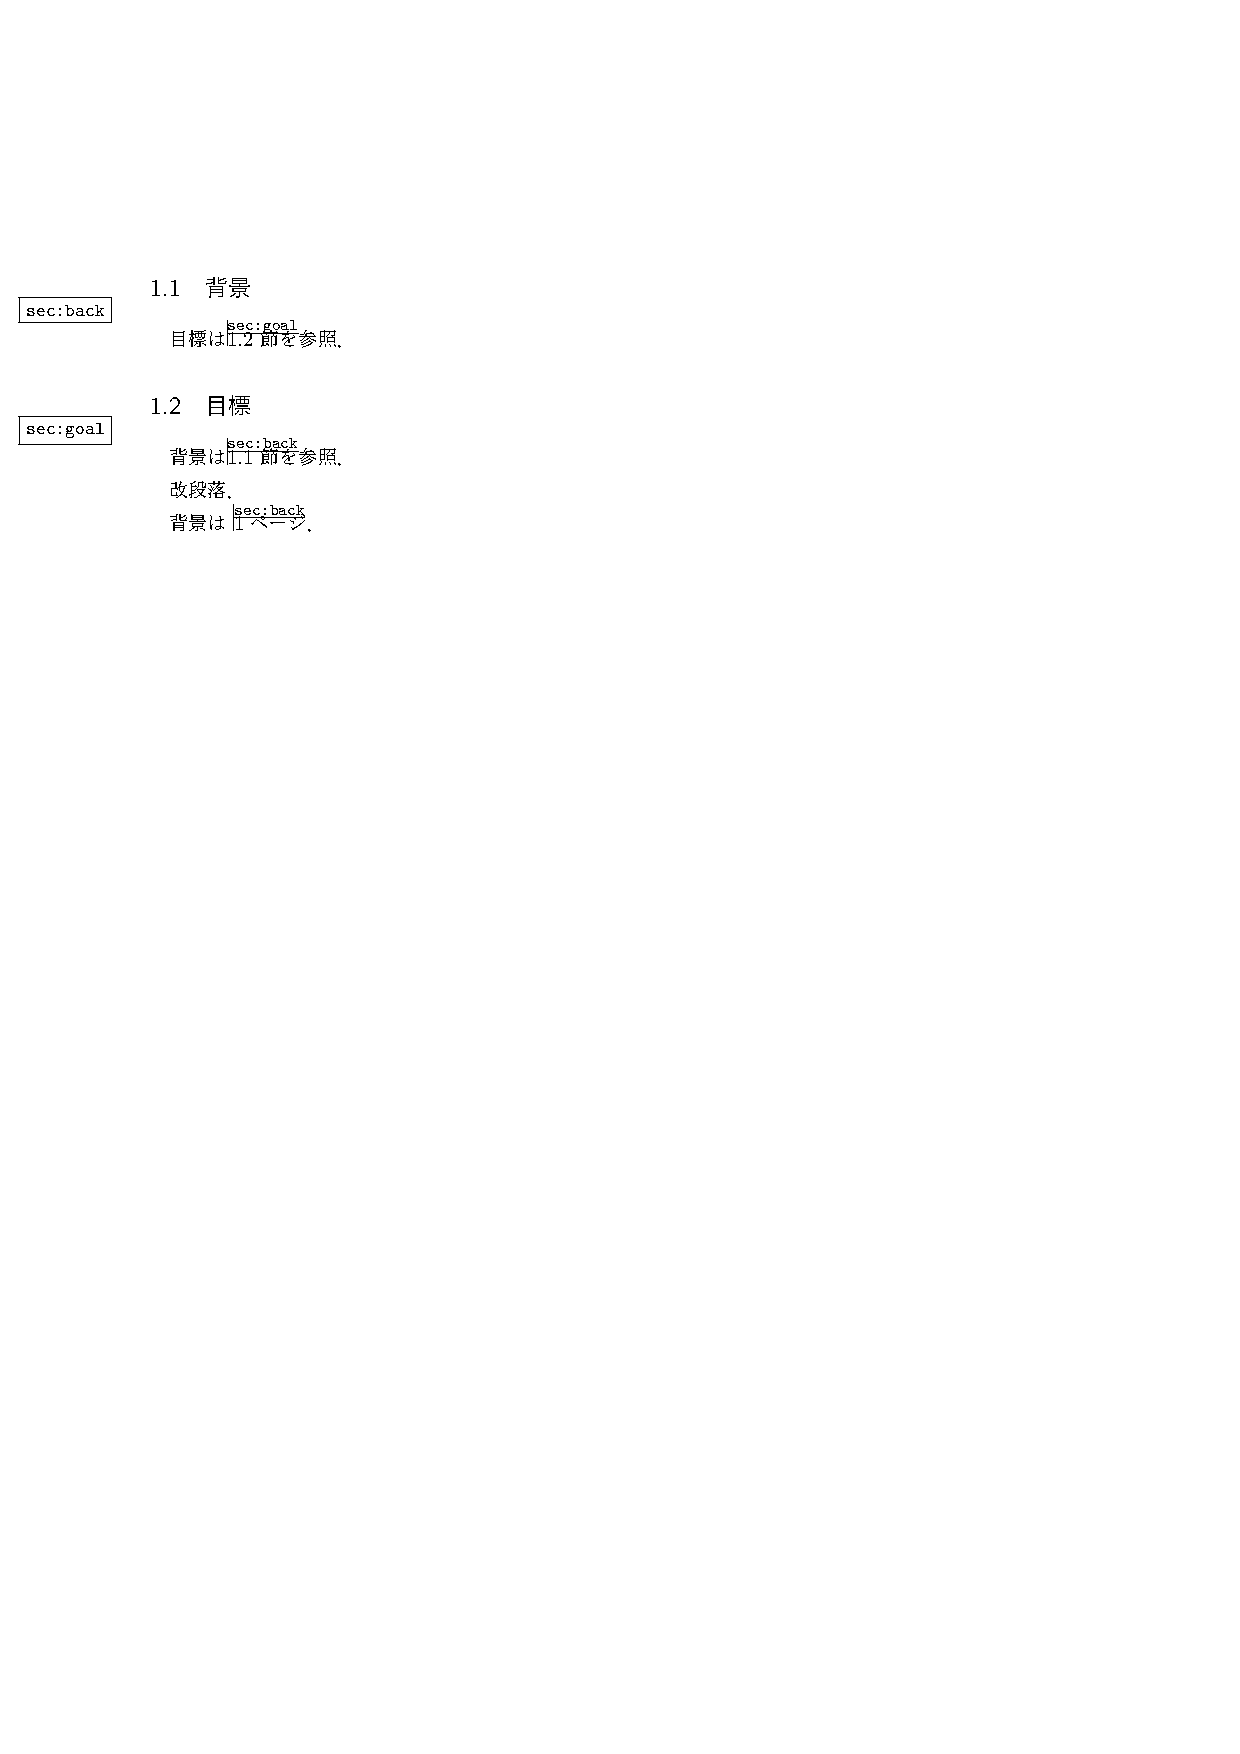
\includegraphics[clip,viewport=8 585 165 710]{images/showkeys}}}
\end{picture}
\begin{small}
\begin{verbatim}
\usepackage{showkeys}
\section{����}
\subsection{�ط�}\label{sec:back}
��ɸ��\ref{sec:goal}~��򻲾ȡ�
\subsection{��ɸ}\label{sec:goal}
�طʤ�\ref{sec:back}~��򻲾ȡ�\par
�����\par
�طʤ�~\pageref{sec:back}�ڡ�����
\end{verbatim}
\end{small}\IOlabel

\subsection{��߻��Ȥ˴ؤ��\LaTeX �ηٹ�}
%\zindind{��߻���}{�˴ؤ��ٹ�}%
%���ޥ�ɥץ���ץȤ䥷�����ɽ�������\dos{LaTeX Warning:}
%�θ�˰ʲ��˼����褦�ʷٹ�ɽ������Ƥ���ȡ�
%��߻��Ȥ˴ؤ������꤬��ä���Ƥ��ʤ����Ȥ򼨤��ޤ���
%\par\dos{Label `key' multiply defined\hfil}
%�Ȥ����Τ� \cmd{label}̿���Ʊ����٥�̾����ĥ�٥��������Ƥ���
%�Ȥ������ȤǤ�����٥�ν�ʣ������ޤ��Τǡ���������
%��٥���̤�̾�����դ��ޤ���
%
%\par\dos{Reference `key' on page n undefined\hfil}
%�Ȥ����ٹ�ɽ�����줿�Τʤ�Х�٥�̾���������Ƥ��ʤ�
%���Ȥˤʤ�ޤ���
%
%\par\noindent\dos{Label(s) may have 
%changed. Return to get cross-ferecenses right.\hfil} 
%��ɽ�����줿���٥���ͤ��ѹ����줿�Ȥ������ȤʤΤǡ�
%�⤦1�٥����ץ��åȤ򤷤ޤ������κ�Ȥ�1�٤ǽ����ʤ�
%���Ȥ⤢��Τǥ�å�������ɽ������ʤ��ʤ�ޤǥ����ץ��å�
%�򷫤��֤����Ȥ⤢��ޤ���
%
%��٥�˴ؤ�������ϥ�٥�λ��Ȥ���̾���ʤɤΥ��ڥ�ߥ��ʤ�
%��ͤ����ޤ���
\zindind{��߻���}{�˴ؤ��ٹ�}%
���ޥ�ɥץ���ץȤ䥷�����ɽ�������\dos{LaTeX Warning:}
�θ�˰ʲ��˼����褦�ʷٹ�ɽ������Ƥ���ȡ�
��߻��Ȥ˴ؤ������꤬��ä���Ƥ��ʤ����򼨤��ޤ���
\index{���顼!Label `key' multiply defined@\texttt{Label `key' multiply defined}}
\index{Label `key' multiply defined@\texttt{Label `key' multiply defined}}
\par\dos{Label `key' multiply defined\hfil}
�Ȥ����Τ� \cmd{label}̿���Ʊ����٥�̾����ĥ�٥��������Ƥ���
�Ȥ������Ǥ�����٥�ν�ʣ������ޤ��Τǡ���������
��٥���̤�̾�����դ��ޤ���

\index{���顼!Reference `key' on page n undefined@\texttt{Reference `key' on page n undefined}}
\index{Reference `key' on page n undefined@\texttt{Reference `key' on page n undefined}}
\par\dos{Reference `key' on page n undefined\hfil}
�Ȥ����ٹ�ɽ�����줿�Τʤ�Х�٥�̾���������Ƥ��ʤ�
���ˤʤ�ޤ���

\index{���顼!Label(s) may have 
changed. Return to get cross-ferecenses right.@\texttt{Label(s) may have changed. Return to get cross-ferecenses right.}}
\index{Label(s) may have changed. Return to get cross-ferecenses right.@\texttt{Label(s) may have changed. Return to get cross-ferecenses right.}}
\par\dos{Label(s) may have 
changed. Return to get cross-ferecenses right.\hfil} 
��ɽ�����줿���٥���ͤ��ѹ����줿�Ȥ������ʤΤǡ�
�⤦1�٥����ץ��åȤ򤷤ޤ������κ�Ȥ�1�٤ǽ����ʤ�
���⤢��Τǥ�å�������ɽ������ʤ��ʤ�ޤǥ����ץ��å�
�򷫤��֤����⤢��ޤ���

��٥�˴ؤ�������ϥ�٥�λ��Ȥ���̾���ʤɤΥ��ڥ�ߥ��ʤ�
��ͤ����ޤ���


%\begin{metacomment}
% �ʲ��Υޡ������åפˤ����������������褦�ʥ�٥�ˤޤǽ���Ԥ�ȯŸ�Ǥ��ʤ��Ȼפ��Τǡ������ȤȤ��롥
%\end{metacomment}

\begin{comment}

\section{�ޡ������åפˤ������}

���ơ�����ޤ�\laTEX �ˤ����륳�ޥ�ɤι�����ˡ�ȵ�ǽ�������ˤĤ���
���Ƥ������Ǥ��������Τ褦�ʼ��ʤ��󶡤���Ƥ���Ȳ��������Ȥʤ�ΤǤ��礦����

�����\LaTeX �ˤ����ƥޡ������åפˤ�뵭�Ҥ򤹤���ˤ�ꡤ\K{Ǥ�դ����Ǥ�
��̣�դ���Ԥ������Ǥ���}�Ȥ������Ǥ���

\chapref{kousei}�Ǥ�ʸ����κۤ�Ĵ�����륳�ޥ�ɡ��㤨�н��Τ��礭����
�ѹ����� \C{Large}�����Ǥ����·���ˤ��� \Env{center} �Ķ��Ϥɤ��
\K{���Ū���κۤ�ľ���ѹ�����}�Ȥ������ޥ�ɤ�¾�ʤ�ޤ���
���Τ��ᡤ������ľ�ܸ�����ǵ��Ҥ��Ƥⲿ���̣�դ��ޤǤϤ��Ƥ��ʤ���
�ˤʤ�ޤ���

%\begin{Exe}
%���ˤ��ξ줷�Τ�Ū��
%\end{Exe}

\begin{Prob}
���줬�ɤΤ褦�����������������Τ��������絬�Ϥ�ʸ���ɮ���Ƥ����
�ˡ����줬����Ǥ���Ǥ��礦��

�Ϥᤫ��ޥ��������ޤ��ϰ��̲�������ˤ�äƤɤΤ褦������������Τ���
��ʬ�ʤ�˹ͻ����Ƥ���������
\end{Prob}


%\subsection{��̣�ε���}

�⤷��Ǥ�դ����Ǥΰ�̣�ȥ쥤�����Ȥ�Ʊ���˵��Ҥ��褦�Ȼפ��С�
WYSIWYG �����ˤ���ɥץ����å��Ǥ���������ʼ���Ƨ�����
�ʤ�Ǥ��礦�������Ǥΰ�̣���ǧ���ʤ���κ�Ȥ��񤷤��Ǥ��礦��
�������ۤȤ�ɤ� WYSIWYG �����Υ�ɥץ����å��ϻ�Х쥤������
��ͥ�褷������ʸ�Ϥ˽񤫤�Ƥ������Ǥΰ�̣�ޤǤ��İ����ʤ��Τ�
���̤�����Ǥ���

% ��������ʤΤ���
%\LaTeX �Τ褦�ʽ����ϤǤϤ��Τ褦���������Ǥ������Ǥ�
%��̣���ǧ���ʤ��鸶�Ƥ�ɮ���������ǽ�Ǥ���

%\subsection{�����}

%\begin{Exe}
%�絬�Ϥ�ʸ���������褦�Ȼפ���\K{���Ƥ�ɮ�������˰�����˴ؤ���
%�롼�����ꤹ��}ɬ�פ�����Ȥ������Ǥ�\footnote{������������ڤ�����
%�ˤ��ξ줷�Τ�Ū�˥��ߤΥ쥸�����������ʤ���Фʤ�ʤ��Ȥ�������
%�ˤ����ƤϤ��θ¤�ǤϤ���ޤ���}��
%\end{Exe}


%\subsection{�Ѹ������}
%
%\subsection{�����}
%
%��٥뻲�Ȥξ��Ǥ�Ʊ��
\end{comment}

%       4 コマンドとマークアップ
%#!platex -src-specials jou.tex
\chapter{�������}\chaplab{math}
\zindind{����}{������}%
\begin{abstract}
%{\LaTeX}��{\TeX}��١����ˤ������ǥ����ƥ�ʤΤ�
%���������Ǥ����դǤ������ξϤǤϴ���Ū�ʿ�����
%���Ϥλ�����Ҳ𤷤ޤ���
{\LaTeX}��{\TeX}��١����ˤ������ǥ����ƥ�ʤΤ�
���������Ǥ����դǤ������ξϤǤϴ���Ū�ʿ����ν���
�λ�����Ҳ𤷤ޤ����������̾��ʸ�ϤȤϰۤʤä����Ǥ�
�Ԥʤ��ޤ���%���Τ��ᡤ�פ����ʬ�ǥߥ��򤷤Ƥ��ޤ���ǽ����
%����ޤ��Τǡ����ξϤ����տ����ɤ�Ǥ���������
\end{abstract}

\section{�Ϥ����}
%{\LaTeX}����Ѥ������̣�Ͽ��������Ǥ���ȸ��äƤ�
%����ǤϤ���ޤ���%plain {\TeX}�ʤ�С������Ȥ�
%�褦�˿������Ȥ�Ω�Ƥ뤳�Ȥ���ǽ�ǡ����Ϸ�̤�����
%�ǹ�Ȥ�����Ǥ��礦��
%{\LaTeX}�ˤ�����������Ȥ�Ω
%�ƤǤ�{\KY{���롼�ԥ�}}�����פǤ���������������Ǥ����Τ�
%���̤��ޤ������������̤�ʸ�ϤȤϰ㤤�����Ķ��˵���\indindz{����}{����}%
%���ޤ���������ʸ�ϤȤϰۤʤꡤ�ѿ���\Z{���ص���}���黻
%�ҡ�ʬ���ʤɤ��ü�ʵ��Ҥ򤷤ʤ���Фʤ�ʤ�����ˡ�
%����Ū��\yo{�����������Ǥ���}���������ɬ�פ�����%
%\index{�⡼��}\indindz{�⡼��}{����}\indindz{�⡼��}{�ƥ�����}%
%\zindind{����}{�⡼��}%%
%�ޤ���ʸ�Ϥ���ʬ��{\KY{�ƥ����ȥ⡼��}}��
%������ޤ���ʬ��{\KY{�����⡼��}}�ȸƤӤޤ���
%�����⡼�ɤϤɤ����������Ϥ���Ƥɤ��ޤǿ����ˤ�
%�뤫�Ȥ��������Ƚ��������ɬ�פ⤢��ޤ���
%�����⡼�ɤǤϰʲ������󤬤���ޤ���
%\begin{itemize}
%\item  �������ԤϾ�˰�ĤΥ��ڡ����Ȥ���
%�����ޤ����̾��{\LaTeX}¦����ư�Ƕ�����������ޤ���
%�桼��������Ū�˶�����������뤳�Ȥ�Ǥ��ޤ���
%\item  \Z{����}�Ϻ������ޤ��󡥰�Ĥμ����Ф��ư��
%�������񤯤��Ȥ��Ǥ��ޤ���
%\item  Ⱦ�ѱѻ��Ϥ��٤ƻؼ����ʤ��¤����������å���
%\pp{$math\ italic$}�ˤʤꡤ��ưŪ�˶���Ĵ�ᤵ��ޤ���
%\end{itemize}
{\LaTeX}�ˤ�����������Ȥ�Ω�ƤǤ�\KY{���롼�ԥ�}��
���פǤ���������������Ǥ����Τ˶��̤��ޤ������������̤�ʸ�Ϥ�
\indindz{����}{����}%
�ϰ㤤\K{�����Ķ��˵��Ҥ��ޤ�}��������ʸ�ϤȤϰۤʤꡤ
�ѿ���\Z{���ص���}���黻�ҡ�ʬ���ʤɤ��ü�ʵ��Ҥ򤷤�
����Фʤ�ʤ�����ˡ�����Ū��\yo{�����������Ǥ���}��%
\index{�⡼��}%
\indindz{�⡼��}{����}%
\indindz{�⡼��}{�ƥ�����}%
\zindind{����}{�⡼��}%
�������ɬ�פ�����ޤ���ʸ�Ϥ���ʬ��\KY{�ƥ����ȥ⡼��}��
������ޤ���ʬ��\KY{�����⡼��}�ȸƤӤޤ���
�����⡼�ɤϤɤ����������Ϥ���Ƥɤ��ޤǿ����ˤ�
�뤫�Ȥ��������Ƚ��������ɬ�פ⤢��ޤ���
�����⡼�ɤǤϰʲ������󤬤���ޤ���
\begin{itemize}
\indindz{����}{�����⡼�����}%
\indindz{����}{�����⡼�����}%
\item  �������ԤϾ�˰�ĤΥ��ڡ����Ȥ���
�����ޤ����̾��{\LaTeX}¦����ư�Ƕ�����������ޤ���
�桼��������Ū�˶���������������Ǥ��ޤ���
\item  \Z{����}�Ϻ������ޤ��󡥰�Ĥμ����Ф��ư��
�������񤯻����Ǥ��ޤ���
\item  Ⱦ�ѱѻ��Ϥ��٤ƻؼ����ʤ��¤����������å���
\pp{$math\ italic$}�ˤʤꡤ��ưŪ�˶���Ĵ�ᤵ��ޤ���
\end{itemize}


\section{�������}
����������������������{\KY{ʸ�����}}��
�̹Ԥ���������{\KY{�̹Կ���}}��2���ब��
��ޤ���
%��򼨤���$\int_{\alpha}^{\beta}f(x)\ 
%dx={[F(x)]}^{\beta}_{\alpha}=F(\beta )-F(\alpha )$
%��ʸ������Ǥ���
%\[
%  \int_{\alpha}^{\beta}f(x)\ dx=
% {[F(x)]}^{\beta}_{\alpha}=F(\beta )-F(\alpha )
%\]
%���̹Կ����Ǥ���
�̹Կ����ˤ��ֹ��դ����̹Ԥ�
��������\env{equation}�Ķ���ʣ���Ԥ��ֹ��դ�����
����Ϥ���\env{eqnarray}�Ķ��ʤɤ�����ޤ���

\subsection{ʸ�����}\indindz{����}{ʸ��}
ʸ������ν��Ϥˤ�3�̤ꤢ��ޤ���%
\glossary{"(@\hspace*{-1.2ex}\verb+\(+}%"}
\glossary{")@\hspace*{-1.2ex}\verb+\)+}%"}
\index{"$@\verb+$+}%"}
\glossary{"$@\verb+$+}%"}
\begin{Syntax}
%\verb|$����$|  \\
%\verb|\(����\)|\\
%\verb|\begin{math}|����\verb|\end{math}|
\verb|$| \va{����} \verb|$|  \\
\cmd{(} \va{����} \cmd{)}\\
\verb|\begin{math}| \va{����} \verb|\end{math}|
\end{Syntax}
�ɤ��Ʊ���褦��ư��򤷤ޤ�����\qu{\str{$}\va{����}\str{$}}
�ǰϤ��Τ���ñ�Ǥ��ΤǤ�������Ȥ����ɤ��Ǥ��礦��

\Env{math}�Ķ��ʤɤϵ����̤�������ΤǻȤ�ʤ��Ƥ�
�����ޤ��󤬡����ޤ�˿�����Ĺ���ʤ긫�Ť餤�Ȥ��ˤ�
\env{math}�Ķ�������Ҥˤ���Ȥ��ä��ꤹ�뤫���Τ�
�ޤ���
\index{=@\str{=}!����Ȥ��Ƥ�\zdash}%
\begin{InOut}
$a$ ��2��� $b$ ��2���­������Τ�
$c$ ��2����������Ȥ������� 
\( a^2 + b^2 = c^2 \) ��ɽ���뤬 
\begin{math}  a^2 + b^2 = c^2
\end{math} �Ƚ񤯻���Ǥ��롥
\end{InOut}
�嵭����ˤ����ƥϥå�\qu{\string^}��ź������
���դ��ε�ǽ����äƤ��ޤ���

%����Ū�˿��������̤�ʸ�Τ������ˤ�Ⱦ�Ѷ������������Τ������Ǥ��礦��

\subsection{���롼�ԥ�}
\indindz{�ȳ��}{�����⡼�����}%
\indindz{���}{�����⡼�����}%
�ѿ�$a$��$x+y$�����Ϥ��뤿���{\LaTeX}�Ǥ�
��������Ǥ�\K{�ȳ��}��{\KY{���롼�ԥ�}}
���ޤ��������ǤϤ٤������ˤȤäƸ��Ƥߤޤ��礦��
\begin{InOut}
\( a^x+y \neq a^{x+y} \)
\end{InOut}
���롼�ԥ󥰤ˤ�äƿ��������Ǥ��ĤΥ��롼�פˤ�
�ޤ��������Ķ��˸¤�ޤ���{\LaTeX}�Ǥϰ�Ĥˤ���
�����Ǥ򥰥롼�פȤ��ư������ȳ�̤ǥ��롼�ײ���
�Ԥ��ޤ���


\subsection{�̹Կ���}\indindz{����}{�̹�}%

%��������̹Ԥ�Ω�Ƥ���ˡ��{\LaTeX}�Ǥϼ��3�̤ꤢ��ޤ���2004/04/15
�������̹Ԥ�Ω�Ƥ���ˡ��{\LaTeX}�Ǥϼ��3�̤ꤢ��ޤ���
\glossary{[@\hspace*{-1.2ex}\verb+\[+}%
\glossary{]@\hspace*{-1.2ex}\verb+\]+}%
\index{$$@\verb+$$+}%
\begin{Syntax}
%\verb+$$����$$+ \\
%\verb+\[����\]+ \\
%\verb|\begin{displaymath} ����\end{displaymath}|
\verb|$$| \va{����} \verb|$$| \\
\verb|\[| \va{����} \verb|\]| \\
\verb|\begin{displaymath}| \va{����} \verb|\end{displaymath}|
\end{Syntax}
%����黰�Ĥ�̿�������Ǽ�ưŪ�˲��Ԥ����꿷����
%�Ԥ�����������Ϥ���ޤ���ξ���Ȥ���������·%
%\zindind{����}{�κ�·��}\indindz{��·��}{������}%
%\indindz{�ե�����}{ʸ�񥯥饹}%
%����ɽ�����ޤ���������·���ˤ��������ʸ�񥯥�
%���ե�����Υ��ץ�����\Option{fleqn}����ꤷ�ޤ���
%�嵭��ʸ�������Ʊ����\verb+\[����\]+������Ȥä�
%�ۤ�����ñ�Ǥ���\Env{displaymath}�Ķ��ϵ����̤�������
%�ΤǻȤ�ʤ��Ƥ⹽���ޤ��󡥤��ޤ�˿�����Ĺ���ʤä�
%�Ȥ��ʤɤˤϻȤ���Ǥ��礦��
����黰�Ĥ�̿�������Ǽ�ưŪ�˲��Ԥ����꿷����
�Ԥ�����������Ϥ���ޤ���ξ���Ȥ���������·%
\zindind{����}{�κ�·��}\indindz{��·��}{������}%
\indindz{�ե�����}{ʸ�񥯥饹}%
����ɽ�����ޤ���������·���ˤ��������ʸ�񥯥�
���ե�����Υ��ץ�����\Option{fleqn}����ꤷ�ޤ���
�嵭��ʸ�������Ʊ����`\cmd{[} \va{���� }\cmd{]}'������Ȥä�
�ۤ�����ñ�Ǥ���\Env{displaymath}�Ķ��ϵ����̤�������
�ΤǻȤ�ʤ��Ƥ⹽���ޤ��󡥤��ޤ�˿�����Ĺ���ʤä�
�Ȥ��ʤɤˤϻȤ���Ǥ��礦��
%\begin{InOut}
%�̹�Ω�ƿ����� \[ c^2 = a^2 + b^2 \]
%�Τ褦�˼�ưŪ�����·���ˤʤ�ޤ���
%\end{InOut}
%\begin{InOut}
%�̹�Ω�ƿ�����
%\begin{displaymath}
% a^2 + b^2 = c^2
%\end{displaymath}
%�Ƚ񤯤��Ȥ�Ǥ��ޤ���
%\end{InOut}
\begin{InOut}
�̹�Ω�ƿ����� \[ 
        c^2 = a^2 + b^2 
\] �Τ褦�˼�ưŪ�����·���ˤʤ�ޤ���
\end{InOut}

\begin{InOut}
�̹�Ω�ƿ�����
\begin{displaymath}
     a^2 + b^2 = c^2
\end{displaymath}
�Ƚ񤯻���Ǥ��ޤ���
\end{InOut}



\indindz{�ֹ�}{������}%
\subsection{�ֹ��դ�����}\indindz{����}{�ֹ��դ���}%
ʸ�����ǻ��Ȥ���������Ȼפ�������ˤ�
�ֹ���դ��ޤ������Τ褦�ʿ�����{\KY{��
���դ�����}}�ȸƤӡ�������1�Ԥξ���
\Env{equation}�Ķ��ǽ��Ϥ�������Ǥ��ޤ���
\begin{Syntax}
\verb+\begin{equation}+\\
\va{����} \C{label}\pa{��٥�}\\
\verb+\end{equation}+
\end{Syntax}
\Env{equation}�ǰϤ���ˤ��1�Ԥ��ֹ��դ�
�ο�������Ϥ�������Ǥ��ޤ����ֹ��դ��ο�
���ϴ���Ū�˥�٥��Ž������Ǥ��ޤ�����
�٥�λ��Ȥλ�����\secref{xr}�򻲾Ȥ��Ƥ���������
\begin{InOut}
\begin{equation}
 a^2 + b^2 = c^2  \label{eq:equ}
\end{equation}
��~(\ref{eq:equ}) ��� $c^2$ �� 
$a^2+b^2$ ����������
\end{InOut}
%"
\subsection{ʣ���Կ���}\seclab{eqnarray*}

\index{=@\str{=}!eqnarray���󤭤礦�����@\texttt{eqnarray}�Ķ����\zdash}
\begin{Syntax}
%\verb|\begin{eqnarray*}| \\
%\verb|���� & (=) & ����\\| \\
%\verb|���� & (=) & ����| \\
%\verb|\end{eqnarray*}|
\verb|\begin{eqnarray*}| \\
\va{����} \str& \va{�ط���} \str& \va{����} \verb|\\| \\
\va{����} \str& \va{�ط���} \str& \va{����} \\
\verb|\end{eqnarray*}|
\end{Syntax}
ή��Τ���ʣ���Ԥο���������ʤɤǴط��ҡ��㤨������\qu{$=$}�ˤΰ���
��·����Ȥ���\Env{eqnarray*}�Ķ�����Ѥ��������
{\KY{ʣ���Կ���}}�ȸƤӤޤ������δĶ���
Ǥ�դιԿ��ι���˻��Ƥ��ޤ���1�Ԥˤ�\Z{����ѥ����}%
\index{"&@\verb+&+!eqnarray*@\texttt{eqnarray*}�Ķ���\zdash}%}
\glossary{"&@\verb+&+!eqnarray*@\texttt{eqnarray*}�Ķ���\zdash}%}
\index{����!eqnarray���󤭤礦�Ǥ�@\texttt{eqnarray}�Ķ��Ǥ�\zdash}%}
\qu{\str{&}}����Ĥޤǡ��Ԥν����ˤϲ���\qu{\texttt{\bs\bs}}%}}}%}$"}
��񤭤ޤ����������ǽ��Ԥˤϲ��Ԥ�����ޤ���
�ޤ�����ˤ�������ʬ�Ͼ�ά���������ǽ�Ǥ���
\begin{InOut}
\begin{eqnarray*}
f(x)      & = & x^2  \\
f'(x)     & = & 2x   
\end{eqnarray*}
\end{InOut}
%\int f(x) dx & = & x^3/3+C


\begin{Prob}
������������򸫤ơ����줾�����ˡ���ǧ���Ƥ���������

\begin{InOut}
\begin{eqnarray*}
 5c = 4g \\
 6a + 3c + 7d = 2g \\
 3a + 5c = 3g
\end{eqnarray*}
\end{InOut}
%�嵭����ϥ���ѥ����\qu{\string&}�ˤ����ڤ꤬����ޤ��󤬡�
%������Ͱʲ��ν������Ʊ���褦�ʷ�̤�����夤�Ƥ��ޤ���
\begin{InOut}
\begin{eqnarray*}
 5c           &=& 4g \\
 6a + 3c + 7d &=& 2g \\
 3a + 5c      &=& 3g
\end{eqnarray*}
\end{InOut}

\begin{InOut}
\begin{eqnarray*}
&& 5c = 4g \\
&& 6a + 3c + 7d = 2g \\
&& 3a + 5c = 3g
\end{eqnarray*}
\end{InOut}

%\begin{InOut}
%\begin{eqnarray*}
%& 5c &= 4g \\
%& 6a + 3c + 7d &= 2g \\
%& 3a + 5c &= 3g
%\end{eqnarray*}
%\end{InOut}

\begin{InOut}
\begin{eqnarray*}
& 5c = 4g &\\
& 6a + 3c + 7d = 2g &\\
& 3a + 5c = 3g&
\end{eqnarray*}
\end{InOut}

%\begin{InOut}
%\begin{eqnarray*}
% 5c&& = 4g \\
% 6a + 3c + 7d &&= 2g \\
% 3a + 5c &&= 3g
%\end{eqnarray*}
%\end{InOut}

%\begin{InOut}
%\begin{eqnarray*}
%& 5c = 4g \\
%& 6a + 3c + 7d = 2g \\
%& 3a + 5c = 3g
%\end{eqnarray*}
%\end{InOut}

%\begin{InOut}
%\begin{eqnarray*}
% 5c           &= 4g &\\
% 6a + 3c + 7d &= 2g &\\
% 3a + 5c      &= 3g &
%\end{eqnarray*}
%\end{InOut}

\end{Prob}

\begin{Prob}
������������������ȡ��ɤΤ褦�ʥ��顼��ɽ������뤫��ǧ���Ƥ���������
���η�̤���ɤΤ褦�ʻ���������Ǥ��礦����

\begin{InTeX}
\begin{eqnarray*}
 & 5c           & = & 4g \\
 & 6a + 3c + 7d & = & 2g \\
 & 3a + 5c      & = & 3g
\end{eqnarray*}
\end{InTeX}

%! LaTeX Error: Too many columns in eqnarray environment.
% �פ���� 3 ��ޤǤ����б����Ƥ��ʤ��Ȥ������������
% rcl �Ȥ���·���ˤʤ�Ȥ�������
\end{Prob}

\subsection{\Z{ʣ�����ֹ��դ�����}}\seclab{eqnarray}
\indindz{����}{ʣ���Ԥ��ֹ��դ�}%
\indindz{�ֹ�}{ʣ���Ԥο�����}%
�夫�黲�Ȥ��������ʣ���Ԥο����ˤ��ֹ���
����Ԥ��ޤ��������{\KY{ʣ�����ֹ��դ�����}}
�ȸƤӡ�\Env{eqnarray}�Ķ���ȤäƵ��Ҥ��ޤ���
�񼰤�\env{eqnarray*} ��Ʊ���Ǥ���
��٥��1�Ԥ��Ȥ˲���\qu{\texttt{\bs\bs}}������Ž�뤳
�Ȥ��Ǥ��ޤ����ޤ��ֹ����Ϥ������ʤ��Ԥ� \Cmd{nonumber}̿��
�ˤ�ä��ֹ�򿶤�ʤ�����Ǥ��ޤ���
\begin{InOut}
\begin{eqnarray}
f(x)       &=& x^2 \label{eq1}\\
f'(x)      &=& 2x  \label{eq2}\\
\int f(x)dx&=& x^3/3+C\nonumber
\end{eqnarray}
��~(\ref{eq1}) ����ʬ������Τ�
��~(\ref{eq2}) �Ǥ��롥
\end{InOut}
 
ʣ���Կ����Ϥ��Ǥ˿����⡼�ɤˤʤäƤ��ޤ��Τ�
����򤵤�˿����Ķ��ǰϤ�ʤɤν����򤷤ʤ���
����������\env{eqnarray*} �Ķ���Ʊ�ͤ˺ǽ��Ԥ˲��Ԥ�����ʤ��Ǥ���������


\section{���Τ��ѹ�}\zindind{����}{�ν��Τ��ѹ�}%
�����ǤϽ��Τ��ѹ���ɬ�פˤʤ�Ȼפ��ޤ���
�㤨�й����ɽ����Τϥܡ�����Τ��ѹ����������
ʸ����ɽ������Ȥ�������Ǥ��礦�����Τ褦�ʤȤ���
�����ѹ��ѤΥ��ޥ�ɤ�Ȥ��ޤ���������Ǥ�
�̾�Υƥ����ȥ⡼�ɤǻȤ������ѹ����ޥ�ɤ�
�Ȥ��ޤ���Τǡ������ν����ѹ��ѤΥ��ޥ�ɤ�
�Ȥ��ޤ���������Ǥ������ѤǤ��ʤ������ѥ���
��ɤ�\tabref{mathfont}���̤�Ǥ���
\begin{table}[htbp]
\begin{center}
\caption{�����⡼�ɤˤ�������Τ��ѹ�}\tablab{mathfont}
\begin{tabular}{lll}
\TR
\Th{����}          & \Th{̿��} & \Th{����} \\
\MR
ɸ��ν���    & \Cmd{mathnormal} & $\mathnormal{ABCabc}$ \\
�����ޥ���    & \Cmd{mathrm}     & $\mathrm{ABCabc}$ \\
���󥻥����  & \Cmd{mathsf}     & $\mathsf{ABCabc}$ \\
�����ץ饤����& \Cmd{mathtt}     & $\mathtt{ABCabc}$ \\
�ܡ������    & \Cmd{mathbf}     & $\mathbf{ABCabc}$ \\
��������  & \Cmd{mathit}     & $\mathit{ABCabc}$ \\
���ꥰ��ե��å���& \Cmd{mathcal}& $\mathcal{ABC}$\\
\BR
\end{tabular}
\end{center}
\end{table}
\begin{InOut}
\begin{displaymath}
\int f(x) dx \neq 
  \int f(x) \mathrm{d}x
\end{displaymath}
\end{InOut} 
�����ɽ������Τ�\Z{�֥�å��ܡ��ɥܡ������}\pp{\Z{����������}}
��Ȥ��������뤽���Ǥ��������ʸ������ȴ���ˤʤ�
�ܡ�����Τ������Ǥ������ʬ����䤹���ʤäƤ�
�ޤ��������Ȥ��ˤ�\Sty{amssymb}���ɤ߹��ߤޤ���
��������̾�Υƥ����Ȥ�Ȥ������Ȥ���
\Sty{amsmath}�ѥå��������ɤ߹��� \Cmd{text}̿���
�Ȥ��ޤ���\tabref{blackboldfamily}�ˡ�
\begin{table}[htbp]
\begin{center}\zindind{����}{�����ʸ��}%
\caption{\textsf{amssymb}�ˤ��������Τγ�ĥ}\tablab{blackboldfamily}
\begin{tabular}{lll}
\TR
\Th{����} & \Th{̿��} & \Th{����} \\
\MR
�ե饯�ȥ�������         &
 \Cmd{mathfrak} & $\mathfrak{ABCabc}$\\
�֥�å��ܡ��ɥܡ������ & 
 \Cmd{mathbb}   & $\mathbb{ABC}$  \\
������ƥ�����  & 
 \Cmd{text}   & $\text{ABC�����Ǥ�}$    \\
\BR
\end{tabular}
\end{center}
\end{table}

%\[ x\in \mathbf{R} \neq x\in \mathbb{R} \]
\begin{InOut}
\usepackage{amssymb}
$$ x \in \mathbf{R} \neq 
  x \in \mathbb{R}$$
$$ f(x) = 1/(1 + g(x)), (x = 3 
  \text{�Ȥ���})$$
\end{InOut}

\begin{Exe}
�ʲ���������ν�������ͤ��Ʋ�������
% URL:   \url{http://www-cs-staff.stanford.edu/~knuth/things.html}.
% ISBN:  1575863278 (japanese translation: 4434036173).
% Title: \emp{Things a Computer Scientist Rarely Talks About}.
% Page:  170.

\begin{InOut}
\begin{displaymath}
 \bigotimes^n x \stackrel{\mathrm
 {def}}{=} \overbrace{x \otimes (x 
\otimes (\dots \otimes x)\dots)}
  ^{n copies of x}
\end{displaymath}
\end{InOut}

�ºݤˤ� `$n copies of x$' �ˤ����Ƥ� `copies of'
�Ȥ����Τ�ʸ�Ϥˤʤ�٤��Ǥ����顤\C{text}���ޥ�ɤ�Ȥ��Τ�
�ɤ��Ǥ��礦�ʤ����� $x$ �� $n$ �Ͽ����ˤʤ�ޤ��ˡ������ \cmd{dots} ��
�������ɽ���򤷤Ƥ��ޤ���������Ū�ˤ����Ǥ� \cmd{cdots} ̿���Ȥ�
��ˡ���ͤ����ޤ�����äƽ��������������ϼ��Τ褦�ˤʤ�ޤ���

\begin{InOut}
\begin{displaymath}
 \bigotimes^n x \stackrel{\mathrm
 {def}}{=} \overbrace{x \otimes (x
 \otimes (\cdots \otimes x) \cdots)}
   ^{\text{$n$ copies of $x$}}
\end{displaymath}
\end{InOut}
\end{Exe}


\section{�����ˤ���������Ĵ��}
%\zindind{����}{��ζ����Ĵ��}%
%�����⡼�ɤǤ����Ϥ���Ⱦ�Ѷ���ȿ�Ǥ���ޤ���
%{\LaTeX}�Ͽ����⡼�ɤǤϼ�ưŪ���٤�礦����
%�������٤��������Ƥ��ޤ����Ǥ����桼��������
%��Ĵ�ᤷ���ۤ������˸������礬����ޤ���%���Τ褦�ʤȤ���
%�桼��¦�Ƕ����Ĵ�᤹�뤿��\tabref{mathspaces}��
%���ޥ�ɤ�Ȥ��ޤ���
\zindind{����}{��ζ����Ĵ��}%
\zindind{����}{��Ĵ��}%
�����⡼�ɤǤ����Ϥ���Ⱦ�Ѷ���ȿ�Ǥ���ޤ���{\LaTeX}��
�����⡼�ɤǤϼ�ưŪ���٤�礦��������\pp{���ȥ�}�����������٤�������
��Ƥ��ޤ����Ǥ����桼���������Ĵ�ᤷ���ۤ���������ɽ���ˤʤ��
��������ޤ����桼��¦�Ƕ����Ĵ�᤹�뤿��
\tabref{mathspaces}�Υ��ޥ�ɤ�Ȥ��ޤ���
��ʬ\qu{$\int$}������ʬ\qu{$dx$}�Τ������ˤ�
�桼��������������Ȱ�̣Ū���������ʤ�ޤ�\footnote{����ʤ�С�
���ܤ��� \C{,}, \C{:}, \C{;}, \cmd{!} ��
���줾�� \C{thinmuskip}, \C{medmuskip}, \C{thickmuskip}, 
��� \C{thinmuskip}�Ȥ��������Ʊ���Ǥ��ꡤ�����ˤ����Ƥ����̤�
ñ��`mu'���Ȥ��Ƥ���Ȥ����������򤹤�Τ��ɤ��ΤǤ��礦����
�ܽ�ǤϤ�����ʬ�ޤǸ��ڤ��ޤ���}��
\begin{table}[htbp]
\begin{center}
\caption{�����ˤ�������������}\tablab{mathspaces}
\glossary{" @\hspace*{-1.2ex}\verb*+"\" +}%"
\glossary{" @\hspace*{-1.2ex}\verb+"\"!+}%"
\begin{tabular}{*4l}
\TR
\Th{������礭��} & \Th{̿��} & \Th{������} & \Th{������}\\
\MR
����ʤ�         & \verb*| |  & \verb*|dx dy|  
   & $dx dy$ \\
���ʤ꾮�������� & \C{,}    & \verb|dx\, dy| 
   & $dx\, dy$ \\
����������       & \C{:}    & \verb|dx\: dy| 
   & $dx\: dy$ \\
��������������   & \C{;}    & \verb|dx\; dy| 
   & $dx\; dy$ \\
Ⱦ�Ѥζ���       & \verb*+\ + & \verb*|dx\ dy|  % Ŭ�ڤ�ñ��ֶ���
   & $dx\ dy$ \\
���Ѥζ��� (1\,em)      & \C{quad} & \verb|dx\quad dy|
   & $dx\quad dy$ \\
���Ѥ�2�ܤζ��� (2\,em)  & \C{qquad}& \verb|dx\qquad dy| 
   & $dx\qquad dy$ \\
����������   & \cmd{!}     & \verb|dx\!dy|
   & $dx\! dy$ \\
\BR
\end{tabular}
\end{center}
\end{table}

��ʬ\qu{$\int$}������ʬ\qu{$dx$}�Τ������ˤ�
�桼��������������ȸ��Ǥ������ޤ���
\begin{InOut}
\[ \int\int f(x)dxdy \neq 
   \int\!\!\!\int f(x)\ dx\ dy  \]
\end{InOut}


\begin{Exe}
ʣ���μ���1�Ԥ���󤹤��硤���Τ褦�ˤ����
Ŭ�ڤʶ�����������ޤ���
\begin{InOut}
������ $c, v, e$ ��ͤ���Ȥ���
\[c = f_1 + f_2, v = 3f_2 + 
      f_3, e = 2f_1 + 3f_3 \]
\end{InOut}

������θ����ȡ�`\verb|$c, v, e$|'����ʬ�ˤ�Ŭ�ڤ�ñ��ֶ���
����������Τ�˾�ޤ����Ǥ��礦���� \C{quad} ���٤ζ����򤽤줾���
���Τ���������������Τ�Ŭ�ڤ��Ȼפ��ޤ���
\begin{InOut}
������ $c$, $v$, $e$ ��ͤ���Ȥ���
\[c = f_1 + f_2,\quad v = 3f_2
 + f_3, \quad e = 2f_1 + 3f_3 \]
\end{InOut}

\end{Exe}


\begin{Exe}
���Τ�����˾�����򵭽Ҥ���Ȥ���ñ�˴ݳ�̤���
�ĤŤ�����⡤\C{quad}���٤ζ�������������Τ�
�ɤ��Ǥ��礦��

\begin{InOut}
\[ g = \frac{1}{5}a + \frac{1}{6}b 
     \quad (a>3,\ b>5) \]
\end{InOut}

����ˡ���郎ʣ������Ȥ��� \verb*+\ + �ˤ�ꤢ�����٤�
�������������Τ��ɤ��Ǥ��礦��
\end{Exe}

\section{����Ū�ʿ������ޥ��}
������񤯴Ķ������򤷤���ºݤˤ����˵��Ҥ���
����ʤɤ�Ф�����ˤʤ�ޤ���
%�����Ķ��Ǥ�̿
%��Τ�������ˤ�Ⱦ�Ѥζ���������褦�˿�����
%�ޤ��礦���פ�̽�ǥ��顼�ˤʤ��ǽ�������뤿
%�ᥳ�ޥ�ɤ����������齬��Ū�˶���������褦
%�ˤ��Ƥ���������������̿��Τ�������ˤ���ľ��
%�����Ǥ򲿤餫�η��ǽ�������Ȥ��϶�������Ϥ���
%����

\subsection{ź����}\seclab{soeji}
\indindz{ź����}{���դ���}\indindz{ź����}{���դ���}%
{\LaTeX}�Ǥ�\Z{ź����}�����Ϥϴ�ñ�Ǥ���%"
\index{"^@\verb+^+}%
\index{"_@\verb+_+}%
\glossary{"^@\verb+^+}%
\glossary{"_@\verb+_+}%
\begin{Syntax}
\va{��������}\str{^}\pa{���դ�ʸ��} \\
\va{��������}\str{_}\pa{���դ�ʸ��}
\end{Syntax}
ź�����ˤ�{\KY{���դ�}}��{\KY{���դ�}}
��2���ब����ޤ���������ź������Ȥ��ˤϥ��롼�ԥ�
����ɬ�פ�����ޤ���1ʸ��������ź�����ΤȤ��˴ݳ�̤�ɬ
�פ���ޤ��󤬡�ź�����ˤ�������Τ�ʣ���ΤȤ��ϥ��롼��
�󥰤ν�����ɬ�פǤ���\tabref{soeji}����򼨤��ޤ�
�Τǻ��ͤˤ��Ƥ���������ź�������դ���Ȥ��˾��դ��Ȳ���
���ν��֤ϴط�����ޤ���
\begin{table}[htbp]
\begin{center}
\caption{ź�����λȤ�������}\tablab{soeji}
\begin{tabular}{lll|lll}
\TR
\Th{��̣} & \Th{̿��} & \Th{����} & \Th{��̣} & \Th{̿��} & \Th{����}\\
\MR
����       & \verb|x^{a+b}|      & $x^{a+b}$       & 
����       & \verb|{}^{a+b}x|    & ${}^{a+b}x$     \\
����       & \verb|x_{a+b}|      & $x_{a+b}$       & 
����       & \verb|{}_{a+b}x|    & ${}_{a+b}x$     \\
����ȱ��� & \verb|x^{a+b}_{c+d}|& $x^{a+b}_{c+d}$ & 
����Ⱥ��� & \verb|{}^{a}_{b}x|  & ${}^{a}_{b}x$   \\
������ & \verb|x^{a^{b}}|    & $x^{a^{b}}$     &
�����ȱ���& \verb|{}_{a}x_{b}|  & ${}_{a}x_{b}$   \\%$
\BR
\end{tabular}
\end{center}
\end{table}
ź�����ϲ���ʤ���Τ��Ф��Ƥ�ź���������ǽ�Ǥ���
\tabref{soeji}�Ǥ⤽����ˡ���Ȥ��Ƥ��ޤ���
\begin{InOut}
\( {}^{a+b}_{x+y}A^{a+b}_{x+y} \)
\end{InOut}
�ϥå�\qu{\string^}�䥢������С�\qu{\string_}��
�̤�̿��Ȥ��Ƥ��Ѱդ���Ƥ��ޤ������դ��� \Cmd{sp}
�Ȳ��դ��� \Cmd{sb}̿���Ȥ��Ȼ���Ǥ��ޤ���
\begin{InOut}
\( A^4_3 \neq A\sp4\sb3 \)
\end{InOut}

�ʾ�Τ褦����ˡ�ǤϺ�¦��ź�������դ���Ȥ���
���ޤ������ʤ���礬����ޤ��Τǡ�\Person{Harald}{Harders}
�ˤ��\Sty{leftidx}�ѥå�������Ȥ��ޤ���
\begin{Syntax}
\Cmd{leftidx}\pa{��¦ź����}\pa{����}\pa{��¦ź����}\\
\Cmd{ltrans}\pa{����}
\end{Syntax}

\Z{�ִ�����}�ξ��դ�ź�����ϼ㴳������ޤ��뤿��� \Cmd{ltrans}
̿���Ȥ��ޤ���
\begin{InOut}
\begin{eqnarray*}
{}_a^b\left(\frac{x}{y}\right)_c^d 
  &\neq& \leftidx{_a^b}{\left(
    \frac{x}{y} \right)}{_c^d}\\
{}^\mathrm{t} A &\neq& \ltrans{A}
\end{eqnarray*}
\end{InOut}


\subsection{���شؿ�}
�����⡼�ɤǤϼ�ưŪ�˱ѻ���������å��Τˤʤ�ޤ���
������ѿ���ɽ������Ǥ���\qu{$d$}��\qu{$\mathrm{d}$}
�Ͽ����Ǥϰ㤦��̣������ޤ���\Z{���شؿ�}��˸¤ʤɤ�
\K{�����ޥ���}���ޤä����ʽ��Τǽ񤯤Τ����路�Ǥ���
{\LaTeX}�ǤϤ��餫���᤽�Τ褦�ʴؿ�����������
���ꡤ�����˻Ȥ���̿���\tabref{suugakukannsuu}���̤�Ǥ���
\begin{table}[htbp]
\begin{scenter}
 \caption{��ʿ��شؿ�}\tablab{suugakukannsuu}
 \begin{tabular}{LCCCC}
 \M{arccos} & \M{cot}  & \M{exp} & \M{liminf} & \M{sec}  \\
 \M{arcsin} & \M{coth} & \M{gcd} & \M{limsup} & \M{sin}  \\
 \M{arctan} & \M{csc}  & \M{hom} & \M{log}    & \M{sinh} \\
 \M{arg}    & \M{deg}  & \M{inf} & \M{max}    & \M{sup}  \\
 \M{cos}    & \M{det}  & \M{ker} & \M{min}    & \M{tan}  \\
 \M{cosh}   & \M{dim}  & \M{lim} & \M{Pr}     & \M{tanh} \\
 \end{tabular}
\end{scenter}
\end{table}
%
\begin{InOut}
\[cos^2x+sin^2x \neq \cos^2x+\sin^2x\]
\end{InOut}
�ޤ� \Cmd{bmod} �Τ褦��{\KY{ˡ}}��
ɽ�������̿��⤢��ޤ���\indindz{�黻��}{���}%
\begin{Syntax}
\Cmd{bmod}\pa{ʸ����} (\Z{���黻��}�Ȥ���)\\
\Cmd{pmod}\pa{ʸ����} 
\end{Syntax}
\begin{InOut}
\( \mathrm M\bmod{\mathrm N} \neq 
   \mathrm M\pmod{\mathrm N} \)
\end{InOut}

\subsection{�礭�����Ѥο��ص���}
������ǤϽ��������Τˤ�ä��礭����
�Ѥ�뵭�椬����ޤ���\Z{��ʬ����}�ʤɤ�\indindz{����}{��ʬ}%
����ˤ�����ޤ�������礭�������Ѥʵ����\indindz{����}{�礭�������Ѥ�}%
\tabref{kahensushiki}���̤�Ǥ���
\begin{table}[htbp]
\begin{center}
\caption{�礭�����Ѥο��ص���}\tablab{kahensushiki}
\begin{tabular}{lll}
\TR
\Th{����} & \Th{̿��} & \Th{������}\\
\MR
\Z{ʬ��}           & \Cmd{frac}\pa{ʬ��}\pa{ʬ��}&
  $\displaystyle \frac{\text{ʬ��}}{\text{ʬ��}} $ \\[5pt]
����           & \Cmd{sqrt}\pa{��}&
  $\displaystyle \sqrt{\text{��}} $ \\[5pt]
ź�����դ����� & \cmd{sqrt}\opa{��}\pa{��}&
  $\displaystyle \sqrt[\text{��}]{\text{��}}$ \\[5pt]
ź�����դ���ʬ & \cmd{int}\verb|^|\pa{���դ�}%
  \verb|_|\pa{���դ�} &
  $\displaystyle \int^{\text{���դ�}}_{\text{���դ�}} $ \\[5pt]
ź�����դ����� & \cmd{sum}\verb|^|\pa{���դ�}%
  \verb|_|\pa{���դ�} &
  $\displaystyle \sum^{\text{���դ�}}_{\text{���դ�}} $ \\[5pt]
\BR
\end{tabular}
\end{center}
\end{table}
\begin{InOut}
\begin{displaymath}
\int^b_a f(x) dx \neq 
  \sqrt{\frac{1}{f(x)}}
\end{displaymath}
\end{InOut}
\begin{InOut}
\begin{displaymath}
\sqrt{\frac{1}{g(x)} + 
   \sqrt{\int f(x) dx}}
\end{displaymath} 
\end{InOut}
\begin{InOut}
\begin{displaymath}
\frac{1}{g(x)} + 
  \frac{1}{2x^3 + 5x^2 + 8x + 5}
\end{displaymath} 
\end{InOut}
\cmd{sum} �� \cmd{int}�ʤɤ�ź�����Ͼ岼���դ�����
����ȱ������դ���礬����ޤ��������
�ѹ�����ˤ� \Cmd{limits} �� \Cmd{nolimits}��Ȥ��ޤ���
\begin{Syntax}
\begin{tabular}{llll}
 \cmd{limits} &\pp{�岼���դ�} & \cmd{nolimits} &\pp{�����դ�}\\
\end{tabular}
\end{Syntax}
\cmd{limits}��ź������Ԥ����ޥ�ɤ������֤���
ź�����򤵤�뵭��ξ岼��ź������ɽ�����ޤ���\indindz{����}{ź�����ˤ�����}%
\cmd{nolimits}�Ϥ���ȿ�Фλ��򤷤ޤ���
\begin{InOut}
\begin{eqnarray*}
\sum\nolimits^n_{k=0}k & \neq & 
   \sum^n_{k=0}k\\
\int^b_a dx & \neq &
   \int\limits^b_a dx
\end{eqnarray*}
\end{InOut}
%
\begin{InOut}
\begin{eqnarray*}
\lim\nolimits_{n\rightarrow0}n 
  &\neq& \lim_{n\rightarrow0}n \\
\prod^n_{i=1}n &\neq& 
   \prod\nolimits^n_{i=1}n
\end{eqnarray*}
\end{InOut}
 
\subsection{���ڤ국��ȳ��}\seclab{brace}\index{���ڤ�}
\indindz{����}{���ڤ�}\zindind{���ڤ�}{����}%
{\LaTeX}�ˤ�����{\KY{���ڤ국��}} (\Z{���}��ޤ�) 
�ϲ�����ꤷ�ʤ���о�����礭�����Ѥ��ޤ���
���ڤ국���
\begin{itemize}
 \item \Cmd{left}�� \Cmd{right}̿���Ȥä��礭�����Ѥ��롥
 \item ���ڤ국����礭������ꤹ�롥
\end{itemize}
�Ȥ�����Ĥ���ˡ�ˤ�ä��礭�����ѹ��������Ǥ��ޤ���
\begin{InOut}
\begin{displaymath}
\left[ \Big(x+y\Big) \right]
\end{displaymath} 
\end{InOut}
��̤dz��줿�ꡤ���ڤ������Ǥ˱������礭����
�ѹ��Ǥ�����ڤ국���\tabref{brace1}��
�ʤ�ޤ���
\begin{table}[htbp]
\begin{scenter}
\caption{��ʶ��ڤ국��}\tablab{brace1}
\glossary{"{1"}@\hspace*{-1.2ex}\protect\bgroup\verb+"\"{+"}}%
\glossary{"{2"}@\hspace*{-1.2ex}"{\verb+"\"}+\protect\egroup}%
\glossary{"|@"\hspace*{-1.2ex}"\verb+"\"|+}%}
\index{"(@\verb+(+}%"
\index{")@\verb+)+}%
\index{"[@\verb+[+}%
\index{"]@\verb+]+}%
\index{"|@\texttt{\symbol{'174}}}%""
\begin{tabular}{LCCC}
$($ &\verb+(+ & \M{rfloor}   & \M{updownarrow}& \M{lbrace}\\
$)$ &\verb+)+ & \M{lfloor}   & \M{Uparrow}&     \M{rceil}\\
$[$ &\verb+[+ & \M{arrowvert}& \M{Downarrow}&   \M{lceil}\\
$]$ &\verb+]+ & \M{Arrowvert}& \M{Updownarrow}& 
 $\big\lmoustache$&\BM{lmoustache}~${}^*$\\
$\{$&\verb+\{+& \M{Vert}&      \M{backslash}&   
 $\big\rmoustache$&\BM{rmoustache}~${}^*$\\
$\}$&\verb+\}+& \M{vert}&      \M{rangle}&      
 $\big\lgroup$&\BM{lgroup}~${}^*$\\
$|$ &\verb+|+ & \M{uparrow}&   \M{langle}&      
 $\big\rgroup$&\BM{rgroup}~${}^*$\\
$\|$&\verb+\|+& \M{downarrow}& \M{rbrace}&      
 $\big\bracevert$&\BM{bracevert}~${}^*$
\end{tabular}
\\ {\small${}^{*}$\ �緿�ζ��ڤ국��Ǥ���}
\end{scenter}
\end{table}
%}}}"
��̤ʤɤ����Ǥ���ڤ뤿��ε���ǡ����Ǥ򤭤����
���٤��Ǥ���{\LaTeX}�ˤ����Ƥ��礭�������Ѥʶ���
�국����Ѥ��Ƥ������ɽ���ޤ���\qu{\Cmd{left}}
̿���\qu{\Cmd{right}}̿����ФǻȤ��ȳ��줿����
��Ŭ�ڤ��礭���γ�̤Ƕ��ڤ��ޤ���\cmd{left}�� \Cmd{right} ��
��\tabref{brace1}���鵭���
���ֻ��ˤ�äơ������ζ��ڤ���Ф�ͳ���Ȥ߹��
�����ޤ������Ѥγ�̤Ͻ������뼰�ˤ�äƼ�ưŪ��
�礭�����ѹ������ΤǤȤƤ������Ǥ���

\begin{InOut}
\begin{displaymath}
\left( \frac{1}{1+\frac{1}{1+x}} \right) 
\end{displaymath}
\end{InOut}

%\begin{InOut}
%\[ \left\lmoustache \left\{ 
%  \left(\frac{1}{x}+1\right)
%  +\left(\frac{1}{x^2}+2\right) 
%\right\} \right\rmoustache \]
%\end{InOut}

\begin{InOut}
\begin{displaymath}
 \left\uparrow \int f(x)dx 
   \right\downarrow + \left\lgroup 
     \int g(x)dx \right\rgroup
\end{displaymath}
\end{InOut}

\zindind{���}{���礭����Ĵ��}%
��ʬ�dz�̤��礭������ꤹ�����Ǥ��ޤ���
�礭������ꤷ�����Ϥ���ʾ��̤��礭����
�Ѥ��ޤ���Τ����դ�ɬ�פǤ�\pp{\tabref{ookiikakko}}��
\begin{table}[htbp]
\begin{scenter}
\caption{��̤��礭������ꤹ����}\tablab{ookiikakko}
%\index{"/@"\verb+"/+}
\index{"/@"\verb+"/+}%
\index{"/@"\verb+"/+!���ڤ국���\zdash}%
%"
\begin{tabular}{LCCCC}
%\newcommand{\m}[1]{$#1$&\texttt{\string#1}}
\m{/}      & \m{(}       & \m{)}       & \m{|}       &
  $\|$      & \verb+\|+\\
\m{\big/}  & \m{\bigl(}  & \m{\bigr)}  & \m{\bigm|}  &
  $\bigm\|$ & \verb+\bigm\|+\\[4pt]
\m{\Big/}  & \m{\Bigl(}  & \m{\Bigr)}  & \m{\Bigm|}  &
  $\Bigm\|$ & \verb+\Bigm\|+\\[5pt]
\m{\bigg/} & \m{\biggl(} & \m{\biggr)} & \m{\biggm|} &
  $\biggm\|$&  \verb+\biggm\|+\\[6pt]
\m{\Bigg/} & \m{\Biggl(} & \m{\Biggr)} & \m{\Biggm|} &
  $\Biggm\|$&  \verb+\Biggm\|+\\[7pt]
\end{tabular}
\end{scenter}
\end{table}
%
\begin{InOut}
\begin{displaymath}
\Biggl\| \Biggl(\int f(x) dx\Biggr) 
  \Bigg/ \Biggl(\int g(x) dx\Biggr) 
\Biggr\| 
\end{displaymath}
\end{InOut}
\tabref{ookiikakko}�򸫤��ʬ����Ȼפ�
�ޤ�������̡���������ڤ국����Ф��� \Cmd{big}
�� \Cmd{Big}���դ���Ȥ��ζ��ڤ�
������������Ψ�dz��礹��Ȥ�����ǽ����\indindz{����}{���ڤ국���}%
��ޤ�����¦����ڤ�ˤ� \Cmd{bigl}���
�ط��ҤȤ��Ƥζ��ڤ국��� \Cmd{bigm}��򡤱�
¦����ڤ뵭��ˤ� \Cmd{bigr}����ä˻���
���ʤ��ʤ�� \Cmd{big}���Ȥ��褦�ˤ��ޤ���
�嵭�� \cmd{big}���Ȥä���� \cmd{left}
�� \cmd{right}�ˤ�������٤Ƥ���������
\begin{InOut}
\[ \left\| 
 \left(\int f(x) dx\right) 
 \Bigg/ \left(\int g(x) dx\right) 
 \right\| \]
\end{InOut}
���������˶��ڤ국�椬������ɤ��Ȥ��ϥԥꥪ��\qu{\str.}��
�����줫�ε�����ά�Ǥ��ޤ���
\begin{InOut}
\[ \left( \left\uparrow 
   \int f(x)dx + \int g(x)dx
   \right. \right) \] 
\end{InOut}

\subsection{����}\seclab{math:array}
{\LaTeX}�ˤ���������\Env{array}�Ķ����
���Ҥ��ޤ���\env{array}�Ķ��Ϥ��ΤޤޤǤ�
�����ˤϤʤ餺\env{math}�Ķ���\verb+\[\]+��
������줿��\verb+$$+���������Ƥ����ޤ���
\texttt{array}�Ķ��δ���Ū�ʻȤ�����
\begin{Syntax}
\verb|\begin{array}|\pa{������}\\
$\begin{array}{cccccc}
\text{��ʬ}_{11} &\verb+&+ & \dots &\verb+&+ & \text{��ʬ}_{1n}  & \verb+\\+\\
\vdots &\verb+&+ & \ddots&\verb+&+ & \vdots  & \verb+\\+\\
\text{��ʬ}_{m1} &\verb+&+ & \dots &\verb+&+ & \text{��ʬ}_{mn}  & 
\end{array}$\\
\verb+\end{array}+
\end{Syntax}
�Ȥ����褦�� $m$ �� $n$ ��ι����񤭤ޤ���
\index{"&@\verb+&+!array@\texttt{array}�Ķ���\zdash}%
\glossary{"&@\verb+&+!array@\texttt{array}�Ķ���\zdash}%
������\Z{����ѥ����}\qu{\texttt\&}����ʬ\pp{����}
�ζ��ڤ���̣����\qu{\texttt{\bs\bs}}�Ϲ�
�ν������̣���Ƥ��ޤ�����̤�ɬ�פʤ��
���Ҥζ��ڤ국��dz�뤳�Ȥ�Ǥ��ޤ���ɽ��
����ϴ���Ū��Ʊ����¤�ǡ��Ĥη����ⲣ�η�
��������뤳�Ȥ��Ǥ��ޤ���\indindz{����}{�����}

\begin{InTeX}
\begin{array}{����Ƚķ����λ���}
\end{InTeX}

������ʬ�Ǥ�4�󤢤�ʤ�м��Τ褦�ˤ��ޤ���

\begin{InTeX}
\begin{array}{lc|cr}
\end{InTeX}

���ΤȤ���\qu{\str l}��\qu{\str c}��
\qu{\str r}�Ϲ����������Ǥ����־�����ꤹ����
�Ǥ���������ˤϥƥ����ȥС�\qu{\texttt |}������ޤ���
����Ͻ������η�����ɽ���Ƥ��ޤ������Τ褦�ʵ����
{\KY{������}}�ȸƤӤޤ���
%\env{array}�Ķ���ǻ���Ǥ��������Ҥ�
%\tabref{math:array}�Ȥʤ�ޤ���
\indindz{������}{����ˤ�����}%
\env{array}�Ķ���ǻ���Ǥ��������Ҥ�
\tabref{math:array}�Ȥʤ�ޤ���
\texttt{array}�Ķ�������Ҥˤ�����⡤
�������˹����񤤤��ꤹ�����Ǥ��ޤ���
%\texttt{array}�Ķ�������Ҥˤ��뤳�Ȥ�Ǥ��ޤ���
%�������˹����񤤤��ꤹ�뤳�Ȥ�Ǥ��ޤ��Τ������Ǥ���

\begin{table}[htbp]
\begin{center}
\indindz{��}{�����}%
\indindz{��}{1���}%
\zindind{����}{����}%
\caption{\texttt{array}�Ķ��μ��������}
\tablab{math:array}
\begin{tabular}{cl}
\TR
 \Th{������} & \Th{��̣}\\
\MR
\str l & ����ν�1���·���ˤ���\\
\str c & ����ν�1������·���ˤ���\\
\str r & ����ν�1���·���ˤ���\\
\verb+|+ & �Ĥη��������\\
\verb+||+ & �Ĥ�2�ŷ��������\\
\str @\pa{ɽ��} & ɽ����1���ɲä���\\
\str p\pa{Ĺ��} & �����������ľ�ܻ��ꤹ��\\
\str *\pa{���}\pa{������} &���ʬ����\va{������}�򷫤��֤�\\
%\verb+l+ & ����ν�1���·���ˤ���\\
%\verb+c+ & ����ν�1������·���ˤ���\\
%\verb+r+ & ����ν�1���·���ˤ���\\
%\verb+|+ & �Ĥη��������\\
%\verb+||+ & �Ĥ�2�ŷ��������\\
%\verb+@{ɽ��}+& ɽ�����1���ɲä��ޤ�\\
%\verb+p{Ĺ��}+& �����������Ĺ����ľ�ܻ��ꤷ�ޤ�\\
%\verb|*{���}{����}|&���ʬ�������ܤ򷫤��֤���\\
\BR
\end{tabular}
\end{center}
\end{table}

%\begin{InOut}
%\[ \left( \begin{array}{cc} 
%      a & b \\ c & d 
%   \end{array} \right) \]
%\end{InOut}

\index{����!array���󤭤礦�Ǥ�@\texttt{array}�Ķ��Ǥ�\zdash}%
�������˹���³����礬���뤿��\env{array}�Ķ���
\K{�Ǹ�ιԤ˲��Ԥ�����ޤ���}��
\begin{InOut}
\[ \left( \begin{array}{*{2}{c}} 
     a & b \\ c  & d 
    \end{array} \right) 
  \left( \begin{array}{c} 
       m \\ n 
    \end{array} \right)  =
  \left( \begin{array}{c} 
      am+bn \\ cm+dn \\ 
    \end{array} \right) \]
\end{InOut}
\index{���ʬ��}%
\env{array}�Ķ��ˤϼ��˼����褦�ʾ��ʬ����Ԥ�
�Ȥ����⤢��ޤ���
\begin{InOut}
\[ f(x)= \left\{
\begin{array}{cl}
  x & (x > 0)\\
  0 & (x = 0)\\
 -x & (x < 0) \end{array} 
\right. \] 
\end{InOut}
%
��ʿ�˷����ʤɤ����줿�ꤹ��Ȥ��ˤ� \Cmd{hline}��
���Ǥ���ǽĤη���������Ȥ��ˤ� \Cmd{vline}�ʤ�
��Ȥ��ޤ�\pp{\tabref{array:lines}}��
�����ʤɤλȤ����ϰʲ�����򸫤����򤷤Ƥ���������

\begin{table}[htbp]
\caption{\texttt{array}�Ķ���Ǥη�����̿��}\tablab{array:lines}
\begin{tabular}{ll}
\TR
 \Th{̿��} & \Th{��̣}\\
\MR
\Cmd{hline}& 
   ���˰���������η���������ޤ�\\
\cmd{hline}\cmd{hline}&
  �����������2�Ť�\Z{������}������ޤ�\\
\Cmd{vline}& 
   ���Ǥ���ǰ���������νķ���������ޤ�\\
\Cmd{cline}\pa{�ϰ�}& 
   ���Ǥη�����Ԥ�\va{�ϰ�}����ꤷ�ư����ޤ�\\
\Cmd{multicolumn}\pa{����} &
   \multirow{2}*{�Ԥ�Ĥʤ���\va{������}�̤�����Ǥ���Ϥ��ޤ�}\\
\multicolumn{1}{r}{\pa{������}\pa{����}} & \\
\BR
\end{tabular}
\end{table}
%

\begin{InOut}
\begin{displaymath}
\begin{array}{llc} \hline
\multicolumn{3}{c}{f(x)} \\ \hline
g(x) & h(x) & i(x) \\ \cline{2-2}
j(x)+k(x)+l(x) & o(x) & p(x)\\
\end{array}
\end{displaymath} 
\end{InOut}

%\begin{InOut}
%\begin{displaymath}
%\newcommand*\MC{\multicolumn}
%\begin{array}{ll|ll}
%a & b & c & d \\ \hline \hline
%e & g & h & i \\ \cline{3-4}
%j & \MC{1}{|l}k & l & m\\ \hline
%n & o & \MC{1}{l|}p & q\\
%r & s & t & \MC{1}{|l|}u\\
%v & w & x & y \\ \hline \hline
%\end{array}
%\end{displaymath} 
%\end{InOut}

%���դ������᤮�ޤ������ʤ���ϩ�ߤ����Ǥ��͡�

\indindz{����}{����դ���}
\env{array}�Ķ��δʰ��ǤȤ��ƹ�������Ѥ� \Cmd{matrix}��
�ݳ�̤��դ��� \Cmd{pmatrix}�� \cmd{matrix}��
��٥���դ����� \Cmd{bordermatrix}�ʤɤ�̿�᤬����ޤ���
������ \cmd{matrix}̿��� \cmd{pmatrix}�˴ؤ��Ƥ�\Sty{amsmath}�ѥå�����
��\Env{matrix}�Ķ���\Env{pmatrix}�Ķ���Ȥä�������
���Ǥ��礦��
\begin{InOut}
\[ \begin{pmatrix} x \\ y 
   \end{pmatrix} \begin{pmatrix}
      a & b & c \end{pmatrix} \]
\end{InOut}

\cmd{bordermatrix}�Ķ��γ�̤Ǥϳ���ʬ����ڤ��
�ϥ���ѥ����\qu{\str\&}��Ȥ����Ԥν����ˤ�
\qu{\Cmd{cr}}̿���Ȥ��ޤ���
\begin{InOut}
\[ A=\ \bordermatrix{
     & 1 & 2 \cr
  1  & a & b \cr
  2  & c & d }     \] 
\end{InOut}


�̤���ˡ�Ȥ��� \Person{David}{Carlisle}�� \Y{delarray} (\Z{delimiter array})
 �ѥå��������Ѥ�����⤢��ޤ������Τ褦�ˤ���� \C{left(} \C{right)} 
����ä�����Ʊ�ͤγ���դ��ˤʤ�ޤ���
\begin{InOut}
\usepackage{delarray}
$\begin{array}({cc})
 a_{11} & a_{12} \\
 a_{21} & a_{22} \\
\end{array}$
\end{InOut}
���Τ褦�˾��ʬ���ΤȤ��ˤ�Ȥ��ޤ���\indindz{���}{���ʬ����}
\begin{InOut}
$f(x) = 
\begin{array}\{{ll}.
 1  & \mathrm{if}\  x > 0. \\
 0  & \mathrm{if}\  x = 0. \\
 -1 & \mathrm{if}\  x < 0. \\
\end{array}$
\end{InOut}
�嵭�Τ褦�ˤ��ʤ��Ȥ⡤�����������Ҥ�������ơ����Τ褦�ˤ�Ǥ��ޤ���
\begin{InOut}
\usepackage{delarray}
\newcolumntype{V}{>{$}l<{$}}
\begin{displaymath}
 f(x) =
\begin{array}\{{lV}.
 1   & if $x > 0$. \\
 0  & if $x = 0$. \\
 -1 & if $x < 0$. \\
\end{array}
\end{displaymath} 
\end{InOut}

%����˰��ֻ����Ԥʤ�Ǥ�հ����˴ؤ��Ƥ⡤���Τ褦�ʲ��ɤ��ä����Ƥ�
%�ޤ���
%\begin{InOut}
%\usepackage{delarray}
%\newcommand\hoge[1][]{\begin{array}[#1](c)
%  1\\2\\3 \end{array}}
%\newcommand\geho[1][]{\left( \begin{array}
% [#1]{c} 1\\2\\3 \end{array}\right)}
% \begin{displaymath}
%  \hoge[t] \hoge[c] \hoge[b] \neq
%  \geho[t] \geho[c] \geho[b]
% \end{displaymath}
%\end{InOut}


\section{ɽ��������Ĵ��}\zindind{����}{��ɽ��������Ĵ��}%
�����򵭽Ҥ���ƴĶ��ˤ����Ƽ�ưŪ�˳�����
���礭���������ޤ���ʸ������Ǥ�ʬ����
\( \frac{a}{b} \)�Ȥ������Ϥˤʤ�ޤ�����
����ǤϾ����������Τ�$\displaystyle \frac{a}{b}$
�Ȥ������Ȥ�������Ȼפ��ޤ������Τ褦�ʤȤ���
�桼����ɽ���������ѹ�����ˤ�\tabref{math:display}��
̿�᤬�Ȥ��ޤ���
\begin{table}[htpb]
\begin{center}
\caption{������ɽ���������ѹ�}\tablab{math:display}
%������D, T, S, SS, �Ȥ����̥�������ˤĤ��Ƥ�
%�����������٤���������
\begin{tabular}{lll}
\TR
\Th{̿��} & \Th{���Ϸ���} & \Th{��}{$\left(\frac{a}{b}\right)$}\\
\MR
\rule{0pt}{1.5zw}\Cmd{displaystyle} & �̹�Ω�Ʒ���& 
 $\displaystyle \frac{a}{b}$\\[5pt]
\Cmd{textstyle}         & ʸ���������           & 
$\textstyle \frac{a}{b}$\\
\Cmd{scriptstyle}       & ź��������             & 
$\scriptstyle \frac{a}{b}$\\
\Cmd{scriptscriptstyle} & ź���������ź�������� & 
$\scriptscriptstyle \frac{a}{b}$\\
\BR
\end{tabular}
\end{center}
\end{table}
���ޤ�¿�Ѥ��������Τ����������������Ƶդ˸���
���������ʤ�ΤǤ�������Ĺ��������ʸ��������
����Ȥ����̹�Ω�Ƥˤ���Τ��ɤ���ˡ�Ǥ���
\index{"/@"\verb+"/+!ʬ����\zdash}%"
�ޤ�\zindind{ʬ��}{�ν���}%
ʸ��ο����˸¤�ޤ��󤬡�ʬ����$\frac{a}{b}$
�Ƚ񤯤���$a/b$�Ȥ���ۤ������ޡ��ȤǸ��䤹���Τ�
����å���ˤ��ɽ���ˤ����ۤ����ɤ��Ǥ��礦��%
\index{Ϣʬ��}\indindz{ʬ��}{Ϣ}%%
\begin{InOut}
\(f(x)\) ��������ʬ \(\int f(x)dx\)
��\(\displaystyle \int f(x)dx\) ��
\LaTeX �ǤϾ����㤦����ʬ���� 
$\frac{a}{b}$ �Ƚ񤯤��� $a/b$ 
�Ƚ񤯤ۤ������ޡ��ȤǤ��롥
\end{InOut}
\begin{InOut}
\[ 
 \frac{1}{1+\frac{1}{1+\frac{1}{1+x}}}
 \neq \frac{1}{\displaystyle 1+
 \frac{1}{\displaystyle 1+
 \frac{1}{1+x}}} \]
\end{InOut}
%
\begin{InOut}
\( \int^b_a f(x)dx \neq 
   {\displaystyle\int^b_a g(x)dx}
\) 
\end{InOut}
%\begin{InOut}
%\(\int^\beta_\alpha f(x)\,dx \neq 
%{\displaystyle\int^\beta_\alpha f(x)\,dx}\)
%\end{InOut}

\begin{Exe}
���ο�������򥿥��ץ��åȤ������Ϸ�̤��̣���Ƥ���������
\begin{InOut}
\begin{displaymath}
 f (x) = \frac{
     \frac{a - b}{x + z} + 
     \frac{a + b}{x + y}}
 {\frac{1}{x + a} + z}
\end{displaymath} 
\end{InOut}
�Ǥϡ����Τ褦�˽��Ϥ��뤿��ˤϤɤΤ褦�����Ϥˤʤ뤫���ͤ��ƤߤƤ�����
����
\begin{OutText}
\begin{displaymath}
   f (x) = \frac{(a-b)/(x+z)+(a+b)/(x+y)}{(1)/(x+a)+z} 
\end{displaymath}
\end{OutText}
��ñ�˹ͤ���ȡ����Τ褦�˵��ҤǤ���Ȼפ��ޤ���

\begin{InTeX}
\begin{displaymath}
   f (x) = \frac{(a-b)/(x+z)+(a+b)/(x+y)}{(1)/(x+a)+z} 
\end{displaymath} 
\end{InTeX}

���������ɤ����ʤ�Ф⤦�����ޥ������н褷������Ǥ���
�㤨�� \cmd{sfrac}̿��򼡤Τ褦�˿��ߤ�����ưŪ�˴ݳ�̤�
����å�����䤦�褦�ˤ��ޤ���

\begin{InTeX}
\newcommand\sfrac[2]{(#1)/(#2)}
\begin{displaymath}
  f (x) = \frac{\sfrac{a-b}{x+z}+\sfrac{a+b}{x+y}}{\sfrac{1}{x+a}+z}
\end{displaymath} 
\end{InTeX}

����ȡ���ۤɤ�Ʊ���褦�˽��ϤǤ��ޤ���

\begin{OutText}
\newcommand\sfrac[2]{(#1)/(#2)}
\begin{displaymath}
  f (x) = \frac{\sfrac{a-b}{x+z}+\sfrac{a+b}{x+y}}{\sfrac{1}{x+a}+z}
\end{displaymath}  
\end{OutText}
���������ɤ������ֺǸ�� \verb|\sfrac{1}{x+a}| �˴ؤ��Ƥ�
���ޤ����äƤ��ʤ��褦�Ǥ�������˴ؤ��Ƥ�\kenten{���ޤ��ʤ�}�Ȥ���
���Τ褦�˵��Ҥ���Ȥ��ޤ�����Ǥ��礦��
\C*{@ifnextchar}%
\C*{bgroup}%
\C*{sfrac}%
\begin{InOut}
\makeatletter
\newcommand\sfrac{\@ifnextchar\bgroup
  \@sfrac \@@sfrac}
\newcommand\@sfrac[2]{(#1)/(#2)}
\newcommand\@@sfrac[2]{#1/(#2)}
\makeatother
\begin{displaymath}
 f(x) = \frac{\sfrac{a-b}{x+z}+
  \sfrac{a+b}{x+y}}{\sfrac1{x+a}+z}
\end{displaymath}   
\end{InOut}
�����Ǥϴݳ�̤����ʤ�ʬ�Ҥ˴ؤ���\K{�ȳ�̤ǥ��롼�ԥ󥰤��ʤ�}
�Ȥ�������Ƚ�̤��Ƥ��ޤ���
\end{Exe}

\section{�����⡼����ε���}\indindz{����}{����}%
\index{���ص���}%
�������ˤϿ����⡼����Ǥ����Ȥ��ʤ���Τ��ۤȤ�ɤǤ���
%���⤽�⤳���ε����
%�Ȥ��ƻȤ��Ƥ��뤫��Ǥ���
�ʲ��ε����\verb+\( \)+�ǰϤ�ʤɡ������Ķ������
���Ѥ��ʤ���\dos{! Missing \$ inserted.}��
�褦�ʥ��顼��ɽ������ޤ���


\subsection{���ꥷ��ʸ��}
��������ѿ��ʤ�Ӥ�\Z{���}�ˤ�\Z{���ꥷ��ʸ��}
��Ȥ��Τ�����Ū�Ǥ���\zindind{���ꥷ��ʸ��}{�ξ�ʸ��}%
���ꥷ�㾮ʸ����\tabref{greek:lower}��
��ʸ����\Z{����ʸ��}��\tabref{greek:lower:hen}��%
\zindind{���ꥷ��ʸ��}{����ʸ��}%
��ʸ����\tabref{greek:upper}�Ȥʤ�ޤ���
\begin{table}[htbp]
\begin{scenter}
\caption{���ꥷ�㾮ʸ��}\tablab{greek:lower}
\begin{tabular}{LCCC}
\M{alpha}   & \M{eta}    & \M{nu}    & \M{tau}     \\
\M{beta}    & \M{theta}  & \M{xi}    & \M{upsilon} \\
\M{gamma}   & \M{iota}   & $o$&o     & \M{phi}     \\
\M{delta}   & \M{kappa}  & \M{pi}    & \M{chi}     \\
\M{epsilon} & \M{lambda} & \M{rho}   & \M{psi}     \\
\M{zeta}    & \M{mu}     & \M{sigma} & \M{omega}   \\
\end{tabular}
\end{scenter}
\end{table}
���ꥷ�㾮ʸ���ˤ�����\Z{���ߥ�����}\qu{$o$}������
����ե��٥åȤ�\qu{o}��Ʊ���������̤˵��椬�Ѱ�
����Ƥ��ޤ��󡥵դ�\qu{\cmd{o}}��ʸ��ǻȤ��٤�
����Ǥ��ꡤ����̿��������ǻȤ���
\dos{LaTeX Warning: Command \bs o invalid in math 
mode on input line 30.}
�Τ褦�˷ٹ�ɽ������ޤ���
%
\begin{InOut}
\begin{eqnarray*}
\cos^2\theta+\sin^2\theta &\neq&
   \cos^2x + \sin^2x 
\end{eqnarray*}
\end{InOut}
%
\begin{table}[htbp]
 \begin{scenter}
\zindind{���ꥷ��ʸ��}{�����ξ�ʸ��}%
\caption{���ꥷ�㾮ʸ��������ʸ��}\tablab{greek:lower:hen}
 \begin{tabular}{LCC}
 \M{varepsilon} & \M{vartheta} & \M{varpi} \\
 \M{varrho}     & \M{varsigma} & \M{varphi}\\
 \end{tabular}
%\\ {\small ��ɮ�񤭤Ǥ��뾮ʸ�����Ȥ�줿̾�ĤǤ��礦����}
 \end{scenter}
\end{table}
%
\begin{table}[htbp]
\begin{scenter}
\caption{���ꥷ����ʸ��}
\tablab{greek:upper}
\newcommand*\LG[1]{\C{mathrm}\texttt{\lb#1\rb}}
\begin{tabular}{LCCC}
%$A$&\str A&  $H$&\str{H}& $N$&\str{N}& $T$&\str T\\
%$B$&\str B& \M{Theta}   & \M{Xi}    & \M{Upsilon}\\
%\M{Gamma} & $I$&\str{I} & $O$&\str O& \M{Phi}   \\
%\M{Delta} & $K$&\str{K} & \M{Pi}    & $X$&\str{X}\\
%$E$&\str E& \M{Lambda}  & $P$&\str P& \M{Psi}    \\
%$Z$&\str Z& $M$&\str{M} & \M{Sigma} & \M{Omega}  \\
$\mathrm A$ & \LG A & $\mathrm H$         & \LG H & $\mathrm N$ & \LG N & $\mathrm T$ & \LG T\\
$\mathrm B$ & \LG B & \M{Theta}             & \M{Xi}    & \M{Upsilon}\\
\M{Gamma}   & $\mathrm I$         & \LG{I}& $\mathrm O$ & \LG O & \M{Phi}   \\
\M{Delta}   & $\mathrm K$&\LG{K}  & \M{Pi}      & $\mathrm X$   & \LG{X}\\
$\mathrm E$ & \LG E & \M{Lambda}  & $\mathrm P$&\LG P& \M{Psi}    \\
$\mathrm Z$ & \LG Z & $\mathrm M$         &\LG{M}  & \M{Sigma}   & \M{Omega}  \\
\end{tabular}
\end{scenter}
\end{table}
���ꥷ����ʸ���Ǥ⥢��ե��٥åȤ�Ʊ��ʸ����
���̤ʵ��椬�Ѱդ���Ƥ���ޤ��󡥥��ꥷ�㾮ʸ����
Ʊ���褦�˥��ߥ�����\qu{\cmd{O}}�������ǻȤ���
���Τ褦�ʷٹ�ɽ������ޤ���
\begin{quote}
 \dos{LaTeX Warning: Command \bs O invalid in math 
 mode on input line 40.}
\end{quote}

����˥��ꥷ����ʸ����
$A$��$B$��$E$��$Z$��$H$��$I$��$K$��$M$��
$N$��$O$��$P$��$T$��$X$�Ϥ��ΤޤޤǤϥ�����å���
�Ȥʤä�\Z{�ѿ�}���̣���Ƥ��ޤ��ޤ��Τ�\Z{���}�Ȥ��Ƥ�
���ꥷ����ʸ������Ϥ��뤿��ˤ� \Cmd{mathrm}��Ȥ��ޤ���
\begin{InOut}
\begin{eqnarray*}
     A      &\neq& \mathrm A\\
F(x)+C      &\neq& F(x)+ \mathrm C\\
\mathit{foo}&\neq& \mathrm{foo}
\end{eqnarray*}
\end{InOut}

\clearpage

\subsection{�ط��Ҥ�黻�Ҥʤɤο��ص���}
\index{�黻��}\index{�ط���}%
\index{����!�黻��}%
\index{����!�ط���}%
\begin{table}[htbp]
\begin{scenter}\indindz{����}{�黻�Ҥ�}
\caption{�ط���}\tablab{kannkeisi}
{\small �ʲ��Υ��ޥ�ɤ����� \Cmd{not}���ޥ�ɤ��դ����
���δط��Ҥ�����ˤʤ�ޤ�}\par
\begin{tabular}{LCCC}
\M{le}         & \M{in}        & \M{sqsupseteq} & \M{neq}      \\
\M{prec}       & \M{notin}     & \M{dashv}      & \M{doteq}    \\
\M{preceq}     & \M{ge}        & \M{ni}         & \M{propto}   \\
\M{ll}         & \M{succ}      & \M{equiv}      & \M{models}   \\
\M{subset}     & \M{succeq}    & \M{sim}        & \M{perp}     \\
\M{subseteq}   & \M{gg}        & \M{simeq}      & \M{mid}      \\
\M{sqsubseteq} & \M{supset}    & \M{asymp}      & \M{parallel} \\
\M{vdash}      & \M{supseteq}  & \M{approx}     & \M{bowtie}   \\
\M{smile}      & \M{frown}     & \M{cong}       &     &        \\
\end{tabular}
\end{scenter}
\end{table}
\begin{table}[htbp]
\begin{scenter}
\indindz{�黻��}{���}%
\index{����!���黻��}%
\caption{���黻��}\tablab{ennzannsi}
\begin{tabular}{LCCC}
\M{pm}     & \M{cdot}  & \M{setminus}        & \M{ominus} \\
\M{mp}     & \M{cap}   & \M{wr}              & \M{otimes} \\
\M{times}  & \M{cup}   & \M{diamond}         & \M{oslash} \\
\M{div}    & \M{uplus} & \M{bigtriangleup}   & \M{odot}   \\
\M{ast}    & \M{sqcap} & \M{bigtriangledown} & \M{bigcirc}\\
\M{star}   & \M{sqcup} & \M{triangleleft}    & \M{dagger} \\
\M{circ}   & \M{vee}   & \M{triangleright}   & \M{ddagger}\\
\M{bullet} & \M{wedge} & \M{oplus}           & \M{amalg}  \\
\end{tabular}
\end{scenter}
\end{table}
%
\begin{table}[htbp]
\begin{scenter}
\caption{�緿�黻��}
\indindz{�黻��}{�緿}%
\index{�緿�黻��}%
\index{����!�緿�黻��}%
{\small �������礭�������ѤǤ�}\par
\begin{tabular}{LCCC}
\M{sum}    & \M{oint}     & \M{bigvee}   & \M{bigoplus}  \\
\M{prod}   & \M{bigcup}   & \M{bigwedge} & \M{bigotimes} \\
\M{coprod} & \M{bigcap}   &    &          & \M{bigodot}  \\
\M{int}    & \M{bigsqcup} &    &          & \M{biguplus} \\
\end{tabular}
\end{scenter}
\end{table}
%\begin{InOut}
%\( \sum^n_{i=0} a_i \neq a_o+
% {\displaystyle\sum^{n-1}_{i=1}a_i}\)
%\end{InOut}
%
\begin{table}[htbp]
\begin{scenter}\indindz{���������}{�������}%
\caption{���������������}\tablab{smallac}
{\small ������������������%
\indindz{���������}{������}���礭�����Ѥ��ޤ���}\par
\begin{tabular}{LCCC}
\W{hat}{a}  & \W{check}{a}& \W{breve}{a}&\W{acute}{a}\\
\W{grave}{a}& \W{tilde}{a}& \W{bar}{a}  &\W{dot}{a}  \\
\W{ddot}{a} & \W{vec}{a}  &   &    & &   \\
\end{tabular}
\end{scenter}
\end{table}
\zindind{�٥��ȥ�}{����}%
\begin{InOut}
\( \vec{a}+\vec{b}\neq \vec{a+b} 
   \neq \overrightarrow{a+b} \)
\end{InOut}
\begin{table}[htbp]
\begin{scenter}
% \overrightarrow, \overbrace, overleftarrow, 
% \underbrace
\caption{�礭�����������}\tablab{bigac}
{\small �礭�����������\indindz{���������}{�礭��}%
\indindz{���������}{�������}%
���礭�������ѤǤ�}\par
\begin{tabular}{LC}
$\overline{m+M}$      &\Cmd{overline}      & 
  $\overbrace{m+M}$& \Cmd{overbrace}  \rule{0pt}{1.5em}\\
$\underline{m+M}$     &\Cmd{underline}     &
  $\underbrace{m+M}$&  \Cmd{underbrace} \rule{0pt}{1.5em}\\
$\overleftarrow{m+M}$ &\Cmd{overleftarrow} & 
  $\widehat{m+M}$& \Cmd{widehat} \rule{0pt}{1.5em}\\
$\overrightarrow{m+M}$&\Cmd{overrightarrow}& 
  $\widetilde{m+M}$& \Cmd{widetilde}  \rule{0pt}{1.5em}\\
\end{tabular}
\end{scenter}
\end{table}
\begin{InOut}
\begin{displaymath}
 \overbrace{a+b+c+d+e+f+g}^{h+i+j+k}+
 \underbrace{l+m+n}_{o+p+q}
\end{displaymath} 
\end{InOut}
%
\begin{table}[htbp]
\begin{scenter}
 \caption{���}
 \index{���}%
 \index{����!���}%
 \begin{tabular}{LCC}
 \M{leftarrow}       & \M{longrightarrow}   &\M{leftrightarrow}    \\
 \M{Leftarrow}       & \M{Longrightarrow}   &\M{Leftrightarrow}    \\
 \M{hookleftarrow}   & \M{longmapsto}       &\M{rightleftharpoons} \\
 \M{leftharpoonup}   & \M{hookrightarrow}   &\M{Longleftrightarrow}\\
 \M{leftharpoondown} & \M{rightharpoonup}   &\M{updownarrow}       \\
 \M{longleftarrow}   & \M{rightharpoondown} &\M{Updownarrow}       \\
 \M{Longleftarrow}   & \M{uparrow}          &\M{nearrow}           \\
 \M{rightarrow}      & \M{Uparrow}          &\M{swarrow}           \\
 \M{Rightarrow}      & \M{downarrow}        &\M{searrow}           \\
 \M{mapsto}          & \M{Downarrow}        &\M{nwarrow}           \\
 \end{tabular}
\end{scenter}
\end{table}
\begin{InOut}
\begin{displaymath}
  (p\rightarrow r)\vee
  (q\rightarrow s)
\end{displaymath}
\end{InOut}
%
\begin{table}[htbp]
\begin{scenter}
\caption{�ü�ʿ��ص���}
%\ifusehtml\Picture+[]{}\else\fi
\begin{tabular}{LCCC}
\M{aleph} & \M{partial}  & \M{bot}       & \M{natural}     \\
\M{hbar}  & \M{infty}    & \M{angle}     & \M{sharp}       \\
\M{imath} & \M{prime}    & \M{triangle}  & \M{clubsuit}    \\
\M{jmath} & \M{emptyset} & \M{forall}    & \M{diamondsuit} \\
\M{ell}   & \M{nabla}    & \M{exists}    & \M{heartsuit}   \\
\M{wp}    & \M{surd}     & \M{neg}       & \M{spadesuit}   \\
\M{Re}    & $|$&\verb+|+& \M{backslash} &     &           \\
\M{Im}    & \M{top}      & \M{flat}      &     &           \\
\end{tabular}
%\ifusehtml\EndPicture\fi
\end{scenter}
\end{table}
%
\begin{InOut}
\[ \forall{x}\forall{y}( 
     P(x,y)\vee(f(x)\wedge g(x))) \] 
\end{InOut}
%
\begin{InOut}
\( e^{j\theta}=\Re{\{e^{j\theta}\}}
   +\Im{\{e^{j\theta}\}}
   =\cos\theta+j\sin\theta\)
\end{InOut}
\begin{table}[htbp]
\begin{scenter}
\caption{��}\tablab{tenn}
\index{��}%
\index{3���꡼��}%
\index{3���꡼��!����\zdash}%
\index{3���꡼��!���դ�\zdash}%
\index{...@\ldots�ʲ���3���꡼����}%
\index{...@$\cdots$������3���꡼����}%
\begin{tabular}{LCCC}
\M{ldots} &  \M{cdots} & \M{vdots} &  \M{ddots}\\
\end{tabular}
\end{scenter}
\end{table}
\begin{InOut}
\[ (a_0+a_1+\cdots+a_n) 
   \neq \{a_0,a_1,\ldots,a_n\} \]
\end{InOut}

\begin{Exe}
\C{ldots} �� \cmd{cdots} �ʳ��� \cmd{dots} �Ȥ���̿��
�⤢��ޤ�������ϼ�ưŪ�� \cmd{ldots} �� \cmd{cdots} ��
�ڤ��ؤ��Ƥ����̿��Ǥ���
\begin{InOut}
\[ \{f_n\} = f_1, f_2, \dots, f_n \]
\end{InOut} 
������Ŭ�ڤ����ꤵ��ʤ���礬����ޤ��Τǡ����ξ��ϼ�ư��
�н褷�ޤ���
%\begin{InOut}
%\[
%  
%\] 
%\end{InOut}
\end{Exe}


\subsection{ɸ��ǤϤʤ����ص���\zdash\Y{latexsym}}
{\LaTeXe}����Ϥ��ܤ줿���������Ϥ��뤿��ˤϡ�
\Person{Frank}{Mittelbach}����������\Sty{latexsym}
���ɤ߹�����ɤ��Ǥ��礦�����Ǥ�\Sty{amssymb}��
\Sty{amsfonts}���ɤ߹���Ǥ���ʤ�С����������
������Ƥ���Τ�\sty{latexsym}�򤵤���ɤ߹��ޤ�
���Ƥ��ɤ��Ǥ���
\begin{table}[htbp]
 \begin{scenter}
\caption{ɸ��ǤϤʤ����ص���}
  \begin{tabular}{LCCC}
 \M{mho} & \M{Join} & \M{Box} & \M{Diamond} \\
 \M{leadsto} & \M{sqsubset} & \M{sqsupset} & \M{lhd} \\
 \M{unlhd} &  \M{rhd} & \M{unrhd} & & \\
  \end{tabular}
 \end{scenter}
\end{table}


\section{����������ʤ�}
\Cmd{theorem}̿���Ȥ��ȿ�������������������δĶ���
�����Ǥ��ޤ���
\begin{Syntax}
\C{newtheorem}\pa{̾��}\pa{��٥�}\opa{�ƥ�����}\\
\C{newtheorem}\pa{̾��}\opa{����ѤߤδĶ�}%
\pa{��٥�}
\end{Syntax}
�Ϥ���ʤɤ��̤��ֹ�������դ���ˤϤ���\va{�ƥ�����}��
\tabref{latexcounters}�������Ӥޤ����̡��δĶ���Ʊ��
�̤��ֹ��Ȥ���������\va{����ѤߤδĶ�}����ꤷ�ޤ���
����Ū����Ȥ��� \env{Prob}�Ķ���\env{Exe}�Ķ��򼡤Τ褦�˥ץꥢ��֥��
���Ҥ��ޤ���

\begin{InTeX}
\newtheorem{Prob}{����}[chapter]
\newtheorem{Exe}[Prob]{����} 
\end{InTeX}

�������Ƥ����аʲ��Τ褦�˻Ȥ��ޤ���

\begin{InOut}
\begin{Exe}\label{Hoge:ware}
����ʸ����񤷤����������ϴ�ñ����
\end{Exe}
\begin{Prob}\label{Geho:yueni}
����ʸ���Ŭ�ڤ��ɤ����ͤ��补
\end{Prob}
����~\ref{Hoge:ware}���
����~\ref{Geho:yueni}��Ƴ����롥 
\end{InOut}

�ºݤν��Ϥϰۤʤ�Ȼפ��ޤ���\cmd{theorem}̿���
��������������δĶ���������뤿��˺��줿�Τ�
���ܸ��Ѥˤϻפ��褦�˥������ޥ����Ǥ��ʤ��褦�Ǥ���

\subsection{�������Ķ��Υ������ޥ���}\seclab{theorem}
\indindz{�Ķ�}{��������}%
\indindz{�Ķ�}{���귿��}%
\indindz{�Ķ�}{���귿��}%
\Person{Frank}{Mittelbach}����������\Sty{theorem}��
{\LaTeX}�ˤ����� \C{theorem}̿����ĥ�����ѥ�
�������Ǥ������Υѥå��������㤨��\yo{������}��
\yo{�����}�����Ǥʤ���\yo{���귿}��\yo{���귿}
�ʤɤδĶ����������Ȥ�����­�ιԤ����Ϥˤʤ��
�פ��ޤ���{\AmSLaTeX}�˴ޤޤ��\Sty{amsthm}��
%�����ѥå������⤢��ޤ���\Person{Frank}{Mittelbach}��
%��������\sty{theorem}��Ȥä��ۤ����������Ȼפ��ޤ���
�����ѥå������⤢��ޤ���\Person{Frank}{Mittelbach}
�ˤ��\sty{theorem}��Ȥä��ۤ����������Ȼפ��ޤ���
�������δĶ����ߤ���Ȥ���{\LaTeX}�� \cmd{theorem}
̿���Ʊ���褦�˴Ķ����ߤ��ޤ���
\begin{Syntax}
\Cmd{newtheorem}\pa{�Ķ�̾}\pa{̾��}
\end{Syntax}

\indindz{������}{��}%
�Ϥʤɤ�\Z{�ƥ�����}��Ϣư������������
���Τ褦��\va{�ƥ�����}����ꤷ�ޤ���
\begin{Syntax}
\Cmd{newtheorem}\pa{�Ķ�̾}\pa{̾��}\opa{�ƥ�����̾}
\end{Syntax}

Ʊ�ϤδĶ����������Ȥ��ϴ�¸�δĶ�̾����ꤷ��������ޤ���
\begin{Syntax}
\Cmd{newtheorem}\pa{�Ķ�̾}\opa{Ʊ�ϤδĶ�̾}\pa{̾��}
\end{Syntax}

\sty{theorem}�ѥå������ǤϤ����
���줾����������Ķ��ν񼰤�ʲ���̿����ѹ��Ǥ��ޤ���
\begin{Syntax}
\Cmd{theoremstyle}\pa{��������}\\
\Cmd{theorembodyfont}\pa{��}\\
\Cmd{theoremheaderfont}\pa{��}
\end{Syntax}

\va{��}���Ф��ƤϽ����ѹ��Ѥ��������̿���
�Ȥ��ޤ���\va{��������}�ˤϰʲ���ϻ�Ĥ��Ȥ��ޤ���
\begin{description}
\item[\str{plain}] 
   ɸ��� \cmd{theorem}̿���Ʊ���񼰤ˤ��ޤ���
\item[\str{break}] 
   \va{̾��}����Ϥ�����˲��Ԥ򤷤ޤ���
\item[\str{margin}] 
   �̤��ֹ��;��˽��Ϥ��ޤ���
\item[\str{change}]
   �̤��ֹ��\va{̾��}�������ؤ��ޤ���
\item[\str{marginbreak}] 
  \qu{\str{margin}}���դ��ä����������Ϥ�����˲��Ԥ��ޤ���
\item[\str{changebreak}]
  \qu{\str{change}}���դ��ä����������Ϥ�����˲��Ԥ��ޤ���
\end{description}
\sty{theorem}�ѥå�������\yo{����2.1������2.2������2.3}��
�褦�ʴĶ��������������м��Τ褦�ˤ�����ɤ��Ǥ��礦��

\begin{InTeX}
{\theorembodyfont{\normalfont}
\theoremheaderfont{\normalfont\bfseries}
\newtheorem{Exam}{����}
\newtheorem{Refer}[Exam]{����}
\newtheorem{Prob}[Exam]{����}}
\end{InTeX}



\section{����¾ͭ�פʻ���}

�ޤ��ϥޥ����ȿ������Ȥ߹�碌����ñ�����Ҳ𤷤ޤ���
\begin{InOut}
\newcommand*\niji[3][]{% [a]{b}{c}
  \ensuremath{#1x^2+#2x+#3=0}}
\newcommand*\Niji[3][]{% [a]{b}{c}
  \ensuremath{x=\frac{-#2\pm%
  \sqrt{#2^2-4#1#3}}{2#1}}}
��������\niji[a]{b}{c}�ΰ��̲��
\begin{displaymath}
\Niji[a]{b}{c}
\end{displaymath}
�Ȥʤ롥\niji{6}{5}�ξ���
 \niji{6}{5}��ꡤ$x=1,5$�Ȥʤ롥
\end{InOut}

������ʬ��ɽ������������ʬ��ɽ�������ꤹ�뼡�ξ�
���ͤ��Ƥߤޤ��礦��
\begin{InOut}
\usepackage{txfonts}
\[ \int f(x)dx + \int g(y)dy + 
   \iint h(x,y)dx\,dy  \]
\end{InOut}
���ξ��Ͽ����� \cmd{intx} �� \cmd{iintxy} �ʤɤ�
�������ȼ�֤��ʤ���Ǥ��礦��
\begin{InOut}
\newcommand\intx[1]{\int#1dx}
\newcommand\inty[1]{\int#1dy}
\newcommand\iintxy[1]{\iint#1dx\,dy}
\[ \intx{f(x)} + \inty{g(y)} + 
 \iintxy{h(x,y)} \]
\end{InOut}
���ޤ�ʣ���ʿ����ˤʤ�ȥޥ�����񤯤���
ľ�ܽ񤤤��ۤ����ɤ������Τ�ޤ���

����������ʬ������\(dy/dx+P(x)y=Q(x)\)��
���̲��ɽ�����뤿���
\begin{InOut}
\[ y=e^{-\int P(x)dx}\left\{
   \int{Q(x)e^{\int P(x)dx}dx + 
   \mathrm{c}}  \right\} \] 
\end{InOut}
�Ȥ����Τ򲿲��񤯤Τϥ��ͥ륮����̵�̤Ǥ����顤
�����̤�˿�����̿����������Ū��$P(x)$��
$Q(x)$��񤯻����Ǥ��ޤ���
\begin{InOut}
\newcommand{\my}{%
  \ensuremath{dy/dx+P(x)y=Q(x)}}
\newcommand{\mypq}[2]{\ensuremath{%
   e^{\int{#1}dx}\left\{\int{{#2}%
   e^{\int{#1}dx}dx+\mathrm{c}}%
   \right\}}}
$P(x)=x^2+\pi$ �Ȥ��� $Q(x)=e^x$
�Ȥ����{\my}�ΰ��̲� $y$ �� \[
\mypq{(x^2+\pi)}{e^x}\]�Ȥʤ롥
\end{InOut}

���餫�ο����������Ȥ��Ƴ�Ω���Ƥ�����Ϥ����
�ޥ����Ȥ��ƺ������Ƥ����������Ǥ���\zindind{�ޥ���}{�κ���}%
�ޥ��������Ÿ����ƥ��顼Ÿ�������񤯤Τ����ݤǤ�
���鼡�Τ褦�ʻȤ����򤹤���ɤ��Ǥ��礦��
%\begin{InOut}
%\newcommand{\macl}[2][x]{\ensuremath{%
% f(#2)+\frac{1}{1!}f'(#2)(#1-#2)+%
% \frac{1}{2!}f''(#2)(#1-#2)^2+\cdots+%
% \frac{1}{k!}f^{(k)}(#2)(#1-#2)^k+\cdots}}
%\newcommand{\Macl}[2][x]{\ensuremath{%
% \sum^{\infty}_{k=0}\frac{1}{k!}%
% f^{(k)}(#2)(#1-#2)^k}}
%�ؿ�$f(z)$��$z=0$�ˤ�����ƥ��顼Ÿ����
%\(\macl[z]{0}\)�Ǥ���\(\Macl[z]{0}\)
%�Ȥʤ�Τ�$z=0$�ˤ���������\[ 
% f(z)=\sum^{\infty}_{k=0}\frac{1}{k!}
% f^{(k)}(0)z^k
%\]�Ȥʤꡤ�����ޥ��������Ÿ���ȸƤ֡�
%\end{InOut}

\indindz{����}{����ʬ}\Z{����ʬ����}��¿���ФƤ��������ͤ��ޤ���
\begin{InOut}
\[\frac{\partial f}{\partial x}+
  \frac{\partial^2f}{\partial x^2}+
  \frac{\partial^3f}{\partial x^3}\]
\end{InOut}
��󤳤Τ褦�˵��Ҥ���Τ����ޤ��Τ�
���Τ褦�˥ޥ�������������Ѥ��ޤ���
\begin{InOut}
\newcommand{\pdif}[3][]{\frac{%
 \partial^{#1}{#2}}{\partial{#3}^{#1}}}
\[ \pdif{f}{x}+\pdif[2]{f}{x} \]
\end{InOut}
���Τ褦�ˤ��Ƥ��ɤ��ΤǤ������ѿ�����İʾ��
���ϼ�ư���н褷�ޤ���
\begin{InOut}
\newcommand{\pdif}[3][]{\frac{%
  \partial^{#1}{#2}}{\partial{#3}^{#1}}}
\[ \pdif[2]{f}{x} + \pdif{\sp2f}{xy} + 
   \pdif[2]{f}{y} \]
\end{InOut}
\cmd{partial} �� \Cmd{frac}�򤴤��㤴����񤯤���
���Τۤ������ä��ꤷ�Ƥ���Ǥ��礦��

�������ʸ���ʬ���ͤ��Ƥ��餫��������ΰ���ʬ��
�ޥ����Ȥ��ƺ�������Τ�ͭ�������Τ�ޤ���%�ޥ�
%����Ʊ��ʸ�����Dz��٤�ФƤ�������ɤ���ο���
%�ˤ�ͭ���Ǥ��������ä����٤����о줷�ʤ��褦�ʿ���
%���Ф��Ƥ虜�虜�ޥ������������ɬ�פϤ���ޤ���

\subsection{������Ѥ߽Ť�}\seclab{stack:math}
\zindind{����}{���Ѥ߽Ť�}%
��������\qu{$=$}������\qu{$\mathrm{def}$}�����
\qu{$\stackrel{\mathrm{def}}{=}$}�Τ褦�ʵ����
�Ф������Ȥ�������ޤ�������ˤ� \Cmd{stackrel} �Ȥ���
̿�᤬�Ȥ��ޤ�������ܤΰ���������ܤΰ����Τ����˺ܤ���
�ط��Ҥ���ޤ���
\begin{Syntax}
\cmd{stackrel\pa{����}\pa{�����}}
\end{Syntax}
%%
\begin{InOut}
\newcommand{\defeq}{%
   \stackrel{\mathrm{def}}{=}}
\( x \defeq p(t)+q(t)+r(t) \)
\end{InOut}
������Ѥ߽ŤͤȤϾ����㤦�ΤǤ��������Τ褦��
��������Ϥ���Ȥ��⤢��Ǥ��礦��������Ǥ� \C{substack}
�Ȥ���\sty{amsmath}�ѥå������˴ޤޤ��
̿���ȤäƤ��ޤ���
\begin{InOut}
\begin{displaymath}
 \sum^l_{i=1} \sum^m_{j=1} \sum^n_{k=1} 
 p_i q_j r_k \neq \sum_{
 \substack{i\le 1\le l \\ j\le 1 \le m
 \\ k\le 1 \le n}} p_i q_j r_k
\end{displaymath} 
\end{InOut}

\subsection{����νŤ͹�碌}\zindind{����}{�νŤ͹�碌}%
��Ĥε����Ť͹�碌�ƿ�����������ꤿ���Ȥ�
������ޤ���\cmd{ooalign} �� \cmd{crcr}̿����Ȥ߹�
�碌��Ȥ��ޤ��Ǥ��ޤ���
\begin{Syntax}
\verb|{|\Cmd{ooalign}\verb|{|%
 \va{�����}\Cmd{crcr}\va{�����}\verb|}}|
\end{Syntax}
��Ĥε������Dz����ι����ۤ�������ͥ�褵��ޤ���
��Ĥε�����濴�˽Ť͹�碌�����Ȥ��� \Cmd{hss}�Ȥ���
�������������̿���Ȥ��ޤ��������ʸ����� \Cmd{not}%
\zindind{�黻��}{������}%%
��ȤäƤ�黻�Ҥ�����Τ褦�ˤϤʤ�ޤ���Τ�
���Τ褦������򤷤Ƥ������ɤ��Ǥ��礦��

\begin{InTeX}
\newcommand{\cnot}[1]{\ooalign{��\crcr{\hss{#1}\hss}}}
\end{InTeX}

����å�������Ѥ�ȤäƤ��ޤ���

\begin{InOut}
\newcommand{\pile}[2]{%
  {\ooalign{#1\crcr#2}}}
\newcommand{\cpile}[2]{{\ooalign{{%
  \hss#1\hss}\crcr{\hss#2\hss}}}}
\newcommand{\cnot}[1]{%
  \ooalign{��\crcr{\hss{#1}\hss}}}
������$\pile Y=$�����$\cpile Y=$�����
���ꡤ\cnot{A}��\pile/A�Ȥ���ʪ�ʤΤǤ��롥
\end{InOut}

\subsection{����������}\seclab{bm}
\zindind{����}{������}%
���餫����ͳ�Ǥ�������ΰ����䡤����������Τ�
\Z{����}�ˤ���������뤽���Ǥ�����ˡ�Ȥ���
\begin{itemize}
 \item \Cmd{mathbf}̿���Ȥ���
 \item \Cmd{boldmath} �� \Cmd{unboldmath}��Ȥä��������ɤ������ڤ��ؤ��롥
 \item \Sty{amsmath}�˴ޤޤ��\Sty{amsbsy}�ѥå������� \Cmd{boldsymbol}̿���Ȥ���
 \item \Sty{bm}�ѥå������� \Cmd{bm} ̿���Ȥ���
\end{itemize}
�ʤɤ�����ޤ�������ϻ��Ѥ��Ƥ���������Τ�
��äƤϻȤ��ʤ���������ޤ���\Sty{txfonts}��
\Sty{pxfonts}��Ȥ��Ȥʤ������ʤ����ϤǤ��ޤ���
����ܤ� \cmd{boldmath} �� \cmd{unboldmath}��
\K{�����⡼����ǻȤ������Ǥ��ޤ���}��
\begin{InOut}
\(\mathbf{\int^a_b f(x)dx}  \neq\)
\boldmath  \(\int^a_b f(x)dx  \neq\)
\unboldmath\(\int^a_b f(x)dx \)
\end{InOut}
\Cmd{mathbf}�ξ���\Z{���ꥷ��ʸ��}�ʤɤ�����ε��椷��
�����ˤʤ�ʤ������˥�����å��ΤǤϤʤ������ޥ��Τ�
�ʤäƤ��ޤ��ޤ����⤦�����ɽ�Ū�˻Ȥ���������
\sty{amsbsy}�� \Cmd{boldsymbol}��Ȥ��ޤ���
\begin{InOut}
\(\mathbf{\int^a_b f(x)dx}  \neq
\boldsymbol{\int^a_b f(x)dx}\neq
\int^a_b f(x)dx \)
\end{InOut}
���ߤ�\sty{amsbsy}��Ȥ�����\Sty{bm}�ѥå������� \Cmd{bm}
̿���Ȥ��Τ��ɤ��Ǥ��礦��
\begin{InOut}
\(\mathbf{\int^a_b f(x)dx} \neq
  \bm{\int^a_b f(x)dx} \neq
  \int^a_b f(x)dx \)
\end{InOut}
%�����Ȥ��� \cmd{bm}̿���Ȥ��褦�ˤ����
%�פ��̤�η�̤ˤʤ�ΤǤϤʤ����Ȼפ��ޤ���

\subsection{�⤵������·����}
\indindz{����}{�롼��}%
\indindz{����}{����}%
\indindz{�⤵}{�롼�Ȥ�}%
�롼�ȵ���ʤɤ�ȤäƤ���ȥ롼�Ȥι⤵��·�鷺��
���ɤ��������ʤ�Ȥ�������ޤ�������ˤϿ������
�롼�Ȥʤɤι⤵��·���� \Cmd{mathstrut}̿�᤬�Ȥ��ޤ���
\begin{InOut}
\[ \overline{\sqrt a + \sqrt b 
   \neq \sqrt{\mathstrut a}+
   \sqrt{\mathstrut b}} \]
\end{InOut}
ʬ����Ť餤�ΤǤ����¤Ϲ⤵�Τߤʤ餺�������� \cmd{mathstrut}
�ˤ�äƼ�ưŪ��Ĵ������Ƥ��ޤ���

�⤦�������٤�̿��Ȥ��� \Cmd{phantom}��
\Cmd{vphantom}��\Cmd{hphantom}�λ��Ĥ��Ѱդ���Ƥ��ޤ���
\Cmd{phantom}̿��ϰ�����Ϳ����줿���Ǥ�����
�⤵�����ȿ�������ä������������ޤ���\cmd{vhpantom}
�ϰ�����Ϳ�������Ǥι⤵��Ʊ���ܤˤϸ����ʤ�Ȣ��
�������ޤ���\cmd{hphantom}�Ϥ��β������С������Ǥ���
\begin{InOut}
\[ \sqrt{\int f(x)dx}+\sqrt{g}
   \neq \sqrt{\int f(x)dx}+\sqrt
   {\vphantom{\int f(x)dx} g} \]
\end{InOut}
�⤦��� \Cmd{smash}�Ȥ���̿��⤢�ꡤ�����
������Ϳ����줿���Ǥι⤵�ȿ�����0�ˤ���
��ˡ�Τ褦�ʤ�ΤǤ���\cmd{smash} �� \cmd{vphantom}
���Ȥ߹�碌������Ǥ����Ϥ��Τޤޤǹ⤵�ȿ�����0��
���������� \cmd{vphantom}�ǻ��ꤷ���⤵�ȿ�����
�����ʤ�Ȣ������Ǥ���Τǡ�\K{�⤵�俼����·����Τ�}
�Ȥ��ޤ���\indindz{��}{���Ǥ�}%
\begin{InOut}
\[\underbrace{a+b}+\underbrace{i+j}
 \neq \underbrace{\smash{a+b}
 \vphantom{i+j}} + \underbrace{i+j}\]
\end{InOut}

\begin{Exe}
�⤵�����������򵼻�Ū�����魯�� \C{phantom} ̿���
��äơ����Τ褦�����󤬲�ǽ�Ȥʤ�ޤ���
\begin{InOut}
\newcommand\PN[1]{\phantom{\mbox{}#1}}
\begin{eqnarray*}
a_{11}x_1  +a_{12}x_1 \PN{+a_{23}x_3}
  &=& b_1\\
a_{21}x_1  +a_{22}x_2 + a_{23}x_3
  &=& b_2\\
a_{31}x_1 \PN{+a_{22}x_2}+ a_{33}x_3
  &=& b_3
\end{eqnarray*}
\end{InOut} 
���������ץ饹 `\str{+}'�����˲��餫�����Ǥ򤪤��ʤ��ȡ�
Ŭ�ڤʶ�����������ʤ����ᡤ\C{mbox} ̿�����äƤ��ޤ���
\end{Exe}

\subsection{���ޡ��Ȥ�ʬ���ν���}\index{/@\verb+/+}
ʸ��������ʬ������Ϥ��� \Cmd{frac}̿���Ȥ���
\(\frac{a}{b}\)�Ȥʤ�ޤ������Τ褦��ʬ���ν�����
���ޡ��ȤǤϤ���ޤ���\(a/b\)�Ƚ񤯤Ȱ���Ū��
ʸ���ʬ���Υ�������Ȥʤ�ޤ���
\begin{InOut}
\[ \frac{\frac{a}{b}}{c}\neq
   \frac{a/b}{c}             \]
\end{InOut}
���Τ褦��ʬ���Υ���������̹Կ����ˤ����ƤϤޤ�ޤ���
�̹Կ����ˤ�����ʬ���򵭽Ҥ��Ƥ��ꡤ����ʬ�졦ʬ��
��ˤ����ʬ����񤯡�Ϣʬ���򵭽Ҥ�����ʤɤ�
����å���\qu{\str/}�ˤ��ɽ���򤹤�ȥ��ޡ��Ȥˤʤ�ޤ���
����������å���ˤ��ɽ���Ǥ�\K{Ŭ���ݳ�̤��䤤�ޤ�}��
\begin{InOut}
\begin{displaymath}
\frac{\frac{a-b}{c}}{d} \neq
\frac{a-b/c}{d} \neq \frac{(a-b)/c}{d}
\end{displaymath} 
\end{InOut}
%
%\begin{InOut}
%\begin{displaymath}
%\frac{x+f(x)}{x-g(x)} \neq 
%(x+f(x))/(x-g(x))     \neq 
%\bigl(x+f(x)\bigr)\big/\bigl(x-g(x)\bigr)
%\end{displaymath} 
%\end{InOut}
\begin{InOut}
\begin{displaymath}
(a+f(x))/(a-g(x)) \neq
\bigl(a+f(x)\bigr)\big/
  \bigl(a-g(x)\bigr)
\end{displaymath} 
\end{InOut}


\begin{Exe}
����������� \cmd{frac}��Ȥ�ʤ���������˽�ľ���Ƥ���������
\begin{InOut}
���������ˤ�� $f=\frac{1}{ef + ev}$
�Ǥ��뤫�顤$g=\frac{f + e - v}{2}$
��������롥
\end{InOut}
��̤��䤦�����Ǥ����顤���Τ褦�ˤʤ�ޤ���
\begin{InOut}
���������ˤ�� $f=1/(ef + ev)$
�Ǥ��뤫�顤$g=(f + e - v)/2$
��������롥 
\end{InOut}
\end{Exe}


\subsection{���ʬ���ʤ�}

��Ĥμ������ʣ����{\KY{���ʬ��}}������� \Cmd{cases}
̿�᤬�Ȥ��ޤ���\sty{amsmath}��
\Env{cases}�Ķ��Τۤ������ޤ��Ԥ��Ǥ��礦��
\begin{Syntax}
\verb|\begin{cases}|\\
%����1 \verb|\\| ����2 \verb|\\| $\ldots$\\
\va{����\mbox{$_1$}} \verb|\\| \va{����\mbox{$_2$}} 
 \verb|\\| $\ldots$ \verb|\\| \va{����\mbox{$_n$}}\\
\verb|\end{cases}|
\end{Syntax}
\begin{InOut}
\( f(x) = \begin{cases}
 \,x & \quad(x>0)\\ 
 \,0 & \quad(x=0)\\
 \,-x & \quad(x<0)
  \end{cases} \)
\end{InOut}
¾�ˤ� \Cmd{choose}�Τ褦�����Ǥ�Ĥ��¤٤Ƴ�̤�
�դ���̿�᤬����ޤ���
\zindind{�ݳ��}{�ο����Ǥν���}%
\zindind{�ѳ��}{�ο����Ǥν���}%
\zindind{�ȳ��}{�ο����Ǥν���}%
\zindind{����}{��δݳ��}%
\zindind{����}{��γѳ��}%
\zindind{����}{����ȳ��}%
\begin{Syntax}
\begin{tabular}{llll}
\C{choose} & \pp{\Z{�ݳ��}�դ�} & \C{brack} & \pp{\Z{�ѳ��}�դ�}\\
\C{brace}  & \pp{\Z{�ȳ��}�դ�} & \C{atop}  & \pp{��̤ʤ�}
\end{tabular}
\end{Syntax}
\cmd{choose}�ʤɤ����Τ��ȳ�̤dz�äƤ������
���������ϤǤ��ޤ���
\begin{InOut}
\[ {a + b \brack x + y} \neq 
   {a + b \brace x + y} \neq 
   {a + b \atop  x + y}  \]
\end{InOut}

\begin{InOut}
\begin{displaymath}
\frac{a+b}{x+y} \neq \binom{a+b}{x+y}
\end{displaymath} 
\end{InOut}


\subsection{�����⡼����ζ���Ƚ���}

�����ѤδĶ��Ǥϼ�ưŪ�����Ǥ�����ε���μ���ˤʤɤˤ��
����Ĵ�ᤵ��ޤ�����տޤ��Ƥ�����̤Ȱۤʤ��礬����ޤ���
\begin{InOut}
\emph{fool}��\(fool\)�ˤϤʤ�ޤ��󤫤�
\[ fool \neq \mathit{fool}. \]
\end{InOut}
\qu{fool}�Ȥ���ʸ�������ƿ�����Ǥ��ѿ��Ȳ�ᤵ�졤
���줾��{\LaTeX}��Ŭ�ڤ��Ȼפ�������������Ƥ���Ƥ��ޤ���
���줫��ʬ����褦�˿����⡼����Ǥϥ桼��������Ū��
�����Ĵ�᤹����ɤ���礬����ޤ���
\begin{InOut}
$5,000\times10=50,000$�ߤǤ���\par
$5{,}000\times10=50{,}000$�ߤǤ���
\end{InOut}
�嵭����Ǥϥ����\qu{\str,}�����餯�����ζ��ڤ�Ȥ���
��ᤵ�줿�ΤǤ��礦���տޤ��Ƥ�����Τ��⹭��
�ʤäƤ��ޤ���Ʊ���褦�˴�ò��\qu{\str{!}}�ʤɤϵդ�
������������ޤ��󡥤Ǥ����� \cmd{,}̿��Ǽ㴳��
�������������ޤ���
\begin{InOut}
\[  \frac{(p - 1)! (q - 1)!}
  {p! q! r!} \neq 
\frac{(p - 1)!\,(q - 1)!}
  {p!\,q!\,r!}  \]
\end{InOut}
��ò��\qu{\str!}����򸫤��ʬ����ޤ��������⡼����
�Ǥϼ��ΤˤʤäƤ��ޤ��󡥤��Τ褦�˿����⡼����Ǥ�
���Τˤʤ�ʤ����椬�����Ĥ�����ޤ���\cmd{textit}��
�ϵ���⥤����å��Τˤʤ�ޤ���������� \cmd{mathit}��
�Ȥ��Ȥ����Ĥ��ε��椬���Τˤʤ�ʤ��Ф��꤫����������
���Ԥ��ޤ���
\begin{InOut}
\usepackage{amsmath}
\newcommand*\temptxt{Is this text 
   mode?!}
\textit{\temptxt}\\
\(\mathit{\temptxt}\)\\
\(\temptxt\)\\
\(\mathit{Is\ this\ text\ 
   mode?!}\)
\end{InOut}
������ξ��⵿����\qu{\str?}�ϥ�����å��Τˤ�
�ʤäƤ��ޤ��󡥤��Τ褦�˿�����Ǥ�����Ū��
������å��Τ˽��Τ��ѹ�����̿���ȤäƤ�����ޥ���
�Τޤޤε��椬����ޤ���

\subsection{����ξ�ά��}\seclab{array:dots}

�㤨�С�ϢΩ����������󤹤�Ȥ�������Ȥ��ޤ���
\begin{InOut}
\begin{eqnarray}
 a_{11}x_1 + a_{12}x_2 + \dots + 
 a_{1k}x_k & = & b_1 \nonumber \\
 a_{21}x_1 + a_{12}x_2 + \dots + 
 a_{1k}x_k & = & b_2 \nonumber \\
  \vdots   & = & \vdots \nonumber\\
 a_{n1}x_1 + a_{n2}x_2 + \dots + 
 a_{nk}x_k & = & b_n  \nonumber
\end{eqnarray}
\end{InOut}

%\env{eqnarray}�Ķ��ǤϤʤ��Ƥ� \env{array} �Ķ��򤦤ޤ��Ȥ��С����Τ褦
%��ϢΩˡ�꼰�򵭽Ҥ������Ǥ��ޤ���
%
%\begin{InTeX}
%\begin{displaymath}
%  \begin{array}{ccccccccc}
%   a_{11}x_1 &+& a_{12}x_2 &+& \dots &+& a_{1k}x_k & = & b_1 \\
%   a_{21}x_1 &+& a_{12}x_2 &+& \dots &+& a_{1k}x_k & = & b_2 \\
%   \vdots    & &   \vdots  & &       & &  \vdots   & = & \vdots\\
%   a_{n1}x_1 &+& a_{n2}x_2 &+& \dots &+& a_{nk}x_k & = & b_n  \\
%  \end{array}
%\end{displaymath}
%\end{InTeX}
%
���������������Ŭ�ڤʶ�����������Ƥ��ʤ��Τǡ�������
�����ϤȤϸ����ʤ��Ǥ��礦�������Ǽ��Τ褦�˽������ޤ���

\begin{InOut}
\begin{displaymath}
\begin{array}{*{2}{c@{\:+\:}}%
   @{\cdots\:+\:}c@{\;=\;}c}
 a_{11}x_1 & a_{12}x_2 & a_{1k}x_k
   & b_1\\
 a_{21}x_1 & a_{12}x_2 & a_{1k}x_k
   & b_2\\
 \vdots    & \vdots    & \vdots
   & \vdots\\
 a_{n1}x_1 & a_{n2}x_2 & a_{nk}x_k
   & b_n\\
\end{array}
\end{displaymath}
\end{InOut}
������������Ǥ�3���ܤˤޤDZƶ����ڤ�Ǥ��뤿�ᡤ�տޤ���
��̤ˤʤ�ޤ��󡥤����� \C{multicolumn} ̿����Ѥ��Ƽ��Τ褦�˽�������
����
\C*{dotfill}%
\begin{InOut}
\begin{displaymath}
 \begin{array}{*{2}{c@{\:+\:}}%
   @{\cdots\:+\:}c@{\;=\;}c}
 a_{11}x_1 & a_{12}x_2 & a_{1k}x_k
    & b_1\\
 a_{21}x_1 & a_{12}x_2 & a_{1k}x_k
    & b_2\\
 \multicolumn{4}{c}{\dotfill} \\
 a_{n1}x_1 & a_{n2}x_2 & a_{nk}x_k
   & b_n\\
 \end{array}
\end{displaymath}
\end{InOut}
�����������ξ��ˤ����Ƥ��ά���δֳ֤���·���ǡ������Ȥϸ����ޤ���



%\subsection{�����������}
%
%���������ص�����äƤ��ɤ��������ε��椬�ɤΤ褦�ʹ������ǡ�
%�㤨�б黻�ҤʤΤ����ط��ҤʤΤ�����������ɬ�פ�����ޤ���

%\begin{Syntax}
%\begin{tabular}{llll}
% \C{mathop}    &\pp{�緿�黻��} &
% \C{mathord}   &\pp{�ط��黻��} \\
% \C{mathbin}   &\pp{���̤ε���} &
% \C{mathopen}  &\pp{���黻��} \\
% \C{mathclose} &\pp{�����ζ��ڤ국��} &
% \C{mathpunc}  &\pp{�Ĥ��ζ��ڤ국��} \\
% \C{mathinner} &\pp{��������} & & \\
%\end{tabular}
%\end{Syntax}


\section{�ɤ�����ְ㤤��������������ˡ}

\TeX �ǿ��������Ϥ��Ƥ���Ȥ��˽�ؼԤ��Ȥ��䤹���ְ㤤����������
������ޤ������ؤˤĤ��ƤΤ������٤��μ�������ˤ�ؤ�餺ɽ���δ������
��§���Τ�ʤ�������˵��������ޤ����ܽ�Ǥ����Ū����Ū����ʬ����������
��α��Ƥ���ޤ��Τǡ��������ȯŸŪ������ϡ��㤨��\Hito{����}{��ͺ}
�ˤ��ؿ��ؤξQ����Q\zdash ͳ�������� \TeX ����ˡ��
\footnote{\webOdaTeX}���򻲾Ȥ��Ƥ���������

\subsection{���Ѥǿ��������Ϥ��ʤ�}

\zindind{����}{���}%
\indindz{����}{���Ѥ�}%
�����ˤ�����\KY{����}�Ͻ��פʴ������ǤǤ������ο�����ɽ���λ�����Ĥˤ����Ƥ�
��ǫ�˸��Ƥμ�ɮ�򿴤�������������Τ��������������Τ���˽��פǤ����
�פ��ޤ����ޤ�������Ū��\K{���������ѤϤ��ä����Ȥ�ʤ�}�Τ��ɤ��Ǥ���
�������ɤ��������⤢��ޤ�����\TeX �������⡼��������Ѥο�����������
�Ƥ⡤���ޤ������Ǥ��ʤ���礬¿������Ǥ������Τ褦�����Ϥ����Ф�
��äƤϤ����ʤ���Ǥ���
\begin{InOut}
$y^�� = x^�� + ����x^��$
\end{InOut}
�嵭����Ǥ����Ƥο��������Ѥ����Ϥ��Ƥ��ޤ����������ϼ��Τ褦��ɽ�����ޤ���
\begin{InOut}
$y^2 = x^3 + 32x^2$
\end{InOut}


\indindz{����}{������}%
\indindz{����}{����ӥ�}%
���������˸¤餺�ˡ����Ѥ�\Z{�ѻ�}��\Z{�����޿���}��\Z{����ӥ�
����}��\LaTeX �ˤ�����\K{ʸ����Ǥ������Ǥ�Ȥ�ʤ�}�Τ����ܤǤ���
���Τ褦�����Ϥ����Фˤ�äƤϤ����ʤ���Ǥ���
\begin{InOut}
������ᣱ�����ܣ�����ݣ�����
\end{InOut}
�Ȥˤ��������Ѥαѿ����ϻȤ�ʤ��Ȥ������ˤǼ�ɮ����С�
\laTEX �������������Ĵ�����Ǥ���褦�ˤʤ�ޤ���

\subsection{ʸ��ο���������}

ʸ��˽ФƤ���������㤨�Сִؿ� f(x) �ˤ����� x = 0 �Ǥϡ�
�Ȥ���ɽ���ϸ���ǡ��������ϼ��Τ褦�ˤ��ޤ���
\begin{InOut}
�ؿ� f(x) �ˤ����� x = 0 �Ǥϡʡߡ�\\
�ؿ�$f(x)$�ˤ�����$x = 0$�Ǥϡʡ���
\end{InOut}
�ɤ�ʤ˺٤�����ʬ�Ǥ⡤������ʬ�������Ǥ���ʾ塤\LaTeX ���Ф���
�������ֿ����Ǥ���פȤ�����������Ū�˶����ޤ�������ˤ�ꡤŬ�ڤ�
������Ǥν��Τ����򤵤�ޤ���

\begin{Exe}
�������Ϥˤϵ�ˡ��θ��꤬����ޤ����ɤ��˸��꤬���뤫���Ĥ��Ƥ���������
\begin{InOut}
n ������������v����������������e��
��������������f��ͤ���Ȥ�\ldots.
\end{InOut} 
������Ǥ�ʸ��Υ���ӥ����������ѤˤʤäƤ��ޤ������������ʤ�С�
������å��Τˤʤ�٤��ѻ���ʸ�Ϥˤ������̾�Υ����ޥ��Τ�
�ʤäƤ��ޤ��Τǡ����Τ褦�˽������ޤ���%��Ƭ�����͡����ߤϡפȸ���줽����
\begin{InOut}
$n$������������$v$��1������������$e$,
2������������$f$��ͤ���Ȥ�\ldots.
\end{InOut}
\end{Exe}

���餫�����Ǥ���󤹤�Ȥ��ˡ������⡼�ɤǤΥ����\str{,}��Ȥ��ȡ�
ʸ��ǤΥ���ޤζ�������ޤ��󡥤��Τ��ᡤ���Τ褦�����Ϥ��򤱤�
����̵��Ǥ���
\begin{InOut}
������ $v, e, f$ ��ͤ���Ȥ�\ldots.
\end{InOut}
\zindind{��}{ʬ��}
ʸ�����Τˤ���������������ѤΥ���ޡ��ԥꥪ�ɤ�������Ȥ�Ⱦ�ѤΥ�
��ޡ��ԥꥪ�ɤ����ޤ������Ѥ����ݤ�Ȥ����Ȥ�������⤢��ޤ�
\footnote{����������˴ؤ��ƤϽ�������ˤ�ʤ���������Ǥ��ꡤ����������
�ᡤ�ܽ�ǤϾܤ������ڤ��ޤ���}�������ˤ�äƤϻ��ꤵ������
����ޤ����������Ż뤹��ΤǤ���С��ʲ��Τ褦��Ⱦ�ѤΥԥꥪ�ɡ������
�ǽ�������Τ��ɤ��Ǥ��礦������ˤ��Ŭ�ڤʹ�ʬ���Ԥ���褦�ˤʤ��
����
\begin{InOut}
������ $v$, $e$, $f$ ��ͤ���Ȥ�
\ldots. 
\end{InOut}

%\subsection{��§}


%\subsection{�٥��ȥ��Ƴ��}
%
%\begin{InOut}
%$<x, y> = \sqrt{x^2 + y^2}$
%\end{InOut}
%
%\begin{InOut}
%$\langle x, y\rangle = \sqrt{x^2 + y^2}$
%\end{InOut}



%\subsection{��������ΰ仺}
%
%%���ڤ�����ɽ����ͳ��������ʸ���򸫤��ʬ����ޤ�����limits�դ����ʤ�
%
%\begin{InOut}
% $\displaystyle\lim_{x \to \infty} f(x)dx$
% $\lim_{x \to \infty} f(x)dx$
%\end{InOut}


%#!platex jou.tex
\section{����ɽ���γ�ĥ\zdash\texorpdfstring\AmSLaTeX{AmSLaTeX}}\seclab{amsmath}

\Z{�ƹ���ز�}\pp{\Z{American Mathematical Society}}���󶡤��Ƥ���������
���ѤΥޥ���\Prog[AmSTeX]{\AmSTeX}��\Person{Frank}{Mittelbach}��
\Person{Rainer}{Sch\"opf}�餬{\LaTeX}�˰ܿ����ޤ��������줬
\Prog[AmSLaTeX]{\AmSLaTeX}�ȸƤФ��ޥ������Ǥ���{\AmSLaTeX}�ˤϿ�����
�Ҥ˴ؤ���ޥ����ѥå�����\Sty{amsmath}�䡤{\LaTeX}�Ǥ��Ѱդ���Ƥ��ʤ�
������󶡤���{\AmS Fonts}�ʤɤ��ޤ���Ƥ��ޤ�\footnote{\AmSLaTeX �ΥС�
�����ϸ��� 2 �ǸŤ��С������ 1.2 �����󥹥ȡ��뤵��Ƥ�����ϡ���
������Τ��ɤ��Ǥ��礦��}��\AmSLaTeX ���Ѥ�����ǡ�ɽ��������������ޤ�%
\footnote{ɽ��������������Ȥ������ϰ���Ū�ʸ�§��������˾�������Υ���
�����Ȥ���¦�̤�¿���ʤꤢ��Ȼפ��ޤ������Τ��ᡤ���Ƥ����Ԥ�\AmSLaTeX
��ɽ����ˡ��Ǽ���Ǥ���Ȥϸ¤�ʤ��Ǥ��礦��}��

\AmSLaTeX �Ϥ�����ͼ��Υѥå��������ǹ��������ġ���Ǥ���
\begin{description}
 \item[\Y{amsmath}]
 \AmSLaTeX �γˤȤʤ��Υޥ�����ޤ�ѥå������Ǥ�����ưŪ��
 \Y{amstext}, \Y{amsgen}, \Y{amsbsy}, \Y{amsopn}�Υѥå�������
 �ɤ߹��ߤޤ���
%\sty{amsmath}�ѥå������Ǥ�
\begin{description}
\item[\sty{amsbsy}] 
  �����������ˤ��� \C{boldsymbol}��Ȥ������̿�᤬�������Ƥ��ޤ���
\item[\sty{amstext}] 
  �������ʸ�Ϥ���Ϥ��� \C{text}̿�᤬�������Ƥ��ޤ���
\item[\Sty{asmcd}]  
 �����䥰�������������\E{CD}�Ķ����������Ƥ��ޤ���
\item[\Sty{amsopn}]
  �����˱黻�Ҥ�������뤿��� \C{DeclareMathOperator}
  ̿�᤬�������Ƥ��ޤ���
\end{description}
%�λͤĤΥѥå���������ưŪ���ɤ߹��ޤ�ޤ������Τ���
%\sty{amsmath}���ɤ߹���Ǥ����Ф����Υѥå�������
%�ɤ߹���ɬ�פϤ���ޤ���
 \item[\Y{amscd}] �Ĵ��ޤ���������Υѥå������Ǥ���
 \item[\Y{amsxtra}] \sty{amsmath}�ѥå���������ϳ���Ƥ���
 ���Ū�ʥ��ޥ�ɤ��������Ƥ���ѥå������Ǥ���
 \item[\Y{amssymb}] ��γ�ĥŪ�ʵ��椬�������Ƥ���ե�����Ǥ���
 \Y{amsfonts}�ѥå�������ưŪ���ɤ߹��ߤޤ���
%\begin{metacomment}
% \Y{theorem}�ѥå����������뤫�餤��ʤ��Ǥ��礦�� �������� \qedsymbol
% ����ưŪ�˽��Ϥ���ʤ��������ä�������������äȹ��פ���Ф�����
% �¸��Ǥ���Ϥ���
%\end{metacomment}
\begin{comment}
 \item[\Y{amsthm}] \env{theorem}�Ķ��γ�ĥ�򤹤�ѥå������Ǥ���
 \E{proof}%, \E{definition}, \E{problem}, \E{exmapl}
 �Ķ��ȡؾ�������� (\Z{Q.E.D.})�٤�ɽ������ \C{qedsymbol} �����Ǥ��������
 �Ƥ��ޤ���
\end{comment}
 \item[\Y{eucal}]% Helmann Zapf ��������
 ɸ��� Computer Modern �Υ��ꥰ��ե��å��ΤǤϤʤ���Euler������ץ��ΤȸƤФ����Τ��ѹ����뤿��Υѥå�������
% -\Y{eufrak}
\end{description}



\begin{Prob}
\sty{amsmath}�ѥå������Υѥå��������ץ����Ȥ��Ƥ����Ĥ�
����Ǥ����Τ�����ޤ���

�����ֹ�˴�Ϣ����\Option{centertags}, \Option{tbtags}��
ź���˴�Ϣ����\Option{sumlimits}, \Option{nosumlimits}, 
\Option{intlimits}, \Option{nointlimits},  \Option{namelimits}, 
\Option{nonamelimits}��
������·�����˴�Ϣ����\Option{leqno}, \Option{ceqno}, \Option{fleqn}
��������ޤ����ºݤ˥��ץ�������ꤷ�ơ����ε�ư���ǧ���Ƥ���������
\end{Prob}



%��������
\InOutRuletrue
% split
\begin{InOut}
\begin{equation}
\begin{split}
  f & = a + b + c + d \\
    & + e + f + g + h \\
    & = i + j \\
\end{split} 
\end{equation} 
\end{InOut}
% multline
\begin{InOut}
\begin{multline}
f = a + b + c + d + e \\
   + g + h + i + j \\
   + k + l + m + n \\
   + o + p + q 
\end{multline} 
\end{InOut}
% gather
\begin{InOut}
\begin{gather}
a = b + c \\
c = d + f + g
\end{gather} 
\end{InOut}
% align
\begin{InOut}
\begin{align}
   a &= b + c + d \\
f(x) &= g + h + i + j
\end{align} 
\end{InOut}
% align
\begin{InOut}
\begin{align}
  a_1 &= b + c & g_1 &= d + e \\
  a_2 &= f + h & g_2 &= i + j 
\end{align} 
\end{InOut}
% flalign
\begin{InOut}
\begin{flalign}
  a_1 &= b + c & g_1 &= d + e \\
  a_2 &= f + h & g_2 &= i + j  
\end{flalign}
\end{InOut}
%alignat
\begin{InOut}
\begin{alignat*}{2}
(a+b)^2 &= a^2+2ab+b^2 &
   \qquad & \text{Ÿ������}\\
        &=a(a+2b)+b^2  &
 & \text{$a$ �dz��}
\end{alignat*}
\end{InOut}
% cases
\begin{InOut}
\begin{equation}
 f =
 \begin{cases}
   x  & \text{if $x>0$.}\\
   0  & \text{if $x=0$.}\\
   -x & \text{if $x<0$.}
 \end{cases}
\end{equation} 
\end{InOut}
% 
\InOutRulefalse




\subsection{\texorpdfstring\AmSLaTeX{AmSLaTeX}�ο����Ķ��γ���}


ʣ���Ԥο����򵭽Ҥ��뤿��������ʴĶ������ߤ���Ƥ��ޤ�%
\footnote{������󡤴�¸�� \LaTeX ��̿��⽤�����ѹ�����Ƥ�����ʬ�⤢��
�ޤ���}��

�ޤ������ߤ���Ƥ�������ѤδĶ��ȡ������Ķ��ȤȤ���Ѥ���Ķ���
�Ҳ𤷤ޤ���

\begin{description}
 \item[Ĵ���դ��Ķ�] ����Ū�ˤ�1��ι���Τ褦�ʴĶ��Ǥ���
  ���դ��ξ����ֹ��դ�����ޤ���
 \begin{description}
 \item[\E{gather}] 1������·������ޤ���
 \item[\E{multline}] 
  1���ܤϺ�·����2���ܤ���Ǹ�ΰ�����ޤ����·�����Ǵ��ιԤ�
 ��·���ˤʤ�ޤ�������Ū�� \C{shoveleft}, \C{shoveright} ��·����
 Ĵ�����Ǥ��ޤ���
 \end{description}
 \item[�����դ��Ķ�] ����Ū�ˤϹ���򵭽Ҥ��뤿��δĶ��Ǥ���
 \begin{description}
  \item[\E{matrix}] ����Ǥ⵭�Ҳ�ǽ�ʹ���ǡ������Ҥ�ɬ�פȤ���������
  ʬ�����·������ޤ���
  \item[\E{cases}]  
  ���ʬ���˻��ѤǤ���Ķ��ǡ��ȳ�̤���¦������ޤ������ԤǤ⵭�Ҳ�ǽ
  �Ǥ���
  \item[\E{array}] \C{hdotsfor}̿�᤬�Ȥ���褦�˳�ĥ����Ƥ��ޤ���
 \end{description}

 \item[���ֹ�碌�դ��δĶ�] �ʲ��δĶ��ϲ���Ǥⲿ�ԤǤ⵭�Ҳ�ǽ�Ǥ���
 \begin{description}
  \item[\E{align}] 1�Ԥ�ʣ���ο����򵭽Ҥ��뤿��δĶ��Ǥ���������ܤ�
����ѥ���ɤ����ֹ�碌�˻Ȥ��ޤ��������֤ˤϼ�ưŪ���ɤ��ø��ζ�����
��������ޤ���
  \item[\E{flalign}]  1�Ԥ�ʣ���ο����򵭽Ҥ���Ȥ�����̣�Ǥ�
\env{align}��Ʊ���Ǥ����������֤ˤ��ܰ��դζ�������������ޤ���
  \item[\E{alignat}] ��ʬ�Ƕ����������ꤹ��Ķ��Ǥ���
 \end{description}
  \item[\E{split}] ¾�ο����Ķ�������ѤȤ���1�Ԥο�����ʣ���Ԥ�ʬ��Ǥ��ޤ���
\end{description}


\begin{itemize}
\item ����Ū�ˤɤδĶ���ǽ��Ԥ˲��� \texttt{\bs\bs} ��ɬ�פ���ޤ���
\item �ֹ��դ��ο����Ķ���\env{gather}, \env{multline}, \env{align}, 
  \env{flalign}, \env{alignat} �ϥ������ꥹ��`\str*'���դ�����ˤ�ꡤ
�ֹ��դ��򤷤ʤ��ʤ�ޤ���
\item �ֹ��դ��� \C{tag} �� \C{notag} �ˤ�ä��ѹ��Ǥ��ޤ���
\C{tag*} ��Ȥ��ȳ�̤ʤ��ǽ��Ϥ��ޤ���
\end{itemize}



\begin{Prob}
�ƿ����Ķ��ˤ����ơ�����θ�˥���ɤ��֤��ȡ������ץ��åȸ��
��̤Ϥɤ��ʤ뤫��̣���Ƥ���������

\begin{InOut}
\begin{align}
   a =& b + c + d \\
f(x) =& g + h + i + j
\end{align}  
\end{InOut}

���Ū�ˤ�Ŭ�ڤʶ�����������Ƥ��ޤ��󡥤Ǥ����顤�ְ�ä�
����ɤ����ط��Ҥθ���֤��ʤ��褦�����դ��Ƥ���������
\end{Prob}


\subsection{\env{gather}�Ķ�}

\E{gather}��1������Ƥο��������·���ˤʤ�ޤ���

\begin{Prob}
���·���ˤʤ�Ȥ������ϡ�\LaTeXe ɸ��� \env{eqnarray}�Ķ���
Ʊ���褦�ʻ����Ǥ���Ǥ��礦����
���ε��Ҥ�\env{gather}�Ķ��������Ǥ��뤫���ڤ��Ƥ����������⤷�㤤������
�ΤǤ���С��ɤ���ʬ�˺��ۤ�����Τ��������Ƥ���������

\begin{InTeX}
\begin{eqnarray*}
& a = b & \\
& c = b + d & \\
& d = d + e & 
\end{eqnarray*}
\end{InTeX}
\end{Prob}


\subsection{\env{split}�Ķ�}

\Env{split}�Ķ��ϰ�ԤǤϼ��ޤ꤭��ʤ��褦��Ĺ��������ʣ���Ԥ�
ʬ�䤹��Ȥ��˻Ȥ��ޤ���\env{displaymath} ̿�� �� \env{equation}�Ķ�����
�ǻȤ��ޤ���

\begin{InOut}
\begin{displaymath}
 \begin{split}
  f(x) & = x^9 + \frac{1}{9}x^8 + 
     \frac{1}{8}x^7 + \cdots\\
  & + \cdots
 \end{split}
\end{displaymath}
\end{InOut}

\begin{Trick}
�ºݤˤ� \cmd{cdots} ̿��ʳ��ˤ� \AmSLaTeX �ˤ� \C{dotsc}�ʥ���ޡˡ�
\C{dotsb}�����黻�Ҥ����ط��ҡˡ�
\C{dotsm}��\Z{�軻}�ˡ�
\C{dotsi}����ʬ����ˡ�
\C{dotso}�ʾ嵭�ʳ���
�θޤĤλ����꡼�����������Ƥ��ޤ�������ˤ�ꤽ�줾��ε����Ѥ�
�ɤ��ø���Ĵ�����줿�������������褦�ˤʤ�ޤ���

\begin{InOut}
��� $a_1, a_2,   \dotsc$\\
ľ�� $a_1 + a_2 + \dotsb$\\
ľ�� $a_1 a_2     \dotsm$\\ 
��ʬ $\int_{a_1}\int_{a_2}\dotsi$
\end{InOut}
\end{Trick}

%\cmd{quad} ��Ȥä�ʣ���μ����ԤǤޤȤ�뤳�Ȥ⤢��ޤ�����
%������� \env{split} �Ķ���Ȥä����󤵤����������ޡ��ȤǤ���
%
%\begin{InOut}
%\begin{displaymath}
% \begin{aligned}
% v &= 32b + 56 & e &= 58b + 32 \\
% s &= 32a + 33 & t &= 33c + 25 
% \end{aligned}
%\end{displaymath}
%\end{InOut}

%����ˤ��������ܤ�`\str{&}'�ˤ�꼰Ʊ�Τ���ڤ�Ŭ�ڤʶ���
%����ޤ���

\subsection{\env{align}, \env{flalign}, \env{alignat}�Ķ�}

\E{align}�Ķ��� 1�Ԥ�ʣ���ο����򵭽Ҥ��뤿��δĶ��Ǥ���������ܤ�
����ɤ����ֹ�碌�˻Ȥ��ޤ��������֤ˤϼ�ưŪ���ɤ��ø��ζ�����
��������ޤ���
\begin{InOut}
\begin{align}
   a &= b + c + d \\
f(x) &= g + h + i + j
\end{align} 
\end{InOut}

\begin{InOut}
\begin{align}
  a_1 &= b + c & g_1 &= d + e \\
  a_2 &= f + h & g_2 &= i + j 
\end{align} 
\end{InOut}

\E{flalign}�Ķ��� 1�Ԥ�ʣ���ο����򵭽Ҥ���Ȥ�����̣�Ǥ�
\env{align}��Ʊ���Ǥ����������֤ˤ��ܰ��դζ�������������ޤ���
\begin{InOut}
\begin{flalign}
  a_1 &= b + c & g_1 &= d + e \\
  a_2 &= f + h & g_2 &= i + j  
\end{flalign}
\end{InOut}

����Ʊ�Τζ������ư��Ĵ������ˤ� \env{alignat} �Ķ���Ȥ��ޤ���
\begin{InOut}
\begin{alignat*}{2}
(a+b)^2 &= a^2+2ab+b^2 &
   \qquad & \text{Ÿ������}\\
        &=a(a+2b)+b^2  &
 & \text{$a$ �dz��}
\end{alignat*}
\end{InOut}

\subsection{\env{multline}}

�ǽ�ιԤ���·������֤ιԤ����·�����Ǹ�ιԤ���·���ˤʤ�ޤ���
����Ū�� \C{shoveleft} �� \C{shoveright} ̿���·�����ѹ��Ǥ��ޤ���
%\begin{Syntax}
%\verb|\begin{multline}|\\
%\va{ʣ���Ԥο���}\\
%\verb|\end{multline}|
%\end{Syntax}
\begin{InOut}
\begin{multline}
 f = a + b + c + d + e \\
  + g + h + i + j \\
  \shoveright{+ k + l + m + n}\\
  + o + p + q  
\end{multline}
\end{InOut}

\begin{Prob}
�ʲ��Υե�����򥿥��ץ��åȤ������ν��Ϸ�̤��̣���Ƥ���������

\begin{InTeX}
\setlength\multlinegap{10pt}
\begin{multline}
 f = a + b + c + d + e \\
   + g + h + i + j \\
   + k + l + m + n \\
   + o + p + q 
\end{multline} 
\setlength\multlinegap{30pt}
\begin{multline}
 f = a + b + c + d + e \\
   + g + h + i + j \\
   + k + l + m + n \\
   + o + p + q 
\end{multline}
\end{InTeX} 

����ˤ�� \C{multlinegap}�����ϲ����ȹͤ�����Ǥ��礦����
\end{Prob}

\InOutRulefalse

\subsection{����դι���}

\AmSLaTeX �Ǥϳ�̤����Ϥ��ά���뤿��ˡ�\Env{matrix} �Ķ��ʳ��ˤ�
���θޤĤδĶ����������Ƥ��ޤ���
\begin{Syntax}
\begin{tabular}{llll}
 \E{pmatrix} &{�ݳ��   $($  \va{��������} $)$ } & 
 \E{bmatrix} &{�ѳ��   $[$  \va{��������} $]$ } \\
 \E{Bmatrix} &{�ȳ��   $\{$ \va{��������} $\}$} & 
 \E{vmatrix} &{����     $|$  \va{��������} $|$ } \\
 \E{Vmatrix} &{��Ž��� $\|$ \va{��������} $\|$} & & \\
\end{tabular}
\end{Syntax}

\begin{InOut}
 \begin{math}
  \begin{pmatrix}
   a_{11} & a_{11} \\
   a_{21} & a_{22} 
  \end{pmatrix}
 \end{math}
\end{InOut}

ʸ������� \Env{matrix} �Ķ���Ȥ���
 $A = \left(\begin{matrix} a & b\\ c & d\end{matrix} \right)$
�Τ褦�ˤʤ�ޤ�������ʤ�� $A = \left(\begin{smallmatrix}
  a & b\\ c & d\end{smallmatrix}\right)$ �Ȥʤä������ɤ���
�פ��ޤ��Τǡ����ξ��� \C{smallmatrix} �Ķ���Ȥ��ޤ���

\begin{InOut}
���� $A = \left(\begin{smallmatrix}
  a & b\\ c & d\end{smallmatrix}
\right)$ �˴ؤ��Ƥϡ������Ǥ���
����\ldots.
\end{InOut}

\begin{Exe}
\secref{array:dots}�ˤ����ƹ���ξ�ά��������ˡ�ǽ��Ϥ���
��ߤ򤷤ޤ�������\AmSLaTeX �ˤ� \C{hdotsfor}̿�᤬�Ѱդ���Ƥ��ꡤ
���Τ褦�ʻȤ������Ǥ��ޤ���

\begin{InOut}
\begin{displaymath}
 \begin{array}{*{2}{c@{\:+\:}}%
   @{\cdots\:+\:}c@{\;=\;}c}
 a_{11}x_1 & a_{12}x_2 & a_{1k}x_k
    & b_1\\
 a_{21}x_1 & a_{12}x_2 & a_{1k}x_k
    & b_2\\
 \hdotsfor{4}\\
 a_{n1}x_1 & a_{n2}x_2 & a_{nk}x_k
   & b_n\\
 \end{array}
\end{displaymath}
\end{InOut}
 
\C{hdotsfor} �����δֳ֤�`\cmd{hdotsfor}\opa{���ο�}\pa{���}'�Τ褦��
Ǥ�հ����ǻ���Ǥ��ޤ���
\end{Exe}

\begin{Prob}
\secref{stack:math}����Ǥ� \C{substack}̿���Ȥä�
�Ѥ߽Ťͤ�ԤäƤ��ޤ�������\sty{amsmath}�ˤ�¾�ˤ�
\E{subarray}�Ķ����Ѱդ���Ƥ��ޤ��������ǡ�
�ʲ��������Ϥ��̣���Ƥ���������

\begin{InOut}
\begin{displaymath}
\sum_{\substack{i\le 1\le l \\ j\le 1 
 \le m\\ k\le 1 \le n}} p_i q_j r_k \neq
 \sum_{\begin{subarray}{l} 
   i\le 1\le l \\ j\le 1 \le m  \\ 
  k\le 1 \le n\end{subarray}} 
  p_i q_j r_k 
\end{displaymath}  
\end{InOut} 

����ˤ�ꡤ\C{substack}̿���\E{subarray}�Ķ��η���Ū��
�㤤��·���ΰ��֤�����뤫�ɤ����ˤʤ�ޤ���\C{substack}
��̵ͭ����蘆�������·���ˤʤ���Ǥ��礦��
\end{Prob}


\subsection{�����ֹ�ι���}

�̾�����ֹ�Ϥ��줾��μ����Ф��ư�դ��ֹ椬�����ޤ���
\begin{InOut}
\begin{align}
(a+b)^2 &= a^2+2ab+b^2 \\
        &= a(a+2b)+b^2  
\end{align}
\end{InOut}

���������ۤȤ��Ʊ���ο����򥰥롼�פˤ������������ꡤ
���Τ褦�˼�ư�� \C{tag} ̿���Ȥä��Ȥ��ޤ���
\begin{InOut}
\begin{align}
g &= (a+b)^2     \label{eq:x}\\
  &= a^2+2ab+b^2 \tag{\ref{eq:x}a}\\
  &= a(a+2b)+b^2 \tag{\ref{eq:x}b}
\end{align} 
\end{InOut}
����ǤϿƤο������ʤ���Ф��ޤ������ޤ��󡥤����� \Env{subequations}
�Ķ��ȸƤФ�����ѤδĶ���Ȥ��ޤ���
\begin{InOut}
\begin{subequations}\label{eq:a}
 \begin{align}
 (a+b)^2 &= a^2+2ab+b^2\label{eq:b}\\
         &= a(a+2b)+b^2\label{eq:c}
 \end{align} 
\end{subequations} 
��~\eqref{eq:a}�ˤϼ�~\eqref{eq:b},
\eqref{eq:c}���ޤޤ�롥
\end{InOut}

\begin{Trick}
�����ֹ���� (\kount{section}) �λҥ����󥿤Ȥ��ƽ��Ϥ������Ȥ���
\AmSLaTeX �Ǥ� \C{numberwithin} ̿���ȤäƼ��Τ褦�ˤ��ޤ���

\begin{InTeX}
\numberwithin{equation}{section}
\end{InTeX}

�⤷�⤳�Τ褦�ˤ����ˡ�ñ��� \C{theequation} ����������
�����Ǥϡ�\Kount{equation}�����󥿤� \kount{section}�����󥿤�
��ʬ�˱����ƥꥻ�åȤ���ޤ���
\end{Trick}


\subsection{�����䥰������}
\index{�����䥰���}\index{�Ĵ���}%

%����Ϥ�����ͷ�ӤǺ�ä���ΤǤ����餢�ޤ껲�ͤˤ��ʤ��Ǥ���������
%���Τ褦��̵�Ťʤ��Ȥ�Ǥ���Ȥ������٤˸��Ƥ���������

\Y{amscd}�ѥå�������Ȥ��ȡ��Ĵ��ޤ����Ū��ñ������������ǽ�Ǥ���

\begin{InOut}
\newcommand*\End{\mathop{\mathrm{End}}}
\begin{displaymath}
 \begin{CD} 
  S^{{\mathcal{W}}_\Lambda}
      \otimes T @> j >> T\\ 
  @VVV @VV{\End P}V\\ 
  (S\otimes T)/I @= (Z\otimes T)/J 
 \end{CD} 
\end{displaymath}
\end{InOut}

�⤷ \sty{amscd}�ѥå������ʤ��ǹԤ���ˡ�ΰ�ĤȤ��Ƥϡ�
���Τ褦�ʤ�Τ��ͤ�����Ǥ��礦��

\begin{InTeX}
\newcommand{\law}[1]{\mathop{\hbox%
   to3em{\rightarrowfill}}\limits#1}
\newcommand{\raw}[1]{\mathop{\hbox%
   to3em{\leftarrowfill}}\limits#1}
\newcommand{\rar}[2]{%
   \Bigm#1\rlap{$\scriptstyle#2$}}
\newcommand{\lar}[2]{%
   \llap{$\scriptstyle#2$}\Bigm#1}
\newcommand*\END{\mathop{\mathrm{End}}}
\newcommand*\MK{\mkern-4mu}
\newcommand*\Leq{\hbox to 3em{$=\MK=\MK=\MK=\MK=$}}
\[ \begin{array}{ccc}
S^{{\mathcal{W}}_\Lambda}\otimes T & \law{^j} & T\\[1ex]
\lar \downarrow{} & & \rar \uparrow{\END P}\\[1ex]
(S\otimes T)/I & \Leq & (Z\otimes T)/J 
\end{array} \]
\end{InTeX}



\subsection{�ɲä��줿�黻����}

\begin{table}[htbp]
 \begin{scenter}
  \zindind{���ꥷ��ʸ��}{��������ʸ��}%
  \caption{\sty{amsmath}���ɲä��줿���ꥷ����ʸ��������ʸ��}\tablab{ams:upper:hen}
  \begin{tabular}{LCCC}
  \M{varGamma} & \M{varLambda} & \M{varSigma} & \M{varPsi}\\
  \M{varDelta} & \M{varXi} & \M{varUpsilon} & \M{varOmega}\\ 
  \M{varTheta} & \M{varPi} & \M{varPhi} & \\
  \end{tabular}
 \end{scenter}
\end{table}

\begin{table}[htbp]
\begin{scenter}
 \caption{\sty{amsmath}���ɲä��줿���شؿ�}\tablab{ams:mathfunc}
 \begin{tabular}{LCC}
\M{injlim}    & \M{projlim}   & \M{varliminf} \\[1ex]
\M{varlimsup} & \M{varinjlim} & \M{varprojlim}\\
 \end{tabular}
\end{scenter}
\end{table}

\tabref{ams:mathfunc}�ˤ��������Ƥʤ��ȼ��ο��شؿ���
�������������ΤǤ���С��ץꥢ��֥�� \C{DeclareMathOperator}̿�᤬
�Ȥ��ޤ���
\begin{Syntax}
\C{DeclareMathOperator}\str*\pa{�ؿ�̾}\pa{�������}
\end{Syntax}
�����դ���� \C{limits}��ȼ�ä����������ˤʤ�ޤ���

\begin{Prob}
�ʲ��Υե�����򥿥��ץ��åȤ������μ¹Է�̤��̣���Ƥ���������

\begin{InTeX}
\documentclass{jsarticle}
\usepackage{type1cm,amsmath}
\newcommand*\End{\mathop{\mathrm{End}}}
\DeclareMathOperator{\END}{\mathrm{End}}
\begin{document}
\begin{align}
\int \mathrm{End} x\,dx & = cx\\
\int \End x\,dx & = bx\\
\int \END x\,dx & = ax
\end{align}
\end{document}
\end{InTeX}

��������ο����ο��شؿ�����������硤\C{DeclareMathOperator}̿����
���Τ��ɤ����ˤʤ�ޤ�������ʬ�ˤ����Ȥ�ʤ����� \C{operatorname}̿��
���Ȥ��ޤ���
\end{Prob}

\begin{table}[htbp]
\begin{scenter}
 \caption{\sty{amsmath}���ɲä��줿��ʬ����}
 \begin{tabular}{LCC}
\M{oint} & \M{iint} & \M{iiint} \\[1ex]
\M{iiiint} & \M{idotsint} & \\
 \end{tabular}
\end{scenter}
\end{table}

%\begin{Exe}
%�ʲ�������������̣���Ƥ���������

\begin{InOut}
\begin{align*}
 \int\int f(x,y)\,dx\,dy = g(x,y)\\
 \int\!\!\!\int f(x,y)\,dx\,dy = g(x,y)\\
 \iint f(x,y)\,dx\,dy = g(x,y)\\
\end{align*} 
\end{InOut}

%��̤������餫�� \C{iint}��Ȥä������ɤ����ˤʤ�Ǥ��礦��
%�����Ǥ�դ���ʬ�������󤹤�ˤ� \C{MultiIntegral}�Ȥ���
%�Τ�Ȥ��ޤ���
%\begin{InOut}
%\begin{math}
%\MultiIntegral{5}f(u,w,x,y,z)
%du\,dw\,dx\,dy\,dz = g(u,w,x,y,z)
%\end{math} 
%\end{InOut}
%\end{Exe}

\tabref{ams:accents}���ɲä��줿��������Ȥˤ����ơ�
\cmd{dddot} �� \cmd{ddddot}�ʳ��ϴ���Ū����ŤΥ�������Ȥ�
���Ϥ��뤿��˻Ȥ��ޤ���

\C*{Hat}%
\C*{Acute}%
\C*{Bar}%
\C*{Dot}%
\C*{Check}%
\C*{Grave}%
\C*{Vec}%
\C*{Ddot}%
\C*{Breve}%
\C*{Tilde}%
\begin{table}[htbp]
\begin{scenter}
 \newcommand*\BW[1]{$#1{#1{A}}$ & \texttt{\string#1\lb\string#1\lb A\rb\rb}}
 \caption{\Y{amsmath}���ɲä��줿��������ȵ���}\tablab{ams:accents}
 \begin{tabular}{LCC}
 \W{dddot}{a} & \W{ddddot}{a} & \BW{\Hat}   \\
 \BW{\Acute}  & \BW{\Bar}     & \BW{\Dot}   \\
 \BW{\Check}  & \BW{\Grave}   & \BW{\Vec}   \\ 
 \BW{\Ddot}   & \BW{\Breve}   & \BW{\Tilde} \\
 \end{tabular}
\end{scenter}
\end{table}

\begin{table}[htbp]
\begin{scenter}
 \caption{\Y{amsxtra}���ɲä��줿ź����������ȵ���}%\tablab{ams:accents}
\newcommand*\SPC[1]{$A\csname#1\endcsname$ & \C{#1}}
{\small ���դ�ź���Ȥ��ƤΥ�������ȤǤ�����`\verb|A\sphat|'�Τ褦�˻Ȥ�
�ޤ���}\\
 \begin{tabular}{*6l}
 \SPC{sphat} & \SPC{spcheck} & \SPC{sptilde} \\
 \SPC{spdot} & \SPC{spddot} & \SPC{spdddot} \\
 \SPC{spbreve} \\
 \end{tabular}
\end{scenter}
\end{table}

\begin{table}[htbp]
\begin{scenter}
 \caption{\Y{amsmath}���ɲä��줿����̿��}\tablab{ams:aki}
\let \DW = \demowidth
 \begin{tabular}{llll}
\C{thinspace} & \DW{1.66702pt} & \C{negthinspace} & \DW{-1.66702pt} \\
\C{medspace}  & \DW{2.22198pt} & \C{negmedspace} & \DW{-2.22198pt} \\
\C{thickspace} & \DW{2.77695pt} & \C{negthickspace} & \DW{-2.77695pt} \\
 \end{tabular}
\end{scenter}
\end{table}

%\clearpage


\subsection{����¾�Υ��ޥ��}

\begin{Prob}
\E{align}, \E{gather}, \E{alignat}�ϴ���Ū�ˡ����ιԤ��äѤ���
��������Ϥ���Ķ��Ǥ��뤿�ᡤʸ��ǻȤ��Ȥ����褦�ʻ����Ǥ��ޤ���
������ \E{aligned}, \E{gathered}, \E{alignedat}�Ķ������줾��
�Ѱդ���Ƥ��ޤ���

\begin{InOut}
\begin{equation*}
\left.
 \begin{aligned}
  I &= E/R \\
  E &= RI
 \end{aligned}
\right\} \qquad \text{�������ˡ§}
\end{equation*} 
\end{InOut}

\E{aligned}�Ķ�����ʸ��ǻ��Ѥ������Ǥ�հ����� `\str t', `\str c',
`\str b' ����ꤹ��Ȥɤ��ʤ뤫���ºݤ˻�ƤߤƤ���������
\end{Prob}

\begin{Exe}
�����������ͳ�ˤ�ꡤʣ���Ԥ��̹�Ω�ƿ����������ʸ�Ϥ�
������������������ޤ���\AmSLaTeX �ˤ����������ʸ�Ϥ�������
�� \Cmd{intertext} ̿�᤬�Ȥ��ޤ���
%\begin{Syntax}
% \C{intertext}\pa{ʸ��}
%\end{Syntax}
\begin{InOut}
\begin{align*}
(a+b)^2 &= a^2+2ab+b^2 \\
\intertext{Ÿ������}
        &=a(a+2b)+b^2  \\
\intertext{����� $a$ �dz��}
\end{align*}
\end{InOut}
\end{Exe}


\begin{Trick}
�̹�Ω�ƿ����Ǥ� \texttt{\bs\bs} ̿��ˤ�äƿ�������Ԥ��ޤ�����
�̾� \texttt{\bs\bs} ������
�ϥڡ����ζ��ڤ��ʬ�䤵��ޤ��󡥤����ʬ��Ǥ���褦�ˤ����
�� \C{displaybreak} ̿���Ȥ��ޤ���\C{displaybreak} ��Ǥ�հ�����
��ꡤ1--4�ο��ͤ�Ϳ������ˤ����ڡ����Τ��פ������Ǥ��ޤ���
�ץꥢ��֥�� \C{allowdisplaybreaks} �򵭽Ҥ���ȡ�ʸ�����Τ�
�����ơ��̹�Ω�ƿ����ˤ�����ʬ��Τ��פ������Ǥ��ޤ���
\C{allowdisplaybreaks} �� \C{displaybreak}��Ʊ�ͤ�Ǥ�հ�����
���ޤ���\C{allowdisplaybreaks} ����ꤷ�Ƥ��ꡤ
�դ�ʬ�䤵�줿���ʤ����� \texttt{\bs\bs*} ̿���Ȥ��ޤ���
\end{Trick}

\begin{Exe}
\LaTeX �ˤ� \C{overrightarrow}, \C{overleftarrow}�Ȥ���
�礭�ʥ�������ȵ��椬����ޤ�����\sty{amsmath}�Ǥϡ�
\C{overleftrightarrow}, 
\C{underleftarrow}, 
\C{underrightarrow}, 
\C{underleftrightarrow}
�λͤĤ��ɲä���Ƥ��ޤ���

\begin{InOut}
\begin{gather*}
 \overrightarrow{a + b}\\
 \underleftarrow{a + b}\\
 \underrightarrow{a + b}\\
 \underleftrightarrow{a + b}
\end{gather*}
\end{InOut}

����˾����ʥ�������ź����ưŪ���դ��� \C{xleftarrow} 
�� \C{xrightarrow} ������ޤ���
\begin{Syntax}
\C{xleftarrow}\opa{���դ�}\pa{���դ�} \quad
\C{xrightarrow}\opa{���դ�}\pa{���դ�}
\end{Syntax}

\begin{InOut}
\[ A \xleftarrow{\alpha + 1} B
 \xrightarrow[X]{\beta -1} C \]
\end{InOut}
\end{Exe}

\begin{Exe}
\secref{soeji}�ˤ�����ź������Ϥ���̿���Ҳ𤷤ޤ�����
����� \C{overset}, \C{underset}, \C{sideset} �Ȥ������Ĥ�
������̿�᤬�ɲä���Ƥ��ޤ���\C{overset} �� \C{underset} ��
ź���������Ǿ��դ������դ�������դ����ޤ���\C{sideset} ��
��ǽŪ�ˤ� \sty{leftidx}�ѥå������� \C{leftidx}��Ʊ���褦�ʤ�ΤǤ���

\begin{InOut}
\begin{gather*}
\overset{*}{X} \neq \underset{*}{X}\\
\leftidx{_a^b}{\prod}{_c^d}\\
\sideset{_a^b}{_c^d}{\prod}
\end{gather*} 
\end{InOut}
\end{Exe}

\subsection{ʬ���γ�ĥ}

\LaTeX ɸ��� \C{frac} �ʳ��ˤ⡤\C{textstyle}���䤦 \C{tfrac}��
\C{displaystyle} ���䤦 \C{dfrac}���Ѱդ���Ƥ��ޤ���

\begin{InOut}
\[ \frac{R}{I} \neq \dfrac{R}{I}
   \neq \tfrac{R}{I} \]
\end{InOut}

\begin{Exe}
\C{frac}�ξ���Ʊ�ͤ� \C{binom}�ˤ����Ƥ� \C{dbinom} �� \C{tbinom}
̿�᤬�Ѱդ���Ƥ��ޤ���

\begin{InOut}
\[ \binom{k}{1} \neq \dbinom{k}{1}
\neq \tbinom{k}{1} \]
\end{InOut}
\end{Exe}

��äȰ���Ū�ˡ�ʬ�졦ʬ�Ҥδط��ˤ���褦�ʿ������ޥ�ɤ�
������뤿��� \C{genfrac}̿�᤬����ޤ���

\begin{Syntax}
\C{genfrac}\pa{�����}\pa{�����}\pa{��������}\pa{��������}\pa{ʬ��}\pa{ʬ��}
\end{Syntax}

\va{��������}�ˤ�0--3�ޤǤο�������ꤷ�����줾��
\C{displaystyle}, 
\C{textstyle}, 
\C{scriptstyle}, 
\C{scriptscriptstyle}���б����Ƥ��ޤ���

��ۤɤ� \C{frac}, \C{tfrac}, \C{binom} �� \C{genfrac}��Ȥ��С�
���Τ褦������Ǥ��ޤ���

\begin{InTeX}
\newcommand\frac[2]{\genfrac{}{}{}{}{#1}{#2}}
\newcommand\tfrac[2]{\genfrac{}{}{}{1}{#1}{#2}}
\newcommand\binom[2]{\genfrac{(}{)}{0pt}{}{#1}{#2}}
\end{InTeX}

\Z{Ϣʬ��}��ɽ��������ˡ�ΰ�ĤȤ��� \C{cfrac}̿����Ѥ�������ͤ�����
����

\begin{InOut}
\begin{displaymath}
  \cfrac{1}{x+
    \cfrac{1}{x+
      \cfrac{1}{x+\dotsb}
    }
  }
\end{displaymath}
\end{InOut}

%\endinput


\subsection{\texorpdfstring{\AmS}{AmS}Fonts�ο��ص���}

������\AmS Fonts�ε������Ϥ��뤿��ˤ�
�ץꥢ��֥��\Sty{amssymb}�ѥå��������ɤ߹��ߤޤ�\footnote{
\Y{amssymb}�ѥå��������ɤ߹���ȼ�ưŪ��\Y{amsfonts}�ѥå�������
�ɤ߹��ޤ�ޤ���%����\Y{amsfonts} �ѥå�������\Y{latexsym}���ɤ߹��ޤ�
%�Ƥ��ʤ����� \Y{latexsym}�ε������ \AmSLaTeX �Υե���Ȥ��֤�������
%�褦�ˤʤäƤ��ޤ���
}��

%�ʲ���AMSFonts�ε������Ϥ��뤿���\Person{David}{Carlisle}��
%\Fl{symbols.tex}�򻲹ͤˤ��ޤ�����\fl{symbols.tex}��CTAN��
%\fl{CTAN/info/symbols.tex}�ˤ���ޤ���

\begin{table}[htbp]
\begin{scenter}
 \caption{\AmS Fonts�����黻��}
 \begin{tabular}{LCC}
 \M{dotplus}       & \M{boxtimes}       & \M{curlywedge}\\
 \M{smallsetminus} & \M{boxdot}         & \M{curlyvee}\\
 \M{Cap}           & \M{boxplus}        & \M{circleddash}\\
 \M{Cup}           & \M{divideontimes}  & \M{circledast}\\
 \M{barwedge}      & \M{ltimes}         & \M{circledcirc}\\
 \M{veebar}        & \M{rtimes}         & \M{centerdot}\\
 \M{doublebarwedge}& \M{leftthreetimes} & \M{intercal}\\
 \M{boxminus}      & \M{rightthreetimes}&      &      \\
 \end{tabular}
\end{scenter}
\end{table}
%
\begin{table}[htbp]
\begin{scenter}
\caption{\AmS Fonts�����ط���}
 \begin{tabular}{LCC}
 \M{leqq}       & \M{precapprox}&     \M{thicksim}\\
 \M{leqslant}   & \M{vartriangleleft}&\M{thickapprox}\\
 \M{eqslantless}& \M{trianglelefteq}& \M{supseteqq}\\
 \M{lesssim}    & \M{vDash}&          \M{Supset}\\
 \M{lessapprox} & \M{Vvdash}&         \M{sqsupset}\\
 \M{approxeq}   & \M{smallsmile}&     \M{succcurlyeq}\\
 \M{lessdot}    & \M{smallfrown}&     \M{curlyeqsucc}\\
 \M{lll}        & \M{bumpeq}&         \M{succsim}\\
 \M{lessgtr}    & \M{Bumpeq}&         \M{succapprox}\\
 \M{lesseqgtr}  & \M{geqq}&           \M{vartriangleright}\\
 \M{lesseqqgtr} & \M{geqslant}&       \M{trianglerighteq}\\
 \M{doteqdot}   & \M{eqslantgtr}&     \M{Vdash}\\
 \M{risingdotseq}&\M{gtrsim}&         \M{shortmid}\\
 \M{fallingdotseq}&\M{gtrapprox}&     \M{shortparallel}\\
 \M{backsim}    & \M{gtrdot}&         \M{between}\\
 \M{backsimeq}  & \M{ggg}&            \M{pitchfork}\\
 \M{subseteqq}  & \M{gtrless}&        \M{varpropto}\\
 \M{Subset}     & \M{gtreqless}&      \M{blacktriangleleft}\\
 \M{sqsubset}   & \M{gtreqqless}&     \M{therefore}\\
 \M{preccurlyeq}& \M{eqcirc}&         \M{backepsilon}\\
 \M{curlyeqprec}& \M{circeq}&         \M{blacktriangleright}\\
 \M{precsim}    & \M{triangleq}&      \M{because}\\
 \end{tabular}
\end{scenter}
\end{table}
%
\begin{table}[htbp]
\begin{scenter}
 \caption{\AmS Fonts���������ط���}
 \begin{tabular}{LCC}
 \M{nless}    & \M{ntriangleleft}  & \M{nsucceq}\\
 \M{nleq}     & \M{ntrianglelefteq}& \M{succnsim}\\
 \M{nleqslant}& \M{nsubseteq}      & \M{succnapprox}\\
 \M{nleqq}    & \M{subsetneq}      & \M{ncong}\\
 \M{lneq}     & \M{varsubsetneq}   & \M{nshortparallel}\\
 \M{lneqq}    & \M{subsetneqq}     & \M{nparallel}\\
 \M{lvertneqq}& \M{varsubsetneqq}  & \M{nvDash}\\
 \M{lnsim}    & \M{ngtr}           & \M{nVDash}\\
 \M{lnapprox} & \M{ngeq}           & \M{ntriangleright}\\
 \M{nprec}    & \M{ngeqslant}      & \M{ntrianglerighteq}\\
 \M{npreceq}  & \M{ngeqq}          & \M{nsupseteq}\\
 \M{precnsim} & \M{gneq}           & \M{nsupseteqq}\\
 \M{precnapprox}&\M{gneqq}         & \M{supsetneq}\\
 \M{nsim}     & \M{gvertneqq}      & \M{varsupsetneq}\\
 \M{nshortmid}& \M{gnsim}          & \M{supsetneqq}\\
 \M{nmid}     & \M{gnapprox}       & \M{varsupsetneqq}\\
 \M{nvdash}   & \M{nsucc}          & & \\
 \M{nvDash}   & \M{nsucceq}        & & \\
 \end{tabular}
\end{scenter}
\end{table}
%
\begin{table}[htbp]
\begin{scenter}
 \caption{\AmS Fonts���������}\index{���}
 \begin{tabular}{LCC}
 \M{dashrightarrow}   &\M{Lsh}              &\M{rightarrowtail}\\
 \M{dashleftarrow}    &\M{upuparrows}       &\M{looparrowright}\\
 \M{leftleftarrows}   &\M{upharpoonleft}    &\M{rightleftharpoons}\\
 \M{leftrightarrows}  &\M{downharpoonleft}  &\M{curvearrowright}\\
 \M{Lleftarrow}       &\M{multimap}         &\M{circlearrowright}\\
 \M{twoheadleftarrow} &\M{leftrightsquigarrow}&\M{Rsh}\\
 \M{leftarrowtail}    &\M{rightrightarrows} &\M{downdownarrows}\\
 \M{looparrowleft}    &\M{rightleftarrows}  &\M{upharpoonright}\\
 \M{leftrightharpoons}&\M{rightrightarrows} &\M{downharpoonright}\\
 \M{curvearrowleft}   &\M{rightleftarrows}  &\M{rightsquigarrow}\\
 \M{circlearrowleft}  &\M{twoheadrightarrow}&
 \end{tabular}
\end{scenter}
\end{table}
%
\begin{table}[htbp]
\begin{scenter}
 \caption{\AmS Fonts�������������}
 \begin{tabular}{LCC}
 \M{nleftarrow}  & \M{nleftrightarrow} & \M{nLeftarrow}\\
 \M{nrightarrow} & \M{nLeftrightarrow} &     &         \\
 \end{tabular}
\end{scenter}
\end{table}
%
\begin{table}[htbp]
\begin{scenter}
 \caption{\AmS Fonts�Υ��ꥷ��ʸ���ȥإ֥饤ʸ��}
 \begin{tabular}{LCC}
 \M{digamma}      & \M{beth}    & \M{gimel} \\
 \M{varkappa}     & \M{daleth}  & \\
 \end{tabular}
\end{scenter}
\end{table}
%
%
\begin{table}[htbp]
 \begin{scenter}
  \caption{\AmS Fonts�ζ��ڤ국��}
  \begin{tabular}{LCCC}
   \M{ulcorner} & \M{urcorner} & \M{llcorner} & \M{lrcorner} \\
  \end{tabular}
 \end{scenter}
\end{table}
%
%
\begin{table}[htbp]
 \begin{scenter}
  \caption{����¾��\AmS Fonts��������\tablab{ams-misc}}
  \begin{tabular}{LCC}
   \M{hbar}         & \M{nexists}          & \M{blacksquare}\\
   \M{hslash}       & \M{mho}              & \M{blacklozenge}\\
   \M{vartriangle}  & \M{Finv}             & \M{bigstar}\\
   \M{triangledown} & \M{Game}             & \M{sphericalangle}\\
   \M{square}       & \M{Bbbk}             & \M{complement}\\
   \M{lozenge}      & \M{backprime}        & \M{eth}\\
   \M{circledS}     & \M{varnothing}       & \M{diagup}\\
   \M{angle}        & \M{blacktriangle}    & \M{diagdown}\\
   \M{measuredangle}& \M{blacktriangledown}& &        \\
  \end{tabular}
 \end{scenter}
\end{table}
%
\begin{table}[htbp]
 \begin{scenter}
  \caption{����¾��ʸ������\tablab{ams-text-symb}}
  \begin{tabular}{LCCCC}
    \T{checkmark} & \T{circledR} & \T{maltese} & \T{yen} \\
  \end{tabular}
 \end{scenter}
\end{table}

\makeatletter
%
\def\@tx@mit@a#1{\hbox{\usefont{U}{txmia}{m}{it}\symbol{#1}}}
\def\@tx@sym@x#1{\hbox{\usefont{U}{txsy}{m}{n}\symbol{#1}}}
\def\@tx@sym@a#1{\hbox{\usefont{U}{txsya}{m}{n}\symbol{#1}}}
\def\@tx@sym@b#1{\hbox{\usefont{U}{txsyb}{m}{n}\symbol{#1}}}
\def\@tx@sym@c#1{\hbox{\usefont{U}{txsyc}{m}{n}\symbol{#1}}}
\def\@tx@ext@x#1{\hbox{\usefont{U}{txex}{m}{n}\symbol{#1}}}
\newcommand*{\text@tx}[1]{\setbox0\hbox{#1}\raise\dp0\box0}
\def\@tx@ext@a#1{\text@tx{\usefont{U}{txexa}{m}{n}\symbol{#1}}}
%
%
\newcommand*\varg{\@tx@mit@a{49}}
\newcommand*\vary{\@tx@mit@a{50}}
\newcommand*\varv{\@tx@mit@a{51}}
\newcommand*\varw{\@tx@mit@a{52}}
%
%
\newcommand*\alphaup{\@tx@mit@a{11}}
\newcommand*\betaup{\@tx@mit@a{12}}
\newcommand*\gammaup{\@tx@mit@a{13}}
\newcommand*\deltaup{\@tx@mit@a{14}}
\newcommand*\epsilonup{\@tx@mit@a{15}}
\newcommand*\zetaup{\@tx@mit@a{16}}
\newcommand*\etaup{\@tx@mit@a{17}}
\newcommand*\thetaup{\@tx@mit@a{18}}
\newcommand*\iotaup{\@tx@mit@a{19}}
\newcommand*\kappaup{\@tx@mit@a{20}}
\newcommand*\lambdaup{\@tx@mit@a{21}}
\newcommand*\muup{\@tx@mit@a{22}}
\newcommand*\nuup{\@tx@mit@a{23}}
\newcommand*\xiup{\@tx@mit@a{24}}
\newcommand*\piup{\@tx@mit@a{25}}
\newcommand*\rhoup{\@tx@mit@a{26}}
\newcommand*\sigmaup{\@tx@mit@a{27}}
\newcommand*\tauup{\@tx@mit@a{28}}
\newcommand*\upsilonup{\@tx@mit@a{29}}
\newcommand*\phiup{\@tx@mit@a{30}}
\newcommand*\chiup{\@tx@mit@a{31}}
\newcommand*\psiup{\@tx@mit@a{32}}
\newcommand*\omegaup{\@tx@mit@a{33}}
\newcommand*\varepsilonup{\@tx@mit@a{34}}
\newcommand*\varthetaup{\@tx@mit@a{35}}
\newcommand*\varpiup{\@tx@mit@a{36}}
\newcommand*\varrhoup{\@tx@mit@a{37}}
\newcommand*\varsigmaup{\@tx@mit@a{38}}
\newcommand*\varphiup{\@tx@mit@a{39}}
%
%
\newcommand*\llbracket{\@tx@ext@a{20}}
\newcommand*\rrbracket{\@tx@ext@a{21}}
\newcommand*\lbag{\@tx@ext@a{50}}
\newcommand*\rbag{\@tx@ext@a{51}}
%
%
\newcommand*\@c@s{\hskip-.2em}
%
\newcommand*\mappedfromchar{\@tx@sym@c{0}}
   \def\mappedfrom{\leftarrow\@c@s \mappedfromchar}
   \def\longmappedfrom{\longleftarrow\@c@s \mappedfromchar}
\newcommand*\Mapstochar{\@tx@sym@c{1}}
   \def\Mapsto{\Mapstochar\@c@s \Rightarrow}
   \def\Longmapsto{\Mapstochar\@c@s \Longrightarrow}
\newcommand*\Mappedfromchar{\@tx@sym@c{2}}
   \def\Mappedfrom{\Leftarrow\@c@s \Mappedfromchar}
   \def\Longmappedfrom{\Longleftarrow\@c@s \Mappedfromchar}
\newcommand*\mmapstochar{\@tx@sym@c{3}}
   \def\mmapsto{\mmapstochar\@c@s \rightarrow}
   \def\longmmapsto{\mmapstochar\@c@s \longrightarrow}
\newcommand*\mmappedfromchar{\@tx@sym@c{4}}
   \def\mmappedfrom{\leftarrow\@c@s \mmappedfromchar}
   \def\longmmappedfrom{\longleftarrow\@c@s \mmappedfromchar}
\newcommand*\Mmapstochar{\@tx@sym@c{5}}
   \def\Mmapsto{\Mmapstochar\@c@s \Rightarrow}
   \def\Longmmapsto{\Mmapstochar\@c@s \Longrightarrow}
\newcommand*\Mmappedfromchar{\@tx@sym@c{6}}
   \def\Mmappedfrom{\Leftarrow\@c@s \Mmappedfromchar}
   \def\Longmmappedfrom{\Longleftarrow\@c@s \Mmappedfromchar}
%
%
\newcommand*\medcirc{\@tx@sym@c{7}}
\newcommand*\medbullet{\@tx@sym@c{8}}
\newcommand*\varparallel{\@tx@sym@c{9}}
\newcommand*\varparallelinv{\@tx@sym@c{10}}
\newcommand*\nvarparallel{\@tx@sym@c{11}}
\newcommand*\nvarparallelinv{\@tx@sym@c{12}}
\newcommand*\colonapprox{\@tx@sym@c{13}}
\newcommand*\colonsim{\@tx@sym@c{14}}
\newcommand*\Colonapprox{\@tx@sym@c{15}}
\newcommand*\Colonsim{\@tx@sym@c{16}}
%\newcommand*\doteq{\@tx@sym@c{17}}
\newcommand*\multimapinv{\@tx@sym@c{18}}
\newcommand*\multimapboth{\@tx@sym@c{19}}
\newcommand*\multimapdot{\@tx@sym@c{20}}
\newcommand*\multimapdotinv{\@tx@sym@c{21}}
\newcommand*\multimapdotboth{\@tx@sym@c{22}}
\newcommand*\multimapdotbothA{\@tx@sym@c{23}}
\newcommand*\multimapdotbothB{\@tx@sym@c{24}}
\newcommand*\VDash{\@tx@sym@c{25}}
\newcommand*\VvDash{\@tx@sym@c{26}}
%\newcommand*\cong{\@tx@sym@c{27}}
\newcommand*\preceqq{\@tx@sym@c{28}}
\newcommand*\succeqq{\@tx@sym@c{29}}
\newcommand*\nprecsim{\@tx@sym@c{30}}
\newcommand*\nsuccsim{\@tx@sym@c{31}}
\newcommand*\nlesssim{\@tx@sym@c{32}}
\newcommand*\ngtrsim{\@tx@sym@c{33}}
\newcommand*\nlessapprox{\@tx@sym@c{34}}
\newcommand*\ngtrapprox{\@tx@sym@c{35}}
\newcommand*\npreccurlyeq{\@tx@sym@c{36}}
\newcommand*\nsucccurlyeq{\@tx@sym@c{37}}
\newcommand*\ngtrless{\@tx@sym@c{38}}
\newcommand*\nlessgtr{\@tx@sym@c{39}}
\newcommand*\nbumpeq{\@tx@sym@c{40}}
\newcommand*\nBumpeq{\@tx@sym@c{41}}
\newcommand*\nbacksim{\@tx@sym@c{42}}
\newcommand*\nbacksimeq{\@tx@sym@c{43}}
%\newcommand*\neq{\@tx@sym@c{44}
%   \let\ne=\neq
\newcommand*\nasymp{\@tx@sym@c{45}}
\newcommand*\nequiv{\@tx@sym@c{46}}
%\newcommand*\nsim{\@tx@sym@c{47}}
\newcommand*\napprox{\@tx@sym@c{48}}
\newcommand*\nsubset{\@tx@sym@c{49}}
\newcommand*\nsupset{\@tx@sym@c{50}}
\newcommand*\nll{\@tx@sym@c{51}}
\newcommand*\ngg{\@tx@sym@c{52}}
\newcommand*\nthickapprox{\@tx@sym@c{53}}
\newcommand*\napproxeq{\@tx@sym@c{54}}
\newcommand*\nprecapprox{\@tx@sym@c{55}}
\newcommand*\nsuccapprox{\@tx@sym@c{56}}
\newcommand*\npreceqq{\@tx@sym@c{57}}
\newcommand*\nsucceqq{\@tx@sym@c{58}}
\newcommand*\nsimeq{\@tx@sym@c{59}}
%\newcommand*\notin{\@tx@sym@c{60}}
\newcommand*\notni{\@tx@sym@c{61}}
%   \let\notowns=\notni
\newcommand*\nSubset{\@tx@sym@c{62}}
\newcommand*\nSupset{\@tx@sym@c{63}}
\newcommand*\nsqsubseteq{\@tx@sym@c{64}}
\newcommand*\nsqsupseteq{\@tx@sym@c{65}}
\newcommand*\coloneqq{\@tx@sym@c{66}}
\newcommand*\eqqcolon{\@tx@sym@c{67}}
\newcommand*\coloneq{\@tx@sym@c{68}}
\newcommand*\eqcolon{\@tx@sym@c{69}}
\newcommand*\Coloneqq{\@tx@sym@c{70}}
\newcommand*\Eqqcolon{\@tx@sym@c{71}}
\newcommand*\Coloneq{\@tx@sym@c{72}}
\newcommand*\Eqcolon{\@tx@sym@c{73}}
\newcommand*\strictif{\@tx@sym@c{74}}
\newcommand*\strictfi{\@tx@sym@c{75}}
\newcommand*\strictiff{\@tx@sym@c{76}}
\newcommand*\invamp{\@tx@sym@c{77}}
%\re@DeclareMathDelimiter{\lbag}{\mathopen}{symbolsC}{78}{largesymbolsA}{48}
%\re@DeclareMathDelimiter{\rbag}{\mathclose}{symbolsC}{79}{largesymbolsA}{49}
\newcommand*\Lbag{\@tx@sym@c{80}}
\newcommand*\Rbag{\@tx@sym@c{81}}
\newcommand*\circledless{\@tx@sym@c{82}}
\newcommand*\circledgtr{\@tx@sym@c{83}}
\newcommand*\circledwedge{\@tx@sym@c{84}}
\newcommand*\circledvee{\@tx@sym@c{85}}
\newcommand*\circledbar{\@tx@sym@c{86}}
\newcommand*\circledbslash{\@tx@sym@c{87}}
\newcommand*\lJoin{\@tx@sym@c{88}}
\newcommand*\rJoin{\@tx@sym@c{89}}
%\newcommand*\Join{\@tx@sym@c{90}}
%   \let\lrJoin=\Join
\newcommand*\openJoin{\@tx@sym@c{91}}
\newcommand*\lrtimes{\@tx@sym@c{92}}
%   \let\bowtie\lrtimes
\newcommand*\opentimes{\@tx@sym@c{93}}
%\newcommand*\Diamond}{\mathord}{symbolsC}{94}
\newcommand*\Diamondblack{\@tx@sym@c{95}}
\newcommand*\nplus{\@tx@sym@c{96}}
\newcommand*\nsqsubset{\@tx@sym@c{97}}
\newcommand*\nsqsupset{\@tx@sym@c{98}}
%\newcommand*\dashleftarrow{\@tx@sym@c{99}}
%\newcommand*\dashrightarrow{\@tx@sym@c{100}}
%   \let\dasharrow\dashrightarrow
\newcommand*\dashleftrightarrow{\@tx@sym@c{101}}
\newcommand*\leftsquigarrow{\@tx@sym@c{102}}
\newcommand*\ntwoheadrightarrow{\@tx@sym@c{103}}
\newcommand*\ntwoheadleftarrow{\@tx@sym@c{104}}
\newcommand*\boxast{\@tx@sym@c{105}}
\newcommand*\boxbslash{\@tx@sym@c{106}}
\newcommand*\boxbar{\@tx@sym@c{107}}
\newcommand*\boxslash{\@tx@sym@c{108}}
\newcommand*\Wr{\@tx@sym@c{109}}
\newcommand*\lambdaslash{\@tx@sym@c{110}}
\newcommand*\lambdabar{\@tx@sym@c{111}}
\newcommand*\varclubsuit{\@tx@sym@c{112}}
\newcommand*\vardiamondsuit{\@tx@sym@c{113}}
\newcommand*\varheartsuit{\@tx@sym@c{114}}
\newcommand*\varspadesuit{\@tx@sym@c{115}}
\newcommand*\Nearrow{\@tx@sym@c{116}}
\newcommand*\Searrow{\@tx@sym@c{117}}
\newcommand*\Nwarrow{\@tx@sym@c{118}}
\newcommand*\Swarrow{\@tx@sym@c{119}}
\newcommand*\Top{\@tx@sym@c{120}}
\newcommand*\Bot{\@tx@sym@c{121}}
\newcommand*\Perp{\@tx@sym@c{121}}
\newcommand*\leadstoext{\@tx@sym@c{122}}
%\re@DeclareMathSymbol\leadsto{\mathrel}{symbolsC}{123}
\newcommand*\sqcupplus{\@tx@sym@c{124}}
\newcommand*\sqcapplus{\@tx@sym@c{125}}
%\re@DeclareMathDelimiter{\llbracket{\@tx@sym@c{126}{largesymbolsA}{18}}
%\re@DeclareMathDelimiter{\rrbracket{\@tx@sym@c{127}{largesymbolsA}{19}}
\newcommand*\boxright{\@tx@sym@c{128}}
\newcommand*\boxleft{\@tx@sym@c{129}}
\newcommand*\boxdotright{\@tx@sym@c{130}}
\newcommand*\boxdotleft{\@tx@sym@c{131}}
\newcommand*\Diamondright{\@tx@sym@c{132}}
\newcommand*\Diamondleft{\@tx@sym@c{133}}
\newcommand*\Diamonddotright{\@tx@sym@c{134}}
\newcommand*\Diamonddotleft{\@tx@sym@c{135}}
\newcommand*\boxRight{\@tx@sym@c{136}}
\newcommand*\boxLeft{\@tx@sym@c{137}}
\newcommand*\boxdotRight{\@tx@sym@c{138}}
\newcommand*\boxdotLeft{\@tx@sym@c{139}}
\newcommand*\DiamondRight{\@tx@sym@c{140}}
\newcommand*\DiamondLeft{\@tx@sym@c{141}}
\newcommand*\DiamonddotRight{\@tx@sym@c{142}}
\newcommand*\DiamonddotLeft{\@tx@sym@c{143}}
\newcommand*\Diamonddot{\@tx@sym@c{144}}
\newcommand*\circleright{\@tx@sym@c{145}}
\newcommand*\circleleft{\@tx@sym@c{146}}
\newcommand*\circleddotright{\@tx@sym@c{147}}
   \let\circledotright\circleddotright
\newcommand*\circleddotleft{\@tx@sym@c{148}}
   \let\circledotleft\circleddotleft
\newcommand*\multimapbothvert{\@tx@sym@c{149}}
\newcommand*\multimapdotbothvert{\@tx@sym@c{150}}
\newcommand*\multimapdotbothBvert{\@tx@sym@c{151}}
\newcommand*\multimapdotbothAvert{\@tx@sym@c{152}}
%
%
\newcommand*\bignplus{\@tx@ext@a{1}}
\newcommand*\bigsqcupplus{\@tx@ext@a{3}}
\newcommand*\bigsqcapplus{\@tx@ext@a{5}}
\newcommand*\bigsqcap{\@tx@ext@a{7}}
\newcommand*\oiint{\@tx@ext@a{9}}
\newcommand*\ointctrclockwise{\@tx@ext@a{11}}
\newcommand*\ointclockwise{\@tx@ext@a{13}}
\newcommand*\sqint{\@tx@ext@a{15}}
\newcommand*\varprod{\@tx@ext@a{17}}
\newcommand*\br@cext{\@tx@ext@a{33}}
\newcommand*\oiiint{\@tx@ext@a{42}}
\newcommand*\varointctrclockwise{\@tx@ext@a{44}}
\newcommand*\varointclockwise{\@tx@ext@a{46}}
\newcommand*\fint{\@tx@ext@a{63}}
\newcommand*\oiintctrclockwise{\@tx@ext@a{65}}
\newcommand*\varoiintclockwise{\@tx@ext@a{67}}
\newcommand*\oiintclockwise{\@tx@ext@a{73}}
\newcommand*\varoiintctrclockwise{\@tx@ext@a{75}}
\newcommand*\oiiintctrclockwise{\@tx@ext@a{69}}
\newcommand*\varoiiintclockwise{\@tx@ext@a{71}}
\newcommand*\oiiintclockwise{\@tx@ext@a{77}}
\newcommand*\varoiiintctrclockwise{\@tx@ext@a{79}}
\newcommand*\sqiintop{\@tx@ext@a{81}}
\newcommand*\sqiiintop{\@tx@ext@a{83}}
%
%
\renewcommand*\iint{\@tx@ext@a{34}}
\renewcommand*\iiint{\@tx@ext@a{36}}
\renewcommand*\iiiint{\@tx@ext@a{38}}
\renewcommand*\idotsint{\@tx@ext@a{40}}
%
\makeatother

%
%
\makeatletter
%
\renewcommand*\llbracket{\@tx@ext@a{18}}
\renewcommand*\rrbracket{\@tx@ext@a{19}}
\renewcommand*\lbag{\@tx@ext@a{48}}
\renewcommand*\rbag{\@tx@ext@a{49}}
%
\renewcommand*\bignplus{\@tx@ext@a{0}}
\renewcommand*\bigsqcupplus{\@tx@ext@a{2}}
\renewcommand*\bigsqcapplus{\@tx@ext@a{4}}
\renewcommand*\bigsqcap{\@tx@ext@a{6}}
\renewcommand*\oiint{\@tx@ext@a{8}}
\renewcommand*\ointctrclockwise{\@tx@ext@a{10}}
\renewcommand*\ointclockwise{\@tx@ext@a{12}}
\renewcommand*\sqint{\@tx@ext@a{14}}
\renewcommand*\varprod{\@tx@ext@a{16}}
\renewcommand*\br@cext{\@tx@ext@a{32}}
\renewcommand*\oiiint{\@tx@ext@a{41}}
\renewcommand*\varointctrclockwise{\@tx@ext@a{43}}
\renewcommand*\varointclockwise{\@tx@ext@a{45}}
\renewcommand*\fint{\@tx@ext@a{62}}
\renewcommand*\oiintctrclockwise{\@tx@ext@a{64}}
\renewcommand*\varoiintclockwise{\@tx@ext@a{66}}
\renewcommand*\oiintclockwise{\@tx@ext@a{72}}
\renewcommand*\varoiintctrclockwise{\@tx@ext@a{74}}
\renewcommand*\oiiintctrclockwise{\@tx@ext@a{68}}
\renewcommand*\varoiiintclockwise{\@tx@ext@a{70}}
\renewcommand*\oiiintclockwise{\@tx@ext@a{76}}
\renewcommand*\varoiiintctrclockwise{\@tx@ext@a{78}}
\renewcommand*\sqiintop{\@tx@ext@a{80}}
\renewcommand*\sqiiintop{\@tx@ext@a{82}}
%
\renewcommand*\iint{\@tx@ext@a{33}}
\renewcommand*\iiint{\@tx@ext@a{35}}
\renewcommand*\iiiint{\@tx@ext@a{37}}
\renewcommand*\idotsint{\@tx@ext@a{39}}
%
\makeatother
%

\section{\Y{txfonts}/\Y{pxfonts}�Ǥγ�ĥ}

\providecommand*\torpxfonts{\sty{txfonts}/\sty{pxfonts}\xspace}

\Person{Young}{Ryu}�ˤ��\Y{txfonts}/\Y{pxfonts}�Ǥ�\indindz{����}{����}%
\Z{���ص���}�˴ؤ����ĥ���Ԥ��Ƥ��ޤ��������ο��ص������Ϥ�����ˡ
��\chapref{math}�򻲾Ȥ��Ƥ���������


\begin{table}[htbp]
 \begin{scenter}
 \caption{\torpxfonts �dz�ĥ���줿���黻��}
 \tablab{app:txfonts:BinOpe}
 \begin{tabular}{LCC}
 \M{medcirc}       &  \M{nplus}     & \M{sqcapplus}\\
 \M{medbullet}     &  \M{boxast}    & \M{rhd}\\
 \M{invamp}        &  \M{boxbslash} & \M{lhd}\\
 \M{circledwedge}  &  \M{boxbar}    & \M{unrhd}\\
 \M{circledvee}    &  \M{boxslash}  & \M{unlhd}\\
 \M{circledbar}    &  \M{Wr}        &  \\
 \M{circledbslash} &  \M{sqcupplus} &  \\
 \end{tabular}
 \end{scenter}
\end{table}


\begin{Trick}
���餫�λ���ˤ�� \torpxfonts �˴ޤޤ������ε��������ɬ�פ�
�ʤä����ϡ��㤨�м��Τ褦�� \C{usefont} �� \C{symbol} ̿���
�Ȥ�����\K{���ξ줷�Τ�Ū��}�Ѥ�������Ǥ��ޤ���

\begin{InOut}
\newcommand*\myTxsyc[1]{\text{%
  \usefont{U}{txsyc}{m}{n}%
  \symbol{#1}}}
\newcommand*\multiMapDotBothA
  {\myTxsyc{"17}}
\newcommand*\circledDotLeft
  {\mathrel{\myTxsyc{"93}}}%"
\begin{eqnarray*}
x \multiMapDotBothA y & \neq & x 
  \mathrel{\multiMapDotBothA} y\\
x \circledDotLeft y   \\
\end{eqnarray*}
\end{InOut}

\cmd{circledDotLeft} ������ \C{mathrel} ������Ū�˻��ꤷ�Ƥ��뤿�ᡤ
Ŭ�ڤʴط��Ҥζ�����������Ƥ��ޤ�����\cmd{multiMapDotBothA}������
������Ŭ�ڤǤϤ���ޤ��󡥰���ʬ�����ط��ҤȤ��ƻȤ��褦�ʾ��ˤϡ�
\C{mathrel} ��ľ�ܵ��Ҥ��ޤ���

��������ȡ��⤷��ʸ�ǡ�ɸ��Ρ�Computer Modern�ե���Ȥ�ȤäƤ����硤
ʣ���Υե��ߥ꡼�����ߤ�����ˤʤ�ޤ��Τǡ��Ѷ�Ū�˿侩�����
��ˡ�Ȥϸ����ޤ���
\end{Trick}

%
\begin{table}[htbp]
 \begin{scenter}\indindz{����}{����}
 \caption{\torpxfonts �dz�ĥ���줿���ص���}
 \tablab{app:txfonts:OrdSym}
 \begin{tabular}{LCC}
 \M{alphaup}   &\M{nuup}      &\M{omegaup}\\
 \M{betaup}    &\M{xiup}      &\M{Diamond}\\
 \M{gammaup}   &\M{piup}      &\M{Diamonddot}\\
 \M{deltaup}   &\M{varpiup}   &\M{Diamondblack}\\
 \M{epsilonup} &\M{rhoup}     &\M{lambdaslash}\\
 \M{varepsilonup}&\M{varrhoup}&\M{lambdabar}\\
 \M{zetaup}    &\M{sigmaup}   &\M{varclubsuit}\\
 \M{etaup}     &\M{varsigmaup}&\M{vardiamondsuit}\\
 \M{thetaup}   &\M{tauup}     &\M{varheartsuit}\\
 \M{varthetaup}&\M{upsilonup} &\M{varspadesuit}\\
 \M{iotaup}    &\M{phiup}     &\M{Top}\\
 \M{kappaup}   &\M{varphiup}  &\M{Bot}\\
 \M{lambdaup}  &\M{chiup}     &\\
 \M{muup}      &\M{psiup}     &\\
 \end{tabular}
 \end{scenter}
\end{table}
%
\begin{table}[htbp]
\begin{scenter}
  \caption{\torpxfonts �dz�ĥ���줿�緿�黻��}
 \tablab{app:txfonts:LargeOpe}
 \begin{tabular}{*3{cl}}
 \M{bignplus}        &\M{sqint}&   \M{oiintctrclockwise}\\
 \M{bigsqcupplus}    &\M{sqiintop}&\M{oiintclockwise}\\
 \M{bigsqcapplus}   &\M{sqiiintop}&\M{varoiintctrclockwise}\\
 \M{bigsqcap}        &\M{fint}&    \M{varoiintclockwise}\\
 \M{bigsqcap}        &\M{iint}&   \M{oiiintctrclockwise}\\
 \M{varprod}         &\M{iiint}&  \M{oiiintclockwise}\\
 \M{oiint}           &\M{iiiint}&\M{varoiiintctrclockwise}\\
 \M{oiiint}          &\M{idotsint}&\M{varoiiintclockwise}\\[1ex]
 \M{ointctrclockwise}    & & & \M{ointclockwise}    \\
 \M{varointctrclockwise} & & & \M{varointclockwise} \\
 \end{tabular}
\end{scenter}
\end{table}
%
\begin{table}[htbp]
 \begin{scenter}\indindz{����}{���ڤ�}
 \caption{\torpxfonts �dz�ĥ���줿���ڤ국��}
 \tablab{app:txfonts:delimi}
 \begin{tabular}{LCCC}
 \M{llbracket} & \M{rrbracket} & \M{lbag} & \M{rbag}\\
 \end{tabular}
 \end{scenter}
\end{table}
%
\begin{table}[htbp]
 \begin{scenter}
\caption{\torpxfonts �Ǥ�����ʸ��}
\tablab{app:txfonts:heintai}
\index{����ʸ��}%
 \begin{tabular}{LCCC}
 \M{varg} &\M{varv} &\M{varw} &\M{vary}\\
 \end{tabular}
 \end{scenter}
\end{table}

%\begin{InOut}
%\usepackage{txfonts}
%\begin{align*}
%
%\end{align*} 
%\end{InOut}

%
\begin{table}[htbp]
\begin{scenter} \def \arraystretch {.85}
\caption{\torpxfonts �dz�ĥ���줿���ط���%
\tablab{app:txfonts:Bin:Rel}}
  \begin{tabular}{LCC}
 \M{mappedfrom}&     \M{ngtrless} &\M{Join}\\
 \M{longmappedfrom}& \M{nlessgtr} &\M{openJoin}\\
 \M{Mapsto}&         \M{nbumpeq}  &\M{lrtimes}\\
 \M{Longmapsto}&     \M{nBumpeq}  &\M{opentimes}\\%opMimes
 \M{Mappedfrom}&     \M{nbacksim} &\M{nsqsubset}\\
 \M{Longmappedfrom}& \M{nbacksimeq}&\M{nsqsupset}\\
 \M{mmapsto}&        \M{ne}&      \M{dashleftarrow}\\
 \M{longmmapsto}&    \M{nasymp}&  \M{dashrightarrow}\\
 \M{mmappedfrom}&    \M{nequiv}&  \M{dashleftrightarrow}\\
 \M{longmmappedfrom}&\M{nsim}&    \M{leftsquigarrow}\\
 \M{Mmapsto}&        \M{napprox}& \M{ntwoheadrightarrow}\\
 \M{Longmmapsto}&    \M{nsubset}& \M{ntwoheadleftarrow}\\
 \M{Mmappedfrom}&    \M{nsupset}& \M{Nearrow}\\
 \M{Longmmappedfrom}&\M{nll}&     \M{Searrow}\\
 \M{varparallel}&    \M{ngg}&     \M{Nwarrow}\\
 \M{varparallelinv}& \M{nthickapprox} &\M{Swarrow}\\
 \M{nvarparallel}&   \M{napproxeq}    & \M{Perp}\\
 \M{nvarparallelinv}&\M{nprecapprox}  &\M{leadstoext}\\
 \M{colonapprox}&    \M{nsuccapprox}  &\M{leadsto}\\
 \M{colonsim}&       \M{npreceqq}     & \M{boxright}\\
 \M{Colonapprox}&    \M{nsucceqq}     & \M{boxleft}\\
 \M{Colonsim}&       \M{nsimeq}       & \M{boxdotright}\\
 \M{doteq}&          \M{notin}        & \M{boxdotleft}\\
 \M{multimapinv}&    \M{notni}        & \M{Diamondright}\\
 \M{multimapboth}&   \M{nSubset}      &\M{Diamondleft}\\
 \M{multimapdot}&    \M{nSupset}      &\M{Diamonddotright}\\
 \M{multimapdotinv} &\M{nsqsubseteq}  &\M{Diamonddotleft}\\
 \M{multimapdotboth} &\M{nsqsupseteq} &\M{boxRight}\\
 \M{multimapdotbothA}&\M{coloneqq}    &\M{boxLeft}\\
 \M{multimapdotbothB}& \M{eqqcolon}   &\M{boxdotRight}\\
 \M{VDash}           & \M{coloneq}    &\M{boxdotLeft}\\
 \M{VvDash}          & \M{eqcolon}    &\M{DiamondRight}\\
 \M{cong}            & \M{Coloneqq}   &\M{DiamondLeft}\\
 \M{preceqq}         & \M{Eqqcolon}   &\M{DiamonddotRight}\\
 \M{succeqq}         & \M{Coloneq}    &\M{DiamonddotLeft}\\
 \M{nprecsim}        & \M{Eqcolon}    &\M{circleright}\\
 \M{nsuccsim}        & \M{strictif}   &\M{circleleft}\\
 \M{nlesssim}        & \M{strictfi}   &\M{circleddotright}\\
 \M{ngtrsim}         & \M{strictiff}  &\M{circleddotleft}\\
 \M{nlessapprox}     & \M{circledless}&\M{multimapbothvert}\\
 \M{ngtrapprox}      & \M{circledgtr} &\M{multimapdotbothvert}\\
 \M{npreccurlyeq}    & \M{lJoin}      &\M{multimapdotbothAvert}\\
 \M{nsucccurlyeq}    & \M{rJoin}      &\M{multimapdotbothBvert}\\
 \end{tabular}%
\end{scenter}
\end{table}
%   ���٤ʿ���
%     5 数式の書き方
%#!platex jou.tex
\chapter{��ɽ�ι���}\chaplab{floats}
\begin{abstract}
%%������餱�С������
%\yo{���շ��������Ϥ⤦��ǯ��63�ˤʤ뤱�ɡ�������
%��������ʸ�ʤ�Ƥߤ�ʼ�񤭤��ä�����͡��ޤ�
%��ʬ�DZ����구��Ȥä������Ƥ��补�����
%�ޤˤϥ����꡼��ȡ���⹩�פ���Ž�äƤ��衤����
%�����ʤ���������������Ϥ���ʤ��Ȥ�ä����Ȥʤ�
%��������ͤ���}\pp{����Ű�ر��Τ��������٤��}
%
%����ǯ���ޤǤ���ʸ������ɬ�פʤ�ΤȤ����иҤȤ�
%���ߤȥ��å����ʤɤΥ��ʥ�����ƻ��Ǥ��������Ǥ�
%�ۤȤ�ɤ���ʸ���Ż�Ū����ФǤ���褦�ˤʤ�ޤ�
%����{\LaTeX}�ǤϤ������٤μ���Ƨ������˹���
%�����Ż�Ū�ʿ�ɽ�����Ǥ���ǽ�Ǥ���
��ݡ��ȡ���ʸ�˿ޤ�ɽ�������������ɼԤ�������������ˤʤ�ޤ���
���ξϤǤ�ʸ����ˤɤΤ褦�˿�ɽ����������ɤ��Τ�����⤷�ޤ���
\end{abstract}

\section{����Ū�ʼ����}

�ʲ��ϰ���Ū�ʥ�ݡ��ȡ���ʸ�����ˤ������ɽ�˴ؤ�������Ǥ���

\begin{description}
\item[��ɽ�ΰ���] 
 ����Ū�ˡ���ʸ��ˤ����ƿ�ɽ��\K{�ڡ����ξ�ü����ü�˽��Ϥ��ޤ�}��
 \K{�ط�ʸ�Ϥ������Ф�������ʤ����}����ʸ������֤������
 ��ǽ�Ǥ�������������ɽ�������ʸ�Ϥ�1�Ԥ������Ĥ����褦�ʻ����򤱤�
 �褦�ˤ��ޤ���\K{��ɽ�����·���ˤ��ޤ�}�����ΤȤ���ɽ�κ�����
 ʸ�Ϥ�ή��������⤢��ޤ�������§�Ȥ��ƿ�ɽ����ʸ����̤��뤿��
 �ˡ�������ʸ�Ϥϵ��Ҥ��ƤϤ����ޤ���

\item[��ɽ����ʸ�ζ���] 
 ��ʸ�ΰ�ȶ��̤��뤿��ˡ���ɽ����ʸ��1�����٤϶������ߤ���
 ���Ϥ��ޤ���

\item[��ɽ������] 
 ��ɽ��������դ��ä���Ȥ���\K{����Υ�������
 ��ʸ���⾯����������}����ɽ�β��������֤��ޤ���

\item[��ɽ���Ф�] 
 \zindind{��}{�����·��}\zindind{ɽ}{�����·��}\zindind{��ɽ}{���Ф�}%
 ʸ�����\K{���٤Ƥο�ɽ}��ɬ�����Ф���\K{��ɽ���Ф�}��
 ���դ��ޤ����ޤˤ�\KY{�޸��Ф�}�� ɽ�ˤ�\KY{ɽ���Ф�}��
 �դ��ޤ������Ф��Ͽ�ɽ��Ʊ����\K{���·��}�ˤ���
 �������ˤ�äƤϡ���ɽ���Ф�����ʸ���Ф��ơ����Τȥ��������ѹ�
 ���ƽ��Ϥ���ɬ�פ⤢��ޤ���ɽ���Ф���\K{ɽ�ξ���}���޸��Ф���
 \K{�ޤβ���}�����֤��ޤ���

\item[�̤��ֹ�] 
 \index{���}%
 ��ɽ���Ф��ˤ����֤������\K{��դ��̤��ֹ�}��ɽ�����ޤ���
 ����ϡ�38���ܤοޡפȤ�����ˡ�Ǥ⡤��5�Ϥ�6���ܤ�ɽ�פʤɤ�
 �⹽���ޤ����̾��ʸ�ʤɤε��ϤǤ�\KY{��Ω��}����
 ɬ�פ������ޤ��Τǡ���ɽ���Ф����ղä����ֹ��`��~5.6'�Τ褦�ˡ�
 \K{�Ϥ�Ϣư�����ֹ��դ�}����ޤ���

\item[\Z{ɽ����}] 
 \indindz{ɽ�Ȥ�}{��ʸ��}%
 \indindz{����}{ɽ��}%
 ��ʸ��\Z{ɽ�Ȥ�}�ξ�硤\K{�ķ����ϸ�§Ū�˻Ȥ��ޤ���}��
 ��ʸ�ξ��Ǥ⡤ɽ�˻��Ѥ�������ϺǾ��ˤȤɤ����ˤʤ�ޤ���
\end{description}

�����μ���������ˤ���ɽ�˴ؤ������������ޤ����Ȥʤ�ޤ���
ɬ���嵭�Τ褦�ˤ��ʤ���Фʤ�ʤ��Ȥ����롼��Ϥ���ޤ��󡥳ز��
���ؤˤ�äƤϤ���Ȥϰۤʤ����ˤ���äƤ�����⤢��ޤ����������
���Ƥ⡤��������ΰ�������������Ȥ������ܸ�§�ϼ��褦�˼�ɮ
������򿴤�����褦�ˤ���ȡ��ɼԤ˿��ڤ�ɽ���ȸ�����Ǥ��礦��

%\section{��ɽ�δ���}
\section{\LaTeX �Ǥΰ���}

%�ޤ�ɽ��{\LaTeX}�Ǥ�\Z{��ư��}\pp{\tabref{floats}}
%�ȸƤФ����˰������򤵤��뤳�Ȥ��Ǥ��ޤ������Τ褦��
%�����{\LaTeX}��{\LaTeX}���Ȥ���Ŭ���Ȼפ�����˿�ɽ
%����Ϥ��褦�����Ϥ��ޤ�����ư�ΤȤ������򤵤����ޤ�ɽ��
%�������¤�¿���������Ǥ���ޤ���
��ݡ��Ȥ���ʸ�ˤ����Ƥϴ���Ū�˿�ɽ���Ф����̤��ֹ�򿶤뤿��ˡ���ɽ��
\Env{table}�Ķ���\Env{figure}�Ķ�������Ҥˤ��ޤ������ξ�硤{\LaTeX}��
�Ͽ�ɽ��\KY{��ư��} (\Z{float}) �ȸƤФ����˰������򤵤�����Ŭ�ʰ���
�˿�ɽ�����֤��褦�Ȼ�ߤޤ�\pp{\tabref{floats}}����ư�ΤȤ�������
������ɽ�Ͼ������¤�¿���������Ǥ���ޤ���
\begin{wraptable}[6]{r}{20zw}
\caption{��ư�Τμ���}\tablab{floats}
\begin{tabular}{lcc} 
\TR
           & \Th{ɽ}          & \Th{��}          \\ 
\MR
�����Ķ� & \Env{table}�Ķ� & \Env{figure}�Ķ� \\ 
���Ф��ΰ��� & ɽ�ξ��� & �ޤβ��� \\
\BR
\end{tabular}
\end{wraptable}
%\indindz{�ֹ�}{��ɽ���̤�}\indindz{�ֹ�}{ɽ���̤�}\indindz{�ֹ�}{�ޤ��̤�}%%%
%ɽ��\Env{tabular}�Ķ��Ǻ��������ֹ��դ����������\Env{table}�Ķ����
%����Ҥˤ��ޤ����ޤ�\Env{picture}�Ķ���\indindz{�ե�����}{����}�����ե��������ꤷ���ֹ���
%�����������\Env{figure}�Ķ��������Ҥˤ��ޤ������Τ褦�ˤ���Ȥ���
%��ο�ɽ����ư�ΤȤ��ư����ޤ�����ݡ��Ȥ���ʸ�ǤϿ�ɽ���̤��ֹ�
%���դ���Τ�ɬ�ܤǤ����顤���Ƥ�ɽ��\env{table}�Ķ�����ء��ޤ�
%\env{figure}�Ķ�����������Τ��ɤ��Ǥ��礦��
%
%{\LaTeX}�������ǤɤΤ褦�ˡ��������ư�Τ����֤��Ƥ���Τ��Ȥ�����
%����ʬ�򲡤����ʤ���м�ʬ�λפ��̤�ΰ��֤˿�ɽ�����֤��뤳�Ȥ��Ǥ�
%�ʤ���礬¿���Ǥ��礦��;��ޤν��ϰ��֤ʤɤ򵤤ˤ��ʤ���Ф����
%�ɤ�����Ǥ���
%
%��ư�Τ���������Ȥ��˻��ꤹ��ΤϤ������־��Ǥ�������Ū��{\LaTeX}��
%��ɽ��ڡ����κǾ������Dz��������֤��褦�Ȥ��ơ�����Ǥ�̵���ʤȤ���
%�̥ڡ����ؤȽ��Ϥ��ޤ����桼���Ϥ������ư�Τ����־�����ꤹ��
%���Ȥ��Ǥ��ޤ�������Ǥ������\tabref{hudoutai}�Ȥʤ�ޤ�����
%�ֻ����ʣ�����ꤹ�뤳�Ȥ���ǽ�Ǥ���

\indindz{�ֹ�}{��ɽ���̤�}\indindz{�ֹ�}{ɽ���̤�}\indindz{�ֹ�}{�ޤ��̤�}%
ɽ (\Z{table}) ��\Env{tabular}�Ķ��Ǻ��������ֹ��դ����������
\Env{table}�Ķ��������Ҥˤ��ޤ���
%
�� (\Z{figure}) ��\Env{picture}�Ķ���\indindz{�ե�����}{����}%
�����ե��������ꤷ���ֹ���
�����������\Env{figure}�Ķ��������Ҥˤ��ޤ������Τ褦�ˤ���Ȥ���
��ο�ɽ����ư�ΤȤ��ư����ޤ�����ݡ��Ȥ���ʸ�ǤϿ�ɽ���̤��ֹ�
���դ���Τ�ɬ�ܤǤ����顤���Ƥ�ɽ��\env{table}�Ķ�����ء��ޤ�
\env{figure}�Ķ�����������Τ��ɤ��Ǥ��礦��
\indindz{����}{��ư�ΤȤ��Ƥ�}%

%{\LaTeX}�������ǤɤΤ褦�ˡ��������ư�Τ����֤��Ƥ���Τ��Ȥ�����
%����ʬ�򲡤����ʤ���м�ʬ�λפ��̤�ΰ��֤˿�ɽ�����֤��뤳�Ȥ��Ǥ�
%�ʤ���礬¿���Ǥ��礦��;��ޤν��ϰ��֤ʤɤ򵤤ˤ��ʤ���Ф����
%�ɤ�����Ǥ���

\zindind{�ڡ���}{�κDz���}%
\zindind{�ڡ���}{�κǾ���}%
��ɽ����������Ȥ��˻��ꤹ��ΤϤ������־��Ǥ�������Ū��{\LaTeX}��
��ɽ��ڡ����κǾ������Dz��������֤��褦�Ȥ��ơ�����Ǥ�̵���ʤȤ���
�̥ڡ����ؤȽ��Ϥ��ޤ����桼���Ϥ�����ɽ����ư�Ρˤ����־�����ꤹ��
�����Ǥ��ޤ�������Ǥ������\tabref{hudoutai}�Ȥʤ�ޤ�����
�ֻ����ʣ�����ꤹ�������ǽ�Ǥ���

\begin{table}
\begin{center}
\caption{��ư�Τΰ��ֻ���}\tablab{hudoutai}
\begin{tabular}{cl}
\TR
\Th{����} & \Th{��ư�Τ����֤�����} \\
\MR
\str h & �ޤ��ˤ��ξ������֤��褦�Ȼ�ߤޤ�\\
\str t & �ڡ������������֤��褦�Ȼ�ߤޤ�\\
\str b & �ڡ������������֤��褦�Ȼ�ߤޤ�\\
\str p & ��ư�Τ��̥ڡ��������֤��褦�Ȼ�ߤޤ�\\
\str ! & ̵����ꤽ�ξ������֤��ޤ�\\
\BR
\end{tabular}
\end{center}
\end{table}
�����ΰ��ֻ����\env{table}�Ķ���\env{figure}�Ķ���
\K{Ǥ�հ����Ȥ����Ϥ��ޤ�}��\env{figure}�Ķ�����򼨤���
���Τ褦�˻Ȥ��ޤ���

\begin{InTeX}
\begin{figure}[htbp]
�����˿ޤ�����ޤ���
\end{figure}
\end{InTeX}


%\indindz{���Ф�}{�ޤ�}
%\indindz{���Ф�}{ɽ��}
%��Ĥ��������դ��ʤ���Фʤ�ʤ����Ȥϡ���ɽ�θ��Ф��ΰ��֤Ǥ���\KY{�޸�
%�Ф�}�Ͽޤβ����ˡ�\KY{ɽ���Ф�}��ɽ�ξ����˸��Ф���Ĥ��ޤ�������ˤ�
%���Ƥ�\KY{��ɽ���Ф�}����Ϥ��� \Cmd{caption}̿��ΰ��֤��Ѥ�������Ǥ���
%\begin{Syntax}
%\Cmd{caption}\opa{��ɽ�ܼ��Ѥθ��Ф�}\pa{��ɽ���Ф�\Cmd{label}\pa{��٥�}}
%\end{Syntax}
%
%\env{figure}�Ķ����ɽ�����줿�ꡤ\env{table}�Ķ����
%�ޤ����줿�ꤹ�뤳�Ȥ��Ǥ��ޤ���¾�ˤ�Ķ����ʸ����
%���������뤳�Ȥ��ǽ�Ǥ���

%\begin{Exe}
% \cmd{caption}�λȤ�����
%\end{Exe}

��ɽ�Ѥθ��Ф�����Ϥ���ˤ� \C{caption}̿���
\E{figure}/\E{table}�Ķ���ǻ��Ѥ��ޤ���
\begin{Syntax}
\C{caption}\pa{��ɽ���Ф�}\C{label}\pa{��٥�}
\end{Syntax}
���ҤΤ褦��ɽ���Ф���ɽ�ξ����˽��Ϥ��뤿��ˡ�\C{caption}
̿�����ˡ��޸��Ф��ξ��ϡ��ޤθ�� \C{caption}�����
���Ҥ��ޤ���

\env{figure}�Ķ����ɽ�����줿�ꡤ\env{table}�Ķ����
�ޤ����줿�ꤹ������Ǥ��ޤ���¾�ˤ�Ķ����ʸ����
��������������ǽ�Ǥ���

����Ū�ʥ�ݡ��ȡ���ʸ���ˤ����Ƥ�
��ɽ��ʸ����ǻ��Ȥ���Ȥ��ϡ־�οޤϲ����פ�����Ҥοޤϲ�����
�Ȼ��Ȥ��ƤϤ����ޤ���ɬ��\K{�ղä����̤��ֹ�}�ǡֿ�~3.8��
�����פȤ��� \C{ref}̿��ǻ��Ȥ��ޤ������Τ���ˤ� \C{label}̿���
��٥���դ��ä�����ˤʤ�ޤ����ְ�äƤ�\K{��ư�ǿ�ɽ���ֹ��
�񤫤ʤ��Dz�����}��%�ֹ�λ��Ȥ� \LaTeX ��\secref{xr}�򻲾Ȥ��ơ�



\section{ɽ}
\LaTeX ��ɽ���뤿��˻��ĤδĶ����Ѱդ���Ƥ��ޤ���
\begin{description}
 \item[\Env{tabbing}�Ķ�] 
   ���֤����椹����ˤ�ä�ɽ��������롥
 \item[\Env{tabular}�Ķ�] 
   ���٤�ɽ�������������Ǥ�������Ū��ɽ�����Ķ���
 \item[\Env{array}�Ķ�]
   \env{tabular}�Ķ��ȵ�ǽ��������Ƥ��뤬������
   ����ʤɤ˻Ȥ������¿����
\end{description}
\env{array}�Ķ���
\secref{math:array}�ˤƾҲ𤷤Ƥ��ޤ�
�ΤǤ�����򻲾Ȥ��Ƥ���������\env{tabbing}�Ķ�
���ñ��ɽ�������Ǥ���Ķ��ʤΤǤ�����\env{tabular}
�Τۤ������Ҥ��ڤ��Ȼפ��ޤ��Τǡ������Ǥ�\env{tabular}
�Τߤ�Ҳ𤷤ޤ���\env{tabular}�Ķ��ϼ��Τ褦��
���Ҥ��ޤ���
\begin{Syntax}
\verb|\begin{tabular}|\pa{������}\\
$\begin{array}{*6c}
\text{����}_{11} &\verb+&+ & \dots &\verb+&+ & \text{����}_{1n}  & \verb+\\+\\
\vdots &\verb+&+ & \ddots&\verb+&+ & \vdots  & \verb+\\+\\
\text{����}_{m1} &\verb+&+ & \dots &\verb+&+ & \text{����}_{mn}  & 
\end{array}$\\
\verb|\end{tabular}|
\end{Syntax}
����Ȥۤ�Ʊ���Ǥ����㤦�ΤϿ����Ķ��ˤ�����ʤ���
���ɤ��Ȥ������Ǥ���

\indindz{������}{ɽ���}%
{\KY{������}}�ȤϤ���\env{tabular}�Ķ��ˤ�����%
\indindz{����}{ɽ���}%
ɽ�������������η����ʤɤ�����ΤǤ���
\env{tablar}�Ķ��ǻ��ѤǤ����������Ҥ�
\tabref{graphic:tabular}���̤�Ǥ���
\begin{table}[htbp]
\begin{center}
\caption{\texttt{tabular}�Ķ��μ��������}
\tablab{graphic:tabular}
\begin{tabular}{cl}
\TR
 \Th{������} & \Th{��̣}\\
\MR
\str l & ����ν�1���·���ˤ���\\
\str c & ����ν�1������·���ˤ���\\
\str r & ����ν�1���·���ˤ���\\
\str | & �Ĥη��������\\
\str {||} & �Ĥ�2�ŷ��������\\
\str @\pa{ɽ��} & \va{ɽ��}���1���ɲä��ޤ�\\
\str p\pa{Ĺ��} & �����������\va{Ĺ��}��ľ�ܻ��ꤷ�ޤ�\\
\str *\pa{���}\pa{������} & ���ʬ����\va{������}�򷫤��֤���\\
\BR
\end{tabular}
\end{center}
\end{table}
\env{tabular}�Ķ��ˤ����������\pp{��ʬ}��
\Z{����ѥ����}\qu{\texttt{\&}}�Ƕ��ڤ�ޤ���
\index{"&@\verb+&+!tabular@\texttt{tabular}�Ķ���\zdash}%
\glossary{"&@\verb+&+!tabular@\texttt{tabular}�Ķ���\zdash}%
\qu{\texttt{\bs\bs}}��Ԥν����Ȥ��ޤ��Τ�
�㤨��1��3���ɽ�ϼ��Τ褦�ˤʤ�ޤ���
\begin{InOut}
\begin{tabular}{ccc}
\LaTeX\,2.09 & \LaTeXe & \LaTeX\,3\\
\end{tabular} 
\end{InOut}

�������˷���������ˤ� \C{hline}��
���Ǥ���ǽĤη���������Ȥ��ˤ� \C{vline}�ʤ�
��Ȥ��ޤ�\pp{\tabref{tabular:lines}}��
\begin{table}[htbp]
\caption{\texttt{tabular}�Ķ���Ǥη�����̿��}
\tablab{tabular:lines}
\IOmargin\makebox[0pt][l]{
\begin{tabular}{lp{22zw}}
\TR
 \Th{̿��} & \Th{��̣}\\
\MR
\Cmd{hline}& 
   ���˰���������η���������ޤ�\\
\cmd{hline}\cmd{hline}&
  �����������2�Ť�\Z{������}������ޤ�\\
\Cmd{vline}& 
   ���Ǥ���ǰ���������νķ���������ޤ�\\
\Cmd{cline}\pa{�ϰ�}& 
   ���Ǥη�����Ԥ��ϰϤ���ꤷ�ư����ޤ�\\
\Cmd{multicolumn}\pa{����} & �Ԥ�Ĥʤ����������̤�����Ǥ���Ϥ��ޤ�\\
\multicolumn{1}{r}{\pa{����}\pa{������}} & \\
\BR
\end{tabular} \IOlabel}
\end{table}

�������η���������ˤ� \Cmd{hline}��
�Ԥ�Ϣ�뤹��ˤ� \Cmd{multicolumn}��Ȥ��ޤ���
\begin{InOut}
\begin{tabular}{|c|c|c|}
\hline\hline
\multicolumn{3}{|c|}{{\LaTeX}}\\
\hline
\LaTeX\,2.09 & \LaTeXe & \LaTeX\,3\\
\cline{2-3}
\end{tabular} 
\end{InOut}

���������Ѥ�����ϩ�Τ褦�ʤ�Τ���ޤ���
\begin{InOut}
\begin{tabular}{|ccc|c|c|}
\hline
& \multicolumn{1}{|c}{ } & & 
      \multicolumn{1}{c}{} &  \\
& \multicolumn{1}{|c|}{} & & & \\
\cline{2-2}
 &  &  &  &   \\\cline{1-2}
& \multicolumn{1}{c|}{} &  & & \\
\cline{2-2}
&  & \multicolumn{1}{c}{} & & 
      \multicolumn{1}{c}{}  \\
\hline
\end{tabular} 
\end{InOut}
%
\index{��ʸ!\zdash �ˤ������ɽ}
��ݡ��Ȥ���ʸ�Ǥ�ɽ�ˤ�ɽ���Ф����դ���
���·���ˤ���Τ�˾�ޤ����Ȼפ��ޤ��Τ�
�ʲ��Τ褦�ʥե����ޥåȤˤʤ�ޤ���

\begin{InTeX}
\begin{table}[htpb]          
 \begin{center}              
 \caption{ɽ�ν�����}\label{tab:tabular:example}  
  \begin{tabular}{llcr}
   \hline
   ������ & 1 & 2 & 3 \\ \hline
   \LaTeX ������& \LaTeX\,2.09  & {\LaTeXe}& \LaTeX\,3 \\\hline
  \end{tabular}              
 \end{center}                
\end{table}                  
\end{InTeX}
�嵭�Υ������ν����㤬\tabref{nankadame}�Ȥʤ�ޤ���
\begin{table}[htpb]
 \begin{center}              
 \caption{ɽ�ν�����}\tablab{nankadame}  
  \begin{tabular}{llcr}
   \hline
   ������ & 1 & 2 & 3 \\ \hline
   \LaTeX ������& \LaTeX\,2.09  & {\LaTeXe}& \LaTeX\,3 \\\hline
  \end{tabular}
 \end{center}
\end{table}

\begin{Exe}
�������������������Ʊ���褦�ʵ��Ҥ򤷤Ƥ����ΤǤ����ޤ��Τǡ�
������ɽ�Ѥ� \env{mytab} �Ķ��򼡤Τ褦��������ޤ���

\begin{InTeX}
\newenvironment{mytab}[3][htbp]
 {\begin{table}[#1]\begin{center}\caption{#2}\label{#3}}
 {\end{center}\end{table}}
\end{InTeX}

���Τ褦���������С����Τ褦�˴�ñ���Ѥ�������Ǥ���褦�ˤʤ�ޤ���
�ºݤ˾嵭��������Ѥ��ƥ����ץ��åȤ����¹Է�̤��̣���Ƥ���������

\begin{InTeX}
\begin{mytab}[htbp]{���·���Ǹ��Ф��Τ���ɽ�δĶ�}{tab:hoge}
\begin{tabular}{lll}
\LaTeX\,2.09 & \LaTeXe & \LaTeX\,3\\
\end{tabular} 
\end{mytab}
\end{InTeX}
\end{Exe}


\begin{Prob}
����~\ref{prob:maketitle:and} �Ǥ� \C{maketitle} �Ȥ���ɽ�����Ϥ��뤿��
��̿���Ҳ𤷤ޤ����������Ǥ� \C{and} �ˤ�ä����Ԥ���󤹤�����Ǥ���
����������������ʽ��Ϥ� \Env{tabular} �Ķ��Ǽ����Ǥ��뤫�ɤ����ͤ���
��������
 
������ͼ��Τ褦����ˡ�Ǥ�����Ǥ�������ǧ���Ƥ���������

\begin{InTeX}
\newcommand \AND{\end{tabular}\hspace{1zw}\begin{tabular}[t]{c}}
\newcommand \makeAUTHOR[1]{%
  \begin{center}\begin{tabular}[t]{c}#1\end{tabular}\end{center}}
\makeAUTHOR{�������� \\  ��������� \\ ����������  \AND
      ʡ߷͡�� \\  ����������� \\ ���������\AND
      ����ζǷ��\\ ������� �������� \\ �����ز�}
\end{InTeX}
\end{Prob}


\subsection{ɽ��ε���}
\indindz{����}{ɽ���}
\env{tabular}�Ķ���Ǥε����Ϥ��ޤ����ϤǤ��ʤ�
����¿���褦�Ǥ������ξ��� \Cmd{footnotemark}
�� \Cmd{footnotetext}����Ĥ�Ȥ��ޤ���
\indindz{�ֹ�}{������}%
\begin{Syntax}
\Cmd{footnotemark}\opa{�ֹ�}\\
\Cmd{footnotetext}\opa{�ֹ�}\pa{��������} 
\end{Syntax}
\cmd{footnotemark}�ǵ��������ɽ������
\cmd{footnotetext}�������񤭤ޤ���
\begin{InOut}
\begin{tabular}{|c|c|c|} \hline 
  �����\footnotemark[1] & 
  �����\footnotemark[2] & 
  ������\footnotemark[3]\\ \hline
\end{tabular} 
\footnotetext[1]{����ܤε����Ǥ�.}
\footnotetext[2]{����ܤε����Ǥ�.}
\footnotetext[3]{�����ܤε����Ǥ�.}
\\����ä�ɽ�����ѤˤʤäƤ��ޤ���
\end{InOut}
�嵭����ˡ�ǤϤ��ޤ������ʤ����ϼ�ư��
�������դ������Ǥ��ޤ���
\begin{InOut}
\begin{tabular}{|c|c|c|}\hline 
  �����${}^{a}$ & �����${}^{b}$ & 
  ������${}^{c}$ \\ \hline
\end{tabular} 
{\footnotesize \\ 
$^{a}$ɽ�����ܤε����Ǥ�.\\ 
$^{b}$ɽ������ܤε����Ǥ�.\\ 
$^{c}$ɽ�滰���ܤε����Ǥ�.}
\end{InOut}


\subsection{\env{tabular}�Ķ��ν��ϰ���}

�¤�\env{tabular}�Ķ��������Ҥ�����Ǥ�հ������ĤȤ�ޤ���
\begin{Syntax}
\verb|\begin{tabular}|\opa{���ֻ����}\pa{������}\\
\va{ɽ�������뤿��ε���}\\
\verb|\end{tabular}|
\end{Syntax}
�����ɽ�ΰ��֤�����ΰ��֤�Ĵ�������ΤǤ���\env{tabular}�Ķ��Ǻ�����
�줿ɽ�ξ���������ΰ��֤��碌��Ȥ���\qu{\str{t}}�򡤲����ʤ��
\qu{\str{b}}������ʤ��\qu{\str{c}}�����Ӥޤ���

\begin{InOut}
\newcommand{\testtab}[1][c]{~����~
\begin{tabular}[#1]{|c|} \hline 
ȡ��\\ ̤��\\ \hline\end{tabular}}
\testtab \testtab[t] \testtab[b]
\end{InOut}


\subsection{���ҥ��������ɽ����\zdash\textsf{booktabs}}

���ܿͤΥ�������δ����Ȥ���\Z{ɽ�Ȥ�}��\Z{�ķ���}��\Z{����}��Ȥ�������
������褦�Ǥ���ŵ��Ū�� (\Z{typical}) ���ܿͤ��Ȥ����Τϲ����Τ褦
�ˤʤ�ޤ���
\begin{InOut}
\begin{tabular}{|l||l|l|}
 \hline
 ̾��   & ����  & �Ŀ� \\
 \hline\hline
 ���路 & TWS01 & 1000 \\ \hline
 �и�   & SP01  & 5000 \\ \hline
\end{tabular}
\end{InOut}
�ºݤ��ܺ��䲤ʸ�Ǥ�ɽ�ȤߤǤϾ嵭�Τ褦���Ȥ������򤱤�����̵��Ǥ���
\Z{ǧ�ο�����}Ū�ˤ�䤵�������Τ褦���Ȥ��������ᤷ�ޤ���
\begin{InOut}
\begin{tabular}{lll}
 \hline
 ̾��   & ����  & �Ŀ� \\ \hline
 ���路 & TWS01 & 1000 \\
 �и�   & SP01  & 5000 \\ \hline
\end{tabular}
\end{InOut}
�������⤦�����ܳ�Ū�ˤ�����Ȼפ��С�\Person{Simon}{Fear}�ˤ��
\Y{booktabs} �ѥå�������Ȥ����ɤ��Ǥ��礦����������������Ҥ˶ᤤ����
����Ȥʤ�ޤ���
\begin{Syntax}
\begin{tabular}{*4l}
 \C{toprule}    & \pp{ɽ�κǾ����˰���} &
 \C{midrule}    & \pp{ɽ����֤˰���} \\
 \C{bottomrule} & \pp{ɽ�κDz����˰���} &
 \multicolumn{2}{l}{\C{cmidrule}   \pa{����������ϰ�}}
\end{tabular}
\end{Syntax}
\C{toprule} �� \C{midrule}�������� \C{bottomrule} �λ��Ĥ�
ɬ���Ȥ��褦�ˤ��ޤ���
\begin{InOut}
\usepackage{booktabs}
\begin{tabular}{lll}
 \toprule
 ��̾ & �ֹ� & �Ŀ� \\ \midrule
 ���路 & 02A & 3 \\
 ����   & 55B & 2 \\
 ��     & X2B & 5 \\ \bottomrule
\end{tabular}
\end{InOut}
ɽ�����Ⱦü�η������������ \C{cmidrule} ̿���Ȥ��ޤ���
\C{cmidrule} �� \C{multicolumn} �ʤɤˤ�����Ϣ�뤷���������
�Ȥ������Ǥ���Ȼפ��ޤ���
\begin{InOut}
\usepackage{booktabs}
\begin{tabular}{lll}
 \toprule
 \multicolumn{2}{c}{����} & \\
 \cmidrule{1-2}
 ��̾ & ���� & �Ŀ�\\ \midrule
 ���路 & 02A & 3 \\
 ����   & 55B & 2 \\
 ��     & X2B & 5 \\ \bottomrule
\end{tabular}
\end{InOut}

\subsection{������·��\zdash\textsf{dcolumn}}\seclab{dcolumn}
\E{tabular} �Ķ��ʤɤ�ɽ���äƤ���ȡ�\Z{������}�ʤɤ����\Z{����}����
�����Ȥ�������ޤ������ξ�硤��ư�Ǽ��Τ褦�ˤ�Ǥ��ޤ���
\begin{InOut}
 \begin{center}
  \begin{tabular}{|l|r@{.}l|}
   $\sqrt{157}$   & 12 & 53 \\
   $\pi$ & 3 & 141592 \\
  \end{tabular}
 \end{center}
\end{InOut}
�������������ϼ�ưŪ�˾������Ǥ��������ߤ�����ΤǤ���
�������ʤɤ򤽤������Ĥ���ˡ�Ȥ��� \Person{David}{Carlisle} �� \Y{dcolumn}
��Ȥ���ˡ������ޤ���
\begin{Syntax}
\str{D}\pa{\TeX �Ǥζ��ڤ�}\pa{DVI �Ǥν��Ϸ���}\pa{�������η��} \\
\C{newcolumntype}\pa{���ڤ국��}\pa{�����Ϥ˴ؤ�������} 
\end{Syntax}
�����������ˤ�ꡤ������ `.' �˸¤餺���ʤ�餫�ζ��ڤ��
�������Ǥ��ޤ���
\begin{InOut}
 \usepackage{dcolumn}
 \begin{center}
  \newcolumntype{.}{D{.}{.}{6}}
  \begin{tabular}{|l|.|}
   $\sqrt{157}$ & 12.53    \\
   $\pi$        & 3.141592 \\
  \end{tabular}
 \end{center}
\end{InOut}
\indindz{������}{��������·����}%
\E{tabular} �Ķ��ʤɤ�ľ��{������} `D' ��Ȥ�����Ǥ��ޤ���
�嵭�ξ��Ϥ��餫����\Z{�ԥꥪ��} `.' ����������Ѥλ���ҤȤ���
��Ͽ���Ƥ��ޤ���



\subsection{ɽ�ˤ�����Ԥ�Ϣ��\zdash\textsf{multirow}}

\E{array}/\E{tabular} �Ķ���ɽ�ʤɤ�������Ƥ���ȡ����Ϣ���
�Ԥʤ��������Ф��Ф���ޤ���
\begin{InOut}
\begin{tabular}{lll}
\multicolumn{2}{c}{���} & ��¦\\
 ��¦ & ��� & ��¦\\
\end{tabular}
\end{InOut}
���������Ԥ�Ϣ��Ȥʤ�ȷ빽���ݤǤ��������� \Person{Jerry}{Jeichter}��
\Person{Piet}{Oostrum}�ˤ�� \Y{multirow} �ѥå�������Ȥ����ɤ��Ǥ���
����
\begin{Syntax}
\C{multirow}\pa{�Կ�}\pa{��}\pa{����}\\
\C{multirow}\pa{�Կ�}\string*\pa{����} 
\end{Syntax}
�����դ�������\va{����}��LR�⡼�ɤ��Ȥ���Ȥ�������ɽ�����֤��ޤ���
�ޤ��ϹԤ�Ϣ�뤷�ʤ����Ǥ���
\begin{InOut}
\usepackage{multirow}
\begin{tabular}{|l|l|l|}
\hline
\multicolumn{2}{|c|}{������} & 
  �쾦��\\ \hline
 �ʤ� & �䤫�� & ���路\\ \hline
\end{tabular} 
\end{InOut}
���ϹԤ�\va{����}ʬ������Ϣ�뤷�����Ǥ���
\begin{InOut}
\begin{tabular}{|l|l|}
 \hline
 \multirow{2}*{������}
   & �ʤ�\\
   & �䤫��\\ \hline
 �쾦�� & ���路\\ \hline
\end{tabular} 
\end{InOut}
�Ǹ������ 1 ʸ��ʬ�����ǹԤ�ͤ�Ϣ�뤵������Ǥ�����������
�Ǹ�ιԤ� 3 ʸ��ʬ���뤿�ᡤ���λ���ϸ��Ϥ�����ޤ���
\begin{InOut}
\begin{tabular}{|c|l|}
 \hline
 \multirow{4}{1zw}{������}
   & �ʤ� \\
   & �䤫�� \\
   & ���å�\\
   & ���� \\ \hline
 �쾦��  & ���路 \\ \hline
\end{tabular}
\end{InOut}

%\begin{comment}

\subsection{�ڡ�����٤�ɽ\zdash\Y{longtable}}\seclab{longtable}

���Ǥ�����¿�����ϡ�ɽ���ڡ����˼��ޤ꤭��ʤ���礬����ޤ���
���Τ褦�ʾ��� \Person{David}{Carlisle}�� \Y{longtable} �ѥå������Ǥ��
���ޤ��礦�� \Y{longtable} �ѥå��������ɤ߹�����ˤ�� \E{longtable}
�Ķ����Ȥ���褦�ˤʤ�ޤ���

�������� \E{table} �Ķ���ˤϤ���ޤ��󡥤ޤ�ɽ�����򤽤����뤿��ˤϡ�
\Y{longtable}�ѥå������ηٹ𤬽Фʤ��ʤ�ޤ�ʣ����Υ����ץ��åȤ�ɬ��
�ˤʤ�ޤ���

�ڡ�����ʣ���ڡ����˸٤��Ǥ��ޤä��Ȥ��ˡ��ƥڡ����β�����������ɽ����������
���Ǥ�����Ǥ��ޤ���
\begin{Syntax}
\begin{tabular}{ll}
\va{����} \C{endfirsthead}
 & \pp{ɽ�κǽ�Υڡ����ξ����ˤ���ɽ������Ԥ�����}\\
\va{����} \C{endhead}
 & \pp{�Ԥ��ڡ�����٤��Ȥ��ڡ���������ɽ����������}\\
\va{����} \C{endfoot}
 & \pp{�Ԥ��ڡ�����٤��Ȥ��ڡ���������ɽ����������}\\
\va{����} \C{endlastfoot}
 & \pp{ɽ�κǸ�Υڡ����β���������ɽ������Ԥ�����}
\end{tabular}
\end{Syntax}
������򸫤�����ʬ����䤹���Ǥ��礦�����Τ褦�����Ϥ������
����Ƚ��Ϥ� \figref{longtable} �Ȥʤ�ޤ���

\begin{InTeX}
\documentclass[a4j,11pt,papersize]{jsarticle}
\usepackage{longtable}
\newcommand\hoge[1][0]{%
  ���� #1-0 & 32892378923894832894 & 1000 \\
  ���� #1-1 & 32892378923894832894 & 1000 \\
  ���� #1-2 & 32892378923894832894 & 1000 \\
  ���� #1-3 & 32892378923894832894 & 1000 \\
  ���� #1-4 & 32892378923894832894 & 1000 \\
  ���� #1-5 & 32892378923894832894 & 1000 \\
  ���� #1-6 & 32892378923894832894 & 1000 \\
  ���� #1-7 & 32892378923894832894 & 1000 \\
  ���� #1-8 & 32892378923894832894 & 1000 \\
  ���� #1-9 & 32892378923894832894 & 1000 \\
}
\begin{document}
% ɽ������������뤿��� \jobname.aux �� longtable �ѥå�������
% �����񤭽Ф���2 ���ܰʾ�Υ����ץ��åȤ����򤽤����롣
\newcommand\mytablehead{\hline ���� & �ֹ� & �Ŀ� \\}
\begin{longtable}{|l|l|l|}
\caption{Ĺ���ʤ�����ɽ\tablab{longtable}}
% ɽ�κǽ�Υڡ����ξ����ˤ���ɽ������Ԥ�����
\endfirsthead
\hline
\multicolumn{3}{|c|}{���ڡ�����ɽ��³���Ǥ���}\\
\mytablehead
\hline
% �Ԥ��ڡ�����٤��Ȥ����ƥڡ����ξ�����ɽ������Ԥ�����
\endhead
\hline
\multicolumn{3}{|c|}{����ɽ��³�������ڡ����ˤ���ޤ���}\\
\hline
% �Ԥ��ڡ�����٤��Ȥ����ƥڡ����β�����ɽ������Ԥ�����
\endfoot
\multicolumn{3}{|c|}{����Ǥ���ɽ�Ͻ����Ǥ���}\\
\hline
% ɽ�κǸ�Υڡ����β���������ɽ������Ԥ�����
\endlastfoot
% �ºݤ�ɽ�λϤޤ�
\mytablehead
\hline
\hoge[1] \hoge[2] \hoge[3] \hoge[4] \hoge[5]
\hoge[6] \hoge[7] \hoge[8] \hoge[9] \hoge[10]
\hoge[11] \hoge[12] \hoge[13]
\hline
\end{longtable}
\end{document}
\end{InTeX}

% not in outer par 
\begin{figure}[htbp]
   \IOmargin
   \makebox[0pt][l]{%
      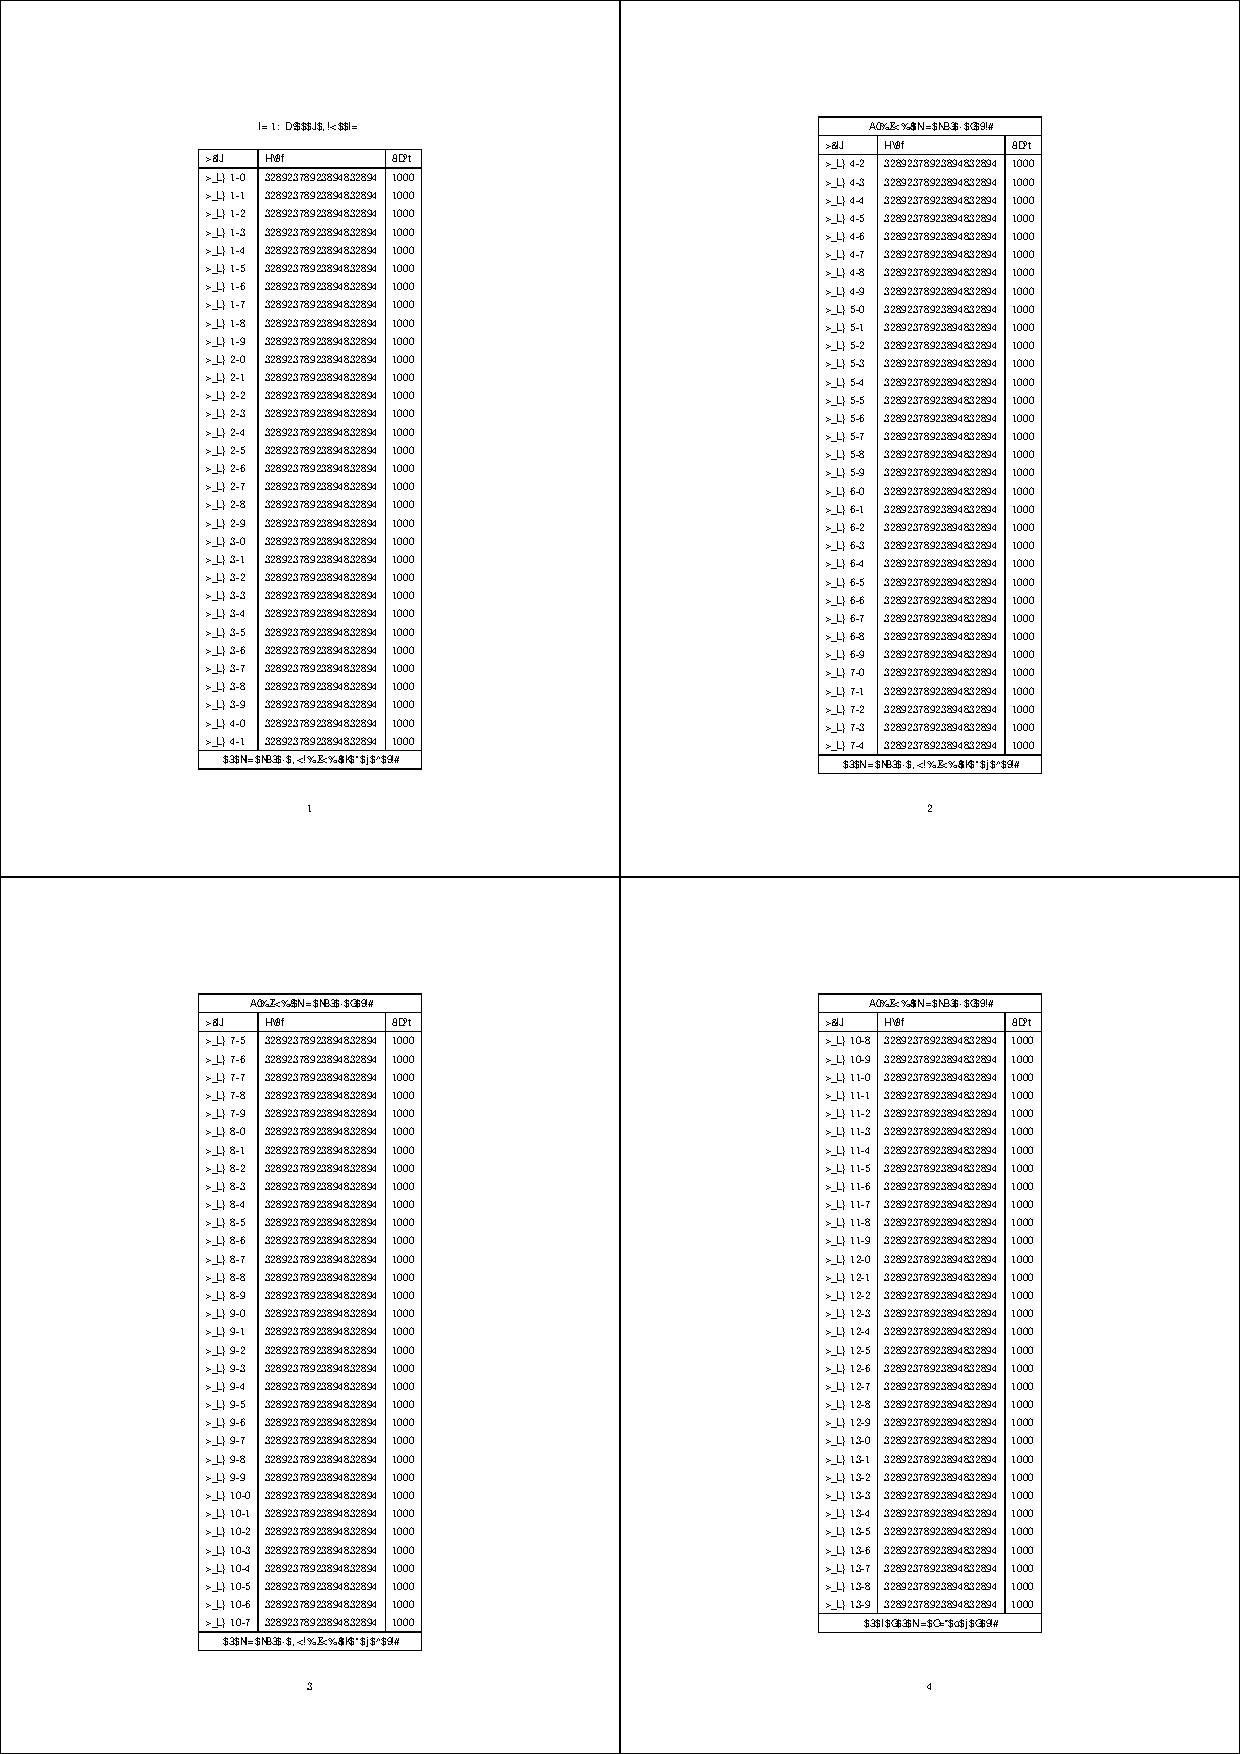
\includegraphics[width=\fullwidth]{images/longtable}%
   \IOlabel
   }%
   \caption{\Y{longtable}�λ�����ν��Ϸ��}\figlab{longtable}%
\end{figure}

%\end{comment} 

\subsection{ɽ�����λ���\zdash\Y{tabularx}}\seclab{tabularx}
\LaTeXe �� \E{array}/\E{tabular} �Ķ��Ǥ��������ľ�ܻ���Ǥ���
������ `\str p\pa{��}' ���Ѱդ���Ƥ��ޤ��������Ƥ�ɮ���Ƥ����ʳ�
�ǤϤ����������Ǥ��ʤ��������Ф��Ф���ޤ�����ưŪ�ˤ���������
�Ƥ����褦�ʴĶ�������������Ǥ��������� \Person{David}{Carlisle}�κ���
���� \Y{tabularx} �ѥå��������Ѥ������ \E{tabularx} �Ķ����Ȥ��ޤ���
\begin{Syntax}
\cmd{begin}\verb|{tabularx}|\pa{��}\pa{������}\\
\va{ɽ������������}\\
\cmd{end}\verb|{tabularx}| 
\end{Syntax}
�������ʲ��˼����ޤ���


\begin{InTeX}
\documentclass[a4j,10pt,papersize]{jsarticle}
\usepackage{tabularx}
\makeatletter
\def\hoge{\@tempcnta=\z@ \@whilenum \@tempcnta<10\do{%
   ��������\advance\@tempcnta\@ne}��}
\makeatother
\begin{document}
\hoge%
 \begin{center}
  \begin{tabularx}{\linewidth}{|X|X|X|}
   \hline
   \hoge & \hoge & \hoge \\
   \hline
  \end{tabularx}
 \end{center}
\hoge%
\begin{center}
 \begin{tabularx}{\linewidth}{|r|l|X|l|X|}
  \hline
  ����   & ���� & ����  & ���� & ��­���� \\
  \hline
  ��     &  500 & \hoge & 59A  & \hoge    \\
  \hline
  �䤫�� &  300 & \hoge & 9JA  & \hoge    \\
  \hline
 \end{tabularx}
\end{center}
\hoge%
\end{document}
\end{InTeX}

�嵭�����Ϥν������\figref{tabularx}�Ȥʤ�ޤ���

\begin{figure}[htbp]
 \begin{center}
\makeatletter
\def\hoge{\@tempcnta=\z@ \@whilenum \@tempcnta<10\do{%
   ��������\advance\@tempcnta\@ne}��}%
\makeatother
  \begin{tabularx}{\linewidth}{|X|X|X|}
   \hline
   \hoge & \hoge & \hoge \\
   \hline
  \end{tabularx}\par\vskip1em
 \begin{tabularx}{\linewidth}{|r|l|X|l|X|}
  \hline
  ����   & ���� & ����  & ���� & ��­���� \\
  \hline
  ��     &  500 & \hoge & 59A  & \hoge    \\
  \hline
  �䤫�� &  300 & \hoge & 9JA  & \hoge    \\
  \hline
 \end{tabularx}
\caption{\Y{tabularx}������ν��Ϸ��\label{fig:tabularx}}
\end{center}
\end{figure}
%
\E{tabularx} �Ķ��ˤ����������� `X' �������˻Ȥ���褦�ˤʤäƤ��ޤ���
\E{tabularx} �Ķ����Ȥ�٤�ɽ�������Τ�ɬ�פ�����ޤ���`X' ��ʣ���ξ���
���줾���������϶�����Ĺ���ˤʤ�ޤ���

\subsection{ɽ�����ٱ�ġ���}

{\LaTeX}�ǥ�������ɽ���Ȥ�ΤϽ鿴�Ԥˤ�
�ɤ����⤷��ޤ���GUI�١�����
�ץ�������ɽ��������������{\LaTeX}��
\env{tabular}�Ķ��ε��Ҥ��Ѵ�����ġ����
�Ȥ����ɤ��Ǥ��礦��Microsoft��\Prog{Excel}
��ȤäƤ������\Hito{����}{��Ϻ}��
\Prog{Excel2tabular}\footnote\webEtoT
�ʤɤ�����ޤ��Τǻ��ͤˤ��Ƥ���������������
�ץ�������{Microsoft}��\Prog{Excel}�Ǻ�����
�줿ɽ��{\LaTeX}�Υ��������Ѵ����ޤ���

Microsoft��Excel�ǤϤʤ�{OpenOffice.org}��
\Prog{Calc}��ȤäƤ���ʤ��\Hito{����}{��ʿ}��
\Prog[calc2latex]{Calc2\LaTeX}\footnote \webCtoL
�Ȥ�����Τ⤢��ޤ���
�����Ȥ���Calc�Ǻ�������ɽ��\env{tabular}�Ķ���
�Ѵ�����ɽ�Ȥ���{\LaTeX}��Ž���դ�������Ǥ��ޤ���

�Ƕ�Ǥ�ľ�� \LaTeX ���� \Prog{Excel} �ե�������ɤ߹����
\Person{Hans-Peter}{Doerr}�ˤ�� \Y{exceltex} �ѥå�������
����ޤ�\footnote{\webExceltex}��
\Prog{Perl}������ץȤ���𤹤���ǻ��ꤷ������䥷���Ȥ��ɤ߹��������
���ޤ���

% end of table


\section{�ޤ˴ؤ�������Ȳ����ΰ���}\label{sec:figure}

�ޤ������˴ؤ��Ƥ��礭��ʬ����2�̤����ˡ������ޤ�����Ĥϥڥ���ȥ�
�եȤʤɤǽ񤤤������򤽤Τޤ޼�������ˡ�� �⤦��Ĥ�{\LaTeX}��
\env{picture}�Ķ��ǿޤ�ľ�ܽ���ˡ�Ǥ���

\LaTeX �ˤ�\Env{picture}�Ķ��ȸƤФ���ñ��\Z{���}�򤹤뤿���
����Ķ����Ѱդ���Ƥ��ޤ�������\Env{picture}�Ķ����ĥ����
\Y{epic}, \Y{eepic}, \Y{pict2e}�ʤɤ�¸�ߤ����������٤κ�ޤ�
�Ǥ��륳�ޥ�ɤ��Ѱդ���Ƥ��ޤ���\Env{picture}�Ķ��Ȥ��μ��դξܤ���
����\wasyo{\COMP}\cite{latexcomp}��\wasyo{\GCOMP}\cite{graphicscomp}
�򻲾Ȥ��Ƥ���������

���餫�γ����ץ������Ǻ������� BMP, JPEG, PNG, EPS, PDF ���β�����
\LaTeX ��ĥ����ि��ˤϡ�����Ū�ˤ�\sty{graphicx}�ѥå��������Ѥ��ޤ���

\LaTeX ���ȤǤϲ����ե������ľ��Ū�˰������Ȥߤ��Ѱդ���Ƥ��餺��
�����ե�����˴ؤ���¿���ν�����ǥХ����ɥ饤�ФȤ��������ץ������˰�
¸���������뤿�ᡤ��ʬ�λȤ����Ȥ��Ƥ���ǥХ����ɥ饤�Ф��ɤΤ褦�ʲ�
���������б����Ƥ���Τ����ΤäƤ����������ǽ�Ū�˽��Ϥ�����ʸ�������
PDF�ʤ��\prog{\Dvipdfmx}��\PS �ʤ��\prog{dvips}��Ȥ����ˤʤ�ޤ���
��ǯ�Ǥ�DVI ��������ľ�� PDF �������Ǥ���\Dvipdfmx ��Ȥ����򶯤��侩��
�ޤ���\Dvipdfmx ���Ѥ������BMP, JPEG, PNG, \Z{EPDF}��ñ��ڡ�����PDF��, 
EPS ������ĥ����ߤ���ǽ�Ȥʤꡤ����� DVI �ե����뤫��ľ�� PDF ��������
������Ǥ��ޤ���

�Ƕ��ư���Ȥ�����ʸ������С������ˤ� PDF ���Ѥ����礬�����Ƥ���
�褦�Ǥ���\Dvipdfmx ��Ȥ��� \LaTeX �Ǥ��Τޤ� PDF ������������
���⥵�ݡ��Ȥ��Ƥ��뤿�ᡤ����ϲ�����������꤬�ʤ��¤ꡤ\Dvipdfmx 
��Ȥ��褦�ˤ���Ȳ������������Ȼפ��ޤ���
\zindind{����}{��ĥ�����}%

��ǯ�ޤ�{\LaTeX}�Ǥ�EPS�ʳ��β�����ĥ����ߤ��񤷤��Ȥ����Ի�����Ū����
�⤬����ޤ����������ߤ� \Dvipdfmx ���о�ˤ������ϴ�ʬ�Ѳ����Ƥ��ޤ�
�������줫����Ѳ�����ȹͤ����ޤ���



\section{�����ե������ĥ�����}\seclab{gazou}

\LaTeX\ �Ǥϥӥåȥޥåײ����䡤����������ʤɤ�¿���ν�����ǥХ����ɥ�
���ФȸƤФ�볰���Υץ������˰�¸���Ƥ��ޤ������Τ��ᡤ\LaTeX\ �Dz���
�ե�����򰷤����ϡ��ޤ��ǥХ����ɥ饤�Ф������̤����򤹤���ˤʤ��
����


\subsection{�ǥХ����ɥ饤�Ф�����}

�Ƽ�ΥǥХ����ɥ饤�Хץ������ˤ���������������Ф����б�������
\tabref{ddimage}�˼����ޤ���\genzai �Ǥ��б������ˡ�
\begin{table}[htbp]
 \begin{center}
  \caption{�Ƽ�ǥХ����ɥ饤�Фβ��������б�����}\tablab{ddimage}
  \begin{tabular}{ll}
  \TR
  \Th{�ǥХ����ɥ饤��} & \multicolumn{1}{c}{\Th{�б���������}}\\
  \MR
  xdvi      & EPS*  \\
  dvips     & EPS   \\
  \Dvipdfmx & EPS*, EPDF, PNG, BMP, JPEG\\
  \Dviout    & EPS*, \Prog{Susie} {plug-in} �ˤ��¾�η������б���ǽ\\
  \BR
  \end{tabular}
 \end{center}
\end{table}
�������Ĥ��Ƥ����Τ�\GS �ʤɤγ����ץ�������ɬ�פȤ�������Ǥ���

{\LaTeX}�Dz�����ĥ��������¿���ξ���ɸ��Ū��\sty{graphicx}�ѥå�������
�Ȥ����ˤʤ�ޤ���\Dvipdfmx ��ȤäƤ�����ϥѥå��������ץ����
��\Option{dvipdfmx}�Ȥ��ޤ���

\begin{InText}
\usepackage[dvipdfmx]{graphicx}
\end{InText}

����ˤ��\sty{graphicx}�ѥå�������\fl{dvipdfmx.def}�Ȥ�������ե������
�ɤ߹��ߤޤ����⤷�� \Fl{dvipdfmx.def}�Ȥ����ե����뤬¸�ߤ��ʤ��褦�Ǥ�
��С��ʲ���URL����ե�����������`\str{$texmf/tex/latex/graphics/}'��
�Υǥ��쥯�ȥ�˥��ԡ����Ƥ�������%
\footnote{\url{http://tex.dante.jp/jou1/dvipdfmx.def}}��


�Ť� \TeX/\LaTeX ��2006ǯ�����ˤ����󥹥ȡ��뤵��Ƥ���ΤǤ���С�
\option{dvipdfmx}�ǤϤʤ���\Option{dvipdfm}���ץ�������ꤷ�ơ�
\Dvipdfmx �� PDF ��ǥХ����ɥ饤�ФȤ��ޤ�\footnote{���������
��ͳ���ʤ��¤� \TeX �Ķ������Ū�˹����������˾�ޤ����Ǥ���}��

\begin{InText}
 \usepackage[dvipdfm]{graphicx}
\end{InText}

Unix��OS�ʤ��{\PS}�Τۤ����ɤ��Ǥ��礦����\Option{dvips}��\sty{graphicx}
�ѥå������Υ��ץ����Ȥ��ޤ���\prog{dvipsk}�Ǥ�������\prog{pdvips}����
����\Option{dvips}���ץ�����Ȥ��ޤ���

¾�ˤ�\prog{xdvi}�䡤Windows �Ǥ���� \Dviout �����Ǥ��ޤ���
Windows�����Ǽ�����β����ΤۤȤ�ɤ��ӥåȥޥåפ�¸�ߤ���ʤ��\Dviout
��ǥХ����ɥ饤�Ф����򤹤���ɤ��Ǥ��礦��\Dviout �Ǥϥץ�ӥ塼�������
�Ԥ��ޤ���
\Dviout �ξ���\Dviout �����󥹥ȡ��뤵��Ƥ���ե������
\fl{GRAPHIC/LATEX2E/dviout.def}�Ȥ����ե�����
�� \fl{\$texmf/tex/latex/graphics/} �˥��ԡ����Ƥ�������\footnote{\Dviout ��
���EPS�����������Ȥ���\prog{\GS}�ˤ�EPS��\Z{PPM}���Ѵ����Ƥ������
��ɽ�����ޤ�����\prog{\Dviout}��\prog{Ghostscript}�˴ؤ��������Ŭ�ڤ˹Ԥ�
�Ƥ���������}��

EPS������¿���ʤ�Ф�����ˤ��Ƥ�1��EPS����PDF���Ѵ����Ƥ���
\prog{\Dvipdfmx}��Ȥ��Τ��ɤ��Ȼפ��ޤ���%\unixos �ʤ�м�����β�����
%EPS���Ѵ�����\prog{dvips}��Ȥ����Ȥˤʤ�Ǥ��礦��


\subsection{����Ū�ʼ��}

�����ե������\LaTeX ��ʸ���ĥ�����ˤϡ�����Ū�˼��Τ褦�ʼ���Ƨ��
���ˤʤ�ޤ���

\begin{enumerate}
\zindind{�ե����}{�Υ����ȥ饤��}%
\zindind{PDF}{������ĥ�����}%
\item �����ץ�������PDF��EPS�����ǥե��������¸����¸�������
      ���ץ����Dz�ǽ�Ǥ���Хե���Ȥϥ����ȥ饤�󲽤������顼��
      ��¸���ʤ��褦�ʥե�����Ȥ��ޤ���
\item ʸ��Υץꥢ��֥��\sty{graphicx}�ѥå�������Ȥ�����������ޤ���
\item \sty{graphicx}�ѥå������ˤ�\K{�ǥХ����ɥ饤��}����ꤷ�ޤ���
      \PS ������ʸ�����Ϥ���ʤ�С�\Option{dvips}����ꤷ�ޤ���PDF�������
      �����Ȥ���\prog{\Dvipdfmx}��Ȥ������\Option{dvipdfmx}����ꤷ�ޤ���
\item EPS�ʳ��β����Ǥ����\LaTeX �����Ǥ������\K{�Х���ǥ��󥰥ܥ�
      ����}����ꤷ�ޤ���
\item  �ޤ��������٤����� \C{includegraphics}̿���Ȥäƥե�����̾��
      �����ޤ���
\end{enumerate}

�ǥХ����ɥ饤�Ф�\Dvipdfmx ���ϲ����ե�����򰷤�������ǽ�Ǥ�����\LaTeX
�ϲ����ե������ľ�ܰ��������Ǥ����������˴ؤ�����������Ǥ��ޤ���
���Τ��ᡤ\Dvipdfmx �ˤ�����\Z{JPEG}��\Z{PNG}��\Z{PDF}, \Z{BMP}�β�
���ե������\KY{�Х���ǥ��󥰥ܥå���}�Ȥ��������Ρ�\Z{������ɸ}��ޤ��
\zindind{����}{�θ�����ɸ}%
�����������Ϳ�������ĥ����������ǽ�Ǥ�������Ū�ˤϲ����β���Ĺ���Ƚ�
��Ĺ���Υ���������ꤹ����Ȥʤ�ޤ����Х���ǥ��󥰥ܥå�����
\Va{filename}{img}�Ȥ��������ե����뤬����С�\Va{filename}{bb}�Ȥ���
�ե������\sty{graphicx}�ѥå����������Ȥ���褦�ˤʤäƤ��ޤ���

\Dvipdfm ����°����\Prog{ebb}�Ȥ����ץ������Dz����ΥХ���ǥ��󥰥ܥ�
��������Υե����� \Va{filenam}{bb}������Ǥ��ޤ����б����Ƥ����������
��JPEG, PNG, PDF �Ǥ�\footnote{ebb�ʳ��ˤ�\Prog{identify}���ޥ�ɤ�\Prog{file}��%
�ޥ�ɤǥ�����������Τ�����Ǥ��ޤ�����Windows��Mac~OS~X�Ǥ����%
\Prog{�������ץ�����}��\Prog{�ե��������}�ˤ�ɽ������ޤ���}��

JPEG��PNG��PDF��EPS��ľ��PDF��ĥ�����ޤ�������Ū�ʼ��Ȥ���
�ϡ��ե������¸�ߤ���ǥ��쥯�ȥ��
\begin{InTerm}
\type{ebb filename.jpg}
\end{InTerm}
�Ȥ���г�ĥ�Ҥ�\exten{bb}��\Va{filename}{bb}�Ȥ����ե����뤬
��������ޤ����������줿\Va{filename}{bb}�򸫤Ƥߤޤ���

\begin{InText}
%%Title: ./filename.jpg
%%Creator: ebb Version 0.5.2
%%BoundingBox: 0 0 595 842
%%CreationDate: Tue Dec 30 13:04:10 2003
\end{InText}

�嵭�Τ褦��\va{�ե�����̾}��\va{�����ץ������}�� \va{�Х���ǥ��󥰥ܥ�
����}�� \va{��������}�ξ��󤬽��Ϥ���ޤ�������\Va{filename}{bb}�Υե���
�����¸���Ƥ����Τ����ޤ����ʤ����ϡ�������������ե�������ɤ߹����
����ս�ǡ����Τ褦�ˤ����\Va{filename}{bb}���ʤ��Ƥ��ɤ����ˤʤ��
����

\begin{InText}
\includegraphics[bb={0 0 595 842}]{filename.jpg}
\end{InText}

���Ѥ�������Υե�����̾��\Va{�ե�����̾}{��ĥ��}��
\qu{\fl{filename.png}}�Τ褦��\Va{8ʸ��}{3ʸ��}�Ȥ����ۤ����ߴ����ξ�ǰ�
���Ǥ���


\begin{Exe}
���˥ե�����̾��\fl{image.png}�β��������ä��Ȥ���С����󥽡��뤫��
\type{ebb image.png}�Ȥ���\fl{image.png}�Ѥ�\fl{image.bb}������������
���ǧ���Ƥ�������������\texttt{image.bb}�ϲ����ե�����νIJ�����������
������Υե�����Ǥ���\texttt{image.bb} �򸫤��ʬ����ޤ�������Ȥϼ�
�Τ褦�ʤ�ΤˤʤäƤ���Ȼפ��ޤ���

\begin{InText}
%%Title: ./image.png
%%Creator: ebb Version 0.5.2
%%BoundingBox: 0 0 595 841
\end{InText}

\qu{\str{BoundingBox}}�Ȥϸ�����ɸ�Ȳ����νIJ���Ĺ�����ͤǤ������˥�����
�ե������ʲ��Τ褦�ˤ��ޤ���

\begin{InText}
\documentclass[papersize]{jsarticle}
\usepackage[dvipdfmx]{graphicx}
\begin{document}
\centering \includegraphics[width=4cm]{image.png}
\end{document}
\end{InText}

��Ϥ��Ĥ��̤�˥����ץ��åȤ���DVI�ե������������\prog{\Dvipdfmx}��PDF
��������ޤ�������ˤ�� \fl{image.png}��ĥ����ޤ줿 PDF ������������
���Ǥ���
\end{Exe}

\subsection{ĥ����ߤˤ����륪�ץ����}

�����ץ������Ǻ������ơ����Ǥ�¸�ߤ���褦�ʲ����� \C{includegraphics}
̿���ĥ����ߤޤ���
\begin{Syntax}
\C{includegraphics}\opa{����}\pa{�ե�����̾}
\end{Syntax}

\va{����}�˴ؤ��Ƥϰʲ��˼����褦�ʥ��ץ���󤬻��ѤǤ��ޤ���

\begin{description}
\zindind{����}{�ι⤵}%
 \item[\str{height=}\va{�⤵}]
    ñ���դ��Dz����ι⤵����ꤷ�ޤ���
 \item[\str{totalheight=}\va{����Ū�ʹ⤵}]
    ñ���դ��Dz���������Ū�ʹ⤵����ꤷ�ޤ���
\zindind{����}{����}%
 \item[\str{width=}\va{��}]\indindz{��}{������}%
    ñ���դ��Dz�����������ꤷ�ޤ��� 
 \item[\str{scale=}\va{����}]
\zindind{����}{���}%
    �����γ���Ψ����ꤷ�ޤ��� \indindz{����}{�ޤ�}
 \item[\str{angle=}\va{����}]
\zindind{����}{�β�ž}%
    \K{ȿ���ײ���}�������ž������٤���ꤷ�ޤ��� 
 \item[\str{origin=}\va{����}]
    �����δ��������ޤ��� 
 \item[\str{bb=}\va{����}]
    \KY{�Х���ǥ��󥰥ܥå���}�ȸƤФ��������礭���ȸ�����ɸ����ꤷ�ޤ���
    �����Τɤ��ΰ��Ȥ��٤�������ꤷ�ޤ���\zindind{����}{�ΥХ���ǥ��󥰥ܥå���}%
    \qu{\str{bb=0 0 640 480}}�Ȥ���ȸ�����
    \xy{0}{0}�Ȥ��ƽIJ�\qu{$640\times480$}
    ���ΰ��Ȥ��褦�ˤ��ޤ���
 \item[\str{viewport=}\va{����}] 
\zindind{����}{���ڤ�ȴ��}%
	    �����������ΰ����ꤷ�ޤ����ڤ�ȴ���Ǥ���
%	    \str{viewport={30 30 600 40}}
 \item[\str{trim=}\va{����}] 
\zindind{����}{�Υȥ�ߥ�}%
	    ������ü���ڤ�ȴ���ޤ���
%	    \str{trim={3 3 2 2}}
 \item[\str{noclip}] 
  �����Ѥ˻Ȥ��٤��ΰ�򸵤β������Ϥ߽Ф��Ƥ���
  ���˲������ڤ�ȴ���ʤ��褦�ˤ��ޤ���
 \item[\str{clip}] 
\zindind{����}{�Υ���åԥ�}%
  ���������ݤ��줿�ΰ�����礭������
  �ڤ�ȴ�����ޤ���
 \item[\str{draft}] 
 �ºݤ˲�����ĥ����ޤ��˲�������ͭ��
 ��������ΰ褬�Ȥˤ������ɽ���ˤʤꡤ�ե�����̾��ɽ�����ޤ���
 \item[\str{keepaspectratio}] 
\zindind{����}{�νIJ���}%
 ����̾������Ȥ��˽IJ������¸����褦�ˤ��ޤ���
 \sty{graphicx}�ѥå�������ɸ��Ǥ���¸����ޤ���
\end{description}

\begin{Exe}
����ʬ�λ��äƤ������\va{�ե�����}��\va{�ǥХ���}��
�������Τ����Ƥߤ��������ʹ�Ƭ�Υѡ�����Ȥϼ�������
\fl{images}�ե������\Fl{gnu-head.pdf}��\fl{gnu-head.bb}������Ȳ��ꤷ�ޤ��ˡ�
\begin{InOut}
\usepackage[dvipdfmx]{graphicx}
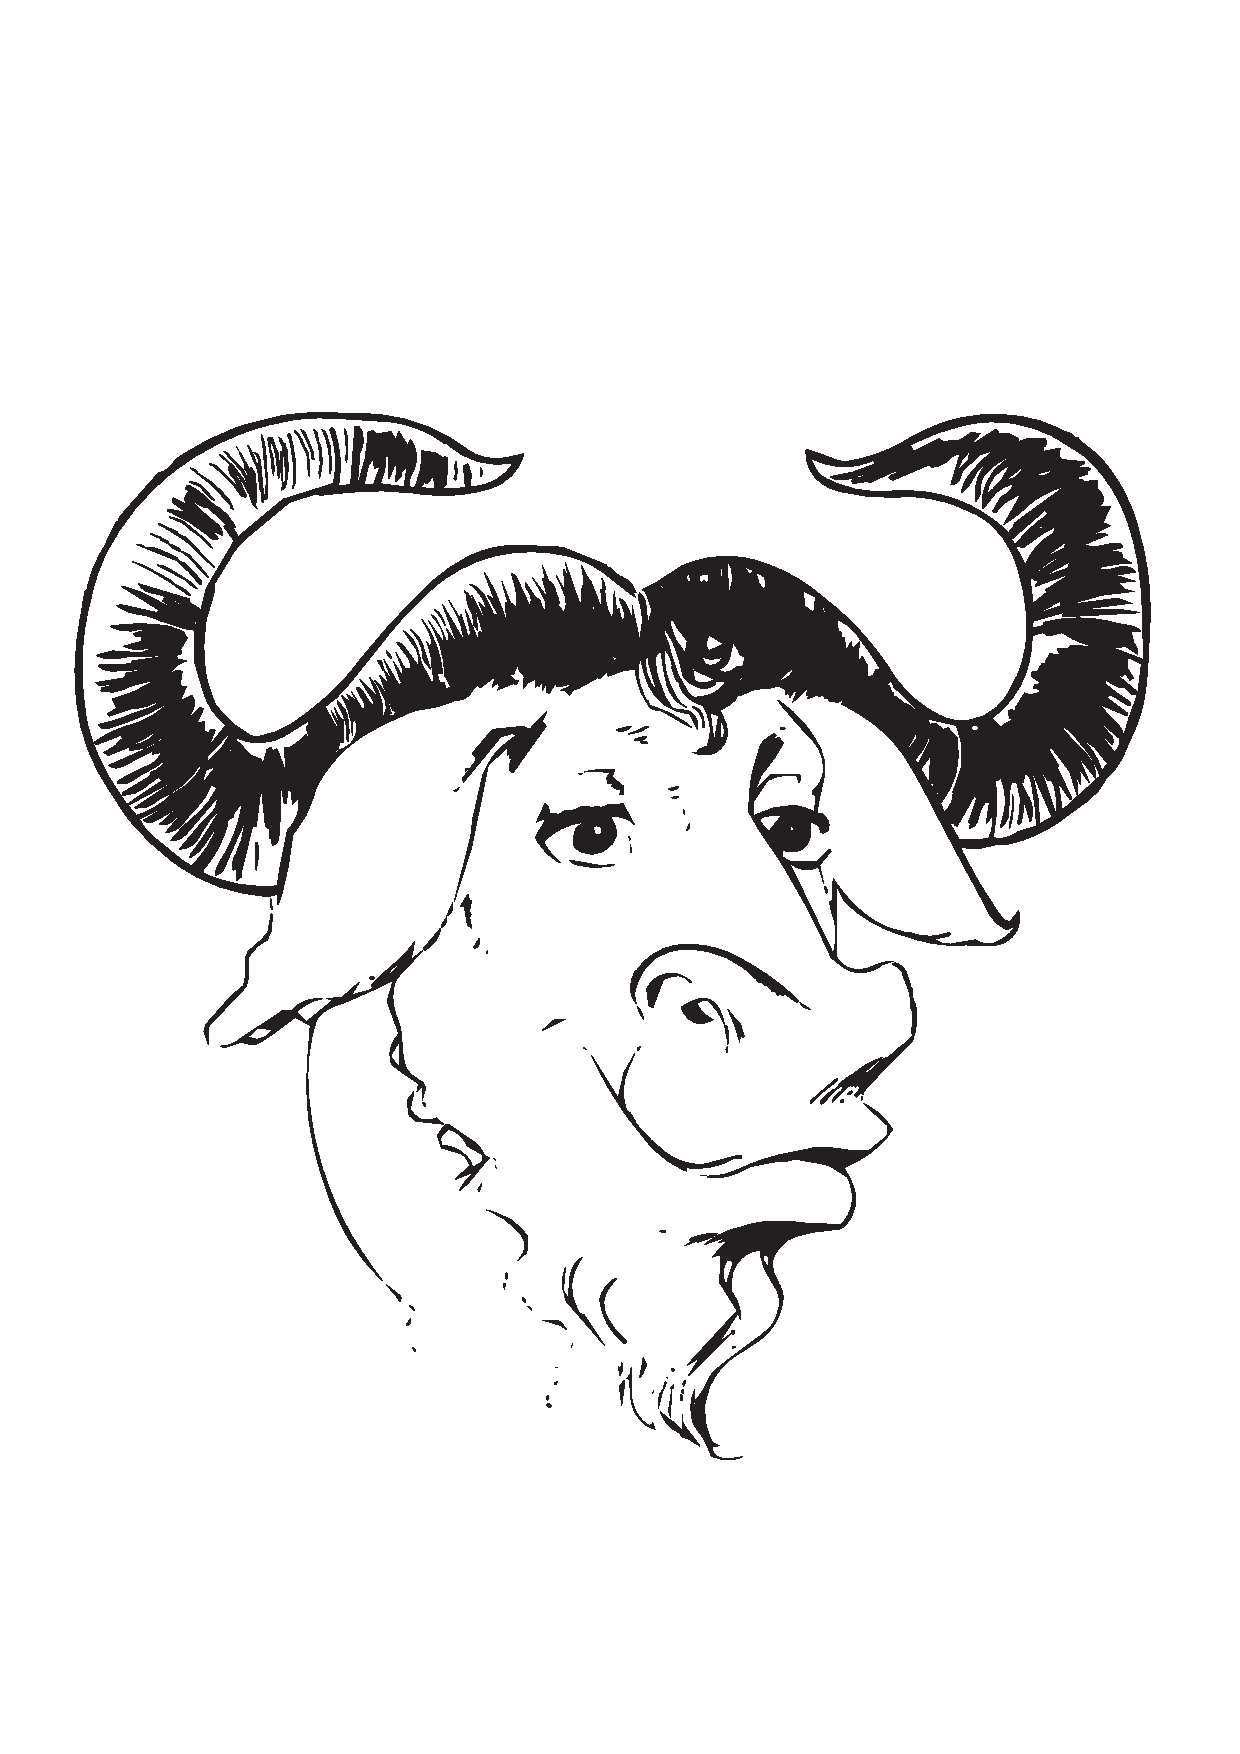
\includegraphics[width=3cm]
  {images/gnu-head}
\end{InOut} 
\end{Exe}

\begin{InOut}
\usepackage[dvipdfmx]{graphicx}
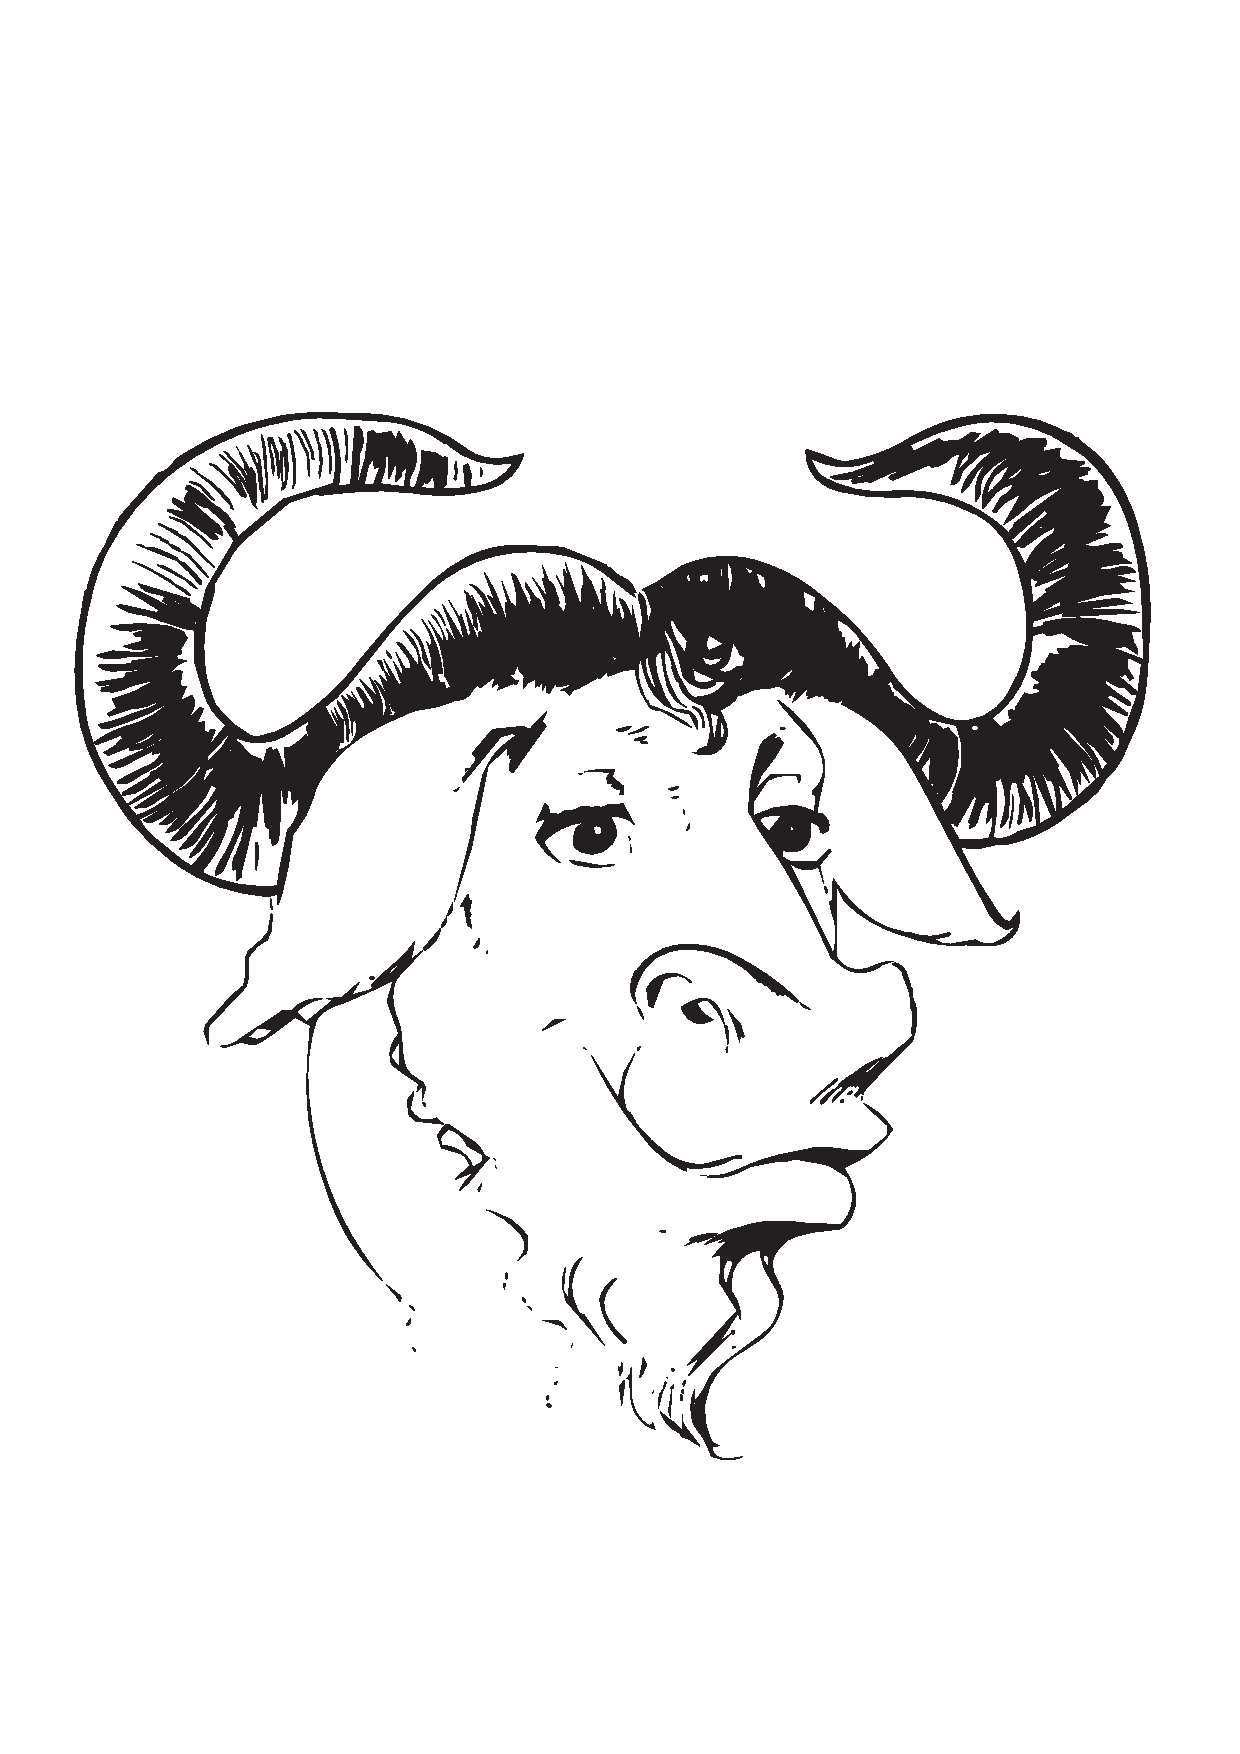
\includegraphics[width=2cm,
  trim=20 20 20 20]
  {images/gnu-head} 
\end{InOut}

\begin{InOut}
\usepackage[dvipdfmx]{graphicx}
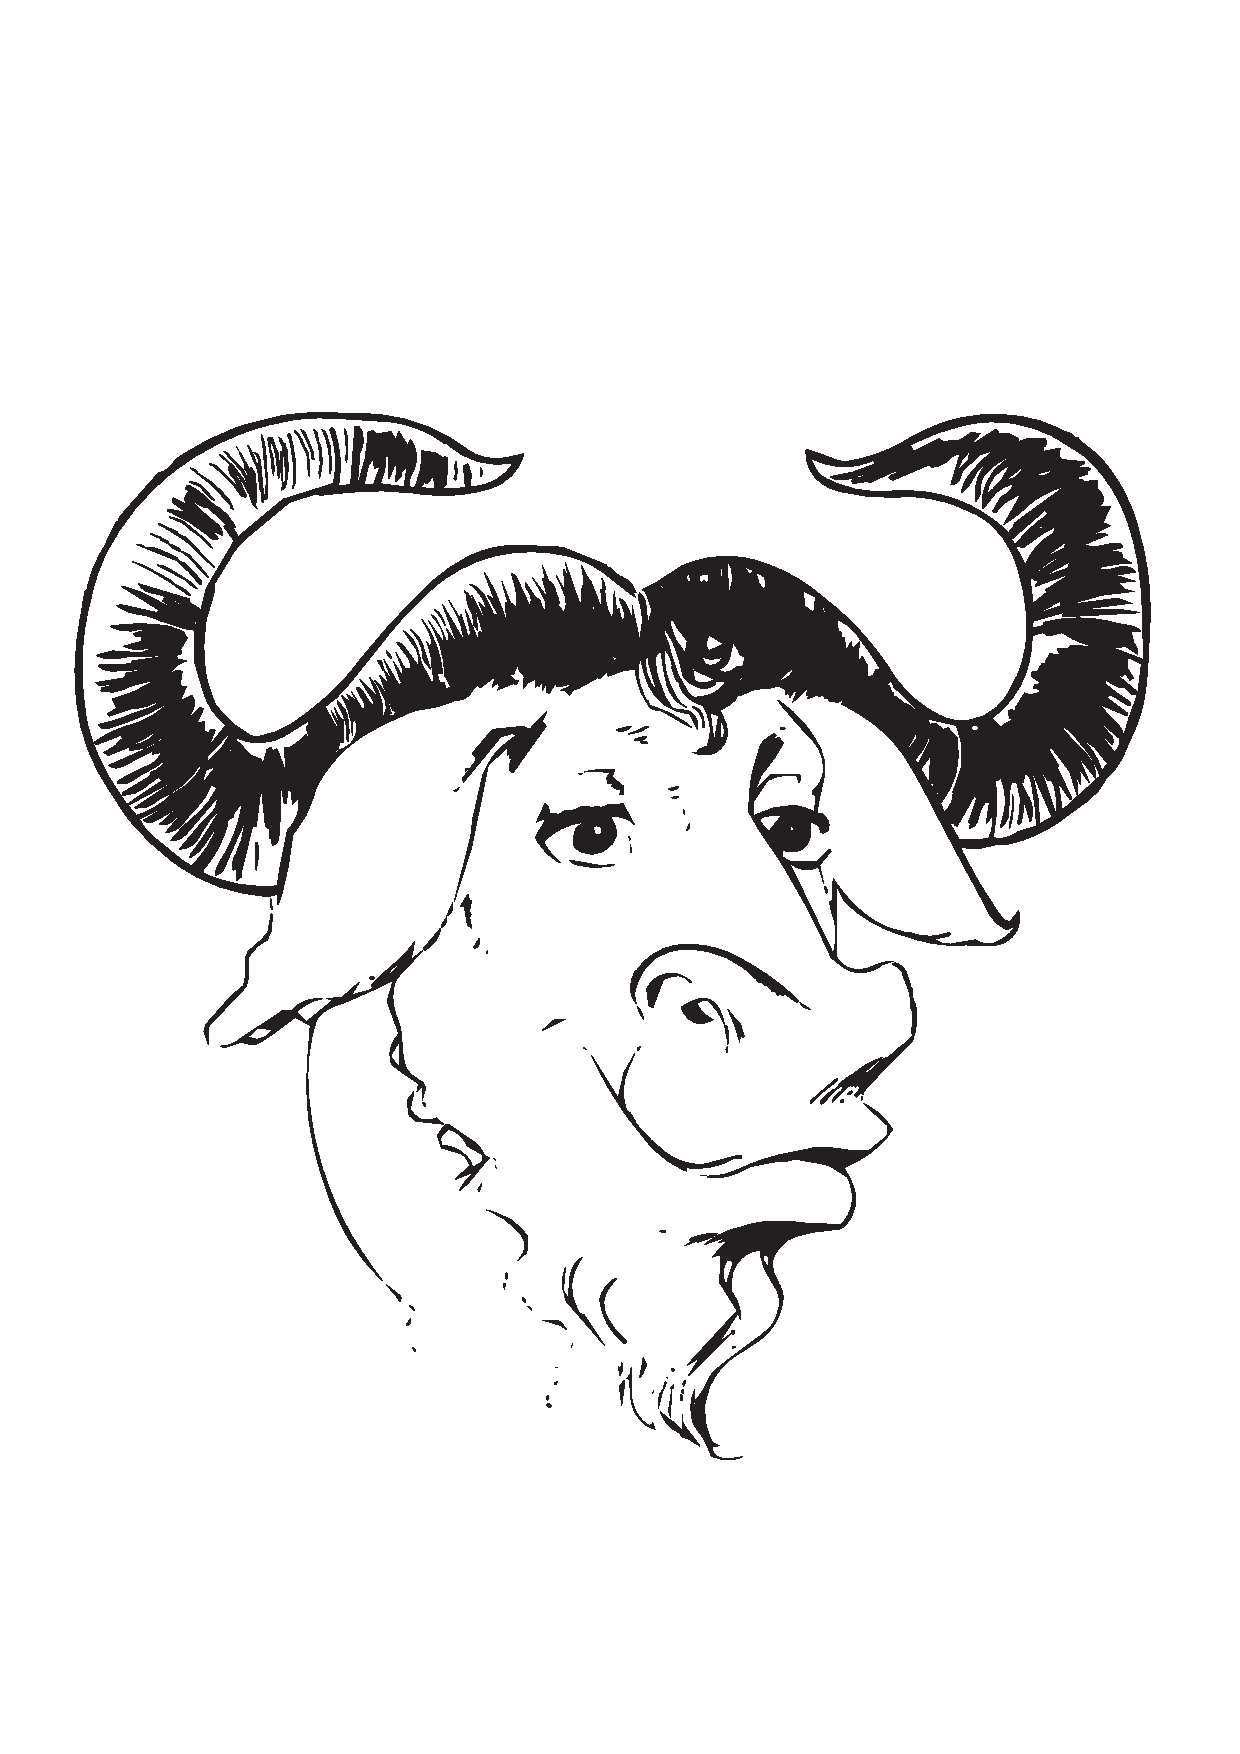
\includegraphics[width=2cm,
  clip,viewport=131 304 459 548]
  {images/gnu-head}  
\end{InOut}

\begin{InOut}
\usepackage[dvipdfmx]{graphicx}
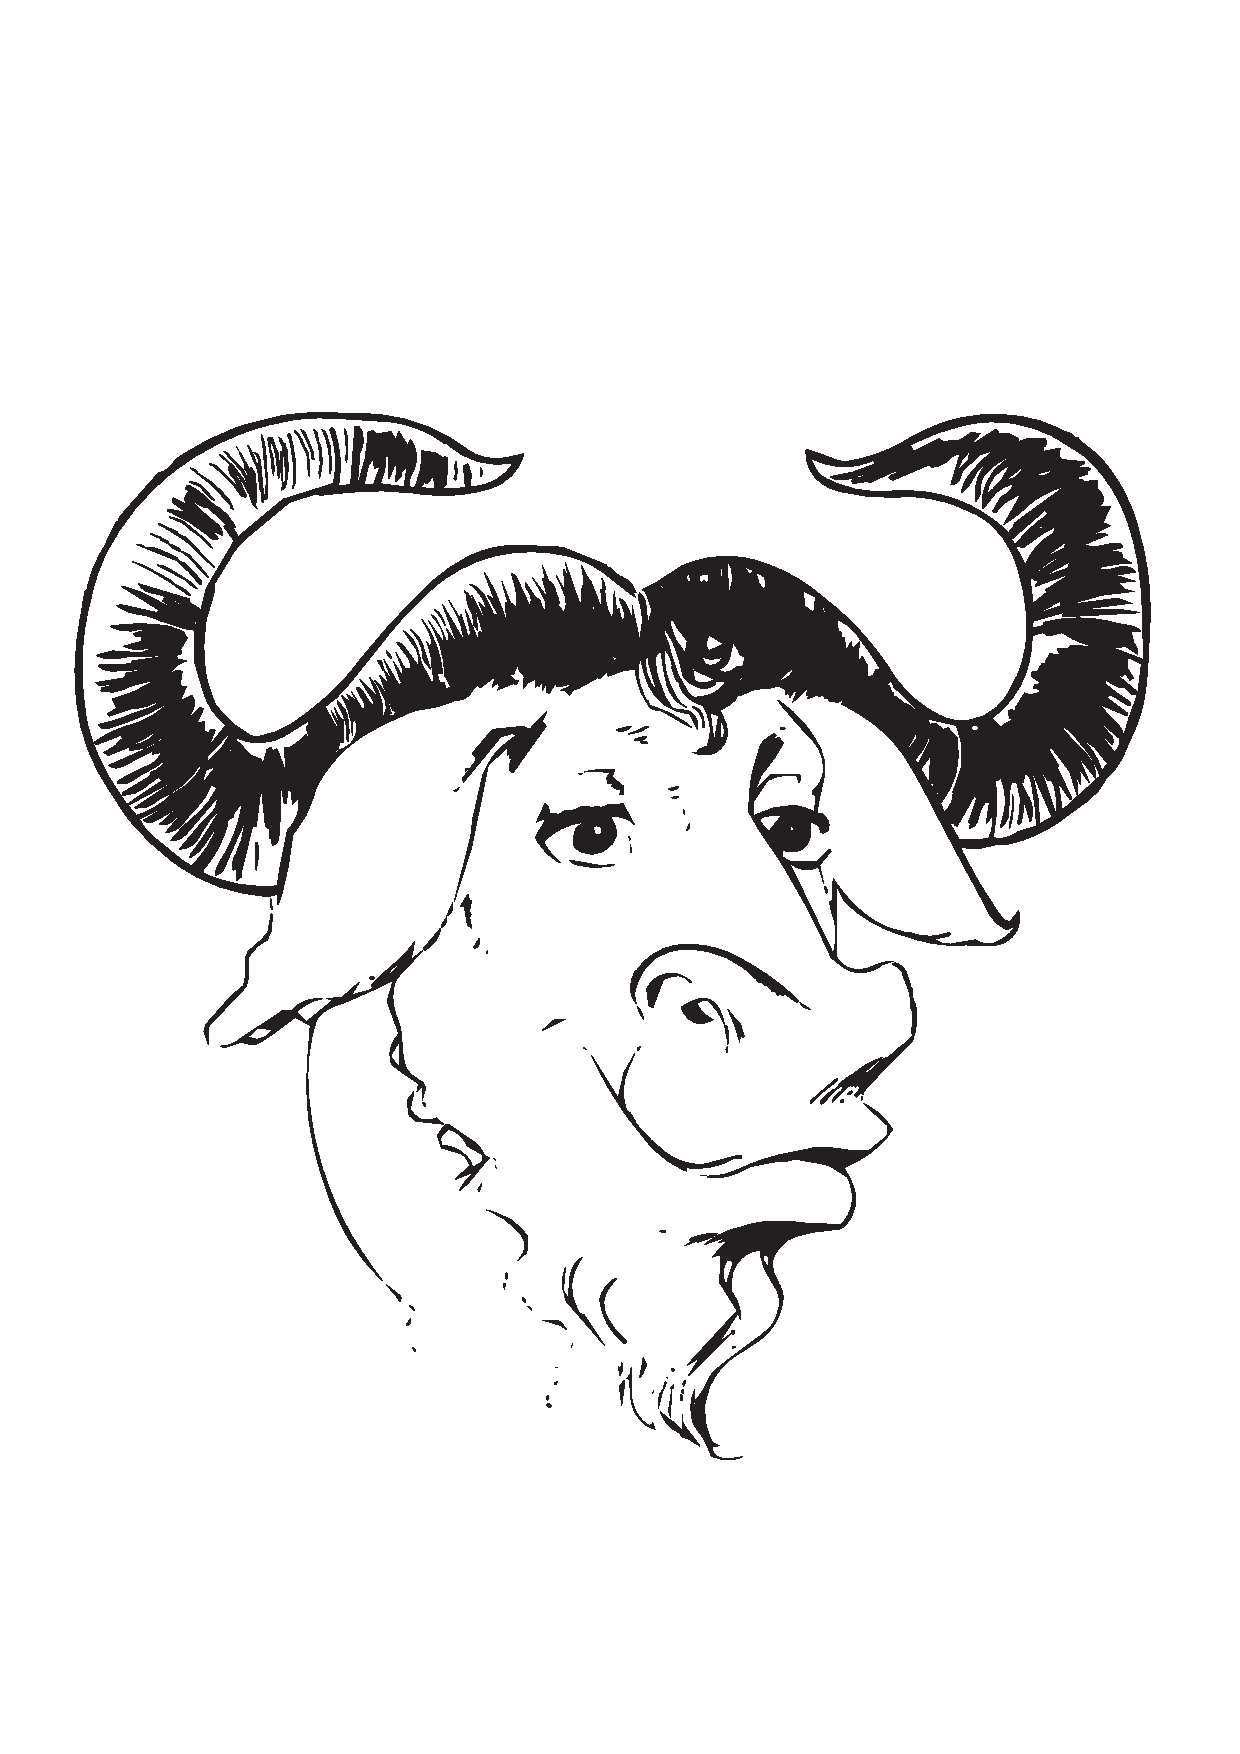
\includegraphics[width=2cm,angle=30,
  clip,viewport=131 304 459 548]
  {images/gnu-head}   
\end{InOut}

\begin{InOut}
\usepackage[dvipdfmx]{graphicx}
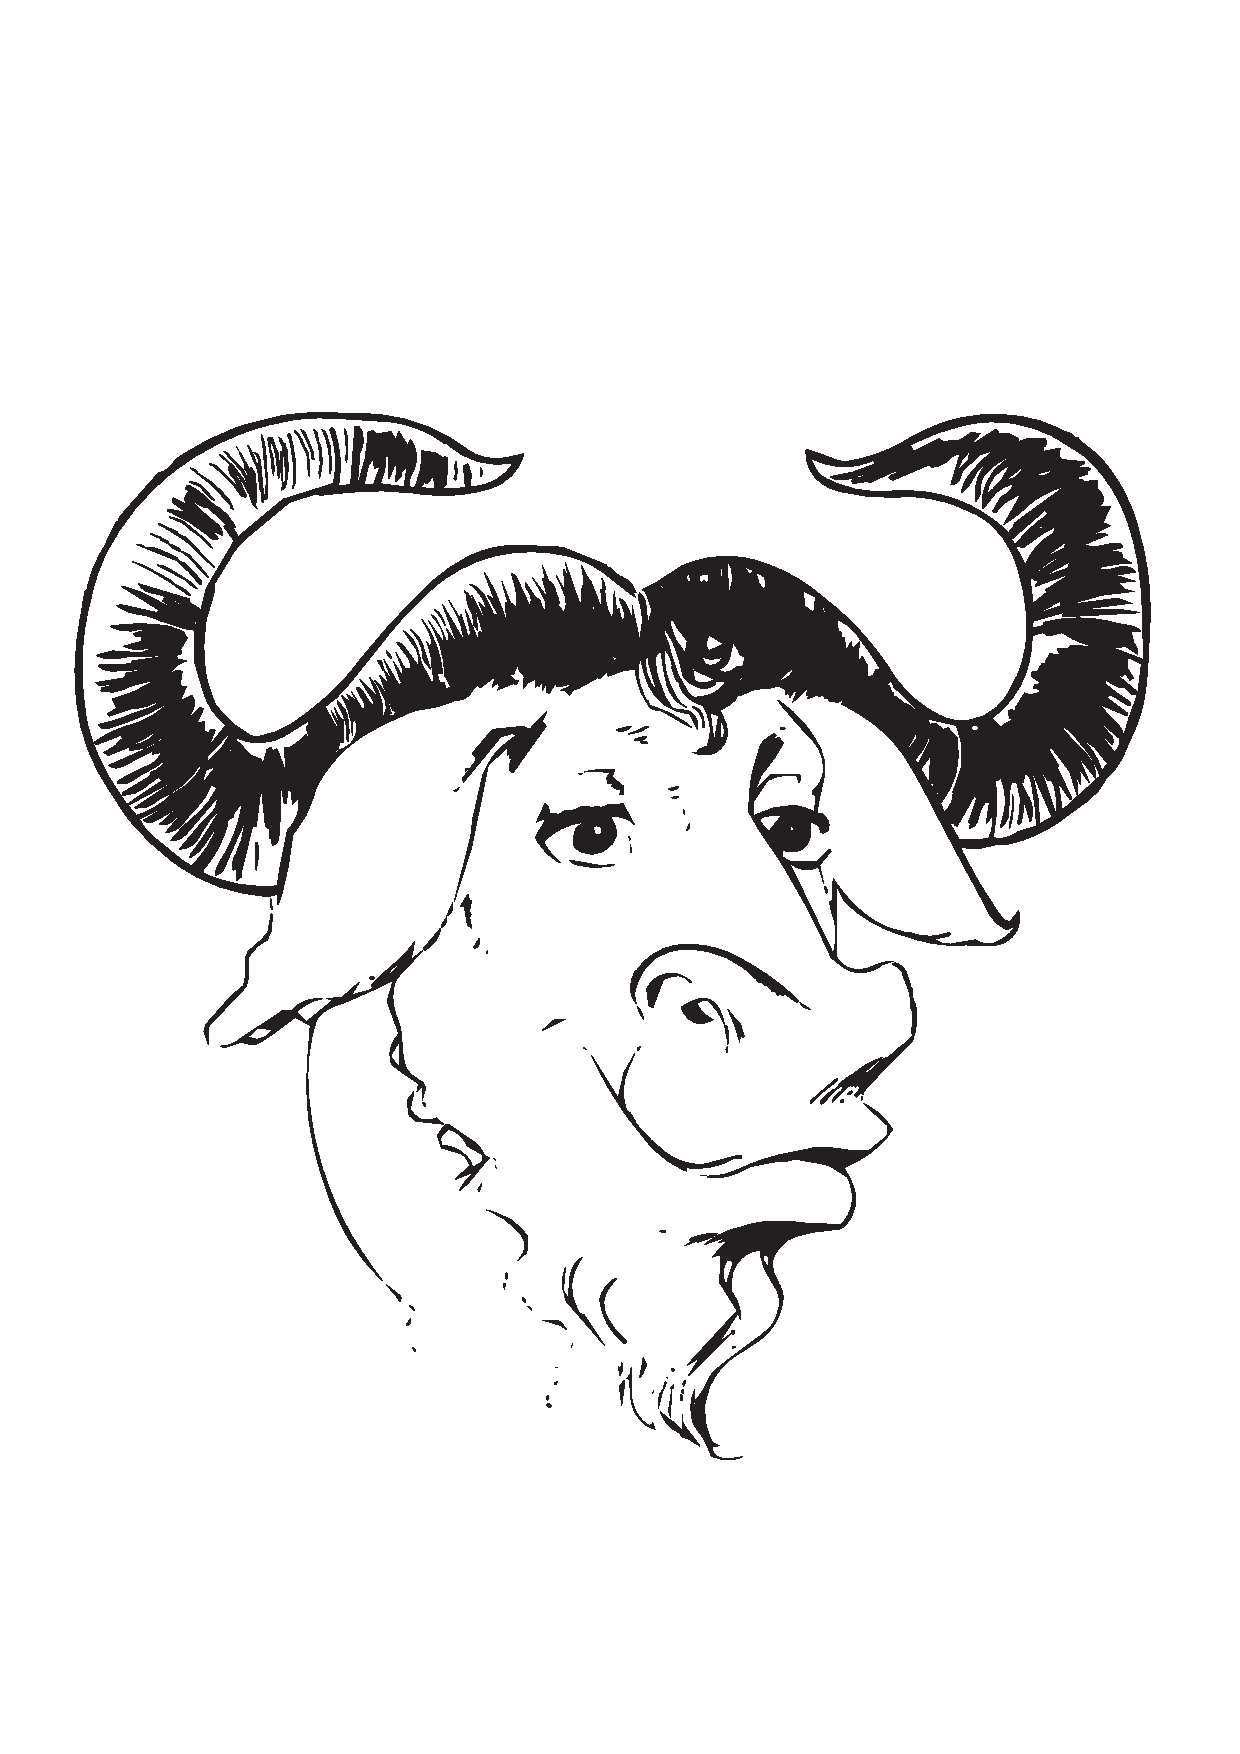
\includegraphics[width=2cm,angle=90,
  clip,viewport=131 304 459 548]
  {images/gnu-head}    
\end{InOut}

\subsection{�����γ�����ž�������}

�ޤʤɤ�ȿ���ײ���\kaku{90}��ž�������������Ǥ��礦��
���ξ��� \Cmd{rotatebox}̿���Ȥ��ޤ���
\begin{Syntax}
\Cmd{rotatebox}\opa{����}\pa{����}\pa{����}
\end{Syntax}
����� \cmd{includegraphics}��Ǥ�հ�����
\qu{\str{angle}}��Ȥä�����Ʊ���Ǥ���
 \cmd{rotatebox}�Ͽޤ˸¤餺���������ǡ�ɽ���ǽ�ˤ�
\Z{��ž}���ޤ���\va{����}�ι��ܤˤϰʲ��Τ褦��
��Τ�����ޤ���
\begin{description}
\item[\str{origin=}\va{��٥�}] 
 ���Ǥ��ž���뤿��θ�������ꤷ�ޤ���%%
 ��\qu{\str l}����\qu{\str r}�����\qu{\str c}��
 ����\qu{\str t}������\qu{\str b}������Ǥ��ޤ���
\item[\str{x=}\va{��}] 
$x$�����θ����ΰ��֤�ľ��\va{Ĺ��}����ꤷ�ޤ���
\item[\str{y=}\va{��}]
$y$�����θ����ΰ��֤�ľ��\va{Ĺ��}����ꤷ�ޤ���
\end{description}

\indindz{��ž}{ʸ�����}%%%
\begin{InOut}
\rotatebox{70}{ʸ����ʤ�}��
\rotatebox[origin=c]{60}{��ž�Ȥ�}��
\rotatebox[origin=b]{50}{�ɤ�}
\rotatebox{30}{�Ǥ���?}
\end{InOut}
%
���Ǥ�\K{����̾�}����ˤ� \cmd{scalebox}��
�Ȥ��ޤ���\index{����}\index{�̾�}\indindz{����}{ʸ�����}
\begin{Syntax}
\Cmd{scalebox}\pa{���γ���Ψ}\opa{�Ĥγ���Ψ}\pa{����}
\end{Syntax}
\va{����Ψ}�ˤ�Ĺ������ꤷ�ޤ���\begin{InOut}
\scalebox{2.3}{����̾�}\par
\scalebox{3}[1]{����̾�}
\end{InOut}

���Ǥ�\K{ȿž}�ˤ� \cmd{reflectbox}��Ȥ��ޤ���
\begin{Syntax}
\Cmd{reflectbox}\pa{����}
\end{Syntax}
\begin{InOut}
\reflectbox{ʸ�����ȿž}\par
\reflectbox{���ϻ�}\par
\scalebox{-1}[1]{�����ȿž}
\end{InOut}

�ꥵ�����ˤ� \cmd{resizebox}��Ȥ��ޤ���
\begin{Syntax}
\Cmd{resizebox}\pa{��}\pa{�⤵}\pa{����}
\end{Syntax}
���ǤΥꥵ�����������\va{��}�ˡ��⤵��\va{�⤵}�ˤ��ޤ���
�ɤ��餫�����γ��硦�̾�Ψ�˹�碌�����Ȥ���\qu{\str!}��
�Ȥ��ޤ���
\begin{InOut}
\resizebox{!}{1cm}{�ꥵ����}\par
\resizebox{3cm}{!}{�ꥵ����}
\end{InOut}

�ʾ�� \cmd{rotatebox}�� \cmd{scalebox}�� \cmd{reflectbox}��
 \cmd{resizebox}��ʸ����ɽ���ޡ�\env{minipage}�Ķ��ʤ�
������ʤɤˤ�Ȥ��ޤ���\indindz{��ž}{ɽ��}%%
\begin{InOut}
\newcommand{\testtab}{%
\begin{tabular}{|c|}
 \hline \LaTeX\\ \LaTeXe \\ \hline
\end{tabular}}
\rotatebox{80}{\testtab}~
\reflectbox{\testtab}
\end{InOut}

\subsection{\texorpdfstring\Dvipdfmx{Dvipdfmx} �ˤ�����EPS�����ΰ���}

\Dvipdfmx �ξ��ϴ���Ū��PDF��JPEG��PNG��BMP��MetaPost ������
�����������ݡ��Ȥ��Ƥ���ޤ���Τǡ�EPS�����β����ϲ��餫�η���PDF���Ѵ�
���Ƥ����������ˤʤ�ޤ���\LaTeX �θ������ \C{includegraphics}̿
����Ѥ���EPS������ĥ�����Ǥ�����ϡ�\Dvipdfmx �� DVI ���� PDF �ؤ�
�Ѵ����ʳ��� \GS �ץ����������¹Ԥ���EPS��EPDF���Ѵ����Ƥ��ޤ���
���Τ��ᡤ\Dvipdfmx ��ǥХ����ɥ饤�ФȤ��ƻ��Ѥ��Ƥ���Ȥ��ˤ϶���
EPS�ǤϤʤ���EPDF������ĥ�����褦�ˤ��ޤ��������ץ�����बPDF�Ǥ�
��¸���б����Ƥ��ʤ��褦�Ǥ���С����餫����EPS��EPDF���Ѵ������
����®�٤θ���ˤĤʤ���ޤ���

����EPS�ե������\prog{Ghostscript}��\qu{pdfwrite}�Ȥ����ǥХ�����Ȥä�
�Ѵ���������ۤȤ�ɤǤ������λ���
\Prog{epstopdf}��\Prog{ps2pdf}�ʤɤ�Ȥ��ޤ�\footnote{Vine Linux �ξ�
���\Prog{ps2jpdf}�Ȥ������ܸ�ե���Ȥ������ޤʤ� PDF ������Ǥ���
�ץ������⤢��ޤ���\type{apt-get update; apt-get install ps2jpdf}
�ǥ��󥹥ȡ���Ǥ��ޤ���}��
\prog{epstopdf}��PDF��EPS��{\BB}��ȿ�Ǥ��Ƥ���ޤ���
\prog{ps2pdf}�Ϥ�Ȥ�����PDF��{\BB}�����ޤ�ȿ�Ǥ���ޤ����\genzai�ˡ�
�ʲ��Τ褦�ʥ����륹����ץ�\fl{eps2pdfs}��������ޤ���

\begin{InText}
#!/bin/bash
EPS=`ls *.eps`;
for fig in $EPS; do
   epstopdf $fig
   $f=`basename $fig .eps`
   grep "^%%BoundingBox:" $fig > $f.bb
done
\end{InText}

\fl{eps2pdfs}��\Z{PATH}���̤äƤ������\fl{/usr/local/bin/} �ʤɡˤ�ʣ
�������ʤ��
\begin{InTerm}
\type{eps2pdfs}
\end{InTerm}
�Ȥ����Ʊ�ǥ��쥯�ȥ��EPS�ե����뤬����PDF��
�Ѵ�����ޤ���\Va{file}{eps}�����ä��Ȥ���Ф����
\Va{file}{pdf}��\Va{file}{bb}����������ޤ���


\subsection{PDF�������ڤ�ȴ����\BB}

%���������򺣤�EPS�ǤϤʤ���ľ��PDF����¸�ߤ��ʤ���礬���ꡤ
%��� \BB ��������������ץ������Ȥ����Τ⾯�ʤ��褦��
%���ޤ�¿���Ϥʤ��褦����%���ޥ�ɥ饤�󤫤�ͤ��ܤǸ��Ʒ�¬����
��������Υץ������Ǻ�������PDF�ˤ�;�פ�;�򤬴ޤޤ�Ƥ���
�������Ф��Ф���ޤ��������ưŪ���ڤ�ȴ����ˡ�ΰ�ĤȤ���
\Person{Heiko}{Oberdiek}�ˤ�� \Prog{pdfcrop} ��Ȥ����ˤ�ꡤ
PDF������;����ڤ�ȴ����Ԥ������Ǥ��ޤ����� \PDFTeX, Perl, \GS�ˡ�
�Ȥ����ϥ��󥽡��뤫�鼡�Τ褦�ˤ�������Ǥ���
\begin{InTerm}
 \type{pdfcrop input.pdf}
\end{InTerm}
����ˤ�� \fl{input-crop.pdf}����������ޤ���

�ޤ���PDF�����Τ�\BB ����������Ĥ���ˡ�Ȥ���
\Prog{pdfinfo} ��Ȥ������ͤ����ޤ���

\prog{pdfinfo} �ˤ�ä�ɽ����������ϰʲ��Τ褦�ʹ����ˤʤäƤ��ޤ���

\begin{OutTerm}
Creator:        TeX
Producer:       pdfTeX-1.10b
CreationDate:   Sat Apr 15 21:23:00 2006
Tagged:         no
Pages:          1
Encrypted:      no
Page size:      416 x 40 pts
File size:      7995 bytes
Optimized:      no
PDF version:    1.4
\end{OutTerm}

\prog{pdfcrop} �ˤ�ä��ڤ�ȴ����Ԥä������Ǥ���С�
`\str{Page size: 416 x 40 pts}'��Ŭ�ڤ˲ù������\BB ��
���ƻȤ���褦�ˤʤ�Ǥ��礦��%`\str{PDF version}'��`1.4'�Ǥ��뤿��
%\Prog{ebb}�Ǥϼ��Ԥ���Ǥ��礦��

�ʲ��Τ褦�ʥ�����ץ� \Fl{makebb}���Ѱդ��ޤ�\footnote{\url{http://tex.dante.jp/jou1/makebb}}��

\begin{plainfile}
#!/bin/sh
# �����Ȥ���Ϳ����줿�ǥ��쥯�ȥ�����оݤȤ���
cd $1;
# PNG ������ BoudingBox �������� ebb �ˤ��Ԥ�
for f in `ls *.png`; do 
   if [ -f `basename $f .png`.bb ] ; then 
      echo "already `basename $f .png`.bb exits."
   else 
      ebb -v $f; 
   fi
done
# JPEG ������ BoundingBox �������� ebb �ˤ��Ԥ�
for f in `ls *.jpg`; do 
   if [ -f `basename $f .jpg`.bb ] ; then 
      echo "already `basename $f .jpg`.bb exits."
   else 
      ebb -v $f; 
   fi
done
# PDF ������ BoundingBox �������� pdfinfo �ˤ�ä� �Ԥ�
for f in `ls *.pdf`; do 
   if [ -f `basename $f .pdf`.bb ] ; then 
      echo "already `basename $f .pdf`.bb exits."
   else 
      echo "creating `basename $f.pdf`.bb..."
      pdfinfo $f | grep -e 'Page size:' | \
      sed -e 's/x//; s/Page size:/\%\%BoundingBox: 0 0 /; s/pts//;' \
      > `basename $f .pdf`.bb
   fi
done
\end{plainfile}

������㤨�С�Ŭ���˥�����������Ϳ���� \type{makebb img}
�Ȥ���С�\fl{img}�ǥ��쥯�ȥ��¸�ߤ���PNG, JPEG, PDF������
\BB ��������ޤ���

\Z{���ȥ꡼�२�ǥ��å�}��\Prog{sed}���ʤ�����Ŭ���� 
\Prog{Perl}���Ǽ¹Ԥ��Ƥ���������

%���Τ褦�ˤ���EPS����PDF���Ѵ������ե������
%{\LaTeX}�θ��ƤǼ��Τ褦�˼����ळ�Ȥ��Ǥ��ޤ�
%�ʹ�Ƭ�Υѡ�����Ȥϼ������Ƥ��������ˡ�
%\begin{InOut}
%\usepackage[dvipdfmx]{graphicx}
% \includegraphics[width=3cm]
%    {images/gnu-head}
%\end{InOut}

\subsection{dvips��\texorpdfstring{\Dvipdfmx}{Dvipdfmx} ��ʻ��}

dvipsk��\Dvipdfmx ��ξ����ʻ�Ѥ��Ƥ����
\Z{Unix��OS}���������ʤ�\PS �ǰ������Ƥ��ơ�
����Ѥ�PDF���������ʤɡ˾���\fl{images}�ǥ��쥯�ȥ�
���������������\Va{image}{eps}��\Va{image}{pdf}��
\Va{images}{bb}�λ��ĤΥե�������֤��ޤ�������
������Ǽ��Τ褦�� \C{includegraphics} ̿���Ȥ��Ȥ�
\K{��ĥ�Ҥ��ά���ޤ�}��

\begin{InText}
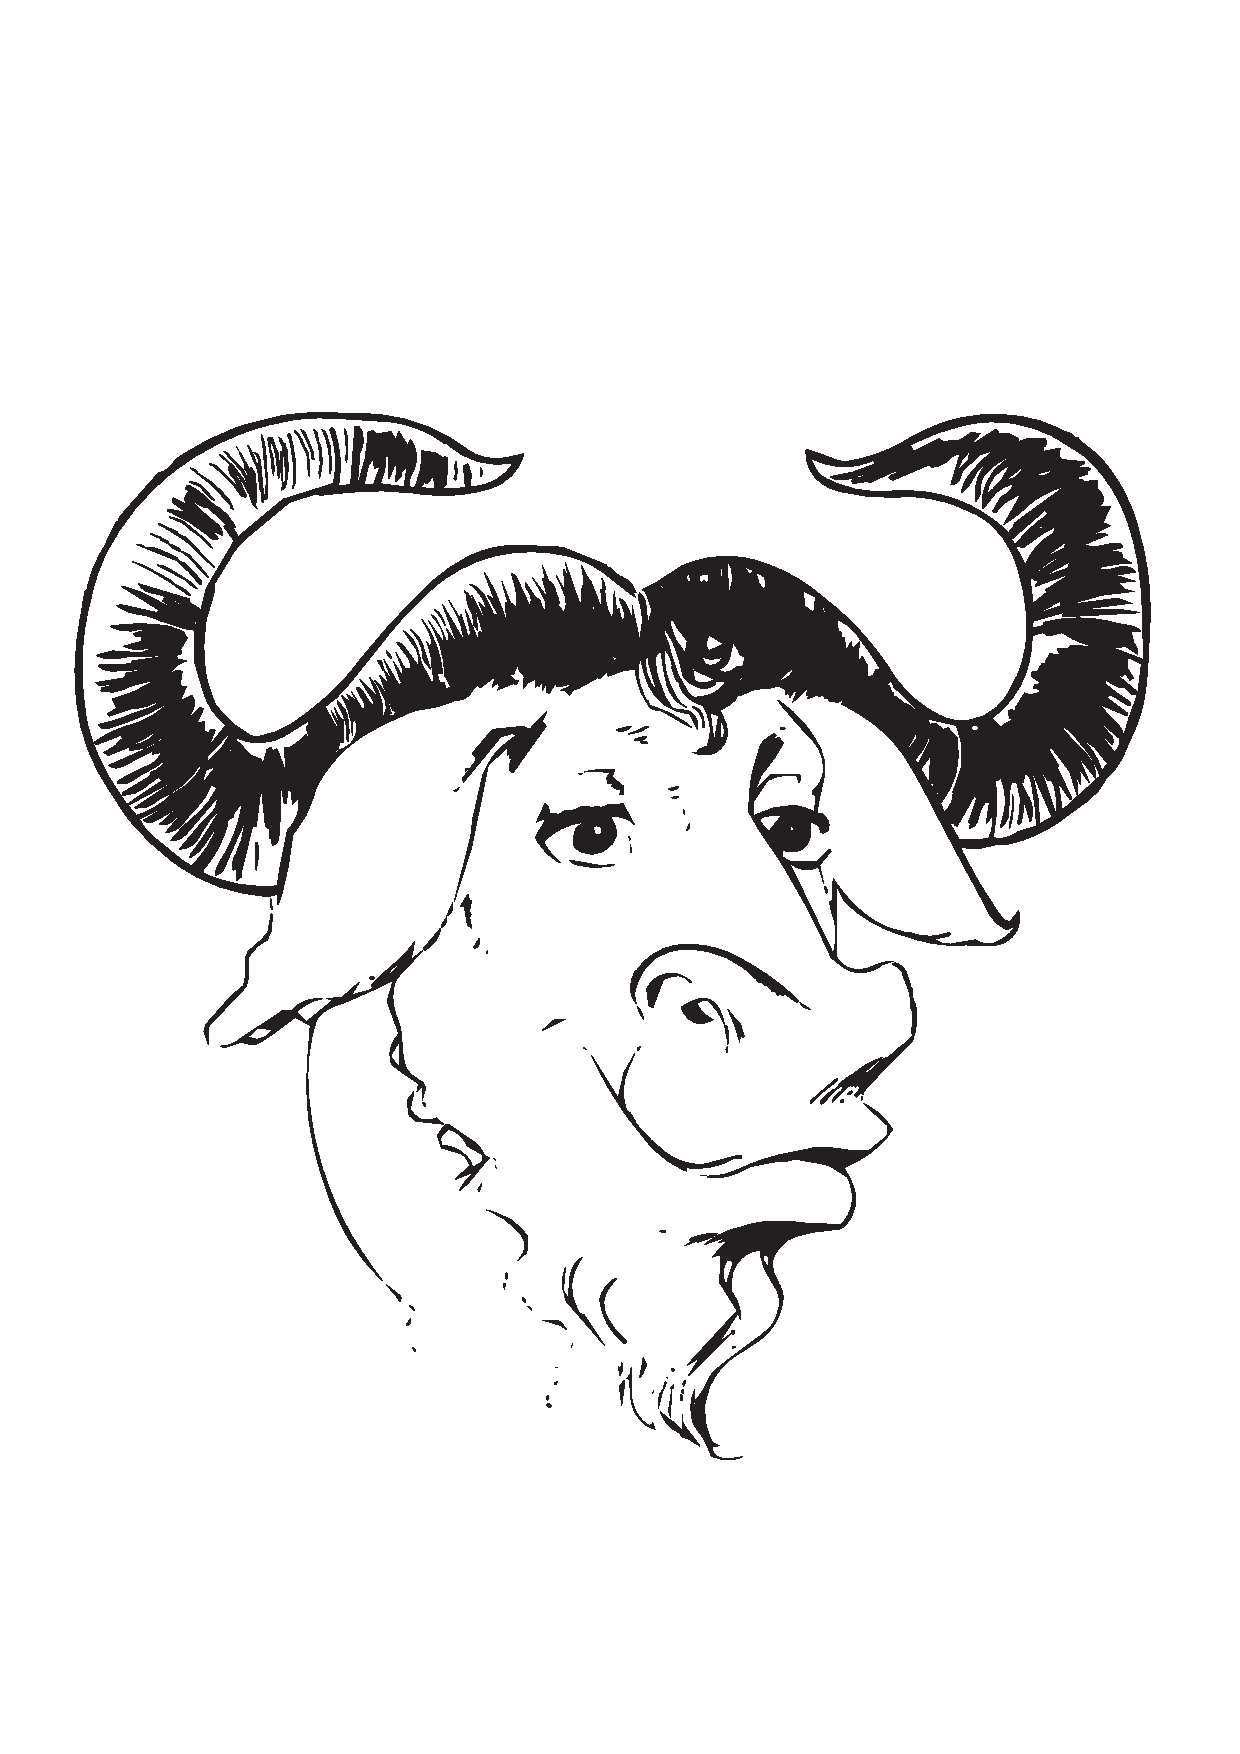
\includegraphics[width=3cm]{images/gnu-head}
\end{InText}

�����\sty{graphicx}�ѥå��������Ϥ��줿�ѥå��������ץ�����
���äơ�ĥ����ޤ�������ͥ���̤��Ѥ��ޤ��Τǡ�
\Option{dvips}����ꤷ�Ƥ������EPS����\Option{dvipdfmx}��
���ꤷ�Ƥ������PDF��ĥ����ޤ��褦�ˤʤ�ޤ���
���Τ褦��\sty{graphicx}���ɤ߹��ߤλ������ѹ���������Ǥ���

\begin{InText}
%\usepackage[dvips]{graphicx}  % dvipsk   ��
\usepackage[dvipdfmx]{graphicx} % Dvipdfmx ��
\end{InText}


\subsection{��ݡ��ȡ���ʸ�ˤ�����ޤ�ĥ�����}

��ݡ��Ȥ���ʸ�ʤɤǿޤˤ�\K{�޸��Ф�}���դ���\K{���·��}��
����Τ�˾�ޤ����Ȼפ��ޤ��Τǡ����Τ褦�˻Ȥ����ˤʤ�ޤ���

\begin{InText}
\begin{figure}[htbp]
 \begin{center}
   \includegraphics[width=10cm]{images/file.eps}
   \caption{�޸��Ф�}\label{fig:samplefig}
 \end{center} 
\end{figure} 
\end{InText}

����������������
�񤯤Τ����ݤʤΤǼ��Τ褦�ʿ��Ѥ�\env{myfig}̿���
�������ޤ���

\begin{InText}
\newcommand{myfig}[4][width=.8\linewidth]{%
\begin{figure}[htbp]%
   \centering\includegraphics[#1]{#2}%
   \caption{#3}\label{fig:#4}%
\end{figure}}
\end{InText}

���Τ褦��������Ƥ����м��Τ褦�˴�ñ�˻Ȥ��ޤ���

\begin{InText}
�ʾ�ιͻ������~\ref{fig:sample}�Τ褦�ʿޤ������롥
\myfig[width=100pt,clip]{images/file.eps}{�ޤ�ĥ����ߤ���}{sample}
\end{InText}

��ư�Τοޤ�DVI�ե�����˽��Ϥ����Ȥ��˻פ�����ʤ����ޤ�ι�򤷤�
���Τǡ��פ��̤�ξ��˿ޤ����֤���ʤ��Ƥ�ʢ��Ω�Ƥʤ��Ǥ���������
���⤽���ɽ���Ф���\yo{�嵭�οޤϲ���}�Ȥ�\yo{�����οޤϲ���}�Ȥ���ɽ��
�ϴְ㤤�ǡ����Ƥο�ɽ��\yo{��~3.1�ϲ���}�Τ褦���ֹ�ǻ��Ȥ��ޤ����Ǥ�
��������Ͽ�ɽ���ɤΤ褦�ʾ���ιΩ�äƤ⺤��ʤ��Ϥ��Ǥ���

%HOGE 1037 ������������

\subsection{����Ū�ʲ����κ����ȳ���}\seclab{excel:kowaza}

\LaTeX ��\Dvipdfmx ���Ѥ�����ǡ�JPEG, PNG, BMP, EPS, PDF ���β�����ĥ��
���������ǽ�Ǥ������������������ץ������ˤ�äƤϤ����η����β����ե�
�����\Z{�񤭽Ф�}���Ѵ��ˤ��б����Ƥ��ʤ���礬����ޤ������ξ��Ϥ���
����Υץ�����फ�顤\Z{���ۥץ��}���Ф��Ʋ��������Ƥ���������EPS��
PDF����¸����Τ���û�ˤǤ�����ˡ�Ȥʤ�ޤ���

Windows �Ǥ���� \Prog{PrimoPDF}���Υե꡼���Ѵ��ץ�����ब����ޤ���
Mac~OS~X�Ǥ����OS���Τ�Τ�PDF�Ǥν񤭽Ф����б����Ƥ��ޤ���%\unixos �Ǥ�

���ߤ��Ȥ��δĶ���\Prog{Adobe Acrobat}��������ϡ�Acrobat����Ѥ�
�Ƥ��������ƹ����ޤ���

\subsection{�ץ��������ͭ�ν���}\seclab{picture:program}

����γ����ץ�����फ�饰��դ�����������Ȥ��ˤϴ��Ĥ����Ĥ�ɬ
�פǤ���\secref{excel:kowaza}�Ǥ�ĥ���������¾�Υ��ץꥱ�������
�Ǥ�Ŭ�ѤǤ����礬¿���Τǡ��嵭����ˡ���ƤߤƤ���������

�ɤΥץ���������Ѥ��Ƥ��Ƥ�ǽ�Ū�˽��Ϥ����������Υ������򸵤Υץ���
���¦��Ĵ�ᤷ�Ƥ���{\LaTeX}��ĥ�����褦�ˤ��������⾯�ʤ��Ǥ��礦��
\sty{graphicx}�ѥå������γ���̾���Ȥ��Ȱ����ʼ�������ޤ����ƥץ�
�����ˤ�����������ˡ�ϰʲ����̤�Ǥ�\footnote{�ץ������ΥС�������
��äƤϴ�ʬ�����ˡ���ۤʤ�Ȼפ��ޤ���}��

\begin{description}
\item[\prog{Illustrator}]
  ��ǽ�Ǥ����ʸ���ϥ����ȥ饤�󲽤��ޤ���
  Adobe PDF �θߴ����Ǥ� \win{Acrobat 4 (PDF 1.3)}����ꤹ��
  �褦�ˤ���ȡ����꤬ȯ�����Ť餤�Ȼפ��ޤ���
  �ġ���С���\win{��̾����¸}�ǥե����������\qu{Adobe 
  PDF}�Ȥ�����¸���ޤ���PDF�����Ǥ���¸���ץ�����\yo{����͡�
  ���������}��\K{�����å��򳰤���}��\yo{����}�Ϥ��ʤ��褦��
  ���Ƥ���������\Prog{Illustrator}�ξ����ѻ極�������ڤ�ȴ����
  �ޤ���ΤDz��餫����ˡ��\Prog{Adobe Acrobat}�� \cmd{includegraphics}
  ̿��� \option{trim} ���ץ����ˤ��ڤ�ȴ����Ԥ�ɬ�פ�����ޤ���
\item[\Prog{Photoshop}]
  \win{�ե�����}��\win{ʣ������¸}������\yo{��¸����}
  ��\qu{Photoshop PDF}�ˤ�����¸���ޤ����ӥåȥޥåײ����ϰ��̤��ʤ��ۤ�����
  ���ʼ����ɤ��褦�Ǥ���
\item[Gnuplot] �ե꡼�Υץ��åȥ��եȤ� \PS, \Y{PSTricks}, \Prog{Tgif},
  \Prog{Illustrator}, \Y{eepic}, \Prog[MetaFont]{\MF},
  \Prog[MetaPost]{\MP}����¿���η����Dz����ν񤭽Ф��򥵥ݡ��Ȥ��Ƥ��ޤ���
  \Prog{Octave}��\Prog{MATLAB}�����GPL�ο��ͱ黻���եȤ� Gnuplot ���Ȥ�
  ��ȯ����Ƥ��ޤ��ΤǼ��� Gnuplot �ξ��ȤۤȤ��Ʊ���Ǥ���\Y{eepic}
  �ѥå��������н褹��ˤϡ��㤨�� Gnuplot ¦�Ǽ��Τ褦�ˤ��ޤ���

\begin{InText}
set output 'plotfile1.tex'\\
set term eepic rotated dashed\\
plot x
\end{InText}

����ȡ������ȥǥ��쥯�ȥ��\fl{plotfile1.tex}����������ޤ����顤
\Y{eepic}�ѥå����������Ѥ��ơ�\LaTeX �θ���¦�Ǽ��Τ褦�˵��Ҥ��ޤ���

\begin{InText}
\documentclass[dvipdfmx]{jsarticle}
\usepackage{graphicx,color,epic,eepic,amssymb}
\begin{document}
\input{plotfile1}
\end{document}
\end{InText}

  ���ξ��� \sty{graphicx}, \Y{epic}, \Y{eepic}, \Y{amssymb}�ѥå�������
  ɬ�פȤ��Ƥ��ꡤ\C{input} ̿��ǥץ��åȤ��줿����� \fl{plotfile1.tex}
  ���ɤ߹���褦�ˤ��Ƥ���ޤ���
 \item[R] 
  \index{GNU!\zdash GPL}
  \Z{GPL}�����ײ��ϥ��եȤ� \PS, PDF, \Prog[PicTeX]{Pic\TeX}, \Prog{Xfig}, 
  PNG, JPEG ���ν񤭽Ф��򥵥ݡ��Ȥ��Ƥ��ޤ���

\begin{InText}
pdf()\\
plot(rnorm(10))\\
dev.off()
\end{InText}  

  �嵭�Τ褦��\Prog{R}��������Х�����ȥǥ��쥯�ȥ��PDF������
  ����� \Fl{Rplots.pdf}����������ޤ���
\item[Tgif] \Person{William Chia-Wei}{Cheng}�ˤ��\Z{QPL}�����襽�եȡ�EPS
  �� PDF �������б����Ƥ��ޤ���PDF�˴ؤ��Ƥ�\GS ���γ����ץ�������ɬ��
  �Ȥ��ޤ���
 \item[Mac OS X] Mac OS X �ξ��ϴĶ����Τ� PDF �˴�Ϣ������ǽ����ä�
 ���뤿�ᡤPDF �����ǽ񤭽Ф����ˤ�� \LaTeX �˲�����
 ����������Ǥ��ޤ���\Prog{Keynotes}, \Prog{Pages}, \Prog{Grapher},
 \Prog{OmniGraffle}����������ξ����˥塼�С��� \win{�ե�����} ��
 \win{�񤭽Ф�} �� \win{PDF} �����򤹤���� PDF �Ȥ�����¸�Ǥ���
 ����\Prog{�ץ�ӥ塼}�� \win{����ġ���} �ˤ�ä��ڤ�ȴ�������ΰ��
 ���򤷡������ \win{���ԡ�} ������ \win{����åץܡ��ɤ��鿷����
 ��} �Ȥ����PDF�������ڤ�ȴ����Ǥ��ޤ���

\zindind{PDF}{��Mac OS X}%
\item[\Prog{Mathematica}]
  �ġ���С�����\win{�ե�����}��\win{�ü�ʷ�������¸}������
  \win{TeX(X)}�����Ӥޤ��� ��������ȿ����䥰��դʤɤ���ưŪ��
  {\LaTeXe}��������¸����ޤ����ޤ�����դ�EPS������{\fl{
  filename.eps}}�Ȥ���̾������¸����ޤ���{Mathematica}�ξ��
  ���Ϥ����EPS������\Z{�Х���ǥ��󥰥ܥå���}�������
  ���Ϥ���ʤ���������Τ�{\LaTeX}�������������Ǥ��ʤ����
  ������ޤ������Ϥ��줿\fl{filename.eps}�Ȥ����ե������
  �ƥ����ȥ��ǥ����dz����м��Τ褦�ʵ��Ҥ�����ޤ���

\begin{InText}
%%BoundingBox: 91.5625 3.1875 321.938 190
\end{InText}

  ����ϲ�����ʿ�̾�
  �Τɤ������֤��뤫����ꤹ���Τǡ�������
  2����ʿ�̾�λ�����$x_0$��$y_0$��������$x$��
  $y$���б����ޤ����ޤ����̾�Ϥ����ͤ������ͤ�
  �侩����ޤ����嵭�ο��ͤ�ͼθ�������������
  ľ���Ƽ�����Ǥ���������
\item[\Prog{MATLAB}]
  ����դ�ɽ�����Ƥ���MATLAB�ץ������Υ�����ɥ���
  �ġ���С��ˤ��� \win{�ե�����} ���� \win{�������ݡ���} ��
  ���ӡ��ե�����μ����\qu{EPS Level 2}�ˤ���Ǥ�դ�̾��
  ��Ĥ�����¸���ޤ���{Illustrator}�����Ǥν��Ϥ⥵�ݡ���
  ����Ƥ��ޤ��Τǡ��������ξ��ϥ���դ��Խ��Ǥ��ޤ���
\end{description}

����Ū�ˤ� PDF �ˤ����Ѵ����Ƥ���� \Prog{Adobe Acrobat} �ˤ���Խ���
��ǽ�Ȥʤꡤ����� \Dvipdfmx ���Ѥ���д�ñ�˲�����ĥ���������Ǥ��ޤ���
����PDF�˲������Ѵ�����ȡ�����PDF�ե�������Խ���\prog{Adobe Acrobat}��
�褦��PDF�Խ��ץ�����बɬ�פȤʤ�ޤ������Τ��ᡤ������Ĵ���˴ؤ��Ƥ�
���γ����ץ������¦�ǹԤ��褦�ˤ��ƤߤƤ���������
\zindind{PDF}{���Խ�}%

\section{�ޤ�ĥ����ߤκݤι���}


\subsection{�ޤ���IJ����¤٤�}
2���Ȥξ��Ϥ��Τ褦�ʻ��Ϥ���ޤ��󤬡�1���Ȥξ��ϰ�Ĥοޤ����Ǥ�
ξ�Ƥ������Ƥ��ޤ��ΤǤ�������Ĥοޤ�\qu{(a)}��\qu{(b)}�Ȥ�������������
�Ȥ�������ޤ������Τ褦�ʤȤ���\Env{minipage}�Ķ���Ȥ��ޤ����ʲ��Τ褦
�����Ϥ�����⤢��ޤ���

\C*{hfill}%
\begin{InText}
\begin{figure}[htbp]
  \begin{minipage}{.47\textwidth}
      \centering%�����˿�(a)�������
      {\small (a) �����$c=0.6$}
  \end{minipage} \hfill
  \begin{minipage}{.47\textwidth}
      \centering%�����˿�(b)�������
      {\small (b) �����$c=1.0$}
  \end{minipage}
  \caption{1���ȤDz��˿ޤ�����¤٤�}
\end{figure}
\end{InText}

ξ���οޤ��ֹ���̤ˤ������Ȥ���Ʊ�ͤ˵��Ҥ��ޤ���
��İʾ岣���¤٤�Ȥ����ˤ�\Person{Steven Douglas}{Cochran}�ˤ��
\Y{subfigure}�ѥå�������Ȥ��Ȥ���ñ�˵��ҤǤ�����ˤʤ�ޤ���

\begin{figure}[htbp]
  \begin{minipage}{.47\textwidth}
      \centering
      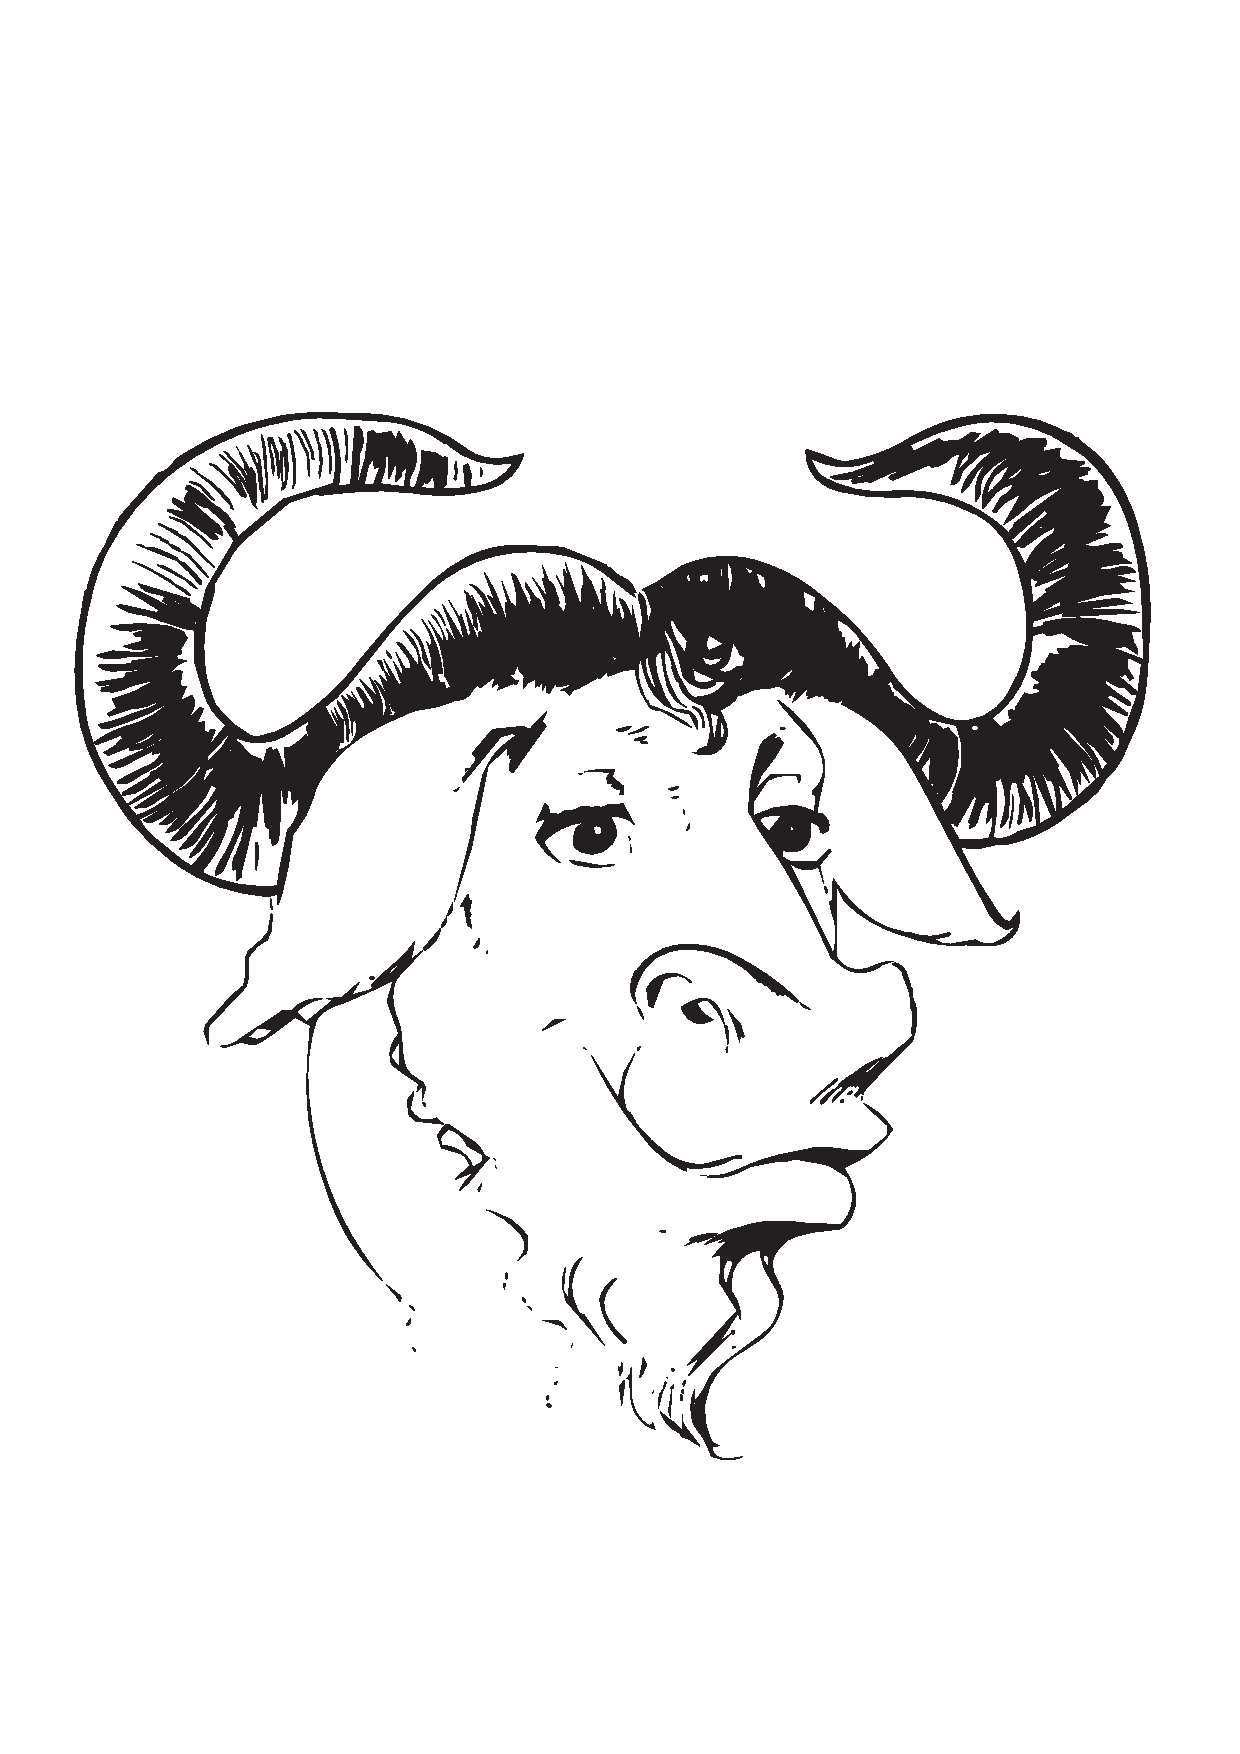
\includegraphics[width=2cm]{images/gnu-head}\\
      {\small(a) ����� $c=0.6$}
  \end{minipage}
\hfill
  \begin{minipage}{.47\textwidth}
      \centering
      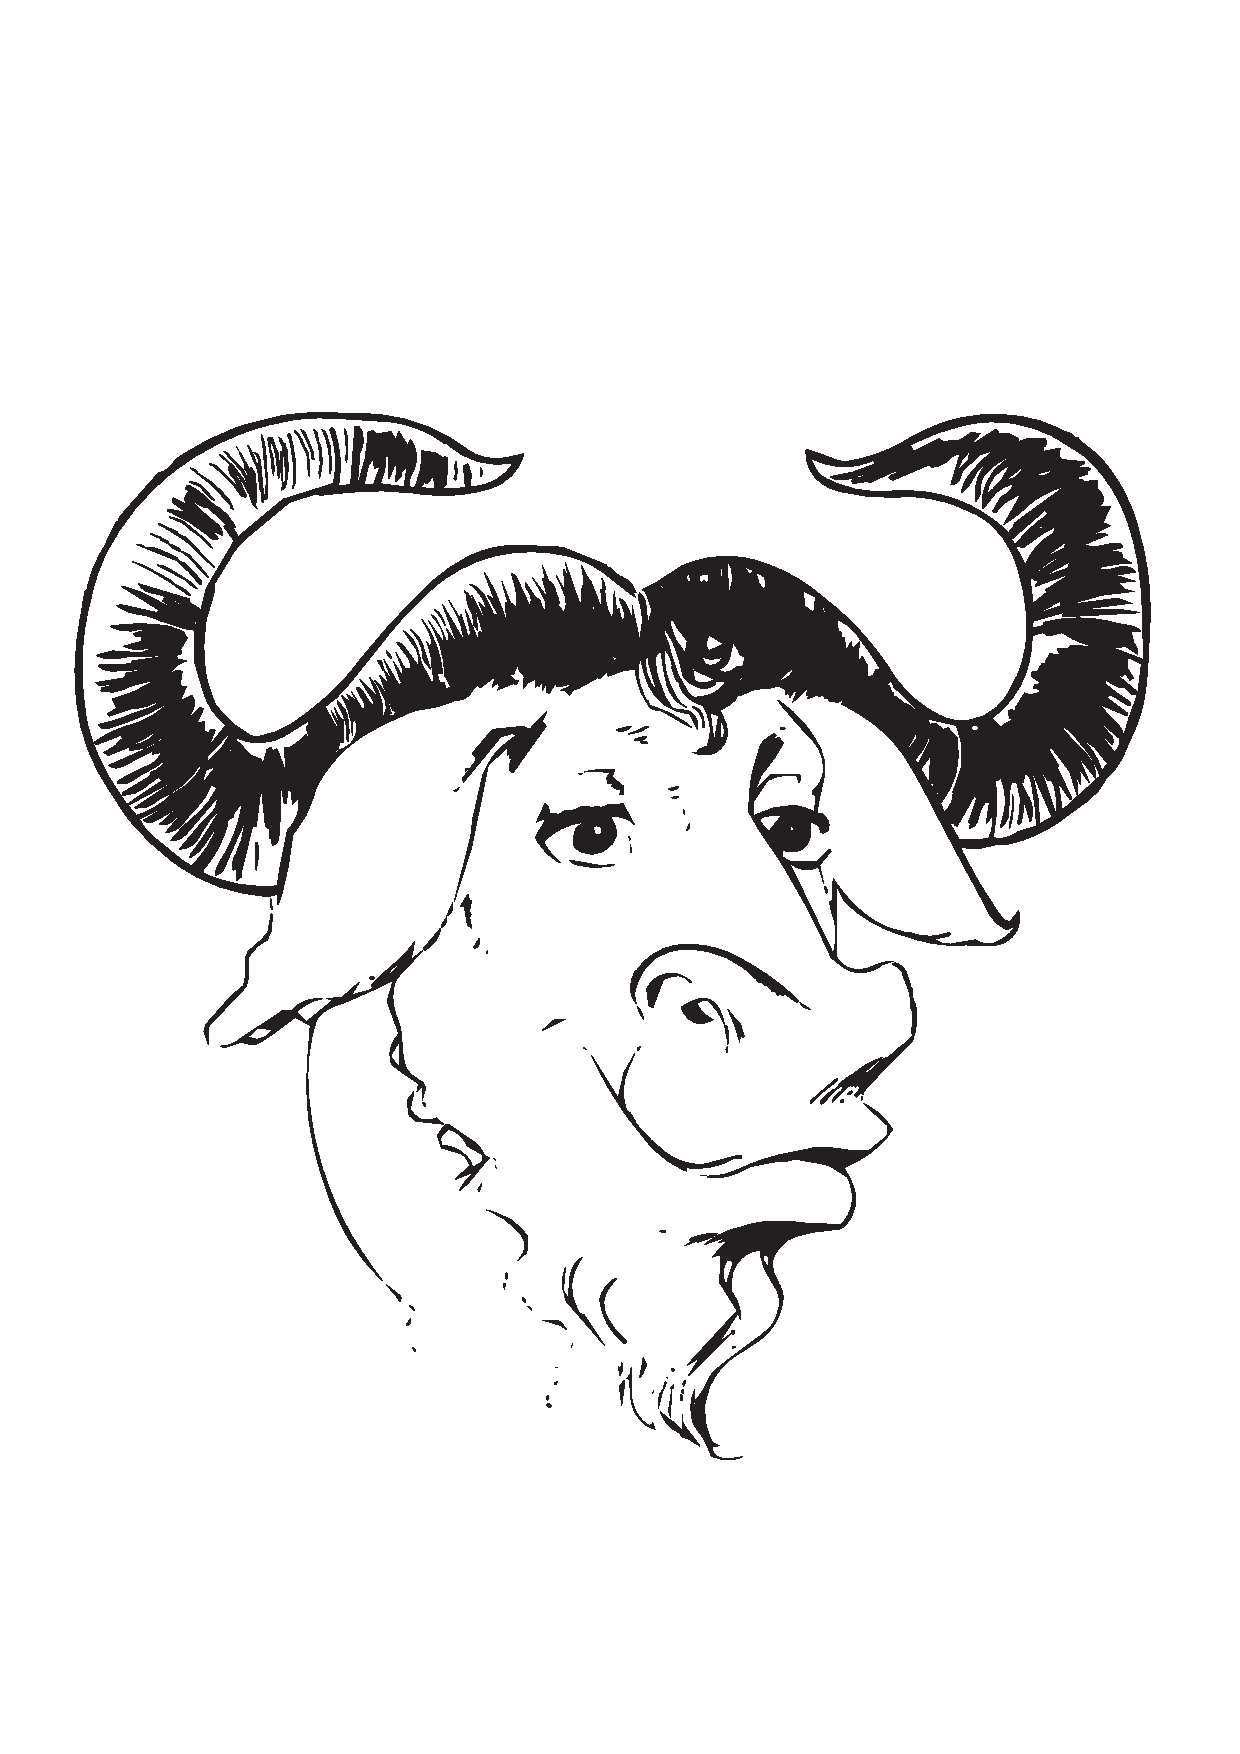
\includegraphics[width=2cm]{images/gnu-head}\\
      {\small(b) ����� $c=1.0$}
  \end{minipage}
  \caption{1���ȤDz��˿ޤ�����¤٤�}
\end{figure}


\begin{Prob}
����Ķ��ʤɤˤ����뤽�λ�����ʸ�������ݻ����Ƥ��� \Cmd{linewidth}
�Ȥ���Ĺ��������ޤ�������Ĺ����Ȥ���
���δĶ��ˤ�����ʸ�������äѤ��οޤ�ĥ�����Ȥ�����
��Ǥ���褦�ˤʤ�ޤ���

 �������Ϥ�ºݤ˼�ʬ�ǥ����ץ��åȤ������η�̤��̣���Ƥ���������
\begin{InOut}
\begin{quote}
  linewidth $=$ \the\linewidth\par
  \begin{quote}
    linewidth $=$ \the\linewidth
  \end{quote}
\end{quote}
\end{InOut}

����ˤ��Ԥ�Ⱦʬ���٤�Ĺ���ǿޤ�ĥ�����ʤ�С����Τ褦��
����Ǥ���ȹͤ�����Ǥ��礦��

\begin{InTeX}
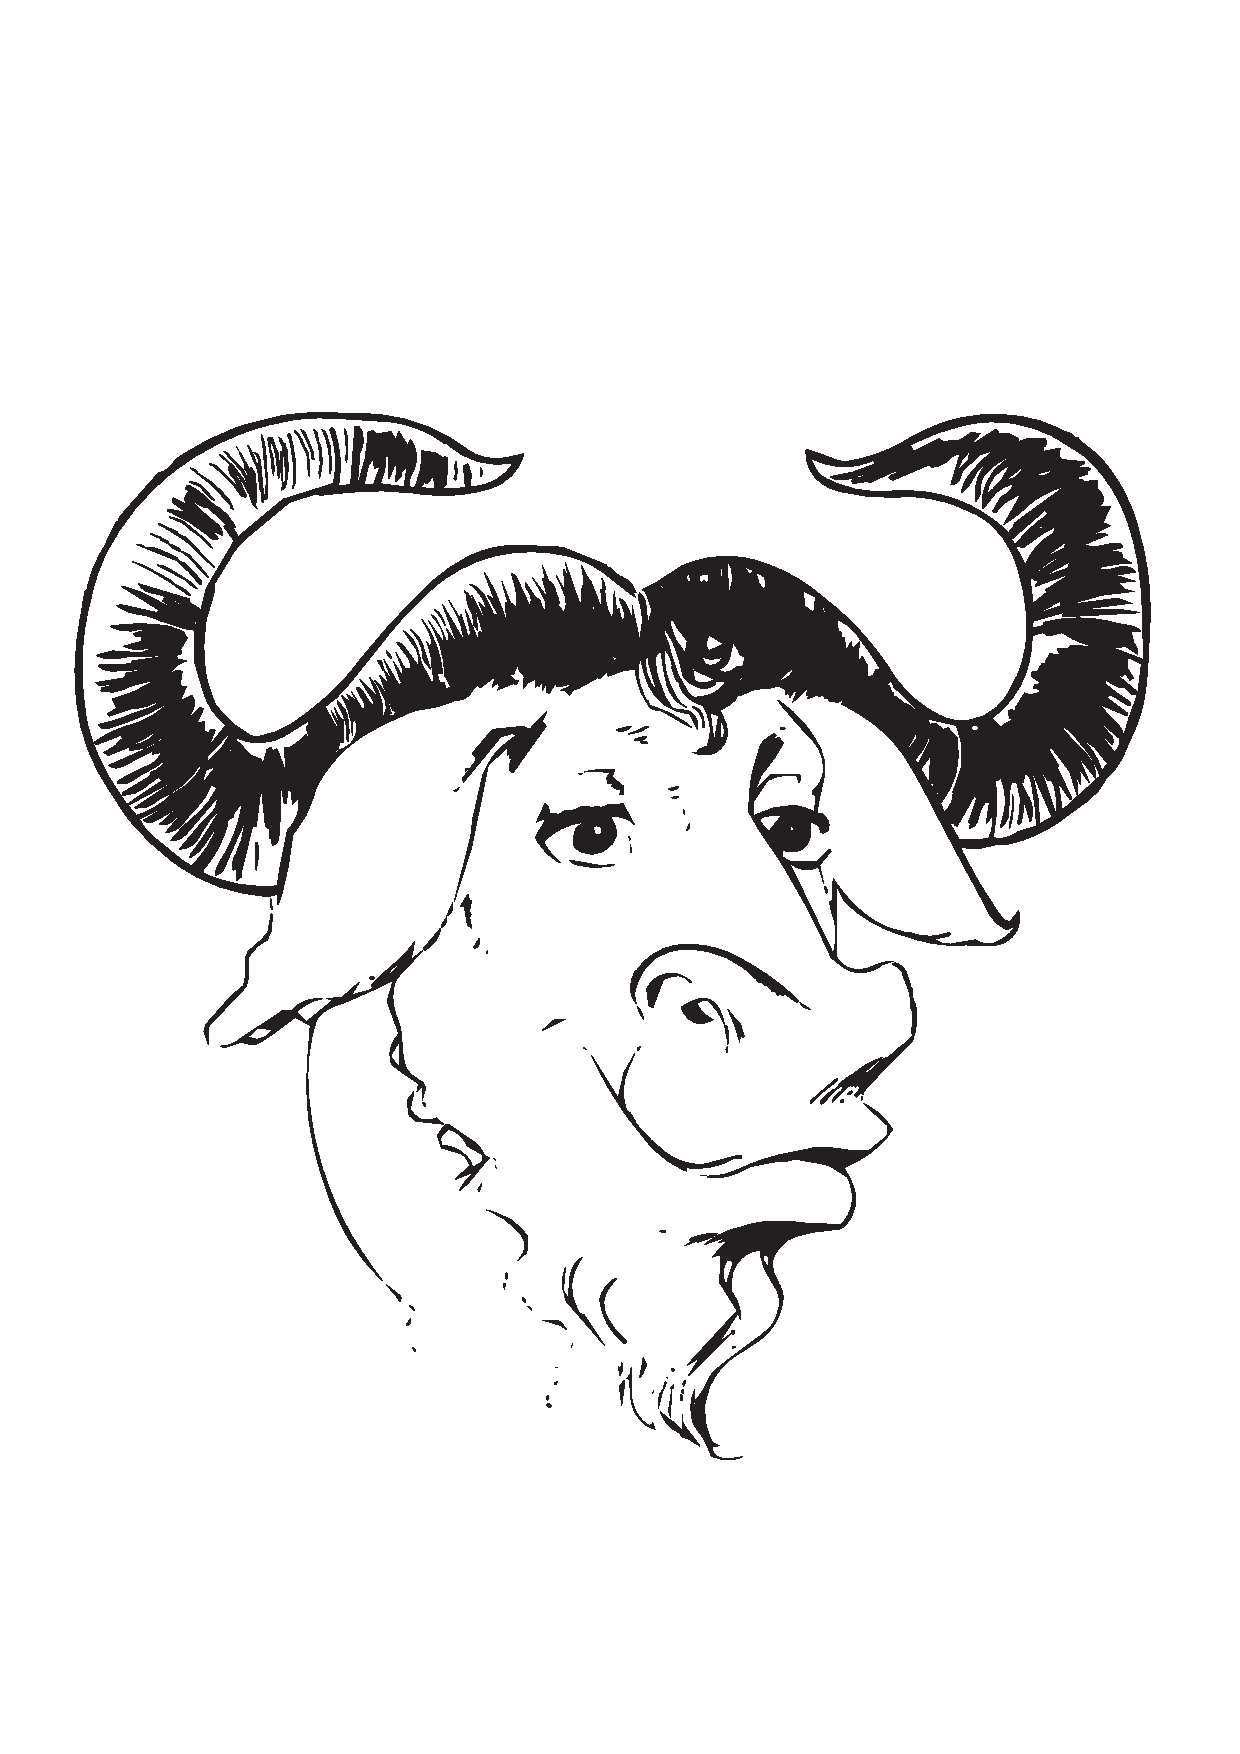
\includegraphics[width=.47\linewidth]{images/gnu-head}\\ 
\end{InTeX}
\end{Prob}

\begin{Prob}
��ɽ��ĥ�������� \C{includegraphics}̿������
�ǥ��쥯�ȥ�̾�򵭽Ҥ���Τ����ݤʾ��� \C{graphicspath}
̿�᤬�Ȥ��ޤ���

\begin{Syntax}
 \C{graphicspath}\pa{�ǥ��쥯�ȥ�Υꥹ��}
\end{Syntax}

���� \fl{images} �� \fl{pictures} �ǥ��쥯�ȥ�˲�����
��¸����Ƥ���Ȥ���С�\cmd{graphicspath}�ϼ��Τ褦��
�Ǥ��뤫���ºݤ˥����ץ��åȤ������η�̤��̣���Ƥ���������

\begin{InTeX}
\graphicspath{{images/}{geolay/}}
\end{InTeX}
\end{Prob} 

\subsection{������ʸ�����ɲä���\zdash\textsf{labelfig}}

\zindind{����}{�ؤ�ʸ�����ɲ�}%
���Խ����񤷤������ե����롤�㤨�� EPS �ե�����ξ��ʸ���ʤɤΥ�٥��
�ɲä�������礬����ޤ�������ˤ� \Person{Raymond}{S\'eroul} ��
\Person{Laurent}{Siebenmann} �ˤ�� \Y{labelfig} �ѥå��������Ȥ���
�Ǥ��礦��
\begin{Syntax}
\C{SetLabels} \\
\va{�����ξ��ɽ����������٥�}\\
\C{endSetLabels}\\
\C{ShowGrid} \pp{ɬ�פ˱�����}\\
\C{strut}\C{AffixLabels}\va{���֤������}
\end{Syntax}
\C{SetLabels} ���� \C{endSetLabels} ����Dz����ξ��ɽ����������٥��
���ꤷ�ޤ�����٥���ɲä���Ȥ���ɬ�פ˱����� \C{ShowGrid} ���ޥ�ɤ�
��ɸ��ɽ�����ޤ���\C{AffixLabels} �ΰ��������֤��٤���������ꤷ�ޤ���
��٥�ϼ��ν񼰤˽��ä��ɲä��ޤ���
\begin{Syntax}
\va{���ֻ���}\string(\va{0--1}\string*\va{0--1}\string) \va{��٥�} \verb|\\|
\end{Syntax}
��ɸ����� \verb|(0.5*0.3)| �Τ褦�� 0 ���� 1 ���ϰϤǻ��ꤷ�ޤ���
\va{���ֻ���}�ˤ� ��ľ������·���Ǥ� \C{T}��\C{E}��\C{B}��
��ʿ�����Ǥ� \C{L}, \C{R} ��̵����\pp{̵���������ˤʤ�}��ξ����
�Ȥ߹�碌�ƻȤ������Ǥ��ޤ���

\C{ShowGrid} �ˤ�äƥ���åɤ�ɽ������Τϸ��Ƽ�ɮ�ʳ������ǡ�
�������ˤ�ɽ�����ʤ��Ȥʤ�� \Option{draft} ���ץ�������Ѥ��ޤ���
��������\sty{graphicx} �ѥå������ˤ�ä��ɤ߹���Ǥ�������˴ؤ��Ƥ�
\Option{draft} ���ץ����ͭ���ˤʤäƤ���Ȥ��Ǥ� \Option{final} 
���ץ������դ����Ȥ��Τ褦�����֤��Ƥ�餤�����Τǡ��㤨��
���Τ褦�ˤ��ޤ���

\begin{InText}
% ����åɤ�ɽ��������Τ� draft �λ������ˤ�����ɤ����Ȥˤʤ�
%\documentclass[draft,a4j,11pt,papersize]{jsarticle}
% �������ˤ� draft ���ץ�����������ɤ����Ȥˤʤ롥
\documentclass[a4j,11pt,papersize]{jsarticle}
% graphicx �ѥå������ˤ� final ���Ϥ��ơ����ĤǤ�ޤ�ɽ�������
% �褦�ˤ���ȡ�labelfig ��Ĵ�����ưפˤʤ롥
\usepackage[final]{graphicx}
\usepackage{labelfig} 
\end{InText}

�㤨�м��Τ褦�����Ϥ������ \figref{labelfig} �Τ褦�ʽ��Ϥ�
�ʤ�ޤ���\C{GridLineWidth}���ޥ�ɤǷ��������������Ǥ��ޤ���

\begin{InText}
\begin{figure}[htbp]
\begin{center}
 \GridLineWidth{.2pt}
 \SetLabels 
  \T\L(.8*.45) ɡ\\
  \T\L(.2*.9) ���γ�\\
  \T\L(.7*.9) ���γ�\\ 
  \T\L(.75*.3)  ��\\ 
  \T\L(.65*.1) ɦ\\ 
  \T\L(.3*.6) ����\\ 
  \T\L(.7*.6)  ����\\ 
 \endSetLabels
 \ifdraft
   \ShowGrid
 \fi
 \strut\AffixLabels{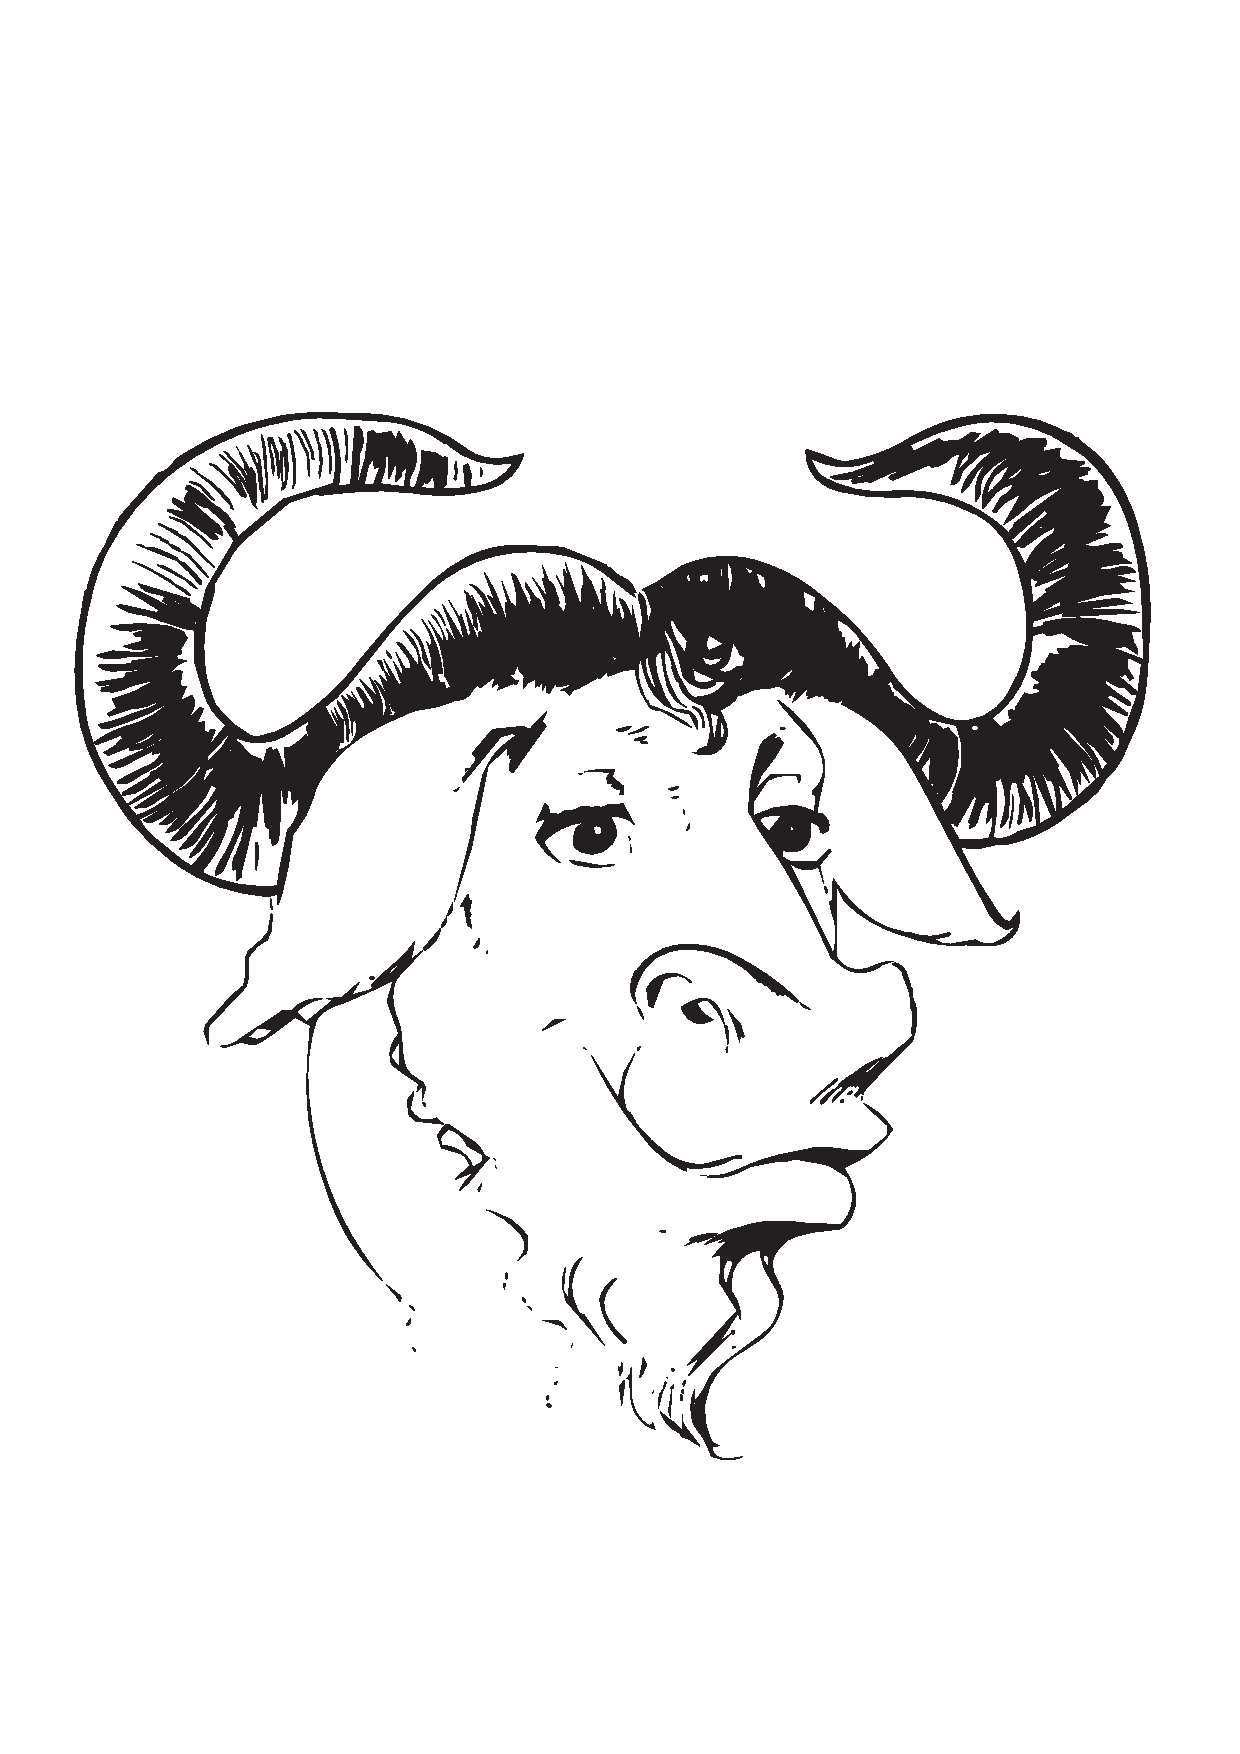
\includegraphics{images/gnu-head}}%
 \caption{\Y{labelfig} �λȤ���\label{fig:you}}%
\end{center} 
\end{figure} 
\end{InText}

\begin{figure}[htbp]
\begin{minipage}{.49\linewidth}
 \GridLineWidth{.2pt}
  \SetLabels 
  \T\L(.8*.45) ɡ\\
  \T\L(.2*.9) ���γ�\\
  \T\L(.7*.9) ���γ�\\ 
  \T\L(.75*.3)  ��\\ 
  \T\L(.65*.1) ɦ\\ 
  \T\L(.3*.6) ����\\ 
  \T\L(.7*.6)  ����\\ 
  \endSetLabels
  \ShowGrid
  \strut\AffixLabels{%
    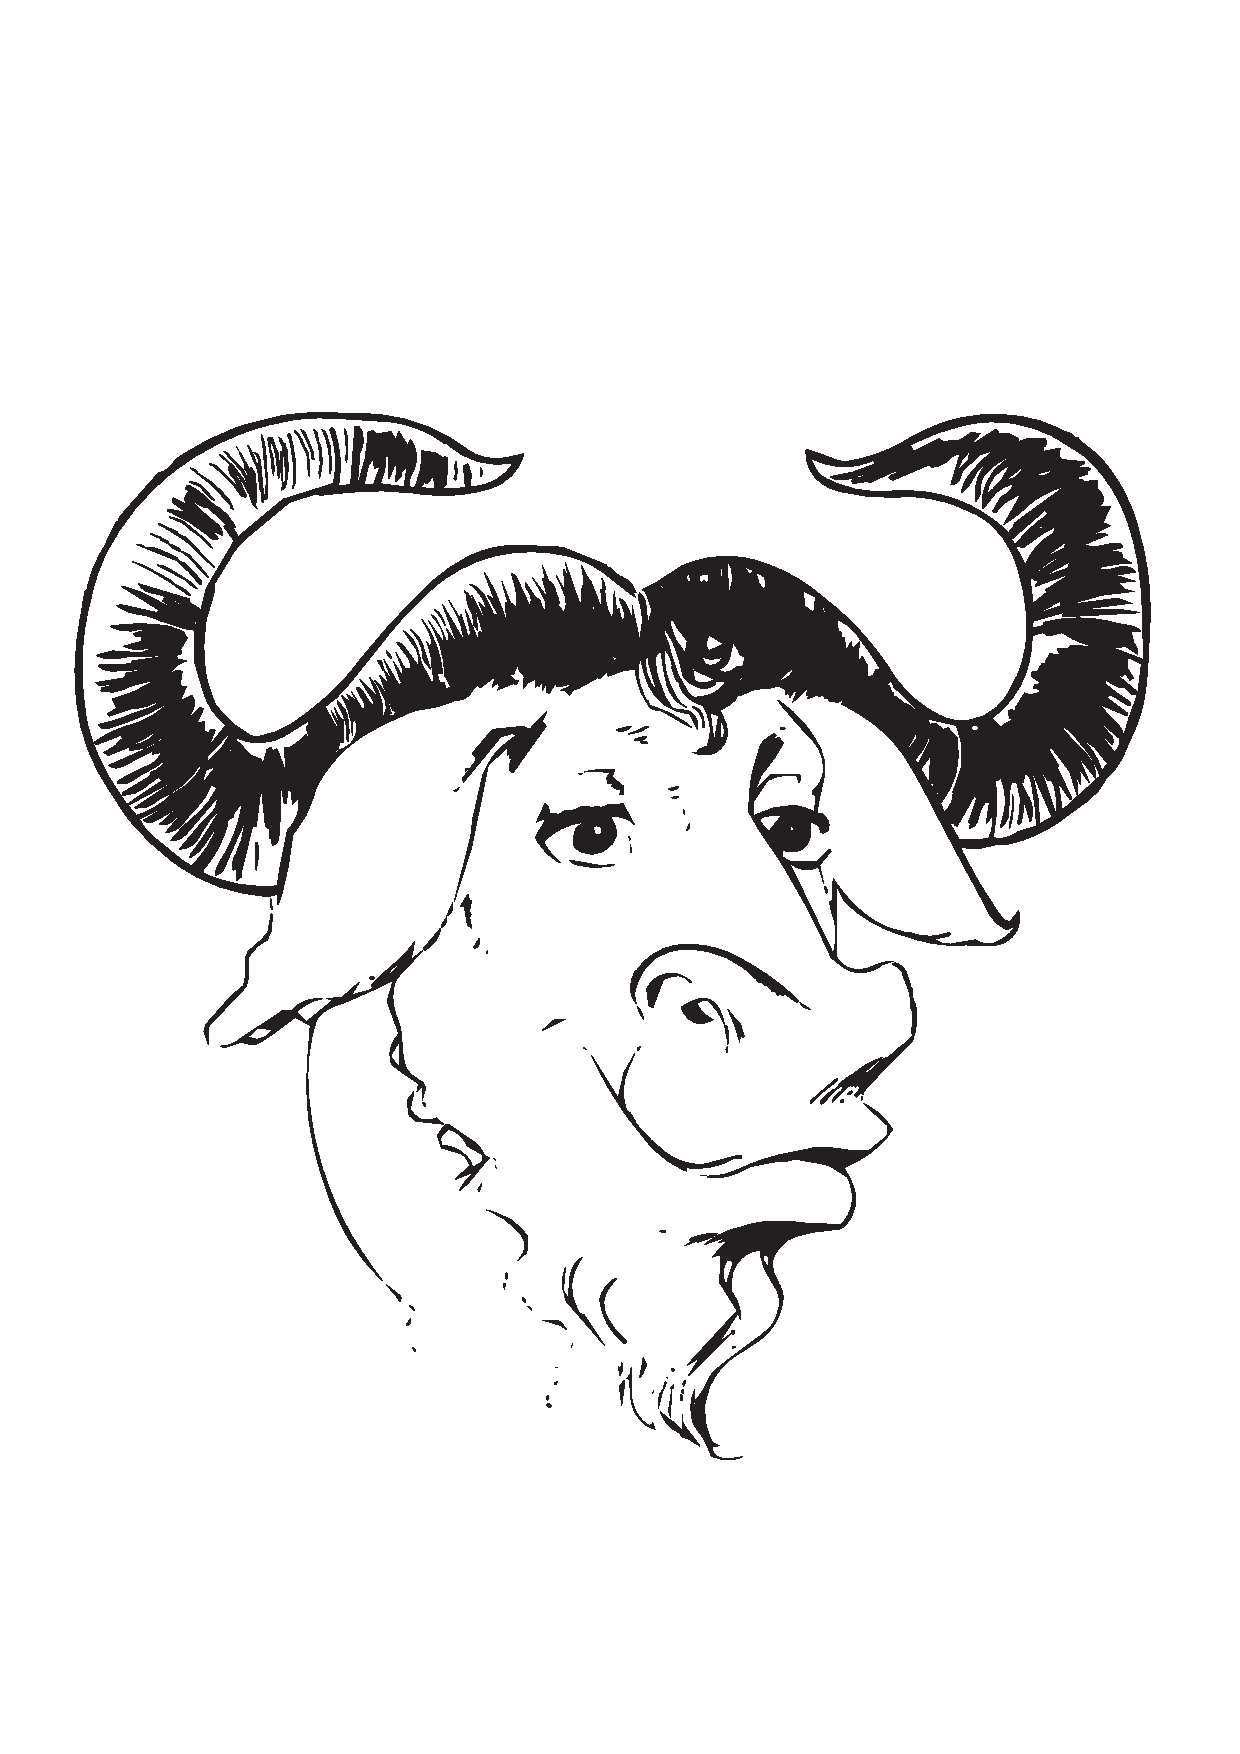
\includegraphics[clip,width=\linewidth]{images/gnu-head}}%
\end{minipage}
\hfil
\begin{minipage}{.49\linewidth}
  \SetLabels 
  \T\L(.8*.45) ɡ\\
  \T\L(.2*.9) ���γ�\\
  \T\L(.7*.9) ���γ�\\ 
  \T\L(.75*.3)  ��\\ 
  \T\L(.65*.1) ɦ\\ 
  \T\L(.3*.6) ����\\ 
  \T\L(.7*.6)  ����\\ 
  \endSetLabels
  \strut\AffixLabels{%
    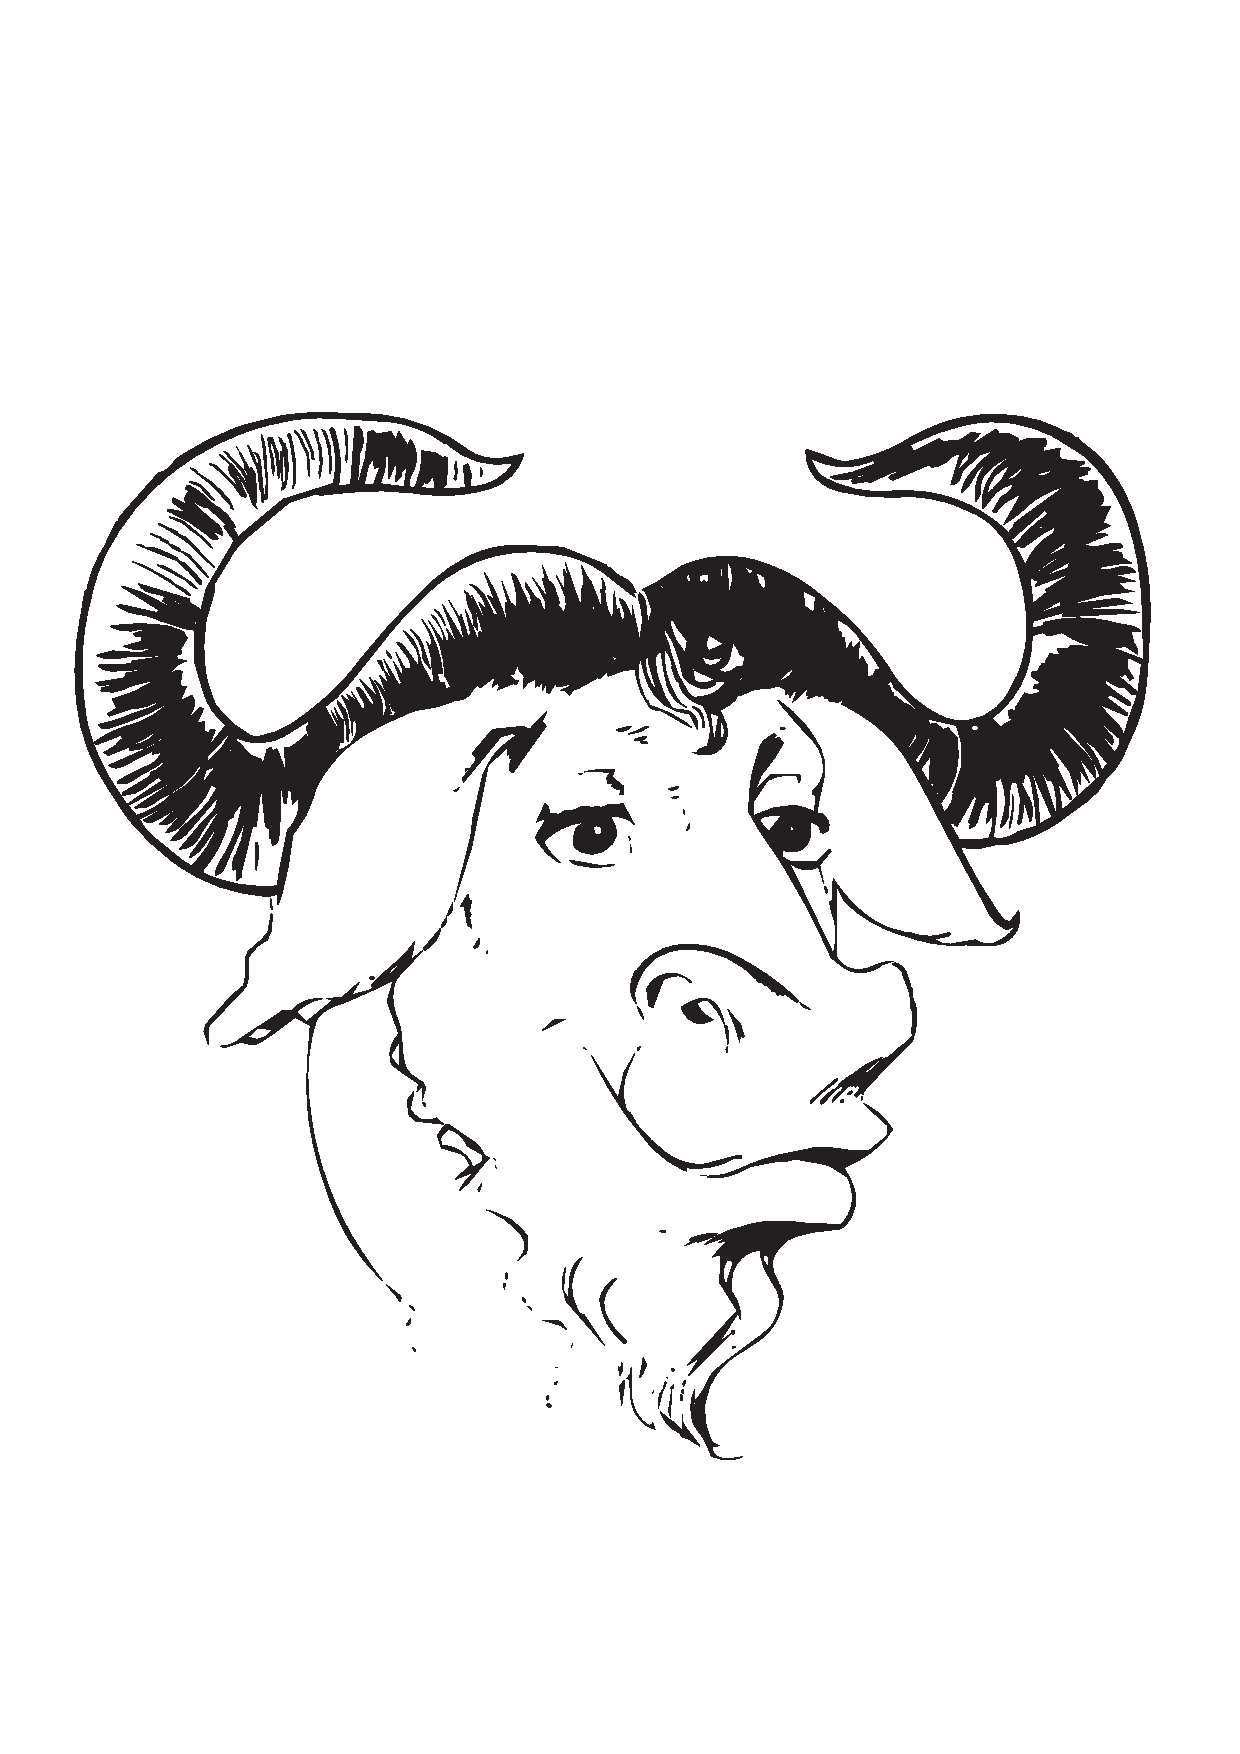
\includegraphics[clip,width=\linewidth]{images/gnu-head}}% 
\end{minipage}
 \caption{\sty{labelfig} �λȤ���\label{fig:labelfig}}%
\end{figure}


%��ݡ��Ȥ���ʸ�ʤɤǿޤˤ�\K{�޸��Ф�}���դ���\K{���·��}��
%����Τ�˾�ޤ����Ȼפ��ޤ��Τ�
%\begin{InTeX}
%\begin{figure}[htbp]
% \begin{center}
%   \includegraphics[width=10cm]{images/file.eps}
%   \caption{�޸��Ф�}\figlab{samplefig}
% \end{center} 
%\end{figure} 
%\end{InTeX}
%�Τ褦�˻Ȥ����Ȥˤʤ�Ǥ��礦������������������
%�񤯤Τ����ݤʤΤǼ��Τ褦�ʿ��Ѥ�\env{myfig}̿���
%�������ޤ���
%\begin{InTeX}
%\newcommand{myfig}[4][width=.8\textwidth]{%
%\begin{figure}[htbp]%
%   \centering\includegraphics[#1]{#2}%
%   \caption{#3}\figlab{#4}%
%\end{figure}}
%\end{InTeX}
%���Τ褦��������Ƥ����м��Τ褦�˻Ȥ��ޤ���
%\begin{InTeX}
%�ʾ�ιͻ������~\ref{fig:sample}�Τ褦��
%�ޤ������롥
%\myfig[width=100pt,clip]{images/file.eps}{�ޤ�ĥ����ߤ���}{sample}
%\end{InTeX}


%��ư�Τοޤ�DVI�ե�����˽��Ϥ����Ȥ��˻פ���
%���ʤ����ޤ�ι�򤷤ޤ��Τǡ��פ��̤�ξ���
%�ޤ���ϤǤ��ʤ��Ƥⵤ�ˤ��ʤ��Ǥ���������
%���⤽���ɽ���Ф���\yo{�嵭�οޤϤʤ�����}�Ȥ�
%\yo{�����οޤϤʤ�����}�Ȥ���ɽ���ϴְ㤤�ǡ�
%���Ƥο�ɽ��\yo{��~3.1�Ϥʤ�����}�Τ褦���ֹ��
%���Ȥ��ޤ����Ǥ���������Ͽޤ�ɽ���ɤΤ褦�ʾ���
%ιΩ�äƤ⺤��ʤ��Ϥ��Ǥ���

%�ޤʤɤ�ȿ���ײ���\kaku{90}��ž�����뤳�Ȥ�����Ǥ��礦��
%���ξ��� \Cmd{rotatebox}̿���Ȥ��ޤ���
%¾�ˤ�������̿�᤬����ޤ���
%\begin{Syntax}
%\Cmd{rotatebox}\opa{����}\pa{����}{����}
%\end{Syntax}
%����� \cmd{includegraphics}��Ǥ�հ�����
%\qu{\str{angle}}��Ȥä����Ȥ�Ʊ���Ǥ���
%\cmd{rotatebox}�Ͽޤ˸¤餺���������Ǥ�
%\Z{��ž}���ޤ���\va{����}�ι��ܤˤϰʲ��Τ褦��
%��Τ�����ޤ���
%\begin{description}
%\item[\str{origin=}\va{��٥�}] 
% ���Ǥ��ž���뤿��θ�������ꤷ�ޤ���%%
% ��\qu{\str l}����\qu{\str r}�����\qu{\str c}��
% ����\qu{\str t}������\qu{\str b}������Ǥ��ޤ���
%\item[\str{x=}\va{��}] 
%$x$�����θ����ΰ��֤�ľ��\va{Ĺ��}����ꤷ�ޤ���
%\item[\str{y=}\va{��}]
%$y$�����θ����ΰ��֤�ľ��\va{Ĺ��}����ꤷ�ޤ���
%\end{description}
%\indindz{��ž}{ʸ�����}%%%
%\begin{InOut}
%\rotatebox{70}{ʸ����ʤ�}��
%\rotatebox[origin=c]{60}{��ž�Ȥ�}��
%\rotatebox[origin=b]{50}{�ɤ��衩}
%\rotatebox{30}{����ݡ�}
%\end{InOut}

%���Ǥ�\K{����̾�}����ˤ� \cmd{scalebox}��
%�Ȥ��ޤ���\index{����}\index{�̾�}\indindz{����}{ʸ�����}
%\begin{Syntax}
%\Cmd{scalebox}\pa{���γ���Ψ}\opa{�Ĥγ���Ψ}\pa{����}
%\end{Syntax}
%\va{����Ψ}�ˤ�Ĺ������ꤷ�ޤ���\begin{InOut}
%\scalebox{2.3}{����̾�}\par
%\scalebox{3}[1]{����̾�}
%\end{InOut}
%
%���Ǥ�\K{ȿž}�ˤ� \cmd{reflectbox}��Ȥ��ޤ���
%\begin{Syntax}
%\Cmd{reflectbox}\pa{����}
%\end{Syntax}
%\begin{InOut}
%\reflectbox{ʸ�����ȿž}\par
%\reflectbox{���ϻ�}\par
%\scalebox{-1}[1]{�����ȿž}
%\end{InOut}
%
%�ꥵ�����ˤ� \cmd{resizebox}��Ȥ��ޤ���
%\begin{Syntax}
%\Cmd{resizebox}\pa{��}\pa{�⤵}\pa{����}
%\end{Syntax}
%���ǤΥꥵ�����������\va{��}�ˡ��⤵��\va{�⤵}�ˤ��ޤ���
%�ɤ��餫�����γ��硦�̾�Ψ�˹�碌�����Ȥ���\qu{\str!}��
%�Ȥ��ޤ���
%\begin{InOut}
%\resizebox{!}{1cm}{�ꥵ����}\par
%\resizebox{3cm}{!}{�ꥵ����}
%\end{InOut}

%�ʾ�� \cmd{rotatebox}��\cmd{scalebox}��\cmd{reflectbox}��
%\cmd{resizebox}��ʸ����ɽ���ޡ�\env{minipage}�Ķ��ʤ�
%������ʤɤˤ�Ȥ��ޤ���\indindz{��ž}{ɽ��}%%
%\begin{InOut}
%\newcommand{\testtab}{\begin{tabular}{|c|}
%\hline \LaTeX\\ \LaTeXe \\ \hline %
%\end{tabular}}
%\rotatebox{80}{\testtab}~
%\reflectbox{\testtab}
%\end{InOut}


%\subsection{¾�Υץ�����फ��ĥ�������ˡ����1}\seclab{excel:kowaza}
%�㤨��{Excel}��{PowerPoint}�ʤɤΥ���դ��ɽ��ĥ��
%�������礭��ʬ���Ƽ���3�̤����ˡ������ޤ���
%�оݤȤʤ륰��դ��ɽ���ڡ����ϴ���Ū��PS������
%�������Ѵ����뤳�Ȥ��Ǥ��ޤ������ξ�����ä�Windows
%�˸��ꤷ�ޤ���
%\begin{enumerate}
%\item 
% �����Υڡ����ʤɤ򥹥��꡼�󥷥�åȤǥӥåȥޥåײ�����
% ������¸�����β�����\Prog[EPSconv]{\EPSconv}��\Prog[ImageMagick]{\IM}
% ��EPS�������Ѵ����Ƥ���ĥ����ࡥ
%\item 
%  �ڡ����ʤɤ��礭����Ĵ�����Ƥ���{\PS}�ץ�󥿡����̤���
%  �ץ�󥿡��ե�����Ȥ�����¸�����Х���ǥ��󥰥ܥå�����
%  \Prog{eps2eps}��Ĵ�����Ƥ���ĥ����ࡥ
%\item 
%  �ڡ����ʤɤ��礭����A4�λ椤�äѤ��˥ե�����Ȥ��ư�������
%  �����\textsf{graphicx}�ѥå������Dz�ž�ȳ��硦�̾��򤷤�ĥ����ࡥ
%\end{enumerate}
%����ܤ�����ܤϼ�֤������뤦���˰����ʼ��Ⱝ���Τ�
%�����Ǥ��������ޤ��󡥻����ܤ���ˡ����⤷�ޤ���
%
%���ϰʲ��λͤĤΤ褦�ˤʤ�ޤ���Microsoft��Excel��
%����դ�����������˽Ф��Ƥ��ޤ���
%\begin{enumerate}
%\item �ޤ���{Windows}��\win{����}��\win{�ץ�󥿤��ɲ�}�򤷤ޤ���
%      �ɲä���ץ�󥿤�\yo{��������ץ��}�ǻ��Ѥ���ݡ��Ȥ�
%      \yo{�ե�����ؽ���}�����򤷡������Ǥ�\yo{HP Color Laser Jet PS}
%      �Ȥ����ץ�󥿥��եȥ����������򤷤ޤ����ƥ��ȥڡ������������
%      ���ϡ����ϥե�����̾��\qu{hoge.eps}�Τ褦�˳�ĥ�Ҥ�\exten{eps}�ˤ���
%      ��¸���ޤ����������������줤�뤫�ɤ������ǧ����ˤ�
%      \prog{\GS}��\prog{GSView}�ʤɤǸ��뤳�Ȥ��Ǥ��ޤ���
%\item ���˸��Ȥʤ륰��դ�ڡ�����������ޤ������ΤȤ�
%      ��Υ������������ꤷ�ƥ���դ�Ĵ�����ޤ������������������
%      �����򤷤��ʤ�С�\win{�ڡ�������}�ǰ����θ�����\yo{��}��
%      �ѻ極������\yo{A4}��\win{;��}���֤Ǿ岼�������إå�����
%      �եå�����;��򤹤٤�\yo{0}�����ꤷ��\win{�إå������եå���}
%      ���֤Dz�����Ϥ��ʤ����Ȥ����򤷡�\win{�����}���֤ǡ�
%      �������륰��դΥ�������\yo{�ѻ極����}�˹�碌�ޤ���
%      �����ʼ���\yo{�������}�ˤ���ȥե����륵�����⾮�����ʤ�
%      ����®�٤���夷�ޤ��������ץ�ӥ塼�����꤬�ʤ����Ȥ�
%      ��ǧ�����ʤ�С�{���ץꥱ�������}¦�Ǥ�����Ͻ�λ�Ǥ���
%\item \win{�ե�����}����\win{����}�����ӡ��ץ�󥿤�̾��������
%      �ɲä����ץ�󥿤����ꤷ�ޤ���\qu{OK}�ܥ���򲡤����Хѥ���
%      \zindind{�ե�����}{���դ���̾��}�ե�����̾����ꤷ�ƥե�����ؽ��Ϥ���С���Ū�Υ���դ�EPS
%      ����¸���뤳�Ȥ��Ǥ��ޤ������ΤȤ���¸����ե�����̾��Ⱦ��
%      �ѿ����Ȥ���ĥ�Ҥ�\exten{.eps}�Ȥ��Ƥ���������
%      �ե��������¸��򸶹Ƥ�Ʊ�����ˤ��������⾯�ʤ��Ǥ��礦��
%\item ���Ϥ���\fl{filename.eps}��{\LaTeX}ʸ����ǻ��Ȥ��ޤ���
%      \textsf{graphicx}�ѥå�������Ȥä�
%      \begin{quote}
%       \verb+\includegraphics[scale=0.4,angle=-90]{filename}+
%      \end{quote}
%      �Ȥ���������ɤ�����Ф��Ǽ�����ޤ���A4�λ��
%      ����դ���Ϥ�����硤0.4�ܤν̾�Ψ�ǡ����ײ���
%      90�ٲ�ž�������{\LaTeX}ʸ�����������ɤ�������
%      �Ȥ���ĥ����ळ�Ȥ��Ǥ��ޤ���
%\end{enumerate}
%�ʾ��2--4�κ�Ȥ򥰥�դο����������֤����Ȥˤ�ꡤ
%{\LaTeX}���Ф���{Excel}�Ǻ�������륰��դȤۤ�Ʊ����%
%\indindz{�ե����}{�ӥåȥޥå�}\indindz{�ե����}{����������}%%%
%�᡼�����������뤳�Ȥ���ǽ�Ǥ����ե���Ȥ��ӥåȥޥå�
%�ե���Ȥǥ��������ˤʤ�Ȥ��ϥץ�󥿤������
%\yo{TrueType�ե���ȥ���������ɥ��ץ����}�Τ褦��
%���ܤ�����Ϥ��Ǥ��Τǡ������\yo{�����ȥ饤��}�ˤ����
%�ɤ��Ǥ��礦��


%\subsection{¾�Υץ�����फ�������Ȥ�}\seclab{picture:program}
%
%\Prog{Mathematica}��\Prog{Illustrator}���饰��դ�����������Ȥ��ˤ�
%���Ĥ����Ĥ�ɬ�פǤ���\secref{excel:kowaza}�Ǥ�{Excel}�Ǥ�ĥ���������¾
%�Υ��ץꥱ�������Ǥ�Ŭ�ѤǤ����礬¿���Τǡ��嵭����ˡ���ƤߤƤ�
%��������
%
%�ɤΥץ���������Ѥ��Ƥ��Ƥ�ǽ�Ū�˽��Ϥ����������Υ������򸵤Υץ���
%���¦��Ĵ�ᤷ�Ƥ���{\LaTeX}��ĥ�����褦�ˤ��������⾯�ʤ��Ǥ��礦��
%\sty{graphicx}�ѥå������γ���̾���Ȥ��Ȱ����ʼ�������ޤ����ƥץ�
%�����ˤ�����������ˡ�ϰʲ����̤�Ǥ���
%\begin{description}
%\item[\prog{Illustrator}]
% �ޤ�ʸ���ϥ����ȥ饤�󲽤��ޤ���
% �ġ���С���\win{��̾����¸}�ǥե����������\qu{Illustrator
% EPS}�Ȥ�����¸���ޤ���EPS�����Ǥ���¸���ץ�����\yo{����͡�
% ������}��\K{�����å��򳰤���}��\yo{�ե���ȥǡ�����ޤ�}
% �Υ����å���Ϥ����Ƥ����������ݥ��ȥ�����ץȤΥ�٥��\qu{{\PS} 
% level 2}�Ȥ��Ƥ����������ץ�ӥ塼�ˤĤ��Ƥ�\qu{8-bit IBM PC}���ɤ�
% �Ȼפ��ޤ���{Illustrator}�ξ��ϥ���������ưŪ��Ĵ�ᤵ��ޤ���
% ���ѻ極���������ꤹ��ɬ�פϤ���ޤ���
%���äƥ���͡�����դ������С������ˤ�äƥ��顼��
%�ʤ�Τ�\Person{Tomas}{Rokicki}��\Prog{fixill.pl}��Ȥ���
%�ɤ��Ǥ��礦��Perl������ץȤǽ񤫤�Ƥ��ꡤ�¹Ԥ��뤿��ˤ�
%Perl��ɬ�ܤ�
%\begin{InTerm}
%   \type{fixill < input.eps > output.eps}
%\end{InTerm}
%�Τ褦�˻Ȥ��ޤ���
%
%\item[\Prog{photoshop} ver.7]
%\win{�ե�����}��\win{ʣ������¸}������\yo{��¸����}
%��\qu{Photoshop EPS}�ˤ�����¸���롥��¸���ץ����
%��\yo{���󥳡��ǥ���}��\qu{ASCII}�Ȥ��롥�ӥ�
%�ȥޥåײ����ϥ��󥳡��ǥ��󥰤ǰ��̤��ʤ��ۤ���
%�����ʼ����ɤ��Ǥ��礦��
%
%\item[\Prog{Mathematica} ver.4]
%�ġ���С�����\win{�ե�����}��\win{�ü�ʷ�������¸}������
%\win{TeX(X)}�����Ӥޤ��� ��������ȿ����䥰��դʤɤ���ưŪ��
%{\LaTeXe}��������¸����ޤ����ޤ�����դ�EPS������{\fl{
%filename.eps}}�Ȥ���̾������¸����ޤ���{Mathematica}�ξ��
%���Ϥ����EPS������\Z{�Х���ǥ��󥰥ܥå���}�������
%���Ϥ���ʤ����Ȥ�����Τ�{\LaTeX}�������������Ǥ��ʤ����
%������ޤ������Ϥ��줿\fl{filename.eps}�Ȥ����ե������
%�ƥ����ȥ��ǥ����dz�����
%\begin{InText}
%%%BoundingBox: 91.5625 3.1875 321.938 190
%\end{InText}
%�Τ褦�ʵ��Ҥ�����ޤ�������ϲ�����ʿ�̾�
%�Τɤ������֤��뤫����ꤹ���Τǡ�������
%2����ʿ�̾�λ�����$x_0$��$y_0$��������$x$��
%$y$���б����ޤ����ޤ����̾�Ϥ����ͤ������ͤ�
%�侩����ޤ����嵭�ο��ͤ�ͼθ�������������
%ľ���Ƽ�����Ǥ���������
%
%\item[\Prog{MATLAB}]%underfull
%����դ�ɽ�����Ƥ���MATLAB�ץ������Υ�����ɥ���
%�ġ���С��ˤ���\win{�ե�����}����\win{�������ݡ���}��
%���ӡ��ե�����μ����\qu{EPS Level 2}�ˤ���Ǥ�դ�̾��
%��Ĥ�����¸���ޤ���{Illustrator}�����Ǥν��Ϥ⥵�ݡ���
%����Ƥ��ޤ��Τǡ��������ξ��ϥ���դ��Խ��Ǥ���ΤǤ�
%�ʤ��Ǥ��礦����
%
%%\item[{Gnuplot}]
%%{Gnuplot}�ˤĤ��Ƥ�\pref{subsec:gnuplot}
%%\secref{subsec:gnuplot}�Ǿܤ������⤷�Ƥ���ޤ���
%\end{description}
%
%%¾�Υץ�����फ�������ʤ��{\LaTeX}¦�Ǥ�������
%%�б��Ǥ��ޤ�����{\LaTeX}�Ǻ��������ڡ����������
%%Illustrator�˻��äƤ��äơ������ù������ޤ��������
%%�Ȥ�������{\LaTeX}�ν��Ϥ򥢥��ȥ饤�󲽤����
%%���ޤ������ޤ���{\LaTeX}�ǻȤ��Ƥ���ե���Ȥ�
%%\Person{Donald}{Knuth}��Υǥ����󤷤�Computer Modern�ե����
%%�ʤɤ��Ȥ��Ƥ��뤳�Ȥ�¿���ΤǤ���������餬��OS��
%%�����ƥ�˥��󥹥ȡ��뤵��Ƥ��ʤ��������ʥե���ȤȤ���
%%���إե���Ȥ��֤�����ä��ꤷ�ޤ��������ƥ��{\LaTeX}
%%�Υե���Ȥ򥤥󥹥ȡ���Ǥ���Ф���Ǥ褤�ΤǤ�����
%%�Ǥ��ʤ�����ͤ��Ƥߤ����Ȼפ��ޤ���
%
%%platex input
%%dvips -Ppdf -E  -o input.eps input
%%eps2eps input.eps output.eps
%
%
%\subsection{�ޤ���IJ����¤٤�}
%2���Ȥξ��Ϥ��Τ褦�ʤ��ȤϤ���ޤ��󤬡�
%1���Ȥξ��ϰ�Ĥοޤ����Ǥ�ξ�Ƥ������Ƥ��ޤ��Τ�
%��������Ĥοޤ�\qu{(a)}��\qu{(b)}�Ȥ�������������
%�Ȥ�������ޤ������Τ褦�ʤȤ���\Env{minipage}�Ķ�
%��Ȥ��ޤ����ʲ��Τ褦�����Ϥ�����⤢��ޤ���
%\begin{InTeX}
%\begin{figure}[htbp]
%  \begin{minipage}{.47\textwidth}
%      \centering%�����˿�(a)�������
%      (a) �����$c=0.6$
%  \end{minipage}
%\hfill
%  \begin{minipage}{.47\textwidth}
%      \centering%�����˿�(b)�������
%      (b) �����$c=1.0$
%  \end{minipage}
%  \caption{1���ȤDz��˿ޤ�����¤٤�}
%\end{figure}
%\end{InTeX}
%ξ���οޤ��ֹ���̤ˤ������Ȥ���Ʊ�ͤ�
%���Ҥ��ޤ���
%
%%���������㴳�ۤʤ�ޤ������ޤ��٤�ʸ������¤٤�
%%�Τ�Ʊ�ͤ���ˡ�ǤǤ���櫓�Ǥ���
%%\begin{wrapfigure}{r}{5cm}
%%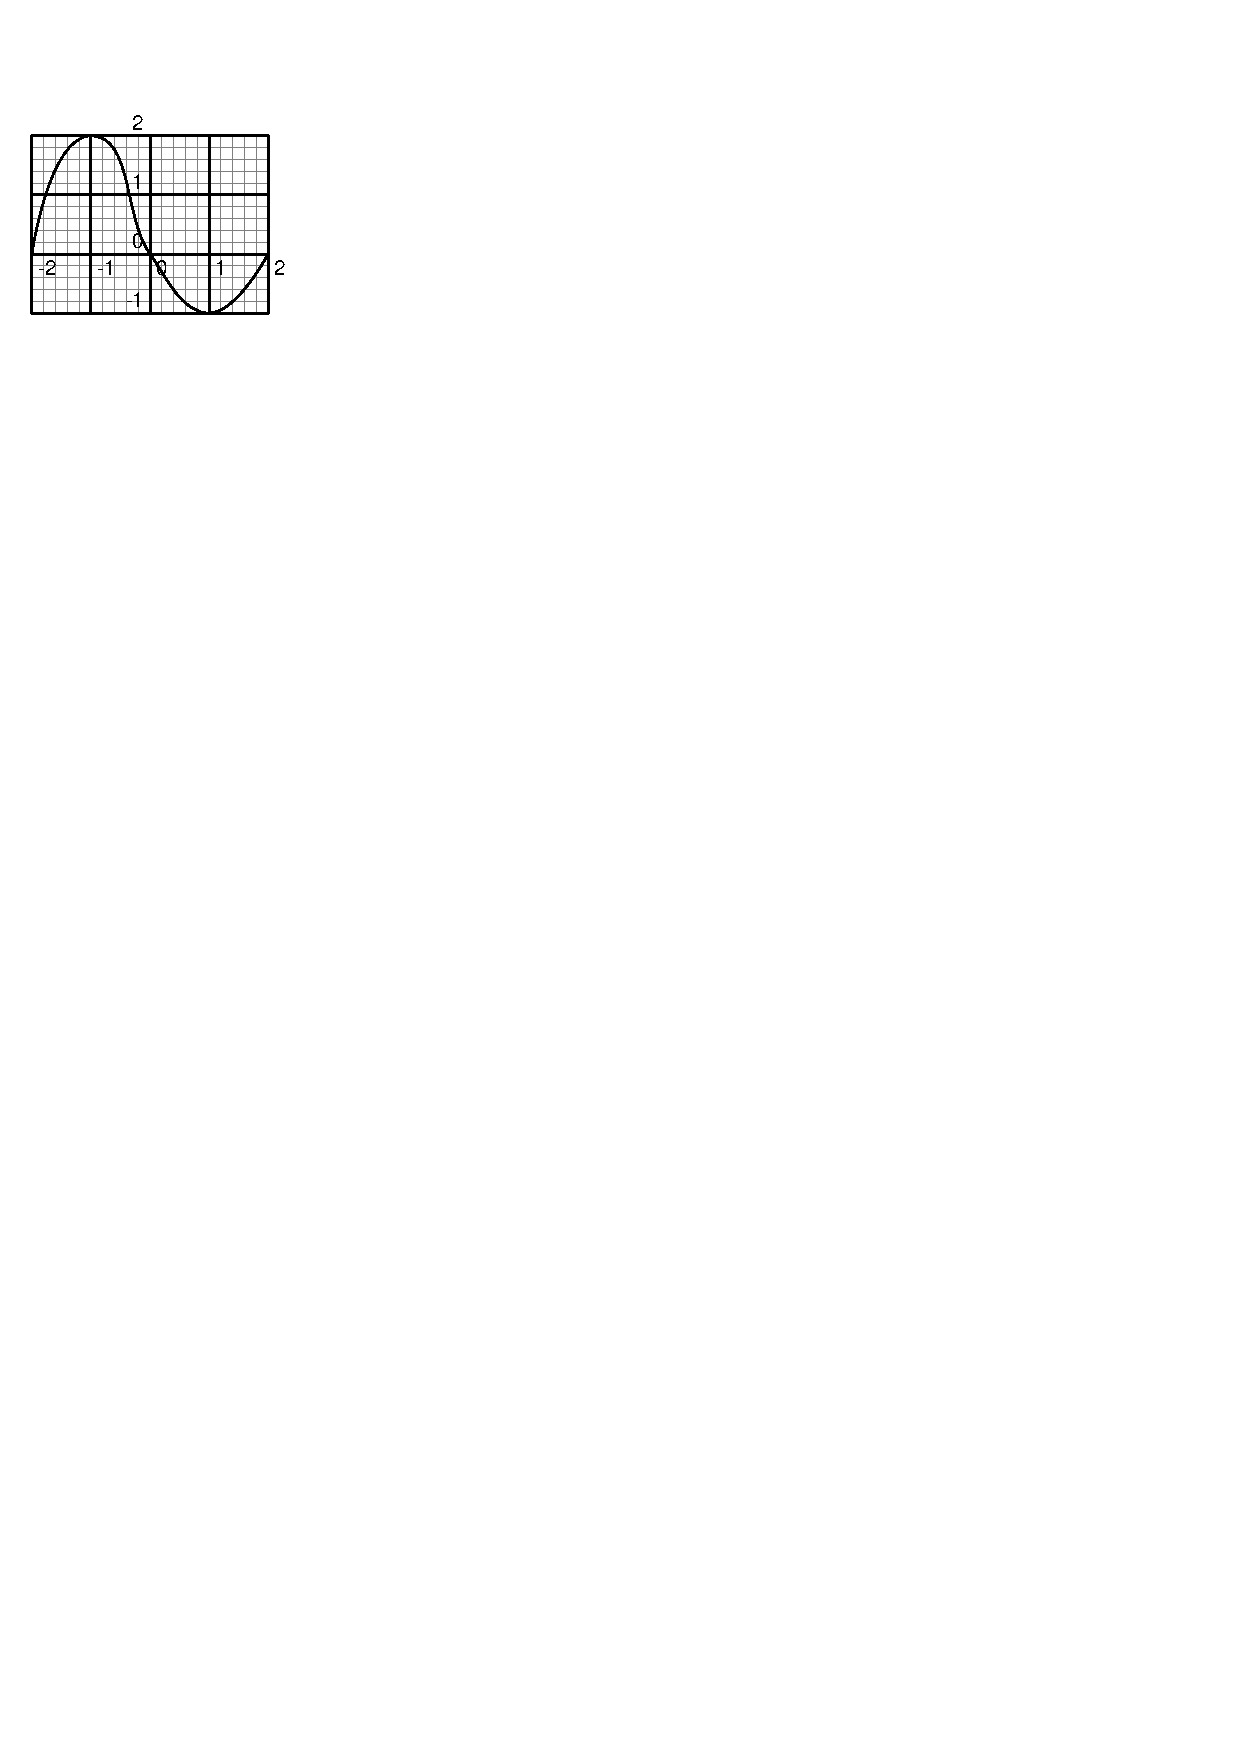
\includegraphics[bb=0 0 124 98,clip]{images/vector}
%%\end{wrapfigure}
%%��Ȥ���\Person{Donald}{Arseneau}�ˤ��\Sty{wrapfig}
%%��Ȥ��������������������Τ褦�ʽ��Ϥ����뤿���
%%\begin{InTeX}
%% \begin{wrapfigure}[5]{r}{5cm}
%% \includegraphics{file}
%% \end{wrapfigure}
%%\end{InTeX}
%%�Ȥ������Ϥ򤷤ޤ���
%




%\begin{Syntax}
% \C{DeclareGraphicsExtensions}\pa{��ĥ�ҤΥꥹ��}\\
% \C{DecrelaGraphicsRule}\pa{��ĥ��}\pa{����}\pa{�ɤ߹���ե�����}\pa{��
% �ޥ��}
%\end{Syntax}

%\subsection{EPS�ʳ��β�����ĥ�����}
%{\LaTeX}�Ǥ�EPS�ʳ��β�����ĥ����ߤ��ǽ
%�Ǥ��������ʤ�����ޤ������긵�ˤ�GIF��BMP��
%JPEG�ʤɤΥӥåȥޥåײ���������Ȼפ��ޤ���
%�ӥåȥޥåײ�����EPS���Ѵ��Ǥ���ġ����
%̵���Ǥ������󤢤ꡤͭ̾�ʤΤ�\prog{\IM}
%�Ǥ���{Windows}���ѤǤ���\Prog[EPSconv]{\EPSconv}\footnote{\webEpsconv}
%�Ȥ������եȥ�������Ƴ�����뤳�Ȥˤ�ꡤ
%��¸����ۤȤ�ɤβ�����EPS���Ѵ���ǽ�Ǥ���
%�����Υ��ץꥱ�������Ϥ����ޤǥӥåȥޥå�
%��EPS��������¸��������ʤΤǥե����륵��������
%����礭���ʤ�ޤ���
%
%�ǥХ����ɥ饤�ФȤ���\prog{\Dvipdfmx}��Ȥ���
%EPS�����ʳ��β����Ǥ�����ळ�Ȥ��Ǥ��ޤ���
%%����ʤ��BMP��JPG������{\EPSconv}��{\IM}�ʤɤ�
%%�ġ����Ȥäư���EPS���Ѵ������礬ɬ�פǤ���
%%��\prog{\Dvipdfmx}�ξ��Ϥ��μ�礬ɬ�פ���ޤ���
%�Ѵ����ʤ��Ƥ������������PDF��JPEG��PNG��MetaPost��4����
%�Ǥ���{Windows}��BMP�ʤɤ��㰵�̤�JPEG�ʤɤ�
%�Ѵ����ޤ���\fl{image.png} �����ä����
%ü���ʤɤ�
%\begin{InTerm}
%   \type{ebb image.png}
%\end{InTerm}
%�Ȥ����\fl{image.png}�Ѥ�\fl{image.bb}��
%��������ޤ���\prog{ebb}��{dvipdfm}��
%Ʊ������Ƥ��ޤ�������\texttt{image.bb}��
%�����ե�����νIJ�����������������Υ�
%������Ǥ���\texttt{image.bb} �򸫤��
%ʬ����ޤ�������Ȥ�
%\begin{InText}
%%%Title: ./image.png
%%%Creator: ebb Version 0.5.2
%%%BoundingBox: 0 0 595 841
%\end{InText}
%�ȤʤäƤ��ޤ��� \qu{\str{BoundingBox}}�Ȥ�
%������ɸ�Ȳ����νIJ���Ĺ�����ͤǤ���
%���˥������ե������ʲ��Τ褦�ˤ��ޤ���
%\begin{InTeX}
%\documentclass{jsarticle}
%\usepackage[dvipdfm]{graphicx}
%\begin{document}
%\includegraphics[width=3cm]{image.png}
%\end{document}
%\end{InTeX}
%��Ϥ��Ĥ��̤�˥����ץ��åȤ���DVI�ե������
%������\prog{\Dvipdfmx}��PDF�����������ɤ���
%�Ȥˤʤ�ޤ���
%
%\subsection{EPS����PDF�ؤ��Ѵ�}
%�ǥХ����ɥ饤�ФȤ���\prog{\Dvipdfmx}�Ǽ������
%EPS�����������褦�ˤ��Ƥ����硤\prog{\Dvipdfmx}
%��¹Ԥ��뤿�Ӥ����\Prog[Ghostscript]{\GS}��Ȥä�EPS����PDF���Ѵ�
%����������Ԥ��ޤ����������֤�û�̤Τ���ˡ�
%���餫����PDF���Ѵ����Ƥ������ɤ��Ǥ��礦��EPS����
%�β�����PDF���Ѵ�������ˡ�Ϥ����Ĥ����뤽���Ǥ�����
%��ñ�ǰ�������ˡ��Ҳ𤷤ޤ����ޤ�\prog{\GS}��
%\qu{pdfwrite}���Ϥ�ڤ����ˡ�Ǥ���BoundingBox��
%���ꤵ��Ƥ���EPS������\Prog{epstopdf}�ˤ�ä�
%PDF���Ѵ����ޤ���
%\begin{InTerm}
%   \type{epstopdf filename.eps}
%\end{InTerm}
%�Ȥ����\fl{filename.pdf}����������ޤ������ܸ줬
%�Ȥ��Ƥ���EPS�����ޤ������Ǥ��ʤ��ʤɤ�
%���꤬���뤫�⤷��ޤ��󡥤��ξ���GNU��
%\Prog[GhostScript]{\GS}�ΥС������7.07��Ȥ����ɤ���
%���礦���ʲ��Τ褦�ʥ����륹����ץ�\fl{epspdf}
%\begin{InText}
%#!/bin/bash
%FILE=$1
%fig=`basename $FILE .eps`
%epstopdf $FILE
%egrep "%%BoundingBox:" $FILE > $fig.bb
%\end{InText}
%�������\fl{/usr/local/bin/}�ʤɤ�ʣ������%$
%\begin{InTerm}
%   \type{epspdf filename.eps}
%\end{InTerm}
%�Ȥ����PDF�ե�����\fl{filename.pdf}�ȥХ����\indindz{�ե�����}{PDF}%
%���󥰥ܥå�������\fl{filename.bb}�����������
%����%\prog{echo}��ü����ʸ������Ϥ���̿�ᡤ
%%\prog{test}��ʸ����򸡺�����̿�ᡤ
%%\prog{egrep}�ϥե�����ʤɤ��������ɽ���򸫤Ĥ���̿�ᡤ
%%\prog{basename}�ϥե�����̾�����ĥ�Ҥ���������ꤹ��̿�ᡥ
%Ʊ���ǥ��쥯�ȥ��������Ƥ�EPS������
%PDF���Ѵ��������Ȥ���
%\begin{InText}
%#!/bin/sh
%for f in `ls *.eps`; do
%   fig=`basename $f .eps`
%   epstopdf $f
%   grep "^%%BoundingBox:" $f > $fig.bb
%done
%\end{InText}
%��\fl{epspdfs}�Ȥ���̾����Ʊ���褦��ʣ�����ޤ���
%���Τ褦�ˤ��ƽ�������PDF��{\LaTeX}�θ��Ƥ�
%\begin{InTeX}
%\documentclass{jsarticle} 
%\usepackage[dvipdfm]{graphicx}
%\begin{document}
%\includegraphics{filename.pdf}
%\end{document}
%\end{InTeX}
%�Τ褦�ˤ��Ƽ����ळ�Ȥ��Ǥ��ޤ���
%
%\begin{comment}
%���ʤߤ�\fl{filename.bb}��
%\begin{InText}
%%%Title: filename.dvi
%%%Creator: hoge
%%%BoundingBox: 142 160 443 665
%%%CreationDate: Tue Dec 30 16:01:48 2003
%\end{InText}
%�Τ褦�ʾ��󤬽��Ϥ���Ƥ���Ǥ��礦���������
%\begin{InText}
%%%BoundingBox: 142 160 443 665 
%\end{InText}
%�Ȥ���1�Ԥ�������С�\prog{\Dvipdfmx}���ϲ�����
%ĥ����ळ�Ȥ��Ǥ��ޤ���
%%%�ʾ�Τ褦�ʥ����륹����ץȤ�ư����뤳�Ȥ��Ǥ��ʤ�Windows�桼����
%%%���ϥե꡼��Cygwin��Ƴ�������Τ��ɤ��Ȼפ��ΤǤ���\verb|^^;|��
%\end{comment}

\section{�������ˡ}
{\LaTeX}�ǿޤ��갷�����ʤϤ����Ĥ�¸�ߤ��ޤ���
�̿��Τ褦�ʲ�����\sty{graphicx}�ѥå�����
�ʤɤ�Ȥä�ĥ�������ˡ�ȡ�1�������褹����ˡ�Ǥ���
\sty{graphicx}�ѥå��������Ѥ��ƴ�¸�β�����ĥ�����
��ˡ��\secref{figure}�򻲾Ȥ��Ƥ���������������
�ޤ��������Ƥ��ʤ��ʳ��Ǥ��������ˡ��Ҳ𤷤ޤ���

�������ˡ���礭��ʬ������Ĥ���ޤ�����Ĥ�{\LaTeX}
���Ȥ�ǽ�Ϥ����褹����ˡ�� \cmd{special}̿���Ȥ�
¾�Υץ������ʥǥХ����ɥ饤�����ˤ���������ͤ���ˡ�Ǥ������̤�
{\LaTeX}�ˤ����������ǽ�Ϥ�{\TeX}����Υ����ƥ��
�������ϼ�ʤ�ΤȤʤäƤ��ޤ�����ñ�ʿޤ��������
�ʤ��{\LaTeX}������äƤ���\env{picture}�Ķ���
��������Ԥ��Τ���ڤǤ���

\subsection{�٤��񤭤ˤ��ޤκ���}
��äȤ��ñ���������ˡ�Ȥ���{\LaTeX}�Ǥ٤��񤭤�
�Ԥ���\Env{verbatim}�Ķ���Ȥ������ͤ����ޤ���
\env{verbatim}�Ķ���Ǥ�ʸ����{\KY{����}}�˶ᤤ���ͤ��
�Ȥޤ��Τǡ����Ƥ����Ϥ��Ƥ���ɽ����DVI�ե�����
�ؤν��Ϥ�Ʊ���褦�ˤʤ�ޤ�%
\footnote{\Hito{����}{����}�κ�������\Prog{plain2}�Ȥ����ġ����Ȥ�����
�ѵ�����Ȥ߹�碌����ˤ�ä�{\LaTeX}�Ѥο�ɽ��������뤳�Ȥ�Ǥ��ޤ���}��

\begin{Exe}
�ʲ�����������򻲹ͤˤ٤��񤭤ˤ���ޤ򤷤ƤߤƤ���������
\begin{InOut}
\begin{verbatim}
       a
      /  \
     /    \
    b      c
   / \    / \
  d   e  f   g
\end{verbatim}
\end{InOut}

%\env{verbatim}�Ķ���Ǥ�Ⱦ�Ѥζ����Ȥ鷺��
%���Ѥζ����Ȥ����ɤ��Ǥ��礦��Ⱦ�Ѥζ����
%�ƥ����ȥ��ǥ��å������Ϥ��Ƥ���ʬ�ζ���
%���������櫓�ǤϤ���ޤ���
\end{Exe}




\subsection{��
  ��������}
\indindz{����}{���ץ饤��}\indindz{����}{���}\indindz{����}{�٥���}%
{\KY{�٥��ȥ����}}�ʤɤǤ�{\KY{�٥�������}}
�Ȥ�{\KY{���ץ饤�����}}�Ȥ���{\KY{�������}}
���Ȥ��Ƥ����¿���λ��ͽ�ǵ��Ҥ���Ƥ��ޤ����٥��ȥ������
�Τ뤦���ǥ٥��������θ������ΤäƤ����ȡ�������������
����Ƭ����Ƕ����򥤥᡼�����䤹���Ȼפ��ޤ��ΤǾҲ�
���Ƥ����ޤ�����餫�ʶ�������������ˤ�¿��������ɸ
��ɬ�פˤʤ�Ȼפ��ͤ⤤��Ǥ��礦�����������ٳ�餫
�ʶ�������������ˤ�3������н�ʬ�Ǥ���\indindz{��}{����}
�����������������\pp{\Z{������}}�����ʤ���о��ʤ��ۤɾ���
�̤Ͼ��ʤ��ʤ�Τǡ����ʤ��������dz�餫�ʶ���������
��ˡ�������Ϻ�����ޤ�����������Ǥ�٥��������Ϲ�
����Ĥδ�����Ȱ�Ĥ�������\pp{$2+1$��}������и��߻�
������\prog{Illustrator}�ʤɤǤ褯������������ˤʤ�
�ޤ������θ�����\Prog{Illustrator}�Υڥ�ġ���˳褫
����Ƥ��ޤ��Τǡ������������ϳ�ǧ���Ƥ����������ɤ���
���礦������\Prog{Illustrator}�ξ��ϥ桼���θ�����
���ս���͡��ʹ��פ��ʤ���Ƥ��ޤ���

��������������ˤ���$n$�Ĥ������������ꤽ��$i$����
�κ�ɸ��$P_i=(x_i,y_i)$�Ȥ���\equref{bez1}��
\equref{bez2}��ɽ��������٥��������ȸƤӤޤ���
\begin{eqnarray}
P(u)&=&\sum^{n-1}_{i=0} P_i\, B_{i, n} (u)\equlab{bez1}\\
B(u)&=&\frac{n!}{i!\, (n-i)!}u^i(1-u)^{n-i}\equlab{bez2}
\end{eqnarray}
\indindz{�ե����}{Type1}%%
���줬�٥��������ΰ��̷��Ǥ�������Ȥ���Type1�ե���Ȥ�
��Ȥ��Ƥ��롩2���٥��������򼨤��ޤ���
ʿ�̺�ɸ��$P_0=(-1,1)$��$P_1=(0,0)$��$P_2=(1,1)$��
����Ȥ����\equref{bez1}��\equref{bez2}��ꡤ
\begin{eqnarray}
 P(u)&=& P_0 B_{0,2} + P_1 B_{1,2} + P_1 B_{1,2} \nonumber\\
     &=& P_0 (1-u)^2 + P_12u(1-u) + P_2 u^2 \equlab{bez3}
\end{eqnarray}
�Ȥʤ�\equref{bez3}���Ф���̵����$u$��Ϳ��
��г�餫�ʶ����������ޤ��������3�����Ǥ�Ʊ
�ͤ˷׻��Ǥ���Τ������ʼ��Ǥ�����δ��������������
�٥���������\figref{bez1}���̤�ˤʤ�ޤ���
\begin{figure}[htbp]
\begin{center}
\setlength{\unitlength}{1cm}
\begin{picture}(6,4)(0,0)
 \put(0,2){\vector(1,0){6}}
 \put(6.2,2){\makebox(0,0)[b]{$x$}}
 \put(3,0){\vector(0,1){4}}
 \put(3.2,4){\makebox(0,0)[t]{$y$}}
 \multiput(0,1.9)(1,0){6}{\line(0,1){.2}}
 \multiput(2.9,0)(0,1){4}{\line(1,0){.2}}
 \put(2,3){\circle{.1}}
 \put(2,3.1){\makebox(0,0)[b]{$P_0$}}
 \dashline{.1}(2,3)(3,2)
 \put(3,2){\circle{.1}}
 \put(2.8,1.9){\makebox(0,0)[t]{$P_1$}}
 \put(3.2,1.9){\makebox(0,0)[t]{$O$}}
 \put(4,3){\circle{.1}}
 \put(4,3.1){\makebox(0,0)[b]{$P_2$}}
 \dashline{.1}(4,3)(3,2)
 \qbezier(2,3)(3,2)(4,3)
\end{picture}
\caption{�������ȼ�����������٥�������}\figlab{bez1}
\end{center}
\end{figure}
���Τ褦�ʸ������ΤäƤ����ȸ�ۤɾҲ𤹤�
{\LaTeX}��\env{picture}�Ķ��ǻ��ѤǤ���̿���
�������Ω�Ļ��Ǥ��礦��������{\LaTeX}
�Ǥ�¿���Υ٥����������������ޥ�ɤϤ�ä�
�׻��ξ��ʤ����르�ꥺ���ȤäƤ����礬
����ޤ������ǥХ����ɥ饤�Ф������Ǥ���Ƥ���
���⤢��ޤ���


\subsection{\env{picture}�Ķ��ˤ������}
{\LaTeX}���Ϥ�Ȥä������Ԥ��ˤ����̤ʴĶ���
�������Ѥ�\Env{picture}�Ķ��Ǻ�Ȥ�Ȥ��ޤ���
\env{picture}�Ķ��Ǥϴ��Ȥʤ�Ĺ������Ƥ���
����Ū�ʵ�Υ�ˤ�ä������Ԥ��ޤ������ΤȤ����
�Ȥʤ�Ĺ�� \cmd{unitlength}����ޤ���
\begin{Syntax}
\verb+\begin{picture}+\xy{x}{y}\xy{$x_0$}{$y_0$}\\
\va{��������}\\
\verb+\end{picture}+
\end{Syntax}
\env{picture}�Ķ���������褷�������Ƥ�
���Ҥ��ޤ���\env{picture}�Ķ����Ϥ�\qu{\xy{x}{y}}
��ɬ�ܰ����Ǥ���\qu{\xy{$x_0$}{$y_0$}}��Ǥ�հ����Ǥ���
\qu{\xy{x}{y}}�ˤϺ�ɸ�ˤ�����\env{picture}�Ķ����礭��
��������$x$�ǽ�������$y$�ǻ��ꤷ�ޤ���
����ˤ�ñ�̤ʤɤ��դ����˿��ͤǻ��ꤷ�ޤ���
\qu{\xy{$x_0$}{$y_0$}}�ˤϸ����ΰ��֤���ꤷ�ޤ���

���餫�����Ǥ����֤���ˤ� \cmd{put}�� \cmd{multiput}��
�Ȥ��ޤ���$x$��$y$��ñ�� \cmd{unitlength}��
��°���ޤ���
\begin{Syntax}
\Cmd{put}\xy{x}{y}\pa{����}\\
\Cmd{multiput}\xy{x}{y}\xy{$\Delta{x}$}{$\Delta{y}$}%
  \pa{���}\pa{����}
\end{Syntax}
\cmd{put}̿��Ϻ�ɸ\xy{x}{y}��\va{����}���֤�������
̿��Ǥ���\cmd{multiput}�Ϻ�ɸ\xy{x}{y}������Ȥ���
����ܤκ�ɸ\xy{$\Delta{x}$}{$\Delta{y}$}��\Z{�٥��ȥ�}
�Ȥ���\xy{$\Delta x$}{$\Delta y$}���Ѳ��̤˱�����
���Ǥ���ʬ���������֤������֤��ޤ���
����¾��2���٥������������� \Cmd{qbezier}̿�᤬����ޤ���\zindind{����}{������}
\begin{Syntax}
\Cmd{qbezier}\xy{$x_1$}{$y_1$}\xy{$x_2$}{$y_2$}\xy{$x_3$}{$y_3$}
\end{Syntax}
\qu{\xy{$x_1$}{$y_1$}}�������\qu{\xy{$x_2$}{$y_2$}}
��������\qu{\xy{$x_3$}{$y_3$}}�����Ȥ���2���٥���
�����������ޤ���

\va{����}�ˤϼ��Τ褦�ʥ��ޥ�ɤ�ɸ��Ȥ��ƻȤ��ޤ���
\begin{Syntax}
\Cmd{line}\xy{x}{y}\pa{��}\\
\Cmd{vector}\xy{x}{y}\pa{��}\\
\Cmd{circle*}\pa{ľ��}\\
\Cmd{oval}\xy{��}{�⤵}\opa{���ֻ���}
\end{Syntax}
\cmd{line}��\qu{\xy{x}{y}}��٥��ȥ�Ȥ���
\va{Ĺ��}ʬ����ʬ�������ޤ���\cmd{vector}�� \cmd{line}
�ν�ü��\Z{���}��Ĥ�����ΤǤ���
\cmd{circle*}��ľ�¤���ꤷ��\Z{��}�������ޤ���\indindz{����}{�ߤ�}%
�������ꥹ��\qu{\texttt*}���դ��ʤ��ȱߤ���¦���ɤ�Ĥ֤���ޤ���
\cmd{oval}�����ȹ⤵����ꤷ���ʱߤ������ޤ���\indindz{����}{�ʱߤ�}%
\begin{InOut}
\setlength{\unitlength}{1mm}
\begin{picture}(40,30)
\put(10,10){\line(1,1){10}}
\put(10,0){\vector(1,1){10}}
\put(20,20){\circle{5}}
\end{picture} 
\end{InOut}
�ʱߤ����� \cmd{oval}̿���Ǥ�հ�����\va{���ֻ���}
�ˤ��ʱߤΤɤ���ʬ����Ϥ��뤫����ꤷ�ޤ���
���줾�����\qu{\str t}������\qu{\str b}��
��\qu{\str l}����\qu{\str r}�Ȥʤꡤʣ��Ū��
���ѤǤ��ޤ���
\begin{InOut}
\setlength{\unitlength}{1mm}
\begin{picture}(50,30)
\put(8,12){\oval(10,15)[tl]}
\put(8,8){\oval(10,15)[bl]}
\put(10,10){\oval(10,15)}
\put(12,12){\oval(10,15)[tr]}
\put(12,8){\oval(10,15)[br]}
\end{picture} 
\end{InOut}
\env{picture}�Ķ���Ǥ�����������
\Cmd{thinlines}�� \Cmd{thicklines}����Ĥ�Ĵ��
���ޤ���\cmd{thinilnes}�Τۤ����٤� \cmd{thicklines}
�Τۤ��������ʤ�ޤ���\env{picture}�Ķ��������
����ʬ��ͭ���ˤʤ�ޤ���
\begin{InOut}
\setlength{\unitlength}{1mm}
\begin{picture}(50,30)
\thicklines
\put(10,10){\line(1,1){10}}
\put(10,20){\vector(1,1){10}}
\thinlines
\put(10,0){\vector(1,1){10}}
\put(20,20){\circle{5}}
\end{picture}  
\end{InOut}

\begin{Exe}
\figref{bez1}�� \env{picture} �Ķ������褹��ˤϤɤ������
�ɤ�����ͤ��Ƥ�����������򼨤��Ȱʲ��Τ褦�ʵ��Ҥˤʤ�ޤ���

\C*{makebox}%
\begin{InTeX}
\setlength{\unitlength}{1cm}
\begin{picture}(6,4)(0,0)
 \put(0,2){\vector(1,0){6}}
 \put(6.2,2){\makebox(0,0)[b]{$x$}}
 \put(3,0){\vector(0,1){4}}
 \put(3.2,4){\makebox(0,0)[t]{$y$}}
 \multiput(0,1.9)(1,0){6}{\line(0,1){.2}}%���
 \multiput(2.9,0)(0,1){4}{\line(1,0){.2}}%���
 \put(2,3){\circle*{.1}}
 \put(2,3.1){\makebox(0,0)[b]{$P_0$}}
 \dashline{.1}(2,3)(3,2)%���
 \put(3,2){\circle*{.1}}
 \put(2.8,1.9){\makebox(0,0)[t]{$P_1$}}
 \put(3.2,1.9){\makebox(0,0)[t]{$O$}}
 \put(4,3){\circle*{.1}}
 \put(4,3.1){\makebox(0,0)[b]{$P_2$}}
 \dashline{.1}(4,3)(3,2)%���
 \qbezier(2,3)(3,2)(4,3)
\end{picture}
\end{InTeX}

\end{Exe}

\subsection{\env{picture}�Ķ��γ�ĥ����1\zdash \sty{epic}}
{\LaTeX}�Ǥ�ɸ���\env{picture}�Ķ��Υ��ޥ�ɤ�
�ǥХ����˰�¸���ʤ��Τ�������������ΤǤ�����
����ǤϤ��ޤ�ˤ�ɽ���Ϥ�˳�����Τ������Ǥ���
�����Ǥ���\env{picture}�Ķ��γ�ĥ���Ԥ���
���ޤ�����\env{picture}�Ķ��˸¤餺{\LaTeX}�Ǥ�����
��1980ǯ���Ⱦ���餵�ޤ��ޤ���ˡ���Ϻ����졤��ĥ
����³���ޤ�����������Ǥ�\Person{Sunil}{Podar}�ˤ��
\Sty{epic}��\env{picture}�Ķ��γ�ĥ�ǤȤ��Ƥ���ɾ��
����ޤ���\sty{epic}�Ǥ�{\LaTeX}��\env{picture}�Ķ�
�ǻ��ѤǤ��륳�ޥ�ɤΤۤ��˰ʲ���̿�᤬��ĥ����Ƥ��ޤ���
\begin{quote}% underfull
\begin{tabular}{lllll}
\Cmd{multiputlist}&\Cmd{matrixput}&\Cmd{grid}&\Cmd{picsquare}&\Cmd{dottedline}\\
\Cmd{dashline}&\Cmd{drawline}&\Cmd{jput}&\Cmd{putfile}& \\
\end{tabular}


\end{quote}
���Τۤ���\Env{dottedjoin}��\Env{dashjoin}��\Env{drawjoin}��
���ĤδĶ����������Ƥ��ޤ���
��ɸ���Ѳ��̤�\xy{$\Delta{x}$}{$\Delta{y}$}�Ȥ���ʣ����
���ܤ����֤��� \cmd{multiputlist}̿�᤬����ޤ���
\begin{Syntax}
\Cmd{multiputlist}\xy{x}{y}\xy{$\Delta{x}$}{$\Delta{y}$}%
   \opa{tbrl}\pa{ʣ���ι���}
\end{Syntax}
% tbrl �Τ����줫����ꤷ�ޤ���
��ɸ��˹���Τ褦�����Ǥ򷫤��֤������֤��� \cmd{matrixput}̿��⤢��ޤ���
\begin{Syntax}
\Cmd{matrixput}\xy{x}{y}\xy{$\Delta{x_1}$}{$\Delta{y_1}$}%
   \pa{$n_1$}\xy{$\Delta{x_2}$}{$\Delta{y_2}$}%
   \pa{$n_2$}\pa{����}
\end{Syntax}
\begin{InOut}
\setlength{\unitlength}{1pt}
\begin{picture}(150,110)(0,0)
\multiputlist(0,0)(15,10)%
  {0,1,2,3,4,5,6,7,8,9,10}
\matrixput(0,0)(20,0){7}(0,20)%
   {5}{\mbox{̤��}}
\end{picture} 
\end{InOut}
��ɸ�Ϥ�ɽ������Τ˳ʻҤ������ˤ� \cmd{grid}̿�᤬�Ȥ��ޤ���
\begin{Syntax}
\Cmd{grid}\xy{��}{�⤵}\xy{$\Delta{\text{��}}$}{$\Delta{\text{�⤵}}$}%
   \opa{$x$��ɸ�ν����,$y$��ɸ�ν����}
\end{Syntax}
%\begin{InOut}
%\begin{picture}(150,100)(0,0)
%\put(10,10){\grid(50,50)(10,10)[0,0]}
%\end{picture} 
%\end{InOut}
\indindz{����}{�ޤ�����}\indindz{����}{������}\indindz{����}{������}%%
¾�ˤ������������ʤɤ��������ޥ�ɤ�����ޤ���
\begin{Syntax}
\Cmd{dottedline}\opa{���μ���}\pa{�ֳ�}%
   \xy{$x_1$}{$y_1$}\xy{$x_2$}{$y_2$}$\cdots$\xy{$x_n$}{$y_n$}\\
\Cmd{dashline}\pa{������Ĺ��}\opa{�ֳ�}%
   \xy{$x_1$}{$y_1$}\xy{$x_2$}{$y_2$}$\cdots$\xy{$x_n$}{$y_n$}\\
\Cmd{drawline}\xy{$x_1$}{$y_1$}\xy{$x_2$}{$y_2$}$\cdots$\xy{$x_n$}{$y_n$}
\end{Syntax}
\cmd{dottedline}��������\cmd{dashline}��������
\cmd{drawline}��\Z{�ޤ���}����������˻Ȥ��ޤ���\Z{����}��\Z{����}��
�ޤ�Ƥ⹽���ޤ���
\begin{InOut}
\setlength{\unitlength}{1pt}
\begin{picture}(150,120)(0,0)
\put(0,0){%
  \grid(100,100)(25,25)[0,0]}
\dottedline[$\circ$]{10}(0,0)
  (100,100)
\dashline{3}(0,80)(30,50)(50,45)
  (100,20)
\drawline(0,70)(10,60)(30,40)
  (100,50)
\end{picture} 
\end{InOut}

\subsection{\env{picture}�Ķ��γ�ĥ����2\zdash \sty{eepic}}
\Person{Sunil}{Podar}�ˤ��\Sty{epic}����ɡ���ĥ������ΤȤ��ơ�
\Person{Conrad}{Kwok}�κ�������\Sty{eepic}������ޤ��������\sty{epic}��
���ɡ���ĥ�ǤǤ���ޤ��Τǻ��Ѥ���Ȥ��ϼ��Τ褦��\sty{epic}������ɤ߹�
��Ǥ����ޤ���

\begin{InTeX}
\usepackage{epic,eepic} 
\end{InTeX}

{\LaTeX}��\env{picture}�Ķ��ǻ��ѤǤ��� \cmd{line}��
\cmd{circle*}��\cmd{oval}�γ�ĥ���Ԥ��Ƥ��ޤ���
\sty{epic}�Υ��ޥ�ɤ����ƺ��������Ƥ��ޤ���
\sty{eepic}�Ϥ�����̿���{\Tpic}���ڥ������֤�����
�Ƥ��ޤ��Τ������ϤϹ⤤�ΤǤ������ǥХ����ɥ饤�Ф�
{\Tpic}���ڥ������б����Ƥ���ɬ�פ�����ޤ���
\prog{dviout}��\prog{dvips}��\prog{\Dvipdfmx}�ʤɤ�
�б����Ƥ���褦�Ǥ����ǥХ����ɥ饤�Фˤ�ä�{\Tpic} 
���ڥ����β�᤬�㴳�ۤʤ�褦�Ǥ��Τǡ����Ϥ��ǧ����
�ǥХ��������򤷤Ƥ���������

���������˴ؤ��륳�ޥ�ɤ��������������Ƥ��ޤ���
\begin{Syntax}
\Cmd{allinethickness}\pa{����} \\
\Cmd{Thicklines}
\end{Syntax}
\cmd{allinethickness}�Ϥ���̿���Ȥä����
\env{picture}�Ķ���ˤ������Ƥ������������ѹ����ޤ���
\Cmd{Thicklines}�� \Cmd{thicklines}���⤳�Υ��ޥ�ɤ�
���������������������������ޤ���
\setlength\unitlength{1pt}
\begin{InOut}
\begin{picture}(100,100)(0,0)
\newcommand\VP[2]{%
  \put(0,0){\vector(#1,#2){70}}}
\thinlines  \VP{1}{0}
\thicklines \VP{1}{1} \VP{0}{1}
\Thicklines \VP{2}{1}
\end{picture} 
\end{InOut}
\sty{eepic}�Ǥ� \cmd{drawline}���� \C{path}��Ȥ���
\C{qbezier}���� \C{spline}��Ȥ����ɤ��Ǥ��礦��
\C{spline}�ϻ����Ƚ����ʳ����������Ȥ���
\Z{Chaikin����}�������ޤ���\indindz{����}{Chaikin}
\begin{Syntax}
\Cmd{path}\xy{$x_1$}{$y_1$}\xy{$x_2$}{$y_2$}%
   $\cdots$\xy{$x_n$}{$y_n$}\\
\Cmd{spline}\xy{$x_1$}{$y_1$}\xy{$x_2$}{$y_2$}%
   $\cdots$\xy{$x_n$}{$y_n$}
\end{Syntax}
\begin{InOut}
\setlength{\unitlength}{1pt}
\begin{picture}(150,100)(0,0)
\path(0,60)(25,100)(100,25)
 (150,50)(100,100)(25,0)(55,75)
\Thicklines
\spline(0,60)(25,100)(100,25)
 (150,50)(100,100)(25,0)(55,75)
\end{picture} 
\end{InOut}
������ʱߤ������Τ� \cmd{ellipse}��\index{��}\index{�߸�}%
�̤������ˤ� \cmd{arc}��Ȥ��ޤ���
�������ꥹ�����դ�����ΰ���ɤ�Ĥ֤��ޤ���
\begin{Syntax}
\Cmd{ellipse*}\pa{��}\pa{�⤵}\\
\Cmd{arc}\pa{��}\pa{��������}\pa{��������}
\end{Syntax}
\va{��������}���ͤ�$[0,\pi/2]$���ϰϤˡ�
\va{��������}���ͤ�$[\text{��������},\text{��������}+2\pi]$
���ϰϤˤ��ޤ����ΰ���ɤ�Ĥ֤��ˤ� \C{filltype} ��Ȥ��ޤ���
�������ꥹ�����դ������� \Cmd{circle*}
�� \Cmd{ellipse*}���ΰ���ɤ�Ĥ֤������\qu{\str{black}}��
\qu{\str{white}}��\qu{\str{shade}}�λ��Ĥ������򤷤ޤ���
\begin{Syntax}
\Cmd{filltype}\pa{����}
\end{Syntax}
%   \blacken        \whiten         \shade
%   \texture        \filltype{type} type=black|white|shade
\begin{InOut}
\begin{picture}(150,100)(0,0)
\filltype{shade}
\put(10,50){\ellipse*{50}{30}}
\filltype{black}
\put(50,50){\ellipse*{30}{50}}
\put(80,50){\ellipse{45}{65}}
\end{picture} 
\end{InOut}

\subsection{\env{picture}�Ķ��γ�ĥ����3\zdash \sty{pict2e}}
\person{Hubert}{G\"a\ss lein}��
\Person{Rolf}{Niepraschk}�ˤ��\Sty{pict2e}��
\Env{picture}�Ķ��γ�ĥ�Ȥ���2003ǯ���˸�ɽ
���줿��ΤǤ����ǥХ����ɥ饤�Ф��Ϥ�ڤ��
\env{picture}�Ķ��ǻ��ѤǤ��륳�ޥ�ɤ�����
���Ƥ��ޤ��������������ޥ�ɤ��������Ƥ��ޤ���
���ν�
\begin{quote}
 \str{dvips} \str{xdvi} \str{pdftex} \str{vtex} \str{dvipdfm}
\end{quote}
�ʤɤΥǥХ����ɥ饤�Ф򥵥ݡ��Ȥ��Ƥ��ޤ���
\env{picture}�Ķ��ˤ�����ۤȤ�ɤΥ��ޥ�ɤ�
��ĥ���Ƥ���ޤ���\cmd{circle}��������ߤ��礭���ˤ�\indindz{����}{�ߤ�}%
���¤Ϥ���ޤ��󡥥٥��������˴ؤ��Ƥ� \cmd{cbezier}̿��
���ɲä���ޤ�����
\begin{Syntax}
\Cmd{qbezier}\xy{$x_1$}{$y_1$}\xy{$x_2$}{$y_2$}\xy{$x_3$}{$x_3$}\\
\Cmd{cbezier}\xy{$x_1$}{$y_1$}\xy{$x_2$}{$y_2$}\xy{$x_3$}{$x_3$}\xy{$x_4$}{$x_4$}\\
\end{Syntax}
\cmd{qbezier}��\Z{2���٥�������}�ѡ�\cmd{cbezier}��\Z{3���٥���������}
��̿��Ǥ���\indindz{����}{2���٥���}\indindz{����}{3���٥���}%
\begin{InOut}
\setlength{\unitlength}{1pt}
\begin{picture}(100,100)(0,0)
\qbezier(0,0)(50,100)(100,0)
\cbezier(0,0)(25,200)
  (75,0)(100,100)
\end{picture}
\end{InOut}

\section{¾�Υץ������ˤ������}
�����Ȥ��Ƥ�������ġ����Ҳ𤷤ޤ���
�ʲ�������ġ���Ǻ��������ޤʤɤ�
���줾����ꤵ�줿��ˡ�ǥǥХ����ɥ饤�Ф�
Ŭ�ڤ˲��Ǥ�����֤ˤʤ���Фʤ�ޤ���


\subsection{\texorpdfstring{\Tpic}{Tpic}�ˤ������}

Unix��OS������ġ���Ȥ���\Person{Brian}{Kernighan}��
��ȯ����\Prog[PIC]{\PIC}������ޤ��������
\Person{Tim}{Morgan}��{\TeX}�˰ܿ�����\Prog[Tpic]{\Tpic}
��Ȥ��ȴ�ñ�ʿ޷��ʤ�Ф��������������Ǥ��ޤ���
Unix��OS����äƤ���ʤ��\prog{\PIC}�Ȥ����ץ�
����बƳ������Ƥ���Ǥ��礦������\prog{\PIC}��
���ܸ첽����Ƥ��ʤ����⤷��ʤ��Τ����դ��Ƥ���������
{\Tpic}�ϤۤȤ�ɤε�ǽ��{\TeX}�ǤϤʤ��ǥХ���
�ɥ饤�Ф�Ǥ���Ƥ��ޤ���������̿��� \cmd{special}
̿�����˵��Ҥ���Ƥ��ޤ���{\Tpic}�ν��Ϥ�����ͭ��
̿���{\Tpic}���ڥ����ȸ����ޤ���{\Tpic}���ڥ�����
�б����Ƥ���ɥ饤�Ф�\prog{dvips}��\prog{dviout}��
\prog{\Dvipdfmx}�ʤɤǤ���¿���Υɥ饤�Ф��б�
���Ƥ��ޤ������ǥХ����ɥ饤�Фˤ����ΰ㤤�ʤ�
�⤢��ޤ��ΤǼ㴳���դ�ɬ�פǤ��礦��

\begin{Exe}\label{exe:tpicsample}
�㤨��\figref{tpicsample}�Τ褦�ʿޤ�����������Ȥ��ޤ��礦��
\begin{figure}[htbp]
\begin{center}
 %\expandafter\ifx\csname graph\endcsname\relax \csname newbox\endcsname\graph\fi
\expandafter\ifx\csname graphtemp\endcsname\relax \csname newdimen\endcsname\graphtemp\fi
\setbox\graph=\vtop{\vskip 0pt\hbox{%
    \special{pn 8}%
    \special{pa 0 500}%
    \special{pa 750 500}%
    \special{pa 750 0}%
    \special{pa 0 0}%
    \special{pa 0 500}%
    \special{fp}%
    \graphtemp=.5ex\advance\graphtemp by 0.250in
    \rlap{\kern 0.375in\lower\graphtemp\hbox to 0pt{\hss PIC file\hss}}%
    \special{pa 750 250}%
    \special{pa 1250 250}%
    \special{fp}%
    \special{sh 1.000}%
    \special{pa 1150 225}%
    \special{pa 1250 250}%
    \special{pa 1150 275}%
    \special{pa 1150 225}%
    \special{fp}%
    \graphtemp=\baselineskip\multiply\graphtemp by -1\divide\graphtemp by 2
    \advance\graphtemp by .5ex\advance\graphtemp by 0.250in
    \rlap{\kern 1.000in\lower\graphtemp\hbox to 0pt{\hss pic\hss}}%
    \special{pa 1250 500}%
    \special{pa 2000 500}%
    \special{pa 2000 0}%
    \special{pa 1250 0}%
    \special{pa 1250 500}%
    \special{fp}%
    \graphtemp=.5ex\advance\graphtemp by 0.250in
    \rlap{\kern 1.625in\lower\graphtemp\hbox to 0pt{\hss \textsc{Tpic} file\hss}}%
    \special{pa 2000 250}%
    \special{pa 2500 250}%
    \special{da 0.050}%
    \special{sh 1.000}%
    \special{pa 2400 225}%
    \special{pa 2500 250}%
    \special{pa 2400 275}%
    \special{pa 2400 225}%
    \special{fp}%
    \graphtemp=\baselineskip\multiply\graphtemp by -1\divide\graphtemp by 2
    \advance\graphtemp by .5ex\advance\graphtemp by 0.250in
    \rlap{\kern 2.250in\lower\graphtemp\hbox to 0pt{\hss input\hss}}%
    \special{pa 2500 500}%
    \special{pa 3250 500}%
    \special{pa 3250 0}%
    \special{pa 2500 0}%
    \special{pa 2500 500}%
    \special{fp}%
    \graphtemp=.5ex\advance\graphtemp by 0.250in
    \rlap{\kern 2.875in\lower\graphtemp\hbox to 0pt{\hss {\LaTeX} file\hss}}%
    \special{pa 3250 250}%
    \special{pa 3750 250}%
    \special{fp}%
    \special{sh 1.000}%
    \special{pa 3650 225}%
    \special{pa 3750 250}%
    \special{pa 3650 275}%
    \special{pa 3650 225}%
    \special{fp}%
    \graphtemp=\baselineskip\multiply\graphtemp by -1\divide\graphtemp by 2
    \advance\graphtemp by .5ex\advance\graphtemp by 0.250in
    \rlap{\kern 3.500in\lower\graphtemp\hbox to 0pt{\hss {\LaTeX}\hss}}%
    \special{pa 3750 500}%
    \special{pa 4500 500}%
    \special{pa 4500 0}%
    \special{pa 3750 0}%
    \special{pa 3750 500}%
    \special{fp}%
    \graphtemp=.5ex\advance\graphtemp by 0.250in
    \rlap{\kern 4.125in\lower\graphtemp\hbox to 0pt{\hss DVI\hss}}%
    \special{pa 4500 250}%
    \special{pa 5000 250}%
    \special{da 0.050}%
    \special{sh 1.000}%
    \special{pa 4900 225}%
    \special{pa 5000 250}%
    \special{pa 4900 275}%
    \special{pa 4900 225}%
    \special{fp}%
    \graphtemp=\baselineskip\multiply\graphtemp by -1\divide\graphtemp by 2
    \advance\graphtemp by .5ex\advance\graphtemp by 0.250in
    \rlap{\kern 4.750in\lower\graphtemp\hbox to 0pt{\hss special\hss}}%
    \special{sh 0.500}%
    \special{ar 5375 250 375 250 0 6.28319}%
    \graphtemp=.5ex\advance\graphtemp by 0.250in
    \rlap{\kern 5.375in\lower\graphtemp\hbox to 0pt{\hss Picture\hss}}%
    \hbox{\vrule depth0.500in width0pt height 0pt}%
    \kern 5.750in
  }%
}%
{\box\graph}
 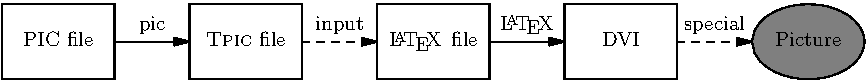
\includegraphics[width=\linewidth]{images/tpicsample}
 \caption{\Tpic �����}\figlab{tpicsample}
\end{center}
\end{figure}
{\PIC}�����ϥե�����\fl{tpicsmpl.pic}�˰ʲ���
�褦�ʵ��Ҥ򤷤ޤ���

\begin{InText}
.PS
 box "PIC file" 
 arrow "pic" above 
 box "\textsc{Tpic} file"
 arrow "input" above dashed
 box "{\LaTeX} file"
 arrow "{\LaTeX}" above
 box "DVI"
 arrow "special" above dashed
 ellipse "Picture" fill
.PE
\end{InText}

����\fl{tpicsmpl.pic}��\prog{pic}��{\TeX}�Ѥ˽���
���뤿��� \copt{-t} ���ץ������դ���
\begin{InTerm}
   \type{pic -t tpicsmpl.pic > tpicsmpl.tex}
\end{InTerm}
�Ȥ������\fl{tpicsmpl.tex}��� \cmd{graph}�˿޷�
����Ǽ����ޤ��������\fl{file.tex}�ǻ��Ѥ��뤿��ˤ�
���Τ褦�� \cmd{input}̿��ǥե�������ɤ߹��ߡ�\cmd{box}̿���
�ºݤ˿ޤ���Ѥ��ޤ���

\begin{InTeX}
\input{tpicsmpl} 
\begin{center}
  {\box\graph}
\end{center}
\end{InTeX}

����Ȥ��ξ������·���ǥ���դ������Ǥ��ޤ���
Ŭ��\env{figure}�Ķ��������ʤɤ��ޤ���
\end{Exe}

\begin{Prob}
����~\ref{exe:tpicsample}�Ǻ��������ե����� \fl{tpicsmpl.tex}
�����ľ�ܱ������ƤߤƤ�������������ȤɤΤ褦�ʵ��Ҥ�����Τ���
��ǧ�Ǥ���Ȼפ��ޤ���

����Ū�ˤϿ�¿���� \C{special} ̿���Ȥäơ�\str{pn}, \str{pa},
\str{fp}, \str{sh}��ǥХ����ɥ饤�Ф��Ϥ��Ƥ���Ȥ������ˤʤäƤ��ޤ���
�����ǡ��㤨��`\verb|\special{pa 4500 0}|'�Τ褦�ʵ��Ҥ򤤤��Ĥ�������
�����Ȥ��Ƥߤơ�����̿�᤬�ɤΤ褦��������äƤ���Τ����ͤ��ƤߤƤ���
������
\end{Prob}

\begin{Prob}
\unixos �Ǥ���Х��󥽡��뤫�� \type{man pic}�Ȥ��ơ��ɤΤ褦��
ɽ��ǽ�Ϥ�����Τ����ǧ���ƤߤƲ�����������ˤ�ꡤ
\str{for}, \str{if}, \str{sin}, \str{cos} ���Υ��ޥ�ɤ�
���ѤǤ������ʬ����Ȼפ��ޤ���
\end{Prob}


\subsection{�᥿������ץ������}
\zindind{�ե����}{�Υǥ�����}%
\Person{Donald}{Knuth}���ե���ȥǥ������Ѥ˳�ȯ
����\Prog[MetaFont]{\MF}������ޤ���������Ф�
��\Person{John}{Hobby}������˴ؤ��륢�르�ꥺ���%
�ɲä����ꡤ���Ϸ�����EPS�ˤ���\Prog[MetaPost]{\MP}
�Ȥ�������ץ�������ȯ���ޤ�����{\MF}��{\TeX}
�Υե���ȷ����ե�����\Va{file}{gf}����Ϥ���Τ�
�Ф���{\MP}��EPS�����ե�����\Va{file}{n}�����
����ΤǺ��Ǥ�{\MP}�������Ȥ�줤�ޤ���
{\MP}�˴ؤ������ܸ����Ͼ��ʤ��Τ������Ǥ���
������{\MF}�����ѹ����ɲä��줿�ս꤬���ä�
�Ȥ��Ƥ⡤\Person{Donald}{Knuth}��
\emph{\MF book}~\cite{metafontbook}�����ͤˤ�
��Ȼפ��ޤ���

{\MF}�����äȿ��äƤߤޤ��礦�����󥽡��뤫��
\begin{InTerm}
   \type{mf} 
\end{InTerm}
�Ȥ���ȥ������ꥹ��\qu{\str{*}}�����ɽ�����졤
�ե���������Ϥ�¥���Ƥ��ޤ���

\begin{OutTerm}
This is METAFONT, Version 2.7182 (Web2C 7.3.9)
**
\end{OutTerm}

�����Ǥϼ¸�Ū�ˡ�
\qq{\cmd{relax}}�����Ϥ��Ʋ��Ԥ��ޤ��������
�������ꥹ������Ĥˤʤ�Ϥ��Ǥ���
\begin{InTerm}
   \type[**]{\relax}
\end{InTerm}
����ǽ����������Ǥ����Ȥꤢ��������ɽ�����Ƥߤޤ��礦��
\begin{InTerm}
   \type[*]{drawdot (0,0); showit;}
\end{InTerm}
���٤�ľ�������������
\begin{InTerm}
   \type[*]{draw (0,0)..(100,0); showit;}
\end{InTerm}
�Ȥ��Ƥߤޤ��礦�������ʤɤ�
\begin{InTerm}
   \type[*]{draw (0,100)..(100,100)..(100,0); showit;}
\end{InTerm} 
�Ȥ����ʷ�ϵ����Ĥ����Ǥ��礦��
��λ����Ȥ���
\begin{InTerm}
   \type[*]{end.}
\end{InTerm}
�����Ϥ��ޤ���

���٤�{\MP}�򾯤��θ����Ƥߤޤ��礦��\qu{\prog{mp}}
��\qu{\prog{mpost}}�򥳥󥽡��뤫��¹Ԥ�����ɤ��Ϥ��Ǥ���
���٤�{\MP}�Υե�����\fl{hoge.mp}���Ѱդ��ޤ���

\begin{InText}
beginfig(1)
u=100;
draw (u,u)--(2u,u)--(2u,2u)..cycle;
draw (u,u)..(2u,u)..(2u,2u)..(u,2u)..cycle;
endfig;
end. 
\end{InText}

����򸫤Ƥⲿ���ʤ�����狼��ޤ��󤬡�
�Ȥꤢ������¸���Ƥ����ޤ������󥽡��뤫��
\begin{InTerm}
\type{mpost hoge.mp}
\end{InTerm}
�Ȥ��ޤ������������EPS������\fl{hoge.1}������
����ޤ��ΤǤ�������������\prog{\GS}�ʤɤ�
�����\figref{mpsample}�Τ褦�ʱߤȤ��αߤ�
���ܤ���ľ�������ջ��ѷ���ɽ������ޤ���
\begin{figure}[htbp]
 \begin{center}
  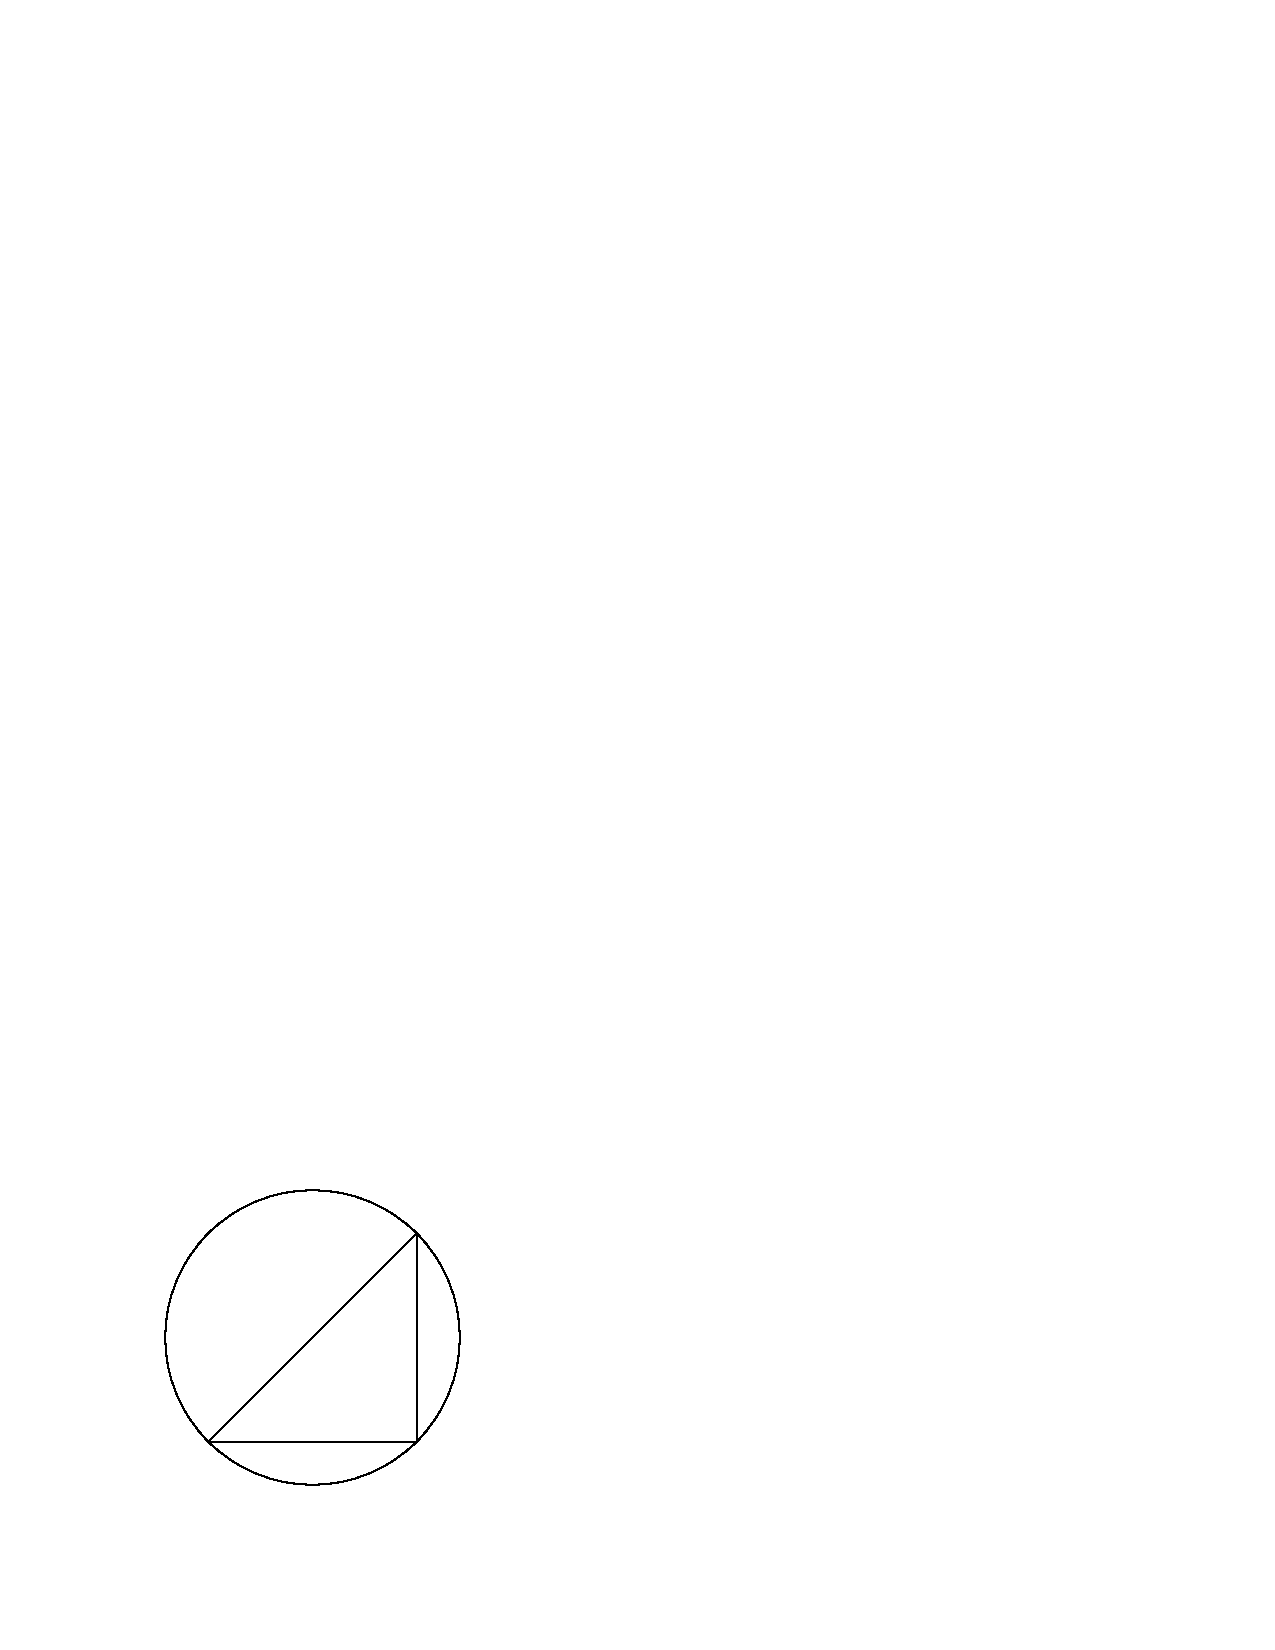
\includegraphics[clip,bb={74 74 225 225}]{images/mpsample}
  \caption{{\protect\MP}�����}\figlab{mpsample}
 \end{center}
\end{figure}
�Ķ��ˤ�äƤ����ܸ첽���줿{\MP}��Ȥ�����ˤ�
\prog{mpost}�ǤϤʤ�\prog{jmpost}��Ȥ�����
�ʤ뤫�⤷��ޤ���\Hito{��ƣ}{μ}��{\pTeX}��
�ȤäƤ���Windows������\prog{jmpost}�ΤϤ��Ǥ���


\subsection{\textsf{PSTricks}}
\Person{Timothy}{Zandt}��ˤ��\Sty{PSTricks}�� \cmd{special}̿
�����{\PS}̿��򵭽Ҥ�����ˤ�ä�{\PS}�����赡ǽ��
{\laTEX}�ǻȤ���褦�ˤ���ѥå������Ǥ���{\PS}̿
���¿�Ѥ��������ǥХ����ɥ饤�ФȤ���\Prog{dvips}
�ʤɤ����ꤷ�Ƥ�����{\PS}�б��ץ�󥿤Ǥλ��Ѥ��侩����
�ޤ���\sty{PSTricks}�ξܤ����Ȥ��������ܸ�����70�ڡ���ʬ��
\wasyo{\GCOMP}\cite{graphicscomp}����4�Ϥ򻲾Ȥ��Ƥ���������
����Ū�ʥޥ������ɤ߹��ि��ˤ�\sty{PSTricks}�ѥå��������ɤ�
���ߤޤ�������Υѥå���������̤��ɤ߹������Ǥ��ޤ���
����Ȥ�����ˤ�\sty{grahics}�ѥå������˴ޤޤ��\Sty{color}
�ѥå������ǤϤʤ�\Sty{pst-col}�ѥå��������ɤ߹��ߤޤ�������
�ε�ǽ��Ȥ��Ȥ���\Sty{pst-all}���ɤ߹��ޤ���ɸ��Ū�˰ʲ��Τ�
���ˤ���Ȥ��ޤ��Ԥ��Ȼפ��ޤ���

\begin{InTeX}
\usepackage[dvips]{graphicx}
\usepackage[dvips,usenames]{pst-col} 
\usepackage{pst-all}
\end{InTeX}

����Ū��\Z{�������ͱ�}��������EPS�Ѵ���\Z{����ǡ������}��
\Z{�ڹ�¤}��\Z{��ϩ��}��\Z{�ץ��å�}�ʤɤ��ޤ��ޤʻ����Ǥ��ޤ���
%\kutiref{pstricks}�˾������ܿޤ���򼨤��ޤ���

\sty{PSTricks}��\Prog[dvipdfmx]{\Dvipdfmx}��
�Ȥ��ˤϤޤ����ݤ���ˡ�Ȥ���\sty{PSTricks}��
�Ȥä��������޷����İ��EPS�ե�������Ѵ�������ˡ������ޤ���

\begin{InTeX}
\documentclass{jsarticle}
\usepackage[dvips]{graphicx}
\usepackage[dvips,usenames]{pst-col} 
\usepackage{pst-all}
\pagestyle{empty}
\begin{document}
\begin{pspicture}(100,100)
 ��������
\end{pspicture}
\end{document}
\end{InTeX}

���Τ褦�ʥե�����\fl{fig1.tex}�������������򥳥󥽡��뤫��
���Τ褦�ˤ��ޤ���
\begin{InTerm}
\type{platex fig1}
\type{dvipsk -Pdl -E -o fig1.eps fig1}
\type{epstopdf fig1.eps}
\type{egrep} \verb|"^%%BoundingBox:" fig1.eps > fig1.bb|
\end{InTerm}

�嵭������޷��ο��������ʤ����޷�����Ѥ�����
{\LaTeX}�θ��Ƥ�PDF�ե�����\fl{fig1.pdf}�Ȥ���
\sty{graphicx}�� \cmd{includegraphics}��ĥ����ߤޤ���

\begin{InTeX}
\usepackage[dvipdfmx]{graphicx}
\includegrpahics[bb={0 0 100 100}]{fig1.pdf}
\end{InTeX}

\Person{CV}{Radhakrishnan}��\Person{CV}{Rajagopal}���
���\Sty{pdftricks}��Ȥ��Ⱦ����ϳڤˤʤ�ޤ���
����Ϥ�Ȥ��\prog{pdf\TeX}��\sty{PSTricks}��
�Ȥ�����Τ�ΤǤ�����\prog{\pLaTeX}�ˤ�ή�ѤǤ�
�����Ǥ����ޤ���\sty{pdftricks}����°��
\Prog{pst2pdf}�Ȥ��������륹����ץȤ򾯤��ѹ�
���ޤ���

\begin{InText}
for f in $FIGURES ; do
  latex $fig
  dvips -Ppdf -E -o $fig.eps $fig
  epstopdf $fig.eps 
done
\end{InText}

������ʬ��\qu{\str{latex}}�Ϥ������\qu{\str{platex}}
�ˤ��ޤ�����\qu{\str{dvips}}�⤴��ʬ�Υ����ƥ��
�礦�褦���ѹ����Ƥ���������\Prog{epstopdf}��
�Ѵ�����PDF�ΥХ���ǥ��󥰥ܥå���������Ǥ�����
������������꤬���ä����ϼ���1�Ԥ��ɲä��Ƥ������ɤ��Ǥ��礦��

\begin{InText}
    egrep "^%%BoundingBox:"      $FILE > $fig.bb 
\end{InText}

%���Ȥ�
%\begin{InTerm}
%   \type{platex file}
%   \type{pst2pdf file}
%   \type{platex file}
%   \type{dvipdfmx file}
%\end{InTerm}
%�Τ褦�ʺ�Ȥ򤷤ޤ���
%\sty{graphicx}��\sty{color}
%�ѥå��������ɤ߹���Ȥ���
%\begin{InText}
%\usepackage[dvipdfm]{graphicx,color} 
%\end{InText}
%�Τ褦��\Option{dvipdfm}���դ��ޤ���

\subsection{Xy-pic}
\Z{�����������}�ʤɤ������ˤ�\Person{Kristoffer}{Rose}��
\Person{Ross}{Moore}�ˤ��\Prog[Xy-pic]{\Xy-pic}�ѥå�
������Ȥ����ɤ��Ǥ��礦��\Z{�������ܿ�}��\Z{�����ȥޥȥ�}��
\Z{��ϩ��}�ʤɤ����������Ǥ������������줿�����ƥ��
�ʤäƤ��ޤ����ܺ٤�\wasyo{\GCOMP}\cite{graphicscomp}
����5�Ϥ򻲾Ȥ��Ƥ���������

\subsection{���ؼ������ع�¤��}\zindind{����}{��}\zindind{����}{��¤��}
���ؼ��䲽�ع�¤������������ˤϡ�\Hito{ƣ��}{�ú�}�ˤ��
\ruby{\XyMTeX}{�����Ƥ�}�ѥå�������Ȥ����ɤ�
�Ǥ��礦�������{\LaTeX}��\env{picture}�Ķ���
\sty{epic}��Ȥäƥ٥󥼥�Ĥ䤽��¾¿���β��ؼ���
���������Ǥ��ޤ���\Prog[XyMTeX]{\XyMTeX}�ˤĤ���
�ܤ����Τꤿ������\hito{ƣ��}{�ú�}�ν񤤤�
\yousyo{\XyMTeX}~\cite{xymtex}�򻲾Ȥ��Ƥ���������


%\subsection{�������侭��}
%��ݡ��Ȥ���ʸ�dz����������������ʤɤοޤ�
%�����ͤϾ������Ȼפ��ޤ������ܤ������Ȥ�
%\wasyo{\GCOMP}\cite{graphicscomp}����7�Ϥ�
%��8�Ϥ򻲾Ȥ��Ƥ���������
%
% hoge hoge


\subsection{����դ�����}\seclab{gnuplot}
{\LaTeX}�˥���դ���������ˤ��͡�����ˡ��
����ޤ���Windows�����Ǥʤ��{Excel}�Ǻ�������
����դ�EPS����¸���������\textsf{graphicx}��
�å��������ɤ߹���Ȥ�����ˡ\pp{\secref{picture:program}����}������ޤ���
����ɽ�׻����եȤʤ�ƻȤ������ʤ�����
\Person{Thomas}{Williams}��\Person{Colin}{Kelley}��ˤ��
\Prog{Gnuplot}��Ȥ����ɤ��Ǥ��礦��\prog{gnuplot}
�ϥС������3.7�˴ؤ��Ƥ�\Hito{����}{����}�����С�����
��3.8�˴ؤ��Ƥ�\Hito{����}{��}���ץ����������ܸ첽��
����Ƥ��ޤ����ޤ�\prog{gnuplot}�Υޥ˥奢���
�ؤ��Ƥ�\Hito{����}{�м�}��ˤ�äƹԤ��Ƥ��ޤ�\footnote{\webGplotman}��

\Z{�����}�Ǥ�\Prog{SciLab}�Ȥ����Τ�����ޤ���
�ޥ˥奢�뤬\Hito{����}{����}��ˤ�ä����ܸ첽����Ƥ��ޤ�\footnote{\webScilabman}��

\Person{John}{Eaton}��ˤ��\Prog{Octave}�Ȥ����Τ⤢��ޤ�
�Τ�Ĵ�٤ƤߤƤ���������

\endinput

%�ܽ�Ǥϥ��������Τ���Υץ��åȥ��եȤβ���򤷤ޤ���
%���Ǥ������λ��ͽ�����ܸ첽�ޥ˥奢�뤬����ޤ��Τǡ�
%\appref{info}�򻲾Ȥ��Ƥ���������

%
%
%\subsection{����Ū�����}
%�ޤ�{Gnuplot}�����÷��Υ��եȥ������Ǥ������÷��Ȥ������޷��ʤɤ�
%���ץ����ʤɤ���ꤷ�ʤ���������ǧ���Ƥ������֤Τ��ȤǤ���
%{Windows}�Ǥ�{Gnuplot}�򥤥󥹥ȡ��뤷��`\texttt{Readme}'���ɤ���塤
%\texttt{wgnuplot}��¹Ԥ���С�
%\begin{quote}
%\verb+gnuplot> +
%\end{quote}
%�Ȥ������֤ˤ���Ȼפ��ޤ����桼����������Ϥ��Ե����Ƥ�����֤Ǥ���
%ư����{Unix}�ϤΥ�����˻��Ƥ��ޤ���
%����󥰥ǥ��쥯�ȥ�γ�ǰ�⤢��ޤ���
%��λ��\texttt{exit}�Ǥ��Ĥ���ܥ���Ǥ⤫�ޤ��ޤ���
%������
%\begin{quote}
%\verb+gnuplot> help+
%\end{quote}
%�Ȥ����{Windows}�ʤ�бѸ�Υإ�פ�ɽ�������Ǥ��礦��
%����Ĥ��Ǥ狼��䤹����ΤǤ��Τǡ������̤����ɤ�Ǥߤ�
%���Ȥ򤪴��ᤷ�ޤ���
%
%��������դ�ɽ�����Ƥߤޤ��礦��
%\begin{quote}
%\verb+gnuplot>plot sin(x)+
%\end{quote}
%�Ȥ�����̥�����ɥ���������sin�ؿ���ɽ�����줿�Ȼפ��ޤ���
%\subsection{�Ф��륳�ޥ��}
%�ޤ��Ϥ�������ϲ������Ƥ������ۤ����ɤ����ޥ�ɤ�\tabref{gnuplotcmd}
%�˵����ޤ����롼��Ȥ��ƥե�����̾��ǥ��쥯�ȥ�̾����٥�̾�ʤɡ�
%ʸ����ϥ��󥰥륯�����Ȥ����֥륯�����ȤǰϤळ�Ȥ�ɬ�פǤ���
%\begin{table}[htbp]
%\caption{{Gnuplot}�δ��ܥ��ޥ��}\tablab{gnuplotcmd}
%\begin{center}
%\begin{tabular}{|l|l|l|}
%\hline
%̿�� & ���� & ���� \\
%\hline
%\texttt{exit}   & {Gnuplot}��λ���ޤ� & �ʤ� \\
%\texttt{cd}     & ��ȥե�������ѹ����ޤ� &  '�ǥ��쥯�ȥ�̾'\\
%\texttt{pwd}    & ���ߤκ�ȥե������ɽ�����ޤ� & �ʤ� \\
%\texttt{help}   & �إ�פ�ɽ�����ޤ� &  �������\\
%\texttt{load}   & �ե�������ɤ߹��ߤޤ� &  '�ե�����̾'\\
%\texttt{plot}   & 2�����Ǵؿ���ǡ�����ץ��åȤ��ޤ� & �ؿ��ʤ� \\
%\texttt{splot}  & 3�����Ǵؿ���ǡ�����ץ��åȤ��ޤ� & �ؿ��ʤ� \\
%\texttt{multiplot}&ʣ���δؿ���ǡ������Ĥ����ɽ�����ޤ�& �ؿ��ʤ�\\
%\texttt{replot} & ����ɽ��������Τ�⤦���٥ץ��åȤ�ľ���ޤ� & �ʤ� \\
%\texttt{set}    & ���ץ��������ꤷ�ޤ� & ¿�� \\
%\hline
%\end{tabular}
%\end{center}
%\end{table}
%�Ȥ⤫����\texttt{plot}�Ȥ������ޥ�ɤDz��Ǥ������Ȥ������ȤǤ���
%\texttt{plot}���ޥ�ɤǤ�ʣ���δؿ���ʣ���Υǡ���
%(\secref{gnuplotdatafile}����)��ץ��åȤ��뤳�Ȥ���ǽ�Ǥ���
%�ޤ����ѿ�������������`A=35'�ʤɤΤ褦��ñ��ˤǤ��ޤ���
%
%\subsection{�ؿ��ȱ黻��}\seclab{gnuplot:functions}
%��������Ѥߤδؿ��ˤĤ��ƤǤ���
%Gnuplot�Ǥ��͡��ʴؿ����Ѱդ���Ƥ��ޤ���
%�ۤȤ�ɤ�����Ѥߴؿ���`�ؿ�(�ѿ�$x$)'��
%`sin($x$)'�Τ褦�˻Ȥ��ޤ���
%\tabref{gnuplot:functions}�˼��פ�����Ѥߴؿ���ܤ��Ƥ����ޤ���
%\begin{table}[htbp]
%\caption{Gnuplot�μ������Ѥߴؿ�}
%\tablab{gnuplot:functions}
%\begin{center}
%\begin{tabular}{|ll|ll|}
%\hline
%�ؿ�     & ����         &  �ؿ�    &  ���� \\
%\hline
%\verb+sin(x)+   & ����         & \verb+log(x)+   & �����п�\\
%\verb+asin(x)+  & ������       & \verb+log10(x)+ & �����п�\\
%\verb+asinh(x)+ & ���ж������� & \verb+exp(x)+   & �ؿ��ؿ�\\
%\verb+cos(x)+   & ;��         & \verb+int(x)+   & $x$������\\
%\verb+acos(x)+  & ��;��       & \verb+sqrt(x)+  & $x$��ʿ����\\
%\verb+asinh(x)+ & �����;�� & \verb+abs(x)+   & $x$��������\\
%\verb+tan(x)+   & ����         & \verb+rand(x)+  & 0����1̤�������$\times x$\\
%\verb+atan(x)+  & ������       & \verb+imag(z)+  & z���\\
%\verb+atanh(x)+ & ���ж������� & \verb+real(z)+  & z�μ���\\
%\hline
%\end{tabular}
%\end{center}
%\end{table}
%�ʾ�Υ��ޥ�ɤȴؿ������򤷤��顤
%���٤Ϥ���˴ؤ��\Z{�黻��}���ͤ�
%���ޤ����黻�Ҥ�ɽ����ˡ��C����Ȼ��Ƥ��ޤ���
%`���Ƥ���'�Ȥ����Τ�ɽ���Τ��������ǤϤʤ��������Τ����Ǥ⤽���Ǥ���
%����Ʊ�Τν������������㤨��`$7/2=3$'�Ȥʤꡤɬ�������ˤʤ�ޤ���
%�ޤ����黻�Ҥˤ�äƤ�����Ʊ�ΤΤߤΤ�Τ⤢��ޤ���
%ɽ���ˤ����ơ��٤������ɽ����ˡ����äơ�
%FORTRAN�Τ褦�˥������ꥹ��`*'�����³����`**'��ɽ�����ޤ���
%�黻�Ҥ�ñ��黻��(Unary)�����黻��(Binary)��
%����黻��(Ternary)����ʤ�ޤ���
%Gnuplot�μ�ʱ黻�Ҥ�\tabref{gnuplot:Operators}���̤�Ǥ���
%�ʤ����Ʊ黻�Ҥ�ͥ���̤�C����Ȥۤ�Ʊ���Ǥ��Τ�Ŭ��
%���`()'�dz��ʤɤ��б����Ƥ���������
%\begin{table}[htbp]
%\caption{Gnuplot�μ�ʱ黻��}
%\tablab{gnuplot:Operators}
%\begin{center}
%*���դ��Ƥ���黻�Ҥΰ����������˸¤�ޤ�\\
%\begin{tabular}{|l|l|l@{$= $ }l|}
%\hline
%�黻��    & ����             & ��   & ������ \\\hline
%\multicolumn{4}{|c|}{1��黻��}\\\hline
%\verb+-+ & ��                & -5   & -5     \\
%\verb-+- & ��                & +5   & +5     \\
%\verb+!+ & *����             & 4!   & 24     \\
%\verb+$+ & *`using'���������& \$ 3 &        \\\hline
%\multicolumn{4}{|c|}{2��黻��}\\\hline
%\verb+**+& �٤���            & 2**10& 1024   \\
%\verb+*+ & �軻              & 2*5  & 10     \\
%\verb+/+ & ����              & 7/2  & 3      \\
%\verb+%+ & *��;             & 7\%2 & 1      \\
%\verb-+- & �û�              & 7+2  & 9      \\
%\verb+-+ & ����              & 7-2  & 5      \\\hline
%\end{tabular}
%\end{center}
%\end{table}
%
%\subsection{���ץ���������}
%����������������Ǥ���­�Τ�������դ������ޤ����̾�$x$���Υ�٥��
%�ϰϻ���ʤɤ�ɬ�פˤʤ�ޤ������Τ褦�ʤȤ���`\texttt{set}'
%���ޥ�ɤ�Ȥ��ޤ���Gnuplot��\texttt{set}���ޥ�ɤǥ���
%�դ˴ؤ��������Ԥ��ޤ�����ʥ��ץ�����
%\tabref{gnuplot:options}�˼����ޤ���
%
%\begin{table}[htbp]
%\caption{Gnuplot�μ��ץ��ץ����}\tablab{gnuplot:options}
%\begin{center}
%`()'���ͤ�Ǥ�դǤ���`\{\}'���ͤϤ����줫��Ĥ����Ӥޤ���\\
%\begin{tabular}{|l|l|l|}
%\hline
%����               & ���� & ���� \\\hline
%\verb+data style+         & �ǡ�����ɽ�������λ��� & \texttt{lines��points,...}\\
%\verb+function style+     & �ؿ���ɽ�������λ���   & \texttt{lines��points,...}\\
%\verb+(no)grid+           & �ʻ�����(��)ɽ��       & \texttt{(no)x(2)tics}\\
%\verb+(no)key+            & ̾����(��)ɽ��         & \texttt{left,right,...}\\
%\verb+(no)logscale+       & �п�������(���ʤ�)���� & \texttt{x,y,z,xy,...}\\
%\verb+output+             & ��������           & \texttt{'filename.tex'} \\
%\verb+{xyz}(2)range+      & �Ƽ����ϰϻ���         & \verb+[�Ǿ���:������]+ \\
%\verb+samples+            & �ץ��åȤ�������       & 1����礭����\\
%\verb+size ��,�⤵+       & ���Ϥ��륰��դ��礭�� & $0<$��$\leq 1$\\
%\verb+terminal+           & ���ϥǥХ���������     & \texttt{eepic,tgif,...}\\
%\verb+(no){xyz}(2)tics+   & ��������դ����λ���   & �����,�ֳ�,����\\
%\verb+(no){xyz}(2)label+  & �ƥ�٥�λ���         & 'ɽ������̾��'\\\hline
%\end{tabular}
%\end{center}
%\end{table}
%�Ȥ�����
%\begin{quote}
%\verb+gnuplot> set ���� ����1 ����2...+\\
%\verb+gnuplot> set xtics 0,1,10+
%\end{quote}
%��������Ǥ���
%
%\begin{comment}
%�⤦�����狼��䤹���ºݤΥ���դ��б��������\figref{gnuplot:taiou}
%�Ȥʤ�ޤ���
%\begin{figure}[htbp]
%  \begin{center}
%  \begin{minipage}{.9\textwidth}
%    \begin{minipage}{.47\textwidth}
%      \begin{center}
%        \input{gnuplottaiou1}
%        (a)���ץ����ι���
%      \end{center}
%    \end{minipage}
%  \hfill
%    \begin{minipage}{.47\textwidth}
%      \begin{center}
%        \input{gnuplottaiou2}
%        (b)���ܸ�Ǥβ���
%      \end{center}
%    \end{minipage}
%  \end{minipage}
%  \caption{Gnuplot���ץ����ο޲�}\figlab{gnuplot:taiou}
%  \end{center}
%\end{figure}
%\figref{gnuplot:taiou}(a)�Τۤ������ץ����ι��ܤ��б�����
%\figref{gnuplot:taiou}(b)�����ܸ�Ǥ������Ǥ���
%\end{comment}
%
%\subsection{���դ��٤�����}
%�黻�Ҥ�ͥ���̤䡤�黻���٤ˤĤ��ƤϤ����褽C�����Ʊ���ʤΤǡ�
%C������ΤäƤ���Ф����˻Ȥ����ʤ���Ȼפ��ޤ���
%�������������ͤȼ��ˤĤ��Ƥ����դ�ɬ�פǤ���
%�ޤ������ͤˤĤ��ƤǤ�����Gnuplot���ͤ�������Ϳ������ȡ��黻�⤽��
%������ͥ�褷�ޤ����Ȥꤢ������Ϳ����ǡ����Ͼ����Τۤ�����̤����٤�
%�ɤ��褦�Ǥ����ޤ������ˤĤ��ƤǤ�����Gnuplot�Ǥϼ��λ��꤬��Ĥ���ޤ���
%
%\subsection{�ǡ����ե����뤫����ɤ߹���}\seclab{gnuplotdatafile}
%�������\Prog{Cygwin}�򳫤��ޤ��礦��\Prog{perl}��
%��ñ�ʥ�����ץȤ�񤭤ޤ���
% ���Υ�����ץȤϷ��Ū��Gnuplot
%��$-10 \leqq  x \leqq 10$���ϰϤ�$ y = x^3 $�Υ���դ�ץ��åȤ��Ƥ���ޤ���
%�ޤ����ʲ��Τ褦��`\texttt{Xcubed.pl}'��������ޤ���
%\begin{quote}
%\verb?for($i=-10.0; $i<=10; $i+=0.1){print "$i ",$i*$i*$i,"\n";}?
%\end{quote}
%�Ȥ����ե�������ä��Ȥ��ޤ���
%����ǡ�
%\begin{InTerm}
%   \type{perl Xcubed.pl > plot.dat}
%\end{InTerm}
%�Ȥ��ơ����ν��Ϸ�̤�`\texttt{plot.dat}'�Ȥ����ե������
%�񤭽Ф��ޤ���`\texttt{plot.dat}'�����Ƥϰʲ���\figref{plot.dat}�Τ褦�ˤʤ�ޤ���
%\begin{figure}[htbp]
%\begin{center}
%\begin{InText}
%-10               -1000
%-9.9              -970.299
%...etc...
%9.89999999999996  970.298999999989
%9.99999999999996  999.999999999989
%\end{InText}
%\end{center}
%\caption{Perl�ǽ��Ϥ��줿`plot.dat'������}\figlab{plot.dat}
%\end{figure}
%���Υǡ�����n��2��Υǡ����ˤʤäƤ��ޤ���
%���������顤���٤�Gnuplot��ư����
%\begin{InTerm}
%gnuplot >  plot 'plot.dat'
%\end{InTerm}
%�Ȥ���С�$y=x^3$�Υ���դ������ޤ���
%���η�̤�\figref{gnuplot1}(a)`���ץ�������ʤ�'�ˤʤ�ޤ���
%\begin{figure}[htbp]
%    \begin{minipage}{.47\textwidth}
%      \begin{center}
%        % GNUPLOT: LaTeX picture using EEPIC macros
\setlength{\unitlength}{0.23pt}
\begin{picture}(750,450)(0,0)
\footnotesize
\thicklines \path(176,90)(196,90)
\thicklines \path(683,90)(663,90)
\put(154,90){\makebox(0,0)[r]{-1000}}
\thicklines \path(176,122)(196,122)
\thicklines \path(683,122)(663,122)
\put(154,122){\makebox(0,0)[r]{-800}}
\thicklines \path(176,153)(196,153)
\thicklines \path(683,153)(663,153)
\put(154,153){\makebox(0,0)[r]{-600}}
\thicklines \path(176,185)(196,185)
\thicklines \path(683,185)(663,185)
\put(154,185){\makebox(0,0)[r]{-400}}
\thicklines \path(176,216)(196,216)
\thicklines \path(683,216)(663,216)
\put(154,216){\makebox(0,0)[r]{-200}}
\thicklines \path(176,248)(196,248)
\thicklines \path(683,248)(663,248)
\put(154,248){\makebox(0,0)[r]{0}}
\thicklines \path(176,280)(196,280)
\thicklines \path(683,280)(663,280)
\put(154,280){\makebox(0,0)[r]{200}}
\thicklines \path(176,311)(196,311)
\thicklines \path(683,311)(663,311)
\put(154,311){\makebox(0,0)[r]{400}}
\thicklines \path(176,343)(196,343)
\thicklines \path(683,343)(663,343)
\put(154,343){\makebox(0,0)[r]{600}}
\thicklines \path(176,374)(196,374)
\thicklines \path(683,374)(663,374)
\put(154,374){\makebox(0,0)[r]{800}}
\thicklines \path(176,406)(196,406)
\thicklines \path(683,406)(663,406)
\put(154,406){\makebox(0,0)[r]{1000}}
\thicklines \path(176,90)(176,110)
\thicklines \path(176,406)(176,386)
\put(176,45){\makebox(0,0){-10}}
\thicklines \path(227,90)(227,110)
\thicklines \path(227,406)(227,386)
\put(227,45){\makebox(0,0){-8}}
\thicklines \path(277,90)(277,110)
\thicklines \path(277,406)(277,386)
\put(277,45){\makebox(0,0){-6}}
\thicklines \path(328,90)(328,110)
\thicklines \path(328,406)(328,386)
\put(328,45){\makebox(0,0){-4}}
\thicklines \path(379,90)(379,110)
\thicklines \path(379,406)(379,386)
\put(379,45){\makebox(0,0){-2}}
\thicklines \path(430,90)(430,110)
\thicklines \path(430,406)(430,386)
\put(430,45){\makebox(0,0){0}}
\thicklines \path(480,90)(480,110)
\thicklines \path(480,406)(480,386)
\put(480,45){\makebox(0,0){2}}
\thicklines \path(531,90)(531,110)
\thicklines \path(531,406)(531,386)
\put(531,45){\makebox(0,0){4}}
\thicklines \path(582,90)(582,110)
\thicklines \path(582,406)(582,386)
\put(582,45){\makebox(0,0){6}}
\thicklines \path(632,90)(632,110)
\thicklines \path(632,406)(632,386)
\put(632,45){\makebox(0,0){8}}
\thicklines \path(683,90)(683,110)
\thicklines \path(683,406)(683,386)
\put(683,45){\makebox(0,0){10}}
\thicklines \path(176,90)(683,90)(683,406)(176,406)(176,90)
\put(509,364){\makebox(0,0)[r]{"plot.dat"}}
\put(176,90){\raisebox{-1.2pt}{\makebox(0,0){$\Diamond$}}}
\put(179,95){\raisebox{-1.2pt}{\makebox(0,0){$\Diamond$}}}
\put(181,99){\raisebox{-1.2pt}{\makebox(0,0){$\Diamond$}}}
\put(184,104){\raisebox{-1.2pt}{\makebox(0,0){$\Diamond$}}}
\put(186,108){\raisebox{-1.2pt}{\makebox(0,0){$\Diamond$}}}
\put(189,113){\raisebox{-1.2pt}{\makebox(0,0){$\Diamond$}}}
\put(191,117){\raisebox{-1.2pt}{\makebox(0,0){$\Diamond$}}}
\put(194,121){\raisebox{-1.2pt}{\makebox(0,0){$\Diamond$}}}
\put(196,125){\raisebox{-1.2pt}{\makebox(0,0){$\Diamond$}}}
\put(199,129){\raisebox{-1.2pt}{\makebox(0,0){$\Diamond$}}}
\put(201,133){\raisebox{-1.2pt}{\makebox(0,0){$\Diamond$}}}
\put(204,137){\raisebox{-1.2pt}{\makebox(0,0){$\Diamond$}}}
\put(206,140){\raisebox{-1.2pt}{\makebox(0,0){$\Diamond$}}}
\put(209,144){\raisebox{-1.2pt}{\makebox(0,0){$\Diamond$}}}
\put(211,148){\raisebox{-1.2pt}{\makebox(0,0){$\Diamond$}}}
\put(214,151){\raisebox{-1.2pt}{\makebox(0,0){$\Diamond$}}}
\put(217,154){\raisebox{-1.2pt}{\makebox(0,0){$\Diamond$}}}
\put(219,158){\raisebox{-1.2pt}{\makebox(0,0){$\Diamond$}}}
\put(222,161){\raisebox{-1.2pt}{\makebox(0,0){$\Diamond$}}}
\put(224,164){\raisebox{-1.2pt}{\makebox(0,0){$\Diamond$}}}
\put(227,167){\raisebox{-1.2pt}{\makebox(0,0){$\Diamond$}}}
\put(229,170){\raisebox{-1.2pt}{\makebox(0,0){$\Diamond$}}}
\put(232,173){\raisebox{-1.2pt}{\makebox(0,0){$\Diamond$}}}
\put(234,176){\raisebox{-1.2pt}{\makebox(0,0){$\Diamond$}}}
\put(237,179){\raisebox{-1.2pt}{\makebox(0,0){$\Diamond$}}}
\put(239,181){\raisebox{-1.2pt}{\makebox(0,0){$\Diamond$}}}
\put(242,184){\raisebox{-1.2pt}{\makebox(0,0){$\Diamond$}}}
\put(244,187){\raisebox{-1.2pt}{\makebox(0,0){$\Diamond$}}}
\put(247,189){\raisebox{-1.2pt}{\makebox(0,0){$\Diamond$}}}
\put(250,191){\raisebox{-1.2pt}{\makebox(0,0){$\Diamond$}}}
\put(252,194){\raisebox{-1.2pt}{\makebox(0,0){$\Diamond$}}}
\put(255,196){\raisebox{-1.2pt}{\makebox(0,0){$\Diamond$}}}
\put(257,198){\raisebox{-1.2pt}{\makebox(0,0){$\Diamond$}}}
\put(260,200){\raisebox{-1.2pt}{\makebox(0,0){$\Diamond$}}}
\put(262,203){\raisebox{-1.2pt}{\makebox(0,0){$\Diamond$}}}
\put(265,205){\raisebox{-1.2pt}{\makebox(0,0){$\Diamond$}}}
\put(267,207){\raisebox{-1.2pt}{\makebox(0,0){$\Diamond$}}}
\put(270,208){\raisebox{-1.2pt}{\makebox(0,0){$\Diamond$}}}
\put(272,210){\raisebox{-1.2pt}{\makebox(0,0){$\Diamond$}}}
\put(275,212){\raisebox{-1.2pt}{\makebox(0,0){$\Diamond$}}}
\put(277,214){\raisebox{-1.2pt}{\makebox(0,0){$\Diamond$}}}
\put(280,216){\raisebox{-1.2pt}{\makebox(0,0){$\Diamond$}}}
\put(282,217){\raisebox{-1.2pt}{\makebox(0,0){$\Diamond$}}}
\put(285,219){\raisebox{-1.2pt}{\makebox(0,0){$\Diamond$}}}
\put(288,220){\raisebox{-1.2pt}{\makebox(0,0){$\Diamond$}}}
\put(290,222){\raisebox{-1.2pt}{\makebox(0,0){$\Diamond$}}}
\put(293,223){\raisebox{-1.2pt}{\makebox(0,0){$\Diamond$}}}
\put(295,224){\raisebox{-1.2pt}{\makebox(0,0){$\Diamond$}}}
\put(298,226){\raisebox{-1.2pt}{\makebox(0,0){$\Diamond$}}}
\put(300,227){\raisebox{-1.2pt}{\makebox(0,0){$\Diamond$}}}
\put(303,228){\raisebox{-1.2pt}{\makebox(0,0){$\Diamond$}}}
\put(305,229){\raisebox{-1.2pt}{\makebox(0,0){$\Diamond$}}}
\put(308,231){\raisebox{-1.2pt}{\makebox(0,0){$\Diamond$}}}
\put(310,232){\raisebox{-1.2pt}{\makebox(0,0){$\Diamond$}}}
\put(313,233){\raisebox{-1.2pt}{\makebox(0,0){$\Diamond$}}}
\put(315,234){\raisebox{-1.2pt}{\makebox(0,0){$\Diamond$}}}
\put(318,235){\raisebox{-1.2pt}{\makebox(0,0){$\Diamond$}}}
\put(320,235){\raisebox{-1.2pt}{\makebox(0,0){$\Diamond$}}}
\put(323,236){\raisebox{-1.2pt}{\makebox(0,0){$\Diamond$}}}
\put(326,237){\raisebox{-1.2pt}{\makebox(0,0){$\Diamond$}}}
\put(328,238){\raisebox{-1.2pt}{\makebox(0,0){$\Diamond$}}}
\put(331,239){\raisebox{-1.2pt}{\makebox(0,0){$\Diamond$}}}
\put(333,239){\raisebox{-1.2pt}{\makebox(0,0){$\Diamond$}}}
\put(336,240){\raisebox{-1.2pt}{\makebox(0,0){$\Diamond$}}}
\put(338,241){\raisebox{-1.2pt}{\makebox(0,0){$\Diamond$}}}
\put(341,241){\raisebox{-1.2pt}{\makebox(0,0){$\Diamond$}}}
\put(343,242){\raisebox{-1.2pt}{\makebox(0,0){$\Diamond$}}}
\put(346,242){\raisebox{-1.2pt}{\makebox(0,0){$\Diamond$}}}
\put(348,243){\raisebox{-1.2pt}{\makebox(0,0){$\Diamond$}}}
\put(351,243){\raisebox{-1.2pt}{\makebox(0,0){$\Diamond$}}}
\put(353,244){\raisebox{-1.2pt}{\makebox(0,0){$\Diamond$}}}
\put(356,244){\raisebox{-1.2pt}{\makebox(0,0){$\Diamond$}}}
\put(359,245){\raisebox{-1.2pt}{\makebox(0,0){$\Diamond$}}}
\put(361,245){\raisebox{-1.2pt}{\makebox(0,0){$\Diamond$}}}
\put(364,245){\raisebox{-1.2pt}{\makebox(0,0){$\Diamond$}}}
\put(366,246){\raisebox{-1.2pt}{\makebox(0,0){$\Diamond$}}}
\put(369,246){\raisebox{-1.2pt}{\makebox(0,0){$\Diamond$}}}
\put(371,246){\raisebox{-1.2pt}{\makebox(0,0){$\Diamond$}}}
\put(374,246){\raisebox{-1.2pt}{\makebox(0,0){$\Diamond$}}}
\put(376,247){\raisebox{-1.2pt}{\makebox(0,0){$\Diamond$}}}
\put(379,247){\raisebox{-1.2pt}{\makebox(0,0){$\Diamond$}}}
\put(381,247){\raisebox{-1.2pt}{\makebox(0,0){$\Diamond$}}}
\put(384,247){\raisebox{-1.2pt}{\makebox(0,0){$\Diamond$}}}
\put(386,247){\raisebox{-1.2pt}{\makebox(0,0){$\Diamond$}}}
\put(389,247){\raisebox{-1.2pt}{\makebox(0,0){$\Diamond$}}}
\put(391,247){\raisebox{-1.2pt}{\makebox(0,0){$\Diamond$}}}
\put(394,248){\raisebox{-1.2pt}{\makebox(0,0){$\Diamond$}}}
\put(397,248){\raisebox{-1.2pt}{\makebox(0,0){$\Diamond$}}}
\put(399,248){\raisebox{-1.2pt}{\makebox(0,0){$\Diamond$}}}
\put(402,248){\raisebox{-1.2pt}{\makebox(0,0){$\Diamond$}}}
\put(404,248){\raisebox{-1.2pt}{\makebox(0,0){$\Diamond$}}}
\put(407,248){\raisebox{-1.2pt}{\makebox(0,0){$\Diamond$}}}
\put(409,248){\raisebox{-1.2pt}{\makebox(0,0){$\Diamond$}}}
\put(412,248){\raisebox{-1.2pt}{\makebox(0,0){$\Diamond$}}}
\put(414,248){\raisebox{-1.2pt}{\makebox(0,0){$\Diamond$}}}
\put(417,248){\raisebox{-1.2pt}{\makebox(0,0){$\Diamond$}}}
\put(419,248){\raisebox{-1.2pt}{\makebox(0,0){$\Diamond$}}}
\put(422,248){\raisebox{-1.2pt}{\makebox(0,0){$\Diamond$}}}
\put(424,248){\raisebox{-1.2pt}{\makebox(0,0){$\Diamond$}}}
\put(427,248){\raisebox{-1.2pt}{\makebox(0,0){$\Diamond$}}}
\put(429,248){\raisebox{-1.2pt}{\makebox(0,0){$\Diamond$}}}
\put(432,248){\raisebox{-1.2pt}{\makebox(0,0){$\Diamond$}}}
\put(435,248){\raisebox{-1.2pt}{\makebox(0,0){$\Diamond$}}}
\put(437,248){\raisebox{-1.2pt}{\makebox(0,0){$\Diamond$}}}
\put(440,248){\raisebox{-1.2pt}{\makebox(0,0){$\Diamond$}}}
\put(442,248){\raisebox{-1.2pt}{\makebox(0,0){$\Diamond$}}}
\put(445,248){\raisebox{-1.2pt}{\makebox(0,0){$\Diamond$}}}
\put(447,248){\raisebox{-1.2pt}{\makebox(0,0){$\Diamond$}}}
\put(450,248){\raisebox{-1.2pt}{\makebox(0,0){$\Diamond$}}}
\put(452,248){\raisebox{-1.2pt}{\makebox(0,0){$\Diamond$}}}
\put(455,248){\raisebox{-1.2pt}{\makebox(0,0){$\Diamond$}}}
\put(457,248){\raisebox{-1.2pt}{\makebox(0,0){$\Diamond$}}}
\put(460,248){\raisebox{-1.2pt}{\makebox(0,0){$\Diamond$}}}
\put(462,248){\raisebox{-1.2pt}{\makebox(0,0){$\Diamond$}}}
\put(465,248){\raisebox{-1.2pt}{\makebox(0,0){$\Diamond$}}}
\put(468,249){\raisebox{-1.2pt}{\makebox(0,0){$\Diamond$}}}
\put(470,249){\raisebox{-1.2pt}{\makebox(0,0){$\Diamond$}}}
\put(473,249){\raisebox{-1.2pt}{\makebox(0,0){$\Diamond$}}}
\put(475,249){\raisebox{-1.2pt}{\makebox(0,0){$\Diamond$}}}
\put(478,249){\raisebox{-1.2pt}{\makebox(0,0){$\Diamond$}}}
\put(480,249){\raisebox{-1.2pt}{\makebox(0,0){$\Diamond$}}}
\put(483,249){\raisebox{-1.2pt}{\makebox(0,0){$\Diamond$}}}
\put(485,250){\raisebox{-1.2pt}{\makebox(0,0){$\Diamond$}}}
\put(488,250){\raisebox{-1.2pt}{\makebox(0,0){$\Diamond$}}}
\put(490,250){\raisebox{-1.2pt}{\makebox(0,0){$\Diamond$}}}
\put(493,250){\raisebox{-1.2pt}{\makebox(0,0){$\Diamond$}}}
\put(495,251){\raisebox{-1.2pt}{\makebox(0,0){$\Diamond$}}}
\put(498,251){\raisebox{-1.2pt}{\makebox(0,0){$\Diamond$}}}
\put(500,251){\raisebox{-1.2pt}{\makebox(0,0){$\Diamond$}}}
\put(503,252){\raisebox{-1.2pt}{\makebox(0,0){$\Diamond$}}}
\put(506,252){\raisebox{-1.2pt}{\makebox(0,0){$\Diamond$}}}
\put(508,253){\raisebox{-1.2pt}{\makebox(0,0){$\Diamond$}}}
\put(511,253){\raisebox{-1.2pt}{\makebox(0,0){$\Diamond$}}}
\put(513,254){\raisebox{-1.2pt}{\makebox(0,0){$\Diamond$}}}
\put(516,254){\raisebox{-1.2pt}{\makebox(0,0){$\Diamond$}}}
\put(518,255){\raisebox{-1.2pt}{\makebox(0,0){$\Diamond$}}}
\put(521,255){\raisebox{-1.2pt}{\makebox(0,0){$\Diamond$}}}
\put(523,256){\raisebox{-1.2pt}{\makebox(0,0){$\Diamond$}}}
\put(526,257){\raisebox{-1.2pt}{\makebox(0,0){$\Diamond$}}}
\put(528,257){\raisebox{-1.2pt}{\makebox(0,0){$\Diamond$}}}
\put(531,258){\raisebox{-1.2pt}{\makebox(0,0){$\Diamond$}}}
\put(533,259){\raisebox{-1.2pt}{\makebox(0,0){$\Diamond$}}}
\put(536,260){\raisebox{-1.2pt}{\makebox(0,0){$\Diamond$}}}
\put(539,261){\raisebox{-1.2pt}{\makebox(0,0){$\Diamond$}}}
\put(541,261){\raisebox{-1.2pt}{\makebox(0,0){$\Diamond$}}}
\put(544,262){\raisebox{-1.2pt}{\makebox(0,0){$\Diamond$}}}
\put(546,263){\raisebox{-1.2pt}{\makebox(0,0){$\Diamond$}}}
\put(549,264){\raisebox{-1.2pt}{\makebox(0,0){$\Diamond$}}}
\put(551,265){\raisebox{-1.2pt}{\makebox(0,0){$\Diamond$}}}
\put(554,267){\raisebox{-1.2pt}{\makebox(0,0){$\Diamond$}}}
\put(556,268){\raisebox{-1.2pt}{\makebox(0,0){$\Diamond$}}}
\put(559,269){\raisebox{-1.2pt}{\makebox(0,0){$\Diamond$}}}
\put(561,270){\raisebox{-1.2pt}{\makebox(0,0){$\Diamond$}}}
\put(564,272){\raisebox{-1.2pt}{\makebox(0,0){$\Diamond$}}}
\put(566,273){\raisebox{-1.2pt}{\makebox(0,0){$\Diamond$}}}
\put(569,274){\raisebox{-1.2pt}{\makebox(0,0){$\Diamond$}}}
\put(571,276){\raisebox{-1.2pt}{\makebox(0,0){$\Diamond$}}}
\put(574,277){\raisebox{-1.2pt}{\makebox(0,0){$\Diamond$}}}
\put(577,279){\raisebox{-1.2pt}{\makebox(0,0){$\Diamond$}}}
\put(579,280){\raisebox{-1.2pt}{\makebox(0,0){$\Diamond$}}}
\put(582,282){\raisebox{-1.2pt}{\makebox(0,0){$\Diamond$}}}
\put(584,284){\raisebox{-1.2pt}{\makebox(0,0){$\Diamond$}}}
\put(587,286){\raisebox{-1.2pt}{\makebox(0,0){$\Diamond$}}}
\put(589,288){\raisebox{-1.2pt}{\makebox(0,0){$\Diamond$}}}
\put(592,289){\raisebox{-1.2pt}{\makebox(0,0){$\Diamond$}}}
\put(594,291){\raisebox{-1.2pt}{\makebox(0,0){$\Diamond$}}}
\put(597,293){\raisebox{-1.2pt}{\makebox(0,0){$\Diamond$}}}
\put(599,296){\raisebox{-1.2pt}{\makebox(0,0){$\Diamond$}}}
\put(602,298){\raisebox{-1.2pt}{\makebox(0,0){$\Diamond$}}}
\put(604,300){\raisebox{-1.2pt}{\makebox(0,0){$\Diamond$}}}
\put(607,302){\raisebox{-1.2pt}{\makebox(0,0){$\Diamond$}}}
\put(609,305){\raisebox{-1.2pt}{\makebox(0,0){$\Diamond$}}}
\put(612,307){\raisebox{-1.2pt}{\makebox(0,0){$\Diamond$}}}
\put(615,309){\raisebox{-1.2pt}{\makebox(0,0){$\Diamond$}}}
\put(617,312){\raisebox{-1.2pt}{\makebox(0,0){$\Diamond$}}}
\put(620,315){\raisebox{-1.2pt}{\makebox(0,0){$\Diamond$}}}
\put(622,317){\raisebox{-1.2pt}{\makebox(0,0){$\Diamond$}}}
\put(625,320){\raisebox{-1.2pt}{\makebox(0,0){$\Diamond$}}}
\put(627,323){\raisebox{-1.2pt}{\makebox(0,0){$\Diamond$}}}
\put(630,326){\raisebox{-1.2pt}{\makebox(0,0){$\Diamond$}}}
\put(632,329){\raisebox{-1.2pt}{\makebox(0,0){$\Diamond$}}}
\put(635,332){\raisebox{-1.2pt}{\makebox(0,0){$\Diamond$}}}
\put(637,335){\raisebox{-1.2pt}{\makebox(0,0){$\Diamond$}}}
\put(640,338){\raisebox{-1.2pt}{\makebox(0,0){$\Diamond$}}}
\put(642,342){\raisebox{-1.2pt}{\makebox(0,0){$\Diamond$}}}
\put(645,345){\raisebox{-1.2pt}{\makebox(0,0){$\Diamond$}}}
\put(648,348){\raisebox{-1.2pt}{\makebox(0,0){$\Diamond$}}}
\put(650,352){\raisebox{-1.2pt}{\makebox(0,0){$\Diamond$}}}
\put(653,356){\raisebox{-1.2pt}{\makebox(0,0){$\Diamond$}}}
\put(655,359){\raisebox{-1.2pt}{\makebox(0,0){$\Diamond$}}}
\put(658,363){\raisebox{-1.2pt}{\makebox(0,0){$\Diamond$}}}
\put(660,367){\raisebox{-1.2pt}{\makebox(0,0){$\Diamond$}}}
\put(663,371){\raisebox{-1.2pt}{\makebox(0,0){$\Diamond$}}}
\put(665,375){\raisebox{-1.2pt}{\makebox(0,0){$\Diamond$}}}
\put(668,379){\raisebox{-1.2pt}{\makebox(0,0){$\Diamond$}}}
\put(670,383){\raisebox{-1.2pt}{\makebox(0,0){$\Diamond$}}}
\put(673,388){\raisebox{-1.2pt}{\makebox(0,0){$\Diamond$}}}
\put(675,392){\raisebox{-1.2pt}{\makebox(0,0){$\Diamond$}}}
\put(678,397){\raisebox{-1.2pt}{\makebox(0,0){$\Diamond$}}}
\put(680,401){\raisebox{-1.2pt}{\makebox(0,0){$\Diamond$}}}
\put(683,406){\raisebox{-1.2pt}{\makebox(0,0){$\Diamond$}}}
\put(585,364){\raisebox{-1.2pt}{\makebox(0,0){$\Diamond$}}}
\end{picture}

%        \\(a)���ץ�������ʤ�
%      \end{center}
%    \end{minipage}
%  \hfill
%    \begin{minipage}{.47\textwidth}
%      \begin{center}
%        % GNUPLOT: LaTeX picture using EEPIC macros
\setlength{\unitlength}{0.23pt}
\begin{picture}(750,450)(0,0)
\footnotesize
\thinlines \drawline[-50](221,135)(683,135)
\thicklines \path(221,135)(241,135)
\thicklines \path(683,135)(663,135)
\put(199,135){\makebox(0,0)[r]{-1000}}
\thinlines \drawline[-50](221,203)(683,203)
\thicklines \path(221,203)(241,203)
\thicklines \path(683,203)(663,203)
\put(199,203){\makebox(0,0)[r]{-500}}
\thinlines \drawline[-50](221,271)(683,271)
\thicklines \path(221,271)(241,271)
\thicklines \path(683,271)(663,271)
\put(199,271){\makebox(0,0)[r]{0}}
\thinlines \drawline[-50](221,338)(683,338)
\thicklines \path(221,338)(241,338)
\thicklines \path(683,338)(663,338)
\put(199,338){\makebox(0,0)[r]{500}}
\thinlines \drawline[-50](221,406)(683,406)
\thicklines \path(221,406)(241,406)
\thicklines \path(683,406)(663,406)
\put(199,406){\makebox(0,0)[r]{1000}}
\thinlines \drawline[-50](221,135)(221,406)
\thicklines \path(221,135)(221,155)
\thicklines \path(221,406)(221,386)
\put(221,90){\makebox(0,0){-10}}
\thinlines \drawline[-50](337,135)(337,406)
\thicklines \path(337,135)(337,155)
\thicklines \path(337,406)(337,386)
\put(337,90){\makebox(0,0){-5}}
\thinlines \drawline[-50](452,135)(452,341)
\thinlines \drawline[-50](452,386)(452,406)
\thicklines \path(452,135)(452,155)
\thicklines \path(452,406)(452,386)
\put(452,90){\makebox(0,0){0}}
\thinlines \drawline[-50](568,135)(568,341)
\thinlines \drawline[-50](568,386)(568,406)
\thicklines \path(568,135)(568,155)
\thicklines \path(568,406)(568,386)
\put(568,90){\makebox(0,0){5}}
\thinlines \drawline[-50](683,135)(683,406)
\thicklines \path(683,135)(683,155)
\thicklines \path(683,406)(683,386)
\put(683,90){\makebox(0,0){10}}
\thicklines \path(221,135)(683,135)(683,406)(221,406)(221,135)
\put(44,270){\makebox(0,0)[l]{\shortstack{\rotatebox{90}{$y$}}}}
\put(452,23){\makebox(0,0){$x$}}
\put(509,364){\makebox(0,0)[r]{$x^3$}}
\thinlines \path(531,364)(639,364)
\thinlines \path(221,135)(221,135)(245,173)(270,204)(294,227)(318,244)(343,256)(367,264)(391,268)(416,270)(440,270)(464,271)(488,271)(513,273)(537,277)(561,285)(586,297)(610,314)(634,337)(659,368)(683,406)
\put(221,135){\raisebox{-1.2pt}{\makebox(0,0){$\Diamond$}}}
\put(245,173){\raisebox{-1.2pt}{\makebox(0,0){$\Diamond$}}}
\put(270,204){\raisebox{-1.2pt}{\makebox(0,0){$\Diamond$}}}
\put(294,227){\raisebox{-1.2pt}{\makebox(0,0){$\Diamond$}}}
\put(318,244){\raisebox{-1.2pt}{\makebox(0,0){$\Diamond$}}}
\put(343,256){\raisebox{-1.2pt}{\makebox(0,0){$\Diamond$}}}
\put(367,264){\raisebox{-1.2pt}{\makebox(0,0){$\Diamond$}}}
\put(391,268){\raisebox{-1.2pt}{\makebox(0,0){$\Diamond$}}}
\put(416,270){\raisebox{-1.2pt}{\makebox(0,0){$\Diamond$}}}
\put(440,270){\raisebox{-1.2pt}{\makebox(0,0){$\Diamond$}}}
\put(464,271){\raisebox{-1.2pt}{\makebox(0,0){$\Diamond$}}}
\put(488,271){\raisebox{-1.2pt}{\makebox(0,0){$\Diamond$}}}
\put(513,273){\raisebox{-1.2pt}{\makebox(0,0){$\Diamond$}}}
\put(537,277){\raisebox{-1.2pt}{\makebox(0,0){$\Diamond$}}}
\put(561,285){\raisebox{-1.2pt}{\makebox(0,0){$\Diamond$}}}
\put(586,297){\raisebox{-1.2pt}{\makebox(0,0){$\Diamond$}}}
\put(610,314){\raisebox{-1.2pt}{\makebox(0,0){$\Diamond$}}}
\put(634,337){\raisebox{-1.2pt}{\makebox(0,0){$\Diamond$}}}
\put(659,368){\raisebox{-1.2pt}{\makebox(0,0){$\Diamond$}}}
\put(683,406){\raisebox{-1.2pt}{\makebox(0,0){$\Diamond$}}}
\put(585,364){\raisebox{-1.2pt}{\makebox(0,0){$\Diamond$}}}
\end{picture}

%        \\(b)���ץ������ꤢ��
%      \end{center}
%    \end{minipage}
%  \caption{�ǡ�������Gnuplot�ؤ��ɤ߹���}\figlab{gnuplot1}
%\end{figure}
%�����������ΤޤޤǤϤޤ������ǤϤʤ��Ȼפ��ޤ������ץ�������Ĥ����ꤷ��
%ɬ�פʤ�Τ��ɲä��ޤ��礦��
%\figref{gnuplot1}(b)`���ץ������ꤢ��'�ϰʲ���Gnuplot�Υ��ޥ��
%�����褵��Ƥ��ޤ���
%\begin{quote}
%\begin{InText}
%cd 'D:\Gnuplot'
%set xlabel 'x' ;  set ylabel 'y'
%set data style linespoints
%set grid
%plot 'plot.dat'
%\end{InText}
%\end{quote}
%%$
%\subsection{Gnuplot��Excel��Ϣ��}
%�ǡ����ե����뤫����ɤ߹��ߤ���ǽ�ˤʤ�ޤ�����
%�������Ѥ���Microsoft��Excel�Υǡ�������Ѥ�
%�뤳�Ȥ��Ǥ��ޤ���Excel�ˤϿ�¿����
%�ؿ����Ѱդ���Ƥ���Τǡ����������Ǥ���
%������\tabref{excel2gnuplot}
%�����ä��Ȥ��ޤ���
%\begin{table}[htbp]
%\caption{Excel��Gnuplot��Ϣ��}\label{excel2gnuplot}
%\begin{center}
%\begin{tabular}{|r|r|r|r|} \hline
%-5 & 0.11920  & 0.04743  & 0.00669  \\\hline
%-4 & 0.16798  & 0.08317  & 0.01799  \\\hline
%-3 & 0.23148  & 0.14185  & 0.04743  \\\hline
%-2 & 0.31003  & 0.23148  & 0.11920  \\\hline
%-1 & 0.40131  & 0.35434  & 0.26894  \\\hline
%0 & 0.50000  & 0.50000  & 0.50000  \\\hline
%1 & 0.59869  & 0.64566  & 0.73106  \\\hline
%2 & 0.68997  & 0.76852  & 0.88080  \\\hline
%3 & 0.76852  & 0.85815  & 0.95257  \\\hline
%4 & 0.83202  & 0.91683  & 0.98201  \\\hline
%5 & 0.88080  & 0.95257  & 0.99331  \\\hline
%\end{tabular}
%\end{center}
%\end{table}
%\tabref{excel2gnuplot}�����Ƥ�Gnuplot��
%ɽ������ˤ�`\texttt{using}'���ޥ�ɤ�Ȥ��ޤ���
%�ޤ������Υǡ�����Gnuplot�Ǥ�Ȥ���褦�ʥǡ����ˤ��뤿��ˡ�
%{Excel}�Υġ���С�����\win{�ե�����}�����ӡ�
%\win{̾����Ĥ�����¸}�ǥե����������
%`�ƥ�����(���ֶ��ڤ�)'�ǥե�����̾��`excel.txt'�Ȳ�����¸���ޤ���
%���Υǡ�����11��4��Υǡ����ˤʤäƤ��ޤ���
%�����\texttt{plot}�ץ��åȥ��ޥ�ɤ�
%\begin{InTerm}
%gnuplot$>$ plot 'excel.txt'
%\end{InTerm}
%�Ȥ���ȡ�1���ܤ�$x$����2���ܤ�$y$�����ͤȤ��ƥץ��åȤ���ޤ���
%�����ͳ���ߤ�1���ܤ�3���ܡ�2���ܤ�4���ܤʤɤΤ褦�˰����ˤ�
%\begin{quote}
%\texttt{plot "�ե�����̾" using x����:y����}
%\end{quote}
%�Τ褦�ˡ��ץ��åȤ���ؿ����դ�­���ޤ���
%��ۤɤ�ɽ������(\figref{gnuplot:using})�򼨤��ޤ���
%\begin{figure}[htbp]
%\begin{center}
%\begin{InText}
%> cd 'D:\MyThesis'
%> plot 'excel.txt' using 1:3��'excel.txt'
%      using 1:4 ��1/(1+exp(-x)) 
%\end{InText}
%\end{center}
%\caption{Gnuplot��`\texttt{using}'��Ȥ���}\figlab{gnuplot:using}
%\end{figure}
%\begin{comment}
%\subsection{�¸���̤������ͤΰ���}
%Gnuplot�ε�ǽ�ΰ�Ĥˡ��¸���������줿\tabref{excel2gnuplot}��
%�褦�ʥǡ�����������\equref{roji1})
%\begin{equation}\equlab{roji1}
%f(x) = \frac{A}{B+Ce^{-Dx}}
%\end{equation}
%����Ϥ�����ưŪ���ѿ�$A,B,C,D$����ꤷ�Ƥ���ޤ���
%3�����Ϥ������Τ��ȡ�����������������ꤹ��Τ������Ǥ���
%�Ȥ�����
%\begin{quote}
%\verb+fit �ؿ�f(x) "�ǡ����ե�����̾" via �ѿ��Υꥹ��+
%\end{quote}
%�Ȥ��ޤ����ޤ������\figref{roji2}`\texttt{Fit.plt}'�򸫤Ƥ���������
%\begin{figure}[htbp]\begin{center}
%\begin{InText}
%> f(x) = A/(B+C*exp(-D*x))
%> A=1 ; B=1 ; C=0.6 ; D= 0.6 ;
%> fit f(x) 'excel.txt' using 1:2 via A��B��C��D
%> plot f(x)��'excel.txt' using 1:2��
%   1/(1+0.6*exp(-0.6*x))
%\end{InText}
%\caption{Gnuplot��`\texttt{fit}'�����}\figlab{roji2}
%\end{center}\end{figure}
%����ˤ�ꡤ�ѿ�$A,B,C,D$���ͤ�����Ū�˷�ޤ�ޤ���
%���β��Ϸ�̤Ͻ�����˼�ưŪ��`\texttt{fit.log}'�Ȥ���
%�ե��������¸���졤ɸ������ʤɤΥǡ������ǧ���뤳�Ȥ��Ǥ��ޤ���
%\end{comment}
%
%\subsection{Gnuplot����Υ���դ�����}
%Gnuplot�ˤⴷ��Ƥ����Ȼפ��ޤ��Τǡ����褤��{\LaTeX}��
%Gnuplot�Υ���դ������������Ȼפ��ޤ���
%
%Gnuplot�ν��Ϥ�EPS����¸���Ƥ��ޤ��ȡ��夫���Խ�������ˤʤ뤿�ᡤ
%�ʤ�٤�\textsf{eepic}�����Ǽ����ळ�Ȥ򤪴��ᤷ�ޤ���
%
%{Tgif}�����󥹥ȡ��뤵��Ƥ���Ķ��Ǥ����顤
%{Tgif}�Υ��֥������ȥե�����ǽ��Ϥ��Ƥ��ɤ��ΤǤ�����
%�Ȥ����ʤ��ʤ���Фʤ�ʤ��ץ�����ब�ޤ����������Τ�
%������\Sty{eepic}�ǽ��Ϥ������󤲤ޤ���
%
%Gnuplot�Ǥ�{\LaTeX}��
%\texttt{picture}�Ķ������Ѥ���
%\textsf{eepic}�Ȥ��������ǥǡ�����񤭽Ф����Ȥ��Ǥ��ޤ���
%\Env{picture}�Ķ��Ȥ�{\LaTeX}�ˤ����ƴ�ñ�ʿޤ�������뤿���
%�Ķ��Ǥ���\texttt{picture}�Ķ��ν�����
%\begin{quote}
%\yen begin\{picture\}($x$,$y$)($x_0$,$y_0$)\\
%$xy$ʿ�̾�����Ǥ����֤��륳�ޥ�ɤ��\\
%\yen end\{picture\}
%\end{quote}
%�ȤʤäƤ��ꡤ$x_0$,$y_0$�������κ�ɸ��$x$��$y$������ʿ�̤�
%�������ˤʤ�ޤ������ȤϤ��δĶ���������Ǥ����֤��륳�ޥ�ɤ�
%�ɤ�ɤ�񤤤Ƥ��������Ǥ������ΤȤ������ޤ��礭���ϡ�����Ū��Ĺ����
%���ꤷ�ޤ���ľ��5\,cm�Ȥ�10\,pt�ʤɤˤ��������Ȥʤ�Ĺ����
%\Cmd{unitlength}�����$xy$ʿ�̾�˽񤤤Ƥ����ޤ���
%\figref{latex:picture}��������������
%\begin{figure}[htbp]
%  \begin{center}
%  \begin{minipage}{.9\textwidth}
%    \begin{InText}
%\setlength{\unitlength}{5cm}
%\begin{picture}(1,1)
%\put(0,0){\line(0,1){1}} % 1
%\put(0,0){\line(1,0){1}} % 2
%\put(0,0){\line(1,1){1}} % 3
%\end{picture}
%\end{InText}
%  \hfill
%    \begin{OutText}
%	\setlength{\unitlength}{4cm}
%    \begin{picture}(1,1)
%       \put(0,0){\line(0,1){1}}
%       \put(0,0){\line(1,0){1}}
%       \put(0,0){\line(1,1){1}}
%       \put(0.05,0.05){(0cm,0cm)}
%       \put(0.05,0.9){(0cm,5cm)}
%       \put(0.7,0.05){(5cm,0cm)}
%       \put(0.7,0.9){(5cm,5cm)}
%       \put(0,0){\circle*{0.02}}
%       \put(1,0){\circle*{0.02}}
%       \put(0,1){\circle*{0.02}}
%       \put(1,1){\circle*{0.02}}
%       \put(0,0.5){��1}
%       \put(0.5,0){��2}
%       \put(0.5,0.5){��3}
%    \end{picture}
%    \end{OutText}
%  \end{minipage}
%  \caption{{\LaTeX}��\texttt{picture}�Ķ�����}\figlab{latex:picture}
%  \end{center}
%\end{figure}
%���οޤǤ�3�ܤ�ľ���������$(0,0)$����񤤤Ƥ��ޤ���
%
%{\LaTeX}��\texttt{picture}�Ķ���ͽ���μ������ä��Ȼפ��ޤ��Τǡ�
%���褤��Gnuplot���饰��դ�����ߤ����Ȼפ��ޤ���
%Gnuplot�����Ϥ���\textsf{eepic}�ե������夫�鼫ʬ���Խ����ʤ��Ƥ�
%�ɤ��褦��Gnuplot�ǤǤ��빩�פ򤷤ޤ���
%\texttt{plot}�Ǥ�\texttt{splot}�Ǥ�빽�Ǥ��Τǡ���������դ�ɽ�����Ƥ���������
%���������顤Gnuplot��
%\begin{quote}
%\verb+gnuplot> set term eepic dashed rotate+\\
%\verb+gnuplot> set output 'filename.tex'+\\
%\verb+gnuplot> replot+
%\end{quote}
%�Τ褦�ˤ��Ƥ���������
%���ߤΥǥ��쥯�ȥ�\footnote{`pwd'���ޥ�ɤdz�ǧ��ǽ}
%��`\texttt{filename.tex}'�Ȥ����ե����뤬��¸����Ƥ���Ȼפ��ޤ���
%����ǥե����뤬����夬��ޤ����Τǡ�{\LaTeX}��ʸ����������ޤ���
%�ޤ��ץꥢ��֥��
%\begin{quote}
%\verb+\usepackage{epic,eepic,amssymb,graphicx}+
%\end{quote}
%�ΰ�Ԥ��ɲä��Ƥ��顤�����ߤ������ǡ�
%\figref{figure}��Ʊ���褦��
%�������ޤ�����`includegraphics'�������
%\verb+\input{filename}+�Ȥ��Ƥ���������
%��������С�Gnuplot�Υ���դ������Ǥ��ޤ���
%����������Ĥ��������դ��Ƥ�������������դ�������{\LaTeX}
%ʸ���{\LaTeX}�������Ƥ褯���Ƥ���������$y$�μ�̾����������
%�񤫤�Ƥ��ޤ���������������������뤿��ˤϡ�
%�Ƽ���ñ�̤��դ��ä��뤳�Ȥ�˺��ƤϤ����ޤ���
%\subsection{�������������������}\seclab{gnuplot:tech}
%
%�Ǥϡ�Gnuplot����\textsf{eepic}����������Ȥ�������������Ĥ��󤲤ޤ���
%�ޤ�������Ȥʤ�Τϰʲ��δ����Ǥ���
%\begin{enumerate}
%\item ̾�������ܸ줬�Ȥ��ʤ�\label{gnuplot:enu:nihongo}
%\item ̾���˿������Ȥ��ʤ�\label{gnuplot:enu:susiki}
%\item ���������ѹ����Ƥ�ºݤ˼�������礭��\label{gnuplot:enu:size}
%\end{enumerate}
%�ʤɤ����꤬����ޤ���
%
%�ޤ�\ref{gnuplot:enu:nihongo}���ܤ�����Ǥ�����
%����Ͻ�����꤬���ޤ��ԤäƤʤ����Ȥ����֤˹ͤ����ޤ���
%������ѹ����Ƥ�ɤ����Ƥ��Ѥ��ʤ����ϡ�\textsf{eepic}������
%�ե�����˽��Ϥ�������ѹ���ä��ޤ���
%����餷���ս�����ܸ���������Ƥ���������
%
%����\ref{gnuplot:enu:susiki}���ܤˤĤ��ƤǤ�����
%�����夫����ϸ�Υե������������Ф褤�ΤǤ�����
%Gnuplot��ü���夫����ꤹ��Ф褤�Ϥ��Ǥ���$x$,$y$����
%��٥�˿������ؿ��ˤ������Ȥ������ΤǤ���С�
%\begin{quote}
%\verb+gnuplot>set xlabel '$x$(t)'+\\
%\verb+gnuplot>set ylabel '$y$(\%)'+\\
%\verb+gnuplot>plot 1/x title '$y=\frac{1}{x}$' +
%\end{quote}
%�Ȥ���С�{\LaTeX}�����������Ȥ��˿��������Ϥ���ޤ���
%
%\ref{gnuplot:enu:size}���ܤǤ���������Ͻ��ϸ�Υե������������
%¾����ޤ����㤨�С�Gnuplot����ĤΥ���դ��ĤΥ�����ɥ���
%ɽ�����뤳�Ȥ�\texttt{multiplot}���ޥ�ɤDz�ǽ�Ǥ�����
%���ν��ϥե������ľ����������ȥ��������������ȿ�Ǥ���ޤ���
%\begin{comment}
%�㤨�С�\figref{gnuplot1}�Τ褦�ʥ���դ�Gnuplot�Ǻ�ꤿ���Ȥ��ޤ���
%��������ȥ��ޥ�ɤ�Ÿ���ϰʲ���\figref{gnuplot:size}�Τ褦�ˤʤ�ޤ���
%\begin{figure}[htbp]
%\begin{center}
%\begin{InText}
%set multiplot ; set grid 
%% ����ܤΥ���դϺ���������
%set origin 0,0 ; set size 0.5,0.5 
%set xlabel '$x$'; set ylabel '$y$(\%)' 
%plot sin(x) title '$\sin x$'
%set origin 0.5,0 ; set size 0.5,0.5 %����ܤϱ���������
%set xlabel '$t$'; set ylabel '$z$(\%)' 
%plot cos(x) title '$\cos x$'
%set terminal eepic ; set output 'windowsize.tex'
%replot
%\end{InText}
%\end{center}
%\caption{Gnuplot������Ϥ����eepic�Υե�����}\figlab{gnuplot:size}
%\end{figure}
%
%���Τ褦�ˤ���з�̤�`\texttt{windowsize.tex}'�˽��Ϥ���ޤ���
%�����Gnuplot�Υ�����ɥ��κ����ȱ����˥���դ�ɽ��������Ǥ���
%�ºݤ��Ǥ������ʬ����Ȼפ��ޤ���������ȱ��夬�����Ƥ��ޤ���
%������ʬ����ǰ����򤷤ޤ������Ϥ��줿����դ�
%��������{\LaTeX}��������С���ĤΥ���դξ�˿�ľ������
%�������äƤ��ޤ���
%\end{comment}
%
%Gnuplot��{\LaTeX}��\texttt{picture}�Ķ���
%���Τۤ�{\MF}�ʤɤǤ⡤
%���������褹��Ȥ��ϸ���(0,0)����ܤȤ��ޤ����Ǥ����顤
%Gnuplot�ǰ�ĤΥ�����ɥ�(��Ĥ�\texttt{picture}�Ķ�)�˥���դ����
%ɽ����������(���Ϥ�����)�Ȥ��ϡ������Τۤ��������Ƥ������ޤ���
%�������ƽ��Ϥ��줿\textsf{eepic}�Υե�����
%`\texttt{windowsize.tex}'(\figref{gnuplot:windowsize})
%�λ����ܤ����ܤ��Ƥ���������\texttt{picture}�Ķ��οޤ��礭����
%$(x,y)=(1500,900)$�ȤʤäƤ��ޤ���
%����ι⤵��Ⱦʬ�ˤ���$(x,y)=(750,900)$�˽���������ɤ����Ȥ�
%���Ť��Ǥ��礦��
%\begin{figure}[htbp]
%\begin{center}
%\begin{InText}
%1   % GNUPLOT: LaTeX picture using EEPIC macros
%2   \setlength{\unitlength}{0.240900pt}
%3   \begin{picture}(1500,900)(0,0)
%4   \footnotesize
%5   \thinlines \drawline[-50](221,135)(660,135)
%\end{InText}
%\end{center}
%\caption{Gnuplot����Ĥδؿ����ĤΥ�����ɥ���ɽ��������}
%\figlab{gnuplot:windowsize}
%\end{figure}
%�⤷����ĤΥ�����ɥ��˰�Ĥ����δؿ���ǡ����ΤȤ���
%�⤵������Ⱦʬ��$(x,y)=(750,450)$�˽��������ͤĤΤȤ��ϲ��⽤�����ʤ���
%�ɤ��Ȥ������Ȥˤʤ�ޤ����ʾ����ޤ���Gnuplot�λȤ�����{\LaTeX}�ؤ�������
%�����򽪤��ޤ���
%
%
%\subsection{�ͤĤΥ���դ��Ĥοޤ�}
%\begin{verbatim}
%gnuplot> set multiplot
%multiplot> set origin 0,0 ; set size 0.5,0.5
%multiplot> plot sin(x) title 'sin(x)'
%multiplot> set origin 0.5,0 ; set size 0.5,0.5
%multiplot> plot cos(x) title 'cos(x)'
%multiplot> set origin 0,0.5 ; set size 0.5,0.5
%multiplot> plot tan(x) title 'tan(x)'
%multiplot> set origin 0.5,0.5 ; set size 0.5,0.5
%multiplot> plot asin(x) title 'arcsin(x)
%\end{verbatim}





%\subsubsection{�����ե�����ΰ���}
%\prog{dvipdfm}�ˤ�����JPEG��PNG��PDF��EPS�ʤɤβ����ե������
%{\KY{�Х���ǥ��󥰥ܥå���}}�Ȥ������󤬤����ĥ���
%�ळ�Ȥ���ǽ�Ǥ���\prog{dvipdfm}��°��\Prog{ebb}�Ȥ����ץ���
%���Dz����ΥХ���ǥ��󥰥ܥå����κ����򤹤�С�JPEG��PNG��
%PDF��EPS��ľ��PDF��ĥ�����ޤ�������Ū�ʼ��Ȥ��Ƥϥե�����
%�Τ���ǥ��쥯�ȥ��
%\begin{InTerm}
%   \type{ebb filename.jpg}
%\end{InTerm}
%�Ȥ���г�ĥ�Ҥ�\Exten{bb}��\Va{filename}{bb}�Ȥ����ե����뤬
%��������ޤ����������줿\Va{filename}{bb}�򸫤Ƥߤ��
%\begin{InText}
%%%Title: ./filename.jpg
%%%Creator: ebb Version 0.5.2
%%%BoundingBox: 0 0 595 842
%%%CreationDate: Tue Dec 30 13:04:10 2003
%\end{InText}
%�Τ褦��\va{�ե�����̾}��\va{�����ץ������}�� 
%\va{�Х���ǥ��󥰥ܥå���}�� \va{��������}��
%���󤬽��Ϥ���ޤ�������\Va{filename}{bb}��
%�ե��������¸���Ƥ����Τ����ޤ����ʤ����ϡ�
%������������ե�������ɤ߹���Ǥ���ս�ǡ�
%\begin{InTeX}
%\includegraphics[bb={0 0 595 842}]{filename.jpg}
%\end{InTeX}
%�Ȥ����\Va{filename}{bb}���ʤ��Ƥ��ɤ����Ȥ�
%�ʤ�ޤ������Ѥ�������Υե�����̾��
%\Va{�ե�����̾}{��ĥ��}��\qu{\fl{filename.png}}�Τ褦��
%\Va{8ʸ��}{3ʸ��}�����ۤ���̵��ʤ褦�Ǥ���


%\prog{\Dvipdfmx}�ξ��ϴ���Ū��PDF��JPEG��PNG��{\MP}�����β����������ݡ�
%�Ȥ��Ƥ���ޤ���Τǡ�EPS�����β����ϲ��餫�η���PDF���Ѵ����Ƥ������
%�ळ�Ȥˤʤ�ޤ�������EPS�ե������\prog{Ghostscript}��\qu{pdfwrite}�Ȥ�
%���ǥХ�����Ȥä��Ѵ����뤳�Ȥ��ۤȤ�ɤǤ������ΤȤ���\Prog{epstopdf}
%��\Prog{ps2pdf14}�ʤɤ�Ȥ��ޤ���\prog{epstopdf}��PDF��EPS��{\BB}��ȿ��
%���Ƥ���ޤ���\prog{ps2pdf}�Ϥ�Ȥ�����PDF��{\BB}�����ޤ�ȿ�Ǥ���ʤ�
%�Τǰʲ��Τ褦�ʥ����륹����ץ�\fl{eps2pdfs}
%
%\begin{InText}
%#!/bin/bash
%EPS=`ls *.eps`;
%for fig in $EPS; do
%   epstopdf $fig
%   $f=`basename $fig .eps`
%   grep "^%%BoundingBox:" $fig > $f.bb
%done
%\end{InText}
%�������PATH���̤äƤ������ʣ�������ʤ��
%\begin{InTerm}
%   \type{eps2pdfs}
%\end{InTerm}
%�Ȥ����Ʊ�ǥ��쥯�ȥ��EPS�ե����뤬����PDF��
%�Ѵ�����ޤ���\Va{file}{eps}�����ä��Ȥ���Ф����
%\Va{file}{pdf}��\Va{file}{bb}����������ޤ���%������
%%�ǥ��쥯�ȥ����ꤹ�뤳�Ȥ�Ǥ���Ȼפ��ޤ���
%���Τ褦�ˤ���EPS����PDF���Ѵ������ե������
%{\LaTeX}�θ��Ƥ�
%\begin{InText}
%\documentclass{jarticle} 
%\usepackage[dvipdfm]{graphicx}
%\begin{document}
%\includegraphics{filename.pdf}
%\end{document}
%\end{InText}
%�Τ褦�ˤ��Ƽ����ळ�Ȥ��Ǥ��ޤ���
%���ʤߤ�\Va{file}{bb}��
%\begin{InText}
%%%BoundingBox: 142 160 443 665
%\end{InText}
%�Τ褦�ʾ��󤬽��Ϥ���Ƥ���Ǥ��礦���ʾ��
%�褦�ʥ����륹����ץȤ�ư����뤳�Ȥ��Ǥ�
%�ʤ�Windows�桼�������ϥե꡼��Cygwin��Ƴ��
%�����Τ��ɤ��Ȼפ��ΤǤ���\verb|^^;|��
%����\Va{file}{bb}�ˤ���ͤĤο��ͤ򸶹����
%\begin{InTeX}
%\includegraphics[bb={142 160 443 665}]{filename.pdf} 
%\end{InTeX}
%�ȵ��Ҥ����\Va{file}{bb}�Ϥ���ʤ��ʤ�ޤ���

%  6 図表の構成
%#!platex jou.tex
\chapter{ʸ�������κ���}\seclab{jbibtex}
\begin{abstract}
%��ʸ�ʤɤ�ʸ��ǽ��פʤΤ�\Z{����ʸ��}�Ǥ�������ʸ����
%������������ȤǤ���Ф���ɤ���ʸ�ˤʤ�ޤ�������ʸ����
%�������뤳�ȤϤ���ʸ�������Ԥ��Ф����鵷�Ǥ���������ɼԤ�
%������ʸ�˶�̣����ä��Ȥ������λ���򿼤��Τ뤿���ƻ�����
%�ˤ�ʤ�ޤ������⤽��¾�ͤ�����ʪ����Ѥ�����ž�ܤ���ˤ�
%\Z{���ˡ}�Ȥ���ˡΧ���ϰ���ǹԤ�ɬ�פ�����ޤ���
%���ξϤǤ�{\LaTeX}�Ǥλ���ʸ���μ�갷������Ҳ𤷤ޤ���
��ʸ�ʤɤ�ʸ��ǽ��פʤΤ�\Z{����ʸ��}�Ǥ�������ʸ���ΰ���
��������ȤǤ���Ф���ɤ���ʸ�ˤʤ�ޤ�������ʸ����������
����Ϥ���ʸ�������Ԥ��Ф����鵷�Ǥ���������ɼԤ�������
ʸ�˶�̣����ä��Ȥ������λ���򿼤��Τ뤿���ƻ����٤ˤ�
�ʤ�ޤ������⤽��¾�ͤ�����ʪ���ž�ܤǤϤʤ��˰��Ѥ����
�����ˡ�Ȥ���ˡΧ���ϰ���ǹԤ�ɬ�פ�����ޤ������ξϤ�
��{\LaTeX}�Ǥλ���ʸ���μ�갷������Ҳ𤷤ޤ���
\end{abstract}

%\begin{comment}
\section{����ˤĤ���}
����ʸ���ν��ϤȤ�����������ˤĤ��ƹͤ��Ƥߤޤ��礦��
�ܽ����Ƭ�ˤ�\Person{Richard}{Stallman}���񤤤�
\wasyo{�ե꡼�������ȥե꡼�ޥ˥奢��}�Ȥ���ʸ��ž��
����Ƥ��ޤ�������ʸ��ˤϸ���Υե꡼��������������������
������ˤĤ��Ƹ��ڤ��Ƥ���Τ��ɤ�Ǥߤ���ɤ��Ǥ��礦��

���ˡ��~1~����~1~�����§\pp{��Ū}����1��ˤ�
\begin{quote}
����ˡΧ�ϡ�����ʪ�¤Ӥ˼±顤�쥳���ɡ������ڤ�ͭ������
�˴ؤ�����Ԥθ����ڤӤ�������ܤ��븢������ᡤ������
ʸ��Ū�껺�θ��������Ѥ�α�դ��Ĥġ���������θ������ݸ�
��ޤꡤ��Ĥ�ʸ����ȯŸ�˴�Ϳ���뤳�Ȥ���Ū�Ȥ��롥 
\end{quote} 
�Ƚ񤫤�Ƥ��ޤ���\yo{�쥳����}�����Τ��ʤ�Ȥ�Ž�����
�Ǥ���������֤��Ȥ��ơ�����ʪ�ȤϤɤ�ʤ�Τ�����ΤǤ��礦����
��~2~��\pp{���}�Ǥ�
\begin{quote}
����ˡΧ�ˤ����ơ����γƹ�˷Ǥ����Ѹ�ΰյ��ϡ������ƹ����
���Ȥ����ˤ�롥 
\begin{description}
\item[�졡����ʪ] 
  �������ϴ�����Ϻ�Ū��ɽ��������ΤǤ��Ĥơ�
  ʸ�ݡ��ؽѡ��������ϲ��ڤ��ϰϤ�°�����Τ򤤤��� 
\item[�������] 
  ����ʪ���Ϻ��Ԥ򤤤���
\item[�����±�]
  ����ʪ�򡤱��Ū�˱餸���񤤡����դ����Τ������餷��
  ϯ�Ӥ������Ϥ���¾����ˡ�ˤ��餺�뤳��\pp{������
  �ह��԰٤ǡ�����ʪ��餸�ʤ�����ǽŪ��������ͭ��
  ���Τ�ޤࡥ}�򤤤��� 
\item[�͡��±��] 
  ��ͥ�����ٲȡ����ղȡ��μꤽ��¾�±��Ԥʤ��Եڤ�
  �±��ش��������ϱ�Ф���Ԥ򤤤��� 
\item[�ޡ��쥳����] 
  �߲����Ѳ��ס�Ͽ���ơ��פ���¾��ʪ�˲�����ꤷ�����
\pp{�����ĤѤ�����ȤȤ�˺������뤳�Ȥ���Ū�Ȥ�����
  �������}�򤤤��� 
\item[ϻ���쥳���������]
  �쥳���ɤ˸��ꤵ��Ƥ��벻��ǽ�˸��ꤷ���Ԥ򤤤��� 
\item[���������ѥ쥳����] 
  ���Τ���Ū���Ĥ�������쥳���ɤ�ʣ��ʪ�򤤤��� 
\end{description}
�ʲ���ά��
\end{quote}
�ʤɤ����������櫓�Ǥ���\K{�ؽ�Ū���Ϻ�ʪ}���Ф��Ƥ�
����Ȥ�����Τ�¸�ߤ�������Ԥ��ݸ���褦��
�ʤäƤ���褦�Ǥ�������˼������ʪ�Ȥ���
��~2~����~1~����~10~���
\begin{quote}
 ����ˡΧ�ˤ�������ʪ���㼨����ȡ�������ͼ����̤�Ǥ��롥 
\begin{description}
 \item[��]���⡤���ܡ���ʸ���ֱ餽��¾�θ��������ʪ 
 \item[��]���ڤ�����ʪ 
 \item[��]��������̵���������ʪ 
 \item[��]���衤�Dz衤Ħ�綠��¾�����Ѥ�����ʪ 
 \item[��]���ۤ�����ʪ 
 \item[ϻ]�Ͽ����ϳؽ�Ū��������ͭ������̡���ɽ���Ϸ�����¾�ο޷�������ʪ 
 \item[��]�Dz������ʪ 
 \item[Ȭ]�̿�������ʪ 
 \item[��] �ץ�����������ʪ 
\end{description}
\end{quote}
�Ȥ�������������ޤ���â����
\begin{quote}
���¤���ã�ˤ����ʤ�����ڤӻ�������ƻ�ϡ�
��������˷Ǥ�������ʪ�˳������ʤ���
\end{quote}
�Ȥ���Τǡ���ʹ�ʤɤλ�����ƻ�ˤ�����Ϥʤ��ΤǤ���
��������\K{�Խ�����ʪ}�Ȥ������ܤ�������12���
\begin{quote}
�Խ�ʪ\pp{�ǡ����١����˳��������Τ�������ʲ�Ʊ����}��
�����Ǻ��������������ˤ�Ĥ��Ϻ�����ͭ�����Τϡ�
����ʪ�Ȥ����ݸ�롥 
\end{quote}
�Ȥ���ޤ����顤�쥤�����Ȥ��줿��Τˤ����������褦�Ǥ���

��2����3��Ǥ����������ԤˤɤΤ褦�ʸ��������뤫��
�񤫤�Ƥ���ΤǤ�������ޤ���
\begin{description}
 \item[��ɽ��] ������˼�ʬ������ʪ���ɽ���븢����
 \item[��̾ɽ����] ��������ʪ���ɤ���ï����ä��Τ����󼨤��븢����
 \item[Ʊ�����ݻ���] ����˼�ʬ������ʪ����Ѥ��줿���ѹ�����ʤ�������
\end{description}
�λ��Ĥ������Ȥ�����Ω���ޤ����ʾ�Τ��Ȥ�Ƨ�ޤ����
��ʬ����ʸ�ʤɤ�¾�ͤ���ʸ����Ҥ���Ѥ�����Ϥ����θ�����
�������ƤϤ����ʤ��褦�ˤ���Ȥ������ȤǤ�����������
�ݸ�Ф��ꤷ�Ƥ��Ƥϳؽ�ŪȯŸ��˾��ޤ���Τ�
��~2~����~3~����~5~���ˤ�����
\begin{description}
\item[��~30~�� ��Ū���ѤΤ����ʣ��] 
����ʪ���ݻ�����Ŀͤ��Ŀ�Ū���ޤ��ϲ�����Ǥ���
����ʪ��ʣ�����븢�������롥
\item[��~31~�� �޽�ۤʤɤˤ�����ʣ��] 
�޽�ۤʤɤ����ѼԤϱ�������Ū�Ȥ�����Ĵ������Τ���ʤ��
����ʪ��1��ʬ��ʣ���Ǥ��롥
\item[��~32~�� ����] ��~32~��γ����ս����Ѥ����
\begin{quote}
��ɽ���줿����ʪ�ϡ����Ѥ������Ѥ��뤳�Ȥ��Ǥ��롥
���ξ��ˤ����ơ����ΰ��Ѥϡ������ʴ��Ԥ˹��פ���
��ΤǤ��ꡤ���ġ���ƻ����ɾ�����椽��¾�ΰ��Ѥ�
��Ū���������ϰ���ǹԤʤ����ΤǤʤ���Фʤ�
�ʤ��� 
\end{quote}
�ȵ�����Ƥ��ޤ����ؽ���Ū�ΰ��Ѥ������ˡ��ǧ�����
����櫓�Ǥ���
\end{description}
����˶��鵡�ؤδط��Ԥ���~35~��\pp{�ع�����¾�ζ��鵡�ؤˤ�����
ʣ��}�Ȥ������ܤ����ƤϤޤ�ޤ���
\begin{quote}
�ع�����¾�ζ��鵡��\pp{��������Ū�Ȥ������֤���Ƥ����Τ������}
�ˤ����ƶ����ôǤ����Ԥϡ����μ��Ȥβ����ˤ�������Ѥ˶����뤳��
����Ū�Ȥ�����ˤϡ�ɬ�פ�ǧ�������٤ˤ����ơ���ɽ���줿����
ʪ��ʣ�����뤳�Ȥ��Ǥ��롥����������������ʪ�μ���ڤ������¤Ӥˤ�
��ʣ���������ڤ����ͤ˾Ȥ餷����Ԥ����פ������˳����뤳�ȤȤʤ�
���ϡ����θ¤�Ǥʤ���
\end{quote}
�Ȥ����Τ���~35~��ʤΤǤ�����\K{���μ��Ȥβ����ˤ��������
�˶����뤳�Ȥ���Ū�Ȥ�����}�����ˤ���Ŭ�Ѥ���ʤ��Ȥ���
���ȤǤ����Ǥ��������̤�ͧã����ڤꤿ���ʽ�򥳥ԡ�����Τ�
��Ūʣ�����ϰϤ�Ķ���Ƥ���櫓�Ǥ���

���ơ���äȤ���פ���ʬ�����ˡ����~48~��\pp{�н������}��
����ޤ��������
\begin{quote}
���γƹ�˷Ǥ�����ˤϡ������ƹ�˵��ꤹ������ʪ�νн��
����ʣ���������Ѥ����ͤ˱�������Ū��ǧ�������ˡ�ڤ�����
�ˤ�ꡤ�������ʤ���Фʤ�ʤ��� 
\begin{description}
\item[��]
\K{�軰�����}���軰�����������Ʊ����͹�ˤ����ƽ��Ѥ���
����ޤࡥ�ˡ��軰����������㤷�����軰�ࡤ��ͽ���
��������ͽ�����ε���ˤ������ʪ��ʣ�������� 
\item[��]
�軰���;����ࡤ�軰����������軰���������������
�ͽ�������㤷���������ε���ˤ������ʪ�����Ѥ����� 
\item[��]
�軰�����ε���ˤ������ʪ��ʣ���ʳ�����ˡ�ˤ�����Ѥ���
��������軰���޾��軰��ϻ�����ࡤ�軰��Ȭ�����ࡤ��
�ͽ����㤷������ͽ�ϻ��ε���ˤ������ʪ�����Ѥ�����
�ˤ����ơ����νн���������봷�Ԥ�����Ȥ��� 
\end{description} 
\end{quote}
�Ȥ������ƤˤʤäƤ��ꡤ\K{���Ѥ�����Ϥ��ν�Ÿ����������}
�Ȥ������Ȥ�����ˡΧ�ˤ�äƷ����Ƥ��ޤ����Ǥ�����
ï����ʸ�Ϥ���Ѥ������Ϥ��ν�ŵ���������뤳�Ȥ�
���Ф�ɬ�פʤ��ȤʤΤǤ�������ʸ�����ɼԤ˹𤲤�Τ�
�����Τ��ȤǤ��äơ����Ѥη��ˤ���θ���ʤ���Фʤ�ʤ��櫓�Ǥ���
�������ʤ���ʸ����ȯŸ��ؽ�Ū��ȯŸ��פ��褦�˹Ԥ��ʤ��櫓�Ǥ���

������������ˤ���¤�������~2~����~4~����~51~�� 
\pp{�ݸ���֤θ�§}�Ǥ�
\begin{quote}
�����¸³���֤ϡ�����ʪ���Ϻ�λ��˻Ϥޤ롥 
\begin{description}
 \item[2] ����ϡ�����������ʤ���᤬������
�����������Ԥλ��\pp{��Ʊ����ʪ�ˤ��ĤƤϡ���
���˻�˴��������Ԥλ�塥��������ˤ�����Ʊ����}
�޽�ǯ��в᤹��ޤǤδ֡�¸³���롥 
\end{description} 
\end{quote}
�ʤ���ܤ�����ޤ����顤50ǯ��вᤷ������ʪ�ˤ�
���θ������ʤ��櫓�Ǥ����������Ф�ʡ߷͡�Ȥκ��ʤ�
���Ѥ����ꤹ�뤳�Ȥϼ�ͳ�ʤ櫓�Ǥ���������������2��Ū
����ʪ�ν�ŵ����������Τϥޥʡ��Ȥ��ƹԤä��ۤ���̵
��Ǥ���

�ʾ�����ˡ�˴ؤ��Ƥ�\yo{����ˡ�� ������󥻥󥿡�}
�Υ����֥ڡ���
\begin{quote}
\url{http://www.cric.or.jp/}
\end{quote}
�����������ޤ��������ˡ�ˤĤ��Ƥ�ä��Τꤿ����
�פä��ʤ�л��Ȥ��ƤߤƤ���������
\end{comment}


%\section{����ʸ���δ��路}
%%���ޤ�����֤���Ĺ���ʤ�ޤ�����������ʸ���ΰյ��Ƚ�
%%ŵ��������ɬ�����ˤĤ������򤷤Ƥ�館���Ȼפ��ޤ���
%
%\Z{����ʸ��}���������뤳�ȤϤ���ʸ�������Ԥ��Ф���
%�鵷�Ǥ���������ɼԤ�������ʸ�˶�̣����ä��Ȥ�������
%����򿼤��Τ뤿���ƻ����٤ˤ�ʤ�ޤ������⤽��¾
%�ͤ�����ʪ����Ѥ�����ž�ܤ���ˤ����ˡ�Ȥ���ˡΧ
%���ϰ���ǹԤ�ɬ�פ�����Τ����Ҥ��̤�Ǥ�������ʸ
%����ʸ��ν����ˤޤȤ�Ƶ��ܤ���Τ����路�Ǥ�����
%ʸ��Ǥϳ�̽񤭤�\yo{����̾��ǯ��}������ɽ���ˤ����ꡤ
%����ʸ�����̤��ֹ������ɽ���ˤ�����⤢��ޤ���
%
%\indindz{��������}{ʸ��������}%
%����ʸ����ʸ��ν����ˤޤȤ��ɽ������Τ�ʬ�����
%������������ˤ�����ʸ���Ϥ��륹������˹�碌��
%\K{�¤��ؤ���}���Ȥˤʤ�ޤ����㤨�л���ʸ����
%���Ѥ������֤��¤��ؤ��륹������䡤ʸ��������̾��
%���¤��ؤ��륹������⤢��ޤ���������ˤ��Ƥ��ɼԤ�
%�Ф��Ƥ����Τ�ƻ����٤Ȥ���¸�ߤ���ɬ�פ�����ޤ�
%�Τǡ����������θ�����¤��ؤ�����Ԥ��ޤ����㤨�л�
%��ʸ��������¿����硤�������ư���¤��ؤ�����
%�����ǰ��դ����ꤽ���Ǥ��������ư�����뤿���
%\Person{Oren}{Patashnik}����������\Prog[BibTeX]{\BibTeX}
%�Ȥ����ץ�������Ȥ��������Ǥ����̾�����ܸ첽���줿
%\Prog[JBibTeX]{\JBibTeX}��Ȥ����Ȥˤʤ�Ǥ��礦��

\section{����ʸ��������}
\indindz{��������}{ʸ��������}%

\Z{����ʸ��} (\Z{references}) ������������Ϥ���ʸ����
{����}���Ф����鵷�Ǥ��������\Z{�ɼ�}��������ʸ�˶�̣
����ä��Ȥ������λ���򿼤��Τ뤿���ƻ����٤ˤ�ʤ��
�������⤽��¾�ͤ�\Z{����ʪ}���\Z{ž��}�ǤϤʤ���\Z{����}
����ˤ�\K{\Z{���ˡ}�Ȥ���ˡΧ���ϰ���ǹԤ�ɬ�פ�
����ޤ�}��

����ʸ���ϡ�ʸ���\Z{����}�ˤޤȤ�Ƶ��ܤ����Τ䡤
�����Ȥ��Ƥ��Υڡ����˵��ܤ���񼰤ʤɤ�����ޤ�����ʸ��
�Ǥϳ�̽񤭤�\yo{����̾��ǯ��}������ɽ���ˤ����ꡤ����
ʸ�����̤��ֹ�����ˤ�����⤢��ޤ�������ʸ���ν񼰤�
�Ƴز�䤽�������δ����ˤ�äưۤʤ�ޤ���

����ˤ�����ʸ���Ϥ��륹������˹�碌��\K{�¤��ؤ���}
���ˤʤ�ޤ���
�㤨�л���ʸ����\K{���Ѥ������֤��¤��ؤ���}��������䡤
ʸ����\K{����̾����¤��ؤ���}��������⤢��ޤ�������
��ˤ��Ƥ��ɼԤ��Ф��Ƥ����Τ�ƻ����٤Ȥ���¸�ߤ���ɬ�פ�
����ޤ��Τǡ����������θ�����¤��ؤ�����Ԥ��ޤ���

�㤨�л���ʸ��������¿����硤�������ư���¤��ؤ�����
�����ǰ��դ����ꤽ���Ǥ��������ư�����뤿���
\Person{Oren}{Patashnik}����������\Prog[BibTeX]{\BibTeX}%
�Ȥ����ץ�������Ȥ��������Ǥ����̾�����ܸ첽���줿
\Prog[JBibTeX]{\JBibTeX}��Ȥ����ˤʤ�Ȼפ��ޤ���

��ư�ǻ���ʸ�����¤��ؤ������\E{thebibliography}�Ķ���
�ƤФ�����ѤδĶ��� \C{bibitem} ���ޥ�ɤ�ʸ�����ɲä��ޤ���
\zindind{����ʸ��}{�ǡ����١���}%
\JBibTeX\ ���Ѥ������{����ʸ���ǡ����١���}�Ǥ���
\Va{file}{bib}��ʸ�����ɲä���\JBibTeX\ �������ƥ��󥰤�
�Ԥ��ޤ������������ˡ�ˤ����Ƥ���ʸ��Ǥ� \C{cite} ���ɲä���
ʸ���򻲾Ȥ��ޤ���


\section{����ʸ�����ư���¤٤���}\seclab{tedeyaru}
%�ޤ���ʸ�����ư���¤��ؤ��������Ϥ�����ˡ�����
%�Ҳ𤷤ޤ�������ʸ��������ۤ�¿���ʤ�����ʸ����
%��ư���¤��ؤ��뤳�Ȥ��ͤ����ޤ������ΤȤ���
%\Env{thebibliography}�Ķ���Ȥ��ޤ���ʸ����
%\begin{Syntax}
% \Cmd{bibitem}\opa{ɽ������}\pa{��٥�} \va{����}
%\end{Syntax}
%�Τ褦��ʸ��������ˤޤȤ�ޤ���
%������ʸ����\env{thebibliography}�Ķ���Ȥä�
%�Ϥߤޤ���
%\begin{Syntax}
%\verb|\begin{thebibliography}|\pa{��٥����}\\
% \Cmd{bibitem}\opa{ɽ������}\pa{��٥�} \va{����}\\
%\verb|\end{thebibliography}|
%\end{Syntax}
%
%���Ȥ���Ȥ���
%\begin{quote}
% \Cmd{cite}\pa{��٥�}
%\end{quote}
%�Ȥ��ޤ�����򼨤��Ȱʲ��Τ褦�ˤʤ�ޤ���
%\begin{InTeX}
%Donald Knutu��ˤ��\emph{\TeX �֥�
%��}~\cite{TeX book}�ϼ긵���֤�����
%̾���Ǥ��롥
%\begin{thebibliography}{9}
%\bibitem{TeX book} Donald~E. Knuth. 
%   ��������{\TeX}�֥å�. 
%   ��������, 1989. 
%\end{thebibliography}
%\end{InTeX}
%�����Ǥ�\env{thebibliography}�Ķ�
%�ΰ�����\qu{\str{9}}�ȤʤäƤ��ޤ�������ϻ���ʸ����ɽ��������
%������Ƥ��٥�κ����������ꤷ�ޤ���
%���Ȥ��Ƥ���ʸ�������ΤȤ���
%\begin{InTeX}
%\begin{thebibliography}{9}
%\end{InTeX}
%�Τ褦�ˤ��ޤ�����2������������Ȥ���
%\begin{InTeX}
%\begin{thebibliography}{99}
%\end{InTeX}
%�Ƚ񤭤ޤ���

\oldBibItem% �����ǥ��ꥸ�ʥ�� \bibitem �������Ȥ���

�ޤ���ʸ�����ư���¤��ؤ��������Ϥ�����ˡ�����
�Ҳ𤷤ޤ�������ʸ��������ۤ�¿���ʤ�����ʸ����
��ư���¤��ؤ�������ͤ����ޤ������ΤȤ���
\Env{thebibliography}�Ķ���Ȥ��ޤ���ʸ���� \C{bibitem}̿��
���Ѥ���ʸ��������ˤޤȤ�ޤ���
\zindind{ʸ��}{������}%

\begin{Syntax}
 \Cmd{bibitem}\opa{ɽ������}\pa{��٥�} \va{����}
\end{Syntax}

������ʸ����\env{thebibliography}�Ķ���ȤäưϤߤޤ���
\begin{Syntax}
\verb|\begin{thebibliography}|\pa{��}\\
 \Cmd{bibitem}\opa{ɽ������}\pa{��٥�} \va{����}\\
\verb|\end{thebibliography}|
\end{Syntax}
\indindz{��}{����ʸ���ꥹ�Ȥ�}%

���Ȥ���Ȥ��ϳ����ս�� \cmd{cite}���ޥ�ɤ�Ȥ��ޤ���
\begin{Syntax}
 \va{ʸ��}\string~\Cmd{cite}\opa{����}\pa{��٥�}
\end{Syntax}

\va{����}�ˤϥڡ����ֹ�ʤɤ򵭽Ҥ��ޤ�����򼨤��Ȱʲ��Τ褦�ˤʤ�ޤ���

\begin{InText}
��ʸ�����򤹤�ʤ���ڲ���ͺ�ˤ������ʷϤκ�ʸ���ѡ�\cite{KK1981}��
���ɤ���������Ǥ��롥ʣ����ʸ���򻲾Ȥ������ʸ��~\cite{KK1981}
\cite{AY1991}�Ȥ����ˡ�ʸ��~\cite{KK1981,AY1991}�Ȥ���Τ���������
���������������������ʣ���λ��Ȥ��ĤˤޤȤ��Ȥ������Ϥ��ʤ��Ȥ���
��§��¸�ߤ���~\cite[Chapter.~8]{KK1981}\cite[pp.80--89]{AY1991}��
\begin{thebibliography}{9}
\bibitem{KK1981}
	�ڲ���ͺ�������ʷϤκ�ʸ���ѡ١��������624����������ҡ�1981��
\bibitem{AY1991} Ada Young. \emph{The Art of Awk Programming}. 
      \textbf{5}. Angus Univ.~Press. 1991.
\end{thebibliography}
\end{InText}

\zindind{��ʸ}{����}
\begin{OutText}\small
\zindind{��ʸ}{����}%
��ʸ�����򤹤�ʤ��\Z{�ڲ���ͺ}�ˤ������ʷϤ�{��ʸ����}��[1] ��
���ɤ�����̾���Ǥ��롥ʣ����ʸ���򻲾Ȥ������ʸ��~[1][2]�Ȥ����ˡ�
ʸ��~[1,2]�Ȥ���Τ���������
���������������������ʣ���λ��Ȥ��ĤˤޤȤ��Ȥ������Ϥ��ʤ��Ȥ���
��§��¸�ߤ���~[Chapter.~8; 1][pp.80--89; 2]��

\par\vskip 1em
\noindent{\Large\headfont ����ʸ��}\par\vskip 1em
\begin{mybibliography}{9}
\item �ڲ���ͺ�������ʷϤκ�ʸ���ѡ١��������624����������ҡ�1981�� 
\item Ada Young. \emph{The Art of awk programming}. 
      \textbf{5}. Angus Univ.~Press. 1991.
\end{mybibliography} 
\end{OutText}

�����Ǥ�\env{thebibliography}�Ķ�
�ΰ�����\qu{\str{9}}�ȤʤäƤ��ޤ�������ϻ���ʸ����ɽ��������
������Ƥ��ֹ�ʤɤκ����������ꤷ�ޤ������Ȥ��Ƥ���ʸ�������ΤȤ���
`\verb|\begin{thebibliography}{9}|'
�Τ褦�ˤ��ޤ�����ʸ�����ܤ�2���Ķ�����Ȥ���
`\verb|\begin{thebibliography}{99}|'
�Ƚ񤭤ޤ���

\subsection{ʸ�����¤���}

\env{thebibliography}�Ķ��Ǥ�ʸ���ϼ�ưŪ���¤��ؤ����ޤ���
���ΤȤ��ϼ�ư��ʸ�����¤��ؤ��ޤ���ʸ�����¤��ؤ��λ�����
�͡�����ΤǤ��������Ҥξ����㤨�м��Τ褦�����줹��Ȥ���
��ˡ������ޤ���

\begin{Syntax}
\Cmd{bibitem}\opa{ɽ��}\pa{��٥�} \va{����}. 
 \va{\Z{��̾}}. \va{\Z{���꡼��}}. \va{\Z{ȯ��ǯ}}, 
 \va{\Z{���Ǽ�}}. \va{\Z{����}}.
\end{Syntax}

�ɼԤˤ�\K{ï�Τʤ�Ȥ���ʸ��}�Ȥ���
���������䤹����������Ǥ������Τ褦��ʸ�����ɲä���
ʣ����ʸ�����¤٤�Ȥ���
\begin{itemize}
 \item �ǽ�����Ԥ����򥢥�ե��٥åȽ���¤٤롥
 \item Ʊ�����Ԥ���ʣ����ʸ���򻲹ͤˤ��Ƥ���Ȥ���
       ȯɽǯ���ᤤ��������¤٤롥
\end{itemize}
�Ȥ�����§�˽����ޤ�������¾�ɼԤ�ͭ�פ��Ȼפ����󤬤���С�
\zindind{����ʸ��}{����­����}
���ܤκǸ��\va{����}�Ȥ�����­�����񤭤ޤ���

�㤨��1999ǯ��̤����Ǥ�����Ǥ��줿\yo{̤����Ϻ}�Ρ�̤�����٤Ȥ���ʸ��
������Ȥ��ޤ���
\begin{InText}
 \bibitem[Mirai 1999]{MT1999} ̤����Ϻ. ��̤�����١�1999, ̤�����. 
\end{InText}
\yo{̤����Ϻ}��\qu{Taro Mirai}�Ȥ����ɤߤˤʤ�Τǡ�
\begin{InText}
\begin{thebibliography}{Watanabe 2000}
 \bibitem[Hokkai 1997]{HM1997a} Michiko Hokkai. 
   \emph{Going My Way}. 1997, Future.
 \bibitem[Hokkai 1999]{HM1999a} �̳�ƻ��.
   ���줬���������ƻ. 1999, ̤�����.
 \bibitem[Watanabe 2000]{NN2000a} ����Ű. 
   ̤����ؤθ���. 2000, NNN����.
\end{thebibliography}
\end{InText}
�Τ褦��ʸ���ꥹ�Ȥ����ä����ϡ�
\qu{[Hokkai 1999]}��\qu{[Watanabe 2000]}�Τ����������ꡤ
���Τ褦�ʽ��Ϥˤʤ�ޤ���
\begin{OutText}
\begin{mybibliography}{Watanabe 2000}
 \bibitem[Hokkai 1997]{HM19971a} 
   Michiko Hokkai. \emph{Going My Way}. 1997, Future.
 \bibitem[Hokkai 1999]{HM1999a} 
   �̳�ƻ��.���줬���������ƻ. 1999, ̤�����.
 \bibitem[Mirai 1999]{MT1999} 
   ̤����Ϻ. ��̤�����١�1999, ̤�����. 
 \bibitem[Watanabe 2000]{NN2000a} 
  ����Ű. ̤����ؤθ���. 2000, NNN����.
\end{mybibliography}
\end{OutText}


��Ǥ��̳�ƻ�Ҥξ���\yo{�̳�ƻ��}��\qu{Michiko Hokkai}
\zindind{����̾}{������}%
��2�̤ꤢ��ޤ�������������Τǡ�\K{Ʊ������̾��ɽ�������줷�ޤ�}��
%\K{���ܿͤ�̾������̾�Τ������˶�����������ޤ���}��%
\indindz{�ֹ�}{����ʸ����}%
ɽ���������ä˻��ꤷ�ʤ��ä����Ͼ�����ֹ��դ�����ޤ���
����ɽ�������ε�§�Ȥ��Ƥ�\yo{[�ֹ�]}�Ȥ�\yo{[̾�� ǯ��]}�ʤ�
�����Ԥ��ɼԤ�ʬ����䤹���褦��ɽ����ˡ�ˤ�����ɤ��Ǥ��礦��

������������ϼ�ʬ��ʸ�����¤��ؤ��ʤɤ���ɬ�פ�����ޤ��Τ�
ʸ�����������Ȥ��Ƥ�����ʸ�ʤɤ��������Ȥ��ˤϼ���Ū�Ȥϸ�
���ޤ���

\section{����ʸ����ץ��������¤��ؤ���Ȥ�}\seclab{bunken2}

%����ʸ��������¿�����ϼ�ư���¤��ؤ���Τ�
%����Ǥ�������ʸ�����ֹ��դ����¤��ؤ���Ԥ��Ȥ���
%���Խ�Ȥ�ȯɽǯ��ʤɤε�§��¸�ߤ��ޤ���{\LaTeX}�ˤ�
%���Τ褦�ʼ�֤�ʤ��Ƥ����ץ�����ब������Ȥ���ޤ���
%���ܸ첽���줿\Prog[JBibTeX]{\JBibTeX}~\cite{omjbibtex,omjbtxdoc} 
%�Ȥ����Τ�����ˤ�����ޤ��������ϴ�ñ�Ƿ���줿��������
%�˹�碌��ʣ����ʸ�����¤��ؤ�������Ǥ���

����ʸ��������¿�����ϼ�ư���¤��ؤ���Τ�����Ǥ���
����ʸ�����ֹ��դ����¤��ؤ���Ԥ��Ȥ��˰��ѽ�Ȥ�ȯɽǯ
��ʤɤν񼰤�¸�ߤ��ޤ���{\LaTeX}�ˤϤ��Τ褦�ʼ�֤��
���Ƥ����ץ�����ब������Ȥ���ޤ������ܸ첽���줿
\Prog[JBibTeX]{\JBibTeX}~\cite{omjbibtex,omjbtxdoc} �Ȥ�
���Τ�����ˤ�����ޤ��������ϴ�ñ�Ƿ���줿��������
\indindz{�¤��ؤ�}{ʸ����}�˹�碌��ʣ����ʸ����\Z{�¤��ؤ�}��
�����Ǥ���

\subsection{\texorpdfstring \JBibTeX {JBibTeX}  �λȤ���}

����\pp{����}ʸ����{\LaTeX}�Υ������Ȥ��̤Υե��������¸
���ޤ��������\K{ʸ���ǡ����١���}�ȸƤӤޤ����ե���
��̾��Ǥ�դǤ褤�ΤǤ�����ĥ�Ҥ�{\exten{bib}}�Ȥʤ�褦
�ˤ��Ƥ���������

\subsection{ʸ���ǡ����١����κ���}
\indindz{�ե�����}{ʸ���ǡ����١���}%

�ץ������ˤ�ä�Ⱦ��ưŪ��ʸ�����¤��ؤ�����ˡ��Ҳ𤷤ޤ���
�ޤ���\KY{ʸ���ǡ����١���}�ȸƤФ��ե��������ޤ���
̾����\fl{file.bib}�Ȥ������ˤ��Ƥ����ޤ���
�Ȥ����ϰ�Ĥ�ʸ�����Ф���
\begin{Syntax}
\str@\va{ʸ���η���}\verb|{|\va{��٥�}\str,\\
\quad   \va{°��\mbox{$_1$}} \str= \pa{��\mbox{$_1$}}\str,\\
\quad   \va{°��\mbox{$_2$}} \str= \pa{��\mbox{$_2$}}\str, \\
\verb|}|
\end{Syntax}
�Ȥ������Ҥ򤷤ޤ������Τ褦�ʵ��Ҥ�ʸ���ο������������ޤ���
����ʸ���Ȥ��äƤ⿧������ޤ��Τǡ��ޤ��϶�����򸫤Ƥ���������
\begin{InText}
@book{TM2004a,
author    = {̤�� ��Ϻ},
yomi      = {Taro Mirai},
title     = {̤��򿼤��ͤ���},
publisher = {̤�����},
year      = {2004},
note      = {007//Wa},
}
\end{InText}
%����򸫤ơ������ɤ��ͤʤ��
����ʸ���ǡ����١����򵭽Ҥ��뤿��ε�§������ޤ���
\begin{itemize}
 \item ��Ĥ�ʸ����\Z{���åȥޡ���}\qu{\str{@}} ����Ϥ���ޤ���

 \item \qu{\str@}�θ��\qu{\str{book}}�Ȥ���ޤ���
       �����\yo{ʸ���η���}��ɽ���ޤ������ξ��ϰ��̤�
       �ܲ��������äƤ���\qu{\str{book}}�Ǥ������
       ʬ����ޤ���

\indindz{�ȳ��}{ʸ���ꥹ�����}%
 \item ���ˤ���ʸ���ξ����{�ȳ��}�dz��ޤ���
       ���Ȥ��Ϥޤ�����ʸ����\va{��٥�}��
       �Ĥ��ޤ����פ��ܰ��Ǥ������줬�ʤ��Ȼ��ȤǤ��ޤ���
       �����ǤϳФ��䤹���褦��\qu{\str{TM2004a}}������̾
       ��Ƭʸ����ȯ��ǯ�ˤ��Ƥ��ޤ���\zindind{����̾}{��Ƭʸ��}

 \item \qu{\bibi{author}}��\qu{\bibi{yomi}}��\qu{\bibi{title}}��
       \qu{\bibi{publisher}}��\qu{\bibi{year}}��\qu{\bibi{note}}
       �ʤɤ�°�����ͤ����ꤷ�ޤ���

 \item \K{�����˥���ޤ򵭽Ҥ��ޤ�}��
       \zindind{����}{�����}
       ���줬�ʤ��Ƚ������ʳ��ǥ��顼�ˤʤ�ޤ���

 \item \K{�ͤ��ȳ�̤ǰϤߤޤ�}��

 \item ���ܿͤ�����̾����̾�Τ�������Ⱦ�Ѥζ��������ޤ���
       \zindind{����̾}{����̾�Τ�����}%
       \indindz{����}{����̾���}%
       \K{�ºݤ˽��Ϥ����Ȥ��ϼ�ưŪ�˽�����ޤ�}��

 \item ����̾���ɤ�\qu{\str{yomi}}�ˤ�\yo{̾}�μ���\yo{��}��񤭤ޤ���
\end{itemize}
���Τ褦��ʸ���ǡ����١���\fl{file.bib}����������ʤ�С�����
�ϸ��Ƥ����Τǡ�����ʸ���򻲾Ȥ��ޤ������ȤΥ��ޥ�ɤ� \Cmd{cite} ��
������ˡ��\secref{tedeyaru}�ξ���Ʊ�ͤǤ���

\subsection{����ʸ�������ν���}

%���̤껲�Ȥ����麣�٤�{\LaTeX}ʸ��ΰ��ֺǸ�˻���ʸ����
%���Ϥ��뵭�Ҥ��ɲä��ޤ���\Z{�ץꥢ��֥�}�Ǥ������
%����ޤ���ʸ��κǸ�Τۤ��� \Cmd{bibliography}̿���
%�ȤäƼ��Τ褦�ˤ��ޤ���
%\begin{Syntax}
%\Cmd{bibliographystyle}\pa{��������}\\
%\Cmd{bibliography}\pa{�ե�����̾}
%\end{Syntax}
%\va{��������}�ˤ�ʸ�����¤٤����륹���������ꤷ��
%\va{�ե�����̾}�ˤ�ʸ���ǡ����١�����\Va{�ե�����}{bib}
%�����ĥ��\exten{bib}�������̾����񤭤ޤ���
%
%����ǥ������ե�������Խ��Ͻ����ޤ��������������Τޤ�
%�Ǥϻ���ʸ���ΰ����Ͻ��Ϥ���ޤ��󡥤�����{\JBibTeX}�Ȥ�
%���ץ���������Ѥ��ޤ���ü���ʤɤ���ե�����Τ�����
%�˰�ư���Ƽ��Υ��ޥ�ɤ�¹Ԥ��ޤ���
%\begin{InTerm}
%  \type{platex file.tex}
%  \type{jbibtex file}
%  \type{platex file.tex}
%  \type{platex file.tex}
%\end{InTerm}
%�Ȥ���Ȼ���ʸ�������Ϥ���ޤ��������ǻ���ʸ���ǡ����١���
%��ʸ�����ɲä��Ƥ��Ƥ���ʸ��ǻ��ͤ��Ƥ��ʤ�\pp{\cmd{cite}̿���
%���Ȥ��Ƥ��ʤ�}���Ϥ���ʸ���ϰ����ˤϽ��Ϥ���ޤ���Τ�
%���դ��Ƥ�����������ʸ�������Ū�˻��ͤ��ʤ��Ƥ�ʸ���ꥹ��
%�ˤϽ��Ϥ������Ȥ��ˤ�
%\begin{quote}
%\cmd{nocite}\pa{��٥�}
%\end{quote}
%�Ȥ��뤳�Ȥǻ���ʸ���ꥹ�Ȥˤ���ϤǤ��ޤ���

���̤껲�Ȥ����麣�٤�{\LaTeX}ʸ��ΰ��ֺǸ�˻���ʸ����
���Ϥ��뵭�Ҥ��ɲä��ޤ���\Z{�ץꥢ��֥�}�Ǥ������
����ޤ���ʸ��κǸ�Τۤ��� \Cmd{bibliography} ̿���
�ȤäƼ��Τ褦�ˤ��ޤ���\index{����}%
\begin{Syntax}
\Cmd{bibliographystyle}\pa{��������}\\
\Cmd{bibliography}\pa{�ե�����̾}
\end{Syntax}
\va{��������}�ˤ�ʸ�����¤��ؤ��륹���������ꤷ��
\va{�ե�����̾}�ˤ�ʸ���ǡ����١�����\Va{�ե�����}{bib}
�����ĥ��\exten{bib}�������̾����񤭤ޤ���

����ǥ������ե�������Խ��Ͻ����ޤ�����
�㤨�С��ե�����ϼ��Τ褦�˵��ҤǤ��ޤ���
\begin{InText}
\documentclass{jsarticle} 
\begin{document}
���κ���~\cite{TW2004a}�򻲾Ȥ��Ƥ���������
\bibliographystyle{jplain}
\bibliography{ref}
\end{document}
\end{InText}
���������ΤޤޤǤ�ʸ�������Ͻ��Ϥ���ޤ���
������{\JBibTeX}�Ȥ����ץ���������Ѥ��ޤ���
���󥽡���ʤɤ���ե�����Τ�����˰�ư���Ƽ��Υ��ޥ�ɤ�¹Ԥ��ޤ���
\begin{InTerm}
\type{platex } \va{file} \pp{\cmd{cite}�����٥뻲�Ȥ����}
\type{jbibtex} \va{file} \pp{\Va{ʸ������}{bib}������}
\type{platex } \va{file} \pp{\Va{ʸ������}{bbl}�����٥��������}
\type{platex } \va{file} \pp{��߻��Ȥ����꤬��褹��}
\end{InTerm}
�����ʸ�����������Ϥ���ޤ�%��\figref{bibtexproc}�ˡ�
��

%\begin{figure}[htbp]
%\begin{center}
%\begin{minipage}{\linewidth}
% \newcommand\sitahe[1]{$\Downarrow$ \makebox[100pt][l]{#1}}%
% \newcommand\hidarihe[1]{$\ \leftarrow\ $ #1}%
%   \Va{����}{tex}\\
%   \sitahe{\LaTeX \pp{\cmd{cite}�����٥뻲�Ȥ����}}\\ 
%   \Va{����}{aux}\\
%   \sitahe{\BibTeX \hidarihe{\Va{ʸ������}{bib}������}}\\
%   \Va{ʸ������}{bbl}\\
%   \sitahe{\LaTeX \pp{\Va{ʸ������}{bbl}�����٥��������}} \\
%   \Va{����}{aux}\\
%   \sitahe{\LaTeX \pp{��߻��Ȥ�������褹��}}\\
%   \Va{����}{dvi}
%\end{minipage}
% \caption{\texorpdfstring \BibTeX {BibTeX}�������}\figlab{bibtexproc}
%\end{center}
%\end{figure}

\JBibTeX ��¹Ԥ���ȼ��Τ褦�ʥ�å����������Ϥ���ޤ���

\begin{OutTerm}
This is JBibTeX, Version 0.99c-j0.33 (Web2C 7.5.2)
The top-level auxiliary file: file.aux
The style file: jplain.bst
Database file #1: ref.bib 
\end{OutTerm}

\Exten*{bbl}%
�嵭�Υ�å�������ɽ�������ȡ�Ʊ��ե�������¤��ؤ����
ʸ�������ե����� \Va{file}{bbl}����������ޤ���
%�Τ褦�ʥ�å�������ɽ������ޤ���
1���ܤˤ�{\JBibTeX}�ΥС���������2���ܤˤϻ��Ѥ���
���ӥե�����\pp{\fl{file.aux}}��3���ܤˤ�ʸ������Ϥ���
��������\pp{\Fl{jplain.bst}}���Ǹ��ʸ���ǡ����١��� 
\pp{\fl{ref.bib}}�ˤϲ���Ȥä��Τ������Ϥ���Ƥ��ޤ���
�⤷�⡤�����ʳ��Dz���ɽ������ʤ����\JBibTeX ��
\K{�۾ェλ���������̣���ޤ��Τ�}��\JBibTeX\ ��
�����ե����� \Va{file}{blg}�򻲾Ȥ��Ƥ���������

3�٤⥿���ץ��åȤ��ʤ���Фʤ�ʤ��Τ����ݤ��⤷��ޤ��󤬡�
1��{\JBibTeX}�ˤ�ä�ʸ������ \Va{file}{bbl}��������Ƥ�����
����ʸ���������������ΤϿ�����ʸ���򻲾Ȥ����Ȥ������Ǥ���
���Ƽ�ɮ����ä�������ʸ��������ɬ�פʤ櫓�ǤϤ���ޤ���Τǡ�
�ǽ�Ū�ʸ��ƤΥ����ץ��åȤΤȤ�����3��ۤɥ����ץ��åȤ����
�ɤ����ˤʤ�ޤ���
���Τ褦�ʥ����ץ��åȽ�����Ⱦ��ưŪ�˹Ԥ��ˤϡ�
\Prog{Make}��\Prog{latexmk}��Ȥ���ˡ�⤢��ޤ���



���ơ��ɤ����Ƥ��Τ褦�ˤʤäƤ���Τ��򾯤��ͤ��Ƥߤޤ��礦��
�ޤ��ϰʲ��Τ褦�ʥե�����\fl{hoge.tex}��������Ƥ���������

\begin{InTeX}
\documentclass{jsarticle} 
\begin{document}
����ʸ��~\cite{TW2004a}�����ۤ���
\bibliographystyle{jplain}
\bibliography{ref}
\end{document}
\end{InTeX}

���˰ʲ��Τ褦�ʻ���ʸ���ǡ����١���\fl{ref.bib}��������Ƥ���������

\begin{InText}
@book{TW2004a,
author    = {���� Ű},
yomi      = {Toru Watanabe},
title     = {̤��򿼤��ͤ���},
publisher = {�����̳�����},
year      = {2004},
note      = {�ºߤ��ޤ���}}
\end{InText}

���Τ褦�ʥե����뤬����夬�ä���ü������\fl{hoge.tex}��
1����������ץ��åȤ��ޤ��������ü���ˤϼ��Τ褦�ʷٹ�ɽ������ޤ���

\begin{OutTerm}
LaTeX Warning: Citation `TW2004a' on page 1 undefined on 
input line 3.
No file hoge.bbl.
LaTeX Warning: There were undefined references.
\end{OutTerm}

����ܤηٹ�Ǥ�
���Ȥ����оݤ����Ĥ���ʤ��ȸ����Ƥ��ޤ�������
\dos{No file hoge.bbl}�ȸ�����\fl{hoge.bbl}�Ȥ���
�ե����뤬­��ʤ����ˤʤäƤ��ޤ����Ǹ��
��������߻��Ȥν�����Ǥ��ʤ��ä�����𤵤�ޤ���

\Exten*{aux}%
������\fl{hoge.aux}����Ȥ�Τ����Ƥߤޤ��礦��
�ե��������ˤϰʲ��Τ�4�Ԥ��񤭽Ф���Ƥ���Ǥ��礦��

\begin{InText}
\relax
\citation{TW2004a}
\bibstyle{jplain}
\bibdata{ref}
\end{InText}

�¤�{\JBibTeX}��
���ξ����Ȥäƻ���ʸ�����¤��ؤ��򤷤ޤ���
�㤨��ʸ��ǰ��Ѥ��줿���ʸ�����¤��ؤ���Ȥ��ˤ�
���ΰ��Ѥ��줿���֤�ʬ����ʤ���Фʤ�ޤ��󤫤顤
���Τ褦��\Va{file}{aux}���鲿�餫�ξ����������ˤ�
��ΤǤ���

����{\JBibTeX}��Ȥä�ʸ���ΰ�����������ޤ���ü���ʤɤ���
\begin{InTerm}
   \type{jbibtex hoge}
\end{InTerm}
�Ȥ���ȼ��Τ褦�ʥ�å�������ɽ������ޤ���

\begin{OutTerm}
This is JBibTeX, Version 0.99c-j0.33 (Web2C 7.5.2)
The top-level auxiliary file: hoge.aux
The style file: jplain.bst
Database file #1: ref.bib 
\end{OutTerm}

1���ܤˤ�{\JBibTeX}�ΥС���������2���ܤˤϻ��Ѥ���
���ӥե�����\pp{\fl{hoge.aux}}��3���ܤˤ�ʸ������Ϥ���
��������\pp{\Fl{jplain.bst}}���Ǹ��ʸ���ǡ����١��� 
\pp{\fl{ref.bib}}�ˤϲ���Ȥä��Τ������Ϥ���Ƥ��ޤ���

���Τ褦�ˤ����¤��ؤ��ʤɤ򽪤���ʸ�������Ϥ��ξ��
\fl{hoge.bbl}�˽񤭽Ф���Ƥ��ޤ����º�\fl{hoge.bbl}��
��Ȥ򸫤Ƥߤ�ȼ��Τ褦�ʽ��ϤȤʤäƤ��ޤ���

\begin{InTeX}
\begin{thebibliography}{1}
\bibitem{TW2004a} ����Ű.
\newblock ̤��򿼤��ͤ���.
\newblock �����̳�����, 2004.
\newblock �ºߤ��ޤ���.
\end{thebibliography} 
\end{InTeX}

�����\secref{tedeyaru}��
��ư�ǵ��Ҥ�������������Ƥ��ޤ��������ʳ���
\fl{hoge.bbl}����������Ƥ��ʤ����ϲ��餫��
���ҥߥ����ͤ����ޤ��Τ�{\JBibTeX}�ν�����̤�
\fl{hoge.blg}�����ɤ߼�äƤ���������

���ޤ�\fl{hoge.bbl}����������Ƥ���ʤ�С�����ʸ��������
\fl{hoge.tex}�˼����ि���
\begin{InTerm}
   \type{platex hoge.tex}
\end{InTerm}
�Ȥ��ƺ��٥����ץ��åȤ��ޤ��������ü���ˤϼ��Τ褦�ʷٹ�ʤɤ�ɽ������
�ޤ���

\begin{OutTerm}
LaTeX Warning: Citation `TW2004a' on page 1 undefined on input line 3.
(./hoge.bbl) [1] (./hoge.aux)
LaTeX Warning: There were undefined references.
LaTeX Warning: Label(s) may have changed. 
Rerun to get cross-references right.) 
\end{OutTerm}

��٥�˴ؤ��Ʋ����ѹ������ä�����
���٥����ץ��åȤ��ʤ����ȸ����Ƥ��ޤ��Τǡ�
\begin{InTerm}
   \type{platex hoge.tex}
\end{InTerm}
�Ȥ���3���ܤΥ����ץ��åȤ򤹤���ˤʤ�ޤ���
3�٤⥿���ץ��åȤ��ʤ���Фʤ�ʤ��Τ����ݤ��⤷��ޤ��󤬡�
1��{\JBibTeX}�ˤ�ä�ʸ������\Va{hoge}{bbl}��������Ƥ�����
����ʸ���������������ΤϿ�����ʸ���򻲾Ȥ����Ȥ���������
�פ��ޤ������Ƽ�ɮ����ä�������ʸ��������ɬ�פʤ櫓�Ǥ�
����ޤ���Τǡ��ǽ�Ū�ʸ��ƤΥ����ץ��åȤΤȤ�����
\begin{InTerm}
   \type{platex hoge.tex}
   \type{jbibtex hoge}
   \type{platex hoge.tex}
   \type{platex hoge.tex}
\end{InTerm}
�Ȥ�����ɤ����ˤʤ�ޤ���


\begin{Trick}
����Ū��ʸ������\Va{file}{bbl}��ʸ��\Va{file}{tex}�δ����ˤޤȤ����ˤ�
��ޤ����顤��ʸ���黲��\pp{\cmd{cite}}�������ɬ��\Z{��������}\pp{�ե�
����θ���˻��ȸ����������}�ˤʤäƤ��ޤ��ޤ������Τ��ᡤ\BibTeX ���
�Ԥ������ 2 ��ۤ�\LaTeX ��¹Ԥ��ʤ���Фʤ�ޤ���
\end{Trick}

\begin{Prob}
����ˤ��ե�����θ����򻲾Ȥ��Ƥ�����ˤϡ�����
2 ��ʾ�Υ����ץ��åȡʥ���ѥ���ˤ�ɬ�פˤʤ�ޤ���
����� C ����ѥ��餬�¤�ʣ������Ϥä�Ʊ���ե����� \Va{file}{c} ��
�ɤ߹���Ǥ���Ȥ������¤�Ƚ�����ޤ���

\begin{InTeX}
\documentclass{jsarticle}
\begin{document}
\section{����}\label{joron}
\section{����}\label{honron}
\ref{joron}��Ǥϱ�����
\end{document}
\end{InTeX}

���Ȥ������Ǥ������ˤ�������Ǥ⡤\TeX �Τ褦������Ū�ʥץ�������
Ʊ���ե������ʣ�����ɤ߹���ɬ�פ�����櫓�Ǥ���

\begin{InTeX}
\documentclass{jsarticle}
\begin{document}
\section{����}\label{joron}
\ref{honron}��Ǥϱ�����% �������Ȥ��ɲ�
\section{����}\label{honron}
\ref{joron}��Ǥϱ�����
\end{document}
\end{InTeX}

\end{Prob}

\begin{Prob}
����ʸ���ǡ����١�����ʸ�����ɲä��Ƥ��Ƥ���ʸ��ǻ��ͤ��Ƥ��ʤ�
\pp{\cmd{cite}̿��ǻ��Ȥ��Ƥ��ʤ�}���Ϥ���ʸ���ϰ����ˤϽ���
����ޤ���Τ����դ��Ƥ�����������ʸ�������Ū�˻��Ȥ��ʤ��Ƥ�
ʸ�������˽��Ϥ������Ȥ��� \C{nocite}���ޥ�ɤ�Ȥ��ޤ���
\begin{Syntax}
\cmd{nocite}\pa{��٥�}
\end{Syntax}

Ŭ����ʸ���ǡ����١��� \Va{file}{bib}��¸�ߤ���Ȥ��ơ�
�ʲ��Υե�����򥿥��ץ��åȤ������ξ����ˤ����� \cmd{nocite}
̿������ˤĤ��ƹͤ��ƤߤƤ���������

\begin{InTeX}
\documentclass{jsarticle}
\bibliographystyle{jplain}
\begin{document}
\nocite{*}
\bibliography{file}
\end{document}
\end{InTeX}

% ά�򡧥������ꥹ�����磻��ɥ����ɤˤʤäƤ��ޤ���
\end{Prob}



\subsection{ʸ���μ���ڤӹ���}
%\begin{Syntax}
%\Cmd{bibliographystyle}\pa{��������}\\
%\Cmd{bibliography}\pa{�ե�����̾}
%\end{Syntax}
%\Cmd{bibliographystyle}̿��ϻ���ʸ���ν��Ϸ���
%����ꤷ�ޤ���\qu{jplain}�Ȥ����Τ�\yo{���ܤ�ɸ��}�η���
%�Ȥ�����̣�Ǥ���\texttt{\bs bibliography}̿���ʸ���ǡ���
%�١������ɤ߹���Ǥ��ޤ��������ʣ���ե�����򥳥�ޤǶ�
%�ڤä��ɤ߹���Ǥ�Ǥ��ޤ���
%
%����ʸ���Ȥ��Ƥ���ʸ�����ɤΤ褦�ʷ����ʤΤ�����ꤹ��ɬ
%�פ�����ޤ��������1���ʤΤ�����ʸ��1���ʤΤ���������
%�ޤ���
%\begin{InText}
%@book{label,
%\end{InText}
%�ȤʤäƤ����Ԥ�\qu{\str{book}}�ȤʤäƤ�����ʬ���б�����
\begin{Syntax}
\Cmd{bibliographystyle}\pa{��������}\\
\Cmd{bibliography}\pa{�ե�����̾, \ldots}
\end{Syntax}
\Cmd{bibliographystyle}̿��ϻ���ʸ���ν��Ϸ�������ꤷ�ޤ���
\qu{jplain}�Ȥ����Τϡ�������ֹ��դ���Ԥʤ�����Ū�ʷ�����
����\C{bibliography}̿���ʸ���ǡ����١������ɤ߹���Ǥ��ޤ���
�����ʣ���ե�����򥳥�ޤǶ��ڤä��ɤ߹���Ǥ�Ǥ��ޤ���

����ʸ���Ȥ��Ƥ���ʸ�����ɤΤ褦�ʷ����ʤΤ�����ꤹ��ɬ
�פ�����ޤ��������1���ʤΤ�����ʸ��1���ʤΤ���������
�ޤ���

\begin{InText}
@book{label,
\end{InText}

�ȤʤäƤ����Ԥ�\qu{\str{book}}�ȤʤäƤ�����ʬ���б�����
������\tabref{bunkenkeisiki}��������Ǥ���������
\begin{table}[htbp]
\begin{center}
\caption{ʸ���η���}\tablab{bunkenkeisiki}
\begin{tabular}{ll}
\hline
\Th{ʸ���η���} & \Th{����} \\
\hline
%\texttt{article} & ��ʸ��ʤ�ȯɽ���줿��ʸ\\
%\texttt{book} & ���ǼҤ��������줿��\\
%\texttt{booklet} & ���������ܤ���Ƥ��뤬���Ǽ��Τ������ʤ��\\
%\texttt{inbook} & ��ʪ�ΰ���\pp{�ϡ��ᡤʸ�ʤɲ��Ǥ�}\\
%\texttt{incollection} & ���켫�Ȥ�ɽ�����ġ��ܤΰ���ʬ\\
%\texttt{inproceedings} & ���Ͽ�����ʸ\\
%\texttt{manual} & �ޥ˥奢��\\
%\texttt{masterthesis} & ������ʸ\\
%\texttt{phdthesis} & �����ʸ\\
%\texttt{misc} & ¾�Τɤ�ˤ����ƤϤޤ�ʤ��Ȥ��˻Ȥ�\\
\bubu{article}       & \Z{��ʸ��}�ʤ�ȯɽ���줿��ʸ\\
\bubu{book}          & \Z{���Ǽ�}���������줿��\\
\bubu{booklet}       & \Z{����}��\Z{����}����Ƥ��뤬���Ǽ��Τ������ʤ��\\
\bubu{inbook}        & ��ʪ�ΰ���\pp{�ϡ��ᡤʸ�ʤɲ��Ǥ�}\\
\bubu{incollection}  & ���켫�Ȥ�\Z{ɽ��}����ġ��ܤΰ���ʬ\\
\bubu{inproceedings} & \Z{���Ͽ�����ʸ}\indindz{��ʸ}{���Ͽ���}\\
\bubu{manual}        & \Z{�ޥ˥奢��}\\
\bubu{masterthesis}  & \Z{������ʸ}\indindz{��ʸ}{����}\\
\bubu{phdthesis}     & \Z{�����ʸ}\indindz{��ʸ}{���}\\
\bubu{misc}          & ¾�Τɤ�ˤ����ƤϤޤ�ʤ��Ȥ��˻Ȥ�\\
\hline
\end{tabular}
\end{center}
\end{table}

\qu{\str{author}}��\qu{\str{title}}��\qu{\str{publisher}}��
\qu{\str{year}}�ʳ��ˤ����Ǥ�����ܤ�����ޤ���
ʸ���ꥹ�Ȥγ�ʸ����\tabref{bunkenfield}�ι��� 
\pp{�ե������}���ɲä��ޤ���
\begin{table}[htbp]
\begin{center}\indindz{�ֹ�}{��ʸ���}%
\caption{�ե������̾}\tablab{bunkenfield}
\begin{tabular}{ll}
\hline
\Th{����} & \Th{����} \\\hline
%\texttt{address} &  ���ǼҤν���\\
%\texttt{annote} &  �����դ��Υ�������ǻȤ���\\
%\texttt{author} & ����̾ \\
%\texttt{booktitle} &  �ܤ�̾��\\
%\texttt{chapter} &  �ϡ���ʤɤ��ֹ�\\
%\texttt{crossref} &  ��߻��Ȥ���ʸ���Υǡ����١�������\\
%\texttt{edition} &  �ܤ���\\
%\texttt{editor} &  �Խ���\\
%\texttt{howpublished} &  �ɤΤ褦�ˤ���ȯ�Ԥ��줿��\\
%\texttt{journal} &  ��ʸ��̾\\
%\texttt{key} &  ����̾���ʤ��Ȥ�����߰��ѡ���٥�����ʤɤ˻Ȥ���\\
%\texttt{month} &  ȯ�Է�񤫤줿��\\
%\texttt{note} &  �ɼԤ���Ω���ղþ���\\
%\texttt{number} &  ��ʸ��ʤɤ��ֹ�\\
%\texttt{organization} &  %
%��Ĥ��Ť�������̾���뤤�ϥޥ˥奢��ν��Ǽ���\\
%\texttt{pages} &  �ڡ���\pp{�ϰ�}\\
%\texttt{publisher} & ���Ǽ�\pp{��}̾ \\
%\texttt{school} &  ��ʸ���񤫤줿���\\
%\texttt{series} &  ���꡼�����ܤ�̾��\\
%\texttt{title} &  ɽ��\\
%\texttt{volume} &  ��ʸ��ʤɤδ�\\
%\texttt{year} &  ȯ��ǯ���񤫤줿ǯ\\
\bibi{address}      & \Z{���Ǽ�}��\Z{����}\\
\bibi{annote}       & \Z{����}�դ��Υ�������ǻȤ���\\
\bibi{author}       & ����̾ \\
\bibi{booktitle}    & �ܤ�̾��\\
\bibi{chapter}      & �ϡ���ʤɤ��ֹ�\\
\bibi{crossref}     & ��߻��Ȥ���ʸ����\Z{�ǡ����١�������}\\
\bibi{edition}      & �ܤ�\Z{��}\\
\bibi{editor}       & \Z{�Խ���}\\
\bibi{howpublished} & �ɤΤ褦�ˤ���\Z{ȯ��}���줿��\\
\bibi{journal}      & \Z{��ʸ��}̾\\
\bibi{key} &  ����̾���ʤ��Ȥ�����߰��ѡ���٥�����ʤɤ˻Ȥ���\\
\bibi{month}        & \Z{ȯ�Է�}���񤫤줿��\\
\bibi{note}         & �ɼԤ���Ω��\Z{�ղþ���}\\
\bibi{number}       & \Z{��ʸ��}�ʤɤ��ֹ�\\
\bibi{organization} &  %
             \Z{���}���Ť���\Z{����̾}���뤤�ϥޥ˥奢��ν��Ǽ���\\
\bibi{pages}        & �ڡ���\pp{�ϰ�}\\
\bibi{publisher}    & \Z{���Ǽ�}\pp{��}̾ \\
\bibi{school}       & ��ʸ���񤫤줿\Z{���}\\
\bibi{series}       & ���꡼��̾\\
\bibi{title}        & \Z{ɽ��}\\
\bibi{volume}       & \Z{��ʸ��}�ʤɤδ�\\
\bibi{year}         & \Z{ȯ��ǯ}���񤫤줿ǯ\\
\hline
\end{tabular}
\end{center}
\end{table}
ʸ����\va{����}�ˤ��ɬ�ܤȤʤ���ܤ��㤤�ޤ�����ʸ���ˤ�����
ɬ�ܹ��ܤ�Ǥ�չ��ܤ�\tabref{bunken:hissu}���̤�Ǥ���
\begin{table}[htbp]
\begin{center}
\caption{ʸ���μ���ˤ�����ɬ�ܡ�Ǥ�չ���}\tablab{bunken:hissu}
\begin{tabular}{lp{50ex}}
\hline
\Th{ʸ���μ���} & \Th{����} \\ \hline
%
\texttt{article}    & 
 \texttt{author}��\texttt{title}��\texttt{journal}��
 \texttt{year} \\ 
Ǥ��                & 
 \texttt{volume}��\texttt{number}��\texttt{pages}��
 \texttt{month}��\texttt{note}  \\ 
\hline
%
\texttt{book}       &
 \texttt{author}��\texttt{title}��\texttt{publisher},
 \texttt{year} \\
Ǥ��                & 
 \texttt{volume}��\texttt{series}��\texttt{address}��
 \texttt{edition}��\texttt{month}��\texttt{note} \\
\hline
%
\texttt{booklet}    & \texttt{title}\\
Ǥ��                & 
 \texttt{author}��\texttt{howpublished}��\texttt{adddress}��
 \texttt{month}��\hfil \texttt{year}��\hfil \texttt{note}\\
\hline
%
\texttt{inbook}     & 
 \texttt{author}��\texttt{title}��\texttt{chapter}��
 \texttt{pages}��\texttt{publisher}��\texttt{year}\\
Ǥ��                & 
 \texttt{volume}��\texttt{series}��
\texttt{type}��\texttt{note} ��
 \texttt{address}��\texttt{edition}��\texttt{month}\\
\hline
%
\texttt{incollection}&
 \texttt{booktitle}��\texttt{author}��\texttt{title}��\texttt{year}
 \texttt{publisher}��\\
Ǥ��                & 
 \texttt{editor}��\texttt{volume}��\texttt{series}��
 \texttt{type}��\texttt{month}��\hfil \texttt{note}��\hfil
 \texttt{address}��\texttt{edition}\\
\hline
%
\texttt{inproceedings}& 
 \texttt{author}��\texttt{title}��\texttt{booktitle}��
 \texttt{year}\\
Ǥ��                & 
 \texttt{editor}��\texttt{volume}��\texttt{series}��
 \texttt{pages}��\texttt{address}��\texttt{month}��
 \texttt{organization}��\texttt{publisher}��\texttt{note}\\
\hline
%
\texttt{manual}     & \texttt{title}\\
Ǥ��                & 
 \texttt{author}�� \texttt{address}��\texttt{edition}��\texttt{month}��
 \texttt{year}��\texttt{note}��\texttt{organization} \\
\hline
%
\texttt{masterthesis}  & 
 \texttt{author}��\texttt{title}��\texttt{school}��\texttt{year}\\
Ǥ��                & 
 \texttt{type}��\texttt{address}��\texttt{month}��\texttt{note} \\
\hline
%
\texttt{misc}          & \\
Ǥ��                & 
 \texttt{author}��\texttt{title}��\texttt{howpublished}��
 \texttt{month}��\texttt{year}��\texttt{note} \\
\hline
%
\texttt{phdthesis}  & 
 \texttt{author}��\texttt{title}��\texttt{school}��\texttt{year}\\
Ǥ��                &
 \texttt{type}��\texttt{address}��\texttt{month}��\texttt{note} \\
\hline
\end{tabular}
\end{center}
\end{table}
%ɬ�ܹ��ܤ�ɬ�����Ҥ��ʤ���Фʤ�ʤ����ܤ�Ǥ�չ��ܤ�
%ɬ�פ˱����ƽ�­�����ɤ��Ǥ��礦�����ܤΤ���ʤ�
%��ʸ�����¤��ؤ��˼㴳�αƶ����Фޤ���������������
%���ˤʤ�ɬ�פϤ���ޤ��󡥤ɤ����γز�ʤɤ���л���
%�ɤ�{\JBibTeX}�ˤ�ä��¤��ؤ���줿\Va{file}{bbl}��
%��ư�ǽ������ִ������ۤ����ᤤ���⤷��ޤ���
%
%����\qu{\str{author}}��ʣ���Ϳ��ΤȤ��ϥ���ޤ�
%���ڤ�ΤǤϤʤ�
%\begin{InText}
%author={���� ���� and ʡ�� ͡�� and ���� ζǷ��}
%\end{InText}
%�Τ褦��\qu{\str{and}}����Ѥ��ޤ����ޤ����Ԥ��Ļ���̾
%���Τ������ˤ�Ⱦ�Ѥζ������������褦�ˤ��Ƥ���������
%\qu{\str{author}}��\qu{\str{editor}}��̾��������
%¿���Ȥ��ˤ�̾����
%\begin{InText}
%author={��ɽ���� and others}
%\end{InText}
%�Ȥ��ޤ������������ɸ�ॹ�������\bst{jplain}�Ǥ�
%��ưŪ��Ŭ�ڤ�̾�����Ѵ�����ޤ���
ɬ�ܹ��ܤ�ɬ�����Ҥ��ʤ���Фʤ�ʤ����ܤ�Ǥ�չ��ܤ�
ɬ�פ˱����ƽ�­�����ɤ��Ǥ��礦�����ܤΤ���ʤ�
��ʸ�����¤��ؤ��˼㴳�αƶ����Фޤ���������������
���ˤʤ�ɬ�פϤ���ޤ���

%�ɤ����γز�ʤɤ���л��ʤɤ�{\JBibTeX}�ˤ�ä��¤��ؤ�
%��줿\Va{file}{bbl}���ư�ǽ������ִ������ۤ����ᤤ����
%����ޤ���

����\qu{\str{author}}��ʣ���Ϳ��ΤȤ��ϥ���ޤ�
���ڤ�ΤǤϤʤ����Τ褦��\qu{\str{and}}����Ѥ��ޤ���

\begin{InText}
author={���� ���� and ʡ�� ͡�� and ���� ζǷ��}
\end{InText}

�ޤ����Ԥ�\Z{�Ļ�}��\Z{̾��}�Τ������ˤ�Ⱦ�Ѥζ������������褦�ˤ��Ƥ�
��������
\qu{\str{author}}��\qu{\bibi{editor}}�οͿ�������
¿���Ȥ��ˤ�̾������ɽ���ԤΤߤȤ��ޤ���

\begin{InText}
author={��ɽ���� and others}
\end{InText}

���������ɸ�ॹ�������\bst{jplain}�Ǥ�
��ưŪ��Ŭ�ڤ�̾�����㤨��`et~al.'�ʤɤ��ִ�����ޤ���


\subsection{��ʸ����������ν�����}
\indindz{�ե�����}{ʸ����������}%

{\BibTeX}�ˤϤɤΤ褦��ʸ���������뤬�Ѱդ���Ƥ���Τ�
�򤳤��ǽ�����ˤ��Ҳ𤷤ޤ����̾��\bst{jplain}�������
���ΤǤ����ز�ˤ�äƤϻ���ʸ���ν��Ϸ�������ꤵ���
��礬����ޤ���%���Τ褦�ʾ��̤��б����뤿��˳�ʸ������
%����ν������ܤ��ޤ���
���ѤǤ����Τϲ�ʸ�ξ�硤
\Bst{plain}��\Bst{alpha}��\Bst{abbrv}��\Bst{unsrt}��4��
�ۤɤ���ʸ�ξ��ϡ�\Bst{jplain}��\Bst{jalpha}��
\Bst{jabbrv}��\Bst{junsrt}�Ȥʤ�ޤ���¾�ˤ�WWW��ˤ�
�Ŀͤ�ز��ʸ�����������������Ƥ����������ޤ��Τǡ�
��������Ѥ�������ǽ�Ǥ��� 
\begin{description}
\item[\bst{jplain}] ������̤��ֹ���դ��������ñ��ʤ�Ρ�
  \begin{quote}
  {[1]}������Ϻ, ����������. 2000. �ͼ����ݥ��åȤιͻ�. NNN����.
  \end{quote}
\item[\bst{jalpha}] ���Ԥ���ͤξ������Ԥ�\yo{Ƭʸ��3ʸ�� ǯ��}
  ��ɽ�����������ΤȤ���\yo{�����ԤΥ��˥���� ǯ��}��ɽ�����롥
   \qu{\str{key}}���ܤ��ɲä�����ˤ��ɽ�����륤�˥����ʤɤ��ѹ��Ǥ��롥
  \begin{quote}
  {[NG 2000]}������Ϻ, ����������. 2000. �ͼ����ݥ��åȤιͻ�. NNN����. 
  \end{quote}
\item[\bst{jabbrv}] ����̾�����̾���άɽ���ˤ��롥
  \begin{quote}
  {[1]}����, ����. 2000. �ͼ����ݥ��åȤιͻ�. NNN����. 
  \end{quote}
\item[\bst{junsrt}] ʸ������ʸ��ǻ��Ȥ��Ƥ�����֤��¤��ؤ��롥 
  \begin{quote}
  {[1]}������Ϻ, ����������, 2000. �ͼ����ݥ��åȤιͻ�. NNN����.
  \end{quote}
\end{description}


\subsection{ʸ�����ɲ���}

\begin{Exe} \label{exe:okumura}
%����򸵤ˡ��ɤΤ褦��ʸ���ǡ����١�����ʸ�����ɲä��뤫��
%��̣���Ƥ���������
ʸ���ǡ����١����˽��Ҥ��ɲä�����Ǥ������� (\bubu{book}) �ν�ŵ������
 ������ϡ����ν��Ҥ�����Ǥ������򵭺ܤ������ɬ�ܤȤʤ�ޤ���
\KY{����̾} (\str{author})��\KY{��̾} (\str{title})��\KY{���Ǽ�} (\bibi{publisher})��
\KY{����ǯ} (\str{year}) �λͤĤ�ɬ�����ܤ��ޤ���
ɬ�פ˱�����\KY{��} (\bibi{volume})��\KY{���꡼��} (\bibi{series})��\KY{��} (\bibi{edition})
��ʻ�����ޤ���

2004ǯ�˵���ɾ���Ҥ�����Ǥ��줿\Hito{��¼}{��ɧ}��
\wasyo{[������3��] \LaTeXe\ ��ʸ���������}�ʤ�С����Τ褦�ˤ��ޤ���

\begin{InText}
@book{bibunsyo,
  author    = {��¼ ��ɧ},
  yomi      = {Haruhiko Okumura},
  title     = {[������3��] \LaTeXe\ ��ʸ���������},
  publisher = {����ɾ����},
  year      = {2004},
  note      = {021.49/Ok},
}
\end{InText}

\zindind{����̾}{���ɤ�}%
����̾��\KY{�ɤ�} (\bibi{yomi}) �ϡ����ס�̾�פν��֤ǤϤʤ���
��̾�ס����פȤ��ޤ���
\end{Exe}

\begin{Exe} \label{exe:osawa}
\zindind{��ʸ��}{�δ�}\zindind{��ʸ��}{���ֹ�}%
�ز�\Z{��ʸ��}�ʤɤ���Ƥ��줿��ʸ���ɲä�����ϡ�
\KY{����̾} (\str{author})��\KY{��̾} (\str{title})��
\K{��ʸ��̾} (\bibi{journal})��\KY{ȯɽǯ} (\str{year})��
ɬ�ܵ��ܹ��ܤˤʤ�ޤ���ɬ�פ˱�����\K{��ʸ��δ�} (\str{volume})��
\K{��ʸ����ֹ�} (\bibi{number})���ڡ����ֹ� (\bibi{pages}) ���ɲä��ޤ���
\KY{�ز��}�Ǥ���гز��δ����ֹ椬����ޤ��Τǡ������˺�줺��
�ɲä��ޤ���
\Hito{��߷}{�Ѱ�}��ˤ����ʸ��\emph{The RoboCup Synthetic Agent Challenge
 97}���ɲä���ˤϼ��Τ褦�ˤ��ޤ���

\begin{InText}
@inproceedings{EO1997,
  author    = {Ei-ichi Osawa and others}, 
  booktitle = {Proceedings of the 15th International Joint Conference
               on Artificial Intelligence: IJCAI-97}, 
  title     = {The RoboCup Synthetic Agent Challenge~97},
  volume    = 1,
  pages     = {24--29},
  year      = 1997, 
}   
\end{InText}

���ξ�硤������ʸ���\Z{���} (\Z{conference}) �����ʸ (\Z{proceeding}) 
�Ȥ�������\bubu{inproceedings}�Ȥ���ʬ�ष�ޤ���
���Ԥ�¿���ʤꤹ������ϡ���ɽ���ԡ���̾�Ρ����פ�
�¤��ؤ����Ȥ��˻Ϥ����뼹ɮ�ԡˤ�����񤭤ޤ���
��ʸ�����ɽ���Ԥ�������Ƥ�����Ϥ���˽����ޤ���
\end{Exe}

\begin{Exe}
\label{exe:url}
��ǯ��\Z{WWW}���¸�ߤ�������򻲾Ȥ����礬¿���ʤäƤ���褦�Ǥ���
���ΤȤ������Ȼ����� \Z{�����֥ڡ���} �򵭽Ҥ����������Ȼפ��ޤ�������
���� \K{URL} (\bibi{howpublished})��\KY{������} (\str{year},
\bibi{month})��\K{��̾} (\str{title})��\K{����̾} (\bibi{author})��
�Ҥ�����ˤʤ�ޤ���\hito{��¼}{��ɧ}�ˤ�äƴ�������Ƥ���``\TeX~Wiki''
�Ȥ���\Z{�����֥ڡ���}�򻲾Ȥ���ˤϼ��Τ褦�ˤ��ޤ���

\begin{InText}
@misc{HO2006,
 howpublished = {\url{http://oku.edu.mie-u.ac.jp/~okumura/texwiki/}}, 
 author    = {��¼ ��ɧ}, 
 yomi      = {Haruhiko Okumura},
 title     = {{\TeX\ Wiki}},
 year      = 2006, 
 month     = 2,
}   
\end{InText}

�����Ǥϱ�����������̾�ι������Ȥ��Ƥ��ޤ�������� \Y{url}�ѥå������˴�
�ޤ�� \C{url} ̿���ȤäƤ��ޤ��Τǡ��ܺ٤� \secref{url}�򻲾Ȥ��Ƥ���
������``\TeX~Wiki''�Ȥ���ʸ���ǤϥХå�����å��夬�ޤޤ�Ƥ��ꡤ
�����������Ǥ��ʤ���礬����ޤ��Τǡ��ȳ�̤����Τ򤯤���ޤ���
\end{Exe}

����~\ref{exe:okumura}--\ref{exe:url}��
��Ĥ�ʸ����\JBibTeX\ �ˤ�äƽ���������̡�
���Τ褦���¤��ؤ���줿ʸ������\Va{file}{bbl}����������ޤ���

\begin{InText}
\begin{thebibliography}{9}
\bibitem{HO2004} ��¼��ɧ.
 \newblock [������3��] \LaTeXe\ ��ʸ���������.
 \newblock ����ɾ����, 2004.
 \newblock 021.49/Ok.
\bibitem{HO2006} ��¼��ɧ.
 \newblock {\TeX\ Wiki}.
 \newblock \url{http://oku.edu.mie-u.ac.jp/~okumura/texwiki/}, 
   2 2006.
\bibitem{EO1997} Ei-ichi Osawa, et~al.
 \newblock The robocup synthetic agent challenge~97.
 \newblock In {\em Proceedings of the 15th International Joint 
   Conference on Artificial Intelligence: IJCAI-97}, Vol.~1, 
   pp.~24--29, 1997.
\end{thebibliography} 
\end{InText}

����\Va{file}{bbl}����������Ƥ���С�����Υ����ץ��åȤ�
���Τ褦��ʸ��������ɽ�������褦�ˤʤ�ޤ���
\begin{OutText}
{\Large\headfont ����ʸ��}\par\vskip1em
\begin{mybibliography}{9}
\setcounter{enumiv}{0}
\item ��¼��ɧ.
  \newblock [������3��] \LaTeXe\ ��ʸ���������.
  \newblock ����ɾ����, 2004.
  \newblock 021.49/Ok.
\item ��¼��ɧ.
  \newblock {\TeX\ Wiki}.
  \newblock \url{http://oku.edu.mie-u.ac.jp/~okumura/texwiki/}, 
     2 2006.
\item Ei-ichi Osawa, et~al.
  \newblock The robocup synthetic agent challenge~97.
  \newblock In {\em Proceedings of the 15th International Joint 
     Conference on Artificial Intelligence: IJCAI-97}, 
     Vol.~1, pp.~24--29, 1997.
\end{mybibliography}
\end{OutText}
��ʸ��ʸ���򻲾Ȥ�������̾����ɽ��ɮ�ԤΤߤˤ������ϡ�
����Ū��`et~al.'��Ȥ��ޤ����ڡ����ֹ���ϰϤ򼨤��ޤ��Τǡ�
en-dash `--'���Ѥ��ޤ���



\subsection{ʸ����ʣ������\zdash\Y{cite}}

%ʣ����ʸ����Ʊ���˻��Ȥ��Ƥ���Ȥ���\qu{\str{[3,2,5,1]}}�Ȥʤ�
%�Ƥ��ޤ�ʸ���ꥹ�Ȥ�ɽ�����¤��ؤ���줺��\qu{\str{[1-3,5]}}��
%�ʤ�ޤ��󡥤��ξ��\Person{Donald}{Arseneau}�ˤ��
%\Y{cite}�ѥå�������Ȥ��ޤ���������\sty{hyperref}
%�Ȥ�ʻ�ѤϤǤ��ޤ��󡥤��Υѥå����������Ѥ���л���
%ʸ����ʣ��������\qu{\str{[1-3,5]}}�Τ褦��Ϣ�֤��
%���ե�ǤĤʤ�������¤��ؤ��ޤ����ץꥢ��֥���ɤ�
%��������ǻ��Ѳ�ǽ�Ǥ���
`\cmd{cite}\pa{��٥�\mbox{$_1$}, ��٥�\mbox{$_2$}, \ldots, ��٥�
\mbox{$_n$}}'�Τ褦��
ʣ����ʸ����Ʊ���˻��Ȥ��Ƥ���Ȥ���\qu{\str{[3,2,5,1]}}�Ȥʤ�
�Ƥ��ޤ�ʸ���ꥹ�Ȥ�ɽ�����¤��ؤ���줺��\qu{\str{[1-3,5]}}��
�ʤ�ޤ��󡥤��ξ��\Person{Donald}{Arseneau}�ˤ��
\Sty{cite}�ѥå�������Ȥ��ޤ���������\sty{hyperref}
�Ȥ�ʻ�ѤϤǤ��ޤ��󡥤��Υѥå����������Ѥ���л���
ʸ����ʣ��������\qu{\str{[1-3,5]}}�Τ褦��Ϣ�֤��
���ե�ǤĤʤ�������¤��ؤ��ޤ����ץꥢ��֥���ɤ�
��������ǻ��Ѳ�ǽ�Ǥ���

\subsection{���Ȥη������ѹ�����}
����ʬ��Ǥϴݳ�̤�Ȥ�����̾��ǯ���Ȥ���������
\yo{(���� 1999)}���侩�����\pp{�ݳ�̤����Ѥ�}����

\begin{InTeX}
\makeatletter
\renewcommand{\@cite}[2]{��{#1\if@tempswa , #2\fi}��}
\renewcommand{\@biblabel}[1]{��#1��} 
\makeatother
\end{InTeX}

���ε��Ҥ�ץꥢ��֥���������ɤ��Ǥ��礦��
{\JBibTeX}��ȤäƤ������ʸ����������˰�¸���ޤ���
���ڤ����������֤��󶡤��Ƥ���Ȼפ��ޤ��Τ�ʸ����������
�ե������õ���ƤߤƤ���������

�⤦�����٤�������򤷤�������\Y{cite}�ѥå�������
�Ȥ��ޤ������Υѥå������Υ��ץ����Ȥ���
\begin{description}
% \item[\Option{verbose}]  
\indindz{���ڤ�}{���ܤ�}%
 \item[\Option{nospace}] ���ܤΤ������ζ��ڤ��ñ��ֶ�����������ޤ���
 \item[\Option{space}] ���ܤΤ������ζ��ڤ��ñ��ֶ�����������ޤ���
 \item[\Option{nosort}] �¤��ؤ���Ԥ��ޤ���
\end{description}
�ʤɤ��Ѱդ���Ƥ��ޤ���

%\begin{InTeX}
%\usepackage[space]{cite}
%\end{InTeX}
%
%�Τ褦�˻��Ѥ��Ƥ���������
����Ǥ��륳�ޥ�ɤȤ���\tabref{biblio:cite}�θޤĤ�����ޤ���
\begin{table}[htbp]
 \begin{center}
  \caption{\Y{cite}�ѥå��������ѹ��Ǥ���̿��}
  \tablab{biblio:cite}
\begin{tabular}{lll}
\hline
\Th{̿��}            & \Th{��̣} & \Th{ɸ��Υ�������}\\
\hline
\Cmd{citeform}  & �ġ��ι��ܤν���& �ʤ�\\
\Cmd{citepunct} & ���ܤζ��ڤ�    & ����ޤȾ���������\\
\Cmd{citeleft}  & �ꥹ�Ȥκ����  & \str[ \\
\Cmd{citeright} & �ꥹ�Ȥα����  & \str] \\
\Cmd{citemid}   & \cmd{cite}��Ǥ�հ����������դ��뵭��& ����ޤ�ʸ���ֶ���\\
\hline
\end{tabular}
 \end{center}
\end{table}

�ޤ��ϻ�����򸫤Ƥ���������
�㤨�аʲ��Τ褦�ʥե�����\fl{mycite.tex}��������ޤ���

\begin{InText}
\documentclass[12pt]{jsarticle} 
\usepackage{cite}
\begin{document}
�����Ǥ�~\cite[p.~130]{First,Second,Third,Sixth,Fifth}��
\begin{thebibliography}{9}
 \bibitem{First}  First Name. \emph{�Ϥ���}. 1991, ̤�����.
 \bibitem{Second} Second Name. \emph{�Ĥ�}. 1992, �������.
 \bibitem{Third}  Third Name. \emph{�Ĥ��ΤĤ�}. 1993, �����.
 \bibitem{Forth}  Forth Name. \emph{���ΤĤ�}. 1995, ̤���.
 \bibitem{Fifth}  Fifth Name. \emph{����ˤĤ�}. 1994, ̤�����.
 \bibitem{Sixth}  Sixth Name. \emph{������}. 1990, ̤��Ʋ.
\end{thebibliography}
\end{document}
\end{InText}

���Τޤ޲������ꤷ�ʤ���С�
%\begin{OutText}
�֤����Ǥ�[1--3,5,6; p.~130]��
%\end{OutText}
�Τ褦���¤��ؤ���졤\cmd{cite}��Ǥ�հ�����\yo{\str{p.~130}}
�����˥���ޤȾ�����������������Ƥ���ޤ�������˹��ܤϥ���
�ޤǶ��ڤ��Ƥ��ޤ������ˤ��Υե�����Υץꥢ��֥�� 
\pp{\qu{\cmd{usepackage}}�θ��}�Ȥ������Ҥ򤷤Ƥ������ɤ��ΤǤ���

\begin{InText}
\renewcommand\citemid{; } 
\renewcommand\citeleft{��}
\renewcommand\citeright{��}
\renewcommand\citepunct{,}
\end{InText}

�����
%\begin{OutText}
�֤����Ǥ���1--3,5,6; p.~130�ˡ�
%\end{OutText}
�Ȥ������Ϥˤʤ�ޤ����ġ��ι��ܤ򽤾����뤿���
�� \C{citeform} ̿��κ�����򤷤ޤ��������޿�����
�ֹ��ɽ������Ȥ��ϼ��Τ褦�ˤ��ޤ���

\begin{InText}
\renewcommand\citeform[1]{\romannumeral 0#1}
\end{InText}

�����
%\begin{OutText}
�֤����Ǥ���i--iii,v,vi; p.~130�ˡ�
%\end{OutText}
�Τ褦�ˤʤ�ޤ���

\section{ʸ���δ���}
\zindind{ʸ��}{�δ���}
ʸ���ο������ޤ��¿���ʤ�ȴ�������Τ����Ѥˤʤ�ޤ���

%���󥿥ե������ϱѸ�Ǥ���\Person{Nizar}{Batada}����������%
%\Prog[JBibTeXManager]{J\BibTeX Maneger}�Ȥ����ץ�����ब
%\footnote\webJBibTeXM ����ޤ���%Java��ư���Τ�OS�˰�¸���ʤ��Ȼפ��ޤ���
%�����Ȥ���GUI��ʸ��������Ǥ��ޤ������ܤˤ��ʸ����
%�¤��ؤ�ɽ���ʤɤ⤢��ޤ������ܸ줬���ޤ��̤뤫�ɤ���
%���ڤ��Ƥ��ޤ���

\Person{Morten}{Alver}��\Person{Nizar}{Batada}����������
\Prog{JabRef}������ޤ�\footnote{\webJabRef}��
�������Java��ư���ץ������Ǥ���
���ܸ줬���ޤ��̤뤫ʬ����ޤ��󤬡���������������
��Ƥ���ΤǤɤ��ˤ��ʤ�Ǥ��礦��

��������������\Prog{Ref for Windows}������ޤ�\footnote{\webRefforWin}��
�������Windows���ư���ʸ�������ץ������Ǥ���\prog{Ref for
Windows}��ʸ���Υꥹ�Ȥ�������������\Va{file}{bib}�˽��Ϥ���Ȥ�����ˡ
�Υץ������Ǥ���

%\section{����¾}
%¿����ʸ������Ϥ���ˤ�\Person{Harald}{Harders}�ˤ��
%\Sty{babelbib}��Ȥ����ɤ������Ǥ����ޤ�����ʸ�������
%�˽��Ϥ��륹������ˤ��뤿��ˤ�\Person{Eric}{Domenjoud}��
%���\Sty{footbib}��Ȥ����ɤ������Ǥ����ܺ٤ϥޥ˥奢���
%���Ȥ��Ƥ����������ɤ����CTAN�򸡺�����ȸ��Ĥ���Ǥ��礦��


%   7 文献一覧の作成
%#!platex jou.tex
\chapter{\texorpdfstring \LaTeX {LaTeX}の応用}\chaplab{ouyou}

\begin{abstract}
以下に示すコマンドなどはレポートや論文には必要
不可欠という程の要素ではありませんが,%この
%ような機能もあるという程度でご覧ください.
いざという時に役に立つかもしれませんので,簡単に説明しておきます.
\end{abstract}


\section{ページレイアウトの簡単な設定}
\zindind{ページ}{レイアウト}


\subsection{版面のレイアウト}\seclab{layout}

\KY{版面}のレイアウトを行う場合にはそれぞれの
長さに対して直接値を代入する方法があります.
{\LaTeX}で一般的に設定できる版面を調節する
長さは\figref{pagelayout}の通りです.
\begin{figure}[p]
 \begin{center}
  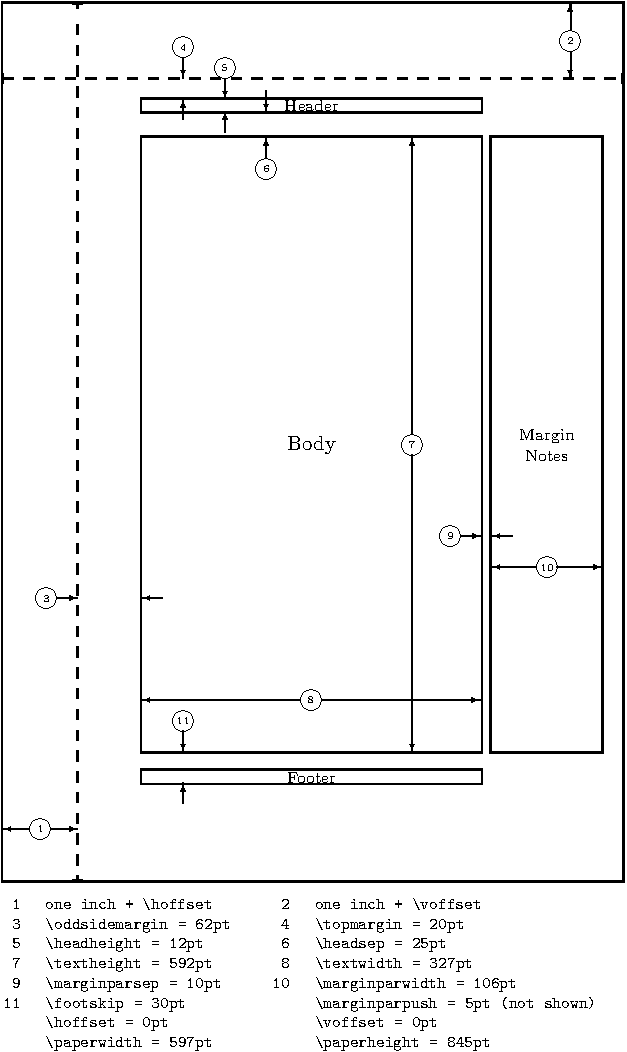
\includegraphics[width=.8\textwidth]{images/mylayout}
  \caption{版面のレイアウトに使用できる長さ}\figlab{pagelayout}
 \end{center}
\end{figure}
\indindz{ファイル}{クラス}%
このような版面を視覚的に確認するには\Y{layout}パ
ッケージが使えます.このパッケージは使用されている%
クラスファイルから版面のレイアウトを出力します.
使用方法は\env{document}環境中で \C{layout} 命令を
使うだけです.

\begin{Prob}
\Y{layout}パッケージを使って,特定のクラスファイルの標準的
なページレイアウトがどのようになっているかを,次のような
ファイルをタイプセットする事により確認してください.

\begin{InTeX}
\documentclass{jsarticle}
\usepackage{layout}
\begin{document}
\layout
\end{document}
\end{InTeX}

\cls{jsarticle}以外にも \Cls{jsbook} や \Cls{jbook} 等でも
確認してみてください.
\end{Prob}


\index{用紙}
まずはページ全体の\Z{余白}に関する長さです.\zindind{ページ}{の余白}
\begin{description}
 \item[\Cmd{voffset}] \zindind{用紙}{の空白}
 横組みにおいて用紙の左上の部分に入れる縦方向の余白.
 この値を0にしてもすでに1インチ分の余白が挿入されています.
 本当に用紙の左上端から使うならば \cmd{voffset}を
 \qu{\str{-1in}}に設定します.

 \item[\Cmd{hoffset}] 
 横組みにおいて用紙の左上の部分に入れる横方向の余白.
 縦方向と同じようにすでに1インチ分の余白が挿入されています.

 \item[\Cmd{oddsidemargin}]
ページが奇数のときに挿入される左側の余白.
文書クラスオプションに\Option{oneside}を
使っていると全てのページに \cmd{oddsidemargin}が
挿入されます.

 \item[\Cmd{evensidemargin}] 
ページが偶数のときに挿入される左側の余白.
文書クラスオプションに\Option{twoside}を
使っているときだけ有効で\Option{oneside}では
意味がありません.
\end{description}

ヘッダの設定に関する長さです.
\begin{description}
\item[\Cmd{topmargin}] 
\cmd{voffset}とヘッダの間隔です.
\item[\Cmd{headheight}]
ヘッダの高さです.\indindz{高さ}{ヘッダの}%
\item[\Cmd{headsep}]
ヘッダと本文領域の間隔です.
\item[\Cmd{footskip}]
フッタ下部と本文領域の最下部との間隔です.
\end{description}

本文領域や傍注領域に関わる長さです.
\begin{description}
\item[\Cmd{textheight}]\indindz{高さ}{本文領域の}%
 本文領域の高さです.ヘッダやフッタの高さは含まれません.
 \item[\Cmd{textwidth}]
 本文領域の幅です.\indindz{幅}{本文の}%
 \item[\Cmd{marginparwidth}]
  傍注の幅です.\indindz{幅}{傍注の}%
 \item[\Cmd{marginparpush}]
 傍注と傍注のあいだの縦方向の長さです.
 \item[\Cmd{marginparsep}]
 傍注と本文領域との間隔です.
 \item[\Cmd{columnsep}]
 2段組以上での段と段の間隔です.
 \item[\Cmd{columnseprule}]
 2段組以上での段と段のあいだに入る罫線です.\indindz{罫線}{2段組での}
\end{description}
通常ここで紹介した長さはクラスファイル側
でフォントサイズやクラスオプションに応じ
て適切に設定されますので徒に変更しないでください.\zindind{ページ}{の行数}
相手先の都合で\yo{1行何文字1ページ何行}
のような設定などをしなければならないときは無理やり
次のようにする事もできます.

\begin{InTeX}
\setlength{\textwidth}{33zw}
\setlength{\textheight}{40\baselineskip}
\end{InTeX}



\subsection{簡単なページレイアウト\zdash \Y{geometry}}
\zindind{版面}{の設定}%
\indindz{余白}{上下左右の}%

例えば,「上下左右の余白を 2\,cm とし,残りの領域は本文に使い,
\Z{フッター}と\Z{ヘッダー}は本文の領域の高さに含める」という
ページレイアウトにしたければ,大雑把には次のような設定をする
事になります.
\begin{eqnarray*}
 \begin{aligned}
 \cmd{voffset}        & = -0.54\,\mathrm{cm} \\
 \cmd{hoffset}        & = -0.54\,\mathrm{cm} \\
 \cmd{evensidemargin} & = 0\,\mathrm{cm} \\ 
 \cmd{ossdidemargin}  & = 0\,\mathrm{cm} \\
 \cmd{textheight} 
   & = \cmd{paperheight} - 4\,\mathrm{cm} - \cmd{topmargin} \\
   & - \cmd{headheight} - \cmd{headsep} - \cmd{footskip}  \\
 \cmd{textwidth}   & = \cmd{paperwidth} - 4\,\mathrm{cm}  
 \end{aligned}
\end{eqnarray*}
これにより,\LaTeX では次のような設定をする事になります.

\begin{InTeX}
\setlength   \voffset        {-1in}% \voffset の設定
\addtolength \voffset        {2cm}
\setlength   \hoffset        {-1in}% \hoffset の設定
\addtolength \hoffset        {2cm}
\setlength   \textheight     {\paperheight}% \textheight の設定
\addtolength \textheight     {-4cm}
\addtolength \textheight     {-\topmargin}
\addtolength \textheight     {-\headheight}
\addtolength \textheight     {-\headsep}
\addtolength \textheight     {-\footskip}
\setlength   \textwidth      {\paperwidth}% \textwidth の設定
\addtolength \textwidth      {-4cm}
\setlength   \evensidemargin {0pt}% 偶数ページマージン
\setlength   \oddsidemargin  {\evensidemargin}% 奇数ページマージン
\setlength   \fullwidth      {\textwidth} 
\end{InTeX}

\indindz{印刷}{両面}%
しかし,\Z{両面印刷}をするとか,ヘッダーやフッターの高さを含む等の
調整が絡んでくると,少々入り組んだ設定になってしまいます.
そこで,もう少し簡単に版面の設定をしたいならば\Hito{梅木}{秀雄}
の作成した\sty{geometry}を使うのが良いでしょう.\Y{geometry}
パッケージは非常に多機能で,その全てを本書で紹介する事はできません
が,初学者がもっとも苦労し,様々な問題に直面する事が多いように見受けら
れますので,なるべく詳細に解説します.

使い方は非常に簡単で,プリアンブルで\Y{geometry}パッケージをオプション付
きで読み込むだけです.

\begin{InTeX}
\usepackage[margin=2cm]{geometry}
\end{InTeX}

上記のようにすると文章領域の上下左右の余白を 2\,cm に設定します
\footnote{用紙にはヘッダ,フッタ,傍注がありますから,これらの領域を除い
た文面の余白が 2\,cmという事になります.}.

他には \Y{geometry} パッケージを読み込んだ後に \C{geometry} コマンドを
使う方法です.これはプリアンブルのみで使う事ができます.

\begin{InTeX}
\usepackage[a5paper]{geometry} 
\geometry{hmargin={3cm,0.8in},height=8in}
\geometry{height=10in}
\end{InTeX}

\Y{geometry}パッケージは\Y{calc}パッケージにも対応していますので,
次のような記述も可能です.

\begin{InTeX}
\usepackage{calc}
\usepackage[textheight=20\baselineskip+10pt]{geometry}
\end{InTeX}

\Y{jsclasses}に含まれる,\Cls{jsbook}クラスを用いている場合
は \C{fullwidth} を \C{textwidth} に設定するのが良い時があります.

\begin{InTeX}
\setlength \fullwidth{\textwidth}
\end{InTeX}

以下に\Y{geometry}のパッケージオプションを挙げます.
パッケージオプションは基本的には \C{geometry} 命令の中で使うことができま
す.

\newcommand*\twoargs[2]{\texttt{\lb}\va{#1}\str,\va{#2}\texttt{\rb}}
\newcommand*\threeargs[3]{\texttt{\lb}\va{#1}\str,\va{#2}%
  \str,\va{#3}\texttt{\rb}}

\paragraph{用紙サイズ}

\begin{description}
 \item[既定のサイズ]
\zindind{用紙}{の既定のサイズ}
  \Optionlist{a0paper,a1paper,a2paper,a3paper,a4paper,a5paper,a6paper,%
  b0paper,b1paper,b2paper,b3paper,b4paper,b5paper,b6paper,%
  letterpaper,executivepaper,legalpaper,screen}.
  \option{screen} は 225\,mm $\times$ 180\,mm になります.
  \option{screen}は\option{centering} も併用すると便利です.
  `\str{paper=}\va{用紙サイズ}'と記述しても大丈夫です.
\item[\Option{paperwidth}] 
\zindind{用紙}{の幅}
  \Z{用紙}の幅を,\va{長さ}を指定して決めます.
  `\str{paperwidth=10cm}'のように使います.
\item[\Option{paperheight}]
\zindind{用紙}{の高さ}
  用紙の高さを,\va{長さ}を指定して決めます.
\item[\Option{papersize}]
  `\option{papersize}\str=\twoargs{幅}{高さ}'とするか,
  `\option{papersize}\str=\va{長さ}'とすれば \option{paperwidth}
  と\option{paperheight}を用いた事と等価になります.
\item[\Option{landscape}] 
  \Z{横置き}でページレイアウトを設定します.
\item[\Option{portrait}]
  \Z{縦置き}でページレイアウトを設定します.
\end{description}

\paragraph{本文のパラメータ}

\begin{description}
 \item[\Option{hscale}] 
  用紙の幅 (\C{paperwidth}) に対して本文領域が占める横幅の比率です.
  `\str{hscale=.8}' とすると `\str{width=.8\bs paperwidth}' と等価になりま
  す.標準は 0.7 です.
 \item[\Option{vscale}] 
  用紙の高さ (\C{paperheight}) に対して本文領域が占める高さの比率です.
  `\str{vscale=.8}' とすると `\str{height=.9\bs paperheight}' と等価になりま
  す.標準は 0.7 です.
 \item[\Option{scale}] 
  本文が幅と高さに関して用紙に対して占める比率を指定します.
  `\str{scale=}\twoargs{幅の比率}{高さの比率}'
   とするか`\str{scale=}\va{比率}'として使います.標準は 0.7 です.
 \item[\Option{width}/\Option{totalwidth}] 
\indindz{幅}{本文のトータルな}
  本文のトータルな幅を指定します.`\str{width=}\va{長さ}'とするか,
  `\str{totalwidth=}\va{長さ}'とします.
 \item[\Option{height}/\Option{totalheight}] 
\indindz{高さ}{本文のトータルな}
  本文のトータルな高さを指定します.`\str{height=}\va{長さ}'とするか,
  `\str{totalheight=}\va{長さ}'とします.
 \item[\Option{total}] 
  本文のトータルな幅と高さを指定します.
  `\str{total=}\twoargs{幅}{高さ}'とするか,
  `\str{total=}\va{長さ}'とします.
 \item[\Option{textwidth}] 
   文章領域となる \C{textwidth} の幅を指定します.
   `\str{textwidth=}\va{長さ}'とします.
 \item[\Option{textheight}]
   文章領域となる \C{textheight} の高さを指定します.
   `\str{textheight=}\va{長さ}'とします.
 \item[\Option{text}/\Option{body}]
  \C{textwidth} と \C{textheight} の両方を指定します.
  `\str{body=}\twoargs{幅}{高さ}'とするか`\str{text=}\va{長さ}'とします.
 \item[\Option{lines}]
  \cmd{textheight} を\Z{行数}によって決めます.`\str{lines=}\va{整数}'で指定
  します.
 \item[\Option{includehead}]
  トータルな本文の高さ\option{height}/\option{totalheight}にヘッダー
  (\C{headheight} と \C{headsep}) を含めるようにします.標準では無効です.
 \item[\Option{includefoot}]
  トータルな本文の高さ\option{height}/\option{totalheight}にフッター
  (\C{footskip}) を含めるようにします.標準では無効です.
 \item[\Option{includeheadfoot}]
  \option{includehead} と \option{includefoot} の両方を有効にします.
 \item[\Option{includemp}]
  トータルな本文の幅に\Z{傍注} (\C{marginparwidth} と \C{marginparsep}) も
  含めるようにします.\Option{marginparwidth}と\Option{marginparsep}オプ
  ションに依存しています.標準では無効です.
 \item[\Option{includeall}]
  \option{includeheadfoot} と \option{includemp} の両方を指定した事と等
  価です.
 \item[\Option{ignorehead}]
  トータルな本文の高さにヘッダーを含めないようにします.標準で有効です.
  `\str{includehead=false}'とするのと等価です.
 \item[\Option{ignorefoot}]
  トータルな本文の高さにフッターを含めないようにします.標準で有効です.
  `\str{includefoot=false}'とするのと等価です.
 \item[\Option{ignoreheadfoot}]
  \option{ignorehead} と \option{ignorefoot} の両方を指定した事と等価で
  す.
 \item[\Option{ignoremp}]
  トータルな本文の幅に傍注を含めないようにします.標準で有効です.
 \item[\Option{ignoreall}]
  \option{ignoreheadfoot} と \option{ignoremp} の両方を指定した事と等価
  です.
 \item[\Option{heightrounded}]
  本文の高さが行送りの倍数でない場合に,``\str{underfull vbox}''の警告を
  出さないように \C{textheight} を \va{\C{baselineskip} の整数倍 $+$
  \C{topskip}} にします.
 \item[\Option{hdivide}]
  左余白,文章の幅,右余白を指定します.`\str{hdivide=}%
  \threeargs{左余白}{文章幅}{右余白}'のように使います.
  このオプションは三つのうち二つだけ明確な時に,不定の一つを星`\str{*}'
  に置き換えて`\str{hdivide=\lb2cm,15cm,*\rb}'とできます.
 \item[\Option{vdivide}]
  \Z{上余白},文章の高さ,\Z{下余白}を指定します.`\str{vdivide=}%
  \threeargs{上余白}{文章幅}{下余白}'のように使います.
 \item[\Option{divide}]
  `\str{divide=}\threeargs{長さ\mbox{$_1$}}{長さ\mbox{$_2$}}{長さ
  \mbox{$_3$}}'とすると`\str{hdivide=}\threeargs{長さ\mbox{$_1$}}{長さ
  \mbox{$_2$}}{長さ\mbox{$_3$}}'と\str{vdivide=}\threeargs{長さ
  \mbox{$_1$}}{長さ\mbox{$_2$}}{長さ\mbox{$_3$}}'を指定した事と等価にな
  ります.
\end{description}

\paragraph{余白}

\begin{description}
 \item[\Option{left}/\Option{lmargin}/\Option{inner}]
 \zindind{用紙}{の左端}
 用紙の左端と本文領域(版面)とのあいだにある左余白を指定します.
 `\str{lmargin=}\va{長さ}'のように使います.両面印刷指定
 (\Option{twoside}) の場合は\Z{ノド}の長さを設定します.
 \item[\Option{right}/\Option{rmargin}/\Option{outer}]
 \zindind{用紙}{の右端}
 用紙の右端と本文領域とのあいだにある右余白を指定します.
 `\str{rmargin=}\va{長さ}'のように使います.両面印刷指定
 (\Option{twoside}) の場合は\Z{小口}の長さを設定します.
 \item[\Option{top}/\Option{tmargin}]
  用紙の上端と本文領域のとのあいだ(\Z{天})にある上余白を指定します.
 `\str{tmargin=}\va{長さ}'のように使います.
 \item[\Option{bottom}/\Option{bmargin}]
  用紙の下端と本文領域のとのあいだ(\Z{地})にある下余白を指定します.
 `\str{bmargin=}\va{長さ}'のように使います.
 \item[\Option{hmargin}]
  左右余白を指定します.`\str{hmargin=}\twoargs{左余白}{右余白}'とするか,
  `\str{hmargin=}\va{長さ}'とします.
 \item[\Option{vmargin}]
  上下余白を指定します.`\str{vmargin=}\twoargs{上余白}{下余白}'とするか,
  `\str{vmargin=}\va{長さ}'とします.
 \item[\Option{margin}]
  `\str{margin=}\twoargs{長さ\mbox{$_1$}}{長さ\mbox{$_2$}}'とすると,
  `\str{hmargin=}\twoargs{長さ\mbox{$_1$}}{長さ\mbox{$_2$}}'と
  `\str{vmargin=}\twoargs{長さ\mbox{$_1$}}{長さ\mbox{$_2$}}'を指定した
  事と等価になります.
 \item[\Option{hmarginratio}]
  左右余白の比率を指定します.`\str{hmarginration=}\va{左の比率\str:右の比率}'
  のようにコロンで区切ります.正の整数値で 100 以下である必要があります.
  片面印刷時 (\Option{oneside}) は $1:1$, 両面印刷時 (\Option{twoside})
  は $2:3$ が標準です.
  \item[\Option{vmarginratio}]
  用紙の上余白と下余白(\Z{天地})の比率を指定します.
 \item[\Option{marginratio}]
  `\str{marginratio=}\twoargs{左右の比率}{上下の比率}'とするか,
  `\str{marginration=}\va{比率}'とします.
 \item[\Option{hcentering}]
  `\str{hmarginration=1:1}'とした事と等価になります.
 \item[\Option{vcentering}]
  `\str{vmarginration=1:1}'とした事と等価になります.
 \item[\Option{centering}]
  `\str{marginration=1:1}'とした事と等価になります.
 \item[\Option{twoside}]
 \zindind{左右}{対称}
  \Z{両面印刷}時に文章領域(\Z{版面})が左右対称になるようにします.
 \item[\Option{asymmetric}]
 \zindind{左右}{非対称}
  両面印刷時に文章領域が左右非対称になるようにします.ただし,
  \option{bindingoffset}は考慮されます.
 \item[\Option{bindingoffset}]
  \zindind{文書}{を綴じる}
  \Z{片面印刷}時でも両面印刷時においても文書を綴じる背の部分の余白を
  指定します.`\str{bindingoffset=}\va{長さ}'として使います.
\end{description}

\paragraph{レイアウトパラメータの設定}

\LaTeX のページレイアウトにおけるパラメータを設定する事もできます.
%the options below specify \LaTeX\ native dimension and switches for page
%layout. See Figure~1. Note that unlike version~2.3, \option{nohead},
%\option{nofoot} and \option{noheadfoot} become overwritable, in other
%words, just shorthand for setting the corresponding \LaTeX\ dimensions
%(\cmd{headheight}, \cmd{headsep}, \cmd{footskip}) to 0\,pt.

\begin{description}
 \item[\Option{headheight}/\Option{head}] 
  `\str{head=}\va{長さ}'として \C{headheight} を設定します.
 \item[\Option{headsep}] 
  `\str{headsep=}\va{長さ}'として \C{headsep} を設定します.
 \item[\Option{footskip}/\Option{foot}] 
  `\str{foot=}\va{長さ}'として \C{footskip} を設定します.
 \item[\Option{nohead}] 
  ヘッダー無しの設定にします(\C{headheight} と \C{headsep} を 0\,pt
  にします).
 \item[\Option{nofoot}] 
  フッター無しの設定にします(\C{footskip} を 0\,ptにします).
 \item[\Option{noheadfoot}] 
  \option{nohead} と \option{nofoot} を指定した事と等価になります.
 \item[\Option{marginparwidth}/\Option{marginpar}] 
 \zindind{傍注}{の幅}
  `\str{marginpar=}\va{長さ}'として傍注の幅 \C{marginparwidth} を設定し
  ます.
 \item[\Option{marginparsep}]
 \zindind{傍注}{と本文の空き}
  `\str{marginparsep=}\va{長さ}'として傍注と本文の空き \C{marginparsep}
  を設定します. 
 \item[\Option{nomarginpar}]
  傍注無しの設定にします(\C{marginparwidth} と \C{marginparsep} を
  0\,pt にします).
 \item[\Option{columnsep}]
  `\str{columnsep=}\va{長さ}'として\Z{段間}の空き \C{columnsep} を設定します.
 \item[\Option{hoffset}]
  `\str{hoffset=}\va{長さ}'として \C{hoffset} を設定します.
 \item[\Option{voffset}]
  `\str{voffset=}\va{長さ}'として \C{voffset} を設定します.
 \item[\Option{offset}]
  `\str{offset=}\twoargs{水平方向のオフセット量}{垂直方向のオフセット量}'と
  するか`\str{offset=}\va{オフセット量}'として,\Z{オフセット}を指定します.
 \item[\Option{twocolumn}]
  2段組の設定にします.
 \item[\Option{twoside}]
  両面印刷用に傍注の位置を入れ換え,紙面を左右対称になるようにします.
 \item[\Option{textwidth}]
  `\str{textwidth=}\va{長さ}'として \C{textwidth} を直接指定します.
 \item[\Option{textheight}]
  `\str{textheight=}\va{長さ}'として \C{textheight} を直接指定します.
 \item[\Option{reversemp}/\Option{reversemarginpar}]
 傍注の位置を非標準の左側に出力するようにします.両面印刷時は
 \Z{見開き}の内側(小口)に設定します.
\end{description}

\paragraph{デバイスドライバ}

\begin{description}
 \item[\Option{dvips}] \Prog{dvips}用に用紙サイズ情報を設定します.
 \item[\Option{dvipdfm}] \Prog[dvipdfm]{\Dvipdfm}用に用紙サイズ情報を設
 定します.
 \item[\Option{pdftex}] \Prog[pdftex]{\PDFTeX},
 \Prog[pdflatex]{\PDFLaTeX}用に用紙サイズ情報を設定します.
\end{description}

\paragraph{その他}

\begin{description}
 \item[\Option{verbose}] 
  \Y{geometry}パッケージの処理内容を詳細に表示します.
 \item[\Option{showframe}] 
  ページレイアウトの設定を確認するために,1ページ目の本文領域,ヘッダー,
  フッターを枠で囲みます.
% \item[\Option{reset}] 
% \item[\Option{mag}] 
% \item[\Option{truedimen}] 
% \item[\Option{pass}] 
% \item[\Option{compat2}] 
\end{description}

\makeatletter
\newcommand*\geoimage[2][clip]{%
  \noindent
  \hbox{\includegraphics[scale=1,#1]{geolay/geo#2-2-crop.pdf}}%
  \nobreakspace
  \hbox{\includegraphics[scale=1,#1]{geolay/geo#2-1-crop.pdf}}%
}
\newcommand*\GQ{,}
\newcommand\geooptionlist[1]{
 \@for\member:=#1\do{\advance\@tempcnta\@ne}%
 \@for\member:=#1\do{\advance\@tempcntb\@ne
   \ifnum\@tempcntb<\@tempcnta
         \texttt{\member},\\
 \else
  \ifnum\@tempcntb=\@tempcnta
    \texttt{\member}%
  \fi
\fi}%
}
%\newcommand*\GeoOptions[2][7em]{%\geooptionlist{#1}%
% \fbox{\parbox[b]{#1}{\geooptionlist{#2}}}%
%}
\newcommand\GEO[5][\geoimage]{%
\par\vskip.5\cvs
\noindent\makebox[0pt][l]{%
   {\begin{minipage}[c]{#4\fullwidth}%
      \small \geooptionlist{#2}%
   \end{minipage}}%
   \hfil
   {%
    \begin{minipage}{#5\fullwidth}%
     \null\hfill #1{#3}%
   \end{minipage}%
   }%
}\par\vskip.5\cvs
}

\makeatother

\Cls{jsbook}クラスでのレイアウト例を示します.まずパッケージを読み込まな
い状態でのレイアウトです.

\GEO{パッケージ無し}{1}{.2}{.8}

\begin{Prob}
上下左右の余白をちょうど 2\,cm に設定するにはどうすれば良いか
考えてください.%少なくとも解は一つ以上あります.
%\GEO{margin=2cm}{2}{.2}{.8}
この場合はヘッダー,フッター,傍注の領域が含まれない事も確認してください.
\end{Prob}

次は上下の余白の比率を $1:1$,左右の余白の比率を $1:1$ に
指定した例です.

\GEO{centering}{3}{.2}{.8}

この場合もヘッダー,フッター,傍注の領域は含まれません.
次は見開きの内側の余白を 1\,cm足した例です.

\GEO{twoside,bindingoffset=1cm}{4}{.2}{.8}

\begin{Prob}
左余白を 3\,cm,右余白を 2\,cm,\Z{行数}を40行送り分,上余白を
2.5\,cmとして,ヘッダーとフッターの領域をトータルな高さに含める
ような \Y{geometry} の設定を考えてください.いくつも解答はありますが,
例えば次のような設定の実行結果を吟味してください.

\begin{InTeX}
\geometry{left=3cm,right=2cm,lines=40,top=2.5cm,includeheadfoot}
\end{InTeX}
%\GEO{left=3cm,right=2cm,lines=40,top=2.5cm,includeheadfoot}{5}{.2}{.8}

また,これは次のようにしても同じである事を確認してください.

\begin{InTeX}
\geometry{hmargin={3cm,2cm},tmargin=2.5cm,lines=40,includeheadfoot}
\end{InTeX}
\end{Prob}

%\GEO{hmargin=\lb3cm\GQ2cm\rb,tmargin=2.5cm,lines=40,includeheadfoot}{6}

次は本文の高さを 10\,inch,下余白を 2\,cm,残りは上余白にするような
設定です.

\GEO{vdivide=\\\lb*\GQ10in\GQ2cm\rb}{7}{.2}{.8}

これは次のようにしても同じ事になります.

\begin{InTeX}
\geometry{bottom=2cm,textheight=10in}
\end{InTeX}

%\GEO{bottom=2cm,textheight=10in,includefoot}{8}

次は幅も高さも用紙の 80\% だけ本文の領域に割り当てるようにし,
用紙の中央に本文が配置するようにします.

\GEO{scale=0.8,centering}{9}{.2}{.8}

用紙サイズを A5 とし,傍注の幅を 3\,cm,傍注の幅もトータルな幅に含めるよ
うにします.

\GEO{a5paper,marginparwidth=3cm,includemp}{10}{.3}{.7}

次は用紙サイズを B4 とし,横置き,2段組,左右上下の余白は2\,cm,
傍注・ヘッダー・フッターなしで,段間の幅を 2\,cm とします.

\GEO[\includegraphics]{dvipdfm,b4paper,landscape,twocolumn,margin=2cm,nomarginpar,nofoot,nohead,columnsep=2zw}{geolay/geo11-1-crop.pdf}{.2}{.8}
%\hbox{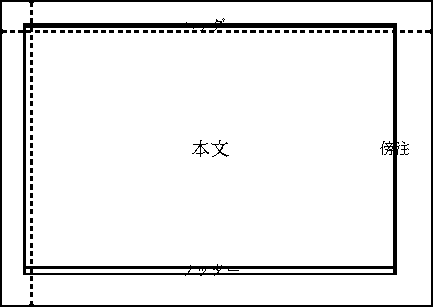
\includegraphics[scale=1]{geolay/geo11-1-crop.pdf}}%

%  vmargin=25mm,hmargin=15mm,
%  tmargin=25mm,bmargin=25mm,lmargin=15mm,rmargin=15mm,
%  top=25mm,bottom=25mm,left=15mm,right=15mm,

次は用紙サイズを A4 として,2段組,左右余白をそれぞれ 15\,mm,
上下余白を 25\,mm,段間の幅を 6\,mm,傍注・ヘッダー・フッター
なしの設定にします.

\GEO[\includegraphics]{a4paper,twocolumn,ignoreall,nomarginpar,noheadfoot,margin=\lb15mm\GQ25mm\rb,columnsep=6mm}{geolay/geo12-1-crop.pdf}{.3}{.7}
%\hbox{[scale=1]{geolay/geo12-1-crop.pdf}}%


%\endinput


\subsection{ヘッダやフッタの設定その1}\indindz{番号}{ページ}%
ヘッダやフッタなどに出力されるページ番号などを\zindind{ページ}{の番号}
変更したいときがあると思います.
\begin{Syntax}
\C{pagestyle}\pa{表示形式}
\end{Syntax}

\C{pagestyle}命令を記述したページから指定した\Z{表示形式}に変更されま
す.指定できる形式は\tabref{pagestyle}の通りです.


\begin{table}[htbp]
\begin{center}
\caption{ヘッダやフッタの指定}\tablab{pagestyle}
\begin{tabular}{ll}
\TR
\Th{命令}        & \Th{内容} \\
\MR
\str{empty}      & ページ番号を表示しない                \\
\str{plain}      & フッタ中央部に表示する              \\
\str{headings}   & ヘッダにページ番号と章・節名を表示する\\
\str{myheadings} & ユーザ定義の表示形式にする          \\
\BR
\end{tabular}
\end{center}
\end{table}

\qu{\str{myheadings}}では二つの命令によってヘッダの出力を指定します.

\begin{Syntax}
\Cmd{markright} \pa{ヘッダ} \\
\Cmd{markboth} \pa{偶数ヘッダ}\pa{奇数ヘッダ}
\end{Syntax}


片面印刷のときに \cmd{markright}を使います.
両面印刷には \Cmd{markboth}を使います.
2006年度版の\yo{○○△△大学}の論文集を
作成しているのであれば,例えば次のようにします.

\begin{InTeX}
\pagestyle{myheadings}
\markboth{○○△△大学論文集}{2006年度版}
\end{InTeX}


任意の1ページだけのヘッダ・フッタは,
次のようにする事でそのページだけ変えられます.

\begin{Syntax}
\Cmd{thispagestyle}\pa{表示形式}
\end{Syntax}


ページ番号の表示形式を変更するには \C{pagenumbering}命令を使います.

\begin{Syntax}
\Cmd{pagenumbering}\pa{表示形式}
\end{Syntax}

その場所から指定した形式で1ページ目からカウントしてページ番号を表示しま
す.指定できる表示形式は\tabref{pagenumber}の通りです.

\begin{table}[htbp]
\begin{center}
\caption{ページ番号の種類の指定}\tablab{pagenumber}
\begin{tabular}{lll}
\TR
\Th{形式}          & \Th{内容}          & \Th{出力例}         \\
\MR
\verb+arabic+ & \Z{アラビア数字}       & 1, 2, 3,\,\ldots \\
\verb+roan+   & \Z{ローマ数字}   & i, ii, iii,\,\ldots\\
\verb+Roman+  & ローマ数字   & I, II, III,\,\ldots\\
\verb+alph+   & アルファベット小文字& a, b, c,\,\ldots,\, z\\
\verb+Alph+   & アルファベット大文字& A, B, C,\,\ldots,\, Z\\
\BR
\end{tabular}
\end{center}
\end{table}
ここで注意する事はアルファベットにした場合は,
最大26ページまでしかカウントできないという事
です.27以上になった場合の対策は別にする事に
なります.

%もっと詳細なヘッダ・フッタ定義するときは自分で
%\cmd{ps@なんとか}というコマンドを定義してこれを
%\begin{InTeX}
%pagestyle{なんとか} 
%\end{InTeX}
%のように使います.本書で使われているスタイルは
%以下の通りです.\hito{奥村}{晴彦}の\cls{jsclasses}
%を少し変更しただけです.
%\begin{InTeX}
%\newcommand{\ps@myhead}{%
%  \let\@oddfoot\@empty
%  \let\@evenfoot\@empty
%  \def\@evenhead{%
%    \if@mparswitch \hss \fi
%    \underline{\hbox to \fullwidth{\autoxspacing
%        \textbf{\thepage}\hskip3zw\leftmark\hfill\@title}}%
%    \if@mparswitch\else \hss \fi}%
%  \def\@oddhead{\underline{\hbox to \fullwidth{\autoxspacing
%        \@title\hfill{\if@twoside\rightmark\else\leftmark\fi}%
%	\hskip3zw\textbf{\thepage}}}\hss}%
%  \let\@mkboth\markboth
%  \def\chaptermark##1{\markboth{%
%    \ifnum \c@secnumdepth >\m@ne
%      \if@mainmatter
%        \@chapapp\thechapter\@chappos\hskip1zw
%      \fi
%    \fi
%    ##1}{}}%
%  \def\sectionmark##1{\markright{%
%    \ifnum \c@secnumdepth >\z@ \thesection \hskip1zw\fi
%    ##1}}}%
%\end{InTeX}
%これを別ファイル\fl{hoge.sty}などにまとめて\cmd{usepackage}
%するか,\cmd{makeatletter}と\cmd{makeatother}で囲むかで
%実際の出力を確認してみてください.


\subsection{ヘッダ・フッタの変更その2\zdash\Y{fancyhdr}}
\indindz{スタイル}{ページ}%
\zindind{ページ}{スタイル}%
{\LaTeX}が標準で用意してくれているページスタイル
では寂しい,そう思う人も多いでしょう.自分で全て
定義する事もできますが,\Person{Piet}{Oostrum}が
作成した \Y{fancyhdr} を使うと比較的簡単にペー
ジスタイルをカスタマイズできます.\sty{fancyhdr}
は\Sty{fancyheadings}の後継で,ページのヘッダーと
フッターをカスタマイズできるマクロです.
まず\sty{fancyhdr}を使うために以下をプリアンブルに記述します.

\begin{InTeX}
\usepackage{fancyhdr} 
\pagestyle{fancy}
\end{InTeX}

\sty{fancyhdr}では
ヘッダ・フッタを六つに分割しています.
\begin{center}
\begin{tabularx}{\linewidth}{|XcX|}
\hline
\cmd{lhead} & \cmd{chead} & \hfill\cmd{rhead}\\
\multicolumn{3}{|c|}{%
   \hrulefill \pp{\cmd{headrulewidth}}\hrulefill} \\   
\multicolumn{3}{|c|}{\va{本文領域}}\\
\multicolumn{3}{|c|}{%
   \hrulefill \pp{\cmd{footrulewidth}}\hrulefill} \\
\cmd{lfoot} & \cmd{cfoot} &\hfill\cmd{rfoot} \\
\hline
\end{tabularx}
\end{center}
\Cmd{lhead},\Cmd{chead},\Cmd{rhead}の
三つはヘッダに使い\Cmd{lfoot},\Cmd{cfoot},
\Cmd{rfoot}の三つはフッタに使います.%
\indindz{罫線}{ヘッダ上部の}\indindz{罫線}{フッタ上部の}%%
\Cmd{headrulewidth}はヘッダ下部の罫線の太さで,
\Cmd{footrulewidth}はフッタ上部の罫線の太さです.
図だけのページや表だけのページはシンプルな
ヘッダ・フッタにしたり,ヘッダ下部の罫線を
引かない場合があります.その場合は \C{headrulewidth} を
\C{iffloatpage}命令で判定するように定義すると良いでしょう.

\begin{InTeX}
\def\headrulewidth{\iffloatpage{0pt}{.4pt}} 
\end{InTeX}

\cmd{lhead}などの
他の命令も同様に変更できます.

例えば\cls{jarticle}クラスで次のようなヘッダ・フッタ
\begin{center}
\begin{tabularx}{\linewidth}{|cXcXc|}
\hline
& & \hskip5em & \hfill 資本主義社会の崩壊 & \\
\cline{2-4}
\multicolumn{5}{|c|}{\va{本文領域}}\\
\cline{2-4}
& 名無しの権兵衛 & \hskip3em & \hfill \textbf{ページ番号} & \\
\hline
\end{tabularx}
\end{center}
を設定したければ以下のように記述します.

\begin{InTeX}
\lhead{} \chead{}
\rhead{資本主義社会の崩壊}
\lfoot{名無しの権兵衛} 
\cfoot{}
\rfoot{\textbf{\thepage}}
\def\headrulewidth{.4pt}
\def\footrulewidth{.4pt}
\end{InTeX}

書籍用クラス\cls{jbook}などでクラスオプションに
\Option{twoside}が指定されている場合は偶数ページと
奇数ページを個々に設定します.例えば次のような
ヘッダ・フッタにしたいとします.
\begin{center}
\begin{tabular}{|p{7zw}cp{7zw}|}
\hline
第1章\hskip1zw 序論& & \hfill 1.1\hskip1zw 背景\\\hline
\multicolumn{3}{|c|}{本文}\\\hline
& \textbf{2}&\hfill \\\hline
\end{tabular} \hfill
\begin{tabular}{|p{7zw}cp{7zw}|}
\hline
1.2\hskip1zw  目標& & \hfill 第1章\hskip1zw 序論\\\hline
\multicolumn{3}{|c|}{本文}\\\hline
& \textbf{3}& \\\hline
\end{tabular}
\end{center}
ヘッダ・フッタの奇数ページと偶数ページの場所
を区別するために以下のような設定になっています.
\begin{center}
\begin{tabular}{|p{6zw}cp{6zw}|}
\hline
\str{EL(H)}& \str{EC(H)}& \hfill  \str{ER(H)}\\\hline
\multicolumn{3}{|c|}{本文}\\\hline
\str{EL(F)}& \str{EC(F)} &\hfill \str{ER(F)} \\\hline
\multicolumn{3}{c}{偶数ページ側}\\
\end{tabular} \hfill
\begin{tabular}{|p{6zw}cp{6zw}|}
\hline
\str{OL(H)} &\str{OC(H)} & \hfill \str{OR(H)} \\\hline
\multicolumn{3}{|c|}{本文}\\\hline
\str{OL(F)}&\str{OC(F)} & \hfill  \str{OR(F)}\\\hline
\multicolumn{3}{c}{奇数ページ側}\\
\end{tabular}
\end{center}
先程の出力を得るためには \Cmd{fancyhead} と \Cmd{fancyfoot}命令を使います.

\begin{InTeX}
\documentclass{jbook}
\usepackage{fancyhdr} \pagestyle{fancy}
\fancyhead[ER,OL]{\rightmark}
\fancyhead[EL,OR]{\leftmark}
\fancyfoot[EC,OC]{\textbf{\thepage}}
\end{InTeX}

欧文のクラスではこれで良いのですが和文では \Cmd{chaptermark} と 
\Cmd{sectionmark}の定義を\sty{fancyhdr}を読み込んだ後に次のように定義
するのが普通でしょう.

\begin{InTeX}
 \def\chaptermark#1{\markboth{%
   \ifnum \c@secnumdepth >\m@ne
     \if@mainmatter
       \@chapapp\thechapter\@chappos\hskip1zw
     \fi
   \fi
   #1}{}}%
  \def\sectionmark#1{\markright{%
    \ifnum \c@secnumdepth >\z@ \thesection \hskip1zw\fi
    #1}}%
\end{InTeX}


\subsection{ページ/総ページ}

ヘッダ・フッタの設定をフッタだけに\yo{ページ/総ページ}にしたい場合がある
でしょう.これは例えば次のようにプリアンブルに記述します.

\C*{AtEndDocument}%
\C*{ps@total}%
\C*{@mkboth}%
\C*{@gobbletwo}%
\C*{@oddhead}%
\C*{@empty}%
\C*{@evenhead}%
\C*{@evenhead}%
\C*{@oddfoot}%
\C*{normalfont}%
\C*{thepage}%
\C*{hfil}%
\C*{@evenfoot}%
\begin{InTeX}
\AtEndDocument{\label{lastpage}}
\makeatletter
 \newcommand{\ps@total}{%
 \let\@mkboth\@gobbletwo
 \let\@oddhead\@empty
 \let\@evenhead\@empty
 \def\@oddfoot{\normalfont\hfil--\thepage/\pageref{lastpage}--\hfil}%
 \let\@evenfoot\@oddfoot}
\makeatother
\pagestyle{total}
\end{InTeX}

この場合は \cmd{ps@total}によって新規に\qu{\str{total}}という
ページスタイルを定義しています.ページ番号の書体を
変えたいときは \cmd{normalfont}を \cmd{bfseries}などに
変更します.


% hoge hoge

\section{レイアウトの制御}\indindz{ページ}{改}\indindz{区切り}{ページの}%
{\LaTeX}ではユーザが意図的に改行や改ページ
を行わなくても良いように工夫されています.ど
うしても自分の思い通りにページをレイアウト
できないときは強制的なレイアウト命令を使いま
す.{\K{ページ区切り}}を制御したいならば
\zindind{ページ}{の区切り}
\begin{description}
\item[\Cmd{newpage}] 
   改ページします.\Z{2段組}の場合は次の段までの
  改ページになります.
\item[\Cmd{clearpage}]	
   未出力の浮動体を配置してから改ページします.
 2段組の場合は本当の次のページまで改ページされます. 
\item[\Cmd{cleardoublepage}] 
  次のページが奇数ページになるように改ページします.
  これを{\KY{奇数起こし}}とか{\KY{改丁}}
  と呼びます.
\item[\Cmd{samepage}] 
   指定した場所でできる限り改ページを抑制します.
\end{description}
の四つの命令が使えます.

%\Cmd{nopagebreak}\opa{数値}\pp{$0 \leq i \leq 4$}\\
%\Cmd{pagebreak}\opa{数値} \\
%\Cmd{linebreak}\opa{数値} \\
%\Cmd{nolinebreak}\opa{数値} 



\textbf{空白}を制御するには以下の四つの命令が使えます.
\begin{description}
\item[\Cmd{hspace}\pa{長さ}] 
  長さ分の横方向の空白を挿入します.
  行頭では有効ではありません.
\item[\Cmd{hspace*}\pa{長さ}]
  行頭でも横方向の空白を挿入します.
\item[\Cmd{vspace}\pa{長さ}]
  長さ分の縦方向の空白を挿入します.
  ページの先頭・末尾では有効ではありません.\zindind{ページ}{の先頭での空き}
\item[\Cmd{vspace*}\pa{長さ}] \zindind{ページ}{の末尾での空き}
  ページの先頭・末尾でも縦方向の空白を挿入します.
\end{description}
これらの空白制御の命令では単位付きの長さで指定します.
\begin{InOut}
\hspace{1cm}空白制御用のコマンドは
行頭では意図的に\vspace{1cm}アスタ
リスクを付けます.\par\hspace{1cm}
段落の途中に縦方向\hspace{1cm}の空
白を挿入すると,段が改行されてから
縦に空白が挿入されます.
\end{InOut}

% geho


\section{その他のコマンド}
{\LaTeX}で用意されているその他のコマンドを紹介します.

\subsection{日付}
{\LaTeX}のプログラムを実行した段階で,その原稿をタ
イプセットした日付を保存しています.\C{hour} と \C{minute}
は\sty{jclasses}/\sty{jsclasses}でのみ使えます.
\begin{Syntax}
\begin{tabular}{*6l}
\C{today}&\pp{\Z{日付}} & \C{month}&\pp{\Z{月}} & \C{hour}  &\pp{\Z{時}}\\
\C{year} &\pp{\Z{年}}   & \C{day}  &\pp{\Z{日}} & \C{minute}&\pp{\Z{分}}\\
\end{tabular}
\end{Syntax}

\index{西暦}%
\index{和暦}%
使用しているクラスファイルによって出力が違います.\cls{jarticle}において
は \C{西暦}や,\C{和暦}という命令を使って \cmd{today} の西暦表示と和暦表
示を変更できます.\hito{奥村}{晴彦}の
\cls{jsclasses}で標準は西暦になっており,アスキーの
\cls{jclasses}では和暦が標準です\pp{個人的には天皇
制の名残のような和暦を使うのは好ましくないと感じ
ていますし,ビジネス文書でわざわざ和暦を使っても
世界に置いてけぼりを食らうだけだと思っています,
個人的に}.欧文のクラスファイルではその言語の標準
的な表示方法で出力されます.\index{年月日}\index{日付!\zdash の表示}
\cmd{today} 以外は \C{number} 等のカウンタの値を表示するコマンドを
必要とします\footnote{\C{two@digits} 命令を用いると
`2006/04/15'のように,ゼロが補われるようになります.}.
\begin{InOut}
今日は\number\year 年\number\month
月\number\day 日です.略して\today.
\end{InOut}

\subsection{{\protect\LaTeX}のロゴ}
\begin{Syntax}
\begin{tabular}{*3{l@{\space}l}}
 \C{TeX}   & \pp{\TeX} &
 \C{LaTeX} & \pp{\LaTeX} &
 \C{LaTeXe}& \pp{\LaTeXe} 
\end{tabular}
\end{Syntax}
\hito{奥村}{晴彦}の\Cls{jsclasses}ではこれらに加えて
次のロゴが用意されています.
\begin{Syntax}
\begin{tabular}{*3{l@{\space}l}}
 \C{pTeX}    & \pp{\pTeX}   &
 \C{pLaTeX}  & \pp{\pLaTeX} &
 \C{pLaTeXe} & \pp{\pLaTeXe}
\end{tabular}
\end{Syntax}
\begin{InOut}
「実は僕も{\TeX}使っています.」\\
「え?{\LaTeX}じゃないんですか?」\\
「いやぁ,僕は{\TeX pert}だからさ.
 {\LaTeXe}も使ってませんよ.」\\
「ということは{\pTeX}は使うんですね?」
\end{InOut}


\section{単位・通貨の出力について}\seclab{unit}
文中でも数式中でも単位は基本的にはローマン体で
出力するのが普通ですので
\begin{InOut}
それは$y=30cm$だから合計300mmだ.
\end{InOut}
のような入力はおかしい訳です.この場合は
\begin{InOut}
それは$y=30\,\mathrm{cm}$だから
合計300\,mmだ.
\end{InOut}
としたほうが良いでしょう\footnote{場合によっては`$y=30\,[\mathrm{cm}]$'
とする事もあると思います.}.
このように単位は数式中でも使う
事があるかもしれませんので \Cmd{ensuremath}で
単位用の命令を作成します.例えば長さの単位である`mm'は
次のように定義します.

\begin{InTeX}
\newcommand{\mm}{\ensuremath{\,\mathrm{mm}}}
\end{InTeX}

ただし{\LaTeX}ですでに定義されている
短い命令は再定義しないほうが無難ですので,リットル \textit{l}などは
次のようにします.

\begin{InTeX}
\newcommand{\litter}{\,\ensuremath{\mathit{l}}}
\end{InTeX}

日本ではリットルをイタリック体にする事もあるようですが,
基本的に単位は全てローマン体にしても良いようです.分野によっても
区別が違うので調べてください.毎回単位を定義するのも大変なので
単位用のマクロ\fl{units.sty}を以下のように作成します.

\begin{InTeX}
%File:units.sty
\newcommand{\mm}{\ensuremath{\,\mathrm{\milli mm}}}
\newcommand{\cm}{\ensuremath{\,\mathrm{cm}}}
\newcommand{\Km}{\ensuremath{\,\mathrm{Km}}}
\newcommand{\mg}{\ensuremath{\,\mathrm{mg}}}
\newcommand{\Kg}{\ensuremath{\,\mathrm{Kg}}}
\newcommand{\cc}{\ensuremath{\,\mathrm{cc}}}
\newcommand{\litter}{\,\ensuremath{l}}
\newcommand{\Ohm}{\ensuremath{\,\mathrm{\Omega}}}
\end{InTeX}

\yo{あの単位の命令はなんだったかなぁ}と考えてい
るよりも \cmd{mathrm}などを使ったほうが早いかもし
れません.

\begin{Prob}
\fl{units.sty}はかなり汎用性に欠ける書き方です.これを
どのような単位でも対応できるように一般化してください.

例えば`\cmd{U}'という単位を意味する命令を新規に定義するというならば,
おおむね次のようになります.

\begin{InTeX}
\newcommand*\U[1]{\ensuremath{\,\mathrm{#1}}}
\newcommand*\BU[1]{\ensuremath{\,[\mathrm{#1}]}}
\end{InTeX}

さらに `$x = 1\,[\mathrm{cm}]$'という出力を`\verb|$x = 1\BU{cm}$|'
として括弧付きで用いるようにするのも便利でしょう.
\end{Prob}

通貨などを出力するためには{\LaTeX}に標準で含まれる\Sty{textcomp}パッケー
ジを使うと良いでしょう.これは古いエンコーディングだと使えませんので
\Sty{fontenc}パッケージを読み込み次のようにします.

\begin{InTeX}
\usepackage[T1]{fontenc}
\usepackage{textcomp}
\end{InTeX}

フォントがビットマップになるという
事も危惧されますので特に不都合がなければ
\Sty{txfonts}や\Sty{pxfonts}を併用して

\begin{InTeX}
\usepackage{txfonts,textcomp}%とかpxfonts
\end{InTeX}

とするのがベターだと思います.\tabref{textcomp}が
\sty{textcomp}によって使用できる記号一覧です.\indindz{記号}{通貨}%%"
\begin{table}[htbp]\index{著作権記号}
\begin{scenter}
 \caption{\textsf{textcomp}で使える記号}\tablab{textcomp}
\begin{tabular}{L}
 \T{texttwelveudash}\\
 \T{textleftarrow}\\
 \T{textrightarrow}\\
 \T{textblank}\\
 \T{textdollar}\\
 \T{textquotesingle}\\
 \T{textdblhyphen}\\
 \T{textzerooldstyle}\\
 \T{textoneoldstyle}\\
 \T{texttwooldstyle}\\
 \T{textthreeoldstyle}\\
 \T{textfouroldstyle}\\
 \T{textfiveoldstyle}\\
 \T{textsixoldstyle}\\
 \T{textsevenoldstyle}\\
 \T{texteightoldstyle}\\
 \T{textnineoldstyle}\\
 \T{textlangle}\\
 \T{textminus}\\
 \T{textrangle}\\
 \T{textmho}\\
 \T{textbigcircle}\\
 \T{textohm}\\
 \T{textlbrackdbl}\\
 \T{textrbrackdbl}\\
 \T{textuparrow}\\
 \T{textdownarrow}\\
 \T{textasciigrave}\\
 \T{textborn}\\
 \T{textdivorced}\\
 \T{textdied}\\
 \T{textleaf}\\
 \T{textmarried}\\
 \T{textmusicalnote}\\
\end{tabular}
\begin{tabular}{L}
 \T{texttildelow}\\
 \T{textdblhyphenchar}\\
 \T{textasciibreve}\\
 \T{textasciicaron}\\
 \T{textgravedbl}\\
 \T{textacutedbl}\\
 \T{textdagger}\\
 \T{textdaggerdbl}\\
 \T{textbardbl}\\
 \T{textperthousand}\\
 \T{textbullet}\\
 \T{textcelsius}\\
 \T{textdollaroldstyle}\\
 \T{textcentoldstyle}\\
 \T{textflorin}\\
 \T{textcolonmonetary}\\
 \T{textwon}\\
 \T{textnaira}\\
 \T{textguarani}\\
 \T{textpeso}\\
 \T{textlira}\\
 \T{textrecipe}\\
 \T{textinterrobang}\\
 \T{textinterrobangdown}\\
 \T{textdong}\\
 \T{texttrademark}\\
 \T{textpilcrow}\\
 \T{textbaht}\\
 \T{textnumero}\\
 \T{textdiscount}\\
 \T{textestimated}\\
 \T{textopenbullet}\\
 \T{textservicemark}\\
 \T{textlquill}\\
\end{tabular}
\begin{tabular}{L}
 \T{textrquill}\\
 \T{textcent}\\
 \T{textsterling}\\
 \T{textcurrency}\\
 \T{textyen}\\
 \T{textbrokenbar}\\
 \T{textsection}\\
 \T{textasciidieresis}\\
 \T{textcopyright}\\
 \T{textordfeminine}\\
 \T{textcopyleft}\\
 \T{textlnot}\\
 \T{textcircledP}\\
 \T{textregistered}\\
 \T{textasciimacron}\\
 \T{textdegree}\\
 \T{textpm}\\
 \T{texttwosuperior}\\
 \T{textthreesuperior}\\
 \T{textasciiacute}\\
 \T{textmu}\\
 \T{textparagraph}\\
 \T{textperiodcentered}\\
 \T{textreferencemark}\\
 \T{textonesuperior}\\
 \T{textordmasculine}\\
 \T{textsurd}\\
 \T{textonequarter}\\
 \T{textonehalf}\\
 \T{textthreequarters}\\
 \T{texteuro}\\
 \T{texttimes}\\
 \T{textdiv}\\ 
\end{tabular}\\
\begin{tabular}{LC}
 \T{textpertenthousand} & 
 \T{textquotestraightbase}\\
 \T{textquotestraightdblbase} & 
 \T{textasteriskcentered}\\
 \T{textthreequartersemdash} & 
 \T{textfractionsolidus}\\
\end{tabular}

\end{scenter}
\end{table}
%
%tectcomp
%\T{textcapitalcompwordmark}
%\T{textascendercompwordmark}
%\T{textquotestraightbase}
%\T{textquotestraightdblbase}
%\T{texttwelveudash}
%\T{textthreequartersemdash}
%\T{textleftarrow}
%\T{textrightarrow}
%\T{textblank}
%\T{textdollar}
%\T{textquotesingle}
%\T{textasteriskcentered}
%\T{textdblhyphen}
%\T{textfractionsolidus}
%\T{textzerooldstyle}
%\T{textoneoldstyle}
%\T{texttwooldstyle}
%\T{textthreeoldstyle}
%\T{textfouroldstyle}
%\T{textfiveoldstyle}
%\T{textsixoldstyle}
%\T{textsevenoldstyle}
%\T{texteightoldstyle}
%\T{textnineoldstyle}
%\T{textlangle}
%\T{textminus}
%\T{textrangle}
%\T{textmho}
%\T{textbigcircle}
%\T{textohm}
%\T{textlbrackdbl}
%\T{textrbrackdbl}
%\T{textuparrow}
%\T{textdownarrow}
%\T{textasciigrave}
%\T{textborn}
%\T{textdivorced}
%\T{textdied}
%\T{textleaf}
%\T{textmarried}
%\T{textmusicalnote}
%\T{texttildelow}
%\T{textdblhyphenchar}
%\T{textasciibreve}
%\T{textasciicaron}
%\T{textgravedbl}
%\T{textacutedbl}
%\T{textdagger}
%\T{textdaggerdbl}
%\T{textbardbl}
%\T{textperthousand}
%\T{textbullet}
%\T{textcelsius}
%\T{textdollaroldstyle}
%\T{textcentoldstyle}
%\T{textflorin}
%\T{textcolonmonetary}
%\T{textwon}
%\T{textnaira}
%\T{textguarani}
%\T{textpeso}
%\T{textlira}
%\T{textrecipe}
%\T{textinterrobang}
%\T{textinterrobangdown}
%\T{textdong}
%\T{texttrademark}
%\T{textpertenthousand}
%\T{textpilcrow}
%\T{textbaht}
%\T{textnumero}
%\T{textdiscount}
%\T{textestimated}
%\T{textopenbullet}
%\T{textservicemark}
%\T{textlquill}
%\T{textrquill}
%\T{textcent}
%\T{textsterling}
%\T{textcurrency}
%\T{textyen}
%\T{textbrokenbar}
%\T{textsection}
%\T{textasciidieresis}
%\T{textcopyright}
%\T{textordfeminine}
%\T{textcopyleft}
%\T{textlnot}
%\T{textcircledP}
%\T{textregistered}
%\T{textasciimacron}
%\T{textdegree}
%\T{textpm}
%\T{texttwosuperior}
%\T{textthreesuperior}
%\T{textasciiacute}
%\T{textmu}
%\T{textparagraph}
%\T{textperiodcentered}
%\T{textreferencemark}
%\T{textonesuperior}
%\T{textordmasculine}
%\T{textsurd}
%\T{textonequarter}
%\T{textonehalf}
%\T{textthreequarters}
%\T{texteuro}
%\T{texttimes}
%\T{textdiv}
\sty{tectcomp}にも含まれていない通貨などを
探しているときはCTANに\Z{記号}の見本%
\footnote{\CTAN{info/symbols/comprehensive/}}が
ありますのでそちらを参照してください.

\section{あらかじめ定義されている見出しの変更}
\zindind{目次}{の見出しの変更}\zindind{見出し}{の変更}%
\yo{目次}や\yo{参考文献}などの見出しは \Cmd{tableofcontents}命令や
\Env{thebibliography}環境によって出力されます.
この見出しの文字を変更するには次のようにします.

\begin{InTeX}
\renewcommand{\refname}{関連書籍}
\end{InTeX}

標準的な和文の文書クラスでは\tabref{midas:henko}
の見出しが定義されています.

\begin{table}[htbp]
\begin{center}\zindind{図}{目次}\zindind{表}{目次}%
\indindz{目次}{図}%
\indindz{目次}{表}%
\zindind{部}{の見出し}%
\zindind{章}{の見出し}%
\zindind{目次}{の見出し}%
\zindind{参考文献}{の見出し}%
\zindind{索引}{の見出し}%
\zindind{付録}{の見出し}%
\zindind{図}{の見出し}%
\zindind{表}{の見出し}%
\caption{定義済みの見出しの変更}\tablab{midas:henko}
 \begin{tabular}{lll}
 \TR
 \Th{命令}            & \Th{意味} & \Th{標準的な定義}\\
 \MR
% \Cmd{prepartname}    & 部見出し番号の前の文字 & {第}\\
% \Cmd{postpartname}   & 部見出し番号の後の文字 & {部}\\
% \Cmd{prechaptername} & 章見出し番号の前の文字 & {第}\\
% \Cmd{postchaptername}& 章見出し番号の前の文字 & {章}\\
% \Cmd{contentsname}   & 目次の見出しの     & {目次}\\
% \Cmd{listfigurename} & 図目次の見出し   & \Z{図目次}\\
% \Cmd{listtablename}  & 表目次の見出し   & \Z{表目次}\\
% \Cmd{bibname}        & \env{thebibliography}環境の見出し& {参考文献}\\
% \Cmd{indexname}      & \env{theindex}環境の見出し& {索引}\\
% \Cmd{figurename}     & 図見出し番号の前の文字& {図}\\
% \Cmd{tablename}      & 表見出し番号の前の文字& {表}\\
% \Cmd{appendixname}   & \env{appendix}環境での見出しの前の文字& {付録}\\
 \C{prepartname}    & 部見出し番号の前の文字 & \Z{第}\\
 \C{postpartname}   & 部見出し番号の後の文字 & \Z{部}\\
 \C{prechaptername} & 章見出し番号の前の文字 & \Z{第}\\
 \C{postchaptername}& 章見出し番号の前の文字 & \Z{章}\\
 \C{contentsname}   & 目次の見出しの     & \Z{目次}\\
 \C{listfigurename} & 図目次の見出し   & \Z{図目次}\\
 \C{listtablename}  & 表目次の見出し   & \Z{表目次}\\
 \C{bibname}        & \env{thebibliography}環境の見出し& \Z{参考文献}\\
 \C{figurename}     & 図見出し番号の前の文字& \Z{図}\\
 \C{tablename}      & 表見出し番号の前の文字& \Z{表}\\
 \C{appendixname}   & \env{appendix}環境での見出しの前の文字& \Z{付録}\\
 \BR
 \end{tabular}
 \end{center}
\end{table}
\cmd{bibname}命令は\cls{jreport}や\cls{jbook}などでの定義で
\cls{(j)article}では \Cmd{refname}となっています.
\hito{奥村}{晴彦}の\cls{jsclasses}では節見出し番号の前と後にも
文字列を表示できるようになっています.

\begin{InTeX}
\renewcommand{presectionname}{第}
\renewcommand{postsectionname}{節}
\end{InTeX}

上記のように \Cmd{presectionname}や \Cmd{postsectionname}を
\K{再定義します}.

\section{目次再び}
目次に出力される項目を制御したいときがあります.例え
ば見出し命令にアスタリスクをつけた場合\pp{\Cmd{chapter*} など}は
通し番号が付かずに目次にも出力されません.
これを目次にも書き出すには次のようにします.

\begin{InTeX}
\addcontentsline{toc}{chapter}{なんとか}
\end{InTeX}

\begin{Syntax}
\Cmd{addcontentsline}\pa{拡張子}\pa{種類}\pa{要素}\\
\Cmd{addtocontents}\pa{拡張子}\pa{要素}
\end{Syntax}
例えば文書クラスに\cls{jreport}を使っていた場合に
\yo{謝辞}のような章を出力するときは次のように
入力します.

\begin{InTeX}
\chapter*{謝辞}
ありがとう,本当にありがとう.
\end{InTeX}

しかしこれを目次にも追加するには \cmd{chapter*} の直後に記述します.

\begin{InTeX}
\chapter*{謝辞}\addcontentsline{toc}{chapter}{謝辞}
ありがとう,本当にありがとう.
\end{InTeX}

目次や図目次のある部分で改ページしたいときには
次のようにします.

\begin{InTeX}
\addtocontents{toc}{\newpage}
\addtocontents{lof}{\newpage}
\end{InTeX}


%\subsection{自作の箇条書き型の環境}
%箇条書きとはいくつかの段落を改行や余白などを含めた一連
%の項目のことです.{\LaTeX}ではすでにこの箇条書き型の環
%境が登場しています.主な環境として
%\begin{itemize}
%\item ラベル付きの\env{itemize}環境.
%\item 番号付きの\env{enumerate}環境.
%\item 説明ラベル付きの\env{description}環境.
%\item 項目を中央揃えさせる\env{center}環境.
%\end{itemize}
%などがあります.箇条書き型の環境では項目の始めにラベルを
%付けて字下げを挿入します.ラベルや字下げは必ずしも必要では
%ないので,中央揃えさせるだけの\env{center}環境にも使えます.
%既存の箇条書き型環境で満足できないときは\Env{list}環境や,
%少し制限のある\Env{trivlist}環境のパラメータの変更を行います.
%
%\subsection{list環境}
%\Env{list}環境は汎用性の高い箇条書き型環境です.
%
%\begin{Syntax}
%\verb|\begin{list}|\pa{標準のラベル}\pa{設定}\\
%\va{項目}\\
%\verb|\end{list}|
%\end{Syntax}
%\begin{figure}[htbp]
% \begin{center}
%  \begin{picture}(300,500)(0,0)
%
%  \drawline(0,500)(0,450)(300,450)(300,500)%前のテキスト
%  \put(150,450){\mbox{箇条書き前の文章}}
%  \drawline(0,0)(0,50)(300,50)(300,0)%後のテキスト
%
%  \drawline(20,400)(70,400)(70,385)(20,385)(20,400)%ラベル1
%  \LRArrow(20,380){50}[\BS labelwidth]
%  \put(45,397){\makebox(0,0)[t]{ラベル1}}
%  \drawline(20,200)(70,200)(70,185)(20,185)(20,200)%ラベル2
%  \put(45,197){\makebox(0,0)[t]{ラベル2}}
%
%   %第1段落
%   \LRArrow(80,383){15}[] 
%   \put(110,380){\makebox(0,0)[t]{\texttt{\BS itemindent}}}
%   \LRArrow(70,400){25}[]
%   \put(90,403){\makebox(0,0)[b]{\texttt{\BS labelsep}}}
%  \drawline(80,385)(95,385)(95,400)(300,400)(300,350)(80,350)(80,385)
%
%  \end{picture}
%  \caption{\texttt{list}環境で設定できる値}
% \end{center}
%\end{figure}
%\subsection{trivlist環境}
% 
%
%\section{箇条書き環境の自作}
%
%\begin{Syntax}
%\Cmd{list}\pa{ラベル}\pa{命令} \va{項目} \cmd{endlist}\\
%\Cmd{item}
%\end{Syntax}
%
%\begin{Syntax}
%\verb|\begin{trivlist}| \va{項目} \verb|\end{endlist}|
%\end{Syntax}
%
%\begin{figure}[htbp]
%\begin{center}
%\setlength{\unitlength}{.4pt}
%\begin{picture}(400,500)(0,0)
%\put(0,0){\circle*{1}}
%\end{picture}
%\caption{リスト環境の形式}\figlab{listenv}
%\end{center}
%\end{figure}
%
%\begin{Syntax}
%\Cmd{leftmargin} (0)\\
%\Cmd{labelwidth} (0) \\
%\Cmd{itemindent} (0) \\
%\Cmd{linewidth} (\cmd{hsize})
%\end{Syntax}
%
%\begin{Syntax}
%\Cmd{makelabel} \\
%\Cmd{usecounter}\pa{hoge}
%\Cmd{boxlabels} 
%\end{Syntax}
%
%垂直空白(スキップ)
%\begin{Syntax}
%\Cmd{topsep} (0)\\
%\Cmd{partopsep} (0)\\
%\Cmd{itemsep} (0)\\
%\Cmd{parsep} (\cmd{parskip})
%\end{Syntax}
%
%水平空白(寸法)
%\begin{Syntax}
%\Cmd{leftmargin} ()\\
%\Cmd{rightmargin} (0pt)\\
%\Cmd{listparindent} (0pt)\\
%\Cmd{itemindent} (0pt)
%\Cmd{labelwidth} (0)
%\Cmd{labelsep} (0)
%\end{Syntax}
%
%\begin{Syntax}
%\Cmd{leftmargini} 
%\Cmd{leftmarginii} 
%\Cmd{leftmarginiii} 
%\Cmd{leftmarginiv} 
%\Cmd{leftmarginv} 
%\Cmd{leftmarginvi} 
%\end{Syntax}
%
%\Cmd{itemize}と\Cmd{enumerate}
%カウンタ\str{enumi},\str{enumii},\str{enumiii},\str{enumiv},
%

\section{多段組}\index{多段組}
{\LaTeX}では通常1段組と2段組しか制御できません.%
\zindind{2段組}{のときの段間}\zindind{2段組}{の段間の罫線}%
\begin{Syntax}
\begin{tabular}{ll}
 \Cmd{onecolumn}           & \\
 \Cmd{twocolumn}\opa{要素} & \\
 \Cmd{columnsep}          & \pp{2段組のときの段間}\\
 \Cmd{columnseprule}      & \pp{2段組のときの段間に引く罫線の太さ}
\end{tabular}
\end{Syntax}
1段組みにするためには \cmd{onecolumn}を使い,2段組に
するには \cmd{twocolumn}を使います.\cmd{twocolumn}
は改ページをしてから2段組を作成しようとします.
そのため任意引数に何らかの要素を与えるとその要素を
ページ上部に1段組で出力します.

\begin{Exe}
次の入力例をタイプセットし,その出力結果を吟味して下さい.

\begin{InTeX}
\columnsep 2zw
\columnseprule .4pt
\twocolumn[{\large\LaTeXe はどうです?}]
ここからの文章が2段組になるでしょう.{\LaTeX}での
多段組の実現は難しいそうです.
\end{InTeX}

\end{Exe}

%\begin{OutText}
%{\large\LaTeXe はどうですか}\\[2em] 
%\hfil\parbox[t]{.4\linewidth}{ここからの文章が
%2段組になるでしょう.{\LaTeX}での段組の
%実現}%
%\hskip1zw\makebox[.4pt][t]{%
%  \rule[-1\baselineskip]{.4pt}{2\baselineskip}}\hskip1zw%
%\parbox[t]{.4\linewidth}{は難しいそうです.}\hfil
%\end{OutText}
2段組みにすると図表は用紙の文章幅 \Cmd{textwidth}で
はなく1段分の幅 \Cmd{columnwidth}で張り込む事に
なります.また以下の二つの環境が使えます.
\begin{Syntax}
\Env{table*} 環境 \\
\Env{figure*} 環境
\end{Syntax}
\env{table}環境や\env{figure}環境にアスタリスクを付けると
その環境を1段分の幅でページの下部か上部に配置
しようとします.

\Cmd{twocolumn}を使って2段組をすると最終ページの
段の高さが揃わないので,格好悪いでしょう.これは
\sty{multicol}パッケージで2段組にすると段が揃いますし,
\Sty{balance}パッケージを使っても可能です.


\subsection{3段組以上の多段組\zdash\Y{multicol}}\seclab{multicol}
\Person{Frank}{Mittelbach}の作成した\Sty{multicol}を
使うと最高で10段まで段組できます.自動的に
段の終わりの最終ページの文章の高さを揃えてくれます.
星を付けると段の下端を揃えないようにするので,通常は星無しで用いると良い
でしょう.
%ただし商用利用のためには作者の許諾と使用料が必要です.
\begin{Syntax}
\verb|\begin{multicols|\pa{段数}\\
\va{文章内容}\\
\verb|\end{multicols}| 
\end{Syntax}
\Env{multicols}環境の場合は改ページされずに同じ
ページに違う段組を混在できます.余り好ましくない
事なので多用しないほうが良いでしょう.
以下のような入力があるとします.

\begin{InTeX}
\begin{multicols}{4}
このパッケージでは10段組まで多段組できますが, 同ページに違う段数の要素
を組み込むのは余り好ましいことではないので,特別な理由がない限り使うべき
ではありません.このパッケージでは段の終わりの最終ページの文章を自動で揃
えるので,従来の組版の規則にも合っています.
\end{multicols} 
\end{InTeX}

そうすると,次のような出力を得ることができます.

\begin{multicols}{4}
このパッケージでは10段組まで多段組できますが, 
同ページに違う段数の要素を組み込むのは余り
好ましいことではないので,特別な理由がない限り
使うべきではありません.このパッケージでは段の
終わりの最終ページの文章を自動で揃えるので,従
来の組版の規則にも合っています.
\end{multicols} 

\LaTeXe の標準では \C{onecolumn} と \C{twocolumn} によって 1 段組みと 2
段組みを切替える事もできます.

%\begin{InTeX}
%\documentclass[twocolumn]{jsarticle}
%\end{InTeX}

これによって全体の段組みを指定する事もできます.しかし, \C{onecolumn} と \C{twocolumn}
の両方とも改ページが必須で,ページの途中で段を変更する事もできなければ,
2 段組みのときに段の終わりが揃わないなどの制約があります .
%(普通の組版規則では
%ページの途中で段を変更するようなことはないので,これはこれで良いのだが).
%これを解消するためには \Person{Frank}{Mittelbach}の作成した (\emph{\TeX
%book} の多段組みアルゴリズムをベースに) \Y{multicol} パッケージを用いる
%と良いでしょう.%ただし,商用使用には payment とか donate とか色々.
%\begin{Syntax}
%\C{begin}\verb|{multicols*}|\pa{段数}\opa{多段組みを行なう前のテキスト}\\
%\va{多段組みを行なう要素}\\
%\C{end}\verb|{multicols*}|
%\end{Syntax}

%例えば,次のようなファイルがあるとします.
\Y{multicol} パッケージの制約として \E{table} 環境や \E{figure} 環境
で図表を出力する事ができません.そのかわり \E{table*} 環境並びに
\E{figure*} 環境で段を打ち抜いて図表を出力する事ができます.
この場合はページの上端か下端に配置されるようになります.
余白等を手動で調整する手間を惜しまないならば,次の入力例のように
自前の \E{mytable} 環境や \E{myfigure} 環境を定義する事ができます.

\begin{InTeX}
\documentclass[a4j,10pt,papersize]{jsarticle}
\newcommand*\mypict{\setlength\unitlength{1pt}%
  \begin{picture}(40,40)%
    \put(20,20){\circle*{10}}%
    \put(20,20){\circle{20}}%
  \end{picture}}%
\usepackage{multicol}
\columnseprule=.4pt
\columnsep=2zw
\multicolsep=1zw
\makeatletter
\def\myfigure{\vbox\bgroup\centering\def\@captype{figure}}
\def\mytable{\vbox\bgroup\centering\def\@captype{table}}
\def\endmyfigure{\egroup}
\def\endmytable{\egroup}
\def\hoge{\@tempcnta=\z@ \@whilenum \@tempcnta<100\do{%
   ほげほげ\advance\@tempcnta\@ne}。}
\makeatother
\begin{document}
\hoge
\begin{multicols}{3}
\hoge
\begin{equation}
 f(x)  = ax +b
\end{equation}
\hoge
\begin{figure*}[tb]
\centering\mypict
\caption{普通の\texttt{figure}環境での図だよ}
\end{figure*}
\hoge
\begin{myfigure}
 \mypict
 \caption{\texttt{multicols}環境中の図だよ}
\end{myfigure}
\hoge
\begin{mytable}
\begin{small}
  \caption{\texttt{multicols}環境中の表だよ}
 \begin{tabular}{lll}
 \hline
 \LaTeX & \LaTeXe& \LaTeX\,3\\
 \hline
 \end{tabular}
\end{small}
\end{mytable}
\hoge
\end{multicols}
\hoge
\begin{multicols}{4}[\section{新聞記事とか色々あるけどねぇ,どうだろう。}]
\hoge
\end{multicols}
\hoge
\begin{multicols}{5}
\hoge\par \hoge
\end{multicols}
\hoge 
\begin{multicols}{7}
\hoge\par \hoge
\end{multicols}
\end{document}
\end{InTeX}

上記の入力例の出力例は\figref{multicol}となります.

\begin{figure}[htbp]
   \IOmargin
   \makebox[0pt][l]{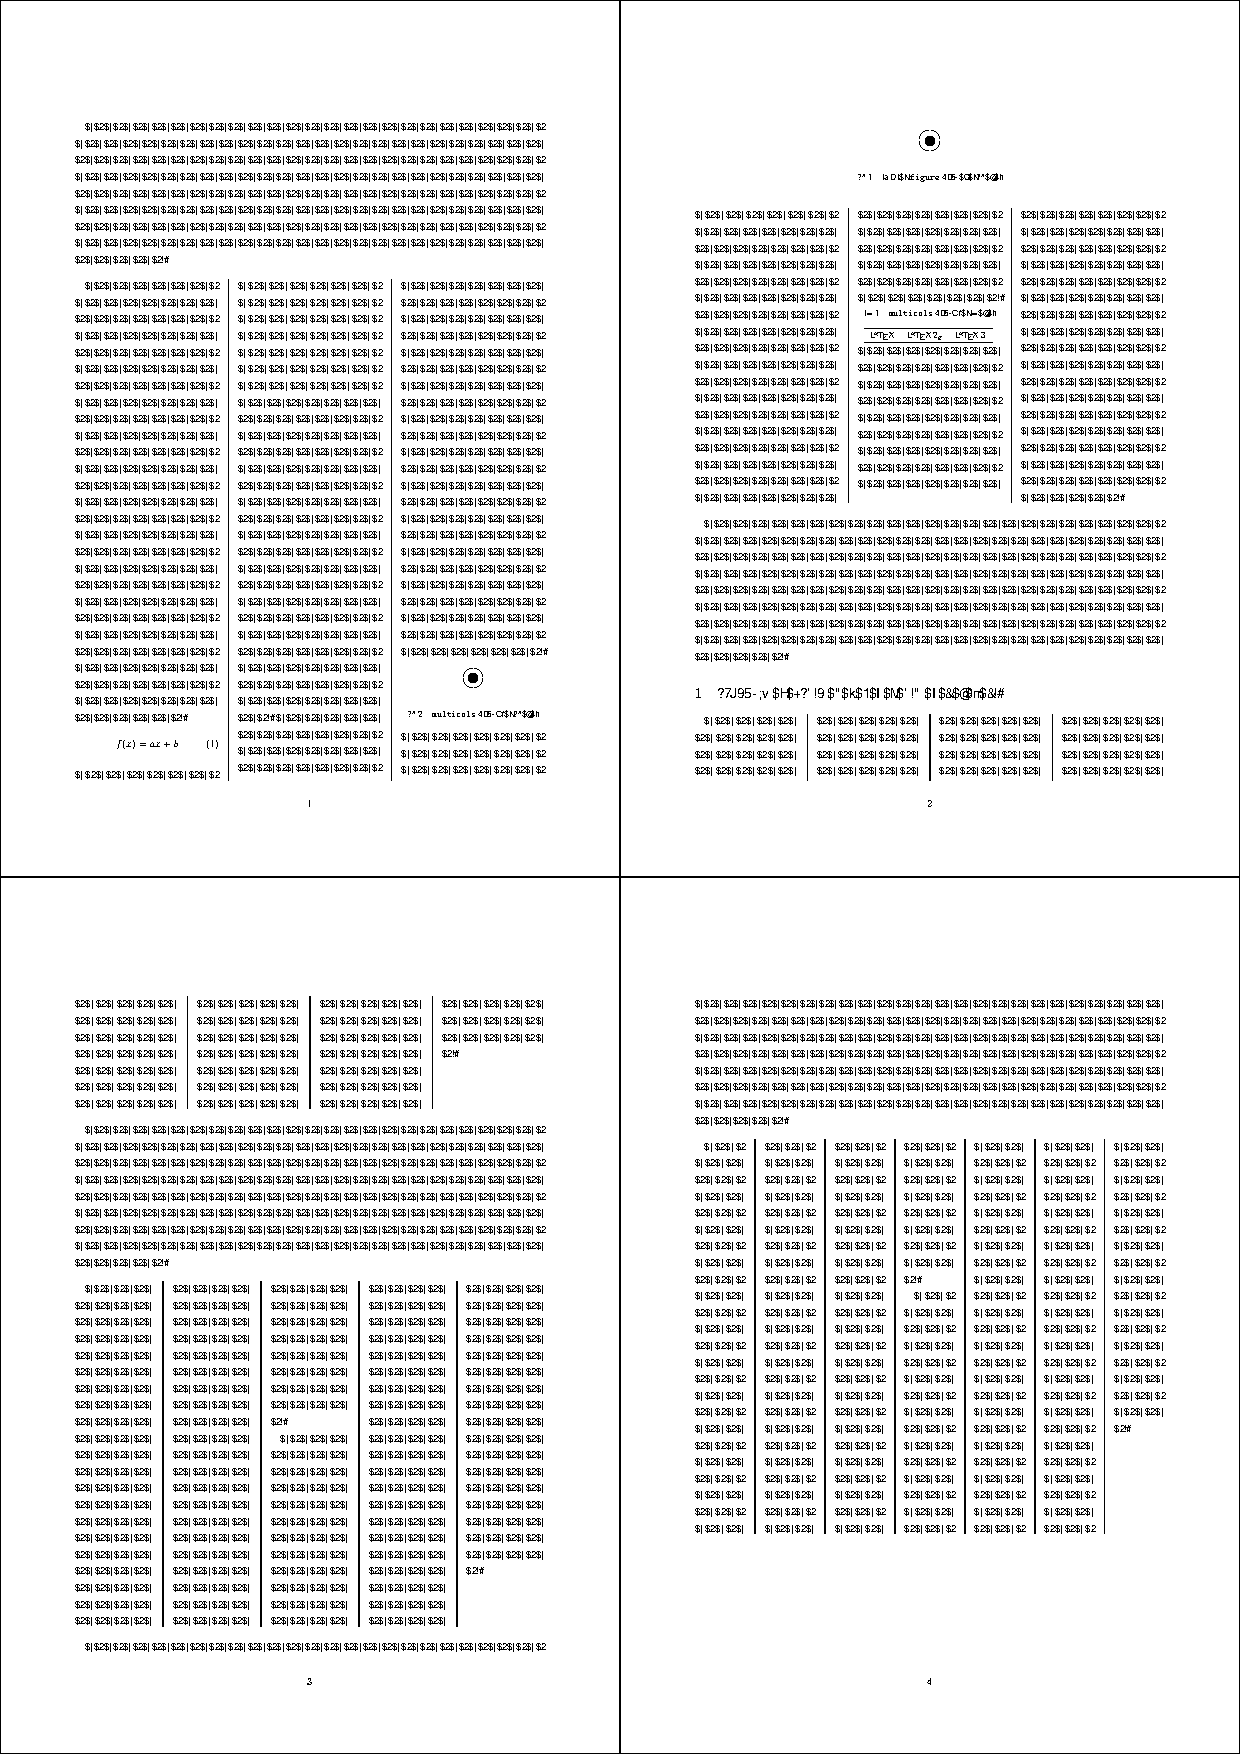
\includegraphics[width=\textwidth]{images/multicol.pdf}}
   \IOlabel
   \caption{\Y{multicol}の使用例の出力結果}\figlab{multicol}%
\end{figure}

\Person{Frank}{Mittelbach}の \Y{multicol} では 段抜きで配置する \E{figure*}
環境と \E{table*} 環境は許されますが,段の中に組まれる \E{figure}/\E{table}
環境は使えません.そのため,図をフロートさせずに配置するために
\E{myfigure}/\E{mytable} 環境を新設しています.ただし,フロートしない
ため図表の直前/直後で余計な空白が挿入されるので,これを手動で調整する (具
体的には関係する文の少し後に \E{myfigure}/\E{mytable} を記述する) 事に
なります.

段間の空白,段間に引かれる罫線,段の上端/下端の空きは次のように設定しま
す. 

\C*{columnseprule}%
\C*{columnsep}%
\C*{multicolsep}%
\begin{InTeX}
\columnseprule=.4pt % 段間に引かれる罫線
\columnsep=2zw %  段間の空白
\multicolsep=1zw % 段の上端/下端の空き
\end{InTeX}


\section{長さ} 
{\laTEX}における\K{長さ}には伸縮するものと
しないもの2種類があります.伸縮するものを
{\KY{可変長の長さ}}と呼び,伸縮しないものを\indindz{長さ}{可変長の}
{\KY{固定長の長さ}}と呼びます.\indindz{長さ}{固定長の}
可変長の長さは{\KY{スキップ}}と呼ばれる事が多いようですが,
本書では可変長の長さと呼びます.
可変長の長さは{\KY{長さ}},
{\KY{縮み率}},{\KY{伸び率}}の三つの
属性を持っています.固定長の長さは決まった値しか
持ちません.可変長の長さは縮み率と伸び率に従って
バネのように伸縮します.長さの定義には \cmd{newlength}が使えます.
\begin{Syntax}
\Cmd{newlength}\pa{綴り}\\
\Cmd{setlength}\pa{綴り}\pa{長さ} \\
\Cmd{addtolength}\pa{綴り}\pa{長さ}
\end{Syntax}
\cmd{setlength}で長さを設定します.\cmd{addtolength}
では元の長さにさらに長さを足します.\cmd{newlength}
で定義された長さは可変長にも固定長にもなって良い
事になっています.まず \cmd{newlength}で新規に
長さを定義します.次に \cmd{setlength}で
値を決めます.
\begin{InOut}
\newlength{\newa}\the\newa\\
\setlength{\newa}{10mm}\the\newa\\
\setlength{\newa}{10mm plus 3mm
   minus 2mm}\the\newa\\
\addtolength{\newa}{3mm}\the\newa
\end{InOut}
可変長の長さに値を足しても縮み率と伸び率には
影響しないのが例の出力から分かるでしょう.

長さを設定するには次の命令も使えます.
\begin{Syntax}
\Cmd{settowidth}\pa{綴り}\pa{要素} \\
\Cmd{settoheigth}\pa{綴り}\pa{要素} \\
\Cmd{settodepth}\pa{綴り}\pa{要素} 
\end{Syntax}
長さに対して要素の幅を代入するには \cmd{settowidth}を
使います.高さに関しては \cmd{settoheight},
深さには \cmd{settodepth}を使います.このような命令の
使い道を少し紹介しておきます.
\begin{InOut}
%\newlength{\newa} 
\newcommand{\fakewidth}[1]{%
  \settowidth{\newa}{#1}%
  \framebox[\the\newa][c]{\strut}}
解は{$\int f(x)dx$}となる.\par
解は\fakewidth{$\int f(x)dx$}となる.
\end{InOut}



\section{箱の操作}
まずは{\LaTeX}で用意されている{\KY{箱}}について説明します.
これらは\Fl{ltboxes.dtx}で定義されています.{\LaTeX}における箱とい
うのは文章や段落,数式や図表などの要素を格納する領域のようなものです.
{\LaTeX}の箱には\K{高さ}と\K{幅}と\K{深さ}の3種類の長さを
持っています.さらに箱のどの点を基準にするかという\K{基準点}と
いう座標も持ち合わせています.

\subsection{枠のない箱}
{\LaTeX}ではなんとも簡単に複数の要素を
一つの箱に収める事ができます.
\begin{Syntax}
\Cmd{makebox}\opa{幅}\opa{位置}\pa{要素}
\end{Syntax}

\cmd{makebox}では箱の幅と箱の中の要素の\indindz{幅}{箱の}%
位置を指定できます.箱の幅よりも要素の幅が狭いときに
箱の左側に配置\qu{\str l},中央に配置する\qu{\str c},
右側に配置する\qu{\str r},最後に要素を均一に配置する
\qu{\str s}の四つを使う事ができます.
\begin{InOut}
\makebox[3zw][l]{未来}と
\makebox[3zw][c]{函館}と
\makebox[5zw][r]{北海道}と
\makebox[5zw][s]{G o o d !}です.
\end{InOut}
要素の幅分の箱を作りたければ \cmd{mbox}を使います.
\begin{Syntax}
\Cmd{mbox}\pa{要素}
\end{Syntax}
引数を省略すると要素分の幅を確保し \cmd{makebox}を
使うよりも効率が良いです.
\begin{InOut}
\hspace*{\fill} 単なる予想ですが,
この箱の中では恐らく\mbox{改行が
起こりません.} 
\end{InOut}

\subsection{枠のある箱}


複数の要素を一つの塊として扱うようにするのが
{\LaTeX}における箱の役割のようなものです.
箱には枠を付ける事もできます.
\begin{Syntax}
\Cmd{framebox}\opa{幅}\opa{位置}\pa{要素}
\end{Syntax}
 \cmd{framebox}も \cmd{makebox}とほぼ同じですが\zindind{罫線}{の太さ}%
罫線の太さ \Cmd{fboxrule}と罫線と要素の
間隔 \Cmd{fboxsep}の二つの長さを設定できます.
 \cmd{fboxrule}は罫線の太さを, \cmd{fboxsep}は\zindind{枠}{の太さ}%
枠と要素との距離を長さで指定します.\zindind{枠}{と文字の間隔}%
\begin{InOut}
\framebox[3zw][l]{未来}と
{\fboxrule=3pt\framebox[3zw][c]{函
館}}と\framebox[5zw][r]{北海道}と
\framebox[5zw][s]{G o o d !}です.
\end{InOut}
 \cmd{makebox}と同じように引数を省略すると要素分の
幅を確保する \cmd{fbox}が使えます.
\begin{Syntax}
\Cmd{fbox}\pa{要素}
\end{Syntax}
\begin{InOut}
これは{\fboxsep=0pt\fbox{ぴったり
です}}.こちらは{\fboxrule=.8pt
\fbox{若干太い}}.
\end{InOut}

\subsection{広範囲な箱}\indindz{箱}{広範囲な}%

指定した箱の大きさで段落を組む \Cmd{parbox}
命令もあります.標準では字下げがされません\indindz{字下げ}{箱の中での}%
ので必要があれば \cmd{parindent}に長さを代入
してください.
\begin{Syntax}
\Cmd{parbox}\opa{位置}\opa{高さ}\opa{要素の位置}\pa{幅}%
\pa{文字列}
\end{Syntax}
\cmd{parbox}で作成された箱の基準をどこにするのかを
\va{位置}で指定します.位置には上部\qu{\str t},
中央\qu{\str c},下部\qu{\str b}の三つが使えます.
標準では中央になります.
\begin{InOut}
\parbox{13zw}{段落が終わる命令\par
を使っても改行されますが\par
標準では字下げされません.}
\end{InOut}
\begin{InOut}
\parbox[c]{4zw}{箱が中央に.}\ldots
\parbox[t][3zw][c]{4zw}{文字が中央,
上が基準}\ldots 
\parbox[b][3zw][t]{4zw}{文字が下に,
下が基準}\ldots
\end{InOut}
\zindind{ページ}{のような箱}ページのような箱を組む\env{minipage}環境もあります.
\begin{Syntax}
\verb|\begin{minipage}|\opa{位置}\pa{幅}\\
ページ内容\\
\verb|\end{minipage}|
\end{Syntax}
\Env{minipage}環境では段落が組まれますし,
脚注の出力も可能です.%
\index{脚注!minipage環境での@\texttt{minipage}環境での\zdash}%
\begin{InOut}
この環境は~
\begin{minipage}[t]{7zw}
ページを組みあげるので脚注%
\footnote{脚注です.}
もページの中に出力されます.
\end{minipage} 
~となります.
\end{InOut}

\subsection{箱の保存と使用}\zindind{箱}{の保存}\zindind{箱}{の再利用}%%
ある要素を箱の中に保存し,それを再利用できれば
エネルギー消費を減らす事ができます.
\begin{Syntax}
\Cmd{newsavebox}\pa{綴り}
\end{Syntax}
箱を保存するためには保存する場所の確保を \cmd{newsavebox}で
行います.{\LaTeX}が使っ
ても良い箱は数が限られているのであらかじめ
いくつくらい使うのかを宣言してあげます.
宣言するときはバックスラッシュを先頭に付けます.
箱の中に要素を保存するときは \cmd{savebox}か \cmd{sbox}命令を使います.
\begin{Syntax}
\Cmd{savebox}\pa{綴り}\opa{幅}\opa{要素の位置}\pa{要素}\\
\Cmd{sbox}\pa{綴り}\pa{要素}
\end{Syntax}
箱の幅や要素の位置を指定するときは \cmd{savebox}
を使います.もちろん幅を指定しないと要素の位置は
指定できません.
上記の命令のほかにも\Env{lrbox}環境があります.
行に収まるくらいの要素を\env{lrbox}環境の中に
記述すると\va{綴り}の箱に代入します.
\begin{Syntax}
\verb|\begin{lrbox}|\pa{綴り}\\
\va{要素}\\
\verb|\end{lrbox}|
\end{Syntax}

これまでの命令では箱を用意してその中に要素を保\zindind{箱}{の用意}%
存するだけですので,保存した箱を \Cmd{usebox}命令で使います.
\begin{Syntax}
\Cmd{usebox}\pa{綴り}
\end{Syntax}
\cmd{usebox}命令を使うと\va{綴り}の箱に
保存されている要素を複数回再利用できます.
\begin{InOut}
\newsavebox{\hoge} 
\savebox{\hoge}{\LaTeXe から
  \LaTeX\,3 へ}
\usebox{\hoge}, \usebox{\hoge}.\\
\usebox{\hoge}, \usebox{\hoge}.\\
\sbox{\hoge}{}  \usebox{\hoge}
\end{InOut}
{\LaTeX}の作業領域は限られていますので \Cmd{setbox}命令で\va{綴り}の箱を
使い終わったら空にします.


\subsection{箱の上げ下げ}\zindind{箱}{の上げ下げ}%
ある要素を箱の中に入れて,さらに上げ下げを
同時に行う \Cmd{raisebox}命令もあります.
\begin{Syntax}
\Cmd{raisebox}\pa{上げ下げ}\opa{高さ}\opa{深さ}\pa{要
 素}
\end{Syntax}
\cmd{raisebox}命令の中には文字列や他の箱も
挿入できます.
\begin{InOut}
それで,\raisebox{1zw}{あれ}は
\raisebox{-1zw}{これ}で,
\raisebox{1.5zw}{\fbox{枠付きの箱}}だ.
\end{InOut}


\subsection{罫線と下線}

箱とは違うのですが\KY{罫線}をここで紹介しておきます.
\begin{Syntax}
\Cmd{rule}\opa{上げ率}\pa{幅}\pa{高さ}
\end{Syntax}
 \cmd{rule}命令は使いものになります.見えない罫線を
引く事もできます.例えば幅が0\,ptでも高さのある
罫線,高さが0\,ptでも幅のある罫線が使えますから,
こんな使い方もできるわけです.枠の見える
状態での例を見てください.
\begin{InOut}
\newcommand*\RULE[2]{%
  \rule{0pt}{#1}\rule{#2}{0pt}}
未来 \fbox{\RULE{3zw}{4zw}}
函館 \fbox{\RULE{3zw}{2zw}}
\end{InOut}

箱とは違うのですが\KY{下線}も紹介しておきます.
下線は \cmd{underline}を使います.
\begin{Syntax}
\Cmd{underline}\pa{要素}
\end{Syntax}
 \cmd{underline}の中に箱を入れる事もできますし,
何を入れても構いません.
\begin{InOut}
\underline{\fbox{枠付きの箱}の下線}
はこのようにしますし,もちろん
\underline{下線}も表示できます.
\end{InOut}

\subsection{枠付きの箱その2\zdash\Y{fancybox}}\indindz{箱}{枠付きの}%
{\LaTeX}の標準では \Cmd{fbox}と \Cmd{framebox}命令が使えます.
\indindz{枠}{2重の}%
\begin{InOut}
\fbox{これは枠付きの箱} \\
\framebox[10zw][c]{日本太郎}\\
\fbox{\fbox{2重枠の箱}} \\
{\fboxrule=1pt\fbox{枠の太い箱}}\\
{\fboxsep=0pt\fbox{文字と枠がぴったり
な箱}}
\end{InOut}

\Person{Timothy}{Zandt}による\Sty{fancybox}を使ってみると
枠付きの箱を出しやすいでしょう.枠付きの箱に文字列を入れる
ための命令として \Cmd{shadowbox},\Cmd{doublebox},
\Cmd{ovalbox},\Cmd{Ovalbox}の四つがあります.
\begin{InOut}
\shadowbox{影付きの箱} \\
\doublebox{2重の枠 \\
\ovalbox{辺が丸い箱} \\
\Ovalbox{太くて辺が丸い箱}}
\end{InOut}

\sty{fancybox}を使うと\Env{Sbox}環境というものが使えて,
これは環境内のものを箱\pp{レジスタ}である \Cmd{TheSbox}に
保存します.このようにして保存した箱を \Cmd{fbox}などで
囲みます.例えば\env{minipage}を枠で囲む\env{fminipage}
環境を作成するのであれば次のようにします.

\begin{InTeX}
\newenvironment{fminipage}%
  {\begin{Sbox}\begin{minipage}}%
  {\end{minipage}\end{Sbox}\fbox{\TheSbox}}
\end{InTeX}


\begin{InOut}
\newenvironment{fminipage}%
  {\begin{Sbox}\begin{minipage}}%
  {\end{minipage}\end{Sbox}%
   \fbox{\TheSbox}}
\begin{fminipage}{.8\linewidth}
この環境は枠で囲まれます.というか,
囲んでくれないと困ります.
\end{fminipage}
\end{InOut}

数式環境などを枠で囲もうと思うとき,数式番号も
含めて枠の中に入れるのはちょっと面倒かもしれません.
\cmd{fbox}などの命令を使うとそこから数式を組み立てる
モードではなく文章を組み立てるモードになりますので,
もう1度数式環境を書きます.
\begin{InOut}
\( y = f(x) + \fbox{\(C\)}\) 
\begin{equation}
 \fbox{\(y = f(x)\)}
\end{equation}
\end{InOut}

番号付きの数式を文章幅いっぱいに枠で囲むには
\begin{quote}
 (\cmd{linewidth} \pp{文章幅} $-2$\cmd{fboxrule} $-2$\cmd{fboxsep})
\end{quote}
を計算します.これには\Sty{calc}パッケージが使えます.
\begin{InOut}
\usepackage{calc,fancybox} 
\fbox{\parbox{(\linewidth-
   2\fboxrule-2\fboxsep)}{
\begin{equation} y=f(x) 
\end{equation}}}
\end{InOut}

\env{eqnarray}環境は枠で囲もうと思うと\sty{fancybox}の
場合は\Env{Beqnarray}が用意されていますので,こちらの
環境を \cmd{fbox}などで囲みます.
\begin{InOut}
\fbox{\begin{Beqnarray}
 y & = & f(x)\\
   & = & 1/x
\end{Beqnarray}} 
\end{InOut}

\env{table}環境や\env{figure}環境などで見出しも
含まれる要素は \Cmd{Sbox} で一度保存したものを枠で
囲むようにします.こうすると
\begin{InTeX}
\usepackage{calc,fancybox}% プリアンブルで
\newenvironment{ftable}[1][htbp]%
  {\begin{table}[#1]
   \begin{Sbox}\begin{minipage}{%
  (\linewidth-2\fboxrule-2\fboxsep)}}%
  {\end{minipage}\end{Sbox}\fbox{\TheSbox}\end{table}} 
\end{InTeX}
のように\env{ftable}や\env{ffigure}のような環境が
定義できます.この出力例が\tabref{fancy}となります.
\begin{ftable}
\begin{center}
  \caption{\protect\LaTeX の歴史}\tablab{fancy}
  \begin{tabular}{ccc}
 \LaTeX\,2.09& \LaTeXe& \LaTeX\,3\\
 \end{tabular} 
\end{center}
\end{ftable}

\sty{fancybox}では\env{center}環境のように行揃えを
行う環境があります.これを枠で囲むには%
\zindind{左揃え}{を枠で囲む}%
\zindind{右揃え}{を枠で囲む}%
\zindind{中央揃え}{を枠で囲む}%
\Env{Bcenter},\Env{Bflushleft},\Env{Bflushright}
環境を使います.
\begin{InOut}
\fbox{\begin{Bcenter}
ここは \\ 中央揃えで \\ 
  枠付きです.
\end{Bcenter}}
\end{InOut}
\begin{InOut}
\fbox{\begin{Bflushleft}
ここは \\ 左揃えで \\ 
  枠付きです.
\end{Bflushleft}}
\end{InOut}
\begin{InOut}
\fbox{\begin{Bflushright}
ここは \\ 右揃えで \\ 
 枠付きになります.
\end{Bflushright}}   
\end{InOut}
\env{minipage}環境の中で行揃えの命令を使う事も
考えられますが,その場合は横幅を指定しないといけ
ないので,これらの環境は便利でしょう.
箇条書き環境も同様に\env{minipage}の中に入れて \cmd{fbox}で
囲む事も考えられますが,\sty{fancybox}では
\Env{Bitemize},\Env{Benumerate},\Env{Bdescription}の
三つがすでに定義されているので,これらの環境を
枠で囲みます.
\begin{InOut}
\fbox{\begin{Benumerate}
 \item 北海花子.
 \item 太郎君と花子さん.
 \item 日本太郎.
\end{Benumerate}}
\end{InOut}

\begin{comment}
 変換のときに
 ** WARNING ** Object reference with key "enumi.x.xx" is in use.
 ** WARNING ** Could not add Dests name tree entry...
 が出てくるかが,気にしないでね.
\end{comment}

\Cmd{verb}命令を枠で囲むときは \Cmd{VerbBox}命令を
使います.
\begin{InOut}
\VerbBox{\fbox}{
\verb|\VerbBox{\fbox}{\verb+\+}|}
\end{InOut}

\Env{verbatim}環境を枠で囲む場合はやはり先に
\env{Sbox}環境で囲んで \cmd{TheSbox}を枠で
囲むようにします.この場合\Env{fverbatim}環境を
定義したほうが便利でしょう.ただし,
この場合 \Cmd{VerbatimEnvironment}命令と\Env{Verbatim}環境を
併せて使わないとエラーになります.
\begin{InOut}
\newenvironment{fverbatim}[1]%
 {\VerbatimEnvironment 
 \begin{Sbox} \begin{minipage}{#1}%
 \begin{Verbatim}}{\end{Verbatim}%
  \end{minipage}\end{Sbox}%
  \fbox{\TheSbox}}
\begin{fverbatim}{.8\linewidth}
このべた書き環境は枠で囲まれて
出力されます.
\end{fverbatim}
\end{InOut}


枠付の箱を出力するために \LaTeX 標準の \E{framebox}環境
や \C{fbox} などが使用できますが,
もうすこし,角がまるかったり,数式などにも使えると便利です.
ある程度は好き好きシリーズの初級編で取り扱っているので,そちらを参照して
下さい.ここでは\Person{Timothy}{Zandt}による \Y{fancybox} をもう少し
細かく見てみましょう.
\begin{Syntax}
\C{boxput*}\xy{x}{y}\pa{下になる要素}\pa{上になる要素}
\end{Syntax}
という \C{boxput} 命令が使えます.使用例を参考にしてみて下さい.
\C{boxput} に星を付けると重ね合わせる順番が逆になります.
\begin{InOut}
\usepackage{fancybox,color}
\boxput(0,0){\color{blue}\Huge Draft}
{\color{red}\parbox{\linewidth}{%
こちらはなんでもかんでも\LaTeX 
でがんばります.\LaTeX は最高で
す.とにかく一度使ってみて下さい.}}
\end{InOut}
他にもページごと枠で囲む \C{fancyput} や \C{thisfancyput} なども
あります.
\begin{Syntax}
\C{fancyput*}\xy{x}{y}\pa{文章要素} \\
\C{thisfancyput*}\xy{x}{y}\pa{文章要素} 
\end{Syntax}
ここでは触れませんが \E{verbatim} 環境系の拡張がされています.


このほかにも\sty{fancybox}にはファイルから
読み込んだ行をべた書き環境に出力する命令なども
用意されています.





\section{空白の挿入}
{\LaTeX}にはいろいろ空白が用意されているのですが,
それらは{\KY{空き}}に含まれます.単語間に挿入される
程度の空きを基準とするとその4倍の空きを
\qu{quad}\pp{クワタ}と呼びます.和文組版では
空きの基準となるのは全角1文字分の幅であり,これを
\emph{全角空白}などと呼びます.全角空白一つ分の
空きを\emph{全角空き},全角空白二つ分の空きを
\emph{倍角空き}と呼びます.さらに4分の1の場合は
\emph{四分空き},6分の5ならば\emph{二分三分}と
呼んだりします.欧文の\qu{quad}と和文の\yo{クワタ}
では若干長さが異なりますので,本書では二つを
区別して表します.

\subsection{水平方向の空き}
\indindz{空き}{水平方向の}
\zindind{改行}{を許す空き}%
水平方向の空きにはその両側での改行を許すものと
許さないものがあります.主な空きを制御する
命令は\tabref{yokokuhaku:break}の通りです.
\tabref{yokokuhaku:break}は基本的に
空きの前後での改行を行っても良い事になっています.
\begin{table}[htbp]
\begin{center}
\caption{改行を許す水平方向の空き}\tablab{yokokuhaku:break}
\glossary{" @\hspace*{-1.2ex}\verb*+"\" +}%"
\indindz{空白}{単語間}%
\begin{tabular}{ll}
\TR
\Th{命令}         & \Th{意味}  \\
\MR
\verb*|\ |   & 適切な\emph{単語間空白} \pp{約1/4\,quad分}  \\
\C{quad}   & 1\,quad分の空き \\
\C{qquad}  & 2\,quad分の空き \\
\C{enspace}& 1/2\,quad分の空き\\
\C{enskip} & 適切な約1/2\,quad分の空き\\
\C{thinspace}    & 1/5\,quad分の空き\\
\C{negthinspace} & $-$1/5\,quad分の空き\\
\BR
\end{tabular}
\end{center}
\end{table}

%\tabref{yokokuhaku:break}は基本的に
%空きの前後での改行を行っても良い事になっています.

\begin{InOut}
ユーザが{\quad}原稿の中{\qquad}で空き
の調節を直接\ するのは好ましくない.
\end{InOut}

\tabref{yokokuhaku:break}の命令は改行を
許しますが\tabref{yokokuhaku:nobreak}では
空きの前後での改行を許しません.
\zindind{改行}{を許さない空き}%
改行を許さないので行頭・行末が不揃いに\index{行末}
なるときがあります.


\begin{table}[htbp]
\begin{center}
\caption{改行を許さない水平方向の空き}\tablab{yokokuhaku:nobreak}
\glossary{" @\hspace*{-1.2ex}\verb+"\"!+}%
\index{"~@\verb+"~+}%"
\glossary{"~@\verb+"~+}%"
\begin{tabular}{ll}
\TR
\Th{命令}     & \Th{意味}  \\
\MR
\Cmd{,}  & 3/18\,quad分の空き\\
\Cmd{:}  & 4/18\,quad分の空き\\
\Cmd{;}  & 5/18\,quad分の空き\\
\verb|\!|& $-3/18$\,quad分の空き\\
\verb|~| & 適切な\emph{単語間空白} \\
%\Cmd{hspace*}\pa{長さ}& 
\BR
\end{tabular}
\end{center}
\end{table}

%改行を許さないので行頭・行末が不揃いに\index{行末}
%なるときがあります.

\begin{InOut}
Donald~E. Knuth made \TeX\@. 
Leslie~Lamport made \LaTeX\@.
\end{InOut}

自分で水平方向の空きの長さを指定するならば \Cmd{hspace*}
命令が使えます.
\begin{Syntax}
\Cmd{hspace*}\opa{長さ}
\end{Syntax}
アスタリスクを付けると行頭・行末でも使えるようになります.
\begin{InOut}
日本太郎\hspace{2zw}ならば\par
\hspace*{-2zw}である.
\end{InOut}
\hito{奥村}{晴彦}の\Cls{jsclasses}を使っているときに
は\qu{\str{pt}}や\qu{\str{cm}}などの単位は使わずに
\qu{\str{truept}}や\qu{\str{truecm}}などを使わないと
長さがずれます.これが面倒ならば文章で使用されている
フォントに応じて基準の変わる\qu{\str{em}}や\qu{\str{zw}}
などを使ってください.

\subsection{垂直方向の空き}
\indindz{空き}{垂直方向の}

自分で長さを指定する垂直方向の空きにおいて
は \cmd{addvspace}と \cmd{vspace*} の二つが使えます.
\cmd{vspace*} はアスタリスクを付けないとページの最上部・最下部
では有効になりません.あらかじめ長さの決まっている
垂直方向の空きとして \cmd{smallskip},\cmd{midskip},
\cmd{bigskip}の三つがありますが,これは\emph{スキップ}
と呼ばれるもので可変長の空きが挿入されます.
%\yo{大体で良いからこれくらいの空きを入れてね.}程度の
%意味を持っています.
\yo{見映えが損なわれない程度におおよそ指定した長さの空きを挿入してほしい}と
いうような意味合いを持っています.
\begin{table}[htbp]
\begin{center}
\caption{垂直方向の空き}\tablab{tatekuhaku}
  \begin{tabular}{ll}
 \TR
 \Th{命令}            & \Th{意味} \\
 \MR
 \C{smallskip}& 3\,pt $\pm$1\,ptの空き \\
 \C{medskip}  & 6\,pt $\pm$2\,ptの空き \\
 \C{bigskip}  & 12\,pt \pp{$+$4\,ptか $-$2\,pt} の空き \\
 \BR
 \end{tabular}
\end{center}
\end{table}
垂直方向の空きは紙面の多くの部分を空きで占有するので
無駄が多くなります.{\LaTeX}では図表と段落のあいだや
そのほか必要と思われる所には半自動的に
空きが挿入されるようになっておりますので,闇雲に
垂直方向の空きを挿入するのは好ましくないと思われます.

長さを自分で指定して空きを挿入する場合
は \cmd{vspace*} と \cmd{addvspace}が使えます.
\begin{Syntax}
\Cmd{addvspace}\pa{長さ}\\
\Cmd{vspace*}\pa{長さ} 
\end{Syntax}
\cmd{vspace*} のアスタリスクを外すとページの最上部・最下部での
空きの挿入が有効になりません.\cmd{addvspace}は
直前の空きがどれくらいかも調べているので \cmd{vspace}
よりも適当な空きを挿入します.
\begin{InOut}
この\vspace*{2zw}だと全角2文字分の
垂直方向の空きが挿入されると思われます.
\end{InOut}


\section{伸縮する糊}
{\LaTeX}ではバネのように伸縮する\emph{糊}のような
便利な道具があります.これは活版印刷時代における
活字職人が経験で挿入する\KY{込め物}に似ています.

{\LaTeX}においてもある領域の中での空きを制御するためとか,適切な表示をす
るための込め物が使われます.{\LaTeX}で使われる込め物は{\KY{グルー}}と呼
ばれています.グルーは伸縮自在でバネのように要素と要素をくっ付けるので伸
縮する\emph{糊}とも呼ばれています.

グルーは特別な単位\qu{\str{fil}}と\index{fil@\texttt{fil}}%
\index{fill@\texttt{fill}}\qu{\str{fill}}によって定義されています.
\qu{\str{fil}}は良い\ruby{按}{あん}\ruby{排}{ばい}
で0からかなり大きい空きまで挿入する働きを
します.\qu{\str{fill}}は\qu{\str{fil}}よりも
大きく無限に近い空きを挿入する働きをします.
\begin{table}[htbp]
\begin{center}
\caption{{\protect\LaTeX}で使用できるグルー}
\tablab{gulue:fil}
  \begin{tabular}{ll}
 \TR
 \Th{命令}  & \Th{意味} \\
 \MR
 \Cmd{hfil}  & 水平方向にかなり大きく伸びる空き\\
 \Cmd{hfill} & 水平方向に無限に大きく伸びる空き\\
 \cmd{hss}   & 水平方向にかなり大きく伸び縮みする空き\\
 \MR
 \cmd{vfil}  & 垂直方向にかなり大きい空き\\
 \cmd{vfill} & 垂直方向に無限に大きい空き\\
 \cmd{vss}   & 垂直方向にかなり大きく伸び縮みする空き\\
 \BR
 \end{tabular}
\end{center}
\end{table}
\qu{\str{fil}}は\qu{\str{fill}}よりも弱いので
\qu{\str{fill}}のほうが優先されます.
\begin{InOut}
この空き{\hfil}は{\hfil}かき消されません.\par
この空きは{\hfil}恐らく{\hfill}かき消されます.
\end{InOut}
\qu{\str{fil}}と\qu{\str{fill}}の二つのグルーの
両方を使っている場合は空きが挿入されない場合があ
りますから気を付けてください.

もう少し相対的なグルーを挿入するには
\cmd{stretch}を使います.
\begin{Syntax}
\Cmd{stretch}\pa{整数}
\end{Syntax}
これは\qu{\str{fill}}の何倍かのグルーを挿入しても
良いようにするために使用できます.
\begin{InOut}
hoge\hspace{\stretch{3}}hoge%
\hspace{\stretch{1}}hoge.\par
hoge\hspace{\fill}hoge\hspace{\fill}
hoge.\par
\end{InOut}
\Cmd{fill}は \cmd{hspace}や \cmd{vspace}の引数に
使う事ができるグルーです.
例えばページの最上部に無限に近いグルーを
挿入するときは以下のようにします.
\begin{InOut}
\vspace*{\fill}を使ってもこの出力例で
は伸びません.
\end{InOut}

\subsection{空白ではないグルー}
\cmd{hfil}や \cmd{hfill}は空白を挿入するグルーでした.そうではなく,与え
られた領域を程よく文字列や要素で埋めてくれる込め物もあると便利です.目次
でも使われているのがお分かりになるでしょう.これらを{\KY{リーダ}}と呼び
ます.{\LaTeX}であらかじめ定義されているリーダは\tabref{leaders}となりま
す.

\qu{\str{fill}}ですから無限に伸びます.
\begin{table}[htbp]
\begin{center}
\caption{主なリーダ}\tablab{leaders}
\begin{tabular}{lp{10zw}}
\TR
\Th{命令} & \Th{出力例} \\
\MR
\Cmd{dotfill}	    & \dotfill\\
\Cmd{hrulefill}     & \hrulefill\\
\Cmd{leftarrowfill} & \leftarrowfill\\
\Cmd{rightarrowfill}& \rightarrowfill\\
\Cmd{downbracefill} & \downbracefill\\
\Cmd{upbracefill}   & \upbracefill\\
\BR
\end{tabular}
\end{center}
\end{table}
\cmd{dotfill}と \cmd{hrulefill}は\Fl{ltplain.dtx}で,
それ以外は\Fl{fontdef.dtx}にて定義されています.
段落中で使うと段の終わりまで伸びます.
\begin{InOut}
\makebox[5zw][l]{未\dotfill 来}\\
\hrulefill\\
北海\leftarrowfill 道と\\
北方領土\rightarrowfill\par
\end{InOut}
これらのリーダは \Cmd{leaders}という命令によって
定義されています.自分でこのような命令を定義した
いときは \Cmd{leaders},\Cmd{cleaders},\Cmd{xleaders}
の三つが使えます.
例えば領域を\yo{未来}で埋めるような命令ならば
次のようになります.
\begin{InOut}
\newcommand{\hogefill}{\leavevmode
\leaders\hbox{未来}\hfill\kern0pt}
\hogefill\par
そう\hogefill だよ.\par
\end{InOut}


\section{付録の追加}
\index{付録の追加}
文書の最後に付録としてプログラムリストを載せるとか,
本文とは直接的に関係のない資料を載せるときは \C{appendix}
命令を使うか,\Env{appendix}環境を
使うかの2通りの方法があります.\env{appendix}環境を
使う場合は付録の範囲を指定できます.
\begin{Syntax}
 \verb+\begin{appendix}+\\
   \va{追加する内容}\\
 \verb+\end{appendix}+
\end{Syntax}
%あえて \cmd{appendix}命令を使う必要もないでしょう.
この命令を付けた後の文章は付録として扱われ,見出し
の番号付けが自動的に大文字のアルファベットに変更さ
れ,\qu{A}からカウントされるようになります.あとは
通常通り見出しの定義をして文章を記述するだけです.



\section{原稿を複数のファイルに分ける}\zindind{原稿}{の分割}%
大規模な文書になるとそれを一つのファイルにまとめるのは効
率が悪い場合があります.第3章は田中さんが編集し,第5章は斉
藤さんにお任せする,という状況では第3章と第5章の原稿は別
々に存在させたいものです.この場合は原稿を複数のファイル
に分けます.
\begin{Syntax}
\Cmd{include}\pa{ファイル名,\ldots}\\
\Cmd{input}\pa{ファイル名,\ldots} \\
\Cmd{includeonly}\pa{ファイル名,\ldots}
\end{Syntax}
\cmd{include}命令はファイルを読み込むときに必ず新しいペ
ージから始めます.大規模な文書の章の区切りや節の区切りなど
で使用します.この命令で取り込むときはファイルを章ごとに
\pp{\cmd{chapter}ごと}に分ける事が考えられます.
\cmd{input}はそのままの意味で指定されたファイルを
そのまま親の{\LaTeX}のソースファイルに取り込みます.
取り込むファイルの拡張子が\exten{tex}ならば拡張子
を省略しても構いません.

例えば論文を作成する場合は次のように分割する事もできます.

\begin{InText}
%#!platex
\documentclass[dvipdfmx,papersize]{jsbook}% クラスファイル
\usepackage{amsmath,amssymb,bm,verbatim,listings}% 必要なマクロ
\includeonly{2joron}% ある章だけを読み込む
\begin{document}
\maketitle
\tableofcontents
\listoffigures
\listoftables
\frontmatter%       前付
\include{0preface}% 前書き
\include{1thanx}%   謝辞
\mainmatter%        本文
%\doublespacing %     
\include{2joron}%   序論
\include{3honron}%  本論
\include{4keturon}% 結論
%\singlespacing %     
\begin{appendix}%   付録
\include{5code}%    付録: ソースコード
\end{appendix}%
\backmatter%        後付
\bibliographystyle{jplain}% 文献形式
\bibliography{ron}% 参考文献
\end{document}
\end{InText}

%\begin{comment}
%\begin{InTeX}
%%#!platex
%\documentclass[dvipdfmx]{funthesis}[2004/11/10]
%\usepackage{gsset}%    設定ファイル
%%\includeonly{05con}
%\makeatletter
%%\def\Gin@extensions{.jpg,.jpeg,.png,.bmp,.pdf.Z}
%\makeatother
%\begin{document}
%\maketitle%          目次
%\input{00abst}%      概要
%\frontmatter %        前付け
%\tableofcontents %   目次
%\listoffigures %     図目次
%\listoftables %      表目次
%\mainmatter %         本文
%%%\doublespacing %      
%\include{01preface}%  序論
%\include{02prevwork}% 関連研究
%\include{03plan}%     提案する理論
%\include{04exp}%      実験と評価
%\include{05con}%      考察
%\include{06postface}% 結論と今後の展開(新規性のある考察のみ)
%%%\singlespacing
%\include{07thanx}%    謝辞
%\include{08ref}%      参考文献
%\appendix %           以降,付録(付属資料)であることを示す
%\include{10report}%   システム仕様
%\end{document}
%\end{InTeX}
%\end{comment}




%\section{付録の追加}\index{付録の追加}
%文書の最後に付録としてプログラムリストを載せるとか,
%本文とは直接的に関係のない資料を載せるときは \Cmd{appendix}
%命令を使うか,\Env{appendix}環境を使うかの2通りの方法があります.
%\env{appendix}環境を
%使う場合は
%\begin{quote}
% \verb+\begin{appendix}+\\
% \va{追加する内容}\\
% \verb+\end{appendix}+
%\end{quote}
%という記述が可能ですから付録の範囲を指定できます.
%あえて \cmd{appendix}命令を使う必要もないでしょう.
%この命令を付けた後の文章は付録として扱われ,見出し
%の番号付けが自動的に大文字のアルファベットに変更さ
%れ,\qu{A}からカウントされるようになります.あとは
%通常通り見出しの定義をして文章を記述するだけです.

% 何か別の案を考える \w \W
%\section{人名の敬称の統一}
%一般的に一つの文書において人名の敬称は統一します.
%これはけっこう面倒な作業で,登場する人名を索引に
%追加する場合などの手間もあるかも知れません.その
%場合,新たに何か便利な命令を作るのが良いでしょう.
%始めに索引に追加しない簡単な例を示します.この場合,
%敬称だけを付け足す簡単なマクロです.
%
%\begin{InTeX}
%\newcommand{\hito}[1]{#1氏}
%\end{InTeX}
%
%これだけです.後は
%
%\begin{InTeX}
%\hito{渡辺徹}のおかげで1輪車に乗れるようになった.
%\end{InTeX}
%
%のように使うだけです.


%索引にも追加する場合を
%考えましょう.読みについては辞書ファイルに登
%録すると仮定して
%\begin{InText}
%\newcommand{\hito}[1]{\index{#1}#1氏}
%\end{InText}
%とするか
%\begin{InText}
%\newcommand{\hito}[1]{%
%   \index{#1}%
%   \index{人名!#1}%
%   #1氏}
%\end{InText}
%が考えられるでしょう.さらに並び替え用の
%文字と表示用の語を別にしたいならば
%\begin{InText}
%\newcommand{\Hito}{\@ifnextchar[{\yomi@Hito}{\@Hito}}
%\newcommand{\yomi@Hito}[2][]{\index{人名!#1@#2}%
%   \index{#1@#2}#2氏}
%\newcommand{\@Hito}[1]{\index{人名!#1}%
%   \index{#1}#1氏}
%\end{InText}
%と定義しておき,
%\begin{InText}
%\Hito{Frank Mittelbach}と
%\Hito[Rainer Schopf]{Rainer Sch\"opf}の共同制作.
%\end{InText}
%として使えます.これで全て大丈夫というわけでは
%ありませんが人名ならば問題ないと思われます.


\section{翻訳作業}
\seclab{honyaku}
しばしば日本語ではない言語で書かれた文書を訳す作業
があります.運良く原書の{\LaTeX}の原稿が手に入った
とすると,作業は幾分楽になります.例えば以下のよ
うな原稿があったとします.

\begin{InTeX}
Hello, everyone! I'm a student at Future University Hakodate. 
Today, please let me talk about my future plan. 
First, ...
\end{InTeX}

これを工夫せずに普通に翻訳すると次のようになるでしょう.

\begin{InTeX}
皆さん,こんにちは.私は公立はこだて未来大学の生徒です.
今日は私の未来計画についてお話したいと思います.まず,
\end{InTeX}

どうせなら原書の英文も削除したくありません.

\begin{InTeX}
%Hello, everyone! I'm a student at Future University Hakodate. 
皆さん,こんにちは.私は公立はこだて未来大学の生徒です.
%Today, please let me talk about my future plan. 
今日は私の未来計画についてお話したいと思います.
%First, ...
まず,
\end{InTeX}

このように入力すると英文と和文の対応が取れて分かりやすいでしょう.
ワープロソフトではマネのできない芸当です.1行ずつに分ける必要はなく,非
常に長い文章の場合は1段落ごとに対応させるのも良いでしょう.


\section{用語の統一}\seclab{xspace}
%\secref{honyaku}のような場合には
%用語の統一というが必要になってきます.
%一つの書籍を複数の訳者で共同翻訳するときに
%専門用語の場合や新語の場合は語句を統一しな
%ければ,読者を混乱させます.統一されてい
%ない事態を避けるためにはマクロを作成して
%おきます.
%\begin{InTeX}
%Hello, everyone! I'm a student at Future University-Hakodate. 
%\end{InTeX}
%という文章があったとして
%`Future University-Hakodate'とい
%う用語が新語であったとしましょう.
%この用語をどんな単語に訳すのかを
%まだ決められない段階では次のよう
%なマクロを作成します.
%\begin{InTeX}
%\newcommand{\FUN}{Future University-Hakodate}
%\end{InTeX}
%訳者のあいだで用語の訳が決まったならば
%\begin{InTeX}
%\newcommand{\FUN}{公立はこだて未来大学}
%\end{InTeX}
%とします.他にも人名や専門用語,
%難解な単語などに遭遇したときはこ
%のようなマクロを全ての訳者が参照
%できるファイルに収めておきます.
\zindind{用語}{の統一}
大規模な文書の場合は,\K{用語の統一}というのが必要にな
ってきます.一つの文書を複数の訳者で共同翻訳するときに専
門用語の場合や新語の場合は語句を統一しなければ,読者を混
乱させます.統一されていない事態を避けるためにはマクロを
作成しておきます.

\begin{InText}
Hello, everyone! I'm a student at Future University-Hakodate. 
\end{InText}

という文章があったとして`Future University-Hakodate'とい
う用語が新語であったとしましょう.この用語をどんな単語に
訳すのかをまだ決められない段階では次のようなマクロを
作成します.

\begin{InText}
\newcommand*{\FUN}{Future University-Hakodate}
\end{InText}

訳者のあいだで用語の訳が決まったならば次のようにします.

\begin{InText}
\newcommand*{\FUN}{公立はこだて未来大学}
\end{InText}

他にも人名や専門用語などで,非常に長い文字列を
文書の中で何度も記述しなければならないときは,
上記のように \C{newcommand*} 命令で文字列を定義する事になります.

ただし,欧文の場合は\Y{xspace}を使わなければ,適切な
空白が挿入されない場合がありますので,次のように定義します.
\indindz{空白}{コマンドの後の}
\begin{Syntax}
\C{newcommand*}\pa{コマンド名}\texttt\lb\va{文字列}\C{xspace}\texttt\rb
\end{Syntax}

\begin{InOut}
\usepackage{xspace} 
\newcommand*\LC{Logical OR}% (×)
\LC is good?  `\LC' is also ok.
\renewcommand*\LC{Logical OR\xspace}
\LC is funky! `\LC' is also ok.
\end{InOut}


%\section{本書の構成法}
%
%本書を執筆するにあたってのクラスファイル,マクロパッケージ,原稿
%などは\K{全て}著者のウェブページ\footnote \webThorTypo にて公開して
%います.さらに本書の印刷用の PDF,hyperref などによって便利な操作が
%可能な閲覧用 PDF も公開しております.パソコンなどに閲覧用 PDF を保存
%しておけば文字列検索もできますし,紙媒体の本書がない時にも活用できる
%ものと思います\footnote{この時代にある情報を紙媒体だけでしか入手する
%術がないというのは,少々伝統的過ぎると感じております.}
%
%% 原稿のコメントには著者の悲痛な叫び,durty joke が含まれます.
%本書の出力と「同じような出力を \LaTeX で実現したい」と感じたので
%あれば,直接原稿ファイルを参照してみてください.

%\begin{description}
%\item[クラス]
% \Hito{奥村}{晴彦}による \Cls{jsbook} を基本的なクラスファイルとして,
% よい加減に変更を加えています.
%
%\item[書体]
% % 何分,判型が A5 で,しかもページ数が 400 程度と,資源が少ないとです
% 和文には平仮名を詰め組みとした ヒラギノ基本 5 書体を使っています.
% 欧文は次のような設定になっています.
%\begin{InTeX}
%\usepackage{amsmath,amssymb}
%\usepackage[T1]{fontenc}
%\usepackage{textcomp}
%\usepackage{type1ec}
%\end{InTeX}
%
%\item[マクロ]
% 自作のマクロパッケージ \Fl{joumac.sty} を使っています.\fl{joumac.sty}
% の説明書は \Fl{joumac.dtx}というファイルで存在します.これを通常の
% \pLaTeX でタイプセットすると \Prog{DocStrip}というユーティリティに
% よって文書が整形されます.
%
%%\item[]
%\end{description}



\section{色の指定\zdash\Y{color}}\index{色}
{\laTEX}では白と黒の2色しか理解できません.
他の色を表現しようと思えば\Sty{color}パッケージなど
の力を借りて\Z{デバイス}ドライバに全てを任せる
事になります.ですから色はドライバに依存しますし,プリンタが
モノクロプリンタならばどうがんばってもグレースケール
のページしか出力できません.

色には{\KY{色相}}・{\KY{明度}}・{\KY{彩度}}
の三つの要素があります.色相とは青や緑などの波長の種類,
明度はその波長の明るさ,彩度は黒色の少なさを表します.
%色相については\kutiref{sikiso}を,明度と彩度
%の相関については\kutiref{meisai}を参照してください.


\subsection{要素に色を付ける}
{\LaTeX}は白と黒の2色しか理解できません.ですから
そのほかの色を付ける場合はデバイスドライバに
全てを任せます.グレースケールでも同様です.
色を付けるためには\sty{graphics}パッケージと同封
されている\Person{David}{Carlisle}が作成した
\Sty{color}パッケージを使います.\sty{color}を
使うにはまず\sty{graphicx}と同じように使用する
デバイスドライバを指定します.\prog{\Dvipdfmx}
などを使っているときは次のようにします.

\begin{InTeX}
\usepackage[dvipdfmx]{color} 
\end{InTeX}

パッケージオプションとして
次のようなものがあります.
\begin{description}
 \item[\Option{usenames}] \sty{color}パッケージで
  定義されている色の名前を全て使えるようにします.
%\option{usenames}で使用できる色名は\kutiref{color}
%の通りです.
 \item[\Option{dvipsnames}] \prog{dvips}で
使用できる色を名前を指定して使えるようにする.
\end{description}

\begin{Prob}
以下のファイル\fl{colortest.tex}をタイプセットし,さらに \Dvipdfmx によ
り PDF に変換し,その出力結果を吟味してください.

\begin{InTeX}
%#!F=hoge; platex $F.tex && dvipdfmx $F && open $F.pdf
\documentclass[10pt,dvipdfmx,papersize]{jsarticle}
\usepackage{type1ec,multicol}
\usepackage{color}
\pagestyle{empty}
\begin{document}
\renewcommand \DefineNamedColor[4]{%
   \textcolor[#3]{#4}{\rule{2em}{1em}}\space{#2}\\}
\parindent=0pt 
\begin{multicols}{3}
   \input{dvipsnam.def}
\end{multicols}
\end{document}
\end{InTeX}

実際にご自分が持っている(カラー/モノクロ)のプリンタで
上記のファイルを印刷してください.さらに印刷したものと
ディスプレイでプレビューしているファイル\fl{colortest.pdf}
を見比べてください.カラーで出力した方は一度モノクロでも
印刷してみてください.

もしも,差があるようであれば,どのような差があるのか頭の
中で整理してください.
\end{Prob}

%の二つも指定するのが良いと思われますので
%\begin{InTeX}
%\usepackage[dvipdfm,usenames]{color} 
%\end{InTeX}
%のようにします.
色の指定には四つあります.
\begin{description}
 \item[\str{rgb}] Red,Green,Blueの3色を
 混ぜ合わせて\emph{加法混色}で色を指定します.
 それぞれの色は0から1のあいだで指定します.
 \item[\str{cmyk}] Cyan,Magenta,Yellow,Blackの4色を
 混ぜ合わせて\emph{減法混色}で色を指定します.これも0から1のあいだで
 指定します.
 \item[\str{gray}] グレースケールで0から1のあいだで濃さを決めます.
 \item[\str{named}] あらかじめ定義された名前を使う事を
 意味します.
\end{description}

新規に色の名前を定義するときは \cmd{definecolor}を
使います.
\begin{Syntax}
\Cmd{definecolor}\pa{名前}\pa{種類}\pa{値}
\end{Syntax}
\va{種類}には上記の四つが選択できます.
例えば以下のように定義します.

\begin{InTeX}
\definecolor{MyGray}{gray}{0.85}
\definecolor{MyRed}{rgb}{0.3,0,0}
\definecolor{MyYellow}{cmyk}{}
\end{InTeX}

文字列の色は \cmd{textcolor}を使って色を指定します.\indindz{色}{文字の}
\begin{Syntax}
\Cmd{textcolor}\pa{色} \\
\Cmd{textcolor}\opa{種類}\pa{値}\pa{文字列}
\end{Syntax}
ある範囲中の要素には \cmd{color}命令で指定します.
\begin{Syntax}
\Cmd{color}\pa{色}  \\
\Cmd{color}\opa{種類}\pa{値}
\end{Syntax}
\begin{InOut}
\textcolor{Gray}{この文字は灰色}\\
\textcolor[rgb]{1,0,0}{赤らしく}\\
{\color{Gray}{\fbox{枠も文字も灰色
です.}}}
\end{InOut}

%基本色を \cmd{color}命令で指定せずにそのまま
%色の名前を使えるようにするには
%\begin{InTeX}
%\newcommand{\black}{\color{black}}
%\newcommand{\gray}{\color{Gray}}
%\newcommand{\white}{\color{white}}
%\newcommand{\red}{\color{red}}
%\newcommand{\green}{\color{green}}
%\newcommand{\blue}{\color{blue}}
%\newcommand{\cyan}{\color{cyan}}
%\newcommand{\magenta}{\color{magenta}}
%\newcommand{\yellow}{\color{yellow}}
%\end{InTeX}
%のように定義するだけです.
%\begin{InOut}
%\newcommand{\gray}{\color{Gray}}
%{\gray ここは灰色になります}
%\end{InOut}

ページの背景色を指定するときは \cmd{pagecolor}命令を使います.
\zindind{ページ}{の背景色}\indindz{色}{ページの}%
\begin{Syntax}
\Cmd{pagecolor}\pa{色}\\
\Cmd{pagecolor}\opa{種類}\pa{値}
\end{Syntax}
これは命令を使ったそのページからずっと色の
指定が有効ですので,1ページだけの色を変更したい
ときはページの切り替わるだろう部分で色を
元々の色に戻します.

\indindz{箱}{枠付きの}枠付きの箱の背景を指定できる \cmd{colorbox}命令があります.
\begin{Syntax}
\Cmd{colorbox}\pa{色}\pa{文字列}\\
\Cmd{colorbox}\opa{種類}\pa{値}\pa{文字列}
\end{Syntax}
\begin{InOut}
\colorbox{red}{背景が赤になる}\\
\colorbox[gray]{.8}{背景は灰色}\\
\colorbox{black}{\color{white}%
  背景が黒で文字は白}
\end{InOut}
\zindind{枠}{の色}%
さらに枠の色とその背景の色を指定できる \C{fcolorbox}
もあります.
\begin{Syntax}
\Cmd{fcolorbox}\pa{枠の色}\pa{背景色}\pa{文字列}\\
\Cmd{fcolorbox}\opa{種類}\pa{枠の色の値}%
  \pa{背景色の値}\pa{文字列}
\end{Syntax}
\C{fcolorbox}では \cmd{fbox}と同じように \C{fboxrule}
と \C{fboxsep}を調整できます.
\begin{InOut}
\fcolorbox{red}{blue}
  {枠が赤で背景が青}\\
\fcolorbox[gray]{.5}{.8}
  {枠も背景も灰色}\\
{\fboxrule=2.4pt\fcolorbox{blue}
  {red}{枠の線幅の調節}}
\end{InOut}


%\lstset{}

\section{プログラムソースの挿入\zdash\Y{listings}}
%論文にもJavaのソースコードを載せたいと思
%うときがあります.そのようなときは
%\Sty{listings}~\cite{omlistings}というマク
%ロを使用することにより,より美しくソースコ
%ードを載せることができます.
プログラムなどのソースコードを載せるときに,
\env{verbatim}だけでは寂しいと感じる方も多い
と思います.変数やコメントなどをうまく整形する
プログラムやマクロパッケージがあります.アル
ゴリズムの行数を文中で指定したいときには行数も
表示されるとうれしいものです.\Prog{Texinfo}
のように変数名や関数名なども半自動的に索引に
追加されると便利です.ソースコードの
整形プログラムの中で私が良いと思うのが
\Person{Carsten}{Heinz}が作成した\Sty{listings}
です.これは正式には日本語が通りませんが,
\Hito{吉永}{徹美}が作成した自称強引なマクロ
で切り抜ける事ができます.これに関しては
\Hito{奥村}{晴彦}の掲示板の\yy{汎用的な浮動体}\footnote{\webListings}
という一連の書き込みを参照してください.結果と
してこれをまとめたファイルを%\Fl{jlisting.sty}として
置いておきます\footnote{\url{http://tex.dante.jp/jou1/jlisting.zip}}.

他にも\prog{lgrind},\sty{morevrb},\sty{progc}などの類似品がありますが
それらの包括的なパッケージが\sty{listings}です.

\sty{listings}を使用するときにはプリアンブルに次のようにします.

\begin{InTeX}
\usepackage[オプション]{listings}
\end{InTeX}

このときに指定するパッケージオプションは次のようなものがあります.

\begin{description}
 \item[\option{draft}] 
    ソースコードを出力しないようにします.
    ドキュメントクラスオプションですでに\option{draft}
    を指定している場合はそれが反映されるので,さらに
    オプションを記述する必要はありません.
 \item[\option{final}] 
    \option{draft}オプションを無効にし,
    実際にソースコードを整形します.
 \item[\option{savemem}] 
    {\laTEX}のメモリをなるべく消費しないようにします.
\end{description}

\sty{listings}は{\TeX}のメモリを
たくさん使いますので原稿執筆の段階では
\option{draft}オプションを付けたほうが良いでしょう.

\sty{listings}の使い方は大きく分けて二つです.
一つは\Env{lstlisting}環境にソースコードを記述する
方法,二つ目はプログラムのソースコードをファイルから
入力する方法です.
一つ目の{\LaTeX}の原稿に直接記述する方法は
次のような文法になります.
\begin{Syntax}
\env{begin}\verb|{lstlisting}|\opa{設定1,設定2,...} \\
ソースコード\\
\env{end}\verb|{lstlisting}|
\end{Syntax}

例としてCのソースコードであれば次のようにします.

\begin{InTeX}
\begin{lstlisting}[language=C]
int main (void){
   printf ("Hello,World!!\n");
}
\end{lstlisting}
\end{InTeX}


二つ目の方法としては \Cmd{lstinputlisting}命令
を使ってファイルからソースコードを読み込みます.
\begin{Syntax}
\cmd{lstinputlisting}\opa{設定1,設定2,\ldots}\pa{ファイル名}
\end{Syntax}

\va{設定}を毎回指定していたのでは疲れますので \Cmd{lstset}命令で次のよう
に設定しておけば全てのソースコードに共通の設定をする事ができます.

\begin{InTeX}
\usepackage[dvips]{color}
\lstset{%listingsの表示設定
    frame=tbrl,%枠を上下左右に表示する
    backgroundcolor={\color[gray]{0.85}},%背景を灰色に
    numbers=left,%行番号を左に
    numberstyle=\scriptsize,%
    stepnumber=1,%1行おきに行番号を
    numbersep=1zw}%ソースと行番号の間隔
\end{InTeX}

この設定の場合は上下左右に枠を表示させ,背景色を薄い
グレーにし,行番号を左側の1行おきに表示する\indindz{番号}{行}%
ようにします.

いくつかの設定をひとまとめにしたいとき
は \Cmd{lstdefinestyle}命令を使ってスタイルを定義します.
\begin{Syntax}
\Cmd{lstdefinestyle}\pa{スタイル名}\pa{設定}
\end{Syntax}
例えば行番号に関しては左側に1行おきに表示させたいので

\begin{InTeX}
\lstdefinestyle{number1}{numbers=left,numberstyle=\scriptsize,%
   stepnumber=1,numbersep=1zw}
\end{InTeX}

という定義をして

\begin{InTeX}
\begin{lstlisting}[language=C,style=number1]
\end{InTeX}

のように指定したり,または特定の言語に共通のスタイルを用いるときは

\begin{InTeX}
\lstdefinstyle{C}{language=C,style=number1}
\end{InTeX}

として

\begin{InTeX}
\begin{lstlisting}[style=C]
\end{InTeX}

と使う事もできます.

ある言語のソースコード用に新しい環境を定義できます.
\begin{Syntax}
 \Cmd{lstnewenvironment}\pa{環境名}\pa{始めの設定}\pa{終わりの設定}
\end{Syntax}
例えばC言語用の環境を新たに定義するときは次のようにしても良いでしょう.

\begin{InTeX}
\lstnewenvironment{C}{%
\lstset{language=C,style=number1}}{}
\end{InTeX}


\begin{Exe}
ソースコードを浮動体\pp{float}として出
力する事もできます.実際にタイプセットし,その結果を吟味してください.

\begin{InTeX}
\begin{lstlisting}[language=C,float,caption={listingsの使用例}]
int main (void){
  printf ("Hello,World!!\n");
}
\end{lstlisting}
\end{InTeX}

\end{Exe}

\subsection{言語の設定}

\newcommand{\lag}[1]{\textrm{#1}&}

\sty{listings}では非常に多くの言語用の設定が定義されています.
あらかじめ定義されていない言語は自分で新たに定義する事もで
きます.あらかじめ定義されている言語は\tabref{listinglang}
の通りです.
\begin{table}[htbp]
\begin{center}
\caption{\Sty{listings}で使用できる主な言語}\tablab{listinglang}
 \begin{tabular}{llll}
 \TR
 \lag{Assembler}   \lag{Basic}      \lag{C}\\
 \lag{C++}         \lag{Cobol}      \lag{csh}\\
 \lag{[Sharp]C}    \lag{Delphi}     \lag{Fortran}\\
 \lag{HTML}        \lag{IDL}        \lag{Java}\\
 \lag{ksh}         \lag{[LaTeX]TeX} \lag{Lisp}\\
 \lag{Logo}        \lag{make}       \lag{Mathematica}\\
 \lag{Matlab}      \lag{MetaPost}   \lag{MuPAD}\\
 \lag{Octave}      \lag{Pascal}     \lag{[plain]TeX}\\
 \lag{Perl}        \lag{PHP}        \lag{Prolog}\\
 \lag{Python}      \lag{Ruby}       \lag{Scilab}\\
 \lag{SQL}         \lag{tcl}        \lag{[tk]tcl}\\
 \lag{TeX}         \lag{VBScript}   \lag{[Visual]Basic}\\
 \lag{[Visual]C++} \lag{VRML}      \lag{XML}\\
 \BR
 \end{tabular}
\end{center}
\end{table}

角括弧を含む言語の指定は波括弧の中に入れて指定するのが安全です.

\begin{InTeX}
\begin{lstlisting}[\language={[LaTeX]TeX}]
\end{InTeX}


言語があらかじめ定義されていなくても,\Cmd{lstdefinelanguage}
命令で自分で言語の定義をする事ができます.
\begin{Syntax}
\Cmd{lstdefinelanguage}\pa{言語名}\pa{設定}
\end{Syntax}

\begin{Exe}
次のような定義をした言語 `\str{CCC}'における文法について
考えてみてください.

\begin{InTeX}
\lstdefinelanguage{CCC}{
   morekeywords={short,int,long,float,double},%予約語
   sensitive=false,
   morecomment=[l]{//},%行末コメント
   morecomment=[s]{/*}{*/},%範囲コメント
   morestring=[b]",%文字列
   morestring=[d]',%文字}
\end{InTeX}
%"

%予約語(キーワード)として `\str{short}', `\str{int}', `\str{long}',
%`\str{float}', `\str{double}'を指定します.行末コメントを
%`\str{//}', 範囲コメントを`\str{/*}~\str{*/}'としています.
\end{Exe} 

\begin{Prob}
標準の\sty{listings}の字詰めや\Z{行送り}は
ローマン体でなるべく等幅になるように字詰めを
しています.そちらのほうが正しい設定なのでしょ
うが,見栄えを考えると次のようにしたほうが良いかもしれません.

\begin{InTeX}
   columns=[l]{fullflexible}
\end{InTeX}

タイプライタ体で出力しない場合は等幅になりませんので,ソ
ースコードとしては不適切な設定かもしれません.
ご自分で\str{fullflexible}以外にも
\str{fixed}, \str{flexible}などを `\str{columns}'に指定して判断して
下さい.
\end{Prob}



\subsection{主な設定値}
空白などに関する設定です.

\newcommand*\cmdoption[1]{\index{#1@\str{#1}}\str{#1}}

\begin{description}

 \item[{\cmdoption{lineskip}\str=\va{長さ}}] 
	    行間にさらに加える空きを調節します.標準は0\,pt.
 \item[{\cmdoption{firstline}\str=\va{整数}}] 
	    入力されているソースコードについて,どの行から読み込むかを
	    設定します.標準は1.
 \item[{\cmdoption{lastline}\str=\va{整数}}] 
	    ソースコードのどの行まで読み込むかを設定します.
	    標準は9999999.
% \item[{\cmdoption{showlines}\str=\va{true\or false}}] 
 \item[\cmdoption{tabsize}\str=\va{整数}]
	    ソースコード中のタブ文字を何文字分にするかを
	    設定します.標準は8です.
 \item[{\cmdoption{showtabs}\str=\va{\str{true}\ka \str{false}}}]
	    タブ文字を可視・不可視にします.
 \item[{\cmdoption{tab}\str=\va{文字列}}]
	    タブ文字を\va{文字列}に置き換えて表示します.
	    \verb|$\Longrightarrow$|\pp{$\longrightarrow$}など
	    を使う方法もあります.
 \item[{\cmdoption{showspace}\str=\va{\str{true}\ka \str{false}}}]
	    スペースを可視\pp{\textvisiblespace}・不可視\pp{ }に
	    します.
 \item[{\cmdoption{linewidth}\str=\va{長さ}}]
	    ソースコードの文章幅を指定します.標準は
	    \cmd{linewidth}です.
 \item[{\cmdoption{xleftmargin}\str=\va{長さ}}]
	    左側の余白を指定します.標準は0\,ptです.
 \item[{\cmdoption{xrightmargin}\str=\va{長さ}}]
	    右側の余白を指定します.標準は0\,ptです.
 \item[{\cmdoption{breaklines}\str=\va{\str{true}\ka \str{false}}}]
	    ソースコードの文章幅よりも長い文字列を
	    自動的に折り返すかを指定します.
	    標準は\str{false}です.
 \item[{\cmdoption{prebreak}\str=\va{文字列}}]
	    行頭に挿入する文字列を指定します.
 \item[{\cmdoption{postbreak}\str=\va{文字列}}]
	    行末の挿入する文字列を指定します.例えば
	    行末の改行の位置を特別に示したいときは
	    \qu{\cmdoption{postbreak}=\str{\return}}のようにすると良
	    いでしょう.
\end{description}

言語の設定です.
\begin{description}
 \item[\cmdoption{language}\str=\pa{言語}] 
    あらかじめ定義されている主な言語については\tabref{listinglang}をご覧ください.
\end{description}

文字の表示の仕方の設定です.
\begin{description}
 \item[{\cmdoption{basicstyle}\str=\va{スタイル}}] 
	    通常のソースのスタイルを設定します.
	    \va{スタイル}には\cmd{small}や \cmd{ttfamily}などの
	    フォントの宣言をする命令が使えます.
 \item[{\cmdoption{commentstyle}\str=\va{スタイル}}] 
	    コメントのスタイルを設定します.
 \item[{\cmdoption{stringstyle}\str=\va{スタイル}}] 
	    ソースコード中の文字列のスタイルを設定します.
 \item[{\cmdoption{keywordstyle}\str=\va{スタイル}}] 
	    キーワード,プログラミング言語で言えば予約語の
	    スタイルの設定です.
\end{description}

行番号の表示の設定です.
\begin{description}
 \item[{\cmdoption{numbers}\str=\va{\str{none}\ka \str{left}\ka \str{right}}}]
	    行番号をどのように表示するかの設定です.
 \item[{\cmdoption{stepnumber}\str=\va{数字}}]
	    何行おきに行番号を表示するかを設定します.
 \item[{\cmdoption{numberstyle}\str=\va{スタイル}}]
	    行番号のスタイルを指定します.\indindz{スタイル}{行番号の}%
 \item[{\cmdoption{firstnumber}\str=\va{\str{auto}\ka \str{last}\ka \va{数字}}}]
	    行番号の開始の数字を指定します.
\end{description}

浮動体などに関する設定です.
\begin{description}
 \item[{\cmdoption{float}\str=\va{htbpの部分集合}}]  
	    ソースコードを浮動体として出力します.
 \item[{\cmdoption{caption}\str=\va{文字列}}]
	    見出しの文字列を指定します.
 \item[{\cmdoption{label}\str=\va{文字列}}]
	    \cmd{ref}命令で参照できるラベルを作成します.
 \item[{\cmdoption{captionpos}\str=\va{t\ka b}}]
	    見出しの位置を指定します.
\end{description}

以下の命令はソースコードを目次として出力する
ときなどの命令です.適宜再定義してください.
\begin{description}
 \item[\Cmd{lstlistoflistings}]
	    ソースコード目次を出力します.
	    これは\cmdoption{caption}を付けたソースコードが出力されます.
 \item[\Cmd{lstlistlistingname}]
	    ソースコード目次の見出しです.標準は\qu{Listings}です.
 \item[\Cmd{lstlistingname}]
    見出しの前の文字列を指定します.標準は\qu{listing}です.
\end{description}
\cmd{lstlistlistingname}命令と \cmd{lstlistingname}は
次のように定義しておくと日本語の文書でも
違和感がないと思います.

\begin{InTeX}
\renewcommand{\lstlistlistingname}{ソースコード目次}
\renewcommand{\lstlistingname}{ソースコード}
\end{InTeX}



罫線枠に関する設定です.
\begin{description}
%   frameround=<t|f><t|f><t|f><t|f> [ffff]
%   frameshape={<t><l><r><b>} example {RYRYNYYYY}{yny}{yny}{RYRYNYYYY}
 \item[\cmdoption{frame}\str=\va{\str{none}\ka\str{single}}]
 ソースコードの周りに表示する罫線枠の設定です.
 他にも \str{shadowbox}, \str{leftline}, \str{topline}, \str{bottomline},
 \str{lines}が指定できます.
 \item[\cmdoption{frame}\str=\va{trblTRBLの部分集合}] 
    上下左右の罫線の表示を\str{t}, \str{b}, \str{l}, \str{r}で指定します.
 \item[\cmdoption{framerule}\str=\va{太さ}]
   枠の線の太さを指定します.標準では 0.4\,pt です.
 \item[\cmdoption{framesep}\str=\va{長さ}]
  枠と他の要素との空きを指定します.
% \item[\cmdoption{rulesep}\str=\va{長さ}]
% \item[\cmdoption{framexleftmargin}\str=\va{長さ}]
% \item[\cmdoption{framexrightmargin}\str=\va{長さ}]
% \item[\cmdoption{framextopmargin}\str=\va{長さ}]
% \item[\cmdoption{framebottommargin}\str=\va{長さ}]
\end{description}

\begin{Prob}
枠を付けて表示する例としては次のようになります.

\begin{InTeX}
\begin{lstlisting}[framerule=.4pt,frame=shadowbox,language=C]
void main (void){
   int a = 3; int b = 5;
   printf ("a + b = %d.\n", a + b);
}
\end{lstlisting} 
\end{InTeX}

\end{Prob}

出力結果がソースコード~\ref{src:wakune}のようになります.

\begin{lstlisting}[language=C,framerule=.4pt,frame=shadowbox,caption={枠の調整},label=src:wakune]
void main (void){
   int a = 3; int b = 5;
   printf ("a + b = %d.\n", a + b);
} 
\end{lstlisting}

色に関する設定です.
\begin{description}
 \item[\cmdoption{backgroundcolor}\str=\va{色}] 
    \sty{color}パッケージにおける宣言型の命令が使えます.
 \item[\cmdoption{rulecolor}\str=\va{色}] 
    罫線枠の色を指定します.
 \item[\cmdoption{rulesepcolor}\str=\va{色}]
    枠線の色と他の要素のあいだの色を指定します.
% \item[\cmdoption{fillcolor}\str=\va{色}]
\end{description}

色を着ける例としては次のようになります.

\begin{InTeX}
[frame=single,backgroundcolor={\color[gray]{.85}},
rulecolor={\color[cmyk]{0,1,1,.3}},language={C}]
\end{InTeX}

結果的にはソースコード~\ref{src:iro}となります.

\begin{lstlisting}[language={C},frame=single,framerule=.4pt,caption={色の調整},backgroundcolor={\color[gray]{.85}},rulecolor={\color[cmyk]{0,1,1,.3}},label=src:iro]
void main (void){
   int a = 3; int b = 5;
   printf ("a + b = %d.\n", a + b);
} 
\end{lstlisting}

ソースコードは浮動体として宣言できます.

\begin{InTeX}
\lstinputlisting[language={Prolog},caption=Prologのソースコードを%
\textsf{Listings}を使って挿入する例,label=src:prolog]{filename.pl}
\end{InTeX}

\indindz{相互参照}{ソースコードの}%
このようにすれば相互参照も可能になります\pp{ソースコード\ref{src:prolog}}.

\bgroup
\narrowbaselines
\begin{lstlisting}[framerule=.4pt,caption={Prologのソースコードを\Y{Listings}を使って挿入する例},label=src:prolog,language={Prolog}]
% File:    prolog.pl 
% Author:  Toru Watanabe 
% Date:    Saturday, Aug. 9th, 2003 
% Original Source Information: 
% File: Micro Expert System.
% Ian Frank, July 2001, updated May 2002 
% (Based on original by Alison Cawsey) 
% Dynamic userfact/1 
:- dynamic(userfact/1).
% Clear userfact/1
clear_facts :-                     
  retract(userfact(_)),
  clear_facts.
clear_facts :-                     
  write('OK,removed user facts').
% New Operators
:- op(975,fx,if).
:- op(950,xfy,then).
:- op(925,xfy,and).
%% If All people come to X's party,then X is happy.
rule(if all_come_the_party(X) then happy(X) ).
qtext(good(X,wed_class) ,['Is ',X,'s Wednesday class good?'] ).
%% If X is happy,this problem would be succeed.
atext(happy(X),['Everyone comes to the party and ',X,' is happy!!']).
% 
prove(Goal) :-
  bchain(Goal),!,   % bchain to check if true.
  atext(Goal,Text),% get hold of appropriate text.
  write_list(Text). % write out the recommendation
%
prove(_) :- 
  write_list(['The goal does not seem to be true.']).
%
yesno(Text) :-
  write_list(Text),
  write_list(['(y/n)']),
  get(X),
  X =:= 121.  
\end{lstlisting}
\egroup




\section{URLの記述\zdash\Y{url}}\seclab{url}

\par \widebaselines

最近ではウェブ上への参照先を示すためにURLと呼ばれる
アドレスを書く場合があります.

これを{\LaTeX}でやろうと
思えば \cmd{verb}命令が使えると思うのですが\Z{脚注}の中で使えないとか,
引数の中で使えないという事態に陥ります.このようなときは
\Person{Donald}{Arseneau}による\Sty{url}を使うと良いでしょう.
使い方は \cmd{verb}命令とほぼ同じで\qu{\texttt\%}や\qu{\texttt\#}
などの特殊記号に対して特別な対処をしなくともそのまま
記述できます.URLに対しては \Cmd{url}を,
パスやファイルを示す場合は \Cmd{path}を使います.e-mail
などを表記する場合は新規に \cmd{email}命令をを定義します.

\begin{InTeX}
\newcommand{\email}{\begingroup \urlstyle{rm}\Url}
\end{InTeX}

使われるフォントは \Cmd{urlstyle}で指定します.
スラッシュやピリオドの位置などで自動的に改行されます.
\begin{InOut}
\newcommand\email{\begingroup 
   \urlstyle{rm}\Url}
\newcommand\folder{\begingroup 
   \urlstyle{tt}\Url}
\url{ftp://www.any.com/dir/file.htm}
にアクセスしたら
\email{name@server.ac.jp}という
メールアドレスがあったので
\folder{/usr/local/bin/}
のファイルを消した.
\end{InOut}



\section{ハイパーリンクの実現\zdash\Y{hyperref}}
\label{macro:hyperref}\zindind{相互参照}{のハイパーリンク}%
{\LaTeX}でもHTMLのように相互参照にハイパーリンクを実現
できます.\Person{Sebastian}{Rahtz}が作成した
\Sty{hyperref}~\cite{omhyperref}を使う事になると思います.こ
れは \cmd{special}命令によってハイパーリンクを実現
する{Hyper\TeX}を使いやすくしたものと考えて良いです.

{\LaTeX}と{HTML}を足して2で割ったような文法で,
次のようなマクロが提供されています.\va{URL}
の書き方はHTMLとまったく同じで,拡張子や
\texttt{\#}なども忘れないでください.
\begin{Syntax}
\cmd{hypertarget}\pa{name}\pa{文字列}
\end{Syntax}
\Cmd{hypertarget}は\va{name}を名札として
\va{文字列}にラベルを付けます.ラベルをつけたもの
は \cmd{href}などにより参照できます.

\begin{Syntax}
\cmd{href}\pa{URL}\pa{文字列}
\end{Syntax}
\Cmd{href}はファイルやラベルなどの\va{URL}を
参照します.\va{URL}には
次のように\Z{絶対パス}でファイルやサイトを指定する事ができますし,%
\indindz{パス}{絶対}\indindz{パス}{相対}%
\Z{相対パス}で指定する事もできます.

\begin{InTeX}
\href{http://www.server.co.jp/~user/index.htm}{ここをクリック} 
\end{InTeX}

URLにチルダや特殊な記号が
あるからといって,特別な事はしなくても良いようです.
アドレス中にピリオドが二つあると拡張子を誤認するかもしれ
ないので,一番最後のピリオド以外をアンダーバーに変えると
どうにかなるかもしれません.

\begin{Syntax}
\cmd{hyperimage}\pa{URL}
\end{Syntax}
\cmd{hyperimage}は画像ファイルの\va{URL}を指定し,
該当するファイルがあればそれを張り込みます.

\secref{url}で紹介した\sty{url}と同等の \Cmd{url}
命令も使えます.\sty{hyperref}の \cmd{url}を
使うと自動的にハイパーリンクが作成されます.

%\subsection{Acrobat固有の機能}
%ハイパーリンクの枠を超えて,Adobe社のAcrobat固有の
%機能も,この\macro{hyperref}から記述することができます%
%\footnote{現在Adobe社ではPDFを閲覧するためのプログラム
%であるAdobe Readerも配布していますが,機能の互換性は
%保たれています.}.
%もちろんこの機能を使うためには出力形式をPDFにしなければ
%なりませんが.
%
%\begin{Syntax}
%\cmd{Acrobatmenu}\pa{メニューオプション}\pa{文字列}
%\end{Syntax}
%\indc{Acrobatmenu}により,\va{メニューオプション}の
%機能を持った\va{文字列}が作成されます.使用できる主な機能を
%\tabref{tab:hyperref:acrobatmenu}に示します\footnote{Acrobatは%
%\keytop{Ctrl}キーを押しながら起動すると言語を選択できますので,
%英語で起動してみれば,何がどのように対応しているのかのヒント
%になるでしょう.表中の英語を見れば分かると思いますが$\ldots$}.
%\begin{table}[htbp]
%\begin{center}
% \caption{hyperrefのAcrobatメニューオプション}
% \label{tab:hyperref:acrobatmenu}
% \begin{tabular}{l|p{.7\textwidth}}
% \hline
% メニュー& メニューオプション\\
% \hline
% \win{ファイル}  & 
%  \optionlist{Open,Close,Scan,Save,SaveAs,Optimizer:SaveAsOpt,Print,%
%  PageSetup,Quit}\\
% \win{文書のプロパティ}  & 
%  \optionlist{GeneralInfo,OpenInfo,FontsInfo,SecurityInfo}\\
% \win{編集}  & 
%  \optionlist{Undo,Cut,Copy,Paste,Clear,SelectAl}\\
% \win{表示}  & 
%  \optionlist{ActualSize,FitVisible,FitWidth,FitPage,ZoomTo,FullScreen,%
%  FirstPage,PrevPage,NextPage,LastPage,GoToPage,GoBack,GoForward,%
%  SinglePage,OneColumn,TwoColumns,ArticleThreads,PageOnly,ShowBookmarks,%
%  ShowBookmarks,ShowThumbs}\\
% \win{ツール}  & 
%  \optionlist{Hnad,ZoomIn,ZoomOut,SelectText,SelectGraphics,%
%  Note,Link,Thread}\\
% \win{ウィンドウ}  & 
%  \optionlist{ShowHideToolBar,ShowHideMenuBar,ShowHideClipBoard,%
%  Cascade,TileHorizonal,TilVertical,CloseAll}\\
% \hline
% \end{tabular}
%\end{center}
%\end{table}

\subsection{パッケージオプション}
\sty{hyperref}はほとんど全てのパッケージ
オプションを\sty{keyval}を使って
\qu{\va{項目}\str=\va{値}}のような指
定で設定します.ブール値ならば
\va{値}を省略できます.
%\begin{Syntax}
%\cmd{usepackage}\opa{オプション,\ldots}\pa{hyperref}
%\end{Syntax}
\cmd{usepackage}命令の任意引数に対して\va{オプション}
を渡せばそれが\sty{hyperref}のパッケージオプションに
なります.

\begin{InTeX}
\usepackage[pdfpagemode=FullScreen,colorlinks=true,dvipdfm]{hyperref} 
\end{InTeX}

このようにするとPDF文書を開いたときにフルスクリーンで表示し,
リンクのある文字の色が変更され,DVIドライバには\prog{dvipdfm}
を使うという設定になります.
\sty{hyperref}で使用できる主なパッケージオプション
を紹介しておきます.特に断りがない限り
以下のオプションはブール値です.

\begin{InTeX}
breaklinks=false 
breaklinks=true 
\end{InTeX}

上記のように有効\pp{\qu{\str{true}}}か無効\pp{\qu{\str{false}}}
で指定できるようになっています.ただ単に
そのオプションを指定するとそのオプションが有効になります.
\begin{description}
 \item[デバイスドライバ] デバイスドライバとしては
\Option{dvips},\Option{ps2pdf},\Option{latex2html},
\Option{tex4ht},\Option{pdftex},\Option{dvipdfm}など
が使えます.

 \item[用紙サイズ] 用紙サイズを\Option{a4paper},
\Option{a5paper},\Option{b5paper}などで指定して
デバイスドライバに応じた設定をします.
\end{description}

ハイパーリンクに関する設定です.
\begin{description}
 \item[\Option{breaklinks}] ハイパーリンクが複数行に
またがっても良いようにします.使用したほうが良いで
しょう.
 \item[\Option{colorlinks}] ハイパーリンクがある事を
枠ではなく,文字列に色を付けて示します.
可読性を考えて使用すると良いでしょう.
\end{description} 

PDFしおりに関する設定です.
\begin{description}
 \item[\Option{bookmarks}] PDFしおりを作成するようにします.
 \item[\Option{bookmarksopen}] PDFしおりを
展開するかどうかの設定です.\prog{dvipdfm}などは
パッケージ側で指定してもプログラム側で対応して
いないかもしれません.\Hito{角藤}{亮}の配布している
\prog{dvipdfm}と\prog{\Dvipdfmx}にはコマンド
ラインオプション\copt{-E}によって展開できます.
 \item[\Option{boookmarksopenlevel}=\va{数値}] 
PDFしおりを展開する深さを指定します.これは{\LaTeX}
における見出しと同じ\va{数値}を使いますから
\tabref{sectiondepth}を参照してください.
 \item[\Option{bookmarksnumbered}] 
PDFしおりにおいて見出し番号を含めます.\indindz{番号}{PDFしおりの見出し}%
 \item[\Option{bookmarkstype}=\va{種類}] 
\va{種類}にはPDFしおりに使うべき目次情報を指定します.
PDFしおりのために特別なしおり情報をすでに別ファイル\Va{file}{foo}に作成
しているならば\va{種類}には\qu{\str{foo}}を指定します.
\end{description}
PDFしおりに特殊なコマンドが含まれているときは
うまくしおりが作成されませんので \Cmd{texorpdfstring}命令
を使います.
\begin{Syntax}
\Cmd{texorpdfstring}\pa{{\LaTeX}での表記}\pa{PDFでの表記}
\end{Syntax}
これを使うのは例えば見出し用のコマンドに数式などが
含まれるときです.以下のようにするとうまく処理できないでしょう.

\begin{InTeX}
\section{この\hoge について}
\end{InTeX}

そのため,\C{texorpdfstring}を使うのが良い事になります.

\begin{InTeX}
\section{この\textorpdfstring{\hoge}{hoge}について} 
\end{InTeX}



デバイスドライバとしては\prog{dvipdfm}ではなく
\prog{\Dvipdfmx}を使うと良いでしょう.
その場合はオプションとして\qu{\str{dvipdfmx}}
ではなく\qu{\str{dvipdfm}}を渡します.

\begin{InTeX}
\usepackage[dvipdfm,bookmarks=true,%
bookmarksnumbered=true,bookmarkstype=toc]{hyperref}
\end{InTeX}

上記のようにすると\Va{file}{toc}からPDFしおりが
見出し番号付きでPDFに追加できます.
この場合原稿の先頭でPDFに対して
渡すべき文字コードを指定します.

\begin{InTeX}
\ifnum 42146=\euc"A4A2
\AtBeginDvi{\special{pdf:tounicode EUC-UCS2}}\else%"
\AtBeginDvi{\special{pdf:tounicode 90ms-RKSJ-UCS2}}\fi
\end{InTeX}

私は大抵,以下のように設定しています.

\begin{InTeX}
\ifnum 42146=\euc"A4A2
\AtBeginDvi{\special{pdf:tounicode EUC-UCS2}}\else%"
\AtBeginDvi{\special{pdf:tounicode 90ms-RKSJ-UCS2}}\fi
\usepackage[dvipdfm,bookmarks=true,%
   bookmarkstype=toc,bookmarksnumbered=false,%
   bookmarksopen=true,colorlinks=true,%
   linkcolor=blue,citecolor=blue,filecolor=blue,%
   menucolor=magenta,pagecolor=blue,urlcolor=blue,%
   backref=page]{hyperref}
\end{InTeX}

PDFファイルに対して\yo{文書情報}というものを\indindz{ファイル}{PDF}%
追加したければ\sty{hyperref}を読み込んでから次のような設定をします.

\begin{InTeX}
\special{pdf:docinfo <<
  /Author   ( 著者を書く )
  /Title    ( 主題を書く )
  /Subject  ( 副題を書く )
  /Creator  ( どのプログラムを使ってPDFを作成したのか )
  /Keywords ( キーワード,複数個,指定,可能)
>>} 
\end{InTeX}

丸括弧の中には適当な
情報を追加します.これを\prog{\Dvipdfmx}で
PDFに変換し\Prog{pdfinfo}でそのPDF文書情報を
見る事もできます.パッケージオプションに
次のようにしても同じ事になります.

\begin{InTeX}
\usepackage[dvipdfm,pdftitle={主題},%
pdfsubject={副題},pdfauthor={著者},%
pdfkeywords={キーワード}]{hyperref}
\end{InTeX}





\section{原稿の執筆支援}\seclab{lakulaku}
\zindind{原稿}{作成の支援}%
{\LaTeX}の原稿を入力するときにそれを支援する
環境がいくつかあります.

\subsection{入力支援統合環境\zdash \YaTeX}
\zindind{GNU}{Emacs}%
有名なプログラムとしてGNU \Prog{Emacs}上で動作する
\Hito{広瀬}{雄二}の作成された\Prog[yatex]{\YaTeX}が便利です.
詳しい事は\prog{\YaTeX}のウェブページ\footnote{\webYaTeX}
から情報を集めてください.
%インストールは\Prog{Make}でも手動でも可能で簡単
%だと思います.

%\prog{\YaTeX}の主な機能を\hito{広瀬}{}
%のマニュアルから転載すると
%\begin{itemize}
% \item タイプセッタやプレヴューアなどの編集画面からの起動.
% \item カーソル位置によらない固定リジョンの部分タイプセット.
% \item \cmd{includeonly}のワンタッチ更新.
% \item エラー箇所への自動ジャンプ.
% \item {\LaTeX}コマンドの補完入力.
% \item すでに入力したテキストを環境やコマンド引数の中に取り込む括り補完.
% \item セクション区切り入力ときの文書構造アウトライン表示.
% \item セクションコマンドの一括シフト.
% \item 補完辞書の学習.
% \item {\LaTeX}の環境やコマンドに応じたガイド付き引数入力.
% \item 野鳥にないガイド付き引数入力関数の自動生成.
% \item {\LaTeX}コマンドの削除/変更.
% \item ファイル間,\cmd{begin}--\cmd{end}間,
%        \cmd{ref}--\cmd{label}間,
%        \cmd{cite}\zdash \cmd{bibitem}ジャンプ.
% \item 一括コメントアウト/アンコメントアウト.
% \item アクセント記号/数式環境用コマンド/ギリシャ文字の入力支援.
% \item tabular/array環境のカラム位置ガイド.
% \item 標準的{\LaTeX}コマンドのオンラインヘルプ.
% \item ドキュメントのインクルード構造の視覚的表示とバッファ切り替え.
%\end{itemize}
%となっております.使いこなせるともう2度と
%他の環境では{\LaTeX}の原稿を入力する気が
%おきなくなると思います.詳細に関しては\hito{広瀬}{}
%の書かれたマニュアルがありますのでそちらを参照し
%てください.

同じようにGNU Emacs上で動作する{AUC\TeX}という
のもあります.詳細はご自分で調べてみてください.

%GNU Emacsには{\BibTeX}モードという
%参考文献データベースを編集するための便利な
%モードも備えています.\Hito{原}{貴弘}のウェブページ
%\begin{quote}
%\url{http://www.eis.t.u-tokyo.ac.jp/~hara/tex/tex.html} 
%\end{quote}
%などを参考にしてください.


%\begin{Exe}
%\YaTeX 例題を作成する.
%複数のファイルに分割してコンパイルするとか
%目次を表示させるとか.
%コンパイルするとか.
%\key{Ctrl,C} \key{t} \key{j}
%
%J)latex R)egion B)ibtex mk(I)ndex K)ill-latex P)review S)earch V)iewerr L)pr
%Quit
%
%環境補完 (\E{begin} 型), 宣言補完 (\cmd{large}型),命令補完 (\cmd{section}型),
%\YaTeX の世界ではこのように呼ばれているため,コマンドを補完をするときは
%\key{Ctrl,c}
%\end{Exe}

%\subsection{入力支援統合環境\zdash WinShell}
%\Person{Ingo H. de }{Boer}らが作成した
%\Prog{WinShell}はWindows上で動作する
%{\LaTeX}の統合支援環境です\footnote{\webWinShell}.


%ただし,更新が中断されていますので旧バージョン
%の日本語化パッチのみとなります.\prog{WinShell}は
%日本語が通るように適切な設定します.その辺は
%直感でなんとかやってください.最近のWinShellの
%バージョン2.5を使うとOSによっては文字化けを起こします
%から,古いものを使ってください.

\subsection{原稿のコンパイル支援\zdash Make}

\newcommand*\MakeTabSkip{\hbox to 5em{\rightarrowfill}}

{\LaTeX}は{コンパイル型}の言語です.

ソースファイルを{\LaTeX}プログラムに渡せば人間が読める媒体に変換します.
この{\LaTeX}のソースファイルに対して\Prog{Make}と呼ばれるプログラムを使
う事で原稿の再コンパイルを支援してくれます.これは一つのグループになっ
たソースファイルの依存関係をはっきりとさせて,再コンパイルを自動化するプ
ログラムです.

Makeは\unixos 主流のプログラムですから,Unix系OSでなければ実行させるのが
難しいかもしれません.あなたのOSがGNU Linuxならば簡単にインストールでき
るはずです.Windowsの方は\prog{Cygwin}と呼ばれるWindows上で動作させるこ
とができる擬似Unix環境がありますのでこれを導入してみてください.

コンソールなどから次のように
\begin{InTerm}
   \type{make} 
\end{InTerm}
とすれば次のような表示が出るでしょう.

\begin{OutTerm}
make: *** No targets specified and no makefile found.  Stop.
\end{OutTerm}

ゲームを始める準備は整
っているようです.表示されないならば,近くの
詳しい人に聞いてみましょう.

まずは簡単な例を示しますので,\prog{Make}の基本を見てみましょう.

\begin{Makefile}
all: file.dvi
file.dvi: file.tex
	platex file
\end{Makefile}

これは以下のような文法に則り記述されています.
\begin{Syntax}
\verb|all:| \va{結果的に作りたいもの}\\
\va{作りたいもの}: \va{それに依存するもの}\\
\MakeTabSkip 処理内容
\end{Syntax}
上記のソースにおいて\qu{\MakeTabSkip}はタブ文字をあらわします.これは非
常に重要な点です.\prog{Make}での変数の定義は単純に次の書き方になります.

\begin{Syntax}
\va{変数}\str=\va{値}
\end{Syntax}

同じ記述が何度も繰り返される場合はそれを変数として定義できます.

\begin{Makefile}
MENDEX=mendex -d jisyo.dic -g
TEX=platex 
DVIPS=dvipsk -Pdl -t a4
DVIPDFM=dvipdfmx -f hiarginox.map -p a4 -V 4 -z 5
\end{Makefile}

{\LaTeX}では主となる原稿に対して章ごとに分割
されたファイルを \cmd{include}命令で読み込んで
いる事があるでしょう.この場合\prog{\LaTeX}
でタイプセットした後に生成されるDVIファイル
\Va{file}{dvi}は主となる原稿\Va{file}{tex}と
分割されたファイルに依存する事になります.
{\LaTeX}には中途ファイルである
\Va{file}{aux}が使われています.{\LaTeX}自身も
タイプセットを完全なものにするために\Va{file}{aux}
が変更されたかどうかを検査します.この\Va{file}{aux}
が前回のタイプセットから変更されていない場合は
タイプセットが完了したとみなされます.
ですから,この依存関係は次のようになります.
\begin{Syntax}
\Va{file}{dvi}: \Va{file}{aux}\\
\Va{file}{aux}: \Va{file}{tex}\\
\MakeTabSkip platex \va{file}
\end{Syntax}
具体的には次のように記述します.

\begin{Makefile}
FILE=hoge
TEX=platex
all: $(FILE).dvi
$(FILE).dvi: $(FILE).aux
	platex $(FILE)
$(FILE).aux: $(FILE).tex
	platex $(FILE)
\end{Makefile}


変数を使う場合は\qu{\texttt{\$}}を先頭にし
変数名を丸括弧で括ります.上記のような例は
ちょっとうまく行きません.\Va{file}{dvi}を
作成するのに毎回タイプセットが行われます.
これは\Va{file}{log}に相互参照に関する変更が
あるかどうかを調べるだけにするほうが良いでしょう.
次のような\Fl{Makefile}を作成するともう少しうまく行きます.
\fl{Makefile}中でシャープ\qu{\str{#}}以降はコメント
になります.

\begin{Makefile}
#主となる原稿
FILE=hoge
TEX=platex
REFGREP=grep "^LaTeX Warning: Label(s) may have changed."
all: $(FILE).dvi
$(FILE).dvi: $(FILE).aux
	(while $(REFGREP)$ $(FILE).log; do $(TEX) $(FILE); done)
$(FILE).aux: $(FILE).tex
	$(TEX) $(FILE)
\end{Makefile}

\prog{Make}で使われるファイルには
\qu{\Fl{Makefile}}という決まった名前を
付けます.この\qu{\Fl{Makefile}}をタイプセット
したい\Va{file}{tex}と同じ場所におきます.
後は端末などから
\begin{InTerm}
   \type{make} 
\end{InTerm}
とすると\Va{file}{dvi}が作成されるので1度
やってみると良いでしょう.

原稿を作成しているときは\Va{file}{aux}とか
\Va{file}{log}や\Va{file}{toc}などが中途ファイルなので
タイプセット後には必要ありませんから,これを一括で
削除できると良いでしょう.

\begin{Makefile}
clean:	
	rm -f $(FILE).aux $(FILE).log $(FILE).toc $(FILE).tex~
\end{Makefile}

\Prog{Emacs}などを使っているときは\Va{file}{tex\~} も
削除してくれると有り難いでしょう.上記の2行を
先程の\fl{Makefile}に追加しましょう.

原稿が複数に分割されている場合は\Va{file1}{tex},
\Va{file2}{tex},\Va{file3}{tex},\Va{file4}{tex}など
複数ありますからこれを次のように定義しておきます.

\begin{Makefile}
SRC=file1.tex file2.tex file3.tex file4.tex 
\end{Makefile}

これらのファイルが\Va{file}{aux}に依存するというのは,
次のように書く事ができます.%$

\begin{Makefile}
SRC=file1.tex file2.tex file3.tex file4.tex 
$(FILE).aux: $(FILE).tex $(SRC)
	      $(TEX) $(FILE)
\end{Makefile}

参考文献データベースが複数ある場合も同じように
行いますので,次のようにします.

\begin{Makefile}
REF=biblio1.bib biblio2.bib biblio3.bib
$(FILE).aux: $(FILE).tex $(SRC) $(REF)
	      $(TEX) $(FILE)
\end{Makefile}


最終的に成形したいファイルがDVIファイル\Va{file}{dvi}
だけではなくPDFファイル\Va{file}{pdf}や{\PS}ファイル
\Va{file}{ps}も作成するときは\Va{file}{dvi}に依存させて,
成形手順を書きます.普通\Va{file}{pdf}や
\Va{file}{ps}も\Va{file}{dvi}を成形してから作成します.
\prog{pdf\LaTeX}などを使っているならば\Va{file}{tex}から
\Va{file}{pdf}にいきなり変換されますから,この場合は
\Va{file}{pdf}を\Va{file}{tex}に依存させて適切な
処理内容を記述します.最終的に\Va{file}{ps}と
\Va{file}{pdf}を作成するならば以下のように記述できます.

\begin{Makefile}
TEX =platex 
DVIPS =dvipsk -Pdl -t a4 -o $(FILE).ps
DVIPDFM=dvipdfmx -f dlbase14.map -p a4 -V 4 -z 5 -o $(FILE).pdf
all: $(FILE).pdf 
$(FILE).pdf: $(FILE).dvi
	      $(DVIPDFM) $(FILE)
$(FILE).ps:  $(FILE).dvi
	      $(DVIPS) $(FILE)
\end{Makefile}
%$

おまけとして関係するファイルを一つのTAR書庫に
まとめて\Prog{gzip}で圧縮する事を考えましょう.
これには書庫を作成するための作業用のディレクトリ
\fl{\$(FILE)src/}を作成すると簡単です.マクロパッケージや
索引用のスタイルなどの他のファイルは\qu{\str{OTHERS}}に
忘れずにまとめておきましょう.

\begin{Makefile}
#SRC=file1.tex file2.tex file3.tex file4.tex 
#OTHERS=mymacro.sty
#REF=biblio1.bib biblio2.bib biblio3.bib
#FILE=main
tar: $(FILE).tex $(SRC) $(OTHERS) $(REF) Makefile
	 mkdir -p $(FILE)src/
	 cp  $(FILE).tex $(SRC) $(OHTERS) $(REF) Makefile $(FILE)src/
	 tar czf $(FILE)src.tgz $(FILE)src/
	 rm -fr $(FILE)src
\end{Makefile}

関係する全てのファイルを\fl{\$(file)src}ディレクトリに%$
コピーします.次にそのディレクトリに対して\prog{tar}を
使って\fl{\$(file)src.tgz}を作成します.処理が終わったならば
作業用のディレクトリの中を全て削除して完了です.こうすると
\fl{\$(file)src.tgz}がディレクトリ付きの書庫として作成されます.

以上のような事をレポート・論文作成時にも活用します.
少々長いのですが以下の記述を\fl{Makefile}にまとめます.
%このファイルは\Fl{Makefile.gz}として私のウェブページに
%置くことにします.

\begin{Makefile}
# Title: Makefile
# Date:  2004/03/28
# Name:  Thor Watanabe
# Mail:  thor@tex.dante.jp
# 主となる原稿
FILE	=sample
# 分割され,インクルードされているファイル
SRC	=#chap1.tex chap2.tex,..., chap<n>.tex
#スタイルファイルやクラスファイルなど
OHTERS	=#funthesis.cls mymacro.sty
# 画像などのバイナリファイル
IMG	=#hoge.eps capture1.jpg
#文献データベース,あるならば.
REF	=biblio.bib
#走らせるTeXプログラム
TEX=platex
# Red Hat の場合
#DVIPS	=pdvips -Ppdf
#XDVI	=pxdvi
# GNU Linux の場合
#DVIPS	=dvips -Ppdf
#XDVI	=xdvik
# Windowsの場合
DVIPS	=dvipsk -Pdl -t a4
XDVI	=dviout 
# dvipdfmx
DVIPDF  =dvipdfmx -p a4 -f dlbase14.map -o $(FILE).pdf 
# 相互参照の解消のため
REFGREP=grep "^LaTeX Warning: Label(s) may have changed."
# プリンタの設定
PRINTER=//server/printername
# 標準のターゲット
all:	$(FILE).ps $(FILE).pdf 
printps:  $(FILE).ps
	 lpr -P$(PRINTER) $(FILE).ps
$(FILE).pdf: $(FILE).dvi
	 $(DVIPDF) $(FILE)
$(FILE).ps: $(FILE).dvi
	 $(DVIPS) -o $(FILE).ps $(FILE)
$(FILE).dvi: $(FILE).aux $(FILE).bbl
	 (while $(REFGREP) $(FILE).log; do $(TEX) $(FILE); done)
$(FILE).bbl: $(REFFILE)
	 $(BIBTEX) $(FILE)
$(FILE).aux: $(FILE).tex
	 $(TEX) $(FILE)
clean:
	 rm -f $(FILE).aux $(FILE).log $(FILE).toc $(FILE).dvi 
	 rm -f $(FILE).pdf $(FILE).tex~ $(FILE).lof $(FILE).lot
tar:
	 mkdir -p $(FILE)
	 cp $(SRC) $(OHTERS) $(REF) $(IMG) $(FILE).tex Makefile $(FILE)/
	 tar czf $(FILE)src.tgz $(FILE)/
	 rm -fr $(FILE)/
\end{Makefile}

適宜設定などに関してはご自分の環境やファイル状況に%$
合わせてください.

レポートなどのそれ程大規模ではない文書の場合は
次のようにします.

\begin{Makefile}
FILE=report
#SRC=file1.eps file2.eps
XDVI=xdvi
TEX=platex
all:	$(FILE).dvi
$(FILE).dvi: $(FILE).tex
	 platex $(FILE) && platex $(FILE) && platx $(FILE)
$(FILE).pdf: $(FILE).dvi
	 dvipdfmx -p a4 -o $(FILE).pdf $(FILE)
clean:	
	 rm $(FILE).aux $(FILE).log $(FILE).tex~ 
view:	$(FILE).dvi
	 $(XDVI) $(FILE) &
tar:
	 mkdir -p $(FILE)src/
	 cp $(FILE).tex Makefile $(SRC) $(FILE)src/
	 tar czf $(FILE)src.tgz $(FILE)src/
	 rm -fr $(FILE)src/
\end{Makefile}

上記のファイルを作成しておけば
\begin{InTerm}
   \type{make view}
\end{InTerm}
とすると\fl{report.tex}の変更に併せて
タイプセットをしてから\fl{hoge.dvi}を表示し,
\begin{InTerm}
   \type{make tar}
\end{InTerm}
とするとそのときのレポートに関連するファイルを
\fl{reportsrc.tgz}として書庫化してくれます.そ
のためにはあらかじめ関係ファイルを\str{SRC}に指定します.

\begin{Makefile}
SRC=file1.eps file2.eps 
\end{Makefile}

%何度も同じコマンドを繰り返して打ち込むのは
%%今日でグッバイです.昨日までの自分とは
%%違う自分に出会えます,多分,多分です.
%\begin{InTerm}
%   \type{platex report.tex}
%   \type{dvipdfmx reprot.dvi}
%\end{InTerm}
%
%%"

最近自分が良く使っている Makefile のサンプルを以下に示します%
\footnote{\url{http://tex.dante.jp/jou1/Makefile}}.

\begin{Makefile}
# \begin{setting}[Suffixes]
# \comment{拡張子の登録}
.SUFFIXES: \
	.aux .bb .bbl .bib .blg .bmp .cls .dic .dtx  .dvi  .eps \
	.htm .html .idx .ilg .ind .ins .jpg .jpeg .lof .log .lol \
	.lot .mp .obj .out .pdf .pl .plt .png .ps .sty .tex .toc 
# \end{setting}

# \begin{setting}[Programs]
# \comment{DVI 生成}
TEX=	platex
# \comment{索引生成}
MAKEIDX=mendex
# \comment{DVI \to PDF 生成}
DVIPDF= dvipdfmx
# \comment{削除}
RM=	rm -f
# \comment{再起的削除}
RMFR=	rm -fr
# \comment{再起的ディレクトリ作成}
MKDIR=	mkdir -p 
# \comment{Make の本体}
AUTOMAKE=make
# \end{setting}

# \begin{setting}[Filenames]
# \comment{基本となるファイル}
F=	main
# \comment{基本となるマクロパッケージ}
M=	mymacros
# \comment{索引スタイル}
IST=	$M.ist 
# \comment{必要となるソース}
SRC=	$(IST) $F.dic $F.tex $F.pdf \
	$M.dtx $M.ins $M.sty $M.pdf \
	Makefile makebb 
# \comment{画像のディレクトリ}
IMG=	img
# \end{setting}

# \begin{setting}[CommandLineOptions]
# \comment{$TEX のオプション}
TEXOPT= -src-specials
# \comment{$DVIPDF のオプション}
DVIPDFOPT=	-O 2 -p a4 -V 4 -r 1200
# \comment{$DVIPS のオプション}
DVIPSOPT=	-t a4
# \comment{$MAKEIDX のオプション}
IDXOPT= -s $(IST) -d $F.dic
# \end{setting}

# \begin{setting}[Printer]
# \comment{ラインプリンタ}
LPNAME= 192.168.11.16 
# \end{setting}

# \begin{setting}[Programs]
#    \begin{subsetting}[Mac OS X]
# \comment{DVI ファイルプレビューア}
XDVI=	mxdvi  
# \comment{PDF ファイルプレビューア}
PDFVIEWER= open
# \comment{DVI \to PS 生成}
DVIPS= dvips
#    \end{subsetting}

#    \begin{subsetting}[Linux]
#XDVI= xdvi # or pxdvi
#PDFVIEWER= acroread
#DVIPS= dvips # or pdvips
#    \end{subsetting}

#    \begin{subsetting}[Windows + Cygwin]
#XDVI= /cygdrive/c/dviout/dviout.exe 
#PDFVIEWER= /cygdrive/c/Program\ Files/Adobe/Reader32.exe 
#DVIPS= dvipsk
#    \end{subsetting}
# \end{setting}

# \begin{dependency}
# \comment{標準のターゲット}
all: $F.pdf

$F.dvi: $F.tex
$F.ind: $F.idx
$F.idx: $F.tex
$F.pdf: $F.dvi

$M.dvi: $M.dtx
$M.pdf: $M.dvi
$M.sty: $M.dtx
# \end{dependency}

# \begin{GenerationRules}
.tex.dvi:
	$(TEX) $*; $(TEX) $*;
# \comment{相互参照の解決が終了するまでタイプセットを続ける.
	(while egrep "may have changed" $*.log; do $(TEX) $*; done)
.dtx.dvi:
	$(TEX) $<; $(TEX) $<
.tex.idx:
	$(TEX) $*;
.idx.ind:
	$(MAKEIDX) $(IDXOPT) -o $*.ind $*.idx
.dvi.pdf:
	$(DVIPDF) $(DVIPDFOPT) $*
.dvi.ps:
	$(DVIPS) $(DVIPSOPT) -o $@ $*
.dtx.sty:
	$(TEX) $*.ins
# \end{GenerationRules}

# \begin{aliases}
#    \begin{subsetting}[Primary]
# \comment{$F.tex の PDF ファイル $F.pdf の作成}
pdf:	$F.pdf 
# \comment{$F.tex の DVI ファイル $F.dvi の作成}
dvi:	$F.dvi 
# \comment{$F.tex の索引 $F.ind の作成}
ind:	$F.ind 
# \comment{マクロパッケージ istt.sty の作成}
sty:	$M.sty 
# \comment{マクロパッケージ istt.sty のマニュアル}
man:	$M.pdf 
#    \end{subsetting}

#     \begin{subsetting}[Secondary]
# \comment{依存関係を無視した二度のタイプセット}
fast:   
	$(TEX) $F; $(TEX) $F
# \comment{依存関係を無視した一度のタイプセット}
faster: 
	$(TEX) $F
# \comment{今日の日付の PDF ファイルを作成}
today:	$F.pdf 
	cp $< $F-`date +%Y-%m-%d-%H-%M`.pdf
#    \end{subsetting}

#    \begin{subsetting}[Previewing]
view:	$F.dvi
	$(XDVI) $<
viewpdf: $F.pdf
	$(PDFVIEWER) $<
#    \end{subsetting}
# \end{aliases}

# \begin{setting}[Distribution]
clean:
	$(RM) $F.aux $F.log $F.toc $F.dvi $F.ind
	$(RM) $F.out $F.brf $F.idx $F.ilg *~
# \comment{原稿の配布用 TAR ball}
tar:	$M.pdf $F.pdf 
	$(MKDIR) $(F)src/img
	cp -r img $(F)src/
	cp $(SRC) $(F)src/
	tar czf $(F)src.tgz $(F)src/
	$(RMFR) $(F)src/
# \comment{アーカイブのチェック}
checktar: 
	tar tzf $(F)src.tgz | sort | less
# \comment{PDF のファイル情報とフォント情報のチェック}
checkpdf: $F.pdf 
	pdfinfo $< | less;
	pdffonts $< | less
# \comment{画像 ($IMG ディレクトリ) のBoundingBox の作成}
bb:	
	./makebb $(IMG)
ls:
	ls -lhGF --color=auto
# \end{setting}
\end{Makefile}

これによりターゲットとして以下のものが指定できるようになります.
\begin{center}
 \begin{tabular}{*9l}
 \str{all} & \str{checkpdf} & \str{clean} & \str{fast} & \str{ind} & 
     \str{man} & \str{sty} & \str{today} & \str{viewpdf} \\
 \str{bb} & \str{checktar} & \str{dvi} & \str{faster} & \str{ls} & 
     \str{pdf} & \str{tar} & \str{view} &\\
 \end{tabular}
\end{center}


技術的な細かい部分に関しての説明は他の参考文献を参照して下さい.
ここで重要な事は最低限ファイルとして \fl{main.tex}, \fl{makebb},
\fl{mymacro.dtx}, \fl{mymacro.ins}, \fl{mymacro.ist}がある事,
\fl{img}ディレクトリに画像が存在している事です.

\begin{Prob}
実際に必要なファイルを揃えた簡単なサンプルファイルをウェブ上に用意して
おきます\footnote{\url{http://tex.dante.jp/jou1/mainsrc.tgz}}.これを使っ
て各々のターゲットがどのような役割を持っているのか,それを考えながらサ
ンプルを実行し,その結果を吟味してください.素の\fl{Makefile}では
環境に依存する記述が含まれているため,適宜自分の環境に合わせて
修正して下さい.
\end{Prob}


\subsection{latexmk}
\Prog{Make}はちょっと大げさなのでもう少し簡単に実行できる,
\Prog{Perl}スクリプトで書かれた
\Person{John}{Collins}による\Prog{latexmk}というものも紹介しましょう.
%ていますので,導入する
%前に\prog{Perl}をインストールします.まず
\prog{latexmk}を日本語環境で働かせるために\fl{latexmk.pl}に変更
を加えます.%変更点は以下の通り,
%ただ単に欧文用のプログラムを和文対応にするくらいです.
\begin{eqnarray}
\mbox{\str{$latex = 'latex';}}  &\rightarrow&
   \mbox{\str{$latex = 'platex';}}  \nonumber\\
\mbox{\str{$bibtex = 'bibtex';}} &\rightarrow&  
   \mbox{\str{$bibtex = 'jbibtex';}}\nonumber\\
\mbox{\str{$makeindex = 'makeindex';}}  &\rightarrow& 
   \mbox{\str{$makeindex = 'mendex';}}  \nonumber\\
\mbox{\str{$dvips = 'dvips';}}  &\rightarrow& 
   \mbox{\str{$dvips = 'dvipsk';}}\nonumber
\end{eqnarray}
あとは端末などから
\begin{InTerm}
   \type{latexmk file.tex}
\end{InTerm}
とすると標準ではDVIファイルが作成されます.
\prog{\BibTeX}や\prog{MakeIndex}を使っていても
自動的にそれらの処理が行われます.
%ただし
%\begin{InTeX}
%\bibliography{biblio.bib} 
%\include{file1.tex}
%\end{InTeX}
%とするよりは拡張子を省略して
%\begin{InTeX}
%\bibliography{biblio} 
%\include{file1}
%\end{InTeX}
%としたほうがうまくいきます.

\subsection{原稿の版管理\zdash CVS}
\zindind{原稿}{の版管理}%

例えば,ごく普通にテキストエディッタで文書を作成していたならば,
\yo{過去の状態の復元}などのような作業は非常に困難でしょう.これ
を手動で行うにはテキストの文書であれば過去のファイルを更新したフ
ァイルとは別に保存しておかなければなりません.この作業は面倒なの
でついつい上書きしがちです.しかし,過去に削除してしまった項目
が実は後で必要になるという事態はときたま起こるものです.このような
問題を防ぐために\Z{版管理}\pp{\Z{バージョンコントロール}}と
いうシステムが必要になります.現在広く使われているのはUnix系OSで
もWindowsでも動作するような,プラットフォームに依存しない版管理
プログラムです.\Person{Brian}{Berliner},
\Person{David}{Zuhn},\Person{Jim}{Kingdon},\Person{Jeff}{Polk}ら
による\Prog{CVS}や,
\prog{GNU Emacs}の\index{Emacs!VC}\prog{VC}などが有名です.
%CVSに関してはマニュアルの日本語化がされいますので
CVSに関しては日本語化マニュアル\footnote{\webCVS}を参照してください.



\section{簡単な計算と条件分岐}

%\section{条件分岐の簡単な作成\zdash \Y{ifthen}}
%自分でマクロの作成ができたほうがなんだか{\LaTeX}を
%使いこなせると思い込めるので,ここでは簡単な
%マクロの作成方法を紹介します.もっと詳しい話は
%\Person{Donald}{Knuth}の\yousyo{\TeX book}~\cite{texbook}
%や\Person{吉永}{徹美}らによる\wasyo{{\LaTeXe}【マクロ\&ク
%ラス】プログラミング}~\cite{macroclass1,macroclass2}を
%参照してください.


\subsection{簡単な四則演算\zdash\Y{calc}}\seclab{calc}

%\section{\LaTeX での計算\zdash\Y{calc}}\seclab{calc}
\latexno{での計算}

数値等の計算を行なうために,\TeX には次の計算用の命令があります.

\begin{Syntax}
\C{advance}\va{要素} by \va{数値}\\
\C{multiply}\va{要素} by \va{数値}\\
\C{divide}\va{要素} by \va{数値}
\end{Syntax}

\LaTeX には次のような命令が用意されています.

\begin{Syntax}
 \C{newcounter}\pa{カウンタ名}\\
 \C{setcounter}\pa{カウンタ名}\pa{数値}\\
 \C{addtocounter}\pa{カウンタ名}\pa{数値}\\
 \C{newlength}\pa{長さ変数}\\
 \C{setlength}\pa{長さ変数}\pa{伸縮長の設定}\\
 \C{addtolength}\pa{長さ変数}\pa{伸縮長の設定}
\end{Syntax}

この \C{setcounter} や \C{addtocounter}, 
\C{setlength}, \C{addtolength} を拡張して,計算式も対応させて拡張したの
が \Person{Kresten Krab}{Thorup}と\Person{Frank}{Jensen}による \Y{calc} パッケー
ジです.他にも \LaTeX では要素の 高さ,幅,深さを長さに代入する
命令が拡張されています.

\begin{Syntax}
\C{settowidth}\pa{長さ変数}\pa{LR モードの要素}\\
\C{settoheight}\pa{長さ変数}\pa{LR モードの要素}\\
\C{settodepth}\pa{長さ変数}\pa{LR モードの要素}
\end{Syntax}

このようにして \va{長さ変数} に値を代入できます.

\begin{InTeX}
\setlength{\parskip}{0.68\mylength}
\end{InTeX}

このようにしても良いのですが,もっと簡単に計算できれば便利です.

\begin{InTeX}
\setlength{\parskip}{\widthof{$f + g$} * \real{0.68}}
\end{InTeX}

実数値はちょっと特別ですから, \C{real} 命令を
補います.次のように \C{widthof} の他にも次の命令が使用できます.

\begin{Syntax}
\C{widthof}\pa{LR モードの要素}\\
\C{heightof}\pa{LR モードの要素}\\
\C{depthof}\pa{LR モードの要素}
\end{Syntax}

これにより次のような記述が可能です.

\begin{InTeX}
\usepackcalc}
\setcounter{uho}{3 + 5 * 4 - \value{page}}
\setlength{\hoge}{\widthof{$f + g$} + \value{section}pt * \real{2.5}}
\end{InTeX}


\begin{Exe}\label{exe:stepnum}
以下の原稿の出力結果を吟味して下さい.

\begin{InTeX}
\documentclass{jsarticle}
\newcounter{tnumber}
\newcommand\Use{\setcounter{tnumber}{0}}
\newcommand\Num{\stepcounter{tnumber}\thetnumber}
\begin{document}
 \begin{tabular}{clr}
  \hline
  \Use 番号 & 氏名 & 得点\\
  \hline
  \Num & Donald Knuth    & 100\\
  \Num & Leslie Lamport  & 95\\
  \Num & 未来   太郎     & 90\\
  \Num & Th\'or Watanabe & 85\\
  \hline
 \end{tabular}
\end{document}
\end{InTeX}

これにより列の通し番号を自動的に振る事ができるようになる
のが分かるでしょう.
\end{Exe}

\begin{Prob}
例題~\ref{exe:stepnum}を改良して,さらに得点の平均点を算出するには
どうすれば良いでしょうか.\LaTeX における算術は \Y{calc} パッケージを
使えば,記述が簡略化されます.

\begin{InTeX}
\documentclass{jsarticle}
\usepackage{calc}
\newcounter{tnumber} \newcounter{goukei} \newcounter{heikin}
\newcommand\Use{\setcounter{tnumber}{0}%
  \setcounter{heikin}{0}}
\newcommand\Num{\stepcounter{tnumber}\thetnumber}
\newcommand\Sum[1]{\addtocounter{goukei}{#1}#1}
\newcommand\Avr{\setcounter{heikin}{\value{goukei}/\value{tnumber}}%
  \theheikin}
\begin{document}
 \begin{tabular}{clr}
  \hline
  \Use 番号 & 氏名 & 得点\\
  \hline
  \Num & Donald Knuth    & \Sum{100}\\
  \Num & Leslie Lamport  & \Sum{95}\\
  \Num & 未来   太郎     & \Sum{90}\\
  \Num & Th\'or Watanabe & \Sum{85}\\
  \hline
  平均 &                 & \Avr \\
  \hline
 \end{tabular}
\end{document}
\end{InTeX}

平均点の結果は `92' となります.
余力があれば実数にも対応できるように改良してみてください.
\end{Prob}

\subsection{条件分岐\zdash\Y{ifthen}}

\LaTeX には様々な条件分岐を実現するためのコマンドが用意されています.
日常的に条件分岐を必要とするような方は\Person{David}{Carlisle}による
\Y{ifthen}パッケージを用いると良いと思います.

\begin{Syntax}
\C{ifthenelse}\pa{条件文}\pa{真の場合}\pa{偽の場合} \\
\C{whiledo}\pa{条件文}\pa{処理}
\end{Syntax}
%
ブール型変数に関するコマンドも追加されています.
\begin{Syntax}
\C{newboolean}\pa{名前} \\
\C{setboolean}\pa{名前}\pa{\str{true}\ka\str{false}} 
\end{Syntax}

\C{ifthenelse}, \C{whiledo} における\va{条件文}としては長さの比較
(\C{lengthtest}),奇数かどうかの判定 (\C{isodd}),文字列の比
較 (\C{equal}) などがあります.

\begin{Syntax}
\C{boolean}\pa{名前} \pp{ブール値を評価} \\ %%
\C{isodd}\pa{数値} \pp{奇数かどうか}\\ %%
\C{equal}\pa{文字列\mbox{}$_1$}\pa{文字列\mbox{}$_2$} \\
\C{lengthtest}\va{\va{長さ\mbox{}$_1$} \va{関係演算子} \va{長さ\mbox{}$_2$}} 
\end{Syntax}

\begin{Prob}
以下の原稿の出力結果を吟味して下さい.

\begin{InTeX}
\usepackage{ifthen}% プリアンブルで
\newcounter{test}% プリアンブルで
\newcommand*\Ax[3][a]{%
  \setcounter{test}{0}
  \whiledo{\value{test}<#2}{%
  \stepcounter{test}#1\sb{\thetest}#3}}
\begin{displaymath}
 f = \Ax[\sqrt a]{10}{+} 
     \Ax[\sqrt b]{9}{+} \sqrt b_{10}
\end{displaymath}
\end{InTeX}

\end{Prob}

\begin{Exe}
以下の入力例を実際にタイプセットし,その出力結果を吟味してください.

\begin{InTeX}
あれは\ifthenelse{\isodd{\pageref{are}}}{奇数}{偶数}ページにあります.
この文書は\ifthenelse{\boolean{draft}}{完成版}{未完成版}です.
\end{InTeX}

結果は「あれは奇数ページにあります.この文書は完成版です」となるで
しょう.
\end{Exe}

\begin{Exe}
以下の入力例を実際にタイプセットし,その出力結果を吟味してください.

\begin{InTeX}
\def\A{未来}  \def\B{未来}
ここは\ifthenelse{\equal{\A}{\B}}{北海道}{函館}\par
多分\ifthenelse{\lengthtest{\textwidth < \textheight}}{好き}{嫌い}だろう
\end{InTeX}

結果は「ここは北海道 多分好きだろう」となるでしょう.
\end{Exe}

\begin{Exe}
以下の入力例を実際にタイプセットし,その出力結果を吟味してください.

\begin{InTeX}
\newboolean{hoge}
\ifthenelse{\boolean{hoge}}{true}{false}
\setboolean{hoge}{true}
\ifthenelse{\boolean{hoge}}{true}{false} 
\end{InTeX} 

結果は`false true'となります.
\end{Exe}


\begin{Exe}
以下の入力例を実際にタイプセットし,その出力結果を吟味してください.

\begin{InTeX} 
\newcounter{hoge}
\setcounter{hoge}{100}
\whiledo{\value{hoge}<107}{\roman{hoge}\space\stepcounter{hoge}}
\end{InTeX}

結果は`c ci cii ciii civ cv cvi cvii cvii'となります.
\end{Exe}

\C{and}, \C{or}, \C{not}, \C{(}, \C{)} を使うと\Z{複合条件判断}もできます.

\begin{Prob}
以下の記述を実際にタイプセットし,その出力結果を吟味してください.

\begin{InTeX}
\newboolean{A} \newboolean{B} % 入力 A/B
\newcommand*\TF[1]{\ifthenelse{\boolean{#1}}{1}{0}}% 論理値を出す
\newcommand*\SET[2]{\setboolean{A}{#1}\setboolean{B}{#2}}% 入力 A/B の値の設定
\newcommand*\AND[2]{% 論理積
AND(\TF{A}, \TF{B}) $=$ \ifthenelse{\boolean{A}\and\boolean{B}}{1}{0}}
\newcommand*\XOR[2]{% 排他的論理和
XOR(\TF{A}, \TF{B}) $=$ \ifthenelse{%
    \( \(\not \boolean{#1}\) \and \boolean{#2}\)\or 
    \( \boolean{#1} \and \(\not \boolean{#2}\)\)}{1}{0}}
\SET{false}{false} \AND{A}{B}, \XOR{A}{B}\par
\SET{false}{true}  \AND{A}{B}, \XOR{A}{B}\par
\SET{true}{false}  \AND{A}{B}, \XOR{A}{B}\par
\SET{true}{true}   \AND{A}{B}, \XOR{A}{B}\par 
\end{InTeX}	 

結果は次のようになります.

\begin{OutText}
AND(0, 0) $=$ 0, XOR(0,0) $=$ 0\par
AND(0, 1) $=$ 0, XOR(0,1) $=$ 1\par
AND(1, 0) $=$ 0, XOR(1,0) $=$ 1\par
AND(1, 1) $=$ 1, XOR(1,1) $=$ 0
\end{OutText}
\end{Prob}

%\subsection{マクロ作成で役に立つコマンド}
%
%\begin{itemize}
% \item \cmd{ifnum}\pa{数値1}\pa{関係演算子}\pa{数値2}
%関係演算子は\string<, \string>, \string=のいずれか.
% \item \cmd{ifdim}\pa{寸法1}\pa{関係演算子}\pa{寸法2}
%寸法の比較.
% \item \cmd{ifodd}\pa{数値}
% \item \cmd{ifx}\pa{トークン1}\pa{トークン2}
%トークンが一致しているかどうか.
% \item \cmd{ifcase}\pa{数値} \cmd{or} \cmd{or} \cmd{else} \cmd{fi}
% \item \cmd{number}\pa{数値}
% \item \cmd{string}\pa{トークン}
% \item \cmd{jobname} 
% \item \cmd{csname}\pa{トークン}\cmd{endcsname}
% \item \cmd{the}
%       へんすうの現在地を表すトークンのならびに展開される.
%       \verb|\the\textwidth|, \verb|\the\parindent|, 
%\end{itemize}

%    8 LaTeX の応用
%#!platex jou.tex
\chapter{ʸ��Υ���ץ�}
\begin{abstract}
%���ޤ��͡��ʾ�����󶡤��Ƥ��ޤ��������ºݤ˼�ʬ����ʸ�ν񼰤�
%�񤭵������Τ����Ѥ��⤷��ޤ��󡥤����Ǥ��ξϤǤ�´�ȸ���ʤ�
%����Ф��복�ץ�ݡ��ȡ��������������´�ȸ���Ǻǽ�Ū����
%�Ф���´����ʸ����򼨤��ޤ���
\end{abstract}

�ذ���ʸ�ʤɤν񼰤Ǥ���ʸ�񥯥饹����ؤ�ز�ʤɤ�����ꤵ��
�ޤ������Ԥ���ؤξ���\texttt{funthesis.cls}�Ȥ����ե�����̾
�ǥ����֥ڡ����ˤ����ۤ���Ƥ��ޤ�\footnote{���Ԥ�
�㴳�������Ƥ������������ޤ�����}���ز�ʤɤ�Ʊ�ͤ��ȼ��Υ��饹�ե���
������ۤ��Ƥ��ޤ��Τǡ����ν񼰤˹�碌�ƽ񤭤ޤ���

\section{��ơ�������ʸ�Υ���ץ�}
%�����������ؤ�2003ǯ�٤ε���ǡ�2�ڡ������٤ˤޤȤ�뤳�Ȥ�
%�ʤäƤ��ޤ������ξ�硤��̾�����ס�����ʸ������ɽ�ʤɤ����Τ�
%���������뤳�Ȥ����פˤʤ�ޤ������Τ���������Ǥ�\Z{2����}�ˤ�
%��ˤ��ɤ��Ǥ��礦��2���Ȥˤ���Ȱʲ��Τ褦������������ޤ���
%\begin{itemize}
%\item 1���Ȥ���Ŭ�ڤ�ʸ�����Dz��Ԥ���롥
%\item �ޤ������Ȥ���\cmd{columnwidth}��Ȥ��롥
%\end{itemize}
%����2���Ȥϳ��פΥ�ݡ��Ȥ˻Ȥ��Τ��ɤ����Ȥˤʤ�ޤ���

%������Υ���ץ륽�����ե�����Ƚ��Ϸ�̤�������������
%���Υ���ץ�˻ȤäƤ���ʸ�񥯥饹��\hito{��¼}{��ɧ}��
%\Cls{jsarticle}�Ǥ�������ץ�Υ������ե�������ˤ����ջ�
%��ʤɤ�񤤤Ƥ��ޤ��Τǻ��ͤˤ��Ƥ���������

\cls{jsarticle}��Ȥ鷺��\Cls{article}��\Cls{jarticle}��
�Ȥ�ʤ���Фʤ�ʤ��ʤ�С����פˤĤ��Ƥ�ɽ��β���1���Ȥ�
���Ϥ���Ǥ��礦����\Sty{abstract}�ѥå�������ȤäƤߤ�
����������\sty{abstract}�Ǥ� \Cmd{twocolumn}̿���Ǥ�հ���
����� \Cmd{onecolabstract}̿���Ȥ��ޤ���

\begin{InTeX}
\twocolumn[{\maketitle
\begin{onecolabstract}
�����˳��פ򵭽Ҥ��ޤ���
\end{onecolabstract}}] 
\end{InTeX}

\cls{jsarticle}��Ȥä���Υ������ե�����Ǥ���
��\str{�����ά}�פȤ�����ʬ�ϡ��ƥ����Ȥ��ά���Ƥ��ޤ���

\begin{InTeX}
\documentclass[twocolumn,papersize,dvipdfmx]{jsarticle}
\columnseprule 0.5pt% �ʴ֤η���
\usepackage{type1cm,epic,eepic,amssymb,amsmath,graphicx,url}
\title{2���ȤǤ������ʸ�Υ���ץ�}
\author{{\small �����ƥ����ʳ��� ���󥢡����ƥ�����ز�}\\
   m1201234 ȡ�� �ֻ� \\ ��Ƴ���� ̤�� ��Ϻ}
\begin{document}% ��ʸ����
\begin{abstract}% ����
��ʸ�����ˤ����Ƥ�\LaTeX{}����Ѥ���Τ�˾�ޤ���������ǯ�Ǥϻ�̳�����Ѥ�
Word����������ȤʤäƤ���褦�˸��������롥�����ά��
\end{abstract}
\maketitle % ɽ��

\section{��Ū}
����ؤǤ�´�ȸ����������Ȥ�����֥�ݡ��Ȥ���Ф���褦�ˤʤäƤ�
�롥�����ά��
\section{��ˡ}
ľ�ܸ������˥��󥱡��Ȥ�Ȥä��櫓�ǤϤʤ��������֥ڡ������2003ǯ9��
10���ޤǤ���Ф���Ƥ����ݡ��Ȥ�Ĵ���оݤȤ�����
\section{���}
��Ф���Ƥ����ݡ��Ȥ���ޤ���Ĵ��������̤�ɽ~\ref{tab:result}�Ȥʤ롥
����ϸ��������ɤΤ褦�ʥ��ץꥱ����������֥�ݡ��Ȥ���������Τ���
Ĵ�٤���̤Ǥ��롥�ɤ����Ƥ�Ƚ�̤Ǥ��ʤ���Τ�\K{����¾}�ι��ܤ�����
�Ƥ��롥��ݡ��Ȥκǽ����֤ǤϤʤ������Ƥ���������ʳ��ǻȤä����ץꥱ
�������򼨤��Ƥ��롥
\begin{table}[htbp]
 \centering
  \caption{�ǡ����ν��׷��}\label{tab:result}
  \begin{tabular}{lrr}
   \hline
   ����        & �Ϳ� (��)& ��� (\%)  \\ \hline
   Word        &  75 & 45.2  \\
   \LaTeX{}    &  26 & 15.6  \\
   HTML        &  54 & 32.5  \\
   Illustrator &   4 &  2.4  \\
   OpenOffice  &   1 &  0.6  \\
   ����¾      &   6 &  3.0  \\ \hline
   ���        & 166 &  100  \\ \hline
  \end{tabular}
\end{table}
�������

\section{�ͻ�}
������� 
���θ��ݤ�ŷ����Ū�˥ա��ꥨ�Ѵ��Dz��Ϥ��롥�ޤ����ա��ꥨ�Ѵ��Ǵؿ�
$f(x)$��������롥���δؿ�$f(x)$���Ѵ��Τ���ζ�֤�ɬ�פȤ���Τǡ�
��֤�$[-L,L]$�Ȥ��롥����Ȱʲ��μ����������Ƴ�Ф���롥
\begin{eqnarray*}
f(x)& = & \frac{a_0}{2} + \sum^{\infty}_{n=1} \left( a_n \cos 
          \frac{n\pi x}{L} + b_n \sin \frac{n\pi x}{L} \right) \\
a_n & = & \frac{1}{L} \int^{L}_{-L} f(u) \cos \frac{n\pi u}{L} du\\
b_n & = & \frac{1}{L} \int^{L}_{-L} f(u) \sin \frac{n\pi u}{L} du
\end{eqnarray*}
��äơ�����~(\ref{eq:fourier1})�������������롥
\begin{eqnarray}
f(x) & = & \frac{1}{2L} \int^{L}_{-L} f(u) du \nonumber\\
     & + & \sum^{\infty}_{n=1} \left[ \frac{1}{L} \int^{L}_{-L}
           f(u) \cos \frac{n\pi x}{L} du \cdot \cos \frac{n\pi x}{L}
           \right. \nonumber \\
     & + & \left. \frac{1}{L} \int^{L}_{-L} f(u) \sin 
           \frac{n\pi u }{L}du \cdot \sin \frac{n\pi x}{L} \right]
           \label{eq:fourier1}
\end{eqnarray}
��~(\ref{eq:fourier1})��\(L\rightarrow\infty\)�ˤ����ꤷ�ƥա��ꥨ��
���ϰ��̤˼�~(\ref{eq:fourier2})�Τ褦�˽�ɽ�����Ȥ��Ǥ��롥
\begin{equation}
F(\alpha )= \frac{1}{\sqrt{2\pi}} \int^{\infty}_{-\infty} 
            f(u) e^{-t\alpha u}du \label{eq:fourier2}
\end{equation}
��~(\ref{eq:fourier2})��Ȥäƺ���η�̤���Ϥ��뤳�Ȥϡ����ʳ��Ǥ���
��˺���Ǥ�����ưפ˹ͻ��Ǥ��롥

\section{�����Ÿ˾}
��������줿Ĵ����̤򲼤�Gnuplot�ǥǡ�����ץ��åȤ����Ȥ�³�����
�Ȼפ��롥�ޤ�������դϼ��Gnuplot������������Τ�˾�ޤ����Ȥ���롥
Gnuplot����������������դϿ�~\ref{fig:sample}�Ȥʤ롥
\begin{figure}[htbp] 
 \centering
  \fbox{\rule{0pt}{3zw}\rule{3zw}{0pt}}
  \caption{picture�Ķ������褷���޷�}\label{fig:sample}
\end{figure}
\nocite{*}
\bibliographystyle{jplain}
\bibliography{\jobname}% ����ʸ���˥ե�����̾.bib �����
\end{document}
\end{InTeX}

%
%\clearpage
%\begin{center}
% \fbox{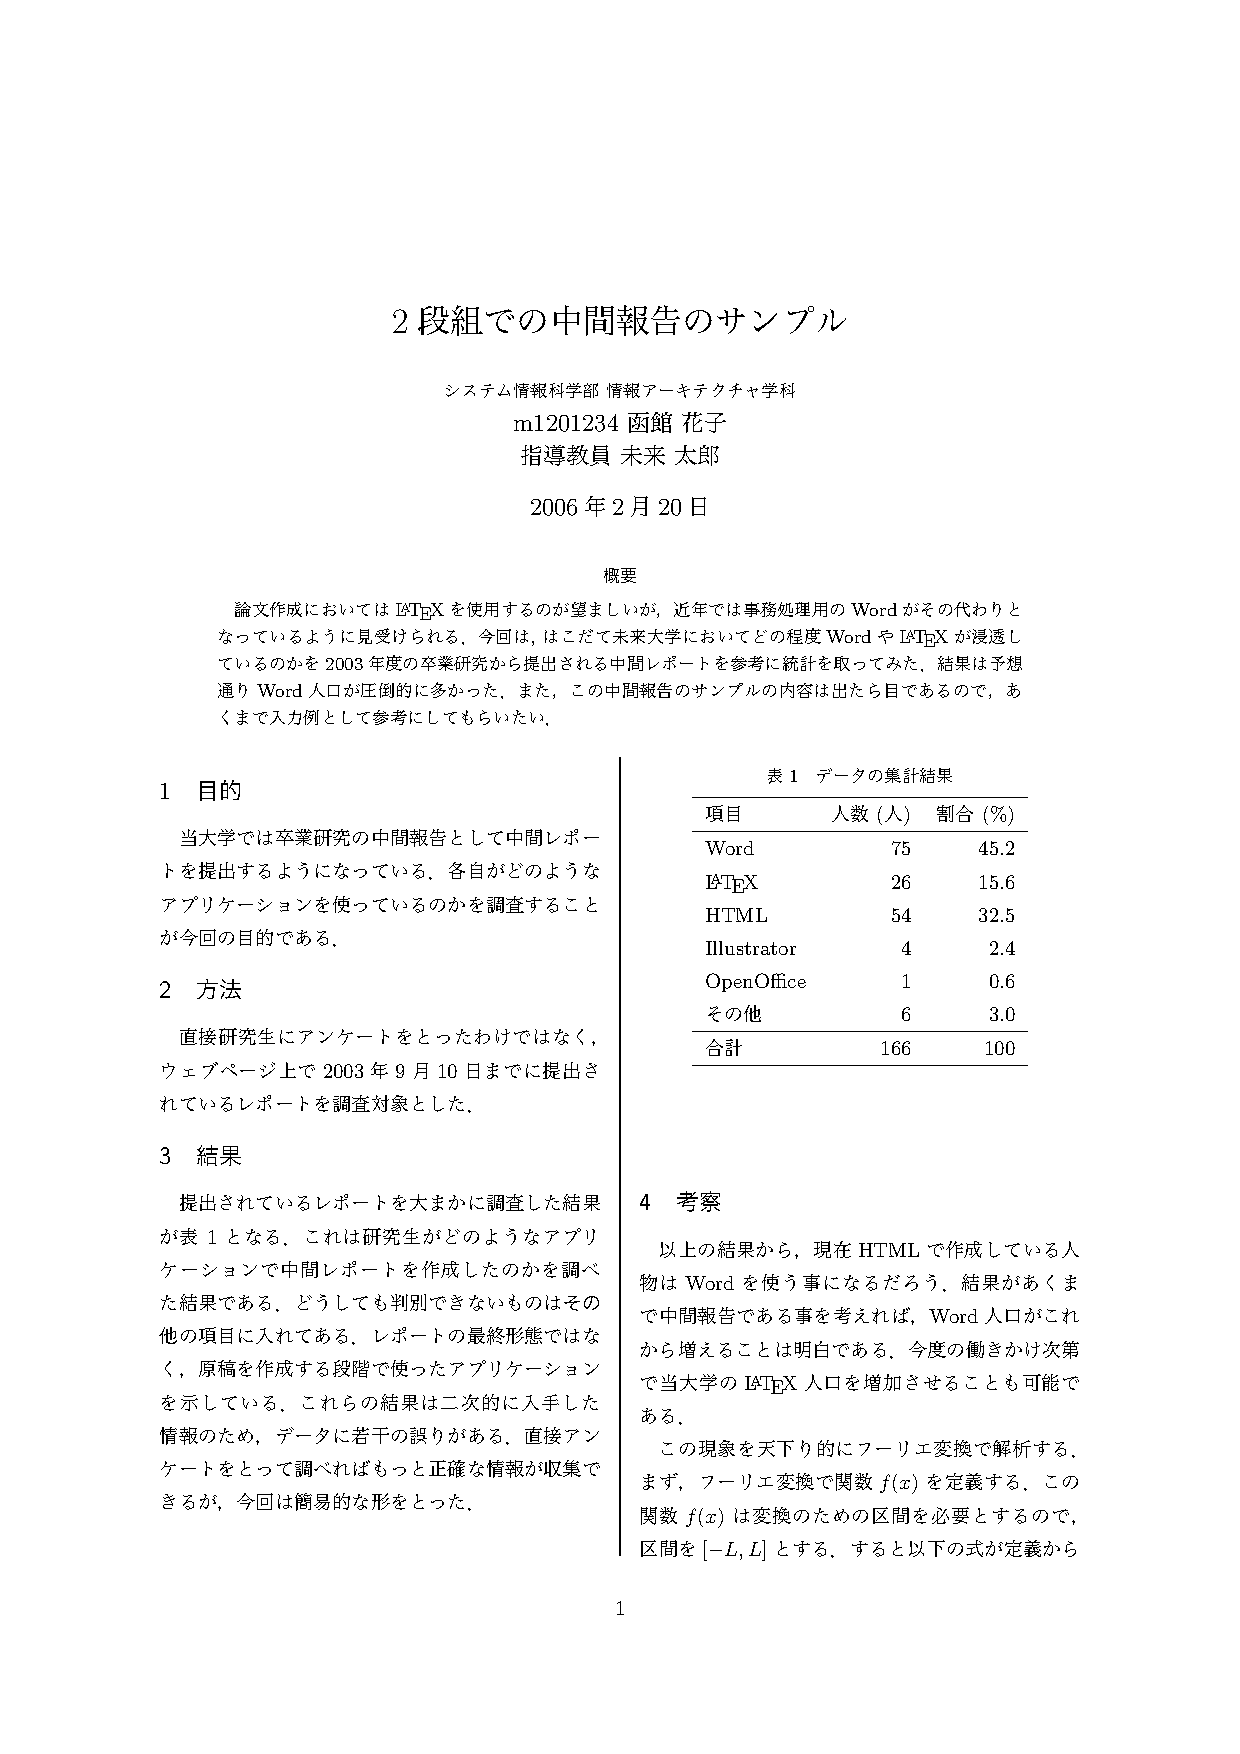
\includegraphics[width=\ftextwidth]{images/abst1}}
%\end{center}
%\clearpage
%\begin{center}
% \fbox{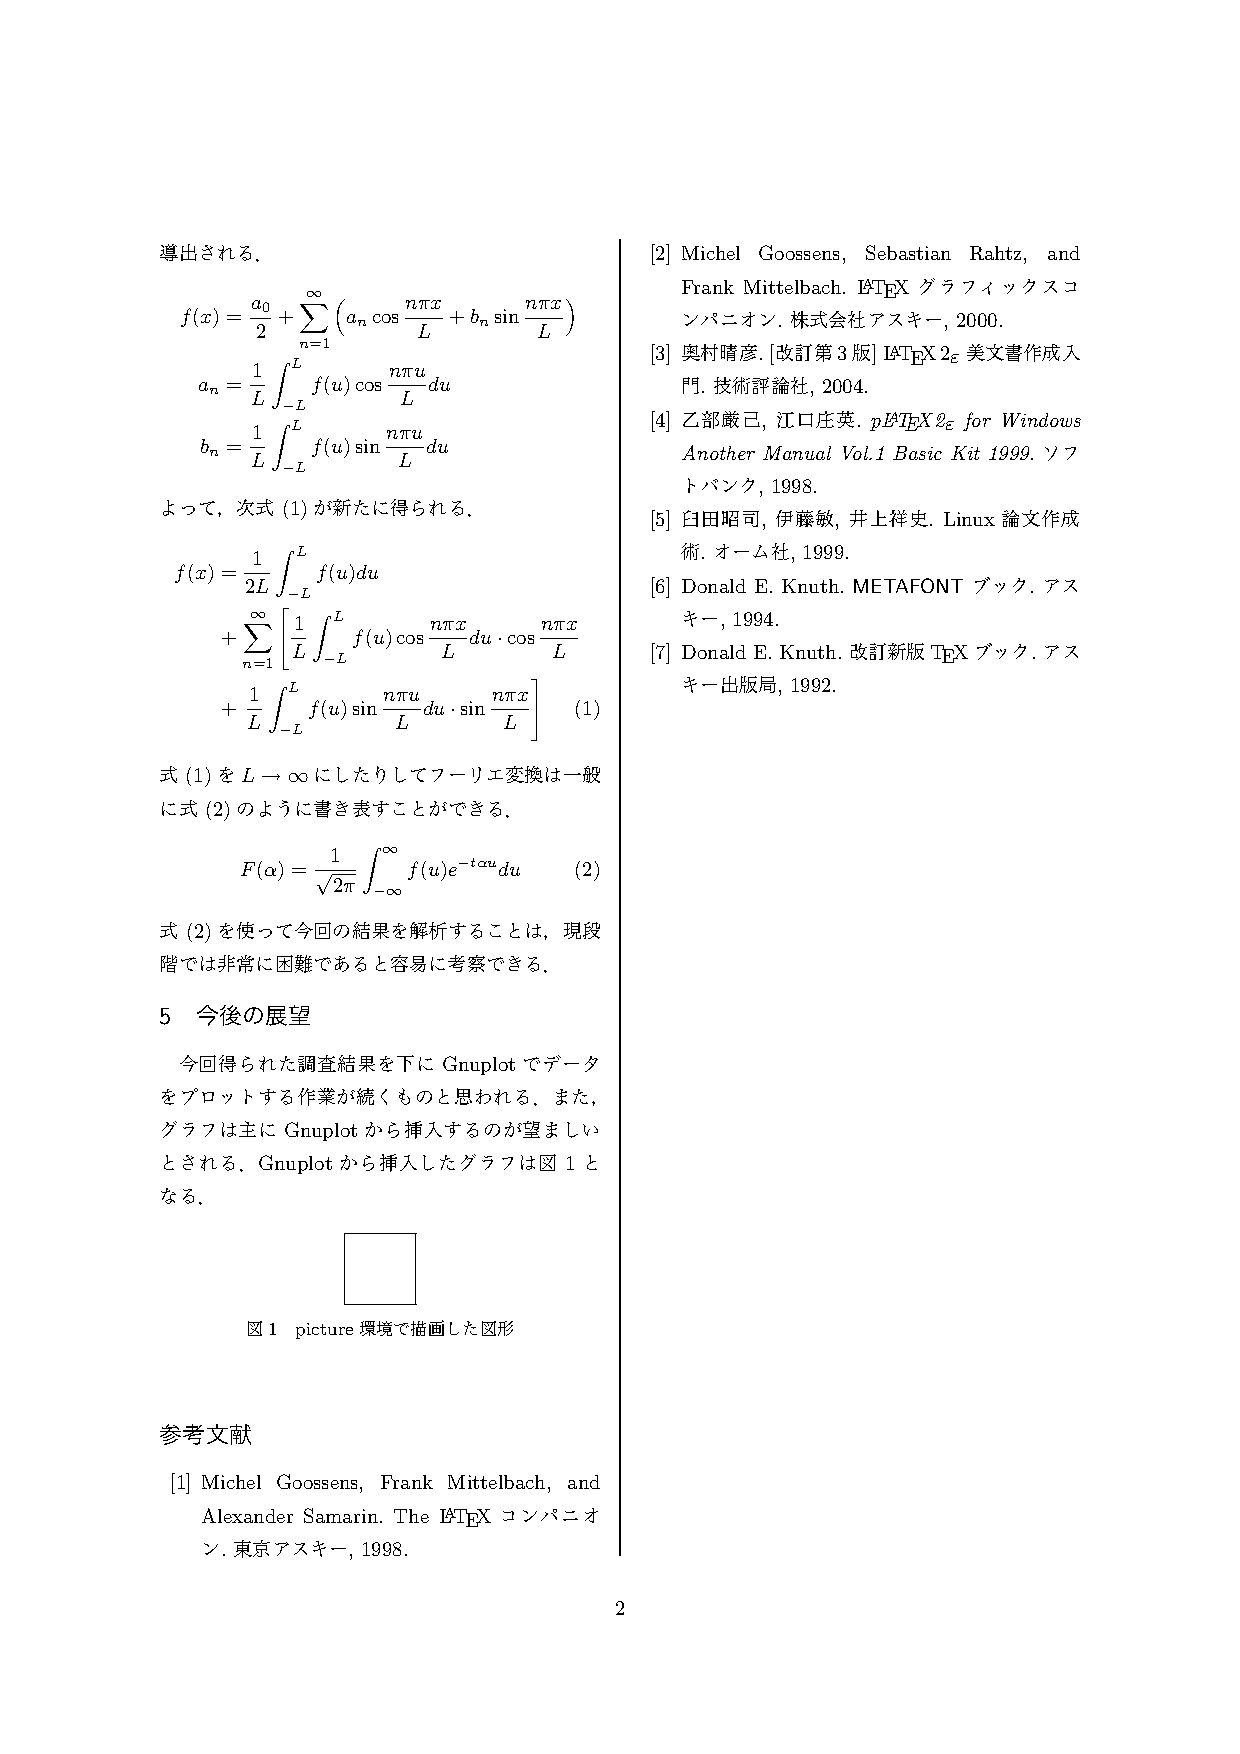
\includegraphics[width=\ftextwidth]{images/abst2}}
%\end{center}

\clearpage

\noindent \IOmargin \makebox[0pt][l]{%
\fbox{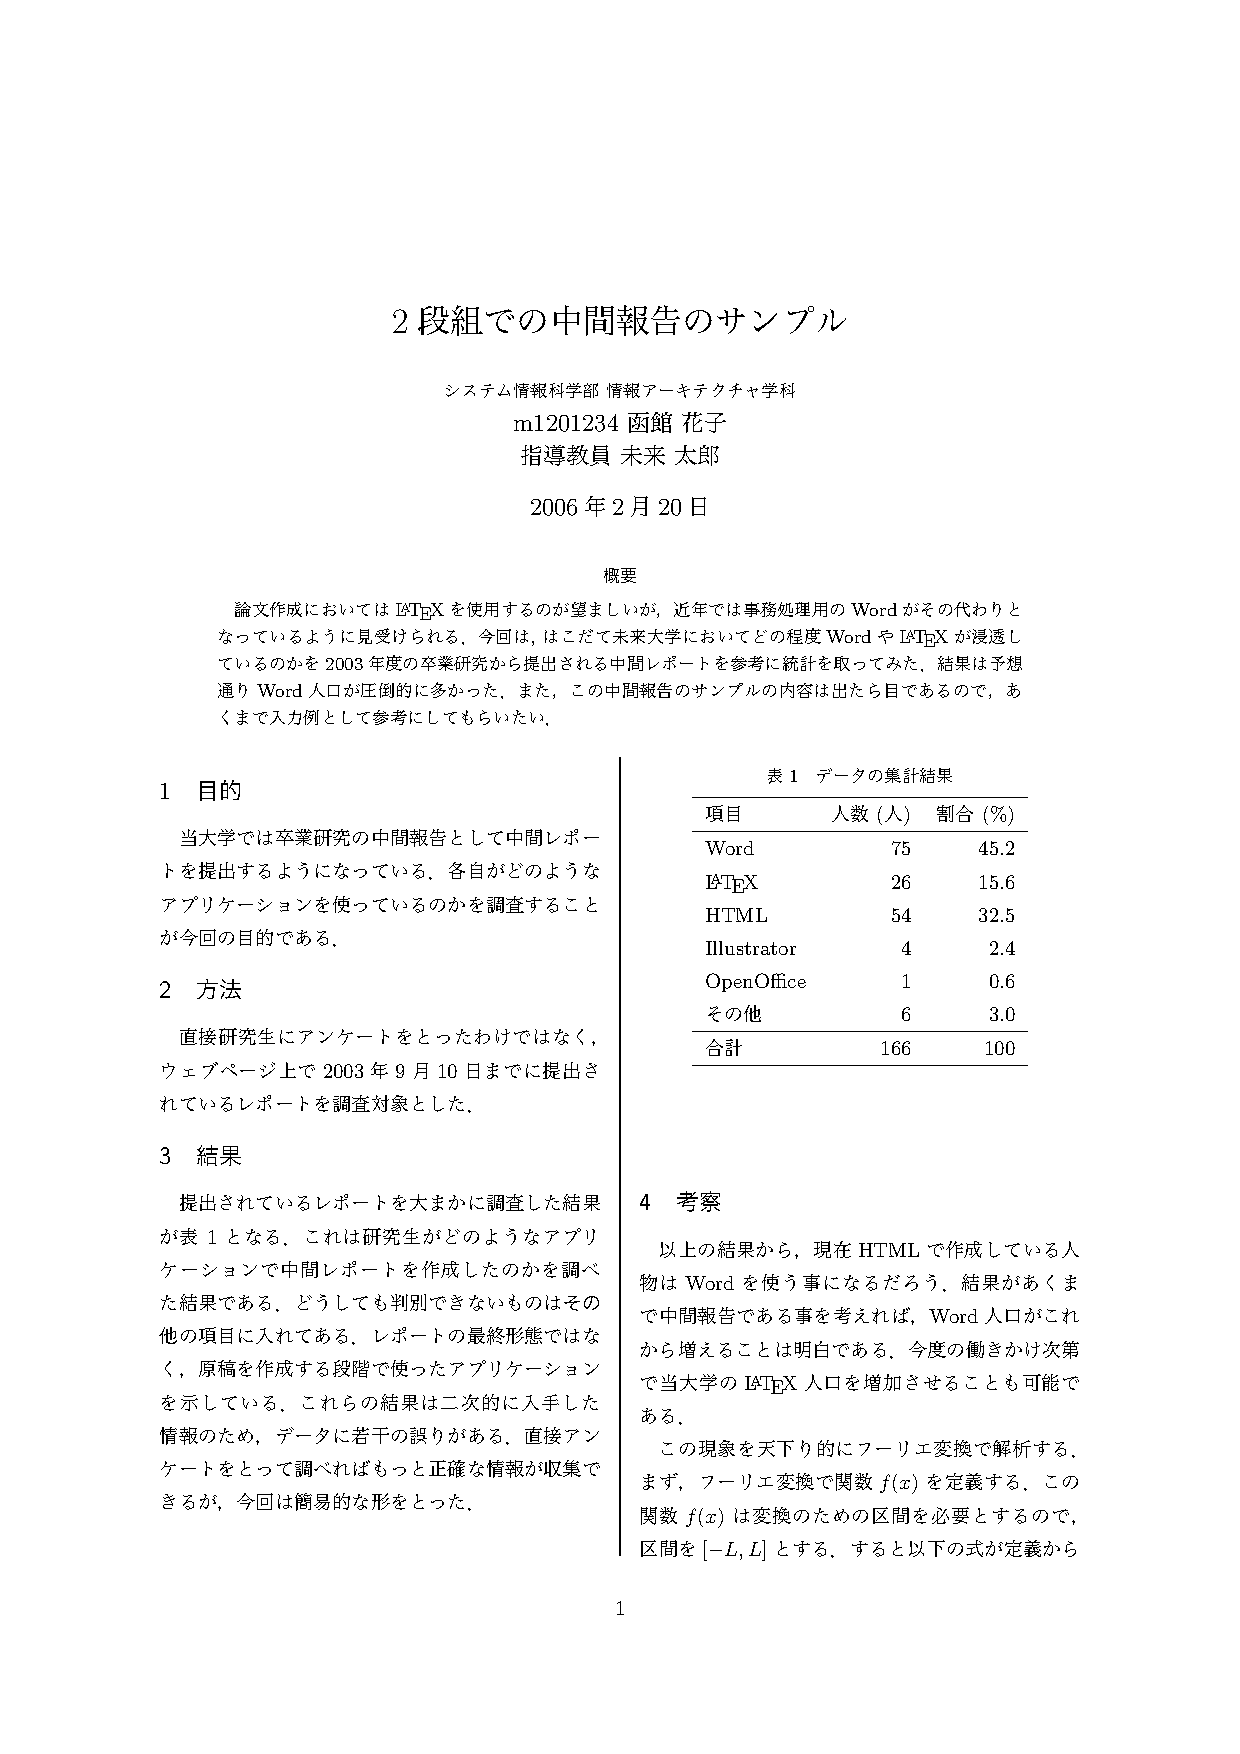
\includegraphics[clip,bb={0 0 595 842},width=\ffullwidth]
   {images/abst1}\IOlabel}}

\clearpage

\noindent \IOmargin \makebox[0pt][l]{%
\fbox{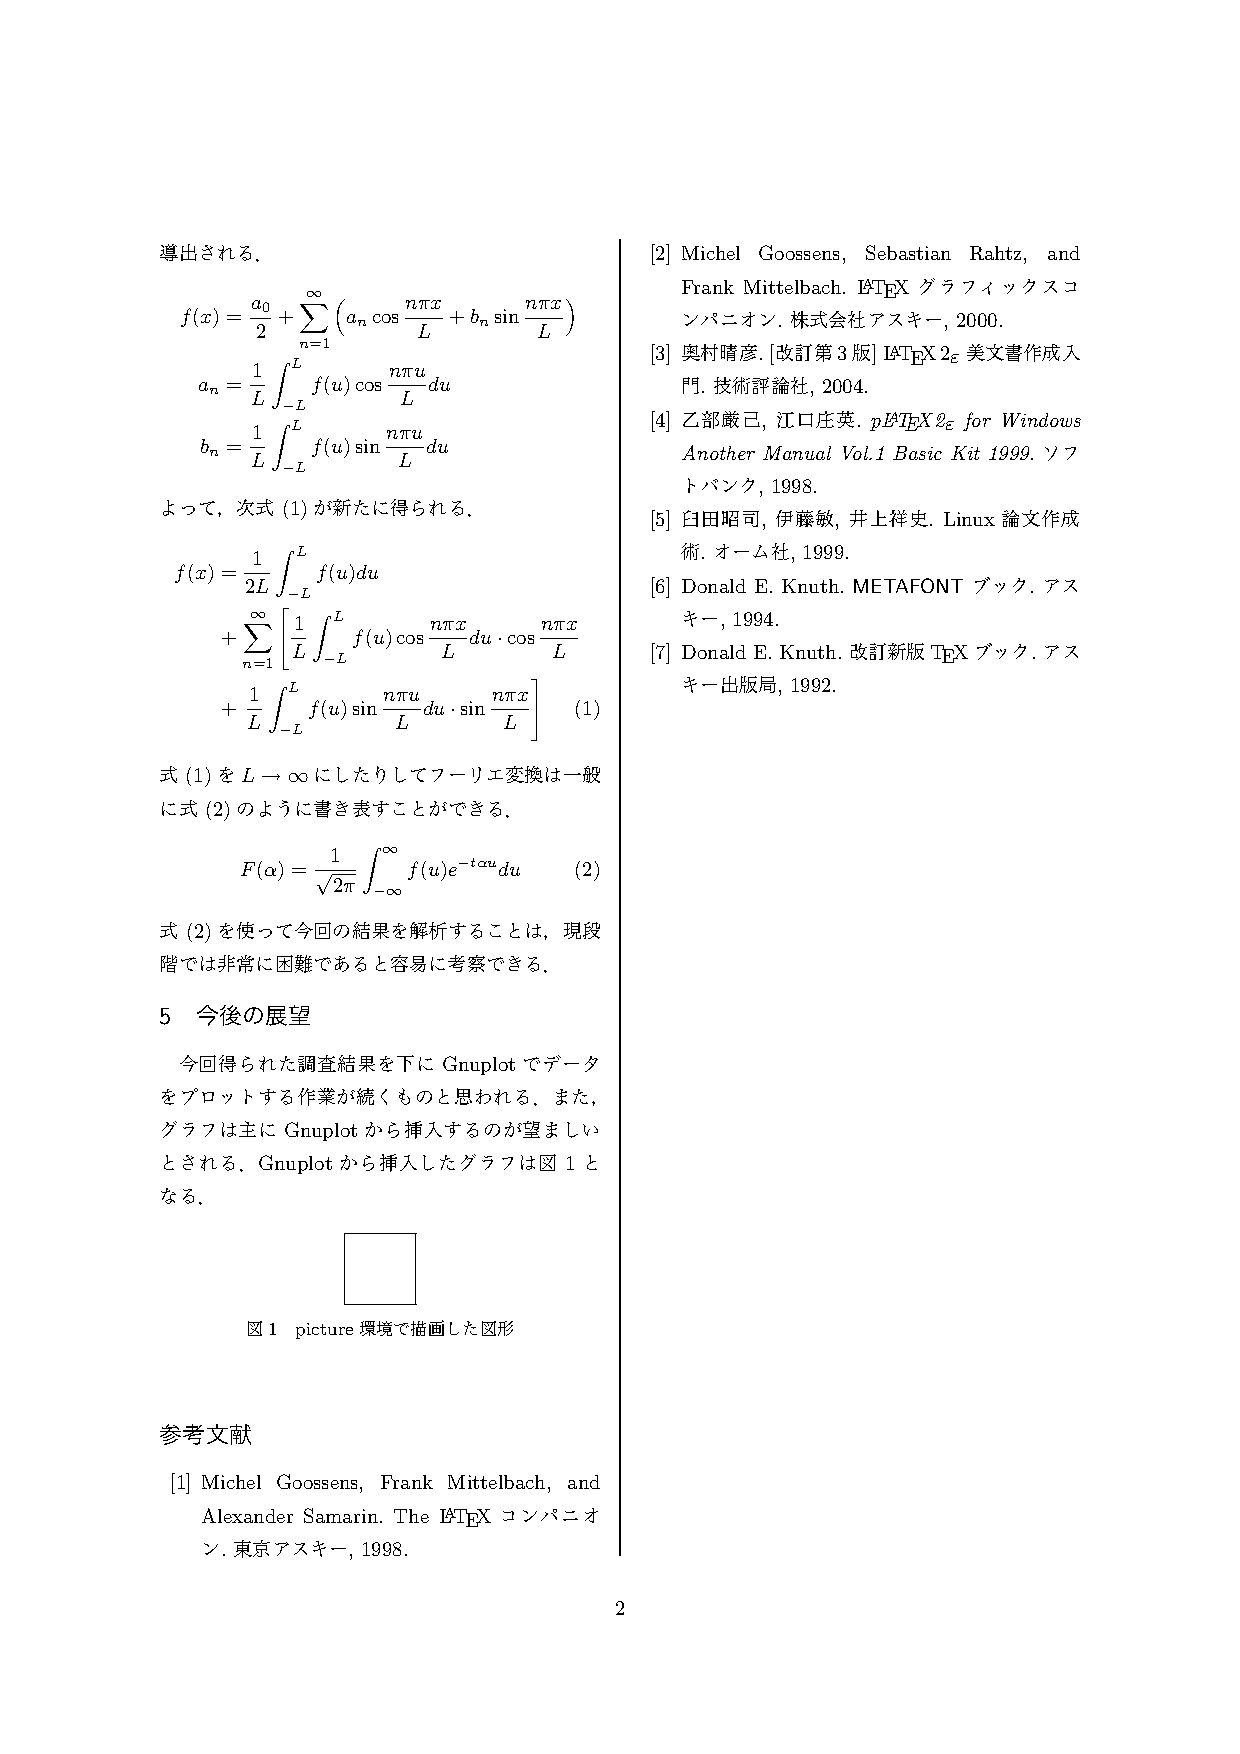
\includegraphics[clip,bb={0 0 595 842},width=\ffullwidth]
   {images/abst2}\IOlabel}}


\section{�ذ���ʸ�Υ���ץ�}

�ذ���ʸ�ʤɤϵ��ϤȤ����礭���ʤ�Τ�ʸ�񥯥饹��
\Cls{jreport}��\Cls{jsbook}��Ȥ����ˤʤ�Ȼפ��ޤ���

\cls{jsbook}�ξ��˥��饹���ץ�����
���Τ褦�ˤ���Ⱥ����������򤻤������̰����ǽ��Ϥ���ޤ���

\begin{InTeX}
\documentclass[11pt,report]{jsbook}
\end{InTeX}

\cls{jreport}��\cls{jsbook}�ǻ��ѤǤ��븫�Ф�
�� \C{chapter},  \C{section},  \C{subsection}
�λ��ĤǤ���\Cmd{subsubsection}̿��Ϥʤ�٤��Ȥ�ʤ��ۤ�
���ɤ��Ǥ��礦��\cls{jsarticle}ʸ�񥯥饹�ǻ��ѤǤ���
\env{abstract}�Ķ��ϻȤ��ʤ��ʤ�ޤ��Τ�
���Τ褦�ˤ���\Z{��Ω��}���ޤ���

\begin{InTeX}
\chapter*{����}\addcontentsline{toc}{chapter}{����}
�����˴ʷ�˳��פ�񤯡�
\end{InTeX}




\subsection{���饹�ե����뤬�󶡤���Ƥ�����}

�ذ���ʸ�ʤɤ����¦����ʸ�񥯥饹���󶡤�����������ޤ���
%����ؤ�´����ʸ�ξ���\Cls{funthesis}�Ȥ������饹�ե�����
%�����ۤ���Ƥ��ޤ��ΤǤ����Ȥ����Ȥˤʤ�ޤ���
%���饹�ե�����Ȥ���\cls{funthesis}��Ȥä���򼨤��ޤ���
%���ϤϾ�ά�����Ƥ��������ޤ���

\begin{InTeX}
%\documentclass[english]{funthesis}%��ʸ���Ѹ�ΤȤ�
\documentclass{funthesis}
\usepackage[dvipdfmx]{graphicx}%dvips�ξ���`dvips'�ˤ���
% ���ܸ����̾
% Ĺ���Ȥ���`\\'�Dz���
\jtitle{��Ω�Ϥ�����̤����ؤˤ�����´����ʸ��
{\LaTeX}���饹�ե�������߷פ˴ؤ���ͻ�}
% ��ʸ�α�ʸ�����ȥ�
\etitle{Title in English}
% ��̾(���ܸ�)
\jauthor{̤�� ��Ϻ}
% ��̾(�Ѹ�)
\eauthor{Taro MIRAI}
% ��°�ز�̾
\affiliciation{ʣ���ϥ������ƥ�����ز�}
% �����ֹ�
\studentnumber{1300000}
% ����Ƴ����̾
\advisor{����Ƴ ����}
% ����Ƴ������������ϥ����ȥ����Ȥ�̾�����
% ����Ƴ���������ʤ����ϡ������Ϻ�����Ƥ��
%\coadvisor{����Ƴ ����}
% ��ʸ�����
\date{2004/01/31}
%����������ʸ�λϤޤ�
\begin{document}
% ɽ��
\maketitle
%�Ѹ�γ���
\begin{eabstract} Abstract in English. (about 500 words)
\fake{you should write your English abstract in one page. }
% ��ʸ�������
\begin{ekeyword}
Keyrods1, Keyword2, Keyword3, Keyword4, Keyword5
\end{ekeyword}
\end{eabstract}
% ��ʸ����(2000������)
\begin{jabstract} ���ܸ�γ��פ�񤯡�(��200����
\fake{���������ܸ�γ��פ�񤭤ޤ���}
% ��ʸ�������
\begin{jkeyword}
�������1, �������2, �������3, �������4, �������5
\end{jkeyword}
\end{jabstract}
% �ܼ�
\tableofcontents 
% ���ܼ�
\listoffigures
% ɽ�ܼ�
\listoftables
\chapter{����} % ��(chapter)�Υ����ȥ�
�����˽�����񤭤ޤ���
\section{�ط�} % ��(section)�Υ����ȥ�
�ʲ����طʡ���Ϣ����Ķ������������Ѥ˴ؤ��복�פ򵭽ҡ�
\chapter{�ͻ�}
�ͻ����ޤ�����
\section{ɾ�����}
�ɤä����ɤä����Ǥ���
\chapter{�����Ⱥ����Ÿ��}
�ɤ�����Ǥ�����
% �ʹߡ���Ͽ(��°����)�Ǥ��뤳�Ȥ򼨤�
\begin{appendix}
\chapter{���르�ꥺ��}
%��Ͽ����1(��Ϣ�����ʤ�)��ɬ�פ�����кܤ���
\section{���륢�르�ꥺ��}
%��Ͽ����2(��Ϣ�����ʤ�)��ɬ�פ�����кܤ���
\chapter{������������}
�ץ������Υ����������ɤʤɤ�Ǻܤ��ޤ���
\section{���륽����������}
������������뤢��ץ������\texttt{hoge.cpp}�Υץ������򼨤���
\begin{verbatim}
int main( void ){ return 0; }
\end{verbatim}
\fake[40]{{\thehoge}��\par}
%��Ͽ�ν����
\end{appendix}
\chapter*{�ռ�}
�ռ���񤯡�
% ����ʸ��
\begin{thebibliography}{9}
 \bibitem{��٥�} ����̾. ����̾. ���Ǽ�, ǯ��.
 \bibitem{MT1999} ̤����Ϻ. ̤���̤��. �ɤ����ν���, 1999. 
\end{thebibliography}
\end{document}
\end{InTeX}
%

\subsection{���饹�ե����뤬�󶡤���Ƥ��ʤ����}

�⤷��ء�����¦���饯�饹���󶡤���Ƥ��ʤ����ϼ����Ǻ�������
���ˤʤ�ޤ�������ξ���Times�ϤΥե���Ȥ�Ȥäƥե���ȥ������ϲ���
�ǤȤ����٤�������򤷤Ƥ���Τ����̤Τ褦�Ǥ������ڤ��������Ǥ˺������ƥ���
�֤Ǹ������Ƥ���Ƥ�����⤢��ޤ���

�Ȥꤢ�����Ҷ����ޤ��Ǥ���\Cls{jsbook}���Ѥ������Ҳ𤷤ޤ���
\cls{jreport}��ȤäƤ��ɤ��Ǥ���\cls{jsbook}�������Ŀ�Ū�ˤ�
�ɤ��ȴ����Ƥ��ޤ����ޤ��Ϥ���ʬ����С������ε���˹�碌��
\cls{jsbook}������Τ����Ĥ����ѹ���ä��ޤ���\cls{jsbook}
���Τ�Τ��ѹ���ä���Ȥɤ��ˤɤΤ褦���ѹ���ä����Τ���ʬ��
��ʤ��ʤ�����ʤɤ�����ޤ��Τǡ��̥ե�����\fl{mygs.sty}���ѹ�
�����ޥ����ʤɤ�ޤȤ�Ƥ����ޤ����ե��������Ƭ��
���Τ褦�ʥե���������񤭹���Ǥ������ɤ��Ǥ��礦��

\begin{InTeX}
%% File: mygs.sty
%% Copying : Your Name
%% E-mail  : name@univ.ac.jp
%% Date    : 2006/04/20
\ProvidesPackage{mygs}[2006/04/20 First Family]
\end{InTeX}


����ε��ؤǤ�\Z{Times}�ϤΥե���Ȥ���ꤹ��Ȼפ��ޤ��Τ�
����1�Ԥ⤢����ɤ��Ǥ��礦��

\begin{InTeX}
\RequirePackage{txfonts}
\end{InTeX}

�ޥ����ѥå����������¾�Υѥå�������
ɬ�פȤ������ \C{Requirepacakge} ̿���Ȥ��ޤ���

���˥ڡ����쥤�����ȤˤĤ��ƤǤ����ޡ�����ˤĤ��Ƥ�٤���
����򤷤Ƥ��뤫�⤷��ޤ��󤬡������������ˡ��Ҳ𤷤ޤ��礦��
�ڡ����쥤�����Ȥ�����Ǥ�����ܤˤĤ��Ƥ�\figref{pagelayout}
�򸫤Ƥ����������ޤ���1�Ԥλ����Ǥ���1��40ʸ���Ǥ��ä��Ȥ����
Ĺ�� \Cmd{textwidth}������40ʸ������\pp{40zw}����ꤷ�ޤ���

\begin{InTeX}
\setlength\textwidth{40zw}
\setlength\fullwidth{\textwidth}%jsbook��ɬ��
\end{InTeX}

�Կ���40�ԤȻ��ꤵ��Ƥ���ΤǤ���С� \Cmd{textheight}��40\Z{������}
ʬ��Ĺ�� \pp{40\Cmd{baselineskip}} ����ꤷ�ޤ���

\begin{InTeX}
\setlength\textheight{40\baselineskip}
\end{InTeX}

�������٤Ǥ��ɤ��Ȼפ��ΤǤ������ڡ����쥤�����Ȥ�����򤷤Ƥ��ɤ��Ǥ��礦��

\C*{hoffset}%
\C*{voffset}%
\C*{evensidemargin}%
\C*{oddsidemargin}%
\C*{topmargin}%
\C*{headheight}%
\C*{headsep}%
\C*{marginparwidth}%
\C*{marginparpush}%
\C*{marginparsep}%
\begin{InTeX}
\setlength\hoffset{13\p@}
\setlength\voffset{0\p@}
\setlength\evensidemargin{0\p@}
\setlength\oddsidemargin{\evensidemargin}
\setlength\topmargin{0\p@}
\setlength\headheight{0\p@}
\setlength\headsep{0\p@}
\setlength\marginparwidth{0\p@}
\setlength\marginparpush{0\p@}
\setlength\marginparsep{0\p@}
\end{InTeX}

�����Ǥ� \C{p@} ��
ñ��\qu{pt}�λ��Ǥ����ޥ�������ǤϤ��Τ褦��̿���Ȥ�����
�������Ǥ��������Ǥ�˵����إå�������Ϥ��ʤ��Ȳ��ꤷ��
�ۤȤ�ɤι��ܤ�\qu{0pt}���������Ƥ��ޤ���

�إå�����եå����ϳ�ȥ���ץ�ʤ�Τ��ɤ��Ȼפ��Τ�
\cls{jsbook}�ξ��ϥեå���������˥ڡ����ֹ����Ϥ���褦�ˤ��ޤ���

\begin{InTeX}
\pagestyle{plainfoot}
\end{InTeX}

\cls{jreport}�Ϻǽ餫�饷��ץ��\str{plain}�Ȥ���
�ڡ�����������ˤʤäƤ��ޤ���
��������\qu{-- 13 --}�Τ褦�˥��å���������Ȥ���
���Τ褦�ˤ��ޤ���

\zindind{����}{�Υڡ����ֹ�}%
\C*{footskip}%
\C*{baselineskip}%
\begin{InTeX}
 \let\@mkboth\@gobbletwo
 \let\@oddhead\@empty
 \let\@evenhead\@empty
 \def\@oddfoot{\normalfont\hfil-- \thepage\ --\hfil}%
 \let\@evenfoot\@oddfoot
 \setlength\footskip{2\baselineskip}%ɬ�פ˱�����
\end{InTeX}

�ڡ����ֹ�������ˤ���Ȥ��� \C{normalfont}
�θ�� \Cmd{bfseries}���ɲä��ޤ���

%���Ф��Υե���Ȥξ�����ʸ�ϥ����å�����ʸ��Times Bold
���Ф��Υե���Ȥ���ʸ�򥴥��å�����ʸ��Times Bold�ˤ������Ȥ���
\cls{jsbook}�ξ��ϼ��Τ褦�ˤ��Ƥ������ɤ��Ǥ��礦��

\begin{InTeX}
\renewcommand{\headfont}{\gtfamily\rmfamily\bfseries}
\end{InTeX}

\cls{jsbook}��ɸ���
�ϲ�ʸ�����󥻥���ΤˤʤäƤ��ޤ���\cls{jreport}�ξ��
�Ϻǽ餫�鲤ʸ���ܡ�����Τ����ꤵ��Ƥ��ޤ���

���ޤ����ܼ��ο�������륫����\str{tocdepth}��
���Τ褦�ˤ���� \C{subsection} �ޤǽ��Ϥ���ޤ���

\begin{InTeX}
\setcounter{tocdepth}{2}
\end{InTeX}


\cls{jreport}�ξ��ϸ��Ф��θ�λ��������Ԥ��ʤ���������ޤ��ΤǼ�
�Τ褦�ˤ���\Sty{indentfirst}�ѥå��������ɤ߹��ߤޤ���

\begin{InTeX}
\RequirePackage{indentfirst} 
\end{InTeX}


������ޤȤ��ȼ�ʬ�Υޥ����ѥå�����\sty{mygs.sty}��
����夬��Ǥ�\footnote{\url{http://tex.dante.jp/jou1/mygs.sty}}��

\begin{InTeX}
%% File: mygs.sty
%% Copying : Thor Watanabe
%% E-mail  : thor@tex.dante.jp
%% Date    : 2006/04/20
\ProvidesPackage{mygs}[2006/04/20 First Family]
\RequirePackage{txfonts}% Times�ϤΥե���Ȥ�Ȥ�
%\RequirePackage{indentfirst}% jreport��ɬ��
\setlength\textwidth{40zw}%1��40ʸ��
\setlength\fullwidth{\textwidth}%jsbook�Ǥ�ɬ��
\setlength\textheight{40\baselineskip}%1�ڡ���40��
\setlength\hoffset{13\p@}%\p@��0pt����
\setlength\voffset{0\p@}
\setlength\evensidemargin{0\p@}
\setlength\oddsidemargin{\evensidemargin}
\setlength\topmargin{0\p@}
\setlength\headheight{0\p@}
\setlength\headsep{0\p@}
\setlength\marginparwidth{0\p@}
\setlength\marginparpush{0\p@}
\setlength\marginparsep{0\p@}
\setlength\footskip{2\baselineskip}%ɬ�פ˱�����
\def\ps@foot{%�եå����� `-- �ڡ����ֹ� --'�Ȥ������Ȥ�
 \let\@mkboth\@gobbletwo
 \let\@oddhead\@empty
 \let\@evenhead\@empty
 \def\@oddfoot{\normalfont\hfil-- \thepage\ --\hfil}%
 \let\@evenfoot\@oddfoot
}
\pagestyle{plainfoot}%jsbook�ʤ��
%\pagestyle{plain}%jreport�ʤ��
\renewcommand{\headfont}{\normalfont\bfseries}
\setcounter{tocdepth}{2}
\end{InTeX}

���Τ褦�ʺ�Ȥ�����ä��鼫ʬ����ʸ�μ�Ȥʤ륽�����ե�����
��񤭾夲�ޤ����ѻ��A4�ǡ��ե���ȥ�������11\,pt������������
�Ϥ��������̰����Ȥ����Τ�����Ū���Ȼפ��ޤ����鼡�Τ褦�ˤ��ޤ���

\begin{InTeX}
\documentclass[a4j,11pt,report]{jsbook}
\end{InTeX}

������������������\fl{mygs.sty}�� \C{usepackage}̿����ɤ߹��ߤޤ���

\begin{InTeX}
\usepackage{mygs}
\end{InTeX}


�������٤Ǥ��ɤ��ΤǤ�����ɽ���ޤ��٤�������򤵤����
������ޤ���1���� \cmd{maketitle}���äƤ��ɤ��ΤǤ�������
����᤯��ʸ��ž夲�ʤ���Фʤ�ʤ��Ȥ��ˡ�̿����������
�ϴ֤˹��ʤ������Τ�ޤ��󡥤��Τ褦�ʤȤ�����IJ�λפ�
�� \Cmd{titlepage}�Ķ�����Ѥ���ɽ��������Ǥ��ޤ���%
\indindz{ɽ��}{ɽ���}\index{ɽ��κ���}%
��Ȥ��� \Cmd{maketitle}̿����ѹ����Ҳ𤷤ޤ���

\C*{vskip}%
\C*{cvs}%
\C*{headfont}%
\C*{null}%
\begin{InTeX}
\renewcommand{\maketitle}{%
\begin{titlepage}
    \let\footnotesize\small
    \let\footnoterule\relax
    \let\footnote\thanks
    \null\vskip2\cvs%�ڡ��������ζ���
    \begin{center}\thispagestyle{empty}%
      {\LARGE\headfont ������ɽ���񤭤ޤ�}\par\vskip\cvs
      {\Large\normalfont ̤����Ϻ}\par\vskip2\cvs
      {\small ̤�踦��ز� \qquad �����ֹ�}\par\vskip.5\cvs
      {\small ��Ƴ���� \qquad �̳���Ϻ}\par\vskip2\cvs
      {����� 2006/03/30}\par\vskip3\cvs
      {\Large\headfont English Title}\par\vskip\cvs
      {\large\rmfamily Your Name}\par\vskip\cvs
    \end{center}%
    \vfill\null
\end{titlepage}}
\end{InTeX}

\C{vskip}�ȤϿ�ľ�����˶�������������̿��Ǥ���

�ʾ����Ǥ��Τ������˵��ꤵ�줿�̤�Υ쥤�����Ȥ�
Ŭ���ѹ����Ƥ���������



���Ф�����Ϥ��� \cmd{section} ̿����κۤ�Ŭ�ڤǤϤʤ���
�פ���ΤǤ���С�Ŭ�� \cmd{section}����̿����������ޤ���

\begin{Syntax}
\C{@startsection}\pa{���Ф��μ���}%
  \pa{����}\pa{������}\pa{������}\pa{�����}\\
\hskip3zw\pa{�κ�}\str*\opa{�ܼ��Ѥθ��Ф�}\pa{���Ф�}
\end{Syntax}

\begin{Exe}
�ºݤ� \fl{jsbook.cls}���� \cmd{section}������򲿤�����Υե�����˥��ԡ�
���Ƥ���������

\begin{InTeX}
\makeatletter
\renewcommand{\section}{%
    \if@slide\clearpage\fi
    \@startsection{section}{1}{\z@}%
    {\Cvs \@plus.5\Cdp \@minus.2\Cdp}% ������
    {.5\Cvs \@plus.3\Cdp}% �奢��
    {\normalfont\Large\headfont\raggedright}}
\makeatother 
\end{InTeX}

\cmd{newcommand} �� \cmd{renewcommand} ���ѹ����ޤ���
�����ǡ�\Cmd{raggedright}�ȤʤäƤ���ս�� \Cmd{centering}
�����ѹ�����ȷ�̤ϤɤΤ褦�ˤʤ뤫��̣���Ƥ���������
\end{Exe}

¾�ˤ�ϸ��Ф����κۤ� \C{@makechapterhead}, \C{@makeschapterhead}��
��ɽ���Ф����κۤ� \C{@makecaption}��ʸ�������Υ�٥���κ�
�� \C{@biblabel}�Ȥ������ˡ����줾���б����륳�ޥ�ɤ�¸�ߤ��ޤ���

\begin{Prob}
���ε��Ҥ��ɲä���� \C{section}����̿��ϤɤΤ褦���Ѥ��Ǥ��礦����

\begin{InTeX}
\renewcommand\@seccntformat[1]{\@nameuse{the#1}.\quad}
\end{InTeX}

�ºݤ˥����ץ��åȤ������Ϸ�̤��̣���Ƥ���������
% ñ�˸��Ф��κǸ�˥ԥꥪ�ɤ��դ��ޤ���
\end{Prob}

\begin{Prob}
�ϸ��Ф��ϼºݤ� \C{@makechapterhead} ̿���ɽ������ޤ���
7���ܤ�`\cmd{par}\C{nobreak}'��`\C{vskip} \C{Cvs}'�Ȥ������Ҥ�������
�Ȥɤ��ʤ�ޤ�����
�ޤ���\cmd{raggedright}�� \cmd{centering}�����ѹ�����ȤɤΤ褦��
���Ϸ�̤ˤʤ�Τ����ºݤ˥����ץ��åȤ��Ƴ�ǧ���Ƥ���������

\begin{InTeX}
\def\@makechapterhead#1{%
  \vspace*{2\Cvs}% ��ʸ��50pt
  {\parindent \z@ \raggedright \normalfont
    \ifnum \c@secnumdepth >\m@ne
      \if@mainmatter
        \huge\headfont \@chapapp\thechapter\@chappos
        \par\nobreak
        \vskip \Cvs % ��ʸ��20pt
      \fi
    \fi
    \interlinepenalty\@M
    \Huge \headfont #1\par\nobreak
    \vskip 3\Cvs}} % ��ʸ��40pt
\end{InTeX}

\end{Prob}

\begin{Prob}
\cls{jsclasses}��\env{quotation}�Ķ��Ǥϡ���;�� 0\,pt������
����Ƥ��ޤ�������Ǥ� \env{quotation}�Ķ��򲼵��Τ褦�˺��������ȡ�
��̤ϤɤΤ褦�ˤʤ�Τ����ºݤ˥����ץ��åȤ��Ƴ�ǧ���Ƥ���������

\begin{InTeX}
\renewenvironment{quotation}{%
  \list{}{%
    \listparindent\parindent
    \itemindent\listparindent
    \rightmargin = \leftmargin}%
  \item\relax}{\endlist}
\end{InTeX}
\end{Prob}

\begin{Prob}
��ɽ���Ф��� \C{@makecaption} �ˤ�ä�ɽ������Ƥ��ޤ���
�Ǥϡ�`\verb|\advance\leftskip1cm|'��`\verb|\advance\rightskip1cm|'�Ȥ���
���Ҥ�������ȷ�̤Ϥɤ��ʤ뤫���ºݤ˥����ץ��åȤ��Ƴ�ǧ���Ƥ���������

\begin{InTeX}
\long\def\@makecaption#1#2{{\small
  \advance\leftskip1cm
  \advance\rightskip1cm
  \vskip\abovecaptionskip
  \sbox\@tempboxa{#1\hskip1zw\relax #2}%
  \ifdim \wd\@tempboxa <\hsize \centering \fi
  #1\hskip1zw\relax #2\par
  \vskip\belowcaptionskip}} 
\end{InTeX}
\end{Prob}

\begin{Prob}
�ܼ���ˤ�����ϸ��Ф��� \C{l@chapter}��ɽ������ޤ���
�Ǥ� \C{begingroup}�θ�� \C{large}�򵭽Ҥ���Ȥɤ��ʤ뤫��
�ºݤ˥����ץ��åȤ���������ǧ���Ƥ���������

\begin{InTeX}
\renewcommand*{\l@chapter}[2]{%
  \ifnum \c@tocdepth >\m@ne
    \addpenalty{-\@highpenalty}%
    \addvspace{1.0em \@plus\p@}
    \begingroup
      \parindent\z@
      \rightskip\@tocrmarg
      \parfillskip-\rightskip
      \leavevmode \large \headfont % ������ \large ���ɲ�
      \setlength\@lnumwidth{4.683zw}%
      \advance\leftskip\@lnumwidth \hskip-\leftskip
      #1\nobreak\hfil\nobreak\hbox to\@pnumwidth{\hss#2}\par
      \penalty\@highpenalty
    \endgroup
  \fi} 
\end{InTeX}
\end{Prob}



%\begin{table}[htbp]
% \begin{center}
%  \caption{�Ƽ�ز����ʸ����ѥ��饹���ޥ���}\tablab{gakkai}
% \begin{tabular}{ll}
% \egakkai{IEEE}
% \gakkai{���������ǥ���}
% \gakkai{��¬��ư����}
% \gakkai{�������}
% \gakkai{�����ƥ��������}
% \gakkai{�͹���ǽ}
% \gakkai{��̩��}
% \gakkai{�ŵ�}
% \gakkai{�ŻҾ����̿�}
% \gakkai{�ҥ塼�ޥ󥤥󥿥ե�����}
% \gakkai{���ܲ���}
% \gakkai{���ܷ�¬��}
% \gakkai{���ܵ���}
% \gakkai{���ܥ��եȥ�������}
% \gakkai{���ܥ��ܥå�}
% \gakkai{���ܥ��ڥ졼����󥺥ꥵ����}
% \gakkai{���ڳز�}
% \gakkai{���ܿ�����}
% \gakkai{���ܿ�������}
% \gakkai{��������}
% \gakkai{�ץ饺�ޡ���ͻ��}
% \gakkai{���ܿ��в�ϩ}
% \end{tabular}
% \end{center}
%\end{table}

%   9 書式のサンプル
\appendix%
\begin{small}%
%#!platex jou.tex
\chapter{�Ƕ��ư��}\applab{future}

% Many thanks to *crazy* TeXnicians and TeXperts.
\begin{abstract}
 \TeX ��������Ǯ��Ū���������ơ��β��ɤ並��򤵤�Ƥ���Τǡ�������
 �⤷�Ƥ��ޤ��������γ�ȯ��ȯŸ��ƨ���Ƥ���ȡ����ä��������ʥץ������
 ��ѥå���������������Ƥ��ʤ����ä����ʤ����ˤʤ꤫�ͤޤ��󡥤Ǥ����顤
 ���Υڡ����Ǥϼ��\genzai  \TeX ���դ�ȯŸ���Ƥ��������ʥġ����ѥ�
 ��������Ҳ𤷤ޤ���
\end{abstract}


\section{PDF ��\TeX}

\TeX �Ȥ����Τ� \Person{Donald}{Knuth} �Ȥ���\Z{�׻����ʳؼ�}������ǯ����
�˳�ȯ�����ץ������Ǥ��Τǡ���ʬ����ˤ�����ʤ���ʬ������Ȼפ��ޤ���
������ \TeX ����ɤ��� \Prog[eTeX]{\eTeX} �ʤ��Τ���ȯ����Ƥ��ޤ���
\TeX �Υ쥸�����������䤷���ꡤ�����ȿ��������ޥ�ɤ��ɲä��Ƥ��������
���ʤΤǤ�����\genzai ���ܸ첽����Ƥ��ޤ���\footnote{�����Ĥ��Υ��ץ���
�������ܸ�򰷤���ߤϤ��Ǥˤ���ޤ����������ʳ��ˤޤ�ã���Ƥ��ʤ��Τ�����
�Ǥ���}��

% H\`an Th\'{\^e} Th\`anh �ʥϥ󡦥���������ˡ��٥ȥʥ�� TeXnician
%\url{http://www.tug.org/tug2003/bulletin/souvenirs/photos/TUG2003-Day4-WednesdayJuly23/TUG2003-Day4-WednesdayJuly23-Images/11.jpg}
����� \TeX ����ľ�� PDF �ե����������������Ȥ����Τ���˾�Ȥ��Ƥ���Τ�
�������ºݤ� \Person{H\`an Th\'{\^e}}{Th\`anh}��ˤ�� \Prog[PDFTeX]{\PDFTeX} ��
\Prog[PDFlatex]{\PDFLaTeX} �Ȥ����ץ�����ब¸�ߤ��ޤ�������ϥե����
��ȥꥯ���ȼ¥ե���ȡʤޤ��ϲ��ۥե���ȡˤ�ξ���˥�������������ǰ쵤
�� PDF ���������Ȥ�����ΤǤ���\genzai ���ܸ첽����Ƥ��ޤ���

\index{LaTeX 3@\LaTeX\,3}%
����� \eTeX �� \PDFTeX ��ޡ������� \Prog[PDFeTeX]{\PDFeTeX} �Ȥ����Τ�
���ޤ�Ƥ��ޤ���������� \Prog[PDFeLaTeX]{\PDFeLaTeX} �⤢��ޤ����ᤤ��
�� \LaTeXe �θ�ѥС������Ǥ��� \LaTeX\,3 ���о줹��Ǥ��礦����
\eTeX/\PDFTeX �����ܸ첽���������ᤤ�Ȼפ��ޤ���

\zindind{Mac OS X}{��ATSUI}%
\Z{Mac OS X}�δĶ��˰�¸���ޤ�����\PDFeTeX ��١����ˤ���
\Prog[XeTeX]{\XeTeX}\footnote{\webXeTeX}�Ȥ����ץ������⤢��ޤ�������� Mac~OS~X ��
\Z{ATSUI}: Apple Type Services for Unicode Imaging ��ľ�ܥ�����������
�����ƥ�Υե���Ȥ����ѤǤ���褦�ˤʤ��ΤǤ���

\section{ʸ���Ƚ���}\seclab{app:typeface}

% Young U. Ryu. utdallas��ؤ� TeXnician. PXFonts/TXFonts �Ϥ⤦�����Ϥ�
% ����Ȥ��ơ����γ�ȯ����Ϥ��Ǥ˼������Ƥ��롥�����Ĥ��ΥХ����Ĥ����
% ����Τ����ˤʤ롥
\TeX �Ǥ�ɸ��Ū��\person{Donald}{Knuth}�ˤ��\Z{Computer Modern}�ե����
�Τߤʤ餺���͡��ʽ��Τ�Ȥ������Ǥ���褦�ˤʤäƤ��Ƥ��ޤ���Computer
Modern�ե���Ȥ�\PS\ Type 1 ������ PDF �� \PS �������ߤǤ���
\Y{type1cm} �ѥå�����������ޤ��������\Z{�衼���åѸ��}��\Z{��������
�ȵ���}��ޤ� \Y{type1ec} �ѥå�������ͭ�ѤǤ���
\Z{Times} �Ϥν��Ρ�\Prog{Word} ��ɸ��Ǥ⤢��ˤ���ʸ�˻Ȥ������ʤ��
\Person{Young}{Ryu}�ˤ��\Y{txfonts}��\Z{Palatino}�Ϥν��Τʤ��
\Y{pxfonts}���Υѥå������������Ǥ���\figref{basic:font:change}�ˡ�

\begin{table}[htbp]
 \begin{center}
  \caption{�ե���ȴ�Ϣ�Υѥå���������}\tablab{fontpac}
  \begin{tabular}{lp{65pt}llll} 
   \TR
   \Th{�ѥå�����}  & \Th{�����ޥ�}   & \Th{���󥻥��}   & \Th{�����ץ饤��} 
    & \Th{����}\\
   \MR
   % European Computer Modern: cm-super ec tc tt2001
   % European Modern: EM (PS)
   % Latin Modern LM (PS)
   % cm blue sky (PS), cm bakoma (PS, trutype), cm (Metafont)
   % �������ޤ��ͤù��ޤʤ���
   ����ʤ�    & CM~Roman & CM~Sans~Serif & CM~Typewriter & CM~Roman\\
   \Y{pxfonts} & Palatino�� & Helvetica��  & Monospaced��   & Palatino��\\
   \Y{txfonts} & Times��    & Helvetica��  & Monospaced��   & Times��\\
   \Y{lmodern} & LM~Roman & LM~Sans~Serif & LM~Typewriter & \\
   % Latin modern fonts in type 1 format based on the Computer Modern fonts
   % ��������\usepackage[T1]{fontenc}ɬ��
   \Y{type1cm} & CM~Roman & CM~Sans~Serif & CM~Typewriter & \\
   % ��������\usepackage[T1]{fontenc}�λ��� type1ec �ߴ�
   \Y{type1ec} & EC~Roman & EC~Sans~Serif & EC~Typewriter & \\
   % Computer modern fonts in T1 and TS1 encodings.
   \MR
   \Y{mathptmx}& Times      &              &                & Times \\
   \Y{mathpazo}& Palatino   &              &                & Palatino\\
   \Y{helvet}  &            & Helvetica    &                & \\
   \Y{avant}   &            & Avant Garde  &                & \\
   \Y{courier} &            &              & Courier        & \\
%   \Y{chancery}& Zapf~Chancery &           &                & \\
   \Y{bookman} & Bookman    & Avant Garde  & Courier        & \\
   \Y{newcent} & \hbox to 64pt{New~Century\hfil} Schoolbook & 
           Avant Garde & Courier & \\
   \Y{charter} & Charter    &              &                & \\
%   \Y{pifont}  & & & \\
%   \Y{mathptm} & Times & &  & Times\\%obsolete
%   \Y{mathppl} & Palatino & &  & Palatino\\%obsolete
%   \Y{times}   & Times      & Helvetica    & Courier        & \\%obsolete
%   \Y{palatino}& Palatino   & Helvetica    & Courier        & \\%obsolete
   \BR
  \end{tabular}
 \end{center}
\end{table}

\begin{figure}[htbp]
% \begin{center}
\newcommand*\mathimage[2][clip]{%
  \noindent\hbox{%
    \fbox{\includegraphics[#1]{mathFontTest/smpl-#2-crop}}\space
    {\sty{#2}}%
  }\par%
}%
  \mathimage[bb=0 0 189 95]{type1cm}%
  \mathimage[bb=0 0 187 88]{mathpazo}%
  \mathimage[bb=0 0 169 86]{mathptmx}%
  \mathimage[bb=0 0 173 96]{pxfonts}%
  \mathimage[bb=0 0 166 93]{txfonts}%
 \caption{���ܽ��Τ��ѹ���}\figlab{basic:font:change}
% \end{center}
\end{figure}


\Y{lmodern}�ѥå���������Ȥ��ǧ���Ƥߤ�ȡ��ºݤ� \Fl{lmodern.sty}����
�Ǥϼ��Τ褦��ɸ��Υե��ߥ꡼�����������Ƥ��ޤ���

\C*{\rmdefault}%
\C*{\sfdefault}%
\C*{\ttdefault}%
\begin{InTeX}
\ProvidesPackage{lmodern}[2005/02/28]
\renewcommand{\rmdefault}{lmr}
\renewcommand{\sfdefault}{lmss}
\renewcommand{\ttdefault}{lmtt}
\endinput
\end{InTeX}


ʸ��˻Ȥ�����ܽ��Τ��ѹ�����ˤϡ�����Ū�ˤϴ�¸�Υѥå�������
�ɤ߹��फ���⤷�����������Ƥ���ե��ߥ꡼��������ѹ����ޤ���

�㤨�С�Computer Modern �ե���Ȥ����Ū�˻Ȥ����ϼ��Τ褦��
���Ĥ�̿����������ޤ���

\begin{InTeX}
\renewcommand \rmdefault {cmr}
\renewcommand \sfdefault {cmss}
\renewcommand \ttdefault {cmtt}
\normalfont % ���ޤ��ʤ�
\end{InTeX}

\Z{Times}, \Z{Helvetica}, \Z{Courier} �����Ū�˻Ȥ��ΤǤ����
���Τ褦�ˤ��ޤ���

\begin{InTeX}
\renewcommand \rmdefault {ptm}% Postscript TiMes
\renewcommand \sfdefault {phv}% Postscript HelVetica
\renewcommand \ttdefault {pcr}% Postscript CouRier
\normalfont % ���ޤ��ʤ�
\end{InTeX}

%������ Helvetica ��ɸ��Ǥ�¾�ν��Τ���٤�Ⱦ����礭����
%�����뤳�Ȥ����뤿�ᡤ\Y{helvet}�ѥå������ǽ̾��Ǥ��ޤ���

%\begin{InTeX}
%\usepackage[scaled]{helvet}
%\end{InTeX}


�ºݤ˥ѥå�������Ȥ����� \Y{type1ec}�ѥå�������Ȥ��ˤϼ��Τ褦�ˤ�
��Τ��ɤ��Ǥ��礦��

\begin{InTeX}
\usepackage[T1]{fontenc}
\usepackage{textcomp}
\usepackage{type1ec}
\end{InTeX}

\Y{fontenc}�ѥå�������\Y{textcomp}��\kenten{���ޤ��ʤ�}Ū��
���Ҥ��������ɤ��Ǥ��礦��

\begin{Exe}
��¸�θ��Ƥ˰ʲ��ε��Ҥ��ɲä��������ץ��åȤμ¹Է�̤��̣���Ƥ���������

\begin{InTeX}
\usepackge[T1]{fontenc}
\usepackage{textcomp}
\usepackage{type1ec}
\end{InTeX}

�ޤ���`\verb|\usepackage{type1ec}|'�ȤʤäƤ���ս��
\Y{type1cm}, \Y{lmodern}, \Y{txfonts}, \Y{pxfonts}
���Ǥ��ƤߤƤ���������
\end{Exe}


\Y{helvet}�� \Z{Times} ������٤Ƽ㴳�礭���Τǡ�\option{scaled}���ץ�����
����̾�������ɤ��Ǥ��礦��

\begin{InTeX}
\usepackage[scaled=.92]{helvet}
\end{InTeX}

ñ�� \Option{scaled} ���ץ��������򵭽Ҥ������� 0.95 �ܤ���ޤ���

\begin{InTeX}
\usepackage[scaled]{helvet} % ɸ��� 0.95 ��
\end{InTeX}


\begin{Exe}
�ʲ��Υե�����򥿥��ץ��åȤ����¹Է�̤��̣���Ƥ���������

\begin{InTeX}
\documentclass{jsarticle}
\usepackage[T1]{fontenc}
\usepackage{textcomp}
\usepackage{lmodern}%
\makeatletter
\newcommand*\showfont[1]{\texttt{\string#1} $=$ {\ttfamily #1}\par}
\newcommand*\sampletext[1]{\texttt{\string#1} $=$ 
  {#1 This is a sample text.}\par}
\newcommand*\showfontinfo{%
  \showfont \rmdefault      \showfont \sfdefault
  \showfont \ttdefault      \showfont \encodingdefault
  \showfont \familydefault  \showfont \seriesdefault
  \showfont \shapedefault   \sampletext \rmfamily
  \sampletext \sffamily     \sampletext \ttfamily
  {$\int^\beta_\alpha f(x)dx = \left[ g(x)\right]^\beta_\alpha$}}
\makeatother
\begin{document}
\showfontinfo
\end{document}
\end{InTeX} 

����� \cmd{usepackage} �� \str{lmodern} �� \str{pxfonts} �� 
\str{txfonts}�ˤ��ƻ�ƤߤƤ���������
\end{Exe}

\begin{Prob}
\Z{Palatino}, Helvetica, Courier�����Ū���Ѥ���褦
������ϼ��Τ褦�ˤʤ�ޤ����ºݤ˥����ץ��åȤ������ν��Ϸ�̤��̣���Ƥ�
��������

\begin{InTeX}
\usepackage{mathpazo}% palatino
\usepackage[scaled]{helvet}% Helvetica
\usepackage{courier}% Courier
\end{InTeX} 

��������� \Y{pxfonts} �ѥå�������Ȥä����ν��Ϥ�
�ɤΤ褦�˰ۤʤ�Τ����ºݤ˥����ץ��åȤ��Ƴ�ǧ���ƤߤƤ���������
\end{Prob}


\begin{Prob}
Times, Helvetica, Courier�����Ū���Ѥ���褦�ˤ��������
���Τ褦�ˤʤ�ޤ���
 
\begin{InTeX}
\usepackage{mathptmx}% Times
\usepackage[scaled]{helvet}% Helvetica
\usepackage{courier}% Courier
\end{InTeX}

��������� \Y{txfonts} �ѥå�������Ȥä����ν��Ϥ�
�ɤΤ褦�˰ۤʤ�Τ����ºݤ˥����ץ��åȤ��Ƴ�ǧ���ƤߤƤ���������

% mathptm �Ǥ� mathcal �� Zapf Chancery ���Ȥ��Ƥ�����
% AMSFonts �� eucal �Ϥ��θŤ���Τ�Ȥ���褦�ˤʤäƤ��롥
% psamsfonts ���ץ�����Ȥ��ȥե꡼�� Type 1 �ե���Ȥ�����
% �Ȥ��褦�����ꤵ��롥
\end{Prob}



\begin{Trick}
\Person{Donald}{Knuth}�����������ʷݽѺ��ʤǤ����Computer Modern �ե���
�Ȥδ����٤����˹⤯�������륱���������ꤷ���߷פ���Ƥ��ޤ���
�ܤ����ϡع�������\LaTeXe �����ԡ٤Dz��⤹����ˤʤ�Ȼפ��ޤ�����
�ɤΤ褦����θ������Ƥ���Τ��������ҳ������Ǥ�Ҳ𤷤Ƥ����ޤ���
�ޤ��ϰʲ��Υե����� \fl{cmtest.tex} �򥿥��ץ��åȤ���\Dvipdfmx ����
 PDF �Ȥ��ƺ�������\fl{cmtest.pdf}�Υե���Ⱦ�����̣���Ƥ���������

\begin{InTeX}
\documentclass[a4j,papersize,english]{jsarticle}
\usepackage{type1cm}
\author{A. U. Th\'or}
\title{A Short Story}
\date{\today}
\begin{document}
\maketitle
\tableofcontents
\section{A Headline}
\subsection{Next Headline}
This is a sample text\footnote{This 
is a sample footnote.}.
\end{document}
\end{InTeX}

���󥽡��뤫�� \type{pdfinfo cmtest.pdf}�Ȥ���С��ե���Ⱦ���
ɽ���������ˤʤ�ޤ����������ñ��ʥե�����Ǥ������Ȥ��Ƥ�����Τ�
���ʤ��Ȥ� \str{cmr6}, \str{cmr7}, \str{cmr8}, \str{cmr10}, \str{cmr12}, 
\str{cmr17}, \str{cmss10}, \str{cmss12} �μ��ĤϤ���ޤ�\footnote{����
¾����ʸ���Τ� \str{GothicBBB-Medium} �� \str{Ryumin-Light}����Ĥ�
�Ȥ��Ƥ��ޤ���}��

%\begin{table}[htbp]
%\begin{center}
%  \caption{CM�ե���ȤλȤ����}\tablab{CMFonts}
%  \begin{tabular}{llll}
%    \TR
%    \Th{�ե����̾}  & \Th{�ե���Ȥμ���} & \Th{����} & \Th{���ޥ��}\\
%    \MR
%    \str{cmr6}     & CM�����ޥ� 6\,pt   & & \\
%    \str{cmr7}     & CM�����ޥ� 7\,pt   & & \\
%    \str{crm8}     & CM�����ޥ� 8\,pt   & & \\
%    \str{cmr10}    & CM�����ޥ� 10\,pt  & ��ʸ & \cmd{normalsize}\\
%    \str{cmr12}    & CM�����ޥ� 12\,pt  & ����̾���ḫ�Ф������� & \cmd{large}\\
%    \str{cmr17}    & CM�����ޥ� 17\,pt  & �����ȥ�& \cmd{LARGE}\\
%    \str{cmss10}   & CM���󥻥�� 10\,pt & & \\
%    \str{cmss12}   & CM���󥻥�� 12\,pt & & \\
%    \BR
%  \end{tabular}
%\end{center}
%\end{table}

���λ��¤���ͤ�������ϡ����ʤ��Ȥ� \Y{type1cm} �ѥå�������ȤäƤ�
��ե�����Ǥ�`Computer Modern'�� Roman �Τ�6, 7, 8, 10, 12, 17\,pt���
�Ѱդ���Ƥ��ơ����줬��������˻Ȥ����꤬�㤦�Ȥ������Ǥ���

�ºݤ� \Y{type1cm} �ѥå������ˤϼ��Τ褦�ʵ��Ҥ�¸�ߤ��ޤ���

\begin{InTeX}
\DeclareFontShape{OT1}{cmr}{m}{n}{%
 <-6>cmr5  <6-7>cmr6  <7-8>cmr7
 <8-9>cmr8 <9-10>cmr9 <10-12> cmr10
 <12-17> cmr12        <17->   cmr17}{}
\end{InTeX}

���ߡ��ݥԥ�顼�˻��Ѥ���Ƥ��� \PS �ե���Ȥϡ����������
Ŭ�ڤʽ��Τ����Ф��褦�˥ǥ����󤵤�Ƥ��ʤ�����¿���Ǥ��礦��


%\begin{table}[htbp]
%\begin{center}
%  \caption{TX�ե���ȤλȤ����}\tablab{TXFonts}
%  \begin{tabular}{llll}
%    \TR
%    \Th{�ե����̾}  & \Th{�ե���Ȥμ���} & \Th{����} & \Th{���ޥ��}\\
%    \MR
%    \str{Times-Roman}    & Times�����ޥ�  & ���Ƥ� \cmd{rmfamily}& \\
%    \str{Helvetica}   & Helvetica  & ���Ƥ� \cmd{sffamily} &\\
%    \BR
%  \end{tabular}
%\end{center}
%\end{table}

%�դ�Ķ����Τ��񤷤��Ǥ���
\end{Trick}

% AMS euler �ե����: Knth \& Zapf �ˤ�����ʿ�������
% 


\subsection{���ܸ�ȥ�˥����ɼ���}

% �ƣ����Ϻ. ʸ�����ᤫ��Ƥ���Ȼפ��� TeX User �ΰ��.
% OTF/UTF �������Ф����Ǯ�ˤ϶����Ǥ�����ʬ��¿����
\index{JIS X 0208@JIS~X~0208}%
\pTeX/\pLaTeX ��ɸ��Ū�ˤ� JIS X 0208��\Z{JIS ���ܴ���}�ˤޤǤ�\Z{ʸ��
����}�������������Ǥ��ޤ��󡥤�������˴ؤ��Ƥ�\Hito{�ƣ}{����Ϻ}�ˤ��
\Y{UTF}�ѥå��������н�Ǥ��ޤ���\Y{UTF}�Ǥ� \Z{��˥�����} ʸ������ޤ�
���������Ǥ��ޤ��������\Z{Adobe-Japan1-6}�ޤǤ�ʸ��������б�����
\Y{OTF}�ѥå������Ⳬȯ����Ƥ��ޤ���

\TeX ���ĥ����\Z{¿��������}���ǽ�ˤ����ߤȤ��Ƥ�
\Person{John}{Plaice}��\Person{Yannis}{Haralambous}�ˤ��
\Prog{Omega}, \LaTeX �ѤǤ� \Prog{Lambda}�Ȥ����Τ�����ޤ���
���θ�ѤȤ��Ƥ� \eTeX ��١����Ȥ��� \Prog{Aleph}�ȡ�\LaTeX �Ѥ�
\Prog{Lamed}��������ޤ�����\genzai ��ȯ����Υ����ƥ�Ǥ���

\section{���ܸ쥯�饹�ե�����}

�Ƕ�ޤǤ� \Z{ASCII} �����ܸ첽���� \pTeX ��Ʊ������Ƥ���
\Y{jarticle}, \Y{jreport}, \Y{jbook} ��ȤäƤ����ΤǤ��������ߤ�\Hito{��
¼}{��ɧ}����������Ƥ��� \Y{jsclasses} ��Ȥ��Τ��ɤ��Ǥ��礦\footnote{
���5��ۤɥХ�����ԤäƤ���Τǡ��ܴۤ������˶ᤤ�Ǥ���}������ˤ�
\Y{jsarticle}, \Y{jsbook}, \Y{okumacro}, \Y{okuverb}, \Y{morisawa} �ʤ�
�Υ��饹�ȥޥ�����Ʊ������Ƥ��ޤ�����ݡ��Ȥ���ʸ����������Ǥ⤳���
�Υ��饹���ޥ��������˴����٤��⤤���ᡤɸ��Ū��\Y{jsclasses}��Ȥ���
�򶯤��侩���ޤ���%�Ȥ����������ȿ��Ū�� \Y{jsclasses}��Ȥ������ɤ���
\begin{description}
 \item[\sty{jsarticle}] 
  \sty{jarticle} �����ѤȤʤ��Ρ�\Option{english} ���ץ������դ����
  �ǡ���ʸ�Ȥλ��ι�����ˤʤ롥����¾¿���β����������롥
 \item[\sty{jsbook}]
  \str{jbook} ������Ȥʤ��Τǽ��Ҥ���ʸ�����ѤΥ��饹�Ȥ����Ѥ��롥
  \Option{report} ���ץ�����\sty{jreport}�����ѤȤʤ롥
 \item[okuverb]
  \E{verbatim} �Ķ������äȲ���ˤ��뤿��Υѥå�������
\item[okumacro]
  ��¼�᤬��ʸ������������������ɮ���뤿���ɬ�פˤʤä��ޥ����򽸤�
  �����
\item[morisawa]
  ��ꥵ����� 5 ���Υѥå�������Ȥ�����Υޥ������ե��������ˤĤ���
  �ϱ�¼��ιͤ��ʹ��ߡˤ����äƤ���Τǡ��²�ʸ�ν�������������ʤɤ˴�
  ���Ƥ�����꤬������Ϥ��줾�쥫�����ޥ�������ɬ�פ�����Ǥ��礦��
\end{description}
�����������饹�ե�����Ȥ�����Τ�¿���ʤ������Ԥι������ˤ��
�κۤ�Ĵ������Ƥ����礬����ޤ��Τǡ���ʬ�ε����κۤȺ��ۤ�������
�ϡ�Ŭ����������ս����������ˤʤ�Ȼפ��ޤ���


\section{�����䥰��ե��å�������}

\zindind{�ǥХ���}{�ɥ饤��}%
��ǯ�ޤDz����� EPS �������������դ��ʤ��褦�ʥǥХ����ɥ饤�Ф�����
�ޤ����������Ǥ� PDF (\Z{EPDF}) ��ľ�ܰ��������Ǥ��� \Dvipdfm�����θ��
�� \Dvipdfmx �⤢��ޤ��Τǡ������Ϥ��ʤ��Ѥ�äƤ��ޤ���\genzai ��
������ͤ��ޤ��ȡ����ܸ�Ķ��Ǥ�\Dvipdfmx ��Ȥ��Τ����ɤ��Ȼפ��ޤ���
BMP, PNG, JPEG, PDF, EPS �����β�����ĥ����ߤ��б����Ƥ��ޤ���

\section{����ˤĤ���}

\TeX ��ʸ�����Ǥ˴ؤ��Ƥ�����ͥ���ʥ����ƥ�Ǥ��ꡤ���Υϥ��ե͡������
���르�ꥺ�ࡤ�ץ����������󲽤Ⱥ�Ŭ��������®�١���ʬ�䡤�ڡ���ʬ�䡤
�ե���ȥ����ƥ�ʤɤˤ����Ƥϡ���¸�������Ū�����ǥ����ƥ���餱�ʤ���
�ʼ��ʵ�ǽ��������Ƥ��ޤ����������������ΰ������˴�Ϣ������ʬ�ϤۤȤ��
��������Ƥ��ʤ����ᡤ�����Υץ������˰�¸���Ƥ���Τ������Ǥ��������
\TeX �Ȥ��μ��դϲ��ɡ�ȯŸ��³����ͽ�ۤ���ޤ��Τǡ����μ��վ���˴ؤ�
�Ƥϥ��ݡ��ȥڡ���\footnote{\webThorTypo}�򻲾Ȥ��Ƥ���������

\newcommand*\ptetex{ptetex\xspace}

\subsection{\ptetex}

\Hito{��¼}{ŸǷ}�θ��ӤΤ������������������ܸ� \TeX �ǥ����ȥ�ӥ塼�����
��꡼������Ƥ��ޤ������� Vine Linux (4.0) �� \TeX �Ķ��Ȥ��ƺ��Ѥ�����ä⤢��
�ޤ���
���ޤޤǤ����ܸ�\TeX �Ķ����������������te\TeX �ȸƤФ��ǥ����ȥ�ӥ塼
���������ܸ첽�ѥå���¿��Ŭ�Ѥ���Ȥ����ѻ��ʺ�Ȥ�ȼ���ޤ�������������
��¼���\ptetex �ˤ�����ܸ첽���줿\TeX, xdvi, dvips, \Dvipdfmx ����
���Ū��ñ�˥��󥹥ȡ��뤹������Ǥ��ޤ���

�ǥ����ȥ�ӥ塼�����ΰ㤤���ˤ��ܤ������󥹥ȡ�����ˡ����¼��Υ���
�֥ڡ��������������������Ǥ� Vine Linux ����˴Ķ����ۤ���򼨤��ޤ���

���� Linux �� Adobe-Japan-1-6 ���٤ޤ��б����Ƥ��� PDF �ӥ塼���� Adobe
Reader 7.0 �̤��Ȼפ��ޤ��Τǡ��ǿ��Ǥ� Adobe Reader �򥤥󥹥ȡ���
���Ƥ����ޤ���Adobe Reader �˰�¸���Ƥ��� OpenLDAP\footnote{\url{http://www.openldap.org/}}��
�󥹥ȡ��뤷�Ƥ����ޤ��������� Adobe �ҤΥ����Ȥ��� Adobe Reader ��
Linux �Ѥκǿ��� RPM �����������ɤ���\str{rpm} ���ޥ�ɤǥ��󥹥ȡ���
���ޤ���
\begin{InTerm}
 \type[#]{apt-get install openldap openldap-devel}
 \type[#]{rpm -ivh AdobeReader_jpn-7.0.5-1.i386.rpm}
\end{InTerm}
��¼���\ptetex ��OS��°�� \TeX �ȶ�¸����Τ��򤱤������ɤ���
�פ��ޤ��Τǡ�`\str{tetex}'�Υѥå������������ޤ���
\begin{InTerm}
 \type[#]{apt-get --purge remove tetex}
\end{InTerm}
����� \ptetex �˰�¸������­�ѥå�������ʲ��Τ褦�ˤ���
���󥹥ȡ��뤷�ޤ���
\begin{InTerm}
 \type[#]{apt-get install build-essential bison flex ed}
 \type[#]{apt-get install zlib-devel libpng-devel ncurses-devel}
 \type[#]{apt-get install XOrg-devel openMotif-devel}
\end{InTerm}
³������¼�᤬���Ǥ��Ѱդ��Ƥ������äƤ��� RPM ��
\footnote{\url{http://tutimura.ath.cx/~nob/tex/ptetex/ptetex3/rpm/}}����
�ꤷ�ޤ���\type{date=20060330}�Ȥ�����ʬ��Ŭ���ѹ����Ƥ���������
\begin{InTerm}
 \type[#]{baseurl=http://tutimura.ath.cx/~nob/tex/ptetex/ptetex3/rpm}
 \type[#]{date=20060330; ver=3.0}
 \type[#]{wget $baseurl/Vine3-ptetex3-$date-1.i386.rpm.bz2}
 \type[#]{wget $baseurl/tetex-texmf-$ver-1.noarch.rpm.bz2}
\end{InTerm}
���������֤����������ˡ�\str{bunzip2}�ʤޤ��� \type{bzip2 -d}�ˤ�
�ե��������ष��\str{rpm}���ޥ�ɤ� RPM ��ʥ��åץ��졼�ɡ˥��󥹥ȡ�
�뤷�ޤ���
\begin{InTerm}
 \type[#]{bunzip2 *.bz2}
 \type[#]{rpm -Uvh tetex-texmf-$ver-1.noarch.rpm}%$
 \type[#]{rpm -Uvh Vine3-ptetex3-$date-1.i386.rpm}%$
\end{InTerm}
����������ե�å�������ܸ� \TeX �Ķ����ۤ��������ǽ�Ǥ�\footnote{
Vine Linux �ξ�硤OS��°��te\TeX ���������Ȥ���
\str{R-devel}, \str{bibtex2html}, \str{dvipdfmx}, \str{dvipng},
\str{hevea}, \str{jvf}, \str{latex2html}, \str{task-tetex}, 
\str{task-texmacro-info}, \str{tetex}, \str{tetex-doc}, \str{tetex-extra},
\str{tetex-macros}, \str{texmacro-otf}, \str{xdvik}, \str{xdvik-search}
��������������ˤʤ뤿�ᡤ���ˤ�äƤϰ�¸�ط���̵�뤷�ƥѥå�������
����ľ�����ˤʤ뤫�⤷��ޤ���}��

\begin{InTeX}
\ifnum 42146=\euc"A4A2 %"
\AtBeginDvi{\special{pdf:tounicode EUC-UCS2}}\else 
\AtBeginDvi{\special{pdf:tounicode 90ms-RKSJ-UCS2}} \fi
\documentclass[dvipdfm]{jsarticle}[2006/01/04]
\usepackage{url}[2004/03/15]
\usepackage{type1cm}[2002/09/05]
\usepackage{okumacro}[2004/08/23]
\usepackage[deluxe]{otf}[2004/08/17]
\usepackage{hyperref}[2002/06/06]
\usepackage{graphicx}[1999/02/16]
\usepackage{color}[1999/02/16]
\begin{document}
\title{ptetex �������餷��!!!}
\author{̵̾����ʼ��}
\date \today
\maketitle
\tableofcontents
\section{ptetex3 �������餷��!!!!}
��¼��\footnote{\url{http://www.nn.iij4u.or.jp/~tutimura/}}
�Τ��������ܸ� \TeX �Ķ������Ū��ñ�˹��ۤ�������Ǥ���褦��
�ʤ�ޤ����������ˤ��꤬�Ȥ�!
\section{otf�Υƥ���}
�ڵȡ�\CID{13706}�\par
���ҹ⡧\UTF{9AD9}�粰
\section{otf�Υƥ��� ����2}
�ե����ƥ��Х�\CID{20654}\par
����\CID{20556}\par
\CID{15728} �����򲡤���\par
\CID{16314} �򿴤����褦��
\end{document} 
\end{InTeX}
�ʾ�Υ���ץ�� \Va{file}{tex} �Ȥ���\footnote{\Hito{��¼}{��ɧ}�Υ���
�ץ�򻲹ͤˤ��Ƥ��ޤ���}��\type{platex file}�Ȥ����
\Va{file}{dvi}����������ޤ�������� \type{xdvi file}�Ȥ���ȡ�
 \dos{FT2: Open Font Error} �Ȥ���
���顼��ɽ��������ˤʤ�Ȼפ��ޤ�\footnote{FreeType2�饤�֥��
�Υ��顼���Ȼפ��ޤ���}��
%\begin{OutTerm}
% (/usr/share/texmf/dvipdfm/CIDFont/HiraminPro-W3.otf)
%\end{OutTerm}

����ˤ�� xdvi �ǤϤʤ�\Dvipdfmx �ʤɤ� PDF ���Ѵ����ƥץ�ӥ塼���Ƥߤޤ���
\begin{InTerm}
 \type{dvipdfmx }\va{file}
 \type{xpdf }\Va{file}{pdf}
\end{InTerm}
�ޤ���\Xpdf �ǥץ�ӥ塼���Ƥߤޤ���\Y{OTF}�ѥå������Τ����Ĥ���ʸ����
ɽ������Ƥ��ʤ��褦�Ǥ�\footnote{\Y{OTF}�ѥå�������\Option{expert}����
�������դ���ȡ�����˥ץ�ӥ塼�����꤬��������Ǥ��礦��}��

������ \type{acroread hoge.pdf &}���Ȥ��� Adobe Reader �ǥץ�ӥ塼����
�ߤޤ�������ˤ����ۤɤޤ�ɽ������Ƥ��ʤ��ä�����դ�ɽ���Ǥ��Ƥ����
���Ǥ���Vine Linux �˴ޤޤ�Ƥ��� \str{xpdfopen}�Ȥ����ѥå�������
\type{apt-get install xpdfopen}�Ȥ��ƥ��󥹥ȡ��뤹��С�
\begin{InTerm}
 \type{F=file}
 \type{pdfcolose --file $F.pdf}%$
 \type{platex $F; dvipdfmx $F}
 \type{pdfopen --file $F.pdf}%$
\end{InTerm}
�Ȥ���С�Adobe Reader �� PDF �ե������ưŪ���Ĥ��������ץ��åȸ�˺�
�ӥե�����򳫤��褦�ˤʤ�ޤ�\footnote{DVI �ե������ xdvi �ǥץ�ӥ塼
���Ƥ��Ƥ�ե����������Ĥ��Ƥ��饿���ץ��åȤ���ɬ�פϤ���ޤ���Ǥ���
����PDF�ξ��ϥե����������Ĥ��Ƥ��饿���ץ��åȤ���ɬ�פ����뤿�ᡤ
PDF ��ץ�ӥ塼���ʤ���κ�Ȥ��ѻ��ʺ�Ȥ�ɬ�פǤ���������
\str{xpdfopen}�������PDF�ե�����ǥץ�ӥ塼���ʤ��饿���ץ��åȤ�
�Ǥ���褦�ˤʤ�Ǥ��礦�����ܰʳ��Ǥ� \PDFTeX �Ѥ˻Ȥ��Ƥ����礬¿
���褦�Ǥ���}���嵭�Τ褦�ʽ�����ɬ�פ˱����ƥ����륹����ץȤȤ��ƺ���
���Ƥ����������Ǥ���


\section{�Ķ���¸����}


%\subsection{Windows}

\subsection{Vine Linux}\seclab{vinelinux}

\TeX �Ȥ��μ��դλȤ������ͤ���С�\genzai �ˤ����Ƽ�ʬ�� Vine Linux
����Ŭ���ȴ����Ƥ���ޤ�\footnote{\genzai ��Vine Linux ��������꡼����
3.2�ȤʤäƤ��ޤ���}������¾�ˤ��ɤ��ǥ����ȥ�ӥ塼������о줹��
��ǽ��������Ȼפ��ޤ��Τǡ��Ƕ��ư�����ܤ�����ƤߤƤ���������

\newcommand*\aptmac[1]{\textsf{#1}}
\newcommand*\aptitem[1]{\item[\aptmac{#1}]}
\newcommand*\rpmpac[1]{\item[\textsf{#1}]}
\newenvironment{rpmlist}{\begin{description}}{\end{description}}

����Ū�� Vine Linux �ξ��ϥ��󥽡���ġ���\Prog{APT}�Ǥ⡤GUI��
\Prog{Synaptic}����Ǥ⥽�եȥ������Υ��󥹥ȡ��������������
��ǽ�Ǥ������󥽡���ξ��ϴ����Ը��¤� \type{apt-get update} �Ȥ��Ƥ�
��
\begin{InTerm}
 \type[#]{apt-get install }\va{�ѥå�����̾}
\end{InTerm}
�Ȥ�������ǥѥå����������줿���եȥ�������Ƴ����ǽ�Ǥ���
�����˥��եȥ������򥤥󥹥ȡ��뤹��Ȥ��ˡ����Υ��եȥ�������
��¸�������եȥ�������Ƴ�����������礬����ޤ��Τǡ����ξ���
\key{y}�������򲡤��ƥ��󥹥ȡ����Ȥ�ʤ�Ƥ���������
���Ǥ�Ƴ������Ƥ��륽�եȥ������򹹿�����ˤ�
\begin{InTerm}
 \type[#]{apt-get update}
 \type[#]{apt-get upgrade}
\end{InTerm}
��2�Ԥ��Ǥ���������ǽ����Ǥ���

�ʲ���\TeX �Ȥ��μ��դ˴�Ϣ����ѥå�������Ҳ𤷤ޤ���
����Ū�ʥ��եȥ�������Ƴ����������Х��󥽡��뤫������Ը��¤�
\type{apt-get install task-tetex}�Ȥ�������Ǥ���%\footnote{������
%Vine Linux �ϡ֤��硼���������������פȶ��Ӥ����ʤ���ʬ�Ǥ���}

\TeX �˴�Ϣ�������餫�Υ��եȥ������򥤥󥹥ȡ��뤷�����\Prog{texhash}
���ޥ�ɤ�\kenten{���ޤ��ʤ�}�Ȥ��ƴ����Ը��¤�\type{texhash}�Ȥ���ȡ�
\Prog{mktexlsr}���¹Ԥ���\Fl{ls-R}�ե����뤬��������ޤ���

\begin{rpmlist}
 \aptitem{task-tetex}
   te\TeX ��ޤȤ�ƥ��󥹥ȡ��뤹�뤿��Υѥå�������
  \aptmac{jvf}, \aptmac{tetex}, \aptmac{tetex-extra}, \aptmac{xdvik}, 
  \aptmac{dvipdfmx}, \aptmac{VFlib}, \aptmac{freetype}�μ��ĤΥѥå�����
   ����˥��󥹥ȡ��뤵��ޤ���

 \aptitem{task-texmacro-info}
   \Z{���󹩳�}�˴ؤ��� te\TeX �ޥ������ޤȤ�ƥ��󥹥ȡ��뤵���
   �ѥå�������\aptmac{texmacro-his}, \aptmac{texmacro-ieice},
   \aptmac{texmacro-ipsj}�λ��Ĥ����󥹥ȡ��뤵��ޤ���

 \aptitem{task-texmacro-phys}
   \Z{ʪ����}�˴ؤ��� te\TeX �ޥ�����ޤȤ�ƥ��󥹥ȡ��뤹�뤿��Υѥ�
   ��������\aptmac{task-tetex}, \aptmac{texmacro-jps}����Ĥ���˥���
   �ȡ��뤵��ޤ���
 
 \aptitem{tetex}
   \Person{Thomas}{Esser}�ˤ�� \TeX �ǥ����ȥ�ӥ塼�����
   \Prog[teTeX]{te\TeX}��
 
 \aptitem{tetex-doc}
   te\TeX �Υޥ˥奢������ʸ��\fl{/usr/share/texmf/doc/} �ʲ���Ÿ��
   ���졤Ÿ����Υե����륵������ 60\,MB���٤������礭������������
   \TeX �Υɥ�����Ȥ�ɽ������ \Prog{texdoc}���ޥ�ɤˤ��
   \type{texdoc verbatim}�Ȥ����\Y{verbatim}�ѥå������Υޥ˥奢�뤬��
   ưŪ�˳�����뤿�����������Ǥ���
 
 \aptitem{tetex-extra}
   te\TeX ��Ϣ���ɲå��եȥ������ȥե���ȡ�\Y{txfonts}, 
   \Y{pxfonts}�������󥹥ȡ��뤵��ޤ���

 \aptitem{tetex-macros}
   te\TeX �ǻȤ��ޥ����ѥå���������\aptmac{jsclasses-041229},
   \aptmac{prosper-1.00.4}, \aptmac{kanjifonts-3.0}, \Fl{epsbox.sty},
   \Fl{eclepsf.sty} �θޤĤ����󥹥ȡ��뤵��ޤ���

 \aptitem{xdvik}
   \Person{Paul}{Vojta}��ˤ�� DVI �ץ�ӥ塼����\Prog{xdvik}�����ܸ첽
   �ѥץ�����ࡥ���󥽡��뤫���\Prog{xdvi}�Ȥ������ޥ��̾�Ǽ¹ԤǤ���
   ����
\end{rpmlist}

�Ƽ�ز�Υޥ����ѥå����������ñ��Ƴ���Ǥ��ޤ���
�ޥ˥奢�����ϰʲ��Υǥ��쥯�ȥ�ˤ���ޤ��� 
\begin{quote}
  \fl{/usr/share/doc/texmacro-}\va{�ѥå�����̾}\str-\va{�С������}\str/
\end{quote}
%
\begin{rpmlist}
 \aptitem{texmacro-his}
\index{�ز�}
 \index{�����ʸ}
 \indindz{��ʸ}{���}
 \zindind{��ʸ}{����}
    \indindz{�ز�}{�ҥ塼�ޥ󥤥󥿥ե�����}
    \Z{�ҥ塼�ޥ󥤥󥿥ե������ز�}��ʸ���ƺ����ѥޥ����ѥå����� ��
    ��ʸ�� \Y{his}����ʸ�� \Y{ehis}�ѥå���������ꤷ�ޤ���

  \aptitem{texmacro-ieice}
    \indindz{�ز�}{�ŻҾ����̿�}
    \Z{�ŻҾ����̿��ز�}�ѥޥ����ѥå�������
    ��ʸ�� \Cls{ieicej}����ʸ�� \Cls{ieice} ���饹����ꤷ�ޤ���

  \aptitem{texmacro-ipsj}
    \indindz{�ز�}{�������}
    \Z{��������ز�}��ʸ���ƺ����ѥޥ����ѥå�������

  \aptitem{texmacro-jps}
    \indindz{�ز�}{����ʪ��}
    \Z{����ʪ���ز�}��ʸ���ƺ����ѥޥ����ѥå�������
    \Cls{jpsj2} ���饹����ꤷ�ޤ���

  \aptitem{texmacro-otf}
    \Hito{�ƣ}{����Ϻ} �ˤ��OpenType Font�Ѥβ��ۥե���Ȥȥޥ�����

\end{rpmlist}

����¾�ˤ�
\Z{IEEE}, \index{�ز�!IEEE}
\Z{�͹���ǽ�ز�}, \indindz{�ز�}{�͹���ǽ}
\Z{���եȥ������ʳز�}, \indindz{�ز�}{���եȥ�������}
\Z{ǧ�βʳز�}\indindz{�ز�}{ǧ�β�}
���Υ����֥ڡ�����\LaTeX ���饹���ޥ�����������Ƥ��ޤ���

����¾�������Ȼפ���ѥå�������Ҳ𤷤ޤ���

\begin{description}
  \item[����] �ɲäǰʲ��ν��Τ�Ƴ����ǽ�Ǥ���
 \begin{rpmlist}
%  \rpmpac{latex-xft-fonts}   xft-compatible \LaTeX\ fonts for math symbols��
  \rpmpac{mathabx}           \TeX �Ѥο����������ե���ȡ�
  \rpmpac{ec-fonts-mftraced} \Person{J\"org}{Knappen}�ˤ�� Type1 \PS ��
    ����EC�ե���ȡ�������� \Y{type1ec}�ѥå���������ꤹ��Ȼ��ѤǤ��ޤ���
  \rpmpac{tipa}              \Hito{ʡ��}{��}�ˤ��\LaTeX �Ѥ�\Z{��ݲ�ɸ
    ʸ��}��\Z{IPA}: \Z{International Phonetic Alphabet}�˥ե����
    \textsc{Tipa}��\index{��������}\indindz{����}{����}
 \end{rpmlist}
 \item[Emacs] (\gnu) Emacs �� \unixos ������Ū�˻Ȥ��Ƥ���ƥ����ȥ��ǥ���
 ���Ǥ����ʲ��γ�ĥ��ǽ����Ƴ�����Ƥ�»�Ϥ���ޤ���
 \begin{rpmlist}
  \rpmpac{emacs}          �ƥ����ȥ��ǥ���\Prog{Emacs}��
  \rpmpac{color-mate}     Emacsen��ǥʥ����ʥ��顼ɽ���򤹤뤿���
  \Z{elisp}��
  \rpmpac{yatex}          \Hito{����}{ͺ��}�ˤ��\Emacs �Ѥ�\LaTeX ��ɮ
     �ٱ�Ķ� \Z{��Ļ} (\Prog[yatex]\YaTeX)��
  \rpmpac{xdvik-search}   \TeX\ \Z{src-special} �� Emacsen��ǻ��Ѥ��뤿
  ��� \Z{elisp}��
 \end{rpmlist} 
\item[���ǥ��å�] ñ�ʤ륨�ǥ��å���\Z{WYSIWYG}�Υ�ץ����եȤ⤢��ޤ���
\begin{rpmlist}
  \rpmpac{winefish} \LaTeX �ѤΥƥ����ȥ��ǥ�����
  \rpmpac{lyx}       \LaTeX �����Ǥ���¸�Ǥ���ʰץ�ץ�\Prog{LyX}��
  \rpmpac{TeXmacs}   WYSIWYG��ץ�\Prog[TeXmacs]{\TeX macs}��
\end{rpmlist} 
\item[PDF] �ʲ���PDF��Ϣ�Υġ����Ƴ�����Ƥ����������Ǥ���
\begin{rpmlist}
  \rpmpac{dvipdfmx} DVI \textto PDF �Ѵ�\Prog[dvipdfmx]{\Dvipdfmx}   ��
  \rpmpac{xpdf}     X������ɥ������ƥ��� PDF�ե�����ӥ塼��\Xpdf��
  \rpmpac{pdftk}    \Person{Sid}{Steward}�ˤ��PDF���ġ��륭�å�\Prog{PDFtk}��
  \rpmpac{ps2jpdf}  �����������ޤ��� \PS \textto PDF ���Ѵ�����
    \Prog{ps2jpdf}��
  \rpmpac{xpdfopen} \Prog{Adobe Reader}�� \win{�ե�����} �� 
     \win{����}/\win{�Ĥ���} ���ޥ�ɤ�������
\end{rpmlist} 
\item[\BibTeX] \BibTeX ��Ϣ�Υġ���Ǥ���
\begin{rpmlist}
  \rpmpac{bibtex2html} \Person{Jean-Christophe}{Filli\^atre}��
    \Person{Claude}{March\'e}�ˤ�� \Va{ʸ������}{bib}\textto HTML�Ѵ�
    \Prog[BibTeX2HTML]{\BibTeX2HTML}��
  \rpmpac{bibcheck}    \Person{Nelson}{Beebe}�ˤ��\BibTeX �ե���
     �����������������
  \rpmpac{bibclean}    \person{Nelson}{Beebe}�ˤ��\BibTeX �ե������ʸ
      ˡ�����å��ȼ�ư�����ġ��롥
  \rpmpac{bibutils}    ʸ���ǡ����Ѵ��桼�ƥ���ƥ���
    \Prog{bib2xml}, \Prog{xml2bib}�������󥹥ȡ��뤵��롥
\end{rpmlist} 
\item[�ե������Ѵ�] ��\va{���ϸ�} \textto \va{������}�׷ϤΥġ���Ǥ���
\begin{rpmlist}
  \rpmpac{detex}      \Person{Daniel}{Trinkle}�ˤ�븶�Ƥ��� \TeX ���ޥ�
  �ɤ�������ץ������  \Prog[detex]{De\TeX}��
  \rpmpac{dvipng}     \Person{Jan-Ake}{Larsson}�ˤ��DVI\textto PNG���Ѵ���
  \rpmpac{latex2rtf}  \LaTeX \textto RTF�������Ѵ�
        \Prog[latex2rtf]{\LaTeX2RTF}��
  \rpmpac{pstoedit}   \PS/PDF \textto ¿��¿�ͤʥ٥��ȥ�������Ѵ���
  \rpmpac{latex2html} \Person{Nikos}{Drakos}�ˤ��\LaTeX \textto HTML ��
  �����Ѵ�����ġ��� \Prog[latex2html]{\LaTeX2HTML}��
\end{rpmlist} 
\item[�ʳط�] ���ؤ䡤�ʳ�ʬ��dz�������ġ���Ǥ���
\begin{rpmlist}
  \rpmpac{ngraph}  \Hito{�к�}{��}�ˤ��2��������պ����ץ������
     \Prog{Ngraph}��
  \rpmpac{octave}  \Person{John}{Eaton}�ˤ��\Z{����黻}�����դȤ���
     \Z{���ͱ黻}�ץ������  \Prog{Octave}.
  \rpmpac{scilab}  \Z{INRIA} ��\Z{�ե�󥹹�Ω����ԥ塼���ʳء����渦��
     ��}�ˤˤ��\Z{�����}�����դȤ�����ͱ黻�ץ������\SciLab��
  \rpmpac{R}       \Z{���ײ���}�����դȤ�����ͱ黻�ץ������\Prog{R}��
  \rpmpac{gnuplot} \Person{Thomas}{Williams}��\Person{Colin}{Kelley}���
     ���\Z{���������}�ץ������\Prog{Gnuplot}��\index{�ץ��åƥ���}
\end{rpmlist} 
\item[����������] \Z{�����Խ�}���������ù���Ԥ��ġ���Ǥ���
\begin{rpmlist}
  \rpmpac{gimp}        \gnu �β����ù��ץ������\Prog{GIMP}��
  \rpmpac{dia}         \Person{Alexander}{Larsson}��ˤ��\Z{GTK+}�١����Υ�
  �������������ץ������\Prog{Dia}��
  \rpmpac{ImageMagick} �����ե������ɽ��/������Ԥ��ġ��뷲��
  \rpmpac{xfig}        \Person{Brian}{Smith}��ˤ��٥��ȥ��������
    �ѥץ�����ࡥ
  \rpmpac{tgif}  \Person{William Chia-Wei}{Cheng}�ˤ��2��������ץ�����
    ��\Prog{Tgif}��
  \rpmpac{tgif2tex}    Tgif �ο����ʸ����� \TeX �ǽ��������Ѵ��ץ�����ࡥ
  \rpmpac{ghostscript} ���ܸ� \PS ���󥿥ץ꥿�������顦�ץ�ӥ塼����
  \rpmpac{gv}          \PS ���󥿡��ץ꥿�Ǥ��� \GS �γ�ĥ�ե���ȥ���ɡ�
\end{rpmlist}
\end{description}

%\section{��������}

%\begin{description}
% \item[e-TeX]
%    e-TeX is an evolutionary development of TeX, and is
%    100\%-compatible, including compatibility at the level of the TRIP
%    test. Propably your next TeX version? e-TeX is already integrated in
%    all major TeX system distributions, e.g., teTeX, fpTeX, TeX Live. 
%\item[e-e-TeX]
%    e-e-TeX is a developement of the NTG future group based on e-TeX
%    with the goal to play with extension to e-TeX possibly getting a
%    part of the official e-TeX. 
%\item[PDFTeX]
%    PDFTeX is an extension of TeX which is able to either generate DVI
%    or PDF output. It is not as stable as TeX or e-TeX are, but it is
%    usable and a very good and simple way to generate PDF using
%    TeX/LaTeX. PDFTeX is already integrated in all major TeX system
%    distributions, e.g., teTeX, fpTeX, TeX Live. 
%\item[NTS]
%    NTS, the New Typesetting System, is a modular object-oriented
%    re-implementation of TeX in Java. NTS version 1.00-beta was released
%    in November 2001 and you are encouraged to use it, play with it, and
%    enhance it (e.g., the integration of the e-TeX extensions is still
%    missing). 
%\item[Omega]
%    Omega, an extension of TeX; aims primarily at improving TeX's
%    multilingual abilities. 
%\item[ExTeX]
%    is a modularized implementation of TeX written in Java. While
%    compatibility in typesetting of existing TeX (and e-TeX) documents
%    is intended, ExTeX offers a lot of innovations and improvements,
%    like handling of different encodings of input files, improved
%    handling of fonts, optimizations in line and page breaking and also
%    removes some limitations that were caused to lesser hardware power. 
%%Bedienoberfl\"achen f\"ur TeX bzw. LaTeX
%\item[Lyx]
%    Lyx is a ``WYSIWYG LaTeX''. It combines the comfortable usage of a
%    WYSIWYG word processor with the high quality of LaTeX. (Needs X11R6
%    and the XForms library, which is distributed in binary form for some
%    operating systems only.) 
%%Sonstiges
%\item[LaTeX]
%    LaTeX is a high-quality typesetting system, with features designed
%    for the production of technical and scientific documentation. It is
%    now being actively maintained and developed by the LaTeX3 Project,
%    the most recent version of LaTeX is also called LaTeX2e. 
%\item[EC/DC Fonts]
%    In 1990 at the TUG meeting in Cork, Ireland, the european TeX user
%    groups agreed on a 256 character encoding supporting many european
%    languages with latin writing. The EC/DC font family are the
%    reference design based upon Knuth's CM font family using this new
%    font encoding. The development version are called DC fonts, whereas
%    the final version will be called EC fonts. 
%\end{description}
%    最近の動向
%#!platex jou.tex
\chapter{���ͻ���}\applab{info}

% �ɾΡֻ�פ�̵�������롥
\makeatletter
\def\@hito@keisyo{}
\makeatother

% \bibitem ������򾯤��Ѥ���
\newBibItem


\section{\LaTeX{} ��ľ�ܴط��Τʤ����ͻ���}
{\LaTeX}��Ȥ��ˤ�\unixos �Υġ����\unixos �δ���Ū������
�������˾�ޤ����Ȼפ��ޤ����ޤ���\unixos �λȤ����˴ؤ��뻲
�ͽ�Ǥ���

{\LaTeX}��ư��������δĶ����ۤ��뤿��ε��Ѥ���⤷��������
����Windows��������ʤ�����Cgywin�򡤥ե꡼�ˤ����������GNU 
Linux��˰��­��ʤ��ͤ�Unix�ν��Ҥ򻲾Ȥ���������
%
\begin{myreferences}
% Unix, GNU Linux, Cygwin
\bibitem{cygwin1} 
\Hito{��ƣ}{ε��}, \Hito{������}{�䤹��}, \Hito{��¼}{ľ}. \newblock
Cygwin $+$ CygwinJE\lower-.25ex\hbox{-}Windows��ư����UNIX\zdash Cygwin is a 
UNIX environment for Windows. 
��������, 2003.
\sanko
���ܸ�Ķ��Ǥ�Cygwin����������ư���褦���ɲä��ʤ���Ƥ��ޤ�����
���ѻ��ͤˤʤ�ޤ���


\bibitem{Vine_Linux2.6} 
\Hito{����}{���}.  \newblock
�ǥ����ȥå�Linux\zdash Vine Linux 2.6 \& OpenOffice.org.
��������, 2004.
\sanko
GNU Linux��������ܸ�Ķ�����θ���줿�ǥ����ȥ�ӥ塼�����
�Ǥ���\Prog{Vine Linux}�β����Ǥ����������Ǥ�����̳�ϥ���
�Ȥ�\Prog{OpenOffice.org}�˴ؤ������⤢�뤽���Ǥ���
%
%\bibitem{Running_Linux}
%Matt Welsh, Matthias~Kalle Dalheimer, Terry Dawson, and Lar Kaufman.
% Running Linux ��4��.
% ���饤�꡼����ѥ�, 2003.
% ���깯�� ����ˮ����.\sanko
%����äȸǤ��GNU Linux�˴ؤ��������Ǥ���
%
\bibitem{Learning_Unix}
\Person{Jerry}{Peek}, \Person{Grace}{Todino}, and 
  \Person{John}{Strang}. \newblock
���� Unix���ڥ졼�ƥ��󥰥����ƥࡡ��5��.
���饤�꡼����ѥ�, 2002.
��������.
\sanko
Unix�����ƥ�β����Ǥ���
\end{myreferences}

�������Ϣ�ν��ҤǤ����ܽ��\yo{ü��}��
��\yo{�����ߥʥ�}�ȸƤФ�륫���ͥ��
���դ�����Υץ������Ǥ������󥽡���
�ʤɤȤ�ƤФ�ޤ���\unixos �桼����
���Ȥ����ۤ����ɤ��Ǥ��礦��%
\begin{myreferences}
%Shell, Editor
\bibitem{bash2} 
\Person{Cameron}{Newham} and \Person{Bill}{Rosenblatt}. \newblock
���� bash ��2��.
���饤�꡼����ѥ�, 1998.
QUIPU LLC, ��ƣ�������.
\sanko
\Prog{bash}�˴ؤ����ɽ�Ǥ�����ȤϤ���äȽ鿴�Ը����ǤϤʤ����⤷��ޤ���
%
% Paul DuBois �� Paul Du Bois ����̯��
\bibitem{tcsh} 
\Person{Paul}{DuBois}. \newblock
���� csh \& tcsh.
���饤�꡼����ѥ�, 2002.
�뼯��Ƿ, ʡ߷��͵��.
\sanko
\prog{bash}�ǤϤʤ�\prog{csh}���ܤǤ���
%
\bibitem{zshell}
 %\ISBN{1590593766}
 \Person{Oliver}{Kiddle}, \Person{Jerry}{Peek} and
 \Person{Peter}{Stephenson}. \newblock 
 {\em From Bash to Z shell---Conquering the Command Line---}. 
 Apress, 2004. 
 \sanko bash �� tcsh ���ɤ��Ȥ����򤷤�������Ǥ���%�ӥӤ뤯�餤�����Ǥ���
 ɮ�ԤϤ��Υ�������Ѥ��Ƥ��ޤ���
\end{myreferences}

�絬�Ϥ�ʸ���������Ƥ�������ʣ���Ϳ���ʸ���������Ƥ�������
������ν��ҤǤ���
\begin{myreferences}
\bibitem{Make2} 
\Person{Andrew}{Oram} and \Person{Steve}{Talbott}. \newblock
make ������.
���饤�꡼����ѥ�, 1997.
���ƻϺ����. ���Ӿ���.
\sanko
�ƥ���ѥ���ٱ�ץ������\Prog{make}�β����Ǥ���
�����鿴�Ը����ǤϤʤ����⤷��ޤ���
%
\bibitem{CVS1} 
\Person{Jennifer}{Vesperman}. \newblock
���� CVS.
���饤�꡼����ѥ�, 2003.
����Ű, ����ʹ����.
\sanko
\Z{�Ǵ���}�ץ������CVS�β����Ǥ���
%
\bibitem{CVS2} 
\Person{Karl}{Fogel}. \newblock
CVS\zdash �С��������������ƥ�\zdash .
�������, 2000.
\sanko
�Ǵ����ץ������CVS�������Ǥ���
����ϥ����־�����ܸ����Υޥ˥奢�뤬���������
����Ȼפ��ޤ���
\end{myreferences}
%

����ԥ塼����ʸ�Ϥ��Ǥ����ि��Υץ�������ƥ����ȥ��ǥ��å��ȸƤӤ�
����%�ܽ�Ǥ�GNU \Prog{Emacs}��侩���ޤ�������ϥե꡼��������
�ä� Emacs �Ǥ���� Windows\pp{\Prog{Meadow}����ȯ����Ƥ��ޤ�}�ʤ�¿��
��OS��ư��ޤ���
%Mac OS X �ˤ⤽��餷�����ǥ���������ޤ���
\begin{myreferences}
%Editor
\bibitem{GNUEmacs2}
\Person{Debra}{Cameron}, \Person{Bill}{Rosenblatt}, 
  and \Person{Eric}{Raymond}. \newblock
 ���� GNU Emacs ��2��.
 ���饤�꡼����ѥ�, 1999.
 ʡ�������.
\sanko
�ƥ����ȥ��ǥ��å��Ȥ��������ǤⲰ��GNU Emacs
�β����Ǥ���GNU Emacs�˴ؤ��Ƥ⥦���־��
���ܸ첽���줿�ޥ˥奢�뤬����Ȼפ��ޤ���
��������100�ڡ����˵ڤ֤Ȼפ��Τǡ����
�������줿��Τ⤢��������Ǥ��礦��
%
\bibitem{Meadow} 
\Hito{����}{��§}. \newblock
���� Meadow/Emacs.
�������, 2003.
\sanko
GNU Emacs��Windows��˰ܿ�����Mule�θ�Ѥ�
\Prog{Meadow}�������Ǥ���Emacs�����Ƥ�
�ޤޤ�뤽���Ǥ���Emacs��Meadow�����Ū�ˤ�
Ʊ����ǽ��ͭ���Ƥ���Ȼפ��ޤ���
\end{myreferences}
%
����ԥ塼�����ɤΤ褦��ʸ�Ϥ�
���򤹤�Τ������줬ʬ����ȥ���ԥ�
�����˻Ż��򤵤��פ��ʤ�ޤ���ʸ����
������ץ�����ߥ󥰸����Ȥ��Ȥ�
�ޤ��ޤ�ʸ�Ϥβù����Ǥ���褦�ˤʤ�ޤ���
\begin{myreferences}
%Stream Editor
\bibitem{RE2} 
\Person{Jeffrey E.~F.}{Friedl}. \newblock
���� ����ɽ�� ��2��.
���饤�꡼����ѥ�, 2003.
���¾���.
\sanko
����ɽ����¿���Υץ�����ߥ󥰸����
�Ȥ��Ƥ������ɽ�������Ǥ�������
ɽ���ϸ���ؤ˶ᤤ���Ƥ��⤷��ʤ��Ǥ���
%
\bibitem{sedawk2}
\Person{Dale}{Dougherty} and \Person{Arnold}{Robbins}. \newblock
 sed \& awk �ץ�����ߥ� ������.
 ���饤�꡼����ѥ�, 1997.
 ʡ�������.
\sanko
�Ť�����Ȥ��Ƥ���ƥ����Ȳù��ץ�����ࡤ
���ȥ꡼�२�ǥ��å��Ǥ����ۤȤ�ɤ�Unix��
OS��Ƴ������Ƥ���ɸ��Ū�ʥץ������Ǥ���
%\emph{The Art Of Awk Programming}�Ȥ���
%�ܤ⤢��Ȥ��ʤ��Ȥ���
%
\bibitem{Learning_Perl3}
\Person{Randal~L.}{Schwartz} and \Person{Tom}{Phoenix}. \newblock
 ���Ƥ�Perl ��3��.
 ���饤�꡼����ѥ�, 2003.
 ��ƣ������.
\sanko
������ץȷϥץ�����ߥ󥰸���\Prog{Perl}�������Ǥ���
\wasyo{�ץ�����ߥ� 
Perl}~\cite{Programming_Perl3vol1,Programming_perl3vol2}
��2�����Ͻ鿴�Ը������ܤǤ���Perl��CGI��
�ƥ����Ƚ����ʤ�������ʬ��˱��Ѥ���Ƥ���
ͥ�줿����Ǥ���
%
\bibitem{Programming_Perl3vol1}
\Person{Larry}{Wall}, \Person{Tom}{Christiansen}, and 
  \Person{Jon}{Orwant}. \newblock
 �ץ�����ߥ�Perl ��3�� VOLUME 1.
 ���饤�꡼����ѥ�, 2002.
 ��ƣ������.
\sanko
\Prog{Perl}�γ�ȯ�Ԥˤ������ʥޥ˥奢���1���ܤǤ���
%
\bibitem{Programming_perl3vol2}
\Person{Larry}{Wall}, \Person{Tom}{Christiansen}, and 
   \Person{Jon}{Orwant}. \newblock
 �ץ�����ߥ�Perl ��3�� VOLUME 2.
 ���饤�꡼����ѥ�, 2002.
 ��ƣ������.\sanko
\Prog{Perl}�γ�ȯ�Ԥˤ������ʥޥ˥奢���2���ܤǤ���
%
\bibitem{ruby2} 
\Hito{��}{����Ϻ}. \newblock
Ruby�ץ�����ߥ�����.
�������, �ޤĤ�Ȥ椭�Ҥ��ƽ�.\sanko
�񻺤Υ�����ץȷϥ��֥������Ȼظ��ץ�����ߥ󥰸���
\Prog{Ruby}�������Ǥ�������������ܸ�ΰ�������ǫ������
\prog{Perl}�˼�ä����뤫�⤷��ʤ�����Ǥ���
%
\bibitem{ruby1} 
\Hito{�ޤĤ��}{�椭�Ҥ�}, \Hito{����}{����}. \newblock
���֥������Ȼظ�������ץȸ��� Ruby.
��������, 1999.\sanko
�ץ�����ߥ󥰽鿴�Ը����Ȥϸ�����
\prog{ruby}���ܤǤ���
%
\bibitem{CJKV} 
\Person{Ken}{Lunde}. \newblock
CJKV����ڱ۾������.
���饤�꡼����ѥ�, 2002.
������ �հ�����.\sanko
\wasyo{���ܸ�������}�β����ǤȤ��ƽ��Ǥ��줿
����ʬ�����ܤǤ���CJKV��������˴ؤ�������ʤ��ɽ����
�פ��ޤ���
\end{myreferences}

�����֤˴ؤ��뵻�Ѥ⤢��Ⱥǿ��ξ����
¨�¤�����Ǥ���ʤɤ�����������ޤ���
�����֤Ͼ���θ����ˤ���Ω���ޤ���
\begin{myreferences}
%Web HTML
\bibitem{HTML5} 
\Person{Chuck}{Musciano} and \Person{Bill}{Kennedy}. \newblock
HTML \& XHTML ��5��.
���饤�꡼����ѥ�, 2003.
��δʸ��.\sanko
HTML��Ȥ����ʤ��Ȥ������ϸ��ߤ�HTML�ξܺ٤�
���ͽ�ȸ��ä������Ǥ���
%
\bibitem{GoogleHack} 
\Person{Tara}{Calishain} and \Person{Rael}{Dornfest}. \newblock
Google Hacks\zdash �ץ����Ȥ��ƥ��˥å� \& �ġ��� 100��.
���饤�꡼����ѥ�, 2003.
��̾��ʹ���, ����͵����.\sanko
�������󥸥�Google�γ��ѽѤ�Ҳ𤷤����ҤǤ���
\end{myreferences}

Adobe�Ҥγ�ȯ����{\PS}��PDF�ˤĤ���
�Τ�ȡ��ڡ������Ҹ���������䵡ǽ�ʤ�
��ʬ����Ȼפ��ޤ���
%
\begin{myreferences}
%PostScript PDF
\bibitem{PDF1.3} 
  Adobe Systems. \newblock
  PDF��ե������2��\zdash Adobe Portable Document Format Version 1.3.
  �ԥ����󥨥ǥ����������, 2001.
  \sanko
  �����ʤ�PDF�˴ؤ������ܸ�ε��ѻ����Ǥ���
  Acrobat�˴ؤ�����Ҥ���������ޤ�����PDF�ε�
  �ʤ��Τ�Τ˸��ڤ�����ΤϤ���ʳ��ˤʤ���
  �פ��ޤ���
%
\bibitem{PS3} 
\iiiemdash. \newblock
PostScript��ե���󥹥ޥ˥奢����3��\zdash ASCII�Żҽ��ǥ��꡼��.
��������, 2001.
����������.
\sanko
Adobe�Ҥγ�ȯ�����ڡ������Ҹ���{\PS}�������Ǥ���
%
\bibitem{PS2} 
\iiiemdash. \newblock
�ڡ������Ҹ��� PostScript�ץ�����ࡦ�ǥ�����\zdash �Żҽ��ǥ��꡼��.
��������, 1990.
��¼ˮ�� �����������ǵ�������.
\sanko
Adobe�Ҥγ�ȯ�����ڡ������Ҹ���{\PS}��������
�����ɤ�٤����ҤǤ���
%
\bibitem{pdftk}
  \Person{Sid}{Steward}. \newblock
  PDF Hacks\zdash ʸ����������������ѤΤ����ã�ͥƥ��˥å�. 
  ���饤�꡼����ѥ�, 2005. 
  �齻 ��Ϻ��. 
  \sanko PDF�γ�����ˡ����⤷���ɽ�Ǥ�������Ǥ����ܸ���̤������
  ��������ޤޤ�Ƥ��ޤ���
 %\ISBN{4-87311-222-2}
\end{myreferences}
%
�����ץ��åȤʤɤΥ���ե��å���
�ؤ����ҤǤ�\footnote{\Prog{MATLAB}
�Ȥ�\Prog{Octave}�ʤ󤫤ξ����ܤ���
�ۤ����ɤ��Ǥ��礦����}��
\begin{myreferences}
% Graphic, GNUPLOT, GIMP, Tgif
\bibitem{Gnuplot} 
\Hito{�}{̭}. \newblock
gnuplot �ѡ��ե����ȡ��ޥ˥奢��.
���եȥХ󥯡��ѥ֥�å���, 1999.
\sanko
�ץ��åȥ��ե�\Prog{Gnuplot}�β����Ǥ���
%
\bibitem{GIMP_GNUPLOT_Tgif} 
\Hito{����}{����}, \Hito{���}{��Ƿ}. \newblock
GIMP/GNUPLOT/Tgif�dzؤ֥���ե��å�����\zdash UNIX����ե��å�
�ġ�������\zdash.
�������󥹼�, 1999.
\sanko
�ºݤ��ɤ�������ʤ��ΤǾܺ٤�ʬ����ޤ���
\Prog{GIMP}��\Prog{Gnuplot}��\Prog{Tgif}���갷�ä����ҤǤ���
%
\bibitem{GIMP2} 
\Hito{����}{�μ�}, \Hito{����}{�ٹ�}. \newblock
GIMP���å��󥷥��ƥ��˥å�.
�������, 2000.
\sanko
����ץ������\Prog{GIMP}�β����Ǥ���
\end{myreferences}
%


\section{{\protect\LaTeX}���}
{\LaTeX}�˴ؤ�����Ҥ�¿��¸�ߤ��ޤ���
������Ǥ��ä��ɤ�٤���Ρ�
�������䤹����Τ�Ҳ𤷤ޤ���

\subsection{����񤽤�1}
�ޤ�������Ȥ����ɤ�٤��ɽ��Ҳ𤷤ޤ���
\begin{myreferences}
%
\index{��¼��}
\bibitem{bibunsyo3} 
\Hito{��¼}{��ɧ}. \newblock
[������3��] {\LaTeXe}��ʸ���������.
����ɾ����, 2004 .
\sanko
�̾�\wasyo{��¼��}����ɾ������ޤ������Ū�˲�����
����Ƥ���Τǡ����ΤȤ��κǿ��ξ��������Ǥ��ޤ���
%
\bibitem{latexbook} 
\Person{Leslie}{Lamport}. \newblock
ʸ����������ƥ� {\LaTeXe}. 
�ԥ����󡦥��ǥ奱�������, 1999.
�����Ϥ�����.
\sanko
{\LaTeX}�λ��ߤοƤ���ɮ�����ɽ��̾�\emph{{\LaTeX} manual}�Ȥ�
�ƤФ�Ƥ��롥�嵭��\Hito{��¼}{��ɧ}���ʸ����������Ƥ�����ä�
�������ʤ��Τ�����{\LaTeX}�δ��ܤ򤬤ä���Ȳ����������͸�����
�����������ܸ�Ķ��ξ��󤬤ʤ��Τ��̤ξ���ɬ�פˤʤ�Ȼפ��ޤ���%
%
\bibitem{latexcomp} 
\Person{Michel}{Goossens}, \Person{Frank}{Mittelbach}, and \Person{Alexander}{Samarin}. \newblock
The {\LaTeX}����ѥ˥���.
��������, 1998.  
�������������Խ����ƽ�. 
\sanko
\yousyo{{\LaTeX} manual}~\cite{latexbook}�Dz���Ǥ��ʤ��ä�����
��­������{\LaTeXe}�ǻ��ѤǤ���ޥ����ѥå������ξҲ𤬤���Ƥ��ޤ���
%
\bibitem{graphicscomp} 
\Person{Michel}{Goossens}, \Person{Sebastian}{Rahtz}, and \Person{Frank}{Mittelbach}. \newblock
{\LaTeX}����ե��å�������ѥ˥���\zdash{\TeX}��{\PS}�ˤ��
�޷�ɽ���ƥ��˥å�.
��������, 2000. 
�������.
\sanko
\wasyo{The {\LaTeX} ����ѥ˥���}~\cite{latexcomp}�Dz���Ǥ���
���ä�������­������{\PS}���դε��Ѥ���⤷����ΤǤ���
%
\bibitem{webcomp} 
\Person{Michel}{Goossens} and \Person{Sebastian}{Rahtz}. \newblock
{\LaTeX} Web����ѥ˥���\zdash{\TeX}��HTML/XML������.
��������, 2001.  
�������. 
\sanko
PDF�ե����ޥåȤβ��⤫��HTML��XML��{\TeX}��ɤΤ褦�����礹�뤫
�����⤵��Ƥ��ޤ���
%	
\bibitem{linuxthesis} 
\Hito{����}{����}, \Hito{��ƣ}{��}, \Hito{���}{�ͻ�}. \newblock
 Linux��ʸ������.  �������, 1999. 
\sanko
Linux�Ķ�������Ȥ��Ƥ��ޤ���{\LaTeX}��Gnuplot��Tgif�ʤɤ�
�����ޤ�Ǥ��ޤ��Τǽ�������Ȼפ��ޤ���
%
\bibitem{bunten} 
\Hito{����}{����}.  \newblock
{\LaTeXe} ʸŵ. 
ī�ҽ�Ź, 2000.
\sanko
{\LaTeXe}�ǤϤ���ʻ���Ǥ���Τ��ȴ������Ƥ��ޤ�1���Ǥ���
���ϤȽ��Ϥ��Фˤʤä���ŵ�˶ᤤ�Ȼפ��ޤ���
%
\bibitem{latex2ecommand} 
\Hito{ƣ��}{�ú�}. \newblock
{\LaTeXe} ���ޥ�ɥ֥å�.
���եȥХ󥯥ѥ֥�å���, 2003. 
\sanko
����̾���̤ꥳ�ޥ�ɥ֥å��Ǥ������꤬¿�����뵤�⤷�ޤ�����
����ʬ�ؽ����ʤ����ɤ߿ʤ�����Ǥ��ޤ���
%
\bibitem{honda:pocketref}
\Hito{����}{��μ}. \newblock
\LaTeXe ɸ�ॳ�ޥ�� �ݥ��åȥ�ե����. 
����ɾ����, 2005. 
\sanko
\LaTeX ���κ�Ĵ���˴ؤ��Ʋ��⤷���ɽ�Ǥ���¾���ܴ�Ū�Ȥ�������
�����ɸ����ΤޤȤ����ˤʤäƤ��ޤ���
\end{myreferences}

\subsection{����񤽤�2}
�����Ť��ʤä��ΤǤ������ɽ�Ǥ��ΤǾҲ𤷤ޤ��������ν��Ҥ�
�������Ƥ�Ƕ�ξ���򥤥󥿡��ͥåȤʤɤǼ�������Τ��ɤ��Ȼפ��ޤ���
%
\begin{myreferences}
\bibitem{anothermanual1} 
\Hito{����}{����}, \Hito{����}{����}. \newblock
{\em {\pLaTeXe} for Windows Another Manual Vol.1 Basic Kit 1999}.
���եȥХ�, 1998. 
\sanko
{\pLaTeXe}����ǫ�ʲ����Ǥ������äƤ���»�Τʤ��ܤǤ���
%
\bibitem{anothermanual2} 
\iiiemdash. \newblock
{\em {\pLaTeXe} for Windows Another Manual Vol.2 Extended Kit}.
���եȥХ�, 1997. 
\sanko
�嵭�Ǽ��夲���ʤ��ä����Ƥ�Ҳ𤷤Ƥ��ޤ���Gnuplot��{\AmSLaTeX}
�˴ؤ������⤢��ޤ���
%%%%%
\bibitem{anothermanual3} 
\Hito{����}{����}. \newblock
{\em Ghostscript Another Manual}.
���եȥХ�, 1997. 
\sanko
Ghostscript�˴ؤ�������ʤ������ǡ����Ťʽ��ҤǤ���
%
 \bibitem{fujita1} 
\Hito{ƣ��}{�ú�}.  \newblock
{\LaTeXe} ���� ��2��. 
�ԥ����󡦥��ǥ奱�������, 2000. 
\sanko
{\LaTeXe}�δ���Ū����ʬ����{\XyMTeX}��ޥ����λ�����ˡ��
�����󥿤λȤ����ˤ�����ޤǡ��������줿����Ǥ���
���äƤ���»�Τʤ�����Ǥ���
%
\bibitem{fujita2} 
\iiiemdash.  \newblock
\pLaTeXe ���硦�IJ�ʸ���. 
�ԥ����󡦥��ǥ奱�������, 2000. 
\sanko
�嵭�ν��Ҥ����������˽��Ȥߤˤⶽ̣�Τ���ͤ�
����������ɤ��Ǥ��礦��
%

\bibitem{platex2e} \Hito{����}{��}.
���ܸ� {\LaTeXe} �֥å�. \newblock
��������, 1996. 
\sanko
���ܸ�{\TeX}�γ�ȯ�Ԥˤ������Ǥ���������ɽ�ʤΤǤ�����
������񤷤��褦�Ǥ���
\end{myreferences}


\subsection{���ط�}
����ν��Ҥ���äƤ���к�����Ϥʤ��Ȼפ��ޤ�����������¿�Ѥ�������
{\AmSLaTeX}�˴ؤ�����Ҥ����ä��ۤ����������Ȼפ��ޤ���
%
\begin{myreferences}
 \bibitem{AMSLaTeX1} 
  \Hito{����}{�}. \newblock
  {\LaTeXe} �����Ķ�. 
  �������ࡦ����������, 2001. 
  \sanko
  {\AmSLaTeX}�˴ؤ������Ū�ʾ���Ϥ���1��������ɤ��Ǥ��礦��
  ����������­���ȴ�������ʬ������Τ���ǰ�Ǥ�������ʸ�����ˤ����Ω�ĤȻפ��ޤ���
%
% \bibitem{AmSLaTeX2} \HITO{��������}, ���� ��.
%  {\LaTeX}�ǿ��ؤ� {\LaTeXe} + {\AmSLaTeX}����.  \newblock
%  ī�ҽ�Ź, 1997. \sanko
% �㴳���Ƥ��Ť�\pp{{\AmSLaTeX 1.2}}�����Τ�ޤ���{\LaTeXe}��
% ���Ҥ�¿���Τ�{\AmSLaTeX}�ε��ҤϾ��ʤ�Ǥ���
%
\bibitem{MathLaTeX} 
\Person{George}{Gr\"atzer}.  \newblock
Math into {\LaTeX}. 
Springer, 2000. 
\sanko
�Ѹ�Ǥ����ȤƤ⻲�ͤˤʤ�1���Ǥ���\CTAN{info/mil/} ��
����ץ뤬����ޤ���
\end{myreferences}

\subsection{���ء�������}\zindind{����}{��}\zindind{����}{��¤��}
���طϤǤϲ��ع�¤����ȿ�����ʤɤ��ɬ�פ�����Ȼפ��ޤ���
���Τ褦�ʿޤ��������ˤ�\Hito{ƣ��}{�ú�}�᤬�������줿{\XyMTeX}��
�Ȥ��Τ��ɤ��Ȼפ��ޤ���
\begin{myreferences}
%
\bibitem{xymtex} 
\Hito{ƣ��}{�ú�}. \newblock
{\em {\XyMTeX:} typesetting chemical structural formulas}.
������, 1997. 
\sanko
�Ѹ�����ܸ��2�����ǽ񤫤줿���Ҥǡ������Ǥ⹭���Ȥ��Ƥ����
�פ��ޤ����С�����󥢥åפ���Ƥ���Τ�\Hito{ƣ��}{�ú�}���
�ۡ���ڡ������ǧ�����ۤ����ɤ��Ǥ��礦��
%	
\bibitem{chem}  
\iiiemdash. \newblock
���ؼԡ������ؼԤΤ����\LaTeX\zdash �ѥ�����ˤ����ʸ�����μ����. 
�������Ʊ��, 1993. 
\sanko
�����Ť��ΤǺ��λ���˽���ʤ���ʬ�⤢�뤫�⤷��ޤ���
%
\end{myreferences}

\subsection{�ޥ����䥯�饹�κ���}\zindind{�ޥ���}{�κ���}%
{\LaTeX}�򤷤Ф餯�ȤäƤ���ȡ����������ε����ˤĤ����Τꤿ���ʤ�
�Ȥ������뤫�⤷��ޤ��󡥤�����\fl{book.cls}�ʤɤ���򸫤�ί��©��
�Ĥ������ʤ�ͤ�¿���Ǥ��礦�����Τ褦�ʤȤ��ϥޥ��������䥯�饹������
���⤷�����Ҥ򻲹ͤˤ�����ɤ��Ȼפ��ޤ���
%
\begin{myreferences}
%
\bibitem{macroclass1} �ڡ��������󥿡��ץ饤�����������.
  {\LaTeXe}�ڥޥ���\&���饹�ۥץ�����ߥ� ������. \newblock
  �ڡ������󥿡��ץ饤����, 2002. 
\sanko
 ���ʤꤪ����ν��ҤǤ����ޥ���\&���饹�����˴ؤ��Ƥϡ������ܤ�
 ����к��ޤ�Ǻ��Ǥ���������褹��Ȼפ��ޤ���
%	
\bibitem{macroclass2} \Hito{�ȱ�}{Ű��}.
  {\LaTeXe}�ڥޥ���\&���饹�ۥץ�����ߥ� ������. \newblock
  �ڡ������󥿡��ץ饤����, 2003. 
\sanko
 �嵭��³�ԤǤ���
\end{myreferences}

\subsection{{\TeX}�ˤĤ��Ƥ���}
{\LaTeX}���ɵᤷ�Ƥ���Ȥ�Ϥ�{\TeX}�ˤĤ��Ƥ��Τꤿ���ʤ�ޤ���
\Person{Donald}{Knuth}��plain {\TeX}�˴ؤ�����Ҥ򻲹ͤˤ����
�ɤ��Ǥ��礦����������ܤ����꤬�񤷤��ʤäƤ��Ƥ��ޤ��Τǡ�
���˹������뤫���ܲ���õ���Ƥ���������
%
\begin{myreferences}
\bibitem{texbook} 
  \Person{Donald}{Knuth}. \newblock
  �������� {\TeX} �֥å�.
  ��������, 1992.   
  ��ƣ���˴ƽ�. 
  �������.
  \sanko
  {\TeX}�κ�Ԥ��񤤤��ܤǤ������������Ǥϼ�갷������ߤ��Ƥ������ͤǤ���
  ���˽��פ�1���Ǥ���
% 
\bibitem{metafontbook} 
  \iiiemdash. \newblock
  {\MF} �֥å�.
  ��������, 1994.  
  �������.
  \sanko
  {\TeX}�����ƥ��ɬ�פ��ä��ե���Ȥκ����򤹤뤿��Υץ������β����
  �����������פ�1���Ǥ���
% 
\end{myreferences}

\section{ʸ���������}

\subsection{��ʸ����}

��ʸ���Ѥ乻���˴ؤ����μ��⤢��ȼ�ɮ���Խ���Ȥθ�Ψ��
���夹���������ޤ���

\begin{myreferences}
\bibitem{KK1981} �ڲ���ͺ.
\newblock ���ʷϤκ�ʸ����.
\newblock �������624. ���������, 1981.

\bibitem{HN1998} ���ı�ͺ, ������.
\newblock ������Τ���θ�����ʸ�ΤޤȤ���\zdash
  �ǡ�����������ץ쥼��ơ������ޤ�.
\newblock ʸ����˼��ʸ��, 1998.

\bibitem{HO2002} ���޸��.
\newblock ������Τ���Υ�ݡ��ȡ���ʸ��.
\newblock ���̼�, 2002.

\bibitem{HO2004} �編����.
\newblock ʬ����䤹�����ܸ�ν���.
\newblock ���̼�, 2004.
\end{myreferences}


\subsection{��������}

���Ǥ˴ؤ����μ����ʤ���ФޤȤ���ܤϺ��ޤ���Τǡ�
�ʲ��ν��Ҥ��ɤ�Ǥߤ���򤪴��ᤷ�ޤ���

\begin{myreferences}
%
%\bibitem{NES1999} ���ܥ��ǥ���������������.
%\newblock ��������λȤ���\zdash �����ȡ��襳�ȡ���ʸ��.
%\newblock ���ܥ��ǥ�������������, 1999
%
%\bibitem{NES2001a} ���ܥ��ǥ���������������.
%\newblock ʸ���������롼��֥å��ҥ襳���ԡ�.
%\newblock ���ܥ��ǥ�������������, 2001

\index{���ܥ��ǥ�������������}
\bibitem{NES2001a} 
  ���ܥ��ǥ��������������Խ�.  \newblock
  ʸ���������롼��֥å�\zdash ������. 
  ���ܥ��ǥ������������������, 2001. 
\sanko
 ���Ȥˤ��������ǵ�§�����Τ褯�ޤȤ᤿��ڤ��ɽ�Ǥ���
%
\bibitem{kumihan2} 
  \iiiemdash.  \newblock
  ʸ���������롼��֥å�\zdash ������. 
  ���ܥ��ǥ������������������, 2001. 
  \sanko
  ���Ȥˤ��������ǵ�§�����Τ褯�ޤȤ᤿��ڤ��ɽ�Ǥ���
%
\bibitem{NES1999} 
  \iiiemdash.  \newblock
  ��������λȤ���\zdash �����ȡ��襳�ȡ���ʸ��.
  ���ܥ��ǥ������������������, 1999. 
  \sanko
  ��������λȤ����򥳥�ѥ��ȤˤޤȤ᤿�ɽ�Ǥ���
  �ʾ��3�������ʤ�ꤴ���Ǥ���
% 
\bibitem{kumihan4} 
  \iiiemdash.  \newblock
  ���� �����Խ����� �崬. 
  ���ܥ��ǥ������������������, 1997. 
  \sanko
  ���Ƥ������Ť��ΤǤ����ʼ̿������̾�Ĥ������Τǡ˼µ�Ū����ʬ��
  ¿���ޤ�������Խ��˴ؤ��ʹ֤ϻ��äƤ���»�Τʤ�1���ȸ����ޤ���
  ����Ϥ��ξ崬�Ǥ���
%
\bibitem{kumihan5} 
  \iiiemdash.  \newblock
  ���� �����Խ����� ����. 
  ���ܥ��ǥ������������������, 1997. 
  \sanko
   ����Ͼ嵭�β����Ǥ���
\index{Oxford Style}
\bibitem{oxfordstyle2002} \Person{Robert}{Ritter}. 
 {\em The Oxford Style Manual}. \newblock
 Oxford University Press, 2002.\sanko
��ʸ���Ǥ˴ؤ���ͥ�줿�����Ǥ������Ǵط���
���˶�̣��ʨ���Ƥ����黲�Ȥ��ƤߤƤ���������
������ϱѸ���Ǥ�ɸ������ǵ�§�ˤĤ��Ƥβ���Ǥ���
\index{Chicago Style}
\bibitem{ChicagoStyle15} University of Chicago Press Staff.
 {\em The Chicago Manual of Style 15th edition}. \newblock
 Chicago University Press, 2003.\sanko
��������Ƹ���Ǥ�ɸ������ǵ�§�ˤĤ��Ƥβ���Ǥ���
% 
\end{myreferences}

\subsection{¿�����꤬�񤷤�����}
10ǯ��ФĤ����꤬�񤷤��ʤ�Τ������Ȥ�����Τǡ�
��äƤ���Ȥ������ʤ����2�٤ȼ������ʤ����⤷��ޤ���
%\begin{metacomment}
% ������ Free �ʥޥ˥奢������ۤ��褦�补
%\end{metacomment}

\begin{myreferences}

\bibitem{fujita:macro:yatimata} 
  ƣ���ú�.  \newblock
  {\LaTeX}�ޤ�����Ȭ��. 
  �������󡦥������쥤, 1995. 
  \sanko
  �����֤������䥫���󥿤λȤ����ʤɤ������뤿���
  �����ɤ�Ǥ��������ܤǤ���
 
\index{�ܤŤ���}
\bibitem{fujita:hon:yatimata} 
  \iiiemdash.  \newblock
  {\LaTeX}�ܤŤ����Ȭ��. 
  �������󡦥������쥤, 1996. 
  \sanko
  ��ʸ���Ǥ���θ�����ܤŤ���˴ؤ������Ѥ��갷�ä��ܤǤ���

\end{myreferences}


\subsection{̵���κ���}\applab{online}
�Ȥˤ���̵���ǺѤޤ��������ϥ���饤��Ǹ�������Ƥ���̵����
���Ҥ򤴼�ʬ�ǰ��������ٶ������Τ��ɤ��Ǥ��礦��
%
\begin{myreferences}
 \bibitem{lshort} 
 \Person{Tobias}{Oetiker}\pp{\Person{Hubert}{Partl},  
   \Person{Irene}{Hyna} and \Person{Elisabeth}{Schlegl}}. \newblock
  \emph{The Not So Short Introduction to {\LaTeXe}---%
    Or {\LaTeXe} in 129 minutes}.
  \sanko \CTAN{info/lshort/english/}
  \sanko
 �̾�\Z{lshort}�ȸƤФ��{\LaTeX}�������Ǥ�����������ɤ�а��̤�{\LaTeX}
 ���Ȥ���褦�ˤʤ�Ȼפ��ޤ���
%
 \bibitem{jlshort} Tobias Oetiker.  \newblock
  {\LaTeXe}�ؤ�ƻ\zdash 83ʬ{\LaTeXe}����. \Hito{��¼}{����}��.
  \sanko \CTAN{info/lshort/japanese/} 
  \sanko �嵭��lshort�����ܸ������̾�\Z{jlshort}�ȸƤФ�Ƥ��ޤ���
%
 \bibitem{styleuse} \Hito{�䷧}{ů��}, \Hito{����}{Ű��}.   \newblock
%������̾����ů���ȴְ㤨��ɽ�����ޤ��������Ѽ��餷�ޤ����� \newblock
  {\LaTeX}�Υޥ����䥹������ե����������.   1994.
  \sanko \webBear
  \sanko \LaTeX �ε��� \LaTeX\,2.09 �ǤΥޥ��������ѤˤĤ��ƤǤ�������
  �⽽ʬ���ͤˤʤ�Ȼפ��ޤ���

\end{myreferences}
%
%\begin{Prob} �Ǹ������Ǥ����ܺ��ҤǾҲ𤷤�
%���Ϳ޽�򤹤٤�����ǹ����������׶�ۤ�
%������ˤʤ�Ǥ��礦����
%\end{Prob}

\section{�����֤λ���}
��ǯ�ϥ�����\pp{World Wide Web}�Ȥ����ͥåȥ�����������Ѥ���Ƥ��ޤ���
����ζ�ͭ��¿�ͤʥ�ǥ����ζ�¸�ʤɤ��Ǥ��륦���־�Ǥϼ¤��͡��ʾ���
�󶡤���Ƥ��ޤ��������������ޤ���������ߤ��뤿��ˡ��ɤ���ɤ�õ������
���Τ���ʬ����Ť餤�Τ���¤Ǥ������Τ褦�ʾ��ϸ������󥸥�ȸƤФ��
̵���θ���������ǥ��쥯�ȥ�ȸƤФ�븡���оݤ���ܤ��Ȥ˳���Ū��ʬ�ष
�������֥ڡ����ʤɤ�¸�ߤ��ޤ���������������ԤΤ��������
\Z{Google}\footnote{\webGoogle}�Ǥ���
%�Ǥ����饦���֥֥饦����ɸ��Υڡ����Ϥ��Υ����Ȥˤ���Τ��ɤ��Ǥ��礦��
%���ɥ쥹
%����ꤷ��Google�Υ����Ȥ˰�ư�����ʤ��
%\figref{google}�Τ褦�ʲ��̤��֥饦����
%ɽ�������Ϥ��Ǥ���
%\begin{figure}[htbp]
% \begin{center}
%  \includegraphics[bb={0 0 571 389},scale=.41]{images/google}
%  \caption{Google�Υȥåץڡ���\figlab{google}}
% \end{center}
%\end{figure}
%�������󥸥��ͭ���˻Ȥ����ʤ���
%{\LaTeX}�˸¤餺���͡��ʾ�����
%��Ǥ�����Ǥ��礦��

\subsection{CTAN �� Ring Server�λȤ���}\seclab{RingServer}

\Z{CTAN}�Ȥ� Comprehensive {\TeX} Arhcive Network��ά��{\TeX}�˴�Ϣ����
�ޥ����ѥå�������ץ������ʤɤ������������󶡤��륵���ȤǤ����Ѹ���
�Ǥ���CTAN�ˤ�\Person{Graham}{Williams}�ˤ�륫������ 
(\CTAN{help/Catalogue/index.html}) ������ޤ��Τǡ��������鼫ʬ��������
����¸��Ǥ���ѥå������ʤɤ򸫤Ĥ�����ɤ��Ǥ��礦��

%���κ��ҤǤ���夲�Ƥ���ޥ�����ץ������ʤɤξ��󸻤�¿���ϥ����֤�
%�����Ƥ��ޤ���\qu{CTAN}�Ƚ񤫤�Ƥ���ʤ�С�
%\url{http://www.ring.gr.jp/pub/text/CTAN/} ����롼�ȥǥ��쥯�ȥ�Ȥ���
%������������ȡ�

Ring~Server�ϡʥͥåȥ���˼Ҳ�ˤȤä�ͭ�Ѥ��Ȼפ��륽�եȥ�������
���γ�ȯ��ٱ礹��ץ��������Ȥ����Ĥ���ե����륵���з��Ǥ���
\webRingServer �˥�����������ȼ�ưŪ�˶����Ƥ�
�륵���Ф���³�Ǥ��ޤ���
% P2P �Ǥ���������Τ�ͭ������ɤ��Ϥ������ɡ� release �Ȥ�
% �ե������ݻ�������Ȥ������������뤫�顤��ɤϽ��椵��������
% �ɤ����⤢������͡�
�������������\Z{Ring Server}�Υȥåץڡ����������������Ǥ���Ϥ��Ǥ���
�֥��եȥ������饤�֥��פ�ָ����������餪�����ƤΥե������
õ�������Ǥ��ޤ���ľ�� \webRingPub �˥�����������С�\fl{CPAN/},
\fl{GNU/}, \fl{linux/}, \fl{text/}
���Υǥ��쥯�ȥ�\footnote{\webRingText}������ޤ����ä�ͭ�פ��Ȼפ���
�ǥ��쥯�ȥ��ȴ�褷����Τ�\figref{RingServer}�˼����ޤ���

\makeatletter
\newcommand\basedir{http://www.ring.gr.jp/pub/text/}
\let \@dir@i   = \relax
\let \@dir@ii  = \relax
\let \@dir@iii = \relax
\let \@dir@space = \nobreakspace
\def \@item@afterskip {\hskip\cwd}
\def \@dir@label#1{\ifvmode \leavevmode \fi \llap{#1}\@dir@space}
\def \@hdir@item#1#2{\href{#1}{\texttt{#2}}\@item@afterskip}
\ifHyper
\newcommand\diri[1]{\par\leftskip=1zw
  \def\@dir@i{#1}%
  \@dir@label{\labelitemi}%
  \@hdir@item{\basedir#1}{#1}}
\newcommand\dirii[1]{\par\leftskip=2.5zw
  \def\@dir@ii{#1}%
  \@dir@label{\labelitemii}%
  \@hdir@item{\basedir\@dir@i#1}{#1}}
\newcommand\diriii[1]{\par\leftskip=4zw
  \def\@dir@iii{#1}%
  \@dir@label{\labelitemiii}%
  \@hdir@item{\basedir\@dir@i\@dir@ii#1}{#1}}
\newcommand\diriiii[1]{\par\leftskip=5.5zw
  \@dir@label{\labelitemiv}
  \@hdir@item{\basedir\@dir@i\@dir@ii\@dir@iii#1}{#1}}
\else
\newcommand\diri[1]{\par\leftskip=1zw%
   \@dir@label{\labelitemi}\texttt{#1}\@item@afterskip}
\newcommand\dirii[1]{\par\leftskip=2.5zw%
   \@dir@label{\labelitemii}\texttt{#1}\@item@afterskip}
\newcommand\diriii[1]{\par\leftskip=4zw%
   \@dir@label{\labelitemiii}\texttt{#1}\@item@afterskip}
\newcommand\diriiii[1]{\par\leftskip=5.5zw%
   \@dir@label{\labelitemiv}\texttt{#1}\@item@afterskip}
\fi
\newenvironment{KI}{%
   \begin{figure}[p]
      \begin{trivlist}%
          \small \narrowbaselines \item[]}{%
      \end{trivlist}%
   \caption{Ring Server ��õ��}\figlab{RingServer}%
   \end{figure}}
\makeatother

\begin{KI}
\diri{CTAN/} 
  CTAN: \emph{Comprehensive \TeX\ Archive Network}����������õ�����Ϥޤ�ޤ���
\dirii{documentation/} 
  \TeX �˴�Ϣ����ʸ�����Ѥ���Ƥ��ޤ���
%\diriii{Type1fonts/fontinstallationguide/} 
%  \Person{Philipp}{Lehman} �ˤ�� \emph{The Font Installation Guide} ��
%  ����ʸ��ǡ�\TeX ��\PS �ե���Ȥ���Ѥ��뤿�����ˡ�ˤĤ��Ʋ��⤷�Ƥ�
%  �ޤ���
\diriii{epslatex.pdf}
 \Person{Keith}{Reckdahl}��ˤ��\LaTeX �Ǥβ�����ĥ����ߤ˴ؤ������
  \emph{Using Imported Graphics in \LaTeX\ and \PDFLaTeX.}
\diriii{gentle/}
 \Person{Michael}{Doob}��ˤ��\emph{A Gentle Introduction to \TeX---A
  Manual for Self-study}��\LaTeX �ǤϤʤ�\Prog[plain TeX]{plain \TeX}
 �ˤĤ��Ƥβ����Ǥ���
\diriii{impatient/}
 \Person{Paul W.}{Abrahams}���ˤ��plain \TeX �β����\emph{\TeX\ for the
  Impatient}���ܽ��Ʊ�� \emph{\thefdl} �Υޥ˥奢�롥���Ǥ�ˮ�� (ISBN:
  479529643X) ����Ǥ���Ƥ��ޤ���
\diriii{lshort/} 
 \Person{Tobias}{Oetiker}���ˤ��\LaTeXe �������
 \emph{The Not So Short Introdution to \LaTeXe}��
\diriiii{japanese/} \Hito{��¼}{����}��ˤ�����ܸ���������ޤ���
\diriii{mil/}
 \Person{George}{Gr\"atzer}��ˤ������ˤĤ����õ����������
 \emph{Math into \LaTeX---An Introduction to \LaTeX\ and \AmSLaTeX.}
 ��3�� (ISBN: 0817641319) �����Ǥ���Ƥ��ޤ���
\diriii{symbols/}
 \LaTeX\ �ǻȤ��뵭����ΰ����������Ǥ��ޤ���
\diriiii{comprehensive/}
  \Person{Scott}{Pakin}��ˤ��\LaTeX �ǻ��ѤǤ��뵭��ΰ���\emph{The
  Comprehensive \LaTeX\ Symbol List}��
\dirii{dviware/} �ǥХ����ɥ饤����������ޤ���
%\diriii{dvipdfm/}
% \Person{Mark}{Wicks}��ˤ��DVI \textto PDF �Ѵ����Ǥ���ǥХ����ɥ饤��
%  �Ǥ���
\diriii{dvipdfmx/} \Hito{ʿ��}{�Ӻ�}���\Hito{��}{����}��ˤ�� \Dvipdfm ��
  ��ĥ \Dvipdfmx �Ǥ���
\dirii{fonts/} \TeX �˴ؤ���ե������������ޤ���
%\diriii{amsfonts/} \AmSLaTeX �ǻ��Ѥ���� \AmS �ե���ȤǤ���
%\diriii{cm/} �Ʒ����� Computer Modern �ե���ȤȤ��μ��եե���Ȥ�����ޤ���
\diriii{jknappen/}
 \indindz{�ե����}{EC}
 \Person{J\"org}{Knappen}��ˤ��\emph{European Computer Modern Fonts}����
  ��\Z{EC�ե����}�ˤ�����ޤ���
\dirii{macros/} \TeX �ǻ��ѤǤ��������ʥޥ����ѥå������������˼�Ͽ����
  �Ƥ��ޤ���
\diriii{latex/} \LaTeXe �ǻ��ѤǤ���ޥ����ѥå�����������ޤ���
 ���ߤ� \fl{latex2e}�Ȥ����ǥ��쥯�ȥ�Ǥ�����\LaTeX �ε��ǤΥޥ�����
 \fl{latex209}�Ȥ����ǥ��쥯�ȥ�ˡ�����\LaTeX\,3 �ξ��� \fl{latex3}
 �ʤ�ǥ��쥯�ȥ�����Ѥ����������Ȼפ��ޤ���
\diriiii{base/} \LaTeXe �δ��ܤȤʤ�ե����뷲������ޤ���
\diriiii{contrib/} �������\TeX\ �桼��������Ƥ��줿�ޥ����ѥå�������
  ����ޤ���
\diriiii{doc/} \LaTeX\,3�ץ��������ȥ����फ����������ۤ����ʸ��Ǥ���
\diriiii{required/} \AmSLaTeX, \Y{babel}, \Y{graphicx}���ν��פʥޥ����Ǥ���
%\dirii{nonfree/}
\dirii{support/} ���餫�η�����Ω�ĥġ�����������ޤ���
%\diriii{TeX4ht/} \Person{Eitan}{Gurari}��ˤ��\TeX \textto HTML �ؤ��Ѵ�
% �ץ������Ǥ���
\diriii{latexmk/} \Person{David J.}{Musliner}��ˤ��\LaTeX �κƥ���ѥ���
 �ٱ�ץ������Ǥ���
%\diriii{pdfbook/}
% C ������%���դ����Υڡ��������ؤ�
\diriii{pdfcrop/}
 \Person{Heiko}{Oberdiek}��ˤ�� PDF��;����ڤ�ȴ�� Perl ������ץ�
 (�� \PDFTeX, Perl, \GS) �Ǥ���
%\diriii{xpdf/}
\dirii{systems/} �Ķ��ʥ��ڥ졼�ƥ��������ƥ�ˤ˰�¸����ե����뷲�Ǥ���
%\diriii{aleph/}
%\diriii{e-tex/}
%\diriii{pdftex/}
\diriii{win32/} Windows �Ķ��˰�¸����ץ���������Ǥ���
% \diriiii{winshell/} \Person{Ingo H. de }{Boer}��ˤ�� \LaTeX ��
% ���缹ɮ�ٱ�Ķ��Ǥ���
\dirii{tds/} \Z{TUG}: \emph{\TeX\ Users Group}�ˤ��\Z{TDS}�˴ؤ���ʸ��Ǥ���
\diri{TeX/} CTAN �Ȥ��̤ˡ�Ring~Server ����Ͽ���Ƥ��� \TeX ��Ϣ�Τ�ΤǤ���
\dirii{ascii-ptex/} ���������ˤ�����ܸ첽���줿\pTeX/\pLaTeX �Ǥ���
\dirii{dviout/} \Hito{����}{��ͺ}��ˤ�� Windows��DVI�ץ�ӥ塼��\Dviout �Ǥ���
\dirii{ptex-win32/}  \Hito{��ƣ}{μ}��ˤ�� Windows�Ѥ�\pTeX �Ȥ��μ��եġ�
 ��Ǥ���
\diriii{current/}  ��ƣ�� \pTeX �κǿ��ǤǤ���
\diriii{gs/} ���ܸ첽�Ѥߤ� \GS ��������ޤ���
%\diriii{utils/} ����¾�������ʥġ���Ǥ���
\end{KI}



\subsection{\LaTeX}
{\LaTeX}��{\LaTeX}�δ��ܥޥ�����{\LaTeX}�γ�ĥ�ޥ����ξ��󸻤Ǥ���

\begin{myreferences}
%
\bibitem{base.source2e}
 \Person{Johannes}{Braams}, \Person{David}{Carlisle}, 
 \Person{Alan}{Jeffrey}, \Person{Leslie}{Lamport}, 
 \Person{Frank}{Mittelbach}, \Person{Chris}{Rowley}, and 
 \Person{Rainer}{Sch\"opf}. \newblock% Shopf�ˤʤäƤ����Τǽ���
  {\em \LaTeXe\ \ Sources}, 2001. 
  \sanko \CTAN{macros/latex2e/base/source2e.tex}
  \sanko \LaTeXe ���������������ɤǤ��������ٶ��ˤʤ�ޤ���
%
\bibitem{tool.enumerate} David Carlisle. \newblock
  {\em The {enumerate} package}, 1999. 
  \sanko \CTAN{macros/latex2e/required/tools/enumerate.dtx}
  \sanko \LaTeX\ tools�˴ޤޤ��ѥå������Ǥ����ֹ��դ��ꥹ�ȴĶ��γ�ĥ�Ǥ���
%
\bibitem{tool.longtable} \iiiemdash. \newblock
  {\em The {longtable} package}, 2000. 
  \sanko \CTAN{macros/latex2e/required/tools/longtable.dtx}
  \sanko \LaTeX\ tools�˴ޤޤ��ѥå������Ǥ����ڡ�����ޤ��������礭��
  ɽ��������뤿��˻Ȥ��ޤ���
%
\bibitem{base.ifthen} \iiiemdash. \newblock
  {\em The {ifthen} package}, 2001.
  \sanko \CTAN{macros/latex2e/base/ifthen.dtx}
  \sanko \LaTeX\ tools�˴ޤޤ��ѥå������Ǥ������ʬ���ʤɤ˻Ȥ��ޤ���
%
\bibitem{tool.layout} \Person{Kent}{McPherson}. \newblock
  {\em Displaying page layout variables}, 2000.
  \sanko \CTAN{macros/latex2e/required/tools/layout.dtx}
  \sanko ���߻�����Υ��饹�ǤΥڡ����쥤�����ȤˤĤ��Ƥξ������Ϥ��뤿
  ��Υޥ����Ǥ���
%
\bibitem{base.slides} Frank Mittelbach. \newblock
  {\em Producing slides with {\LaTeXe}}, 1997.
  \sanko \CTAN{macros/latex2e/base/slides.dtx}
  \sanko \sty{slides}���饹�ˤĤ��Ƥξ���Ǥ���
%
%\indindz{����}{¿}%
\bibitem{tool.multicol} \iiiemdash. \newblock
  {\em An environment for multicolumn output}, 2003.
  \sanko \CTAN{macros/latex2e/required/tools/multicol.dtx}
  \sanko \Z{¿����}��¸�����\sty{multicol}�ѥå������ˤĤ��ƤǤ���
  % �������Ѥˤϥ饤���󥹤�ɬ�פȤ����ʤΤ���ޥ����Ǥ���
%
\bibitem{tool.theorem} \iiiemdash. \newblock
  {\em An Extension of the {\LaTeX} theorem environment}, 2003.
 \sanko \fl{macros/latex2e/required/tools/theorem.dtx}
 \sanko {\LaTeX}��\env{theorem}�Ķ����ĥ����\sty{theorem}�ѥå������Ǥ���
 {\AmSLaTeX}�Τ�Τ������ǽ���⤷��ޤ���
%
\bibitem{base.docstrip} Frank Mittelbach, \Person{Denys}{Duchier}, 
  Johannes Braams, \Person{Marcin}{Wolinski}, and
  \Person{Mark}{Wooding}. \newblock
  {\em The {docStrip} program}, 1999. 
 \sanko \CTAN{CTAN/macros/latex2e/base/docstrip.dtx}
 \sanko ���饹�����Ԥ�ɬ�ɤ�\Z{DocStrip}�桼�ƥ���ƥ����ˤĤ�
  �Ƥβ���Ǥ���
%
\bibitem{tool.verbatim}  \Person{Rainer}{Sch\"opf}, 
  \Person{Bernd}{Raichle} and \Person{Chris}{Rowley}. \newblock
  {\em A New Implementation of \LaTeX 's \texttt{verbatim} and
 \texttt{verbatim*} Environments}, 2001. 
 \sanko \CTAN{macros/latex2e/required/tools/verbatim.dtx}
 \sanko  \env{verbatim}�Ķ��γ�ĥ�ˤĤ��ƤǤ���
%
 \zindind{�ե����}{��������ˡ}%
\bibitem{base.fntguide} {\LaTeX\,3} Project Team. \newblock
  {\em \LaTeXe\ \ font selection}, 2000. 
 \sanko \CTAN{macros/latex2e/base/fntguide.tex}
 \sanko {\LaTeX}�ǤΥե���Ȥ�������ˡ\pp{NFSS}�ˤĤ��Ƥ�ʸ��Ǥ���
   {\LaTeX}�ǻȤ��Ƥ���ե���Ȥ�����λ����ˤĤ����Τꤿ��
   �ʤ���ɤ�٤��Ǥ��礦��
%
\bibitem{base.usrguide} \iiiemdash. \newblock
  {\em \LaTeXe\ \ for authors}, 2001. 
  \sanko \CTAN{macros/latex2e/base/usrguide.tex}
  \sanko {\LaTeX}��Ȥ��Ϥ��ͤ��ɤ�٤�����Ǥ���{\LaTeX}�ι�������ʤɤ�
 �ޤޤ�Ƥ���Τǽ��פ�ʸ��Ǥ���
%
\bibitem{base.clsguide} \iiiemdash.  \newblock
  \emph{\LaTeXe\ \ for class and package writers}, 1999.
   \sanko \CTAN{macros/latex2e/base/clsguide.tex}
   \sanko ���饹�ե������ޥ����ѥå��������߷פ���͸����β���Ǥ���
%
\bibitem{tool.calc}
 \Person{Kresten}{Thorup}, \Person{Frank}{Jensen}, and
 \Person{Chris}{Rowley}. \newblock
  {\em The {calc} package}, 1998. 
  \sanko \CTAN{macros/latex2e/required/tools/calc.dtx}
  \sanko {\LaTeX}�Ǥη׻���ڤˤ���ѥå������Ǥ���
%
\indindz{ʸ��}{�����}%
\bibitem{base.cyrguide}
  \Person{Vlandimir}{Volovich}, \Person{Werner}{Lemberg} and 
  {\LaTeX\,3 Project Team}.  \newblock
  \emph{Cyrillic languages support in {\LaTeX}}, 1999.
  \sanko \CTAN{macros/latex2e/base/cyrguide.tex}
  \sanko \Z{�����ʸ��}��\Z{��������}�ˤ򰷤�����β���Ǥ���
%
\end{myreferences}


\subsection{\LaTeX ���դλ���}

 \LaTeX ���դε��ѻ����Ǥ���

\begin{myreferences}
%
\bibitem{omdvipdfm} \Person{Mark}{Wicks}. \newblock
  {\em Dvipdfm User's Manual}, 1999. 
 \sanko \CTAN{dviware/dvipdfm/dvipdfm.pdf}
 \sanko �ǥХ����ɥ饤��\prog{Dvipdfm}�Υޥ˥奢��Ǥ���
%
\bibitem{omdvipdfmx} \Hito{��}{����}. \newblock
  {\em DVIPDFMx, an eXtension of DVIPDFM}, 2003.
  \sanko \webDvipdfmx
  \sanko \prog{Dvipdfm}�γ�ĥ�ǤǤ���\prog{\Dvipdfmx}�ˤĤ��Ƥξ���Ǥ���
%
\bibitem{omjbtxdoc} \Person{Oren}{Patashnik}. \newblock
  \BibTeX ing: \BibTeX �λȤ���, 1991. ����������.
  \sanko {\JBibTeX}�ȶ������ۤ����ʸ��Ǥ�. 
%
\bibitem{omjbibtex} \Hito{����}{����}. \newblock
  ���ܸ�\BibTeX: \JBibTeX, 1991.
  \sanko {\JBibTeX}�ȶ������ۤ����ʸ��Ǥ�.
%
\bibitem{DocPac} \Person{Scott}{Pakin}.  \newblock
  {\em How to Package Your {\LaTeX} Package}, 2003.
  \sanko \CTAN{info/dtxtut/}
  \sanko ��ʬ����������{\LaTeX}�Υѥå����������ۤ��뤿��Ρ�
  �ѥå������κ�����ˡ���񤫤줿����Ǥ�.
%
\bibitem{FontInst} \Person{Philipp}{Lehman}.  \newblock
  {\em The Font Installation Guide}, 2003. 
  \sanko \CTAN{info/Type1fonts/fontinstallationguide/}
  \sanko {\LaTeX}��{\PS}�ե���Ȥ�Ȥ�����β���Ǥ���
%
\zindind{�ե����}{��̾��}%%
\bibitem{fontname} \Person{Karl}{Berry}.  \newblock
  {\em Fontname}, 2003. 
  \sanko \CTAN{info/fontname/}
  \sanko {\LaTeX}�ˤ�����ե����̾�ˤĤ��Ƥβ���Ǥ���
%
\bibitem{psnfss2e} \Person{Walter}{Schmidt}.  \newblock
  {\em Using common PostScript fonts with \LaTeX}, 2004. 
  \sanko \CTAN{macros/latex/required/psnfss/psnfss2e.pdf}
  \sanko \LaTeX ��\PS �ե���Ȥ�Ȥ�����β�������Ǥ���
%
\bibitem{TDS} {\TeX} Users Group.  \newblock
  {\em A Directory Structure for {\TeX} Files}, 2003. 
  \sanko \CTAN{tds/}
  \sanko {\TeX}�˴�Ϣ����ե����뤬�𻨤�ʬ�व��Ƥ����Τǡ�
  ������Ǥ��������������褦����᤿�����Ǥ���
\end{myreferences}


\subsection{�ޥ����ѥå�����}\seclab{ref:macropackage}
\begin{myreferences}
%
%\bibitem{omlgrind} Various Artists. \newblock
%  {\em The Lgrind Package}, 2002.\sanko
%  \CTAN{support/lgrind/}\sanko
% �����������ɤ���������\prog{Lgrind}�ѥå������ˤĤ��ƤǤ���
% �Ƕ�Ϥ��ޤ�Ȥ��ʤ��ʤä��ΤǤ��礦����
%%
%\bibitem{omjlgrind} ��������. \newblock
%  {\em jlgrind---grind nice program listings using \LaTeX}, 1997.\sanko
%  \url{http://www.vector.co.jp/authors/tfuruka1/}\sanko
% �嵭��\prog{Lgrind}�����ܸ첽���줿\Hito{����}{����}��ˤ��ʸ��Ǥ���
% ���ܸ첽���줿�Τ�1997ǯ�Ǥ����顤�����Ť��ʤäƤ��ޤ���
%%
\bibitem{omlistings} \Person{Carsten}{Heinz}. \newblock
  {\em The \textsf{Listings} Package}, 2003.
  \sanko \CTAN{macros/latex2e/contrib/listings/}
  \sanko �����������ɤ���������\sty{listings}�ѥå������ˤĤ��ƤǤ���
% ���ܤǤ�褯�Ȥ��Ƥ���Ǥ��礦����
%
\bibitem{omhyperref} Sebastian Rahtz. \newblock
  {\em Hypertext marks in {\LaTeX} the hyperref package}, 1998.
  \sanko \CTAN{macros/latex2e/contrib/hyperref/}
  \sanko {\LaTeX}�ǥϥ��ѡ���󥯤�¸����뤿��Υޥ���\Y{hyperref}�˴ؤ���
 �λ����Ǥ���
%
\bibitem{omgraphics} \Person{Keith}{Reckdahl}. \newblock
  {\em Using Imported Graphics in \LaTeX\ and \PDFLaTeX}, 2006.
  \sanko \CTAN{info/epslatex.pdf} 
  \sanko ����������ि���\sty{graphicx}\pp{\sty{graphics}}�ѥå�������
  �Ȥ�������ǫ�˲��⤷��ʸ��Ǥ���
%
\bibitem{ompstricks} \Person{Timothy}{Zandt}. \newblock
  {\em PSTricks: {\PS} macros for Generic \TeX}, 1993. 
  \sanko  \webPSTricks
  \sanko {\PS}̿���Ȥäƿ޷�������\Y{pstricks}�ѥå������ˤĤ��Ƥ�ʸ��
  �Ǥ���
%
\bibitem{fancyhdr} \Person{Piet}{Oostrum}. \newblock
 \emph{Page layout in \LaTeX}. 
  \sanko \CTAN{macros/latex2e/contrib/fancyhdr/}
  \sanko �إå�����եå�����Ĵ������\Y{fancyhdr}�ˤĤ��ƤΥޥ˥奢��Ǥ���
%
\bibitem{AmSGUide} American Mathematical Society.  \newblock
 \emph{User's Guide for amsmath Package}. 
 \sanko \webAmSLaTeX
 \sanko �ƹ���ز��󶡤���{\AmSLaTeX}�˴ޤޤ��\Y{amsmath}
 �ѥå������˴ؤ������Ǥ���
%http://www.ams.org/tex/amslatex.html
%\bibitem{short-math-guide} \Person{Michael}{Downes}. \newblock
%  \emph{Short Math Guide for \LaTeX}.
% \sanko \url{http://www.ams.org/tex/short-math-guide.html}
% \sanko �����ν�����{\AmSLaTeX}�δ�ñ�ʾҲ�򤷤�����Ǥ���
\end{myreferences}

% �ɾΡֻ�פ�̵�������롥
%\makeatletter
%\def\@hito@keisyo{��}
%\makeatother

\section{�����֥ڡ���}\applab{webpage}

���󥿡��ͥåȤϹ����{\LaTeX}�˴ؤ�����󤬥����֥ڡ�������������
����Ƥ��ޤ��������ξ�����ɤ�������Τ��ɤ��Ǥ��礦��

\newcommand\weblab[1]{\item\relax\label{web:#1}}
\newcommand*\raisehyphen{\raise.2ex\hbox{-}}
\newenvironment{urllist}{%
   \begin{enumerate}[{{[URL\raisehyphen}A]}] \small}{\end{enumerate}}

\begin{urllist}
%
%\weblab{CTAN}
%     CTAN: the Comprehensive {\TeX} Archive Network
%     \sanko \webCTAN
%     \sanko {\TeX}�Ȥ��μ��դΥġ����Ǽ�᤿�����ȤǤ����ƹ�˥ߥ顼����
%     �Ф�����ޤ������ܤǤ�
%     Ring~Server\footnote{\webRingCTAN}�ʤɤˤ���ޤ���
%
\weblab{Okumura}
     \TeX~Wiki
     \sanko \webTeXWiki
     \sanko \Hito{��¼}{��ɧ}�᤬�������Ƥ���ڡ����Ǥ�. 
%
\weblab{ASCIIpTeX}
     The Publishing {\TeX}
     \sanko \webASCII
     \sanko ���ܸ�{\TeX}��ȯ�������������ҤΥ����֥ڡ����Ǥ���
           ���ܸ�{\TeX}�ˤĤ��Ƥξ��󤬤���ޤ���
%
\weblab{W32TeX}
     W32\TeX
     \sanko \webWinTeX
     \sanko \Hito{��ƣ}{μ}�᤬{Windows}�Ѥ˰ܿ����줿{\pTeX}�����������ɤǤ��ޤ�. 
%
\weblab{dviout}
     \prog{dviout}/\prog{dviprt}����
     \sanko \webOshima
     \sanko Windows�Ѥ�DVI�ץ�ӥ塼��\Dviout ��ȯ���Ƥ���\Hito{����}{��ͺ}���
     �ۡ���ڡ�����
%
\weblab{macptex}
     Mac {\pTeX}�Ȥ��μ���
     \sanko \url{http://macptex.appi.keio.ac.jp/~uchiyama/macptex.html}
     \sanko\Hito{�⻳}{����}�᤬��������Ƥ���Mac OS X ���
     ư���Mac {\pTeX}���갷�ä��ۡ���ڡ�����
%
\weblab{ohishi}
     {\pLaTeX} for Windows
     \sanko \webOishi
     \sanko \Hito{����}{��}��Υۡ���ڡ�����{\LaTeX}�μ��դξ����˭�٤Ǥ���
%
%\weblab{ftex}
%     DTP�Ȱ����ե������\sanko
%     \url{http://forum.nifty.com/fdtp/}\sanko
%     @nifty��DTP�˴ؤ��륦���֥ڡ�����{\TeX}�ˤĤ��Ƥ�
%     ���⤷�Ƥ��롥�������᤯�������˭�٤������ɤ������֥ڡ�����
%     
\weblab{fujita}
     ƣ���ú� �Ŀͥڡ���
     \sanko \webFujita
     \sanko \Hito{ƣ��}{�ú�}��Υۡ���ڡ������������\Z{ƣ����}�٤ȸƤФ��
     �ɽ�����ԤǤ���{\XyMTeX}~\cite{xymtex}�γ�ȯ�⤷�Ƥ��ޤ���
%
\weblab{otobe}
     \ruby{����}{���Ȥ�}\ruby{����}{�褷��}�Ŀͥڡ���
     \sanko \webOtobe
     \sanko \Hito{����}{����}��Υۡ���ڡ������������\Z{������}�٤ȸƤФ��
     �ɽ�����ԤǤ���
%    %
\weblab{yamaga}
     yama-Ga.com
     \sanko \webYamaga
     \sanko \Hito{����}{����}��Υۡ���ڡ�����\Prog{Gnuplot}�����ܸ첽�ʤɡ�
%
\weblab{YaTeX} 
     ��Ļ\pp{Ya\TeX}
     \sanko \webYaTeX
     \sanko \ruby{��Ļ}{����褦}��\Hito{����}{ͺ��}�᤬��ȯ����
     {GNU Emacs}��� �Ȥ���\Z{elisp}�Ǥ�. %{\LaTeX}���Ƥ��Խ����ڤˤʤ�ޤ�. 
%
%\weblab{Excel2LaTeX}
%     Excel2\LaTeX
%     \sanko \url{http://plaza19.mbn.or.jp/~Butcher_Bird/}
%     \sanko {Excel}�Ǻ������줿ɽ��{\LaTeX}�Υ��������Ѵ����Ƥ���ޤ�. 
%
\weblab{tone}
     {\TeX}��Ķ������
     \sanko \webTony
     \sanko \ruby{��Ǫ}{�Ȥ�}\ruby{����Ϻ}{�������֤���}��Υۡ���ڡ�����
%     @nifty��\yo{DTP�Ȱ����ե������}�Υ����åդ��ͤƤ��ޤ���
%
\weblab{emath}
     {\small ����}���إץ��Ⱥ���{\small �ޥ���}\sty{emath}
     \sanko \webEmath
     \sanko ���ؤΥץ��Ȥ������������Ǥʤ������ؤ�¿���̤ˤ���ѤǤ�������
     �ޥ�������᤿\Y{emath}�ѥå����������۸��Ǥ���
%
\weblab{klavis}
     ��ץ��桼�����Τ����{\LaTeX}����
     \sanko \webOtomo
     \sanko \Hito{��ͧ}{����}�᤬���ߤ��Ƥ���鿴�Ը�����{\LaTeX}�ξ���
     ���󥹥ȡ���������ǫ�˲����դ��Ǥ�����ܤ����Ǥ���
%
\weblab{yoshinaga}
     SMALL {\LaTeX} LAB
     \sanko \webYoshinaga
     \sanko �ޥ����������ɽ�~\cite{macroclass1,macroclass2}��꤬����줿
     \Hito{�ȱ�}{Ű��}��Υۡ���ڡ����Ǥ���
%
\weblab{saito}
     {\LaTeXe}Ū
     \sanko \webSaito
     \sanko ���ޤ��ޤʥޥ�����������Ƥ���\Hito{�ƣ}{����Ϻ}��Υۡ���
     �ڡ����Ǥ����ä�\LaTeX �� \Z{��˥�����}ʸ����\Z{OpenType}�ե����
     ��Ȥ������Ǥ��� \sty{utf}/\sty{otf}�ѥå������ϤȤƤ������Ǥ���
%
\weblab{kumazawa}
     \Hito{��߷}{�ȵ�}�Υۡ���ڡ���
     \sanko \webKumazawa
     \sanko �������Ȳ����ǥޥ����λ����㤬����\Hito{��߷}{�ȵ�}��Υۡ�
     ��ڡ����Ǥ���
%
\weblab{takeno}     
     ����漼 Home Page
     \sanko \webTakeno
     \sanko \prog{latex2html}�����ܸ첽��\Z{Gnuplot}�Υޥ˥奢������ܸ첽
     �ʤɤ򤵤�Ƥ���\Hito{����}{�м�}��Υۡ���ڡ����Ǥ���
%
\weblab{hotta}
%     Ghostscript 8.14 $+$ GSview 4.6 �����ܸ���
%    \sanko\url{http://auemath.aichi-edu.ac.jp/member/khotta/ghost/} 
      Ghostscript 8.53 $+$ GSview 4.8 �����ܸ���
     \sanko \webHotta
     \sanko ��̾�ˤȤ��줺��{\pLaTeXe}�ˤĤ��Ƥξ�����󶡤��Ƥ���
     \Hito{����}{�̺�}��Υۡ���ڡ����Ǥ���
%���ޤ���ؤΥ����С�������Ƥ���Ȥ��ϥ���������ǽ�ˤʤ뤫�⤷��ޤ���
%
\weblab{nagata}
     {\LaTeX}�ˤ��ɥ��ĸ졦���ܸ����
     \sanko \webNagata
     \sanko
     ʡ����ؤ�\Hito{����}{����}�᤬��������Ƥ���ۡ���ڡ����Ǥ���
     �ܽ�Ǥ�\Z{¿�������}�ˤĤ��ƤϤۤȤ�ɰ��äƤ����
     ���󡥿������ʤ��ΤǤ��������֤��餽���ξ���򽸤�Ƥ�
     �Ƥ���������%�䤬������������Ǥ���Τ����ܸ�ȱѸ��
%     �����̸�ΰ������餤�Ǥ����顥���ȥХ��९���إ�Ȥ�
%     �ɥåڥ륲�󥬡��ʤɤΥɥ��ĸ���ΤäƤޤ�����ɡ�
%     ���󤼤�ʬ����ʤ��Τǡ�
%
\weblab{inagaki}
     ���ܸ�{\LaTeX}�ˤ��¿�������
     \sanko \webInagaki
     \sanko �嵭�α��Ļ�Υڡ�������٤Ƥ������\Hito{���}{Ű}��
     �Υۡ���ڡ����Ǥ����ܸ�{\LaTeX}�Ķ��Ǥ�¿���������
     ǰƬ���֤��줿���⤬����ޤ���
%
\end{urllist}


\endinput
%      参考資料
%#!platex jou.tex
\chapter{�ѹ�����}\applab{changelog}

% �ѹ��������Ѥ� list ���Ķ� changelog
\newenvironment{changelog}
 {\list{}{%
     \setlength{\leftmargin}{3zw}%
     \setlength{\labelwidth}{0pt}%
     \setlength{\labelsep}{0pt}%
     \setlength{\itemsep}{0pt}%
     \setlength{\parsep}{0pt}%
     \let \makelabel = \releaselabel}}
  {\endlist\ignorespacesafterend}

\makeatletter
\newcommand*{\releaselabel}[1]{%
  \if @#1@%
    \global\@itempenalty\z@
  \else
    \global\@itempenalty\@M
    \hspace{-\leftmargin}\sffamily
    \@releaselabel #1@%
  \fi}
\def\@releaselabel#1 #2@{%
  \makebox[\leftmargin-0.5em][r]{#1}%
  \hspace{0.5em}#2}
\makeatother

����ʸ��ϻ��ͤǼ�ɮ���Ƥ���ޤ����顤�ɤ����˴ְ㤤������������Ψ��
�⤯�ʤäƤ��ޤ����֤���ä��������ʡ��פȻפ��ս꤬����ޤ������Υۡ�
��ڡ���\footnote{\webThorTeX}�ηǼ��Ĥ��᡼�륢�ɥ쥹
\footnote{thor@tex.dante.jp}�ˤ�Ϣ������������

\begin{comment}
�ѹ�����μ�ɮ�ˤ����äƤϡ�1--5 ����̤��Ƶ��Ҥ��뤳�ȡ�
 \begin{itemize} 
  \item[��� (deleted)]   �������Ǥ����������
  \item[�ɲ� (added)]     �������Ǥ򿷵��˼����������
  \item[��ɮ (extended)]  ���Ǥˤ������Ǥξ����Ǥ��ɲä������
  \item[���� (revised)]   ���Ǥˤ������Ǥ��ѹ���ä������
  \item[���� (updated)]   ʸ����������������
  \item[���� (fixed bug)] ���ä����ҡ����������٤����ǡ�
 \end{itemize}
\end{comment}

\begin{changelog}
 \item[1.12 2006/05/12] % 1.12
   \item \figref{RingServer}�ˤ�����ɾΤ���ά����Ƥ����Τ������ޤ�����
   \item �ܳѥ������θ��;�פʶ����������ޤ�����
   \item \secref{ref:macropackage}��\sty{fancyhdr}�ѥå������Υ��ɥ쥹��
   �������ޤ�����
 \item[1.11 2006/05/12] % 1.11
   \item ver.~1.10 �򤵤�˹������ޤ�����
   \item ���դ��ˤ���إե꡼���եȥ������ȥե꡼�ޥ˥奢��٤������ޤ�����
   �����ȼ���ؼռ��٤�ľ��Υڡ���������Ȥʤ�FSF�Ȥ���ʸ���
   �����դ��ڤ�PDF�Ǥ��ܽ�ν�ߤ˴ؤ����������ɲä��ޤ�����
   \item ʸ�����Τˤ����Ƹ�硦��Ĵ�������Ԥ��ޤ�����
 \item[1.10 2006/05/07] % 1.10
   \item ver.~1.00 �θ��������ǤȤ������ۤ��ޤ�����
 \item[1.00 2006/04/20] % 1.00
   \item �����ʲ�����Ԥ�����������㴳�������Ϥγ���������Ը����פȤ�
   �ޤ�����
   \item �ڡ����쥤�����ȤȻ��Ѥ��Ƥ���ޥ����β��Ѥ�Ԥ��ޤ�����
   \item \secref{RingServer}���ɲä��ޤ�����
   \item \appref{info}�ο�̾�����Ū�˺������ɲä��ޤ�����
   \item �����������ޤ�����
   \item ���դ��ˤ���ؤޤ������٤Ρ�����٤��ɮ������FUNNIST�ˤĤ��ƾ�
   ���٤������ޤ�����
   \item ���դ��ˤ���إե꡼���եȥ������ȥե꡼�ޥ˥奢��٤Ρ�Free
   Software Foundation�Ȥ��γ�ư�Ĥ��ơ٤��ɮ���ޤ�����
   \item �Ϲ����������ؤ��ޤ�����
   \item \secref{doublespace}�������ޤ�����
   \item \chapref{math}��������ɮ���ޤ�����
   \item \secref{amsmath}��\AmSLaTeX �˴ؤ��������ɲä��ޤ�����
   \item \secref{figure}���ɮ���������ޤ�����
   \item \secref{lakulaku}�������ޤ�����
   \item \appref{future}���ɲä��ޤ�����
 \item[0.34 2005/03/20] % �� 0.3d
   \item 0.33 �θ��������ǤȤ����������ۤ��ޤ�����
 \item[0.33 2004/12/28] % �� 0.3c
   \item ������������Ԥ��ޤ�����
   \item �饤����Ū�� \emph{free} �Ȥϸ��������������������ޤ�����
 \item[0.32 2004/01/14] % �� 0.3b
   \item ������������Ԥ��ޤ�����
   \item ���Ԥ�Ϣ���褬�ѹ��ˤʤä����ᡤURL �� e-mail ���ѹ����ޤ�����
   \item URL���ѹ��ˤȤ�ʤ�\appref{info}�������ޤ�����
 \item[0.31 2004/08/19] % �� 0.3a
   \item ������������Ԥ��ޤ�����
   \item ���Ԥ��Ѥ���ʬ��������ܳѥ������������ޤ�����
   \item URL���ѹ����ˤȤ�ʤ�\appref{info}�������ޤ�����
 \item[0.30 2004/08/05] % �� 0.30
   \item ����Ԥ�ɬ�פ��Ȼפ�����ʬ�򵭽Ҥ�������ʾ�Ͻ������ʤ��Ȥ�
   �������Ǥ˶ᤤ��Τ�������ޤ�����
 \item[0.21 2004/04/30] % �� 0.2a
   \item ������������Ԥ��ޤ�����
 \item[0.20 2004/04/16] % �� 0.20
   \item ������������Ԥ��ޤ�����
   \item �����������ѤΥԥꥪ�ɡ�����ޤ����줷�ޤ�����
   \item �޳ݤ��ˤĤ��ƤϾϸ��Ф�����Ϥ���褦�ˤ��ޤ�����
   \item \chapref{math}�Ƕ����˴ؤ��뵭�Ҥ��ɮ���ޤ�����
   \item �����ˤĤ���ȴ���Ƥ�����̾������佼�򤷤ޤ�����
 \item[0.10 2004/04/02] 
   \item ���Ǥ�ȯ�Ԥ��ޤ�����
\end{changelog}

% 変更履歴
%#!platex jou.tex
\chapter[\thefdl]{{\LARGE\thefdl}}\applab{label_fdl}

\par \narrowbaselines \par

\newenvironment{anumerate}
  {\def\theenumi{\Alph{enumi}}%
   \enumerate}
  {\endenumerate}

\begin{center}
 \textbf{Version 1.2, November 2002}

 \textit{Copyright \textcopyright\ 2000, 2001, 2002 Free Software Foundation, Inc.}

 \textit{59 Temple Place, Suite 330, Boston, \textsc{ma} 02111\raise.2ex\hbox{-}1307 \textsc{usa}}

\end{center}

\bgroup
\footnotesize

\makeatletter
\def \section {%
    \@startsection{section}{1}{\z@}%
    {0.6\Cvs}{0.4\Cvs}%
    {\normalfont \large \headfont \raggedright}}
\setlength\columnsep{1.5em}
\makeatother

\begin{multicols}{3}

\section{Preamble}
\label{fdl:preamble}

The purpose of this license is to make a manual, textbook, or other functional and useful document \enquote*{free} in the sense of freedom: to assure everyone the effective freedom to copy and redistribute it, with or without modifying it, either commercially or noncommercially. Secondarily, this license preserves for the author and publisher a way to get credit for their work, while not being considered responsible for modifications made by others.

This license is a kind of \enquote*{copyleft}, which means that derivative works of the document must themselves be free in the same sense. It complements the \gpl, which is a copyleft license designed for free software.

We have designed this license in order to use it for manuals for free software, because free software needs free documentation: a free program should come with manuals providing the same freedoms that the software does. But this license is not limited to software manuals; it can be used for any textual work, regardless of subject matter or whether it is published as a printed book. We recommend this license principally for works whose purpose is instruction or reference.

\section{Applicability and definitions}
\label{fdl:defs}

This license applies to any manual or other work, in any medium, that contains a notice placed by the copyright holder saying it can be distributed under the terms of this license. Such a notice grants a world-wide, royalty-free license, unlimited in duration, to use that work under the conditions stated herein. The \emph{document}, below, refers to any such manual or work. Any member of the public is a licensee, and is addressed as \emph{you}. You accept the license if you copy, modify or distribute the work in a way requiring permission under copyright law.

A \emph{modified version} of the document means any work containing the document or a portion of it, either copied verbatim, or with modifications and\slash or translated into another language.

A \emph{secondary section} is a named appendix or a front-matter section of the document that deals exclusively with the relationship of the publishers or authors of the document to the document's overall subject (or to related matters) and contains nothing that could fall directly within that overall subject. (Thus, if the document is in part a textbook of mathematics, a secondary section may not explain any mathematics.) The relationship could be a matter of historical connection with the subject or with related matters, or of legal, commercial, philosophical, ethical or political position regarding them.

The \emph{invariant sections} are certain secondary sections whose titles are designated, as being those of invariant sections, in the notice that says that the document is released under this license. If a section does not fit the above definition of secondary then it is not allowed to be designated as invariant. The document may contain zero invariant sections. If the document does not identify any invariant sections then there are none.

The \emph{cover texts} are certain short passages of text that are listed, as front-cover texts or back-cover texts, in the notice that says that the document is released under this license. A front-cover text may be at most five words, and a back-cover text may be at most 25 words.

A \emph{transparent} copy of the document means a machine-readable copy, represented in a format whose specification is available to the general public, that is suitable for revising the document straightforwardly with generic text editors or (for images composed of pixels) generic paint programs or (for drawings) some widely available drawing editor, and that is suitable for input to text formatters or for automatic translation to a variety of formats suitable for input to text formatters. A copy made in an otherwise transparent file format whose markup, or absence of markup, has been arranged to thwart or discourage subsequent modification by readers is not transparent. An image format is not transparent if used for any substantial amount of text. A copy that is not \enquote*{transparent} is called \enquote*{opaque}.

\sloppypar Examples of suitable formats for transparent copies include plain \ascii without markup, \texinfo input format, \LaTeX\ input format, \textsc{sgml} or \textsc{xml} using a publicly available \textsc{dtd}, and standard-conforming simple \textsc{html}, \PS or PDF designed for human modification. Examples of transparent image formats include \textsc{png}, \textsc{xcf} and \textsc{jpg}. Opaque formats include proprietary formats that can be read and edited only by proprietary word processors, \textsc{sgml} or \textsc{xml} for which the \textsc{dtd} and\slash or processing tools are not generally available, and the machine-generated \textsc{html}, \PS or PDF produced by some word processors for output purposes only.

The \emph{title page} means, for a printed book, the title page itself, plus such following pages as are needed to hold, legibly, the material this license requires to appear in the title page. For works in formats which do not have any title page as such, \enquote*{title page} means the text near the most prominent appearance of the work's title, preceding the beginning of the body of the text.

A section \emph{entitled \textsc{xyz}} means a named subunit of the document whose title either is precisely \textsc{xyz} or contains \textsc{xyz} in parentheses following text that translates \textsc{xyz} in another language. (Here \textsc{xyz} stands for a specific section name mentioned below, such as \enquote*{Acknowledgements}, \enquote*{Dedications}, \enquote*{Endorsements}, or \enquote*{History}.) To \enquote{preserve the title} of such a section when you modify the document means that it remains a section \enquote{entitled \textsc{xyz}} according to this definition.

The document may include warranty disclaimers next to the notice which states that this license applies to the document. These warranty disclaimers are considered to be included by reference in this license, but only as regards disclaiming warranties: any other implication that these warranty disclaimers may have is void and has no effect on the meaning of this license.

\section{Verbatim copying}
\label{fdl:verbcopy}

You may copy and distribute the document in any medium, either commercially or noncommercially, provided that this license, the copyright notices, and the license notice saying this license applies to the document are reproduced in all copies, and that you add no other conditions whatsoever to those of this license. You may not use technical measures to obstruct or control the reading or further copying of the copies you make or distribute. However, you may accept compensation in exchange for copies. If you distribute a large enough number of copies you must also follow the conditions in section \ref{fdl:masscopy}.

You may also lend copies, under the same conditions stated above, and you may publicly display copies.

\section{Copying in quantity}
\label{fdl:masscopy}

If you publish printed copies (or copies in media that commonly have printed covers) of the document, numbering more than 100, and the document's license notice requires cover texts, you must enclose the copies in covers that carry, clearly and legibly, all these cover texts: front-cover texts on the front cover, and back-cover texts on the back cover. Both covers must also clearly and legibly identify you as the publisher of these copies. The front cover must present the full title with all words of the title equally prominent and visible. You may add other material on the covers in addition. Copying with changes limited to the covers, as long as they preserve the title of the document and satisfy these conditions, can be treated as verbatim copying in other respects.

If the required texts for either cover are too voluminous to fit legibly, you should put the first ones listed (as many as fit reasonably) on the actual cover, and continue the rest onto adjacent pages.

If you publish or distribute opaque copies of the document numbering more than 100, you must either include a machine-readable transparent copy along with each opaque copy, or state in or with each opaque copy a computer-network location from which the general network-using public has access to download using public-standard network protocols a complete transparent copy of the document, free of added material. If you use the latter option, you must take reasonably prudent steps, when you begin distribution of opaque copies in quantity, to ensure that this transparent copy will remain thus accessible at the stated location until at least one year after the last time you distribute an opaque copy (directly or through your agents or retailers) of that edition to the public.

It is requested, but not required, that you contact the authors of the document well before redistributing any large number of copies, to give them a chance to provide you with an updated version of the document.

\section{Modifications}
\label{fdl:mods}

You may copy and distribute a modified version of the document under the conditions of sections \ref{fdl:verbcopy} and \ref{fdl:masscopy} above, provided that you release the modified version under precisely this license, with the modified version filling the role of the document, thus licensing distribution and modification of the modified version to whoever possesses a copy of it. In addition, you must do these things in the modified version:

\begin{anumerate}

\item Use in the title page (and on the covers, if any) a title distinct from that of the document, and from those of previous versions (which should, if there were any, be listed in the history section of the document). You may use the same title as a previous version if the original publisher of that version gives permission.

\item List on the title page, as authors, one or more persons or entities responsible for authorship of the modifications in the modified version, together with at least five of the principal authors of the document (all of its principal authors, if it has fewer than five), unless they release you from this requirement.

\item State on the title page the name of the publisher of the modified version, as the publisher.

\item Preserve all the copyright notices of the document.

\item Add an appropriate copyright notice for your modifications adjacent to the other copyright notices.

\item Include, immediately after the copyright notices, a license notice giving the public permission to use the modified version under the terms of this license.

\item Preserve in that license notice the full lists of invariant sections and required cover texts given in the document's license notice.

\item Include an unaltered copy of this license.

\item Preserve the section entitled \enquote*{History}, preserve its title, and add to it an item stating at least the title, year, new authors, and publisher of the modified version as given on the title page. If there is no section entitled \enquote*{History} in the document, create one stating the title, year, authors, and publisher of the document as given on its title page, then add an item describing the modified version as stated in the previous sentence.

\item Preserve the network location, if any, given in the document for public access to a transparent copy of the document, and likewise the network locations given in the document for previous versions it was based on. These may be placed in the \enquote*{History} section. You may omit a network location for a work that was published at least four years before the document itself, or if the original publisher of the version it refers to gives permission.

\item For any section entitled \enquote*{Acknowledgements} or \enquote*{Dedications}, preserve the title of the section, and preserve in the section all the substance and tone of each of the contributor acknowledgements and\slash or dedications given there\-in.

\item Preserve all the invariant sections of the document, unaltered in their text and in their titles. Section numbers or the equivalent are not considered part of the section titles.

\item Delete any section entitled \enquote*{Endorsements}. Such a section may not be included in the modified version.

\item Do not retitle any existing section to be entitled \enquote*{Endorsements} or to conflict in title with any invariant section.

\item Preserve any warranty disclaimers.

\end{anumerate}

\noindent If the modified version includes new front-matter sections or appendices that qualify as secondary sections and contain no material copied from the document, you may at your option designate some or all of these sections as invariant. To do this, add their titles to the list of invariant sections in the modified version's license notice. These titles must be distinct from any other section titles.

You may add a section entitled \enquote*{Endorsements}, provided it contains nothing but endorsements of your modified version by various parties~-- for example, statements of peer review or that the text has been approved by an organization as the authoritative definition of a standard.

You may add a passage of up to five words as a front-cover text, and a passage of up to 25 words as a back-cover text, to the end of the list of cover texts in the modified version. Only one passage of front-cover text and one of back-cover text may be added by (or through arrangements made by) any one entity. If the document already includes a cover text for the same cover, previously added by you or by arrangement made by the same entity you are acting on behalf of, you may not add another; but you may replace the old one, on explicit permission from the previous publisher that added the old one.

The author(s) and publisher(s) of the document do not by this license give permission to use their names for publicity for or to assert or imply endorsement of any modified version.

\section{Combining documents}
\label{fdl:combine}

You may combine the document with other documents released under this license, under the terms defined in section \ref{fdl:mods} above for modified versions, provided that you include in the combination all of the invariant sections of all of the original documents, unmodified, and list them all as invariant sections of your combined work in its license notice, and that you preserve all their warranty disclaimers.

The combined work need only contain one copy of this license, and multiple identical invariant sections may be replaced with a single copy. If there are multiple invariant sections with the same name but different contents, make the title of each such section unique by adding at the end of it, in parentheses, the name of the original author or publisher of that section if known, or else a unique number. Make the same adjustment to the section titles in the list of invariant sections in the license notice of the combined work.

In the combination, you must combine any sections entitled \enquote*{History} in the various original documents, forming one section entitled \enquote*{History}; likewise combine any sections entitled \enquote*{Acknowledgements}, and any sections entitled \enquote*{Dedications}. You must delete all sections entitled \enquote*{Endorsements.}

\section{Collections of documents}
\label{fdl:collect}

You may make a collection consisting of the document and other documents released under this license, and replace the individual copies of this license in the various documents with a single copy that is included in the collection, provided that you follow the rules of this license for verbatim copying of each of the documents in all other respects.

You may extract a single document from such a collection, and distribute it individually under this license, provided you insert a copy of this license into the extracted document, and follow this license in all other respects regarding verbatim copying of that document.

\section{Aggregation with independent works}
\label{fdl:aggregat}

A compilation of the document or its derivatives with other separate and independent documents or works, in or on a volume of a storage or distribution medium, is called an \enquote*{aggregate} if the copyright resulting from the compilation is not used to limit the legal rights of the compilation's users beyond what the individual works permit. When the document is included in an aggregate, this license does not apply to the other works in the aggregate which are not themselves derivative works of the document.

If the cover text requirement of section \ref{fdl:masscopy} is applicable to these copies of the document, then if the document is less than one half of the entire aggregate, the document's cover texts may be placed on covers that bracket the document within the aggregate, or the electronic equivalent of covers if the document is in electronic form. Otherwise they must appear on printed covers that bracket the whole aggregate.

\section{Translation}

Translation is considered a kind of modification, so you may distribute translations of the document under the terms of section \ref{fdl:mods}. Replacing invariant sections with translations requires special permission from their copyright holders, but you may include translations of some or all invariant sections in addition to the original versions of these invariant sections. You may include a translation of this license, and all the license notices in the document, and any warranty disclaimers, provided that you also include the original English version of this license and the original versions of those notices and disclaimers. In case of a disagreement between the translation and the original version of this license or a notice or disclaimer, the original version will prevail.

If a section in the document is entitled \enquote*{Acknowledgements}, \enquote*{Dedications}, or \enquote*{History}, the requirement (section \ref{fdl:mods}) to preserve its title (section \ref{fdl:defs}) will typically require changing the actual title.

\section{Termination}

You may not copy, modify, sublicense, or distribute the document except as expressly provided for under this license. Any other attempt to copy, modify, sublicense or distribute the document is void, and will automatically terminate your rights under this license. However, parties who have received copies, or rights, from you under this license will not have their licenses terminated so long as such parties remain in full compliance.

\section{Future revisions of this license}

The Free Software Foundation may publish new, revised versions of the \fdl from time to time. Such new versions will be similar in spirit to the present version, but may differ in detail to address new problems or concerns\footnote{\webCopyLeft}.

Each version of the license is given a distinguishing version number. If the document specifies that a particular numbered version of this license \enquote{or any later version} applies to it, you have the option of following the terms and conditions either of that specified version or of any later version that has been published (not as a draft) by the Free Software Foundation. If the document does not specify a version number of this license, you may choose any version ever published (not as a draft) by the Free Software Foundation.
\par \widebaselines \par
\end{multicols}
\egroup

%         GNU FDL
\end{small}%
\backmatter%
\ifdraft \else
\makeatletter%
\printglossary%       命令索引
\printindex%          索引
\makeatother%
\printokuduke%        奥付
\fi
\end{document}%
